%\documentclass[10]{article}
\documentclass[11pt]{book}
\usepackage{hyperref}
\usepackage{amsfonts,amssymb,amsmath,amsthm,cite}
%\usepackage{graphicx}
\usepackage[toc,page]{appendix}
\usepackage{nicefrac}
%% \usepackage[francais]{babel}
\usepackage[applemac]{inputenc}
\usepackage{amssymb, euscript}
\usepackage[matrix,arrow,curve]{xy}
\usepackage{graphicx}
\usepackage{tabularx}
\usepackage{float}
\usepackage{tikz}
\usepackage{slashed}
\usepackage{mathrsfs}
\usepackage{multirow}
\usepackage{rotating}

%\usepackage{mathtools}

\usetikzlibrary{matrix}
\usetikzlibrary{cd}

\usepackage{siunitx}

\usepackage{lmodern}
\usepackage[T1]{fontenc}
\usepackage[babel=true]{microtype}


\usepackage{amsfonts,cite}
\usepackage{graphicx}

%% \usepackage[francais]{babel}
\usepackage[applemac]{inputenc}


\usepackage[sc]{mathpazo}
\usepackage{environ}

\linespread{1.05}         % Palatino needs more leading (space between lines)


%\usepackage[usenames]{color}



\DeclareFontFamily{T1}{pzc}{}
\DeclareFontShape{T1}{pzc}{m}{it}{1.8 <-> pzcmi8t}{}
\DeclareMathAlphabet{\mathpzc}{T1}{pzc}{m}{it}
	\DeclareMathOperator{\cosupp}{\mathfrak{cosupp}}            %% 
% the command for it is \mathpzc

\textwidth=140mm


% % % % % % % % % % % % % % % % % % % %
\theoremstyle{plain}
\newtheorem{prop}{Proposition}[section]
\newtheorem{prdf}[prop]{Proposition and Definition}
\newtheorem{lem}[prop]{Lemma}%[section]
\newtheorem{cor}[prop]{Corollary}%[section]
\newtheorem{thm}[prop]{Theorem}%[section]
\newtheorem{theorem}[prop]{Theorem}
\newtheorem{lemma}[prop]{Lemma}
\newtheorem{proposition}[prop]{Proposition}
\newtheorem{corollary}[prop]{Corollary}
\newtheorem{statement}[prop]{Statement}

\theoremstyle{definition}
\newtheorem{defn}[prop]{Definition}%[section]
\newtheorem{cordefn}[prop]{Corollary and Definition}%[section]
\newtheorem{empt}[prop]{}%[section]
\newtheorem{exm}[prop]{Example}%[section]
\newtheorem{rem}[prop]{Remark}%[section]
\newtheorem{prob}[prop]{Problem}
\newtheorem{conj}{Conjecture}       %% Hypothesis 1
\newtheorem{cond}{Condition}        %% Condition 1
%\newtheorem{axiom}[thm]{Axiom}           %% Axiom 1 modified
\newtheorem{fact}[prop]{Fact}
\newtheorem{ques}{Question}         %% Question 1
\newtheorem{answ}{Answer}           %% Answer 1
\newtheorem{notn}{Notation}        %% Notations are not numbered

\theoremstyle{definition}
\newtheorem{notation}[prop]{Notation}
\newtheorem{definition}[prop]{Definition}
\newtheorem{example}[prop]{Example}
\newtheorem{exercise}[prop]{Exercise}
\newtheorem{conclusion}[prop]{Conclusion}
\newtheorem{conjecture}[prop]{Conjecture}
\newtheorem{criterion}[prop]{Criterion}
\newtheorem{summary}[prop]{Summary}
\newtheorem{axiom}[prop]{Axiom}
\newtheorem{problem}[prop]{Problem}
%\theoremstyle{remark}
\newtheorem{remark}[prop]{Remark}

\numberwithin{equation}{section}
\newtheorem*{claim}{Claim}
\DeclareMathOperator{\Dom}{Dom}              %% domain of an operator
\newcommand{\Dslash}{{D\mkern-11.5mu/\,}}    %% Dirac operator
\newcommand{\trG}{{\rm tr}_G\;}
\newcommand{\trF}{{\rm tr}_{\cal F}\;}
\newcommand{\TR}{{\rm TR}\;}
\newcommand{\res}{{\rm res}\;}


\newcommand\ci{${\mathcal C}^{\infty}$}
\newcommand\CI{{\mathcal C}^{\infty}}
\newcommand\CIc{{\mathcal C}^{\infty}_{\text{c}}}

%\newcommand\myeq{\stackrel{\mathclap{\normalfont\mbox{def}}}{=}}
\newcommand{\rar}[1]{\stackrel{#1}{\longrightarrow}}
\newcommand{\lar}[1]{\stackrel{#1}{\longleftarrow}}

\newcommand{\nor}[1]{\left\Vert #1\right\Vert}    %\nor{x}=||x||
\newcommand{\norm}[1]{\left\| #1\right\|}    %\nor{x}=||x||
\newcommand{\vertiii}[1]{{\left\vert\kern-0.25ex\left\vert\kern-0.25ex\left\vert #1
		\right\vert\kern-0.25ex\right\vert\kern-0.25ex\right\vert}}
\newcommand{\Ga}{\Gamma}  
\newcommand{\coker}{\mathrm{coker}}                   %% short for  \Gamma
\newcommand{\Coo}{C^\infty}                  %% smooth functions
\newcommand{\dom}{\mathrm{dom}}                  %% smooth functions
\newcommand{\Cont}{C} 
\newcommand{\cl}{\overline} 
\newcommand{\Contc}{C_c} 
\newcommand{\Contb}{C_b} 
\newcommand{\Repi}{\mathrm{Rep}_{int}} 
\newcommand{\Rep}{\mathrm{Rep}} 
\newcommand{\hor}[0]{\mathrm{hor}}
\newcommand{\comp}{\operatorname{comp}}
\newcommand{\adb}{\operatorname{adb}}
\newcommand{\dist}{\operatorname{dist}}


% % % % % % % % % % % % % % % % % % % %


\usepackage[sc]{mathpazo}
\linespread{1.05}         % Palatino needs more leading (space between lines)

\newbox\ncintdbox \newbox\ncinttbox %% noncommutative integral symbols
\setbox0=\hbox{$-$} \setbox2=\hbox{$\displaystyle\int$}
\setbox\ncintdbox=\hbox{\rlap{\hbox
		to \wd2{\hskip-.125em \box2\relax\hfil}}\box0\kern.1em}
\setbox0=\hbox{$\vcenter{\hrule width 4pt}$}
\setbox2=\hbox{$\textstyle\int$} \setbox\ncinttbox=\hbox{\rlap{\hbox
		to \wd2{\hskip-.175em \box2\relax\hfil}}\box0\kern.1em}

\newcommand{\ncint}{\mathop{\mathchoice{\copy\ncintdbox}%
		{\copy\ncinttbox}{\copy\ncinttbox}%
		{\copy\ncinttbox}}\nolimits}  %% NC integral

%%% Repeated relations:
\newcommand{\xyx}{\times\cdots\times}      %% repeated product
\newcommand{\opyop}{\oplus\cdots\oplus}    %% repeated direct sum
\newcommand{\oxyox}{\otimes\cdots\otimes}  %% repeated tensor product
\newcommand{\wyw}{\wedge\cdots\wedge}      %% repeated exterior product
\newcommand{\subysub}{\subset\hdots\subset}      %% repeated subset
\newcommand{\supysup}{\supset\hdots\supset}      %% repeated supset
\newcommand\CC{\mathbb C}
\newcommand\NN{\mathbb N}
\newcommand\RR{\mathbb R}
\newcommand\ZZ{\mathbb Z}
\newcommand{\LGR}{\matcal L}
\newcommand{\rep}{\mathfrak{rep}}
\newcommand{\lift}{\mathfrak{lift}}
\newcommand{\desc}{\mathfrak{desc}}
\newcommand{\Cstar}{C^*}
\newcommand{\Cst}{C^*}
\newcommand{\Star}{*}
\newcommand{\PS}[1]{\Psi^{#1}(\GR;E)}

%%% Roman letters:
\newcommand{\id}{\mathrm{id}}                %% identity map
\newcommand{\Id}{\mathrm{Id}}                %% identity map
\newcommand{\pt}{\mathrm{pt ???}}                %% a point
\newcommand{\const}{\mathrm{const}}          %% a constant
\newcommand{\codim}{\mathrm{codim}}          %% codimension
\newcommand{\cyc}{\mathrm{cyclic}}  %% cyclic sum
\renewcommand{\d}{\mathrm{d}}       %% commutative differential
\newcommand{\dR}{\mathrm{dR}}       %% de~Rham cohomology
\newcommand{\proj}{\mathrm{proj}}                %% a projection
\newcommand*{\braket}[2]{\langle#1 {,~} #2\rangle}% right inner products
\newcommand*{\lbraket}[2]{\langle\!\langle#1{\mid}#2\rangle\!\rangle}% left inner products

\newcommand*{\Mult}{\mathcal M}% multiplier algebra
\newcommand{\Lt}{\mathcal{L}}                 %%\newcommand{\unitsv}[1]{#1^{(0)}}

\newcommand{\A}{\mathcal{A}}                 %%\newcommand{\unitsv}[1]{#1^{(0)}}
\newcommand{\units}{G^{(0)}}
\newcommand{\haars}{\{\lambda^{u}\}_{u\in\units}}
\newcommand{\shaars}{\{\lambda_{u}\}_{u\in\units}}
\newcommand{\haarsv}[2]{\{\lambda^{#2}_{#1}\}_{#2\in\unitsv{#1}}}
\newcommand{\haarv}[2]{\lambda^{#2}_{#1}}

\renewcommand{\a}{\alpha}                    %% short for  \alphapha
\DeclareMathOperator{\ad}{ad}                %% infml adjoint repn
\newcommand{\as}{\quad\mbox{as}\enspace}     %% `as' with spacing
\newcommand{\Aun}{\widetilde{\mathcal{A}}}   %% unital algebra
\newcommand{\B}{\mathcal{B}}                 %% space of distributions
\newcommand{\E}{\mathcal{E}}                 %% space of distributions
\renewcommand{\b}{\beta}                     %% short for \beta
\newcommand{\braCket}[3]{\langle#1\mathbin|#2\mathbin|#3\rangle}
%\newcommand{\braket}[2]{\langle#1\mathbin|#2\rangle} %% <w|z>
\newcommand{\C}{\mathbb{C}}                  %% complex numbers
\newcommand{\cc}{\mathbf{c}}                 %% Hochschild cycle
\DeclareMathOperator{\Cl}{C\ell}             %% Clifford algebra
\newcommand{\F}{\mathcal{F}}                 %% space of test functions
\newcommand{\G}{\mathcal{G}}                 %% 
\newcommand{\GR}{\mathcal{G}}                 %% 
\newcommand{\D}{\mathcal{D}}                 %% Moyal L^2-filtration
\renewcommand{\H}{\mathcal{H}}               %% Hilbert space
\newcommand{\half}{\tfrac{1}{2}}             %% small fraction  1/2
\newcommand{\hh}{\mathcal{H}}                %% Hilbert space
\newcommand{\hookto}{\hookrightarrow}        %% abbreviation
\newcommand{\Ht}{{\widetilde{\mathcal{H}}}}  %% Hilbert space of forms
\newcommand{\I}{\mathcal{I}}                 %% tracelike functions
\DeclareMathOperator{\Junk}{Junk}            %% the junk DGA ideal
\newcommand{\K}{\mathcal{K}}                 %% compact operators
\newcommand{\ket}[1]{|#1\rangle}             %% ket vector
\newcommand{\ketbra}[2]{|#1\rangle\langle#2|} %% rank one operator
\renewcommand{\L}{\mathcal{L}}               %% operator algebra
\newcommand{\La}{\Lambda}                    %% short for \Lambda
\newcommand{\la}{\lambda}                    %% short for \lambda
\newcommand{\lf}{L_f^\theta}                 %% left  mult operator
\newcommand{\M}{\mathcal{M}}                 %% Moyal multplr algebra
\newcommand{\Lb}{\mathcal{L}}                 %% Moyal multplr algebra
\newcommand{\mm}{\mathcal{M}^\theta}
%\newcommand{{{\star_{\theta}}}{{\mathchoice{\mathbin{\;|\;ar_{_\theta}}}
			%            {\mathbin{\;|\;ar_{_\theta}}}           %% Moyal
			%            {{\;|\;ar_\theta}}{{\;|\;ar_\theta}}}}    %% product
	\newcommand{\N}{\mathbb{N}}                  %%  integers
	\newcommand{\nb}{\nabla}                     %% gradient
	\newcommand{\Oh}{\mathcal{O}}                %% comm multiplier alg
	\newcommand{\om}{\omega}                     %% short for \omega
	\newcommand{\opp}{{\mathrm{op}}}             %% opposite algebra
	\newcommand{\ox}{\otimes}                    %% tensor product
	\newcommand{\eps}{\varepsilon}                    %% tensor product
	\newcommand{\otimesyox}{\otimes\cdots\otimes}    %% repeated tensor product
	\newcommand{\pa}{\partial}                   %% short for \partial
	\newcommand{\pd}[2]{\frac{\partial#1}{\partial#2}}%% partial derivative
	\newcommand{\piso}[1]{\lfloor#1\rfloor}      %% integer part
	\newcommand{\PsiDO}{\Psi~\mathrm{DO}}         %% pseudodiffl operators
	\newcommand{\Q}{\mathbb{Q}}                  %% rational numbers
	\newcommand{\R}{\mathbb{R}}                  %% real numbers
	\newcommand{\rdl}{R_\Dslash(\lambda)}        %% resolvent
	\newcommand{\roundbraket}[2]{(#1\mathbin|#2)} %% (w|z)
	\newcommand{\row}[3]{{#1}_{#2},\dots,{#1}_{#3}} %% list: a_1,...,a_n
	\newcommand{\sepword}[1]{\quad\mbox{#1}\quad} %% well-spaced words
	\newcommand{\set}[1]{\{\,#1\,\}}             %% set notation
	\newcommand{\Sf}{\mathbb{S}}                 %% sphere
	\newcommand{\uhor}[1]{\Omega^1_{hor}#1}
	\newcommand{\sco}[1]{{\sp{(#1)}}}
	\newcommand{\sw}[1]{{\sb{(#1)}}}
	\DeclareMathOperator{\spec}{sp}              %% spectrum
	\renewcommand{\SS}{\mathcal{S}}              %% Schwartz space
	\newcommand{\sss}{\mathcal{S}}               %% Schwartz space
	\DeclareMathOperator{\supp}{\mathfrak{supp}}            %% support
	\newcommand{\T}{\mathbb{T}}                  %% circle as a group
	\renewcommand{\th}{\theta}                   %% short for \theta
	\newcommand{\thalf}{\tfrac{1}{2}}            %% small* fraction 1/2
	\newcommand{\tihalf}{\tfrac{i}{2}}           %% small* fraction i/2
	\newcommand{\tpi}{{\tilde\pi}}               %% extended representation
	\DeclareMathOperator{\Tr}{Tr}                %% trace of operator
	\DeclareMathOperator{\tr}{tr}                %% trace of matrix
	\newcommand{\del}{\partial}                  %% short for  \partial
	\DeclareMathOperator{\tsum}{{\textstyle\sum}} %% small sum in display
	\newcommand{\V}{\mathcal{V}}                 %% test function space
	\newcommand{\vac}{\ket{0}}                   %% vacuum ket vector
	\newcommand{\vf}{\varphi}                    %% scalar field
	\newcommand{\w}{\wedge}                      %% exterior product
	\DeclareMathOperator{\wres}{wres}            %% density of Wresidue
	\newcommand{\x}{\times}                      %% cross
	\newcommand{\Z}{\mathbb{Z}}                  %% integers
	\newcommand{\7}{\dagger}                     %% short for + symbol
	\newcommand{\8}{\bullet}                     %% anonymous degree
	\renewcommand{\.}{\cdot}                     %% anonymous variable
	\renewcommand{\:}{\colon}                    %% colon in  f: A -> B
	
	%\newcommand{\sA}{\mathscr{A}}       %%
	\newcommand{\sA}{\mathcal{A}} 
	\newcommand{\sB}{\mathcal{B}}       %%
	\newcommand{\sC}{\mathcal{C}}       %%
	\newcommand{\sD}{\mathcal{D}}       %%
	\newcommand{\sE}{\mathcal{E}}       %%
	\newcommand{\sF}{\mathcal{F}}       %%
	\newcommand{\sG}{\mathcal{G}}       %%
	\newcommand{\sH}{\mathcal{H}}       %%
	\newcommand{\sI}{\mathcal{I}}       %%
	\newcommand{\sJ}{\mathcal{J}}       %%
	\newcommand{\sK}{\mathcal{K}}       %%
	\newcommand{\sL}{\mathcal{L}}       %%
	\newcommand{\sM}{\mathcal{M}}       %%
	\newcommand{\sN}{\mathcal{N}}       %%
	\newcommand{\sO}{\mathcal{O}}       %%
	\newcommand{\sP}{\mathcal{P}}       %%
	\newcommand{\sQ}{\mathcal{Q}}       %%
	\newcommand{\sR}{\mathcal{R}}       %%
	\newcommand{\sS}{\mathcal{S}}       %%
	\newcommand{\sT}{\mathcal{T}}       %%
	\newcommand{\sU}{\mathcal{U}}       %%
	\newcommand{\sV}{\mathcal{V}}       %%
	\newcommand{\sX}{\mathcal{X}}       %%
	\newcommand{\sY}{\mathcal{Y}}       %%
	\newcommand{\sZ}{\mathcal{Z}}       %%
	
	\newcommand{\Om}{\Omega}       %%
	
	
	\DeclareMathOperator{\ptr}{ptr}     %% Poisson trace
	\DeclareMathOperator{\Trw}{Tr_\omega} %% Dixmier trace
	\DeclareMathOperator{\vol}{Vol}     %% total volume
	\DeclareMathOperator{\Vol}{Vol}     %% total volume
	\DeclareMathOperator{\Area}{Area}   %% area of a surface
	\DeclareMathOperator{\Wres}{Wres}   %% (Wodzicki) residue
	
	\newcommand{\dd}[1]{\frac{\partial}{\partial#1}}   %% partial derivation
	\newcommand{\ddt}[1]{\frac{d}{d#1}}                %% derivative
	\newcommand{\inv}[1]{\frac{1}{#1}}                 %% inverse
	\newcommand{\sfrac}[2]{{\scriptstyle\frac{#1}{#2}}} %% tiny fraction
	
	\newcommand\VD{{\mathcal D}}
	\newcommand{\bA}{\mathbb{A}}       %%
	\newcommand{\bB}{\mathbb{B}}       %%
	\newcommand{\bC}{\mathbb{C}}       %%
	\newcommand{\bCP}{\mathbb{C}P}     %%
	\newcommand{\bD}{\mathbb{D}}       %%
	\newcommand{\bE}{\mathbb{E}}       %%
	\newcommand{\bF}{\mathbb{F}}       %%
	\newcommand{\bG}{\mathbb{G}}       %%
	\newcommand{\bH}{\mathbb{H}}       %%
	\newcommand{\bHP}{\mathbb{H}P}     %%
	\newcommand{\bI}{\mathbb{I}}       %%
	\newcommand{\bJ}{\mathbb{J}}       %%
	\newcommand{\bK}{\mathbb{K}}       %%
	\newcommand{\bL}{\mathbb{L}}       %%
	\newcommand{\bM}{\mathbb{M}}       %%
	\newcommand{\bN}{\mathbb{N}}       %%
	\newcommand{\bO}{\mathbb{O}}       %%
	\newcommand{\bOP}{\mathbb{O}P}     %%
	\newcommand{\bP}{\mathbb{P}}       %%
	\newcommand{\bQ}{\mathbb{Q}}       %%
	\newcommand{\bR}{\mathbb{R}}       %%
	\newcommand{\bRP}{\mathbb{R}P}     %%
	\newcommand{\bS}{\mathbb{S}}       %%
	\newcommand{\bT}{\mathbb{T}}       %%
	\newcommand{\bU}{\mathbb{U}}       %%
	\newcommand{\bV}{\mathbb{V}}       %%
	\newcommand{\bX}{\mathbb{X}}       %%
	\newcommand{\bY}{\mathbb{Y}}       %%
	\newcommand{\bZ}{\mathbb{Z}}       %%
	
	\newcommand{\bydef}{\stackrel{\mathrm{def}}{=}}          %% 
	\newcommand{\defeq}{\stackrel{\mathrm{def}}{=}}   
	
	
	
	\newcommand{\al}{\alpha}          %% short for  \alpha
	\newcommand{\bt}{\beta}           %% short for  \beta
	\newcommand{\Dl}{\Delta}          %% short for  \Delta
	\newcommand{\dl}{\delta}          %% short for  \delta
	\newcommand{\ga}{\gamma}          %% short for  \gamma
	\newcommand{\ka}{\kappa}          %% short for  \kappa
	\newcommand{\sg}{\sigma}          %% short for  \sigma
	\newcommand{\Sg}{\Sigma}          %% short for  \Sigma
	\newcommand{\Th}{\Theta}          %% short for  \Theta
	\renewcommand{\th}{\theta}        %% short for  \theta
	\newcommand{\vth}{\vartheta}      %% short for  \vartheta
	\newcommand{\ze}{\zeta}           %% short for  \zeta
	
	\DeclareMathOperator{\ord}{ord}     %% order of a PsiDO
	\DeclareMathOperator{\rank}{rank}   %% rank of a vector bundle
	\DeclareMathOperator{\sign}{sign}   %%
	\DeclareMathOperator{\sgn}{sgn}   %%
	\DeclareMathOperator{\chr}{char}   %%
	\DeclareMathOperator{\ev}{ev}       %% evaluation
	
	\newcommand{\Op}{\mathbf{Op}}
	\newcommand{\As}{\mathbf{As}}
	\newcommand{\Com}{\mathbf{Com}}
	\newcommand{\LLie}{\mathbf{Lie}}
	\newcommand{\Leib}{\mathbf{Leib}}
	\newcommand{\Zinb}{\mathbf{Zinb}}
	\newcommand{\Poiss}{\mathbf{Poiss}}
	
	\newcommand{\gX}{\mathfrak{X}}      %% vector fields
	\newcommand{\sol}{\mathfrak{so}}    %% special orthogonal Lie algebra
	\newcommand{\gm}{\mathfrak{m}}      %% maximal ideal
	
	
	\DeclareMathOperator{\Res}{Res}
	\DeclareMathOperator{\NCRes}{NCRes}
	\DeclareMathOperator{\Ind}{Ind}
	%% co/homology theories
	\DeclareMathOperator{\rH}{H}        %% any co/homology
	\DeclareMathOperator{\rC}{C}        %%  any co/chains
	\DeclareMathOperator{\rZ}{Z}        %% cycles
	\DeclareMathOperator{\rB}{B}        %% boundaries
	\DeclareMathOperator{\rF}{F}        %% filtration
	\DeclareMathOperator{\Gr}{gr}        %% associated graded object
	\DeclareMathOperator{\rHc}{H_{\mathrm{c}}}   %% co/homology with compact support
	\DeclareMathOperator{\drH}{H_{\mathrm{dR}}}  %% de Rham co/homology
	\DeclareMathOperator{\cechH}{\check{H}}    %% Cech co/homology
	\DeclareMathOperator{\rK}{K}        %% K-groups
	\DeclareMathOperator{\rKO}{KO}        %% real K-groups
	\DeclareMathOperator{\rKU}{KU}        %% unitary K-groups
	\DeclareMathOperator{\rKSp}{KSp}        %% symplectic K-groups
	\DeclareMathOperator{\rR}{R}        %% representation ring
	\DeclareMathOperator{\rI}{I}        %% augmentation ideal
	\DeclareMathOperator{\HH}{HH}       %% Hochschild co/homology
	\DeclareMathOperator{\HC}{HC}       %% cyclic co/homology
	\DeclareMathOperator{\HP}{HP}       %% periodic cyclic co/homology
	\DeclareMathOperator{\HN}{HN}       %% negative cyclic co/homology
	\DeclareMathOperator{\HL}{HL}       %% Leibniz co/homology
	\DeclareMathOperator{\KK}{KK}       %% KK-theory
	\DeclareMathOperator{\KKK}{\mathbf{KK}}       %% KK-theory as a category
	\DeclareMathOperator{\Ell}{Ell}       %% Abstract elliptic operators
	\DeclareMathOperator{\cd}{cd}       %% cohomological dimension
	\DeclareMathOperator{\spn}{span}       %% span
	\DeclareMathOperator{\linspan}{span} %% linear span (can't use \span)
	\newcommand{\blank}{-}   
	
	
	
	\newcommand{\twobytwo}[4]{\begin{pmatrix} #1 & #2 \\ #3 & #4 \end{pmatrix}}
	\newcommand{\CGq}[6]{C_q\!\begin{pmatrix}#1&#2&#3\\#4&#5&#6\end{pmatrix}}
	%% q-Clebsch--Gordan coefficients
	\newcommand{\cz}{{\bullet}}         %% anonymous degree
	\newcommand{\nic}{{\vphantom{\dagger}}} %% invisible dagger
	\newcommand{\ep}{{\dagger}}         %% abbreviation for + symbol
	\newcommand{\downto}{\downarrow}    %% right hand limit
	\newcommand{\isom}{\cong}          %% isomorphism
	\newcommand{\lt}{\triangleright}    %% a left  action
	\newcommand{\otto}{\leftrightarrow} %% bijection
	\newcommand{\rt}{\triangleleft}     %% a right action
	\newcommand{\semi}{\rtimes}         %% crossed product
	\newcommand{\tensor}{\otimes}       %% tensor product
	\newcommand{\cotensor}{\square}       %% cotensor product
	\newcommand{\trans}{\pitchfork}     %% transverse
	\newcommand{\ul}{\underline}        %% for sheaves
	\newcommand{\upto}{\uparrow}        %% left  hand limit
	\renewcommand{\:}{\colon}           %% colon in  f: A -> B
	\newcommand{\blt}{\ast}
	\newcommand{\Co}{C_{\bullet}}
	\newcommand{\cCo}{C^{\bullet}}
	\newcommand{\nbs}{\nabla^S}         %% spin connection
	\newcommand{\up}{{\mathord{\uparrow}}} %% `up' spinors
	\newcommand{\dn}{{\mathord{\downarrow}}} %% `down' spinors
	\newcommand{\updn}{{\mathord{\updownarrow}}} %% up or down
	
	%%% Bilinear enclosures:
	
	\newcommand{\bbraket}[2]{\langle\!\langle#1\stroke#2\rangle\!\rangle}
	%% <<w|z>>
	\newcommand{\bracket}[2]{\langle#1,\, #2\rangle} %% <w,z>
	\newcommand{\scalar}[2]{\langle#1,\,#2\rangle} %% <w,z>
	\newcommand{\poiss}[2]{\{#1,\,#2\}} %% {w,z}
	\newcommand{\dst}[2]{\langle#1,#2\rangle} %% distributions <u,\phi>
	\newcommand{\pairing}[2]{(#1\stroke #2)} %% right-linear pairing
	\def\<#1|#2>{\langle#1\stroke#2\rangle} %% \braket (Dirac notation)
	\def\?#1|#2?{\{#1\stroke#2\}}        %% left-linear pairing
	
	%%% Accent-like macros:
	
	\renewcommand{\Bar}[1]{\overline{#1}} %% closure operator
	\renewcommand{\Hat}[1]{\widehat{#1}}  %% short for \widehat
	\renewcommand{\Tilde}[1]{\widetilde{#1}} %% short for \widetilde
	
	
	\DeclareMathOperator{\bCl}{\bC l}   %% complex Clifford algebra
	
	%%% Small fractions in displays:
	
	\newcommand{\ihalf}{\tfrac{i}{2}}   %% small fraction  i/2
	\newcommand{\quarter}{\tfrac{1}{4}} %% small fraction  1/4
	\newcommand{\shalf}{{\scriptstyle\frac{1}{2}}}  %% tiny fraction  1/2
	\newcommand{\third}{\tfrac{1}{3}}   %% small fraction  1/3
	\newcommand{\ssesq}{{\scriptstyle\frac{3}{2}}} %% tiny fraction  3/2
	\newcommand{\sesq}{{\mathchoice{\tsesq}{\tsesq}{\ssesq}{\ssesq}}} %% 3/2
	\newcommand{\tsesq}{\tfrac{3}{2}}   %% small fraction  3/2
	
	
	%\newcommand\eqdef{\over set{\mathclap{\normalfont\mbox{def}}}{=}}
	\newcommand\eqdef{\over set{\mathrm{def}}{=}}
	
	
	%+++++++++++++++++++++++++++++++++++
	
	\newcommand{\word}[1]{\quad\text{#1}\enspace} %% well-spaced words
	\newcommand{\words}[1]{\quad\text{#1}\quad} %% better-spaced words
	\newcommand{\su}[1]{{\sp{[#1]}}}
	
	\def\<#1,#2>{\langle#1,#2\rangle}            %% bilinear pairing
	\def\ee_#1{e_{{\scriptscriptstyle#1}}}       %% basis projector
	\def\wick:#1:{\mathopen:#1\mathclose:}       %% Wick-ordered operator
	
	\newcommand{\opname}[1]{\mathop{\mathrm{#1}}\nolimits}
	
	\newcommand{\hideqed}{\renewcommand{\qed}{}} %% to suppress `\qed'
	
	
	%%%%%%%%%%%%%%%%%%%%%%%%%%%%%
	%% 2. Some internal machinery
	%%%%%%%%%%%%%%%%%%%%%%%%%%%%%
	
	\newbox\ncintdbox \newbox\ncinttbox %% noncommutative integral symbols
	\setbox0=\hbox{$-$}
	\setbox2=\hbox{$\displaystyle\int$}
	\setbox\ncintdbox=\hbox{\rlap{\hbox
			to \wd2{\box2\relax\hfil}}\box0\kern.1em}
	\setbox0=\hbox{$\vcenter{\hrule width 4pt}$}
	\setbox2=\hbox{$\textstyle\int$}
	\setbox\ncinttbox=\hbox{\rlap{\hbox
			to \wd2{\hskip-.05em\box2\relax\hfil}}\box0\kern.1em}
	
	\newcommand{\disp}{\displaystyle} %% short for  \displaystyle
	
	%\newcommand{\hideqed}{\renewcommand{\qed}{}} %% no `\qed' at end-proof
	
	\newcommand{\stroke}{\mathbin|}   %% (for `\bbraket' and such)
	\newcommand{\tribar}{|\mkern-2mu|\mkern-2mu|} %% norm bars: |||
	
	%%% Enclose one argument with delimiters:
	
	\newcommand{\bra}[1]{\langle{#1}\rvert} %% bra vector <w|
	\newcommand{\kett}[1]{\lvert#1\rangle\!\rangle} %% ket 2-vector |y>>
	\newcommand{\snorm}[1]{\mathopen{\tribar}{#1}%
		\mathclose{\tribar}}                 %% norm |||x|||
	
	
	\newcommand{\End}{\mathrm{End}}       %%
	\newcommand{\Endo}{\mathrm{End}}       %%
	\newcommand{\Ext}{\mathrm{Ext}}       %%
	\newcommand{\Hom}{\mathrm{Hom}}       %%
	\newcommand{\Mrt}{\mathrm{Mrt}}       %%
	\newcommand{\grad}{\mathrm{grad}}       %%
	\newcommand{\Spin}{\mathrm{Spin}}       %%
	\newcommand{\Ad}{\mathrm{Ad}}       %%
	\newcommand{\Pic}{\mathrm{Pic}}       %%
	\newcommand{\Aut}{\mathrm{Aut}}       %%
	\newcommand{\Inn}{\mathrm{Inn}}       %%
	\newcommand{\Out}{\mathrm{Out}}       %%
	\newcommand{\Homeo}{\mathrm{Homeo}}       %%
	\newcommand{\Diff}{\mathrm{Diff}}       %%
	\newcommand{\im}{\mathrm{im}}       %%
	
	
	\newcommand{\SO}{\mathrm{SO}}       %%
	\newcommand{\SU}{SU}       %%
	\newcommand{\gso}{\mathfrak{so}}    %% special orthogonal Lie algebra
	\newcommand{\gero}{\mathfrak{o}}    %% orthogonal Lie algebra
	\newcommand{\gspin}{\mathfrak{spin}} %% spin Lie algebra
	\newcommand{\gu}{\mathfrak{u}}      %% unitary Lie algebra
	\newcommand{\gsu}{\mathfrak{su}}    %% special unitary Lie algebra
	\newcommand{\gsl}{\mathfrak{sl}}    %% special linear Lie algebra
	\newcommand{\gsp}{\mathfrak{sp}}    %% symplectic linear Lie algebra
	
	%\newcommand{\bes}{\begin{equation}\begin{split}}
			%\newcommand{\ees}{\end{split}\end{equation}}
	%\NewEnviron{split.enviro}{%
		%	\begin{equation}\begin{split}
				%	\BODY
				%	\end{split}\end{equation}
		%$}
	\newenvironment{splitequation}{\begin{equation}\begin{split}}{\end{split}\end{equation}}
	
	%Begin equation split: Begin equation split = bes
	\newcommand{\bs}{\begin{split}}
		\newcommand{\es}{\end{split}}
	\newcommand{\be}{\begin{equation}}
		\renewcommand{\ee}{\end{equation}}
	\newcommand{\bea}{\begin{eqnarray}}
		\newcommand{\eea}{\end{eqnarray}}
	\newcommand{\bean}{\begin{eqnarray*}}
		\newcommand{\eean}{\end{eqnarray*}}
	\newcommand{\brray}{\begin{array}}
		\newcommand{\erray}{\end{array}}
	\newenvironment{equations}
	{\begin{equation}
			\begin{split}}
			{\end{split}
	\end{equation}}
	\newcommand{\Hsquare}{%
		\text{\fboxsep=-.2pt\fbox{\rule{0pt}{1ex}\rule{1ex}{0pt}}}%
	}
		\usetikzlibrary{calc,trees,positioning,arrows,chains,shapes.geometric,%
		decorations.pathreplacing,decorations.pathmorphing,shapes,%
		matrix,shapes.symbols}
	
	\usetikzlibrary{trees,positioning,shapes,shadows,arrows}
	
	
	\tikzset{
		basic/.style  = {draw, text width=2cm, drop shadow, font=\sffamily,     rectangle},
		root/.style   = {basic, rounded corners=2pt, thin, align=center,
			fill=green!30},
		level 2/.style = {basic, rounded corners=6pt, thin,align=center,     fill=green!60,
			text width=8em},
		level 3/.style = {basic, thin, align=left, fill=pink!60, text width=6.5em}
	}
	

	\title{Algebraic topology of $C^*$-algebras}
	
	\author
	{\textbf{Petr R. Ivankov*}\\
		e-mail: * monster.ivankov@gmail.com \\
	}
	
	
	\begin{document}

\maketitle  %\setlength{\parindent}{0pt}
\pagestyle{plain}


%\vspace{1 in}


%\noindent




%\end{abstract}


\chapter*{Introduction}
\begin{figure}
	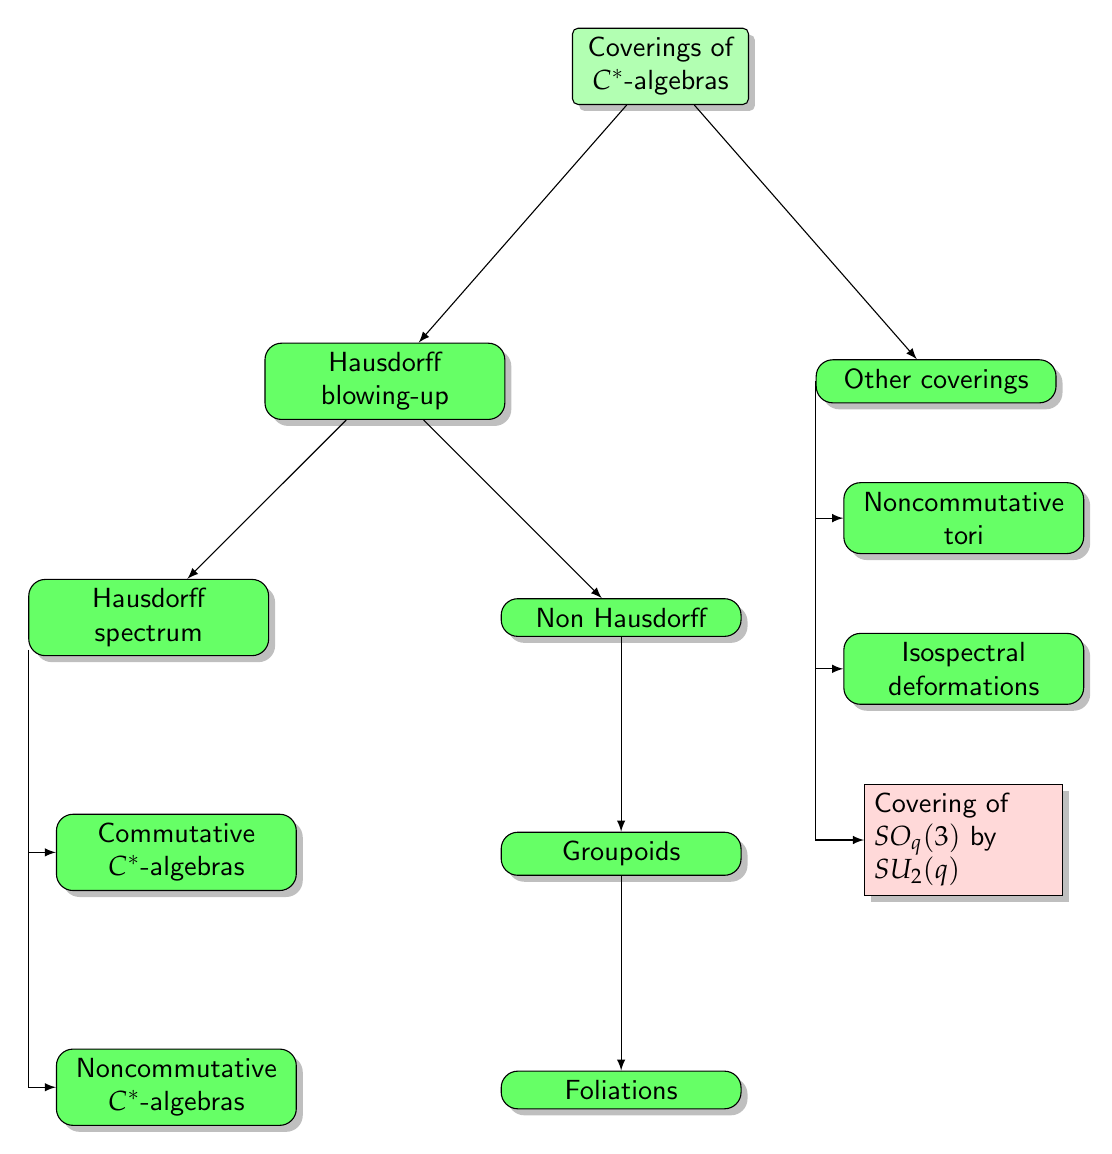
\begin{tikzpicture}[
		level 1/.style={level distance = 4.0cm,sibling distance=70mm, node distance=100mm},
		level 2/.append style={level distance = 3cm, sibling distance=60mm, node distance=20mm},		
		level 3/.append style={level distance = 3cm, sibling distance=50mm, node distance=20mm},
		edge from parent/.style={->,draw},
		>=latex]
		% root of the the initial tree, level 1
		\node[root] {Coverings of $C^*$-algebras}
		% The first level, as children of the initial tree
		child {node[level 2] (ch1) {Hausdorff blowing-up}
			child {node[level 2] (c1) {Hausdorff spectrum}}
			child {node[level 2] (c2) {Non Hausdorff}}{
				child {node[level 2] (c3) {Groupoids}}{
					child {node[level 2] (c4) {Foliations}}
				}
			}
		}
		child {node[level 2] (ch2) {Other coverings}
		};
		\begin{scope}%[every node/.style={level 2}]
			\node [below = of  ch2, style={level 2}, xshift=10pt] (ch21) {Noncommutative tori};
			\node [below = of  ch21, style={level 2}] (ch22) {Isospectral deformations};
			\node [below = of  ch22, style={level 3}]  (ch23) {Covering of $SO_q(3)$ by $SU_2(q)$};
		\end{scope}	
		\begin{scope}[every node/.style={level 2}]
			\node [below = of  c1, xshift=10pt] (c11) {Commutative $C^*$-algebras};
			\node [below = of  c11] (c12) {Noncommutative $C^*$-algebras};
		\end{scope}	
		\foreach \value in {1,...,2}
		\draw[->] (c1.195) |- (c1\value.west);	
		\foreach \value in {1,...,3}
		\draw[->] (ch2.180) |- (ch2\value.west);
	\end{tikzpicture}	
	\caption{Classification of known noncommutative coverings} \label{fig:M1}
\end{figure}


\paragraph{}There are theories of coverings of $C^*$-algebras which can be included into a following list (cf. Figure \ref{fig:M1}):
\begin{itemize}
	\item coverings of commutative $C^*$-algebras  \cite{clarisson:phd,pavlov_troisky:cov},
	\item coverings of $C^*$-algebras of groupoids and foliations  \cite{ouchi:cov_fol,xiaolu:foli_cov,zhi:cov_group}),
	\item  coverings of noncommutative tori \cite{clarisson:phd,schwieger:nt_cov},
	\item {the double covering of the quantum group $SO_q(3)$} \cite{dijkhuizen:so_doublecov,podles:so_su}. 
\end{itemize}

This work is devoted to a single general theory which includes all theories of this list, i.e. we develop a  system of axioms which can be applied for every item of the list.

A commutative Gelfand-Na\u{i}mark theorem \cite{arveson:c_alg_invt} states a duality correspondence between  locally compact Hausdorff topological spaces and commutative $C^*$-algebras. So  a noncommutative $C^*$-algebra can be regarded as a noncommutative generalization of a topological space. Further development of the noncommutative geometry gives generalizations of following classical geometric and topological notions.
\break
\begin {table}[H]
\caption {Mapping between classical and noncommutative geometry} \label{main_mapping_table} 
\begin{center}
\begin{tabular}{|c|c|}
	\hline
Classical notion & Noncommutative generalization\\
	\hline
	&\\
	Topological space & $C^*$-algebra\\
	&\\
	Measure space & von Neumann algebra\\
	&\\	Riemannian manifold  & Spectral triple\\
	&\\	Topological $K$-theory & $K$-theory of $C^*$-algebras \\
	&\\	Homology and cohomology & Noncommutative homology and cohomology\\
	&\\
	\hline
\end{tabular}
\end{center}
\end {table}
\pagebreak
In this book we continue development of the noncommutative geometry, this book contains generalizations of following notions.

\begin {table}[H]
\caption {Mapping between geometry of topological coverings and noncommutative ones} \label{add_mapping_table} 
\begin{center}
\begin{tabular}{|c|c|}
	\hline
	Classical notion & Noncommutative generalization\\
	\hline
	&\\
	Covering & Noncommutative covering\\
	&\\
	Theorem about covering & 	Theorem about covering \\
 of Riemannian manifold & of spectral triple\\
	&\\
	Fundamental group of a space $\pi_1\left(\mathcal X \right)$  & Fundamental group of a $C^*$-algebra $\pi_1\left(A \right)$  \\
	& \\
%$n^{\text{th}}$ {homotopy group} $\pi_n\left(\sX, x_0 \right)$&$n^{\text{th}}$ {homotopy group} $\pi_n\left(A, \a \right)$ 
%	\\ of a  pointed space $\left(\sX, x_0 \right)$ & of a  pointed  $C^*$-algebra $\left(A, \a \right)$\\
%	&\\
	Hurewicz homomorphism &  Noncommutative	Hurewicz 
	\\ $\pi_1\left(\sX, x_0 \right)\to K_1\left( \sX\right)  $ & homomorphism $\pi_1\left(A \right)\to K_1\left(A\right)  $\\
	&\\
	
Flat connections given by & Noncommutative flat connections\\
 coverings & given by noncommutative coverings\\
	&\\
Unoriented  Spin$^c$-manifolds  & Unoriented  spectral triples\\
&\\
	\hline
\end{tabular}
\end{center}
\end {table}

\paragraph*{}
In contrary of the explained in  \cite{clarisson:phd,schwieger:nt_cov} results the presented here theory gives results which are (almost) equivalent to the classical topological theory. In particular covering spaces of commutative spaces are also commutative. This fact yields pure algebraic definition of the fundamental group   (cf. Theorem \ref{comm_uni_lim_thm}).% and the $n^{\text{th}}$-homotopy group (cf. Theorem \ref{ho_gr_thm}).
\paragraph*{}
The Part \ref{math_part} is devoted to mathematical aspects of the theory.
\paragraph*{}
The Chapter \ref{prel_chap} contains preliminary results. The material of this chapter can be read as needed.
\paragraph*{}
The Chapter \ref{cov_fin_chap} contains the construction of noncommutative    finite-fold coverings of $C^*$-algebras and operator spaces. Sections \ref{cov_fin_bas_sec} - \ref{induced_repr_fin_sec} are basic and needed for the further reading of this book. Other sections are written for  those who are interested in following applications of this theory:
\begin{itemize}
	\item Coverings and strong Morita equivalence.
	\item  Noncommutative path lifting.
	\item Coverings of spectral triples.
	\item Finite noncommutative coverings and flat connections.
	\item Unoriented spectral triples.
\end{itemize}
\paragraph*{}
The Chapter \ref{infinite_covering_chap} is devoted to  noncommutative   infinite coverings of $C^*$-algebras and operator spaces. The Sections \ref{infinite_ca_sec} - \ref{inf_mor_sec} are  basic. The Section \ref{str_cov_glo_sec} is interesting for  those who are interested in coverings of spectral triples.
\paragraph*{}
The Chapter \ref{top_chap} contains applications of described in Chapters  \ref{cov_fin_chap} and \ref{infinite_covering_chap} theory to commutative $C^*$-algebras. It is constructed a given by the Table \ref{add_mapping_table}   natural one to one correspondence between geometry of topological coverings and "noncommutative" ones.


\paragraph*{} The Chapter \ref{h_chap} is devoted to the generalization of the Hurewicz homomorphism from the fundamental group to $K$-homology.
\paragraph*{}
The Chapter \ref{blowing_chap} is devoted  to the construction of  Hausdorff blowing-up. This construction can be applied for obtaining of noncommutative coverings of  $C^*$-algebras with Hausdorff spectrum, and non-Hausdorff one, e.g. $C^*$-algebras of groupoids and foliations (cf. \cite{candel:foliII}).

%\paragraph*{}
%In the Chapter \ref{hurewicz_gr_chap} we consider the quantization of homotopy groups explained in \cite{spanier:at,switzer:at}. It is proven that homotopy groups can be calculated by purely algebraic methods. 
\paragraph*{}
In the Chapter \ref{stab_chap} it is proven that some properties of noncommutative coverings are stably invariant. 
%\paragraph*{}
%In the Chapter \ref{stab_chap} we prove that if $*$-homomorphism $A \hookto \widetilde{A}$ of $C^*$-algebras is a "noncommutative covering" then both natural $*$-homomorphisms  $A \otimes \mathbb{M}_n\left(\C \right)  \hookto \widetilde{A} \otimes \mathbb{M}_n\left(\C \right)$ and $A \otimes \K\left(\ell^2\left( \N \right)\right)  \hookto \widetilde{A}\otimes \K\left(\ell^2\left( \N \right)\right)$ are "noncommutative coverings".

\paragraph*{} The Chapter \ref{ctr_chap} is devoted to noncommutative coverings of $C^*$-algebras with Hausdorff spectrum. It is proven that the theory of noncommutative coverings of $C^*$-algebras with Hausdorff spectrum contains all ingredients of right row of the Table \ref{add_mapping_table}. 



%\paragraph*{} In the  Chapter \ref{vf_chap} the coverings of spaces of vector fields are being discussed. Sections of vector fields of Hilbert spaces have the natural structure of operator spaces. Application of the results of the Chapters \ref{cov_fin_chap}  and \ref{infinite_covering_chap} yield finite-fold and infinite noncommutative coverings of these spaces.

\paragraph*{} In the Chapter \ref{foliations_chap} we consider noncommutative finite-fold and infinite coverings of $ C^*$-algebras of groupoids and foliations. 

\paragraph*{} The Chapter \ref{nt_chap} is devoted to noncommutative coverings of noncommutative tori.% In particular we find a stable fundamental group and Hurewicz homomorphism of noncommutative tori.


\paragraph*{} The Chapter \ref{isospectral_chap} is devoted to noncommutative coverings of isospectral deformations. We consider "noncommutative finite-fold coverings" only. The presented in Sections \ref{triple_fin_cov}, \ref{flat_sec} and \ref{unoti_defn_sec} theory of coverings of spectral triples is applied to isospectral deformations.
\paragraph*{} 
The Chapter \ref{qdr_chap} is devoted to  noncommutative coverings of quantum groups.

\paragraph*{} In the Part \ref{phys_part} we consider related to the theoretical physics math models.


\paragraph*{}
In the Chapter \ref{haus_non_haus_dul_sec} we show Hausdorff - non Hausdorff duality, i.e. a $C^*$-algebra with non Hausdorff spectrum can have a covering  $C^*$-algebra with  Hausdorff spectrum. In principle having physical models with 
Hausdorff spectrum one can  construct physical models with 
non Hausdorff spectrum.
\\paragraph*{}
The Chapter \ref{wl_chap} is devoted to Wilson lines over  noncommutative spaces.

\tableofcontents

\part{Mathematical theory}\label{math_part}
\chapter{General Theory}
\section{The Gelfand space of $C^*$-algebra}

	
	If $A$ is $C^*$-algebra then from the Lemma \ref{hered_ideal_lem} it follows that the a meet-semilattices (cf. Definition \ref{lattice_defn}) or closed left, right ideals and hereditary $C^*$-subalgebras are isomorphic.
	If  $\mathfrak{Gelfand}\left(A \right)$  is a set of ultrafilters of these the meet-semilattices then denote by
	\be\label{gelfand_eqn}
	\begin{split}
		\mathfrak{Gelfand}\left(A \right)_{I} \bydef \left\{\left. x \in \mathfrak{Gelfand}\left(A \right)\right| I \in x\right\},\\
		\mathfrak{Gelfand}\left(A \right)_{B} \bydef \left\{\left. x \in \mathfrak{Gelfand}\left(A \right)\right| B \in x\right\}
	\end{split}
	\ee
where $I$ is a one-sided ideal, $B$ is a hereditary $C^*$-algebra.	



\begin{lemma}
There is the natural topology on  $\mathfrak{Gelfand}\left(A \right)$ generated by the sets \eqref{gelfand_eqn} (cf. Definition \ref{top_base_defn})
\end{lemma}
\begin{proof}
	One needs check conditions (a) and (b) of the Definition \ref{top_base_defn}.\\
	(a) Evident.\\
	(b)  If $x \in \mathfrak{Gelfand}\left(A \right)_{B_1}\cap \mathfrak{Gelfand}\left(A \right)_{B_2}$ then $B_1\in x$ and $B_{2} \in x$ then from the Definition \ref{filter_defn} it %turns out that 	$x \in \mathfrak{Gelfand}\left(A \right)_{B_{1}}\cap B_{{2}}$.
\end{proof}

	\begin{definition}\label{gelfand_space_defn}
Under the above hypothesis $\mathfrak{Gelfand}\left(A \right)$ is the \textit{Gelfand space} of $A$.
\end{definition}
\begin{remark}\label{gelfand_space_rem}
According to the \ref{hered_ideal_lem}	the Definition \ref{gelfand_space_defn} can use closed left (right) ideals instead of hereditary subalgebras. For any closed left ideal $I$ the following notation will be used
\be\label{gelfand_ideal_eqn}
\begin{split}
x \in I,\\
\mathfrak{Gelfand}\left(A \right)_I \bydef \left\{\left. x \in \mathfrak{Gelfand}\left(A \right)\right| I \in x\right\}
\end{split}
\ee
\end{remark}
\begin{thm}\label{gelfand-naimark_thm}\cite{arveson:c_alg_invt} (Commutative Gelfand-Na\u{\i}mark theorem). 
	Let $A$ be a commutative $C^*$-algebra and let $\mathcal{X}$ be the spectrum of A. There is the natural $*$-isomorphism $\gamma:A \xrightarrow{\cong} C_0(\mathcal{X})$.
\end{thm}


\begin{lemma} (Generalized commutative Gelfand theorem).
If $\sX$ is a compact Hausdorff space then  is a natural  homeomorphism $\mathfrak{Gelfand}\left(C\left( \sX\right)  \right)\cong \sX$.
	\end{lemma}
	\begin{proof}
		From the Lemma \ref{hered_ideal_lem} there is a one-to-one correspondence between hereditary $C^*$-subalgebras and closed left ideals. However every closed left ideal is a closed two-sided ideal and vice versa. The  meet-semilattice of  hereditary $C^*$-subalgebras is naturally isomorphic to  the  meet-semilattice of closed two sided ideals. From the theorem \ref{gelfand-naimark_thm} it follows that these both semi-lattices are naturally isomorphic to the semilattice of open sets of $\sX$. Now this lemma is a consequence of the Lemma \ref{top_ultra_thm}.
	\end{proof}

\begin{definition}\label{hereditary_extension_defn}
	If both be $A$ and $\widetilde{A}$ be $C^*$-algebras then  a *-homomorphism
	\bean
	\varphi: A \hookto M\left(\widetilde A\right)
	\eean
	is said to be a \textit{hereditary full} if a set $\varphi\left( A\right) \widetilde{A} \varphi\left(A \right)$ is dense in  $\widetilde A$. Equivalently a left ideal $\widetilde{A} \varphi\left(A \right)$  of $\widetilde{A}$ is dense in $\widetilde{A}$.
\end{definition}



\begin{lemma}\label{lolale_lem}
	Any hereditary injective  *-homomorphism 	
	\bean
	\varphi: A \hookto M\left(\widetilde A\right)
	\eean
	naturally yields a continuous mapping 
	\bean
	\mathfrak{Gelfand}\left(\widetilde A \right)\xrightarrow{\mathfrak{Gelfand}\left(\varphi \right)}\mathfrak{Gelfand}\left(A \right)
	\eean
\end{lemma}
\begin{proof}
If both  $\mathfrak{Lattice}\left(A \right) $ and $\mathfrak{Lattice}\left(\widetilde A \right)$ are meet-semilattices of closed left ideals of $A$ and $\widetilde A$ then the mapping
\bean
\mathfrak{Lattice}\left(A \right)\xrightarrow{\mathfrak{Lattice}\left(\varphi \right)} \mathfrak{Lattice}\left(\widetilde A \right),\\
\widetilde I \mapsto \\
\bigcap \left\{I \subset A~  \text{is left ideal} \left| \widetilde I \subset C^*\text{-norm completion of } \widetilde A \varphi\left( I\right)\right.\right\}
\eean 
is a homomorphism of meet-semilattices such that 
\be
I_1 \cap  I_2 \neq \{0\}\quad \Rightarrow\quad \mathfrak{Lattice}\left(\varphi \right) \left(I_1 \cap I_2  \right)\neq \{0\} 
\ee
If both  $\mathfrak{Filter}\left(A \right) $ and $\mathfrak{Filter}\left(\widetilde A \right)$ are sets of filters of $\mathfrak{Lattice}\left(A \right) $ and $\mathfrak{Lattice}\left(\widetilde A \right)$ then there is a mapping
\bean
\mathfrak{Filter}\left(\widetilde A \right)\xrightarrow{\mathfrak{Filter}\left(\varphi\right)} \mathfrak{Filter}\left( A \right),\\
\Psi \mapsto \text{ the filer generated by } \mathfrak{Lattice}\left(\varphi \right)^{-1}\left(\Psi \right).
\eean
From the Lemma \ref{hered_ideal_lem} it !!!! 
 For any  $x \in  \mathfrak{Gelfand}\left( A \right)$ consider a set
\bean
\mathfrak{Gelfand}\left( A \right)_x \bydef
\left\{\left. \widetilde x \in \mathfrak{Gelfand}\left(\widetilde A \right)\right| \exists \widetilde \Psi \in \mathfrak{Filter}^{-1}\left( x\right)\quad  \widetilde \Psi \subset x  \right\}
\eean
The map $\mathfrak{Gelfand}\left(\varphi \right)$ we define by the following way
$$
\forall \widetilde  x \in \mathfrak{Gelfand}\left( A \right)_x\quad  \mathfrak{Gelfand}\left( \varphi \right)\left( \widetilde  x\right) = x.
$$
Any left closed ideal $I$ with $I \in x$ yields an ideal $\widetilde I\bydef\mathfrak{Lattice}\left(\varphi \right)\left(I \right)$ such that
$$
\mathfrak{Gelfand}\left( \varphi \right)^{-1}\left(\left\{\left. x \in \mathfrak{Gelfand}\left( A\right)\right| I \in x \right\} \right) =\left\{\left. \widetilde y \in \mathfrak{Gelfand}\left( \widetilde A\right)\right| \widetilde I \in \widetilde y \right\}
$$ 
From the above equation it turns out that the mapping $\mathfrak{Gelfand}\left( \varphi \right)$ is continuous.
\end{proof}

\begin{empt}
For any $x \in 	\mathfrak{Gelfand}\left( \widetilde A\right)$ consider a set of left ideals 
$$
X_x \bydef \left\{ I \subset A \left| I \text{ is left a ideal AND } \exists I' \in x \quad I'\cap I =\{0\} \right.\right\}
$$
\end{empt}
\begin{definition}\label{orthogonal_defn}
	The $C^*$-norm closure $I^\perp_x$ of the generated by the set $X_x$ left ideal  is the \textit{orthogonal to} $x$ \textit{ideal}.
The hereditary $C^*$subalgebra $A^\perp_x \bydef I^\perp_x\cap \left( I^\perp_x\right)^*$	is  the \textit{orthogonal to} $x$ \textit{subalgebra}.
\end{definition}
\begin{remark}\label{orthogonal_rem}
	For any maximal left ideal $I\subset A$ there is $x \in \mathfrak{Gelfand}\left( A \right)$ such that
	$$
x = \left\{I' \subset A\left|  I' \text{ is left a ideal AND } I'\cap I \neq I'\right.\right\}	
	$$
	The space 	$\mathfrak{Gelfand}\left( \widetilde A\right)$ can be regarded as a set of maximal left ideals and the basis of topology contains sets
	$$
X_I \left\{I'\left| I' \text{ is a maximal ideal } I \subset I \right.\right\}
	$$
	where $I$ is closed left Ideal.
	
	
\end{remark}
\be\label{lideal_eqn}
\begin{split}
	I\subset Aa,\\
	B \subset aAa
\end{split}	
\ee	
where $a \in \K\left( A\right)_+$ is a positive element of Pedersen's ideal.
Both these sets are  
where $I$ and $B$ satisfy to the equations \eqref{lideal_eqn}.
\section{Coverings and fundamental group}
\subsection{Topologies of *-automorphisms groups}

where $\mathrm{Homeo}$ means the group of homeomorphisms with {compact-open} topology (cf \ref{top_comp_open_empt}). Above diagram has the following noncommutative generalization   
\newline
\hspace*{\fill}
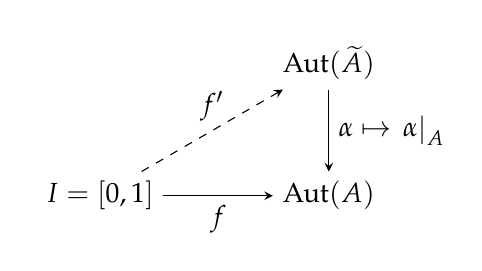
\begin{tikzpicture}
	\matrix (m) [matrix of math nodes,row sep=3em,column sep=4em,minimum width=2em] {
		& \Aut(\widetilde{A}) \\
		I = [0,1]  & \Aut(A) \\};
	\path[-stealth]
	(m-2-1.east|-m-2-2) edge node [below] {$f$}(m-2-2)
	(m-1-2) edge node [right] {$\al \mapsto \left.\a\right|_{A}$} (m-2-2)
	(m-2-1)      edge [dashed]  node[above] {$f'$} (m-1-2);
\end{tikzpicture}
\hspace{\fill}
\newline
In the above diagram we require that $\al|_A \in \mathrm{Aut}\left(A\right)$ for any $\al \in \mathrm{Aut}\left(\widetilde{A}\right)$. The diagram means that $f'(t)|_{A} = f(t)$ for any $t \in [0,1]$. Noncommutative generalization of a locally compact space is a $C^*$-algebra, so  the generalization of $\mathrm{Homeo}(\mathcal{X})$ is the group  $\mathrm{Aut}(A)$ of $*$-automorphisms carries (at least) two different topologies making it into a topological group \cite{thomsem:ho_type_uhf}. The most important is {\it the topology of pointwise norm-convergence} based on the open sets
\begin{equation*}
	\left\{\left.\alpha \in \mathrm{Aut}(A) \ \right| \ \|\alpha(a)-a\| < 1 \right\}, \quad a \in A.
\end{equation*}
The other topology is the {\it uniform norm-topology} based on the open sets
\begin{equation}\label{aut_norm_eqn}
	\left\{\alpha \in \mathrm{Aut}(A) \ \left| \ \sup_{a \neq 0}\ \|a\|^{-1} \|\alpha(a)-a\| < \varepsilon \right. \right\}, \quad \varepsilon > 0
\end{equation}
which corresponds to following "norm"
\begin{equation}\label{uniform_norm_topology_formula_eqn}
	\|\alpha\|_{\text{Aut}} = \sup_{a \neq 0}\ \|a\|^{-1} \|\alpha(a)-a\| = \sup_{\|a\| =1}\  \|\alpha(a)-a\|.
\end{equation}
Above formula does not really means a norm because $\mathrm{Aut}\left(A\right)$ is not a vector space. Henceforth the uniform norm-topology will be considered only.
\subsection{Basic definitions}
  \begin{definition}\label{connected_c_a_defn}
	We say that a $C^*$-algebra $A$ is \textit{connected} if it cannot be represented as a direct sum  $A \cong A' \oplus A''$ of nontrivial $C^*$-algebras $A'$ and $A''$.
	
	% (the Gelfand spectrum of the center of $M\left( A\right) $ is connected). Let $A \subset B$ be a connected subalgebra. We say that $A$ is a \textit{connected component} of $B$ if  $1_{M\left( A\right) }$ lies in the center of $1_{M\left( B\right) }$.
\end{definition}

  \begin{definition}\label{fin_quasi_defn}
	Let both  $A$ and  $\widetilde{A}$ be  connected $C^*$-algebras (cf. Definition \ref{connected_c_a_defn}), and let $\lift: A \hookto \widetilde{A}$ be an injective $*$-homomorphism of % connected	  
	$C^*$-algebras. Let $G$ be a finite  group of $*$-automorphisms of $\widetilde{A}$ such that 	$\lift\left(A\right) = \widetilde{A}^G\stackrel{\text{def}}{=}\left\{
	\left.a\in \widetilde{A}~\right|~ a = g a;~ \forall g \in G\right\}$.	We say that the triple $\left(A, \widetilde{A}, G \right)$ and/or the quadruple $\left(A, \widetilde{A}, G, \lift \right)$ and/or $*$-homomorphism $\lift: A \hookto \widetilde{A}$   is a \textit{noncommutative  quasi-covering}. We write
	\be\label{fin_cov_gr_eqn}
	G\left(\left.\widetilde{A}~\right| {A} \right) \stackrel{\text{def}}{=}  	G.
	\ee
\end{definition}

   \begin{definition}\label{fin_pre_defn}
	Let   $A$ be an unital connected $C^*$-algebra  and let  $\widetilde{A}$ be  connected $C^*$-algebra (cf. Definition \ref{connected_c_a_defn}), and let $\lift: A \hookto M\left( \widetilde{A}\right) $ be an injective  $*$-homomorphism of % connected
	$C^*$-algebras such that following conditions hold:
	\begin{enumerate}
		\item[(a)] if $\Aut\left(\widetilde{A} \right)$ is a group of $*$-automorphisms of $\widetilde{A}$ then the group  
		\be\nonumber
		G \bydef \left\{ \left.g \in \Aut\left(\widetilde{A} \right)~\right|\forall a \in \lift \left( A\right) \quad ga = a\right\}
		\ee
		is discrete
		\item[(b)] 	$A = \widetilde{A}^G\stackrel{\text{def}}{=}\left\{\left.a\in \widetilde{A}~~\right|\forall g \in G\quad  a = g a\right\}$.
	\end{enumerate}
	We say that the triple $\left(A, \widetilde{A}, G \right)$ and/or the quadruple $\left(A, \widetilde{A}, G, \lift \right)$ and/or $*$-homomorphism $\lift: A \hookto \widetilde{A}$   is a \textit{noncommutative  pre-covering}. We write $G\left(\left.\widetilde A~\right|A \right)\bydef G$.
\end{definition}

\begin{definition}\label{evenly_defn}
	
Let $\left(A, \widetilde{A}, G, \lift \right)$ be a noncommutative  pre-covering (cf. Definition \ref{fin_pre_defn})
	A connected hereditary $C^*$-subalgebra $B \subset A$ 
	is $\left(A, \widetilde{A}, G, \lift \right)$- \textit{evenly covered by} $\left(A, \widetilde{A}, G, \lift \right)$ if there is a hereditary $C^*$-subalgebra $\widetilde B \subset \widetilde A$ with a $*$-isomorphism $\lift^{\widetilde B}: B \cong \widetilde B$ such that
	\be\label{evenly_eqn}
	\forall b \in B \quad \lift\left( b\right) = \bt \text{-}\sum_{g\in G} g \lift^{\widetilde B}\left( b\right) 
	\ee
where $\bt \text{-}\sum$ means the convergence with respect to the strict topology of $M\left( \widetilde A\right)$ (cf. Definition \ref{strict_topology_defn}) 	
\end{definition}

\begin{definition}\label{cov_unital_defn}
	
A  noncommutative  pre-covering $\left(A, \widetilde{A}, G, \lift \right)$ (cf. Definition \ref{fin_pre_defn}) with unital $A$ is a {\it unital noncommutative covering} if for any $x \in \mathfrak{Gelfand}\left(A \right)$ there is a hereditary connected $C^*$-subalgebra of $B$ {evenly covered by} $\left(A, \widetilde{A}, G, \lift \right)$ with $B \in x$
\end{definition}

\begin{definition}\label{cov__defn}
	
	A  noncommutative finite-fold pre-covering $\left(A, \widetilde{A}, G, \lift \right)$ (cf. Definition \ref{fin_pre_defn})  {\it noncommutative  covering} if there is 
	if there is an unital noncommutative covering $\left(B, \widetilde{B}, G, \widetilde\lift \right)$  with inclusions $A \subset B$ and $\widetilde A \subset \widetilde B$ such that:
\begin{enumerate}
	\item [(a)] both $A$ and $B$ are essential ideals of $B$ and $\widetilde B$,
	\item[(b)] $\lift \bydef \left.\widetilde\lift\right|_A$,
	\item[(c)] the action $G \times \widetilde B \to \widetilde B$ naturally comes from the $G \times \widetilde A \to \widetilde A$
\end{enumerate}	
\end{definition}





\chapter{Applications}
\section{Hausdorff blowing-up}
\begin{definition}\label{blowing_up_defn}
	For any $C^*$-algebra $A$ 
	an inclusion $C_0\left( \sX\right) \hookto M\left(A \right)$ into multiplier $C^*$-algebra  such that
	$$
	C_0\left( \sX\right)AC_0\left( \sX\right)
	$$
	is dense in $A$.
\end{definition}
The "blowing-up" word is inspired by following reasons.
\begin{itemize}
	\item Sometimes there is  the natural partially defined  surjective  map from  Hausdorff blowing-up to the spectrum.
	\item  In the algebraic geometry   "blowing-up" means  excluding of singular points  (cf. \cite{hartshorne:ag}).
\end{itemize}
\begin{remark}\label{c_i0_rem}
	If $C_0\left( \sX\right) \hookto M\left(A \right)$ is  \textit{Hausdorff blowing-up of } $A$ then form the Lemma \ref{lolale_lem} it follows that there is a geometric morphism $\mathfrak{Topos}\left( A\right)\xrightarrow{f}\mathfrak{Topos}\left(C_0(\sX)\right)$.  If $F$ is an Abelian group then from the  Proposition \ref{spectral_sequence_prop} for any $r\ge 0$ there is a homomorphism
	\bean
	H^r\left(\mathfrak{Topos}\left( C_0\left( \sX\right)\right) , F \right) \xrightarrow{} H^r \left(\mathfrak{Topos}\left( A\right), f^*\mathfrak{Ass} \left( F_A\right)\right).
	\eean
	From the Remark \ref{c_0_x_rem} it follows that $\mathfrak{Space}\left(C_0\left( \sX\right)  \right) = \sX$, and tahing into account \eqref{hom_eqn} one has a homomorphism
	\be\label{hom_to_x_eqn}
	H^r\left(\sX, F \right) \xrightarrow{} H^r \left(A, f^*\mathfrak{Ass} \left( F_A\right)\right).
	\ee
	
\end{remark}

\begin{notation}
	If $C_0\left( \sX\right) \hookto M\left(A \right)$ is {Hausdorff blowing-up of } $A$ and $\sU \subset \sX$ is open subset then denote by
	\be
	_\sU A _\sU \bydef \text{ the generated by } C_0\left(\sU \right) A  C_0\left(\sU \right) \text{ hereditary subalgebra of } A.
	\ee
\end{notation}
For any $B \in \mathbf{Hered}/A$ denote by
\be\label{b_res_eqn}
B|_\sU \bydef B \cap~ _\sU A_\sU.
\ee

\begin{exercise}
	Let $\left\{\sU\right\}_{\iota \in I}$ be a family of open subsets of $\sX$ 	and let $\sU \bydef \cup_{\iota \in I}\sU_\iota$.
	Prove following statements:
	\begin{enumerate}
		\item a set   $\left\{_{\sU_\iota}A_{\sU_\iota}\right\}_{\iota \in I}$ is a covering of $_\sU A_\sU$ (cf. Definition \ref{hered_cov_defn}),
		\item  for any $B \in \mathbf{Hered}/A$ a set $\left\{B|_{\sU_\iota}\right\}_{\iota \in I}$ is a covering of $B|_\sU$ (cf. Equation \eqref{b_res_eqn}).
	\end{enumerate}
\end{exercise}





\section{$C^*$-algebras of type $I_0$}
\subsection{Gelfand spaces}
\paragraph{}
Here we prove that for   $C^*$-algebra of type $I_0$ (cf. Definition \ref{type_I_defn}) the  Grothendieck $A$-locale is spatial. 
\begin{remark}\label{comm_hered_gen_rem}
	From the Definition \ref{type_I_defn} it follows that any  $C^*$-algebra of type $I_0$ is generated by its commutative hereditary subalgebras.
\end{remark}
\begin{empt}
Let	$A$ be a $C^*$-algebra of type $I_0$ and let $x \in \mathfrak{Gelfand}\left(A \right)$. The set of hereditary subalgebras $B' \subset A$ with $B \notin x$ has a maximal element $B \subsetneqq A$. Since $A$ be a $C^*$-algebra of type $I_0$ there is a commutative subalgebra $C\left(\sY \right)$ with the natural inclusion $j:C\left( \sY\right) \hookto M\left( A\right)$ with
$$
j\left( C\left( \sY\right)\right) \neq j\left( C\left( \sY\right)\right)\neq 
$$
\end{empt}
\begin{definition}
	
	Let $A$ be a $C^*$-algebra of type $I_0$. An $A$-\textit{representative}  is a triple $\left( j, y, C_0\left( \sY\right) \right)$ where 
	\begin{enumerate}
		\item[(a)]  $j: C_0\left(\sY \right) \hookto A$ is an inclusion of $C^*$-algebras.
		\item[(b)] $y \in \sY$ is a point.
	\end{enumerate}
	For any open subset $\sU\subset \sY$ there is an inclusion $C_0\left(\sU\right)\subset C_0\left(\sY\right)$.
	Two $A$-{representatives} $\left( j', y',  C_0\left( \sY'\right)\right)$ and  $\left( j'', y'',  C_0\left( \sY''\right)\right)$ are \textit{equivalent} if there are open neighborhoods $\sU'$ and $\sU''$ of $x'$ and $x''$ respectively such that
	$$
	j'\left(C_0\left( 
	\sU'\right) \right) = j''\left(C_0\left( 
	\sU''\right) \right).
	$$
	Equivalence classes of representatives a said to be  $A$-\textit{points}. An $A$ point represented by  $\left( j,y,  C_0\left( \sY\right)\right)$   will be denoted by $\left[\left( j, y,  C_0\left( \sY\right)\right)\right]$.  We denote by $\mathfrak{Points}\left(A \right)$ a set of $A$-points.  
\end{definition}
\begin{lemma}\label{pgelfand_eqn}
	For any 	$\left[\left( j, y,  C_0\left( \sY\right)\right)\right]\in \mathfrak{Points}\left(B \right)$ the set of hereditary subalgebras
	\be
x \bydef \left\{B \subset A \left|\exists \mathrm{~open~neighborhood~} \sU \mathrm{~of~} y~ B \cap j\left( C_0\left( \sU\right)\right) = j\left( C_0\left( \sU\right)\right) \right.\right\}	
\ee
	is an ultrafilter.
\end{lemma}
\begin{proof}
	If $B_1\in x$ and $B_1 \subset B_2$ then from \eqref{pgelfand_eqn} it turns out that 
	If $B \notin x$ then there is an 
	if $f \in C_0\left( \sU\right)$ with $f\left(y \right) = 1$ and  $B \cap j\left( C_0\left( \sU\right)\right) = \{0\}$
	
	
	 then there is a ~open~neighborhood~ $\sU$ {~of~} $y$ with  $ B \cap j\left( C_0\left( \sU\right)\right) = \{0\}$. Otherwise $j\left( C_0\left( \sU\right)\right)\in x$ it follows that $B\notin x$. So $x$ is an ultrafilter.
\end{proof}	



\begin{theorem}\label{type_0_thm}
	If $A$ is a $C^*$-algebra of type $I_0$ then the Grothendieck $A$-locale $\mathfrak{Locale}(A)$ is spatial, and the Grothendieck $A$-space  $\mathfrak{Space}(A)$ is homeomorphic to $\mathfrak{Points}(A)$.
\end{theorem}
\begin{proof}
	From the Remark \ref{comm_hered_gen_rem} and the Lemma \ref{type_I_lem} it follows that the locale $\mathfrak{Locale}(A)$ is naturally isomorphic to a locale of open sets of the sober space $\mathfrak{Points}(A)$.
\end{proof}
\begin{exercise} Prove following statements.
	\begin{enumerate}
		\item For any $C^*$-algebra $A$ of type $I_0$ there is an isomorphism of locales
		$$
		\mathfrak{BohrLocale}(A)\cong \mathfrak{Locale}(A)	
		$$
		where $\mathfrak{BohrLocale}(A)$ is a Bohr $A$-locale (cf. Definition \ref{bohr_locale_defn}).
		\item From the Theorem 	\ref{comp_thm} it follows that there is $C^*$-algebra $A$ of type $I$ such that $\mathfrak{BohrLocale}(A)\subsetneqq\mathfrak{Locale}(A)$.
	\end{enumerate}
\end{exercise}
\begin{remark}
	From the inclusion $\mathfrak{BohrLocale}(A)\subsetneqq\mathfrak{Locale}(A)$ it follows that the Grothendieck $A$-locale can be more informative than the Bohr one.
\end{remark}
\begin{definition}\label{hered_cov_defn}
	For any $\mathbf{Hered}/A$-object $B$ a distinguished set of families of inclusions $\left\{B_\iota \subset B\right\}_{\iota\in I}$, called a \textit{covering} of $B$ if $B$ is a generated by the union $\cup B_\iota$ hereditary $C^*$-subalgebra of $A$ (cf. Definition \ref{hered_generated_defn}).
\end{definition}
\begin{rem}\label{cov_rem}
	If $A$ is a $C^*$-algebra of type $I_0$ and
	\be\label{ca_eqn}
	\mathscr C^A \bydef \left\{C \subset A | C \text{ is a hereditary commutative } C^*\text{-subalgebra of }  A\right\}.
	\ee
	then from the Remark \ref{comm_hered_gen_rem} it follows that the family $\mathscr C^A$ is a covering of $A$ (cf. Definition \ref{hered_cov_defn}).
\end{rem}
\subsection{Etal\'e Hausdorff blowing-up}
\paragraph*{}
If $A$ is a $C^*$-algebra of type $I_0$ and $C_0\left(\sX \right) \to M\left(A \right)$ is Hausdorff blowing-up then from the Lemma \ref{lolale_lem} it follows that there is a continuous map:
$p_A :\mathfrak{Space}(A)\to \sX$
(cf. Remark \ref{lolale_lem})
\begin{definition}\label{etale_haus_defn}
	If $A$ is a $C^*$-algebra of type $I_0$ then Hausdorff blowing-up $C_0\left(\sX \right) \to M\left(A \right)$ is said to be \textit{etal\'e} if the map
	\be\label{p_a_eqn}
	p_A: \mathfrak{Gelfand}(A)\to \sX
	\ee is a local homeomorphism.
\end{definition}

\begin{empt}
	We define a presheaf of sets $\mathscr{P}^A $ on $\sX$ (cf. Definition \ref{presheaf_defn}) such that for any pair  $\sV\subset\sU$ of open subsets of $\sX$ one has
	\be\label{comm_alg_sheaf}
	\begin{split}
		\mathscr{P}^A\left( \sU\right) \bydef \left\{C\cap~ _\sU A_\sU\left| C \in \mathscr C^A \right. \right\}= \left\{\left.C\in \mathscr C^A \right| C \subset~ _\sU A _\sU \right\};\\
		\rho_{\sU \sV}: \mathscr{P}^A \left(\sU\right)\to  \mathscr{P}^A \left(\sV\right), \quad C \mapsto C \cap~_\sV A_{\sV}.
	\end{split}
	\ee
	\begin{remark}\label{flabby_rem}
		We denote by
		\be\label{c_res_eqn}
		C|_\sU \bydef C \cap~ _\sU A_\sU.
		\ee $\mathscr{P}^A$
		Since $C|_\sU$ is a hereditary $C^*$-subalgebra of $A$ the presheaf  $\mathscr{P}^A$  is flabby (cf. Definition \ref{sheaf_flabby_defn}),  so $\mathscr{P}^A$ is a sheaf (cf. Definition \ref{sheaf_defn}).
	\end{remark}
	
	Suppose that $A$ is a $C^*$-algebra of type $I_0$.
	Let $\mathrm{Sp\acute{e}}\left(\mathscr P^A  \right)$ be an	\'espace etal\'e  (cf. Exercise \ref{sheaf_etale_exer}) of the presheaf $\mathscr{P}^A$. 
	As a set the space  $\mathrm{Sp\acute{e}}\left(\mathscr P^A  \right)$ is a union of all stalks of the sheaf $\mathscr{P}^A$. There is a surjective local homeomorphism $p':\mathrm{Sp\acute{e}}\left(\mathscr P^A  \right)\to \sX$ (cf. Exercise \ref{sheaf_etale_exer}).
	For any commutative hereditary  $C^*$-subalgebra $C \in \mathscr C^A$ consider a union of open sets 
	\bean
	\mathscr U'_C \bydef \left\{ \left. y \in \mathrm{Sp\acute{e}}\left(\mathscr P^A \right) \right| y \quad \text{ is represented by}\quad  C\right\}.
	\eean
	(cf. n$^{\text{o}}$ 1 of the Exercise \ref{sheaf_etale_open_exer}) which is an open subset  $\mathrm{Sp\acute{e}}\left(\mathscr P^A\right)$.
	If $C^0\bydef \{0\}\subset A$ is the  trivial hereditary $C^*$-subalgebra, then the set $\mathscr U'_{C^0}$ is open. 
	
	\begin{theorem}
		Let $A$ is a $C^*$-algebra of type $I_0$ and $C_0\left(\sX \right) \to M\left(A \right)$ is etal\'e Hausdorff blowing-up (cf. Definitions \ref{blowing_up_defn} and \ref{etale_haus_defn}). If
		\be\label{xa_eqn}
		\mathscr X^A \bydef \mathrm{Sp\acute{e}}\left(\mathscr P^A \right)\setminus \mathscr U'_{C^0}
		\ee
		then there is the natural homeomorphism 
		$$
		\mathscr X^A \cong \mathfrak{Space}(A).
		$$
	\end{theorem}
	\begin{proof}
		From the Theorem \ref{type_0_thm} one has an isomorphism $\mathfrak{Space}(A)\cong \mathfrak{Points}(A)$. The map $p_{\mathscr X}:\mathfrak{Space}(A)\cong \mathfrak{Points}(A)\to \mathscr X^A$ is given by
		$$
		\left[\left( j, y,  C_0\left( \sY\right)\right)\right]\mapsto j\left( C_0\left( \sY\right)\right)_{p_A\left( \left[\left( j, y,  C_0\left( \sY\right)\right)\right]\right) }
		$$
		If not then there is an open neighborhood $\sU$ of $x \bydef p_A\left( \left[\left( j, y,  C_0\left( \sY\right)\right)\right]\right)$ such that
		$$
		C \bydef j\left(C_0\left( \sY\right) \right) \cap ~ _\sU A_\sU
		$$
		is a trivial $C^*$-algebra.
		Clearly $j\left( C_0\left( \sY\right)\right)_{p_A\left( \left[\left( j, y,  C_0\left( \sY\right)\right)\right]\right) }\in  \mathrm{Sp\acute{e}}\left(\mathscr P^A \right)$, one needs check that $$j\left( C_0\left( \sY\right)\right)_{p_A\left( \left[\left( j, y,  C_0\left( \sY\right)\right)\right]\right) }\in  \mathscr X^A.$$
		
		!!!!
		
		
		$C \bydef j\left(C_0\left( \sY\right) \right)\subset A$ is a commutative hereditary $C^*$-subalgebra. A set $\mathfrak{Points}(C)$ is an open neighborhood  of $\left[\left( j, y,  C_0\left( \sY\right)\right)\right]$. If $p_A: \mathfrak{Space}(A)= \mathfrak{Points}(A)\to \sX$ is given by \eqref{p_a_eqn} local homeomorphism and $\sU'$ is an open neighborhood of $p_A\left(\left[\left( j, y,  C_0\left( \sY\right)\right)\right] \right)$ then $p^{-1}\left(\sU' \right)$ is an open   neighborhood of $\left[\left( j, y,  C_0\left( \sY\right)\right)\right]$. The intersection $p^{-1}\left(\sU' \right)\cap \mathfrak{Points}(C)$ is also an open   neighborhood of $\left[\left( j, y,  C_0\left( \sY\right)\right)\right]$. The map $p_A$ is a local homeomorphism so there is an open neighborhood $\mathscr U$ of  $\left[\left( j, y,  C_0\left( \sY\right)\right)\right]$ such that
		\begin{itemize}
			\item $\mathscr U \subset p^{-1}\left(\sU' \right)\cap \mathfrak{Points}(C)$,
			\item $p_A$ homeomorphically maps $\mathscr U$ onto $\sU \bydef p_A\left(\mathscr U \right)$.
		\end{itemize}
	\end{proof}
	
	
	
	then a set
	\be\label{ctr_top_eqn}
	\mathscr U_C \bydef \mathscr U'_C \cap \mathscr X^A
	\ee
	is an open subset of $\mathscr X^A$. 
	Any hereditary commutative  subalgebra $C$ corresponds to a continuous  section
	$$
	s : \sX \to \mathrm{Sp\acute{e}}\left(\mathscr P^A \right)
	$$
	(cf. Exercise \ref{sheaf_etale_exer}). If $s\left(x \right)$ is known for every $x \in p'\circ \left(\mathscr X^A\right)$ such that  then  $s\left(x \right)= C^0_x$ for all $x \in p'\circ s\left( \mathscr U'_{C^0}\right)$, so one has the unique section $s : \sX \to \mathrm{Sp\acute{e}}\left(\mathscr P^A \right)$. Thus any commutative hereditary algebra can be uniquely defined by the given by \eqref{ctr_top_eqn} open set $\mathscr U_C$. If $B$ is a hereditary $C^*$-subalgebra of $A$ and
	$$
	\mathscr C^A_B \bydef \left\{C\cap B \left| C \in \mathscr C^A \right.\right\}.
	$$ 
	then from the Remark \ref{cov_rem} and the Lemma \ref{grothendieck_ca_lem} it follows that $B$ is generated by the union
	$
	\bigcup_{C \in \mathscr C^A_B} C
	$.
	The set 
	\be\label{ctr_top_e_eqn}
	\mathscr X^A_B \bydef \bigcup_{C \in 	\mathscr C^A_B } \mathscr U_{C }
	\ee
	is a union of open subsets $\mathscr U_{C}$, so it is open. If $\mathscr U\subset \mathscr X^A$ is an open set and
	$$
	\mathscr Y^A_{\mathscr U} \bydef  \left\{\left.C \in \mathscr C^A\right|  \mathscr U_C \subset \mathscr U\right\}
	$$
	then
	$
	\mathscr Y^A_{\mathscr X^A_B }=  \mathscr C^A_B.
	$
	For any open subset $\mathscr U \subset \mathscr X$ denote by $A_{\mathscr U}$ a hereditary $C^*$-subalgebra of $A$  generated by a union 
	$
	\bigcup_{C \in \mathscr Y^A_{\mathscr U}} C$. From our construction it follows that $A_{\mathscr X^A_B}$ is generated by the union 
	$$
	\bigcup_{C \in \mathscr Y^A_{\mathscr X^A_B}} C= \bigcup_{C \in \mathscr C^A_B} C.
	$$
	Since  $B$ is also generated by the union $ \bigcup_{C \in \mathscr C^A_B} C$  one has
	\be\label{one_to_one_eqn}
	A_{\mathscr X^A_B} = B.
	\ee
	Let $\Om_\sX$ be {sheaf of stalks of open sets} (cf. Appendix \ref{open_sheaf_empt}). Let  $\mathrm{Sp\acute{e}}\left(\Om_\sX \right)$ be the	\'espace etal\'e  (cf. Exercise \ref{sheaf_etale_exer}) of $\Om_\sX$ with the natural surjective local homeomorphism
	\be	\label{px_eqn}
	P_\sX :  \mathrm{Sp\acute{e}}\left(\Om_\sX \right)\to \sX
	\ee
	
	
	
\end{empt}

\begin{lemma}\label{section_lem}
	If  $A$ is a  $C^*$-algebra of the type $I_0$ with  {Hausdorff blowing-up} $C_0\left( \sX\right) \hookto M\left(A \right)$ then any commutative hereditary $C^*$-subalgebra is given by a section $s \in  \mathscr P^A\left( \supp C\right)$.
\end{lemma}
\begin{proof}
	From the equation \eqref{comm_alg_sheaf} it turns out that $C$ corresponds to a global section $s' : \sX \to \mathrm{Sp\acute{e}}\left(\mathscr P^A  \right)$. If $s^0 : \sX \to \mathrm{Sp\acute{e}}\left(\mathscr P^A  \right)$ is a section of the trivial subalgebra $C^0\bydef \{0\}\subset A$ then denote by 
	$$
	\sU_0 \bydef \left\{x \in \sX | s\left(x\right)= s_0\left( x\right) \right\}
	$$
	If $x \notin \sU_0$ then $\sV \cap \supp C \neq \emptyset$ for any open neighborhood $\sV$ of $x$.  So a union $\sU_0 \cup \supp C$ is dense in $\sX$. If the restriction $s \bydef s'|_{\supp C}$ is known then
	$$
	s'|_{\sU_0 \cup \supp C}= \begin{cases}
		s\left( x \right) & x \in \supp C\\
		s^0\left(x\right) & a \in \sU_0
	\end{cases}.
	$$
	Since the union $\sU_0 \cup \supp C$ is dense in $\sX$ the section $s'|_{\sU_0 \cup \supp C}$ uniquely defines $s'$. So the section $s$ uniquely defines both $s'$ and $C$.
\end{proof}


\begin{theorem}\label{grot_type_I_thm}
	If  $A$ is a  $C^*$-algebra of the type $I_0$ with  {Hausdorff blowing-up} $C_0\left( \sX\right) \hookto M\left(A \right)$ then one has:
	\begin{enumerate}
		\item [(i)] the space $\mathscr X^A$ is the Grothendieck $A$-space $\mathfrak{Space}\left(A \right)$ (cf. Definition \ref{grothendieck_ca_t_defn}),
		\item[(ii)] there is the natural surjective local homeomorphism
		\bea\label{pa_eqn}
		P_A: \mathscr X^A\to \mathrm{Sp\acute{e}}\left(\Om_\sX \right).
		\eea
	\end{enumerate}
\end{theorem}
\begin{proof}
	(i) From the equation  \eqref{one_to_one_eqn} it follows that there is a natural one to one correspondence 
	$$
	B \leftrightarrow A_{\mathscr X^A_B}
	$$
	between hereditary subalgebras of $A$ and open subsets of $\mathscr X^A$. So a category of open hereditary subalgebras of $B$ and their inclusions is equivalent to the category of open subsets of ${\mathscr X^A}$ and their inclusions.
	
	If  $\left\{\mathscr U_\iota\right\}_{\iota \in I}$ is a family of open sets of $\mathscr X^A$ such that $\mathscr U = \cup \mathscr U_\iota$ then for all $\iota \in I$ one has  $A_{\mathscr U_\iota}\subset  A_{\mathscr U}$. It turns out that
	\bean
	\forall\iota\in I \quad  L\left( A_{\mathscr U_\iota}\right) \subset L\left(A_{\mathscr U}\right),
	\eean
	\be\label{e_uu_eqn}
	\sum_{\iota\in I}L\left( A_{\mathscr U_\iota}\right) \subset L\left(A_{\mathscr U}\right)
	\ee
	where both $L\left( A_{\mathscr U_\iota}\right)$,  $L\left(A_{\mathscr U}\right)$ are the given by the Lemma \ref{hered_ideal_lem} closed left ideals of $A$ and $\sum_{\iota\in I}$ is an algebraic sum. 
	If $B$ is generated by a union $\cup_{\iota\in I}  A_{\mathscr U_\iota}$ hereditary subalgebra then from the equation \eqref{e_uu_eqn} and the Lemma \ref{min_lem} it follows that $B\subset A_{\mathscr U}$. If $B \subsetneqq A_{\mathscr U}$ then from the equation \eqref{one_to_one_eqn}
	one has	 $\mathscr X^A_B\subsetneqq \mathscr U$. So there is $\iota_0 \in I$ such that  $\mathscr U_{\iota_0}\not\subset \mathscr X^A_B$ and $A_{\mathscr U_{\iota_0}}\not\subset B$. But from our assumptions it follows that $A_{\mathscr U_{\iota_0}}\subset B$, from this contradiction it follows that $A_{\mathscr U}=B$ is the generated 
	by the union $\cup_{\iota\in I}  A_{\mathscr U_\iota}$ hereditary subalgebra.
	
	
	If  $\left\{B_\iota \subset  A \right\}_{\iota \in I}$ is a family of hereditary $C^*$-subalgebras, and $B$ is a generated  by the union $\cup_{\iota \in I}B_\iota$ hereditary subalgebra then from the equation \eqref{one_to_one_eqn} it follows that  $B_\iota=A_{\mathscr X^A_{B_\iota}}$ and $B =A_{\mathscr X^A_{B}}$. From the inclusion  $B_\iota \subset B$ it follows that $A_{\mathscr X^A_{B_\iota}}\subset A_{\mathscr X^A_B}$. It turns out that $\mathscr X^A_{B_\iota}\subset \mathscr X^A_B$ and $\cup_{\iota \in I}\mathscr X^A_{B_\iota}\subset \mathscr X^A_B$. On the other hand from $\mathscr X^A_{B_\iota}\subset \cup_{\iota \in I}\mathscr X^A_{B_\iota}$ it follows that 
	$$
	\sum_{\iota\in I}L\left( B_{\iota}\right) \subset L\left( A_{\cup_{\iota \in I}\mathscr X^A_{B_\iota}}\right),
	$$ 
	and taking into account the Lemma \ref{min_lem} one has $L\left( B\right)\subset  L\left( A_{\cup_{\iota \in I}\mathscr X^A_{B_\iota}}\right)$.
	It turns out that $\mathscr X^A_B\subset \cup_{\iota \in I}{\mathscr X^A_{B_\iota}} $. From $\cup_{\iota \in I}\mathscr X^A_{B_\iota}\subset \mathscr X^A_B$ we conclude $L\left( A_{\cup_{\iota \in I}\mathscr X^A_{B_\iota}}\right)\subset B$, thus  $L\left( A_{\cup_{\iota \in I}\mathscr X^A_{B_\iota}}\right)=L\left( B\right) $, and $B =  A_{\cup_{\iota \in I}\mathscr X^A_{B_\iota}}$.\\
	(ii) There  is a surjective morphism of sheaves (cf. Definition \ref{sheaf_morphism_defn})
	\bean
	\psi : \mathfrak{Ass}\left( \mathscr{P}^A\right)  \to \Om_\sX;\\
	\psi_\sU \left( C\right) \bydef \supp C
	\eean
	where $\mathfrak{Ass}$ means the associated sheaf functor (cf. Definition \ref{associated_sheaf_defn}) and $\supp$ means the support (cf. Definition \ref{support_defn}). This morphism yields a surjective local homeomorphism 
	$$
	P'_A:\mathrm{Sp\acute{e}}\left(\mathscr P^A  \right) \to \mathrm{Sp\acute{e}}\left(\Om_\sX  \right).
	$$
	The local homeomorphism \eqref{pa_eqn} is the restriction of $P'_A$. 
\end{proof}
\begin{exercise}
	Prove that there is a natural surjective local homeomorphism
	\be\label{loical_hom_eqn}
	p_A: \mathscr X^A \to \sX.
	\ee
\end{exercise}
\begin{definition}\label{support_defn}
	For any commutative hereditary  $C^*$-subalgebra $C \subset \mathscr C^A$ a set
	$$
	M\left(C \right)= \bigcap \left\{B \text{ is a } C^*\text{-subalgebra of } C_0\left(\sX \right) | BCB = C \right\} 	
	$$
	is a $C^*$-subalgebra of  $C_0\left(\sX \right)$. An open subset $\sU \subset \sX$ such that $M\left(C \right)=C_0\left( \sU\right)$ is said to be the \textit{support} of $C$. We write $ \supp C\bydef \sU$. 
\end{definition}
Note that 
\bea
C|_{\supp C} = C,\\
\supp C \cap \sV =\supp C|_\sV.
\eea 

\subsection{An analog of Dixmier-Douady theory}	
\paragraph{}
Here an analog of the Dixmier-Douady theory of $C^*$-algebras having continuous trace is discussed.
\begin{definition}\label{local_prod_defn}
	Let $A, A', A''$ be   $C^*$-algebras of type $I_0$ (cf. Definition \ref{type_i0_defn}). If $C_0\left( \sX\right) \hookto M\left(A \right)$, $~C_0\left( \sX\right) \hookto M\left(A' \right)$, $~C_0\left( \sX\right) \hookto M\left(A'' \right)$ are Hausdorff blowing-ups (cf. Definition \ref{blowing_up_defn}) then
	we say that $A$ is an $\sX$-\textit{product} of $A'$ and $A''$ if for any open set $\sU \subset \sX$  there is a homeomorphism
	\be\label{local_prodg_eqn}
	\phi: \mathfrak{Space}\left(A' \right)\times_{\mathrm{Sp\acute{e}}\left(\Om_\sX \right)}\mathfrak{Space}\left(A'' \right)\cong \mathfrak{Space}\left(A \right).
	\ee
\end{definition}

\begin{remark}
	The given by \eqref{local_prodg_eqn} homeomorphism
	can be regarded as a generalization of the following formula
	\bean
	\varphi_{\dl \rho}	:CT\left(\sX, \dl \right)\times_\sX CT\left(\sX, \rho \right)\cong CT\left(\sX, \dl +\rho\right).
	\eean
	of the Dixmier-Douady theory (cf. equation \eqref{bundle_prod_iso}). We will prove (cf. Lemma \ref{ctr_local_prod_lem}) that there is a homeomorphism
	\bean
	\mathfrak{Space}\left(CT\left(\sX, \dl \right) \right)\times_{\mathrm{Sp\acute{e}}\left(\Om_\sX \right)}\mathfrak{Space}\left(CT\left(\sX, \rho \right) \right)\cong \mathfrak{Space}\left(CT\left(\sX, \dl+\rho \right)\right).
	\eean
	
\end{remark}

\begin{remark}\label{local_prod_rem}
	If $F$ is an Abelian group such that $F\ox_\Z F \cong F$ then  the equation \eqref{local_prodg_eqn} the  Lemma \ref{gr_ring_lem} and the Exercise \ref{ring_homo_exer} one can obtain following homomorphisms
	\bean
	\check{H}^\bullet\left( A', F\right) \ox_{\check{H}^\bullet\left( \sX,F\right) } 	\check{H}^\bullet\left( A'', F\right)\to 	\check{H}^\bullet\left( A, F\right),\\
	\check{H}^\bullet\left( A', F\right) \ox_{\check{H}^\bullet\left( \mathrm{Sp\acute{e}}\left(\Om_\sX \right),F\right) } 	\check{H}^\bullet\left( A''\right)\to 	\check{H}^\bullet\left( A, F\right)
	\eean 
	of $\check{H}^\bullet\left( \sX, F \right)$ and $\check{H}^\bullet\left( \mathrm{Sp\acute{e}}\left(\Om_\sX \right), F\right)$ bimodules respectively. These homomorphisms can be regarded as analogs of the following formula
	\bean
	K_\bullet\left( CT\left(\sX, \dl \right)\right)\otimes_\Z K_\bullet\left( CT\left(\sX, \rho \right)\right) \to K_\bullet\left( CT\left(\sX, \dl + \rho\right)\right)
	\eean
	of the Dixmier-Douady theory (cf. equation \eqref{ka_eqn})	
	
\end{remark}


\subsection{Cohomology}
\paragraph*{}
\begin{lemma}\label{blowing_grothendieck_sh_lem} 	
	If $F$ is an Abelian group then there are homomorphisms of groups
	\begin{eqnarray}\label{blowing_grothendieck_sh_eqn}
		{H}^\bullet\left(\sX, F  \right)\to	{H}^\bullet\left(A, F \right),	\\
		\label{blowing_grothendieck_shc_eqn}
		\check{H}^\bullet \left(\sX, F  \right)\to	\check{H}^\bullet\left(A, F \right)
	\end{eqnarray}
	where the notation \eqref{const_shef_coh_eqn} and \eqref{etale_hom_a_eqn} are  used. If there is an isomorphism $F\otimes_\Z F \cong F$ then \eqref{blowing_grothendieck_shc_eqn} is a homomorphism of rings.
\end{lemma}
\begin{proof}
	If $p_A:\mathscr X^A\to\sX$ is a given by \eqref{loical_hom_eqn} natural local homeomorphism, and both $F_\sX$ and $F_{\mathscr X^A}$ are constant presheaves arising from $F$ then from the Proposition  \ref{spectral_sequence_prop} and/or the equation \eqref{hom_to_x_eqn} if follows that for all $r\ge 0$ there is a homomorphism
	\bean\label{x_seqc_eqn}
	\begin{split}
		{H}^r\left(\sX, \mathfrak{Ass}\left( F_\sX\right)  \right)\xrightarrow{H^r\left(p_A \right) } {H}^r\left(\mathscr X^A, p^*_A\mathfrak{Ass}\left( F_\sX\right) \right) 
	\end{split}
	\eean
	where $\mathfrak{Ass}$ means the associated sheaf functor (cf. Definition \ref{associated_sheaf_defn}), and $p^*_A$ is an inverse image (cf. Definitions \ref{geometric_morphism_defn} and \ref{sheaf_inv_im_defn}).
	Otherwise the map $p$ is a local homeomorphism (cf. Exercise \ref{sheaf_etale_open_exer}), it follows that 
	\bean\label{x_seqcu_eqn}
	p^*_A\mathfrak{Ass}\left( F_\sX\right)\cong 	\mathfrak{Ass}\left( F_{\mathscr X^A}\right)
	\eean
	
	
	(cf. equation \eqref{inv_image_eqn}), 
	so one has homomorphisms
	$$
	{H}^r\left(\sX, \mathfrak{Ass}\left( F_\sX\right)  \right)\xrightarrow{H^r\left(p_A \right) } {H}^r\left(\mathscr X^A, \mathfrak{Ass}\left(F_{\mathscr X^A}\right) \right). 
	$$
	The Exercise   \ref{ring_homo_exer} yields a ring homomorphism $\check{H}^\bullet \left(\sX, F  \right)\to	\check{H}^\bullet\left(\mathscr X^A, F \right)$. Now this lemma follows from the equations  \eqref{hom_eqn}, \eqref{chech_hom_eqn}.
\end{proof}

\section{Topoi of continuous trace  $C^*$-algebras}

\paragraph{}
Let $CT\left(\sX, \dl \right)$ the stable
continuous-trace algebra  with Dixmier�Douady class $\delta \in \check{H}^3\left(\sX,\Z \right)$ (cf. Notation \ref{ctr_not}).  If $B \subset  CT\left(\sX, \dl \right)$ is a hereditary subalgebra then from  \ref{ctr_rep_eq_lem} it follows that for any $a \in CT\left(\sX, \dl \right)$ a subset 
$$
\sX_a \bydef \left\{x \in \sX | \left\| \mathfrak{rep}_x\left(a \right) \right\| > 0\right\}\subset \sX
$$
is open (where $\mathfrak{rep}_x$ is given by \eqref{rep_x_eqn})
\begin{definition}\label{ctr_supp_defn}
	If $B$ is a hereditary $C^*$-subalgebra  of $A$ then a given by
	\be\label{ctr_supp_eqn}
	\cosupp B \bydef \sX \setminus \bigcup_{a \in B} \sX_a
	\ee
	closed subset of $\sX$ is said to be a \textit{cosupport} of $B$.
\end{definition}
From the Theorem \ref{dauns_hofmann_thm} it follows that there is the natural inclusion $\varphi: C\left( \sX \right) \subset M\left( CT\left(\sX, \dl \right)\right)$ which satisfies to the Definition \ref{hereditary_full_defn}, so the Lemma \ref{geometric_morphism_thm} yields  a  morphism of sites 
\bean
\mathfrak{Site}\left( CT\left(\sX, \dl \right) \right) \xrightarrow{\mathfrak{Site}(\varphi)}\mathfrak{Site}\left( C\left( \sX \right)\right) 
\eean
(cf. Definition \ref{morphism_of_sites_defn}) and a natural geometric morphism
\bean
\mathfrak{Topos}\left( CT\left(\sX, \dl \right) \right) \xrightarrow{\mathfrak{Topos}(\varphi)}\mathfrak{Topos}\left(C\left( \sX \right)\right) 
\eean
(cf. Definition \ref{geometric_morphism_defn}). From the equation \eqref{top_closed_site_eqn} it turns out that the above morphism of sites and geometric morphism are equivalent to following morphisms 
\bea\label{ctr_site_morphism_eqn} 
\mathfrak{Site}\left( CT\left(\sX, \dl \right) \right) \xrightarrow{\mathfrak{Site}(\varphi)}\left(\mathfrak{Closed}\left( \sX\right), J_\sX\right),\\ 
\label{ctr_geometric_morphism_eqn} 
\mathfrak{Topos}\left( CT\left(\sX, \dl \right) \right) \xrightarrow{\mathfrak{Topos}(\varphi)}\mathbf{Sh}\left(\mathfrak{Closed}\left( \sX\right), J_\sX\right). 
\eea
From the Proposition \ref{ctr_bundle_prop}
it follows that  there is a locally
trivial bundle $\pi_\dl: \F^\dl\to \sX$ with a fibre $\K(\H)$ and a structure group $\Aut \left( \K(\H)\right)$ such that $CT\left(\sX, \dl \right)$ is $C_0\left( \sX\right)$-isomorphic to the space of sections $\Ga_0\left(\sX, \F \right)$. The space $\F^\dl$ as a set equals to a union 
$$
\F^\dl = \bigcup_{x\in\sX}\K\left(\H_x \right) 
$$
where $\H_x$ is a space of an irreducible representation $\pi_x: A \to B\left(\H_x\right)$ which corresponds to $x \in \sX$. There is a sheaf $\mathscr F^\dl$ of stalks of local sections of $\F^\dl$.
If
$$
\E^\dl  \bydef \bigcup_{x\in\sX} \left\{e \in \K\left(\H_x \right)| ~ e\quad\text{is a rank-one projector}\right\}\subset \F^\dl
$$
and a topology of $\E^\dl$ is induced by the natural inclusion $\E^\dl\subset \F^\dl$ then one has a locally trivial subbundle $\pi_\dl|_{\E^\dl} \E^\dl\to  \sX$, 
with the structure group $\Aut \left( \K(\H)\right)$.  Any rank one projector $e\in  \K\left(\H_x \right)$ uniquely defines an element of a projective space $P\left(\H_x \right)$ such that 
$$
P\left(\H_x \right)\bydef \C P^\om \bydef \begin{cases}
	\C P^n & \dim \H_x = n\\
	\C P^\infty & \dim \H_x = \infty
\end{cases}
$$
The the natural projection $\E^\dl\to \sX$ is a continuous map, so it gives a morphism of sites (cf. Definition \ref{morphism_of_sites_defn})
$$
\varphi_\E : \left(\mathfrak{Closed}\left( \E\right), J_\E\right)\to \left(\mathfrak{Closed}\left( \sX\right), J_\sX\right)
$$
Let us construct morphism of sites $\varphi_A : \left(\mathfrak{Closed}\left( \E\right), J_\E\right)\to \mathfrak{Site}\left( CT\left(\sX, \dl \right) \right)$ such that $\varphi_\E = \varphi \circ \varphi_A$. We need the following lemma for this purpose.
\begin{lemma}\label{compact_hered_lem}
	If $B \subset \K$ is a hereditary $C^*$-subalgebra then $B \cong \K\left(\H_B\right)$ where $\H_B \bydef \pi\left(B \right)  \H$. 
\end{lemma}
\begin{proof}
	The $C^*$-algebra $\K$ has the single irreducible representation $\pi : A \to B\left(\H\right)$. The *-homomorphism $\pi$ is injective so  $B\not\subset \ker \pi$, so from the Lemma \ref{hered_irred_lem} it follows that $\pi|_B : B \to B\left(\H_B\right)$  is an irreducible representation of $B$. From the condition (iv) of the Theorem  \ref{irred_thm} it follows that for any two vectors $\xi, \eta \in \H_B$ with $\xi \neq 0$ there is $b \in B$ such that $\pi\left(b \right)\xi = \eta$. From this fact and taking into account that $b \in B$ is compact one concludes that $B = \K\left( \H_B\right)$. 
\end{proof}
From the Lemma \ref{compact_hered_lem} it follows that for any hereditary subalgebra $B$ of $ CT\left(\sX, \dl \right)$ and any $x \in \sX$ there is a subspace $\H^B_x\subset \H_x$ such that $\rep_x\left(B \right)  = \K\left( \H^B_x\right)$. If  $e_x \in \K\left(  \H_x\right) $ is a rank-one operator  such that $e_x \H \not \perp  \H^B_x$ then there is $a \in B$ such that $\rep_x\left(  e_x b\right) \neq \{0\}$. So there is open neighborhood $U_{e_x}\subset \E$ of $e_x$ such that for all $e \in U_{e_x} \quad e \not\perp \H^B_x$. It turns out that a set
\be
\E_B \bydef \left\{e_x \in \H_x | e_x \H_x \perp \H^B_x\right\}
\ee
is a closed subset of $\E$. For any closed subset $\sU_\E \subset \E$ we denote by $CT\left(\sX, \dl \right)\left(\sU_\E \right)$ a generated by 
\bean
\left\{a \in  CT\left(\sX, \dl \right)| \forall x \in \sX \quad \forall e \in  \sU_\E\quad  \rho_x\left(a e \right) = 0 \right\}
\eean 
hereditary subalgebra of $CT\left(\sX, \dl \right)$.
\begin{exercise}
	Prove following statements:
	\begin{enumerate}
		\item the morphism of sites \eqref{ctr_site_morphism_eqn} is given by
		$$
		B \mapsto \supp B,
		$$
		\item a functor 
		\bean
		\mathfrak{Closed}\left(\E \right) \xrightarrow{\varphi_\E }\mathbf{Hered} /CT\left(\sX, \dl \right),\\
		\sU_\E\mapsto CT\left(\sX, \dl \right)\left(\sU_\E \right)
		\eean
		is a morphism of sites,
		\item  $\varphi_\E = \varphi \circ \varphi_A$.
	\end{enumerate}
\end{exercise}

If $s_x \in \mathrm{Sp\acute{e}}\left(\mathscr P^\dl  \right)'_x$ is represented by a commutative $C^*$-subalgebra $C\subset A$ then one has a one-dimensional 
subspace $\rho_x\left(C \right) \H_x \subset \H_x$. If we denote by $p_x\in \K\left(\H_x \right)$ a rank one projector onto $\pi_x\left(C \right) \H_x$ then one has a surjective map
\bean
\begin{split}
	\psi_\dl : \mathrm{Sp\acute{e}}\left(\mathscr P^\dl  \right)'\to \E^\dl,\\
	s_x \mapsto p_x.
\end{split}
\eean
Consider a presheaf $C^\sX$ on the category $\mathfrak{Closed}\left(\sX\right)$ (cf. Section \ref{top_closed_sec}) such that for any $\mathfrak{Closed}\left(\sX\right)$-object $\sU$ one has
\be\label{top_cx_eqn}
C^\sX\left(\sU  \right) \bydef CT\left(\sX, \dl \right)|^\sU
\ee
where the notation \ref{closed_ideal_eqn} is used.
\begin{lemma}\label{ctr_sh_lem}
	The given by \eqref{top_cx_eqn} presheaf is a $\left(\mathfrak{Closed}\left( \sX\right), J_\sX\right)$ sheaf  (cf. \eqref{top_closed_site_eqn}).
\end{lemma}
\begin{proof}
	!!!	
\end{proof}
If $U' \bydef UM\left( CT\left(\sX, \dl \right)\right)$ and  $A' \bydef\Aut_{C\left(\sX\right)}\left( CT\left(\sX, \dl \right)\right)$ then for any $\sU \in \mathfrak{Closed}\left( \sX\right)$ there are equivalence relations
\bean
\forall u', u'' \in U' \quad u' \sim_\sU u'' \quad \Leftrightarrow \quad \forall x \in ( CT\left(\sX, \dl \right)\quad \left(u'- u'' \right)x \in CT\left(\sX, \dl \right)|_{\sX \setminus\sU},\\
\forall a', a'' \in A' \quad a' \sim_\sU a'' \quad \Leftrightarrow \quad \forall x \in ( CT\left(\sX, \dl \right)\quad \left(a'- a'' \right)x \in CT\left(\sX, \dl \right)|_{\sX \setminus\sU}
\eean
where  $CT\left(\sX, \dl \right)|_{\sX \setminus\sU}$ is given by \eqref{open_ideal_eqn}. One can define presheaves $U^\sX, \A^\sX \in \mathbf{PreSh}\left(\mathfrak{Closed}\left( \sX\right), J_\sX\right)$ of groups such that for any $\mathfrak{Closed}\left( \sX\right)$-object $\sU$ one has
\bean
U^\sX \left(\sU  \right)\bydef U' /\sim_\sU,\\ 
A^\sX \left(\sU  \right)\bydef A' /\sim_\sU,\\ 
\eean
Similarly to the Lemma \ref{ctr_sh_lem} one can proof that both $U^\sX$ and $A^\sX$ are sheaves.  If $S^\sX$ is a sheaf of germs of continuous maps $\sX \to \T$ then one has
$$
A^\sX = U^\sX / S^\sX
$$
(cf. !!!).
Denote by
\bea\label{ctr_u_eqn}
U^A \bydef \mathfrak{Topos}(\varphi)^* U^\sX,\\
\label{ctr_a_eqn}
A^A \bydef \mathfrak{Topos}(\varphi)^* U^\sX,\\
\label{ctr_s_eqn}
S^A \bydef \mathfrak{Topos}(\varphi)^* S^\sX
\eea
where $\mathfrak{Topos}(\varphi)^*$ is the inverse image (cf. Definition \ref{geometric_morphism_defn}) of the given by \eqref{ctr_geometric_morphism_eqn} geometric morphism. 
If   $\dl^2 \in \check H^2\left(\mathbf{Sh}\left(\mathfrak{Closed}\left(\sX\right)\right)  , S \right)$
is the preimage of $\dl \in H^3\left(\mathbf{Sh}\left(\mathfrak{Closed}\left(\sX\right)\right)  , \Z \right)$
then there is a finite set $\mathscr U = \left\lbrace \sU_1, ..., \sU_n \right\rbrace\subset \mathfrak{Closed}\left(\sX\right)$ such that:
\begin{enumerate}
	\item for all $\sU_\iota\in \mathscr U\quad     CT\left(\sX, \dl \right)|^{\sU_\iota} \cong C\left( \sU_\iota\right) \otimes \K$,
	\item $\dl^2$ is represented by $c^S_\sX = \left\{\nu_{\iota, j, k}\right\}\in \Z^2\left( \mathscr U, \T\right)$.
\end{enumerate}
From the Proposition \ref{ctr_dd_prop} it follows that if $CT\left(\sX, \dl \right)$ is a space $\G_0\left(E \right)$ of sections o 
trivial bundle $E \to \sX$ with fibre $\K(\H)$  with transition functions $\a_{\iota, j}$ then 
$\dl^2 =\Dl\left(\left[\a_{\iota j}\right] \right) \in H^2\left( T, S\right)$. For any pair $\iota, j$ there is $\mu_{\iota, j}\in U^\sX\left(\sU_\iota \cap \sU_j \right)$ such that $\a_{\iota j}= \mathrm{Ad} \mu_{\iota, j}$ (cf. equation \eqref{ctr_ad_eqn}).   On the other hand  according to \eqref{ctr_vijk_eqn} one has
\be\label{ctr_vijk_p_eqn}
\forall z \in \sU_{\iota, j, k}= \sU_\iota \cap \sU_j \cap \sU_k \quad \nu_{\iota, j,k}(z)  =   \mu_{\iota, j}(z)\mu_{j, k}(z)\mu_{k,\iota}\left(z \right) .
\ee


\be\label{ctr_ad_eqn}
!!! DOWN!!!\quad 
\mathrm{Ad} u \bydef x \mapsto u^* x u.
\ee
If we consider a map \eqref{ctr_site_morphism_eqn} then 
$$
\mathfrak{Site}(\varphi)^{-1}\left(\sU_\iota \right) =  CT\left(\sX, \dl \right)|_{\sX \setminus \sU_\iota}
$$
where the ideal $CT\left(\sX, \dl \right)|_{\sX \setminus \sU_\iota}$ is given by the equation \eqref{open_ideal_eqn}.
A family $$
\mathscr U^A\bydef \left\{CT\left(\sX, \dl \right)|_{\sX \setminus \sU_1}, ..., CT\left(\sX, \dl \right)|_{\sX \setminus \sU_n}\right\}
$$ is a covering of $\{0\} \in \mathbf{Hered}/CT\left(\sX, \dl \right)$, i.e.
$$
CT\left(\sX, \dl \right)|_{\sX \setminus \sU_1}\cap ...\cap CT\left(\sX, \dl \right)_{\sX \setminus \sU_n} = \{0\}
$$
Let $A^A \in \mathbf{Sh}\left(\mathfrak{Site}\left( CT\left(\sX, \dl \right)\right)  \right)$ be the given by \eqref{ctr_a_eqn} sheaf of groups and let $\left\{\a^A_\iota \right\}\in C^0\left( \mathscr U^A, A^A\right)$ be a 0-chain (cf. the Definition \ref{nonab_coh_defn} and the Remark \ref{nonab_coh_rem}). If $\left\{1_{\sU_{\iota, j}}\right\}\in Z^1\left( \mathscr U^A, A^A\right)$ is a trivial cocycle then 
$$
\left( D\left(\left\{\a^A_\iota \right\}\right).\left\{1_{\sU_{\iota, j}}\right\}\right)_{\iota, j}
\bydef  \a^A_\iota \left(a^A_j \right)^{-1}
$$
(cf. equation \eqref{nonab_perm_eqn}). Note that the given by \eqref{ctr_ad_eqn} homomorphism depends on the trivialization $CT\left(\sX, \dl \right)|^\sU \cong C\left( \sU\right) \otimes \K$. We suppose that for any $\sU_\iota \in \mathscr U$ element $\a^A_\iota = \mathrm{Ad} u_\iota$ where a trivialization $CT\left(\sX, \dl \right)|^{\sU_\iota} \cong C\left( \sU_\iota\right) \otimes \K$ is implied. An element $\a^A_{\iota, j}\bydef \left( D\left(\left\{\a^A_\iota \right\}\right).\left\{1_{\sU_{\iota, j}}\right\}\right)_{\iota, j}$ corresponds to a map
$$
u_\iota  \mu_{\iota j} u^{-1}_j \in U\left(C\left( \sU_j\right) \otimes \K\to  C\left( \sU_\iota\right) \otimes \K \right)|_{\sU_\iota \cap \sU_j} 
$$
\\
!!!
With this definition, $D$ is a representation of the group $C^0\left( \mathscr U, \G\right)$ by permutations of the set $C^1\left( \mathscr U, \G\right)$; it is moreover trivial that $Z^1\left( \mathscr U, \G\right)$ is stable under the operations of $C^0\left( \mathscr U, \G\right)$. Denote by
\be\label{nonab_coh_q_eqn!}
H^1\left( \mathscr U, \G\right) \bydef Z^1\left( \mathscr U, \G\right)/D\left( C^0\left( \mathscr U, \G\right)\right) 
\ee
!!!
\paragraph{INSERT}
\begin{empt}\cite{rae:ctr_morita}\label{ctr_trans_empt}
	PAGE 95.
	We now want to relate bundles over $\sZ$ to sheaf cohomology. We fix a bundle
	$p : \sX \to \sZ$ with fibre $F$ and structure group $G$, and choose an open cover $\left\{\sU_\iota\right\}$ of
	$\sZ$ for which there are local trivializations $h_\iota: p^{-1}\left(\sU_\iota  \right)\to \sU_\iota \times F$ . For each pair $\iota, j$
	there is a continuous map $s_{\iota j} \to G$ such that
	$$
	h_\iota \circ h_j^{-1}\left(z, f \right) = \left(z, s_{\iota, j}\left(f \right)  \right) \quad \text{for} \left(z, f \right) \in \sU_{\iota, j}\times F.
	$$
	Then for $(z, f)\in \sU_{\iota, j, k}$ we have
	$$
	h_\iota \circ h_k^{-1}\left(z, f \right) = \left(h_\iota \circ h_j^{-1} \right)\circ  \left(h_j \circ h_k^{-1} \right) = \left(z, s_{\iota, j}\left( z\right)\left( s_{\iota, j}\left( z\right)\left(f \right)\right)   \right)
	$$
	so that
	$$
	s_{\iota, k}\left(z \right) = s_{\iota, j}\left(z \right)\circ s_{j,k}\left(z \right)
	$$
	as homeomorphisms of $F$; in other words, $\left\{s_{\iota, j}\right\}$ is a 1-cocycle with values in $G$ (cf. \eqref{nonab_coh_eqn})
	The functions $\left\{s_{\iota, j}\right\}$ are called \textit{transition} functions for the bundle $p : \sX \to \sZ$.
\end{empt}
\paragraph{INSERT}

(cf. Definition \ref{pullback_covering_ca_defn}).
The cycle $c^A_\sX= \left[ \a_{\iota j}  \right] \in Z^1\left( \mathscr U, A\right)$ naturally defines a cycle $c^A_A= \left[ \a^A_{\iota j}  \right] \in \Z^1\left( \mathscr U^A, A^A\right)$. However the cycle $\left[ \a^A_{\iota j}  \right]$ yields global section $1_{CT\left(\sX, \dl \right)}\in A^A\left(\{0\} \right) $ of $A^A$, so one has $\left[ \a^A_{\iota j}  \right]\in D^0\left(  \mathscr U^A, A^A\right)$ (cf. \eqref{nonab_perm_eqn}, \eqref{nonab_coh_q_eqn}), i.e. $c^A_A$ is a trivial cycle in $H^1\left(\mathfrak{Site}\left(CT\left(\sX, \dl \right)\right) , A^A \right)$.
!!!
TRIVIAL 
!!!
Consider a cycle 
\paragraph{!!!BEGIN!!!}

Similarly to \ref{ctr_cycle_map_empt}  and the Lemma \ref{ctr_cycle_map_lem} one can construct an isomorphism
\be\label{ctr_p12_eqn}
\check H^1\left( \mathfrak{Site}\left(CT\left(\sX, \dl \right)\right), A^A\right)\xrightarrow[\cong]{\phi_{1,2} } \check H^2\left(\mathfrak{Site}\left(CT\left(\sX, \dl \right)\right), S^A \right). 
\ee
and $\phi_{1,2} \left( \left[ \a^A_{\iota j}  \right]\right)= 0$ since $\left[ \a^A_{\iota j}  \right]$ is trivial in $\check H^1\left(\mathfrak{Site}\left(CT\left(\sX, \dl \right)\right) , A^A \right)$.
From the Lemma \ref{cech_geom_lem} it follows that there are natural homomorphisms
\bea\label{ctr_h2_eqn}
\check H^2\left(\mathbf{Sh}\left(\mathfrak{Closed}\left(\sX\right)\right)  , S \right) \xrightarrow{\check{H}^2\left(\T \right) } \check H^2\left(\mathbf{Sh}\left( \mathfrak{Site}\left( CT\left(\sX, \dl \right)\right)\right) , S^A \right),\\
\check H^3\left(\mathbf{Sh}\left(\mathfrak{Closed}\left(\sX\right)\right)  , \Z \right) \xrightarrow{\check{H}^3\left(\Z \right) } \check H^3\left(\mathbf{Sh}\left( \mathfrak{Site}\left( CT\left(\sX, \dl \right)\right)\right) , \Z \right)
\eea
and taking into account  $\phi_{1,2} \left( \left[ \a^A_{\iota j}  \right]\right)= 0$ one has $\check{H}^2\left(\T \right)\left(\dl^2 \right) = 0$.
\begin{lem}\label{ctr_main_lem}
	Suppose that  $CT\left(\sX, \dl \right)=\Ga\left(E \right) $ is a  set of sections a locally
	trivial bundle with fibre $\K(\H)$ and structure group $\Aut~ \K(\H)$ over the   space $\sX$ with transition functions $\a_{\iota j}$. If  $\Dl\left(\left[\a_{\iota j}\right] \right) \in H^2\left( \sX, S\right) \cong H^3\left( \sX,\Z \right)$  represents $\dl \in H^3\left( \sX,\Z \right)$ (cf. Proposition \ref{ctr_dd_prop}) then 
	\bea\label{ctr_h20_eqn}
	\check{H}^2\left(\T \right)\left( \Dl\left(\left[\a_{\iota j}\right] \right)\right) = 0,\\\label{ctr_h30_eqn}
	\check{H}^3\left(\Z \right)\left(\dl \right)  = 0.
	\eea
	where $\check{H}^2\left(\T \right)$ and $\check{H}^3\left(\Z \right)$ are given by the equations \eqref{ctr_h2_eqn} and \eqref{ctr_h3_eqn} respectively.
\end{lem}
\begin{proof}
	The equation \eqref{ctr_h20_eqn} is already proven.
	!!! EXACT SEQUENCE !!!	
	
	Since $\check{H}^3\left(\Z \right)\left(\dl \right)$ is an image of $\check{H}^2\left(\T \right)\left( \Dl\left(\left[\a_{\iota j}\right] \right)\right)$  one has $\check{H}^3\left(\Z \right)\left(\dl \right)= 0$.
	
	
	!!!!
	
	The equation \eqref{ctr_vijk_eqn}
	\bean
	\forall z \in \sU_{\iota ,j ,k}\quad  \nu_{\iota, j,k}(z)=  \mu_{\iota, j}(z)\mu_{j, k}(z) \mu_{\iota k, \iota}(z)
	\eean
	
	\bean
	u_\iota  \mu_{\iota, j} u^{-1}_j u_j \mu_{j, k}u^{-1}_k u_k \mu_{ k, \iota}  u^{-1}_\iota = u_\iota \nu_{\iota, j,k}  u_\iota^{-1}=  \nu_{\iota, j,k}.
	\eean
\end{proof}
\begin{lemma} !!! MAY BE DELETE !!!
	If $\mathscr U\bydef \left\{B_1,..., B_n\right\}$ is a covering of $ CT\left(\sX, \dl \right)$ is a covering of $B$ (cf. Definition \ref{hered_cat_defn}) and $\left\{B_{\iota_1},..., B_{\iota_m}\right\}$ is a connected component (cf. Definition  \ref{conn_comp_defn}) then one has
	$$
	\supp B_{\iota_1} \cup ... \cup \supp B_{\iota_m}= \sX.		
	$$
	
\end{lemma}

\begin{proof}
	!!!! PROOF
\end{proof}
\begin{theorem}\label{ctr_main_thm}
	Suppose that  $CT\left(\sX, \dl \right)=\Ga\left(E \right) $ is a  set of sections a locally
	trivial bundle with fibre $\K(\H)$ and structure group $\Aut~ \K(\H)$ over the   space $\sX$ with transition functions $\a_{\iota, j}$. If  $\dl^2 \bydef \Dl\left(\left[\a_{\iota j}\right] \right) \in H^2\left( \sX, S\right) \cong H^3\left( \sX,\Z \right)$  represents $\dl \in H^3\left( \sX,\Z \right)$ (cf. Proposition \ref{ctr_dd_prop}), and $\check{H}^2\left(\T \right)$ is given by \eqref{ctr_h2_eqn} then
	\bea\label{ctr_h20_ker_eqn}
	\ker \check{H}^2\left(\T \right) = 	\Z \dl^2,\\
	\label{ctr_h30_ker_eqn}
	\ker \check{H}^3\left(\Z \right) = 	\Z \dl.
	\eea
\end{theorem}
\begin{proof}
	From the isomorphism \eqref{ctr_p12_eqn} it follows that a cocycle $c \in Z^2\left(\mathfrak{Site}\left(CT\left(\sX, \dl \right)\right), S^A \right)$ satisfies to  $\left[c\right]= 0 \in Z^2\left(\mathfrak{Site}\left(CT\left(\sX, \dl \right)\right), S^A \right)$ if it equals to $\Dl\left(\left\{\a'_{\iota j}\right\} \right)$ such that  $\left[\a'_{\iota j}\right]$ is a trivial element of $\check H^1\left( \mathfrak{Site}\left(CT\left(\sX, \dl \right)\right) A^A\right)$. If follows that there is a finite set $\mathscr U \bydef \left\{B_1, ..., B_n\right\}$ of hereditary subalgebras of  $CT\left(\sX, \dl \right)$ such that $B_1\cap  ...\cap B_n = \{0\}$ and sections $g_\iota \in A^A\left( B_\iota\right)$  such that $\a'_{\iota j}= g_\iota g_j^{-1}$ (cf. \eqref{nonab_perm_eqn}). Using refinement of the covering $\mathscr U$ we can suppose that fol each $\iota = 1,..., n$ the bundle $E$ is trivial on $\supp B_\iota$ i.e. $CT\left(\sX, \dl \right)$
	
	
	!!!
	i.e. $\left[\a'_{\iota j}\right]\in D\left( \mathfrak{Site}\left(CT\left(\sX, \dl \right)\right), A^A\right)$ (cf. \eqref{nonab_perm_eqn})
	!!!
	
	!!!
\end{proof}



\paragraph{!!! DELETE} 
is a group of unitary elements of the multiplies of  $CT\left(\sX, \dl \right)$ then for any $\mathfrak{Closed}\left( \sX\right)$ there is an equivalence 


So one can deduce that is $B$ is a hereditary $C^*$-subalgebra and $S'(B)$ is a group of continuous maps from $\supp B \to \T$ then there is a natural injective homomorphism of groups $S'\left(B\right) \to U^A\left( B\right)$. One has a presheaf $B \mapsto S'\left( B\right)$. If
\be\label{ctr_sa_eqn}
S^A \bydef \mathfrak{Ass}\left( B \mapsto S'\left(B\right)\right) 
\ee 
where $\mathfrak{Ass}$ means an associated sheaf (cf. Definition \ref{associated_sheaf_defn}).
From the *-homomorphism $\varphi : C\left( \sX \right) \hookto M\left( CT\left(\sX, \dl \right)\right)$ and the  On the other hand from  \eqref{top_closed_site_eqn} it follows that there is a natural isomorphism of sites $\mathfrak{Site}\left( C\left( \sX \right)\right)\cong \mathfrak{Closed}\left( \sX\right)$. If $S \in \mathbf{Ab}\left( \mathfrak{Closed}\left( \sX\right)\right)$ is a sheaf of germs of continuous maps from $\sX$ to $\T$ then one can proof that
\be\label{ctr_t_ii_eqn}
S^A = \mathfrak{Topos}(\varphi)^* (S)
\ee
where $\mathfrak{Topos}(\varphi)^*$ is the inverse image of $\mathfrak{Topos}(\varphi)$ (cf. Definition \ref{geometric_morphism_defn}) $S^A  \in \mathbf{Ab}\left( \mathfrak{Site}\left( CT\left(\sX, \dl \right)\right)\right)$ is given by the equation \eqref{ctr_sa_eqn}.

From \eqref{const_sheaf_morphism_eqn} and the Lemma \ref{cech_geom_lem} it follows that there is a homomorphism
\be\label{ctr_h3_eqn}
\check H^3\left(\mathbf{Sh}\left(\mathfrak{Closed}\left(\sX\right)\right)  , \Z \right) \xrightarrow{\check{H}^3\left(\Z \right) } \check H^3\left(\mathbf{Sh}\left( \mathfrak{Site}\left( CT\left(\sX, \dl \right)\right)\right) , \Z \right)
\ee
where the notation \eqref{chech_hom_eqn} is used.

Let $CT\left(\sX, \dl \right)$ the stable
continuous-trace algebra  with Dixmier�Douady class $\delta \in \check{H}^3\left(\sX,\Z \right)$ (cf. Notation \ref{ctr_not}). Suppose that the space $\sX$ is compact. 	For any hereditary $C^*$-subalgebra of $CT\left(\sX, \dl \right)$ there is a given by the equation \ref{left_ideal_eqn} left ideal $L\left(B\right)$.
From the Theorem \ref{left_ideal_thm} it follows that  	
there is 	 an increasing net $\left\{u_\la\right\}_{\la\in\La}$ of positive elements in the closed unit ball of
$L\left(B\right)$ such that
\be\label{ctr_ul_eqn}
\forall a \in L\left(B\right) \quad a = \lim_{\la\in \La}au_\la. 
\ee
Let  $\pi: CT\left(\sX, \dl \right) \to B\left( \H\right)$ be the atomic representation  (cf. Definition \ref{atomic_repr_defn}). From the Lemma \ref{increasing_convergent_w_lem} it follows that there is  the limit $p'_B \bydef s$-$\lim_{\la\in \La} \pi\left(  u_\la\right) \in B\left(\H \right)$ with respect to the strong topology (cf. Definition \ref{strong_topology_defn}) of $B\left(\H\right)$. From  $L\left(B\right)M\left(CT\left(\sX, \dl \right) \right)= L\left(B\right)$ and \eqref{ctr_ul_eqn} it follows that $  \forall a \in  M\left(CT\left(\sX, \dl \right) \right)\quad a p'_B = p'_B a$, so one has
\be\label{ctr_pb_c_eqn}
p_B \bydef 1_{B\left(\H\right)}-p'_B\quad \Rightarrow \quad \forall a \in  M\left(CT\left(\sX, \dl \right) \right)\quad a p_B = p_B a
\ee
Denote by
\be\label{ctr_sh_of_alg}
A^A\left( B\right)  \bydef p_B CT\left(\sX, \dl \right) p_B \subset B\left( \H\right). 
\ee
It is clear that $A^A\left(B \right)$ is a $C^*$-algebra and there is a surjective *-homomorphism $A^A_B:CT\left(\sX, \dl \right) \to A^A\left( B\right)$.  Given $B', B'' \in  \mathbf{Hered}/CT\left(\sX, \dl \right)$ such that $B' \subset B''$ (i.e. there is $\mathbf{Hered}/CT\left(\sX, \dl \right)$-morphism $B'' \to B'$) there is   the natural surjective  *-homomorphism
\be\label{ctr_psh_of_alg}
C^A_{B'B''}:C^A\left( B'\right) \to C^A\left( B''\right).
\ee 
It turns out that a map
\be\label{ctr_psh_defn}
B \mapsto C^A\left( B\right) 
\ee
is a $\mathbf{Hered}/CT\left(\sX, \dl \right)$-presheaf of $C^*$-algebras (cf. Definitions \ref{presheaf_defn} and \ref{hered_cat_defn}).

\begin{lemma}\label{ctr_psh_sh_defn}
	A given by \eqref{ctr_psh_defn} presheaf is a sheaf with respect to Gelfand $CT\left(\sX, \dl \right)$-topology (cf. Definition \ref{gelfand-naimark_thm}).
\end{lemma}
\begin{proof}
	If $B$ is a   $\mathbf{Hered}/CT\left(\sX, \dl \right)$-object then a covering of $B$ is a finite family $\left\{B_1, ..., B_n\right\}$ of  $\mathbf{Hered}/CT\left(\sX, \dl \right)$-objects such that  $B = \bigcap_{\iota=1}^n B_\iota$. It follows that $p_B$ is the maximal among the projectors $p \in B\left( \H\right)$ such  that $p < p_{B_\iota}$ for all $\iota = 1,..., n$.
	\begin{enumerate}
		\item [(i)] the presheaf is separated (cf. Definition \ref{sheaf_defn}), i.e. the given by \eqref{sheaf_eqn} morphism $\eps$ is a monomorphism,
		\item [(ii)] the  morphism $\eps$ is an epimorphism.
	\end{enumerate}
	(i) Any $a \in C^A\left( B\right)$ is given by $p_B \widetilde a p_B$  where $\widetilde a \in CT\left(\sX, \dl \right)$. However if  $p_{B_\iota}\widetilde a p_{B_\iota}= 0$ for every $\iota = 1,..., n$ then $p_B \widetilde a p_B = 0$.\\
	(ii)  Let  $P \subset  \left\{1, ..., n\right\}^2$ be such that for any $\left(\iota, j\right)\in P$ the generated by a union $B_\iota \cup B_j$ hereditary $C^*$-algebra $B_{\iota j}$ is not $\mathbf{Hered}/CT\left(\sX, \dl \right)$. It follows that $\im p_{B_\iota}\cap \im p_{B_j}\neq \{0\}$ for any $a \in A\left( B\right)$ then there is $\widetilde a \in CT\left(\sX, \dl \right)$ such that $a = p_B \widetilde a p_B$. If $a_\iota \bydef C^A_{BB_\iota} \left(a \right)$ then $a_\iota =  p_{B_\iota} \widetilde a   p_{B_{\iota}}$. 
	One should prove that $C^A_{B_\iota B_{\iota j}}\left( a_\iota \right) = C^A_{B_jB_{\iota j}}\left( a_j \right)$. This fact follows from the following equation
	\bean
	C^A_{B_\iota B_{\iota j}}\left( a_\iota \right)= C^A_{B_\iota B_{\iota j}}\left( a_j \right)= p_{B_\iota j} \widetilde a   p_{B_{\iota j}}
	\eean 
\end{proof}
From \eqref{ctr_pb_c_eqn} it follows that $p_B u = u p_B$ for all $u\in U$, so $U$ there is a natural action $U \times C^A\left(B\right)\to C^A\left( B\right)$. If $U_B$ is a kernel of this action then $U_B$ is a normal subgroup.  
\begin{exercise}
	Prove that the map
	\be\label{ctr_u_sh_eqn}
	U^A : B \mapsto U^A\left(B\right) \bydef U / U_B
	\ee
	is a sheaf of groups, i.e. $U_A \in \mathbf{Sh}\left(\mathfrak{Site}\left(CT\left(\sX, \dl \right)\right)\right)$ (cf. \eqref{sheaf_notation_eqn}).
\end{exercise}
\begin{remark}
	For any closed subset $F \subset \sX$ there is a hereditary $C^*$-subalgebra
	\be\label{ctr_cosupp_eqn}
	CT\left(\sX, \dl \right)\left(F  \right) \bydef  \text{ the } C^*\text{-norm completion of }  C_0\left(\sX \setminus F \right)CT\left(\sX, \dl \right)C_0\left(\sX \setminus F \right), 
	\ee
	such that $\supp  CT\left(\sX, \dl \right)\left(F  \right) = F$. If $\left\{\F_\iota\right\}$ is a family of closed  sets such that $\bigcup F_\iota = \sX$ then $\bigcap CT\left(\sX, \dl \right)\left(F_\iota  \right)= 0$.
\end{remark}

\paragraph{!!! ESSENTIAL}



\begin{empt}
	PAGE 72 !!! Example 4.15. Let $\sR$ and S be the sheaves, respectively, of germs of continuous
	$\R$- and $\T$-valued functions on $\sX$, and $\Z_\sX$ the constant sheaf (cf. Definition \ref{constant_presheaf_defn}). Then
	$$
	0 \to \Z_\sX \xrightarrow{j}\sR \xrightarrow{e}\sS\to 1
	$$
	is a short exact sequence of sheaves when $e$ is the exponential map and $j$ is the
	inclusion map:
	$$
	j_\sU : \Z_\sX(\sU)\bydef C(\sU,\Z)\hookto \sR(U) \bydef  C(\sU,\sR).
	$$
	Properties (a) and (b) are immediate from the exactness of the underlying short
	exact sequence
	$$
	0 \to \Z \to \R \xrightarrow{e^{2\pi(\cdot)}}\T \to 1.
	$$
	of topological groups. 
	%For (c), fix U and x ? U. If f ? S(U), then there is an open neighborhood V of x in U such that |f(y) ? f(x)| < 2 for y ? V . Therefore there is a continuous branch of log on T \ {?f(x) }, g := 1 $2\pi i log ?f|_\sV$ is in R(V ), and eV (g) = f|V As our first motivation for looking at cohomology, recall that a short exact sequence of sheaves0 w Q w R w ?S w 0induces, for each U, an exact sequence0 w Q(U) w R(U) w ?U S(U),and in particular an exact sequence 0 w Q(X) w R(X) w ?X S(X) of the groups of global sections. It is natural to ask when the final map ?X is onto,and one answer is given by cohomology: there is a cohomology group H1(X,Q)such that0 w Q(X) w R(X) w S(X) w H1(X,Q) w � � � (4.3)is exact. Then triviality of H1(X,Q) will imply that ?X is onto; an importantgoal of cohomology theory is to compute cohomology groups like H1(X,Q), and inparticular to decide when they are trivial.
\end{empt}
\begin{theorem}
	Theorem 4.37. PAGE 85. Suppose that $\sS$ and $\mathcal R$ are, respectively, the sheaves of germs
	of continuous $\T$- and $\R$-valued functions on a paracompact space $\sX$. Then for
	all $n \ge1$, the connecting homomorphism $\Dl^n$ is an isomorphism of $H^n\left( \sX, \sS\right)$ 
	onto $H^{n+1}(\sX,\Z)$. The connecting homomorphism $\Dl^0$ induces an isomorphism
	of $ C(\sX,\T)/e(C(\sX,\R))$ onto $H^1\left( \sX, \Z\right)$ . (Here, $e$ denotes the exponential map of
	Example 4.12.)
\end{theorem}
\begin{proposition}
	Proposition 4.76.  !!! PAGE 104 Let $G$ be a contractible topological group, and $Z$ a paracompact
	space. Then the cohomology set $H^1(\sZ, G)$ (cf. Definition \ref{nonab_coh_den}) consists of just one class, that of the
	constant cocycle $\la_{\iota j}=e$.
\end{proposition}
\begin{corollary}
	PAGE 106 !!	Corollary 4.79. Let $\sH$ be an infinite-dimensional Hilbert space, and suppose $p :
	\sX\to \sZ$ is a (locally trivial) bundle over a paracompact space $\sZ$ with fibre $\H$ and
	structure group $U(\H)$. Then $p: \sX \to \sZ$ is isomorphic to the trivial bundle $\sZ \times \sH$.
\end{corollary}
\begin{empt}\label{ctr_cycle_map_empt}\cite{rae:ctr_morita}
	PAGE 106 !!!
	We now turn to the Dixmier-Douady classification of bundles with fibre $\K\left( \H\right)$ 
	and structure group $\Aut~ \K(\H)$ over a paracompact space $\sZ$. From Remark 4.54,
	such a bundle is determined up to isomorphism by the class $\left[\a_{\iota j}\right]$ of its transition
	functions in the cohomology set $H^1\left( \sZ, A\right)$ , where $A$ is the sheaf of germs of continuous $\Aut ~\K\left(\H\right)$-valued functions. Proposition 1.6 says that the conjugation map
	$\Ad$ of $U(\H)$ onto $\Aut\K(\H)$ induces a short exact sequence
	\be\label{ctr_exact_eqn}
	1 \to S \to U \xrightarrow{\text{Ad}} A\quad (4.26)
	\ee
	of sheaves, relating the sheaf $A$ to the sheaves $S$ and $U$ of $\T$- and $U(\H)$-valued functions. If these were all sheaves of Abelian groups, this would induce a long exact
	sequence of sheaf cohomology, giving a connecting homomorphism $\Delta  : H^1(\sZ,\A)\to  H^2(\sZ, S)$, which should be injective because $H^1\left( \sZ, U\right)$  is trivial (Proposition 4.76).
	Indeed, because $U$  is soft, one could further anticipate that $H^2(\sZ, \sU)$ might vanish (Remark 4.75), in which case $\Dl$ should be surjective. This reasoning is purely
	speculative: we have not even defined $H^2(\sZ, U)$, and Theorem 4.30 applies only
	to sheaves of Abelian groups. However, because $\T$ is central in $U(\H)$, there is just
	enough commutativity around to make the arguments in Section 4.1 work: we can
	directly construct a map $\Dl$ of $H^1(\sZ,A)$ into $H^2(\sZ, S)$, and prove that it is a bijection. We can then apply the isomorphism $H^2(\sZ, \S) \cong H^3(\sZ;\Z)$ of Theorem 4.42 to
	$\Dl\left(\left[\a_{\iota j}\right] \right)$  to get a class in the topological cohomology group  $H^3(\sZ;\Z)$ which classifies
	the original bundle up to isomorphism.
	We now make all this precise. We shall not assume until we have to that the
	Hilbert space $\H$ is infinite-dimensional.
	To construct $\Dl : H^1(\sZ,A) \to H^2(\sZ, S)$, we follow the procedure of Lemma 4.31.
	Given a cover $\mathscr U$ of $\sZ$, and $\left\{\la_{\iota, j}\right\}\in Z^1(\mathscr U,A)$, we can apply Lemma 4.33 to the
	short exact sequence (4.26); this allows us to assume by passing to a refinement of $\mathscr U$ that there are continuous maps $\mu_{\iota j}: U_{\iota j} \to  U(\H)$ with $\la_{\iota j}(z) = \text{Ad} \mu_{\iota j}(z)$ for
	$z \in \sU_{\iota j}$. Since $\left\{\la_{\iota j}\right\}$ is a cocycle, we have
	$$
	\forall z \in \sU_{\iota j k}\quad  \text{Ad}\left(  \mu_{\iota j}(z)\mu_{j k}(z)\right) = \text{Ad}\left(  \mu_{\iota k}(z)\right)
	$$
	and since $\ker \text{Ad} = \T$ (Lemma 1.5), there are continuous functions $\nu_{\iota jk} : \sU_{\iota jk} \to \T$
	satisfying
	\be\label{ctr_vijk_eqn}
	\forall z \in \sU_{\iota j k}\quad   \mu_{\iota j}(z)\mu_{j k}(z) = \nu_{\iota jk}(z)  \mu_{\iota k}(z)(4.27)
	\ee
	It is a simple matter to check that $\left[\nu_{\iota jk}\right]$ is a 2-cocycle in $Z^2\left(\mathscr U, S \right)$ :
	\be
	\nu_{\iota jk}\nu_{\iota kl} = \mu_{\iota j}\mu_{jk}\mu^{-1}_{\iota k}\mu_{\iota k}\mu_{kl}\mu_{\iota l}^{-1}= \mu_{\iota j}\mu_{jk}\mu_{kl}\mu_{\iota l}^{-1},
	\ee
	whereas
	\be
	\nu_{\iota jk}\nu_{\iota kl} = \mu_{\iota j}\mu_{jl}\mu_{\iota l}^{-1}\nu_{jkl} = \mu_{\iota j}\nu_{jkl}\mu_{jl}\mu_{\iota l}^{-1}
	= \mu_{\iota j}\mu_{jk}\mu_{kl}\mu_{jl}^{-1}\mu_{jl}\mu_{\iota l}^{-1}
	\ee
	!!!
	\be
	\la_{\iota j} = \Id_{C\left(B_{\iota j} \right) }
	\ee
	!!!
\end{empt}
\begin{lemma}\label{ctr_cycle_map_lem}\cite{rae:ctr_morita}
	PAGE 107 !!! Lemma 4.81. Let $\H$ be a Hilbert space, $\sZ$ a paracompact space, and $\left\{\la_{\iota j} \right\} \in Z^1(\mathscr U,A)$ a cocycle with coefficients in the sheaf $A$ of germs of continuous
	$\Aut~\K(\H)$-valued functions on $\sZ$. Then the above procedure gives a class
	$\Dl\left( \left[\la_{\iota j}\right]\right) \bydef \left[\nu_{\iota j k}\right]$ in $H^2(\sZ, S)$ which depends only on the class of $\left\{\la_{\iota j} \right\}$ in
	$H^1(\sZ,A)$, and which vanishes if and only if, possibly after refining the cover, there
	is a cocycle $\left\{\la_{\iota j} \right\}\in Z^1(\mathscr U,U)$ satisfying  $\la_{\iota j}= \mathrm{Ad} \circ \mu_{\iota j} $ for all $\iota$, $j$.
\end{lemma}
\begin{proof}
	We first note that the class $\left[\nu_{\iota j k}\right]$ does not depend on the choice of liftings
	$\mu_{\iota j}$: Lemma 1.5 implies that any other liftings could, apart from the possible need to
	refine the cover, only differ from $\mu_{\iota j}$ by scalar functions $\rho_{\iota j}: \sU_{\iota j} \to \T$, and then the
	corresponding 2-cocycle would be $\left( d\rho^{-1}\right)\nu$ . If we replace $\left\{ \la_{\iota j} \right\}$ by the equivalent
	cocycle $\left\{\eta_\iota \la_{\iota j} \eta_\iota^{-1}\right\}$, we can by refining the cover $\left\{\sU_\iota\right\}$ assume that $\eta_\iota = \mathrm{Ad}\zeta_\iota$ for
	some continuous maps $\zeta_\iota : \sU_\iota \to U\left(\H \right)$ , and then $\mathrm{Ad} \circ\left(\zeta_\iota \mu_{\iota j} \zeta_\iota^{-1}\right)=\eta_\iota \la_{\iota j} \eta_\iota^{-1}$. With
	this choice of liftings, we obtain exactly the same cocycle $\left\{\nu_{\iota jk}\right\}$. So we have a well-
	defined map $\Dl$ of $H^1(Z,A)$ into $H^2(Z, S)$, which clearly vanishes on the image of
	$H^1(Z, U)$ � that is, if we could have found $\mu_{\iota j}$ which formed a cocycle. Conversely,
	if $\Dl\left(\left[\la_{\iota j}\right]\right)=0$, then again after refining the cover, $\nu_{\iota jk}$ has the form $d\left( \rho_{\iota j}\right)$  for some $\rho_{\iota j}\in C^1\left( \mathscr U, S\right)$, and then $\left\{\rho^{-1}_{\iota j}\mu_{\iota j}\right\}$ is a cocycle with $\mathrm{Ad}\circ \left(\rho^{-1}_{\iota j}\mu_{\iota j} \right) = \la_{\iota j}$
\end{proof}

\begin{proposition}\label{ctr_dd_prop}
	Proposition 5.36. PAGE 135 !!! Suppose $\H$ is a Hilbert space, and $p: E\to T$ is a locally
	trivial bundle with fibre $\K(\H)$ and structure group $\Aut~ \K(\H)$ over a paracompact
	locally compact space $T$, with transition functions $\a_{\iota, j}$. Then
	$\Ga_0\left( E\right)$ is a continuous-trace $C^*$-algebra with spectrum $T$ and Dixmier-Douady class
	$\Dl\left(\left[\a_{\iota j}\right] \right) \in H^2\left( T, S\right) \cong H^3\left( \sX,\Z \right)$. 
\end{proposition}
\begin{lemma}
	PAGE 141. !!! Lemma 5.47. Suppose $A$ is a continuous-trace $C^*$-algebra with spectrum $T$, $\a \in \Aut_{C_0\left( T\right) }~ A$, and $t \in T$. Then there are a compact neighborhood $F$ of $T$ and a
	unitary multiplier $u \in UM\left(A|^F \right)$  such that $\a^F = \mathrm{Ad}u$.
\end{lemma}
\begin{theorem}
	PAGE 140
	Theorem 5.42. Suppose that $A$ is a continuous-trace $C^*$-algebra with spectrum $T$.
	Then there is a homomorphism $\zeta :\Aut_{C_0\left( T \right)}A\to H^2\left( T, \Z\right)$  such that
	$$
	0 \to \mathrm{Inn}~ A \to \Aut_{C_0\left( T \right)} A\xrightarrow{\zeta} H^2\left( T, \Z\right)
	$$
	
	is an exact sequence of groups. If $A$ is stable, then $\zeta$ is surjective.
\end{theorem}
\begin{proof}
	!!!
	We define ?(?) to be the image under
	�1 : H1(T, S) ?= H2(T;Z) of a class in H1(T, S). We choose compact sets $\left\{F_\iota\right\}_{\iota \in I}$
	whose interiors $\mathscr U \bydef \left\{\sU_\iota\right\}$ cover $T$ such that there are unitaries $u_\iota \in  UM\left(A|^{F_\iota} \right)$
	with $\a|^{F_\iota} =\mathrm{Ad} u_\iota$. Passing from $F_\iota$ to $F_{\iota j}$ involves taking a quotient of $A|^{F_\iota}$ , so there
	is a canonical map $m \mapsto m^{F_{\iota j}}$ of $M\left(A|^{F_\iota}\right)$ onto $M\left(A|^{F_{\iota j}}\right)$. Since  $\left( \a^{F_{\iota }}\right)^{F_{\iota j}} = \a^{F_{\iota j}}$,
	we have Ad(ui)Fij = Ad(uj)Fij ; thus
	�
	(ui)Fij
	�?
	(uj)Fij is in the center of M(AFij ),
	and is therefore given by a continuous function ?ij : Fij ? T. We can compute
	pointwise (see Lemma 5.2), so ?ij is characterized by
	uj(t) = ?ij(t)ui(t) for t ? Fij .
	If t ? Fijk, then
	uk(t) = ?jk(t)uj(t) = ?jk(t)?ij(t)ui(t),
	so ?ij?jk = ?ik, and { ?ij } is a cocycle in Z1(U, S). It should be clear that the class
	[?ij ] does not depend on the choice of cover. If we had chosen different unitaries vi
	with Ad vi = ?Fi , then Ad u?i vi = id, so u?i vi ? UZM(AFi ) is given by a continuous
	function ? ? C(Fi,T). Thus the cocycle corresponding to the vi is { ??1
		j ?ij?i },
	which differs from { ?ij } by the coboundary { ??1
		j ?i } and hence defines the same
	class in H1(T, S). We can therefore define ?(?) = �1([?ij ]) ? H2(T;Z).
	If ? is inner, say ? = Ad u, then we can choose ui to be the image uFi of u
	under the canonical map M(A) ? M(AFi ), and the corresponding cocycle { ?ij } is identically 1, so ?(?) = �1(1) = 0. Conversely, if ?(?) = 0, then by refining
	U we can assume that { ?ij } is a coboundary { ??1
		j ?i }, and we could have chosen
	??1
	i ui instead of ui; thus we may as well assume that (ui)Fij = (uj)Fij for all i, j.
	We use these to define a multiplier u of A. Let a ? A. Then we have elements
	uiaFi of AFi ; choose ai ? A such that aFi
	i = uiaFi . If { ?i } is a partition of unity
	subordinate to U, then Lemma 5.4 gives us an element ua :=
	P
	?i � ai of A, which
	is characterized by
	(ua)(t) =
	X
	i
	?i(t)ai(t) =
	X
	i
	?i(t)ui(t)a(t).
	5.5 Classification up to Stable Isomorphism 143
	Notice that a 7? ua is certainly A-linear on the right. If t ? Fi, then ui(t) = uj(t)
	whenever t ? Fij , and hence for any j such that ?j(t) 6= 0; thus we can further
	deduce that (ua)(t) = ui(t)a(t) for t ? Fi. It follows that the corresponding map
	a 7? u?a defined using the u?i is an adjoint for a 7? ua such that u?u = u?u = 1.
	Thus u is a unitary element of L(AA) = M(A). Finally, we compute pointwise
	(ua)(t) = ui(t)a(t) = ?(t)
	�
	a(t)
	�
	ui(t) = ?(a)(t)ui(t) = (?(a)u)(t)
	to see that ?(a) = uau? and ? = Ad u.
\end{proof}
\paragraph{!!!DOWN}

Example 4.25. If $n = 0$ (and $\sS$ is a sheaf), then $H^0\left(\mathscr U, \sS \right)$ coincides with
$Z^0\left(\mathscr U, \sS \right)$. Since $f = \left\{f_\iota\right\}$ satisfies $d\left( f\right)= 0$  if and only if there exists F ? S(X)
such that F|Ui = fi, we can identify H0(U, S) with the group S(X) of global
sections. Note that this is independent of the cover U.
Example 4.26. If $n = 1$ , $Z^1\left(\mathscr U, \sS \right)$ consists of sections $\la_{\iota j}$ satisfying
$d^1\la_{\iota j k} = \la_{jk} + \la_{\iota k} + \la_{\iota j} = 0$ in $\S\left( \sU_{\iota j k}\right)$. When the sheaf $\S$ is the sheaf of $\T$-
valued functions, we write everything multiplicatively, and the family $\la_{\iota j}: \sU_{\iota j} \to \T$ is a cocycle when
\be
\la_{\iota k} =\la_{\iota j} + \la_{ jk} \text{ on } U_{\iota jk} (4.6)
\ee
The cocycle $\left\{\la_{\iota j}\right\}$ is a coboundary when there are continuous functions $\mu_\iota : \sU_\iota \to \T$
such that
\be
\la_{\iota j}= \mu_\iota^{-1}\mu_j \quad \text{on} \quad \sU_{\iota j}
\ee

Before we launch into a detailed analysis of these cohomology groups, we pause
to show why they might be of interest to operator algebraists. Recall from Chapter 1
that every automorphism of the algebra K(H) of compact operators has the form
Ad u for some u ? U(H). For the algebra C0(T,K(H)), one might ask whether
an automorphism has the form Ad u for some continuous map u : T ? U(H).
Certainly not all will: each Ad u commutes with the natural action of C0(T) by
pointwise scalar multiplication, and not all automorphisms do this. (For example,
the automorphism f 7? f ? h induced by a nontrivial homeomorphism h of T does
not.) So we consider only automorphisms ? which preserve this C0(T)-module
structure: we write $\a \in \Aut_{C_0\left( T\right) }\left(T, \K\left( \H\right)  \right)$ . Now the question becomes really
interesting: there is a cohomology class $\zeta\left(\a \right)$  which is a \textit{complete
	obstruction} to writing $\a = \mathrm{Ad}u$. This result will be substantially generalized in 
Theorem 5.42, where we will also prove that every class in H1(U, S) arises as some
?(?).
\begin{proposition}
	PAGE 75
	Proposition 4.27. Suppose $T$ is a paracompact locally compact space, and $\a \in \Aut_{C_0\left( T\right) }\left(T, \K\left( \H\right)  \right)$. Let $\S$ denote the sheaf of germs of continuous $\T$-valued
	functions on $T$. Then there is an open cover $\mathscr U$ of $T$ and a cocycle $\left\{\la_{\iota j}\right\} \in Z^1\left(\mathscr U, \S\right)$ whose class $\zeta\left(\a\right) = \left[\la_{\iota j}\right] \in Z^1\left(\mathscr U, \S\right)$ vanishes if and only if there is a
	continuous function $u : T \to U\left(\H \right)$  satisfying
	\bean
	\forall t \in T \quad \forall f \in C_0\left( T, \K\left(\H \right) \right)\quad \a\left( f\right) \left( t\right) = u\left( t\right) f\left( t\right)u^* \left( t\right).
	\eean 
	
\end{proposition}


\paragraph{BUNDLE}
If  $A = CT\left( \sX,\dl\right)$ is a  stable separable  continuous trace $C^*$-algebra with spectrum $\sX$ (cf. Notation \ref{ctr_not}) then 
One can prove that the map $\psi_\dl$ is continuous. From the equation  \eqref{cech_hom_eqn} and the Remark \ref{equiv_rem} it turns out that for all $r \ge 0$ and an Abelian group $F$ there are  natural homomorphisms
\bean
\check{H}_r\left(\psi_\dl \right) :	\check{H}^r\left(\E^\dl, F \right)	\to	\check{H}^r\left(CT\left( \sX,\dl\right), F \right).
\eean
\begin{empt}
	If $\sU\subset\sX$ is an open subset then there is an equivalence relation $\sim_\sU$ on $\Ga_0\left( \sX, \sF^\dl\right)$ such that 
	$$
	\forall s', s'' \in \Ga_0\left( \sX, \sF^\dl\right)\quad s'\sim_\sU s''\quad \Leftrightarrow \quad \forall x \in \sU\quad\pi_x\left( s'\right)=\pi_x\left( s''\right)  
	$$
	where $\pi_x: CT\left(\sX, \dl \right)\to B\left( \H_x\right)$ is a corresponding  to $x$ irreducible representation. Clearly a map 
	$$
	\sU \mapsto \Ga_0\left( \sX, \sF^\dl\right)/\sim_\sU
	$$
	is a presheaf of $*$-algebras, denote by $\mathscr F^\delta$ the associated sheaf (cf. Definitions \ref{site_sheaf_ass_defn} and \ref{sheaf_prdf}).
	From the isomorphism \eqref{bundle_prod_iso} one has an isomorphism
	\be\label{big_iso_eqn}
	\mathscr F^\delta\otimes \mathscr F^\rho \cong \mathscr F^{\dl+\rho}
	\ee
	of sheaves. Consider a sheaf $\mathscr G^\delta$ associated with a presheaf
	$$
	\sU \mapsto \left\{\left.s \in \mathscr F^\delta\left(\sU \right) \right| \forall x \in \sU\quad  \pi_x\left(s \right) \text { is a rank-one projector} \right\}. 
	$$
	From \eqref{big_iso_eqn} one can deduce an isomorphism of sheaves
	\be\label{litle_iso_eqn}
	\mathscr G^\delta\times_\sX \mathscr G^\rho \cong \mathscr G^{\dl+\rho}.
	\ee
	From the above equation it follows that there are continuous maps:
	\bean 
	\mathrm{pr}_1: \mathrm{Sp\acute{e}}\left(\mathscr G^{\delta + \rho} \right)\to \mathrm{Sp\acute{e}}\left(\mathscr G^{\delta } \right),\\
	\mathrm{pr}_2: \mathrm{Sp\acute{e}}\left(\mathscr G^{\delta + \rho} \right)\to \mathrm{Sp\acute{e}}\left(\mathscr G^{\rho } \right),\\
	\mathrm{pr}_1^\sX : \mathrm{Sp\acute{e}}\left(\mathscr G^{\delta } \right)\to \sX,\\
	\mathrm{pr}_2^\sX : \mathrm{Sp\acute{e}}\left(\mathscr G^{\rho } \right)\to \sX
	\eean
	such that $\mathrm{pr}_1^\sX \circ \mathrm{pr}_1=\mathrm{pr}_2^\sX \circ \mathrm{pr}_2$.
	If $F$ is an Abelian group with isomorphism $F\ox_\Z F \cong F$ then ane can define a pairing
	\be\label{cross_eqn}
	\begin{split}
		\check{H}^\bullet\left(\mathrm{Sp\acute{e}}\left(\mathscr G^{\delta } \right) , F\right) \times  \check{H}^\bullet\left(\mathrm{Sp\acute{e}}\left(\mathscr G^{ \rho} \right) , F \right) \to \check{H}^\bullet\left(\mathrm{Sp\acute{e}}\left(\mathscr G^{\dl+ \rho} \right) , F \right)\\
		(\a, \bt) \mapsto \check{H}^\bullet\left( \mathrm{pr}_1\right) \left( \a\right) \smile \check{H}^\bullet\left( \mathrm{pr}_2\right) \left( \bt\right)
	\end{split}
	\ee
	where $\smile$ is a cup product (cf. \ref{tens_prop_c_empt}). Both maps \bean
	\check{H}^\bullet\left( \mathrm{pr}^\sX_1\right): \check{H}^\bullet\left(\sX, F \right) \to \check{H}^\bullet\left(\mathrm{Sp\acute{e}}\left(\mathscr G^{\delta } \right) , F\right),\\
	\check{H}^\bullet\left( \mathrm{pr}^\sX_2\right): \check{H}^\bullet\left(\sX, F \right) \to \check{H}^\bullet\left(\mathrm{Sp\acute{e}}\left(\mathscr G^{\rho } \right) , F\right)
	\eean 
	are homomorphisms of rings (cf. Exercise \ref{ring_homo_exer}), so both $\check{H}^\bullet\left(\mathrm{Sp\acute{e}}\left(\mathscr G^{\delta } \right) , F\right)$ and $  \check{H}^\bullet\left(\mathrm{Sp\acute{e}}\left(\mathscr G^{ \rho} \right) , F \right)$ are $\check{H}^\bullet\left(\sX, F \right)$- bimodules. From $\mathrm{pr}_1^\sX \circ \mathrm{pr}_1=\mathrm{pr}_2^\sX \circ \mathrm{pr}_2$,  the equation \eqref{cech_hom_comp_eqn}  and the Proposition \ref{cup_ass_prop} it follows that
	\be\label{cross_r_eqn}
	\begin{split}
		\check{H}^\bullet\left( \mathrm{pr}_1\right) \left( \a\right)\smile \check{H}^\bullet\left( \mathrm{pr}_2\right)\left(  \check{H}^\bullet\left(\mathrm{pr}^\sX_2\right) \left( \ga\right)\smile   \bt\right)=\\=
		\check{H}^\bullet\left( \mathrm{pr}_1\right) \left( \a\smile \check{H}^\bullet\left(\mathrm{pr}^\sX_1\right) \left( \ga\right)\right)\smile \check{H}^\bullet\left( \mathrm{pr}_2\right)\left(     \bt\right)\end{split}
	\ee
	where $\a \in \check{H}^\bullet\left(\mathrm{Sp\acute{e}}\left(\mathscr G^{\dl } \right), F\right) $, $\bt \in \check{H}^\bullet\left(\mathrm{Sp\acute{e}}\left(\mathscr G^{\rho } \right), F\right) $ and $\ga\in \check{H}^\bullet(\sX, F)$. From \eqref{cross_r_eqn} it follows that the pairing \eqref{cross_eqn} yields a homomorphism
	\be\label{hh_p_eqn}
	\check{H}^\bullet\left(\mathrm{Sp\acute{e}}\left(\mathscr G^{\delta } \right) , F\right) \otimes_{\check{H}^\bullet\left(\sX, F \right)} \check{H}^\bullet\left(\mathrm{Sp\acute{e}}\left(\mathscr G^{ \rho} \right) , F \right) \to \check{H}^\bullet\left(\mathrm{Sp\acute{e}}\left(\mathscr G^{\dl+ \rho} \right) , F \right)
	\ee
	of $\check{H}^\bullet\left(\sX, F \right)$- bimodules.
\end{empt}

\begin{theorem} If $CT\left( \sX, \delta\right)$ is given by the Notation \ref{ctr_not} $C^*$-algebra then  one has a following homomorphism
	\bea
	\check{H}^\bullet\left(CT\left( \sX, \delta\right) , F \right) \otimes_{\check{H}^\bullet\left( \sX, F\right)  }\check{H}^\bullet\left(CT\left( \sX, \rho\right) , F \right) \to \check{H}^\bullet\left(CT\left( \sX, {\delta + \rho}\right) , F \right)
	\eea
	of $\check{H}^\bullet\left(\sX, F \right)$- bimodules.
\end{theorem}
\begin{proof}
	Firstly construct a map $\phi: \mathrm{Sp\acute{e}}\left(\mathscr G^\delta  \right)\to \mathrm{Sp\acute{e}}\left(\mathscr P^\dl \right)'$. Any $y \in \mathrm{Sp\acute{e}}\left(\mathscr G^\delta  \right)$ can be represented by an open set $\sU\subset\sX$ and an element $a \in CT\left( \sX, \delta\right)$ such that
	$$
	\forall x \in \sU\quad  \pi_x\left(a \right) \text { is a rank-one projector}
	$$
	If $A^a$ is a generated by $a$ hereditary subalgebra then $C \bydef A^a \cap CT\left( \sX, \delta\right)|_\sU$ is a commutative $C^*$-algebra. The map $\phi$ we define by the following way
	$$
	y \mapsto C_x 
	$$
	where $C_x \in \mathscr P^\delta_x$ is a stalk represented by $C$.
	
	Secondly we define a map $\psi: \mathrm{Sp\acute{e}}\left(\mathscr P^\delta  \right)'\to \mathrm{Sp\acute{e}}\left(\mathscr G^\dl \right)$. Any $z\in \mathrm{Sp\acute{e}}\left(\mathscr P^\delta  \right)'$ can be represented by a commutative $C^*$-subalgebra $C \subset CT\left( \sX, \delta\right)$ such that $\pi_{p_\dl\left(z \right) }\left(C  \right) \neq \{0\}$. There is a positive element $a \in C_+$ such that $\pi_{p_\dl\left(z \right) }\left(a \right) \neq 0$. We leave to the reader a prove of following statement: there is $f \in C_0\left(\sX\right)_+$ and an open neighborhood $\sU$ of $p_\dl\left(z \right)$ such that for all $x\in \sU$ an operator $\pi_x\left(fa \right)$ is a rank-one projector. The element $fa$ represents a section $r \in \mathscr G^\delta\left( \sU\right)$.  The map $\psi$ we define by the following way
	$$
	z\mapsto r_x.
	$$
	
	We leave to the reader a proof of following statements:
	\begin{itemize}
		\item both maps $\phi$ and $\psi$ are continuous,
		\item  the maps are mutually inverse.
	\end{itemize}
	So there is a homeomorphism $\mathrm{Sp\acute{e}}\left(\mathscr P^\delta  \right)'\cong \mathrm{Sp\acute{e}}\left(\mathscr G^\dl \right)$. This theorem follows from the equations \ref{chech_hom_eqn} and \eqref{hh_p_eqn}.
	
\end{proof}

\paragraph{BUNDLE}

\paragraph{Dixmier DEFINITION !!!}
\begin{empt} PAGE 109 !!!
	We are now ready to define the Dixmier-Douady invariant of a bundle p : X ? Z
	with fibre K(H) and structure group AutK(H) over a paracompact space Z. Choose
	a family of local trivializations of p : X ? Z, and let ?ij : Uij ? AutK(H) be
	the corresponding transition functions, which form a cocycle with coefficients in
	the sheaf A of continuous AutK(H)-valued functions. By Remark 4.54, the bundle
	is determined up to isomorphism by the class [?ij ] in H1(Z,A). By Lemma 4.83,
	there is a class �([?ij ]) in H2(Z, S) which vanishes if and only if, after refinement
	of the cover {Ui }, { ?ij } has the form Ad ??ij for some cocycle { ?ij } with values
	in the sheaf U of continuous U(H)-valued functions. The Dixmier-Douady class
	of the bundle p : X ? Z is the image ?(X) in H3(Z;Z) of �([?ij ]) under the
	isomorphism H2(Z, S) ?= H3(Z;Z) of Theorem 4.42. We have essentially proved
	the following version of the Dixmier-Douady Classification Theorem:
	
\end{empt}
\begin{theorem}
	Theorem 4.85. !!! PAGE 109. Let H be a Hilbert space, and let p : X ? Z be a bundle over a
	paracompact space Z with fibre K(H) and structure group AutK(H).
	(a) The Dixmier-Douady class ?(X) vanishes if and only if the bundle has tran-
	sition functions of the form Ad ??ij , for some open cover {Ui } of Z and
	continuous functions ?ij : Uij ? U(H) satisfying ?ij?jk = ?ik on Uijk.
	(b) If H is infinite-dimensional, the Dixmier-Douady class ?(X) determines p :
	X ? Z up to isomorphism, and all classes in H3(Z;Z) arise as the Dixmier-
	Douady class of some such bundle.
\end{theorem}
\paragraph{END DIXMIER !!!}

\
\section{Topoi of  $C^*$-algebras of foliations}
\	
\begin{appendices}
	\chapter{Categories, functors  and ordered sets}
	
	\section{Categories and limits}
	\begin{definition}\label{category_defn}\cite{goldblatt:topoi}
	%	Axiomatic Definition of a Category. 
	A \textit{category} $\mathscr C$ comprises 
	\begin{itemize}
		\item[(a)] 	 a collection of things called $\mathscr C$-\textit{objects}; 
	\item[(b)] a collection of things called $\mathscr C$-\textit{arrows}  or $\mathscr C$-\textit{morphisms}; 
	\item[(c)] operations assigning to each  $\mathscr C$-arrow $f$  $\mathscr C$-object $\mathrm{dom}f$ (the 
		"domain" of $f$) and a $\mathscr C$-object $\mathrm{cod}f$ (the "codomain" of $f$). If $a =\mathrm{dom} f$  
		and $b =\mathrm{cod} f$ we display this as 
		\bean
		f: a \to b\quad \text{or}\quad  a \xrightarrow{f} b;
		\eean
		\item[(d)] an operation assigning to each pair $\left(g, f\right)$ of $\mathscr C$-arrows with $\mathrm{dom}g = \mathrm{cod} f$.
		 A $\mathscr{C}$-arrow  $g\circ f$, the \textit{composite of f and g}, having $\mathrm{dom}g\circ f= \mathrm{dom}f$ and  $\mathrm{cod }g\circ f= \mathrm{cod}g$, i.e. $g\circ f:  \mathrm{dom}f \to \mathrm{cod}g$  such that the following condition obtains:
		 
		 \textit{	Associative Law}: Given the configuration 
		$$
		a \xrightarrow{f}	b \xrightarrow{g}	c \xrightarrow{h}d
		$$ 
		of  $\mathscr{C}$-objects and $\mathscr{C}$-arrows  then $h \circ \left(g \circ f\right)= \left(h \circ g\right)\circ f$;
				\item[(e)] an assignment to each $\mathscr{C}$-object $b$ of a $\mathscr{C}$-arrow $\mathbb{1}_b : b \to b$, called the \textit{identity arrow} on $b$, such that 
				
				\textit{Identity Law}: For any $\mathscr{C}$-arrows $f: a \to b$ and $g : b \to c$ one has
				\bean
				\mathbb{1}_b \circ f = f \quad \text{and}\quad g\circ \mathbb{1}_b= g.
				\eean
		\end{itemize}

	\end{definition}

\begin{definition}\label{subcategory_defn}\cite{goldblatt:topoi}
If $\mathscr{C}$ is a category, and $a$ and $b$ are $\mathscr{C}$-objects, 
we introduce the symbol $\mathscr{C}\left( a, b\right) $ to denote the collection of all $\mathscr{C}$-arrows 
with $\mathrm{dom} = a$ and $\mathrm{cod} = b$, i.e. 
\be\label{category_not_eqn}
\mathscr{C}\left( a, b\right) \bydef \left\{f| f \text{ is } \mathscr{C} \text{arrow and } a \xrightarrow{f}b\right\}.
\ee
$\mathscr{C}$ is said to be a \textit{subcategory} of category $\mathscr{D}$, denoted $\mathscr{C}\subseteqq\mathscr{D}$, if
\begin{enumerate}
	\item[(i)] every $\mathscr{C}$-object is a $\mathscr{D}$-object, and 
	\item[(ii)] if $a$ and $b$ are any two $\mathscr{C}$-objects, then $\mathscr{C}\left( a, b\right)\subseteqq\mathscr{D}\left( a, b\right)$, i.e. all the 	$\mathscr{C}$-arrows $a \to b$ are present in $\mathscr{D}$. \\$\mathscr{C}$ is a \textit{full subcategory} of $\mathscr{D}$ if  $\mathscr{C}\subseteqq\mathscr{D}$, and 
	
	\item[(iii)] for any $\mathscr{C}$-objects $a$ and $b$, $\mathscr{D}\left( a, b\right)=\mathscr{C}\left( a, b\right)$, i.e. $\mathscr{D}$ has no arrows 
$a \to b$ other than the ones already in $\mathscr{C}$. 
\end{enumerate} 

\end{definition}
	\begin{definition}\label{dual_cat_defn}\cite{goldblatt:topoi}
	If  $\mathscr C$ is a category then its \textit{dual} or \textit{opposite} category $\mathscr C^{\mathrm{op}}$ is constructed as follows: 
	\begin{itemize}
		\item $\mathscr C$ and $\mathscr C^{\mathrm{op}}$ have the same objects.
		\item For each arrow $f: a\to b$ o we 
		introduce an arrow  $f^{\mathrm{op}}: b\to a$ in $\mathscr C^{\mathrm{op}}$, these being all and only the arrows.
		\item  The composite $f^{\mathrm{op}}\circ g^{\mathrm{op}}$ is defined precisely when $g\circ f$ is defined in $\mathscr C$
		and has $f\circ g\bydef \left(g\circ f \right)^{\mathrm{op}}$.
	\end{itemize}
	
\end{definition}
\begin{definition}\label{init_ob_defn}\cite{goldblatt:topoi}
	An object $0$ is \textit{initial} in a category $\mathscr C$ if for every $\mathscr C$-object $a$ there is one and only one arrow from $0$ to $a$ in $\mathscr C$.
\end{definition}
\begin{definition}\label{terminal_object_defn}\cite{goldblatt:topoi}
	An object $\mathbb{1}$ is \textit{terminal} or \textit{final} in a category $\mathscr C$ if for every $\mathscr C$-object $a$ there is one and only one arrow from $a$ to $\mathbb{1}$ in $\mathscr C$.
\end{definition}

\subsection{Limits}\label{limit_sec}
\paragraph{} Here I follow to \cite{goldblatt:topoi}. The notion of \textit{commutative diagram}, is a 
	very important aid to understanding used in category theory.
By a 
diagram we simply mean a display of some objects, together with some 
arrows (here representing functions) linking the objects. The "triangle" of 
arrows $f$, $g$, $h$ as shown is another diagram. 
		\newline
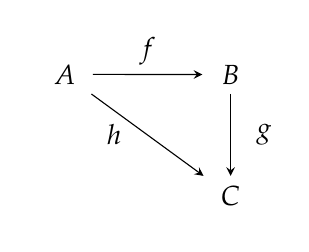
\begin{tikzpicture}
	\matrix (m) [matrix of math nodes,row sep=3em,column sep=4em,minimum width=2em]
	{
	A & B  \\ 
		& C\\};
	\path[-stealth]
		(m-1-1) edge node [above] {$f$} (m-1-2)
	(m-1-1) edge node [left]  {$h~~$} (m-2-2)
	(m-1-2) edge node [right] {$~~g$} (m-2-2);
\end{tikzpicture}
\\ 	
It will be said to \textit{commute} if $h = g\circ f$. The point is that the diagram offers 
two paths from $A$ to $C$, either by composing to follow $f$ and then $g$, or by 
following h directly. Commutativity means that the two paths amount to 
the same thing. A more complex diagram, like the previous one, is said to 
be commutative when all possible triangles that are parts of the diagram 
are themselves commutative. This means that any two paths of arrows in 
the diagram that start at the same object and end at the same object 
compose to give the same over  all arrow. By a \textit{diagram} $D$ in a 
category $\mathscr C$ we simply mean a collection of $\mathscr C$-objects $d_j, d_k,...$ together 
with some $\mathscr C$-arrows $g: d_j \to d_k$ between certain of the objects in the 
diagram. (Possibly more than one arrow between a given pair of objects, 
possibly none). 
A \textit{cone} for diagram $D$ consists of a $\mathscr C$-object $c$ together with a $\mathscr C$-arrow 
$c\to d_j$ for each object $f_j$ in $D$, such that
		\newline
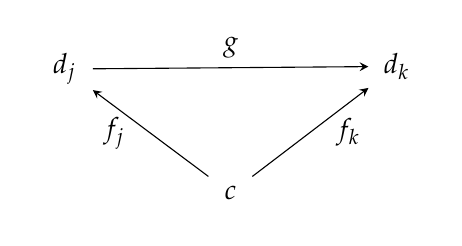
\begin{tikzpicture}
	\matrix (m) [matrix of math nodes,row sep=3em,column sep=4em,minimum width=2em]
	{
	d_j  & & d_k \\ 
		& c  & \\};
	\path[-stealth]
	(m-1-1) edge node [above] {$g$} (m-1-3)
	(m-2-2) edge node [left]  {$f_j~~$} (m-1-1)
	(m-2-2) edge node [right] {$~~f_k$} (m-1-3);
\end{tikzpicture}
\\ 	
 commutes, whenever g is an arrow in the diagram $D$. We use the 
symbolism $\left\{f_j: c\to d_j\right\}$ to denote a cone for $D$. 


A \textit{limit} for a diagram $D$ is a $D$-cone $\left\{f_j: c\to d_j\right\}$ with the property that for 
	any other $D$-cone $\left\{f'_j: c'\to d_j\right\}$ there is exactly one arrow $f:c' \to c$ such 
			\newline
	\begin{tikzpicture}
		\matrix (m) [matrix of math nodes,row sep=3em,column sep=4em,minimum width=2em]
		{
			  & d_j &  \\ 
		c'	&  & c \\};
		\path[-stealth]
		(m-2-1) edge node [above] {$g$} (m-2-3)
		(m-2-1) edge node [left]  {$f'_j~~$} (m-1-2)
		(m-2-3) edge node [right] {$~~f_j$} (m-1-2);
	\end{tikzpicture}
	\\ 	
		commutes for every object $d_j$ in $D$. 
		This limiting cone, when it exists, is said to have the \textit{universal property} 
		with respect to $D$ -cones.
		 A limit for 
		diagram $D$ is unique up to isomorphism.%:- if {ft:  > a\} and {f-:c' > d;} 			are both limits for D, then the unique commuting arrow f: c'  above is 			iso (its inverse is the unique commuting arrow c- *c' whose existence 			follows from the fact that {/,': c'  > dj is a limit). 
		% It is universal amongst such cones-any other 		D-cone factors uniquely through it as in the last diagram.		


\begin{definition}\label{pull_back_defn}\cite{goldblatt:topoi}
	A \textit{pullback} of a pair $a \xrightarrow{f}c \xleftarrow{g} b$ of $\mathscr C$-arrows with a common codomain 
	is a limit in $\mathscr C$ for the diagram 
			\newline
\begin{tikzpicture}
	\matrix (m) [matrix of math nodes,row sep=3em,column sep=4em,minimum width=2em]
	{
		& b  \\ 
		a	&  c \\};
	\path[-stealth]
	(m-1-2) edge node [right]  {$g$} (m-2-2)
	(m-2-1) edge node [above] {$f$} (m-2-2);
\end{tikzpicture}
\\ 	
	
\end{definition}
\section{Functors}
\begin{definition}\label{functor_defn}\cite{goldblatt:topoi}
A \textit{functor} $F$ from category $\mathscr{C}$ to category $\mathscr{D}$ is a function that assigns 
\begin{enumerate}
	\item [(i)]
 to each $\mathscr{C}$-object $a$, a $\mathscr{D}$-object $F(a)$; 
\item[(ii)] to each $\mathscr{C}$-arrow $f:a \to b$ a $\mathscr{D}$-arrow $F(f): F(a) \to F(b)$, 
such that 
\begin{enumerate}
	\item[(a)]  $F\left(\mathbb 1_a\right) = \mathbb 1_{F\left(a\right)}$ for all  $\mathscr{C}$-objects $a$, i.e. the identity arrow on $a$ is assigned 
	the identity on $F\left(a\right)$,
	\item[(b)]  $F\left(g\circ f\right)=F\left(g\right)\circ F\left( f\right) $, whenever $g \circ f$ is defined. 
	This last condition states that the $F$-image of a composite of two arrows 
	is the composite of their $F$-images.
\end{enumerate}


\end{enumerate}
 We write $F:\mathscr{C}\to \mathscr{D}$ or  $\mathscr{C}\xrightarrow{F} \mathscr{D}$ to indicate that $F$ is a 
functor from $
\mathscr{C}$ to $\mathscr{D}$. Briefly then a functor is a transformation that 
"preserves" dom's, cod's, identities and composites. 
\end{definition}
If $a$ and $b$ are  $\mathscr{C}$-objects then a functor $\mathscr{C}\xrightarrow{F} \mathscr{D}$ yields a map
\be\label{f_ab_funct_eqn}
F_{a,b}:\mathscr{C}\left(a, b \right)  \to \mathscr{D}\left( F\left(a\right), F\left(b\right)\right)  
\ee
(cf. Notation \eqref{category_not_eqn}).
\begin{definition}\label{funct_full_faithfull_defn}\cite{bass}
A functor $\mathscr{C}\xrightarrow{F} \mathscr{D}$ is said to be \textit{faithful} (resp. \textit{full}) if the given by \eqref{f_ab_funct_eqn} map is injective (resp. surjective).
\end{definition}
\begin{defn}\label{functor_contravariant_defn}
A \textit{contravariant} functor is one that reverses direction by mapping domains 
to codomains and vice versa. 
Thus $\mathscr{C}\xrightarrow{F} \mathscr{D}$ is a contravariant functor if it assigns to $f: a\to b$ an 
arrow $F(f):F(b)\to F(a)$, so that $F\left(\mathbb{1}_a\right)= \mathbb{1}_{F(a)}$ as before, but now 
$$
F\left( g\circ f\right) = F\left( f\right)\circ  F\left( g\right). 
$$
\end{defn}


\begin{definition}\label{exact_functor_defn}
A left/right exact functor is a functor that preserves finite limits/finite colimits.
\end{definition}
\section{Natural transformations}\label{natural_transformation_sec}
\paragraph{}
Here I follow to \cite{goldblatt:topoi}.
Given two categories $\mathscr C$ and $\mathscr D$ we are going to construct a category, 
denoted $\mathrm{Funct}\left(\mathscr C, \mathscr D\right)$, or $\mathscr D^{\mathscr C}$, whose objects are the functors from $\mathscr C$ to $\mathscr D$. 
We need a definition of arrow from one functor to another. Let 
$F: \mathscr C\to \mathscr D$ and $G: \mathscr C\to \mathscr D$ be two functors. For any $\mathscr C$-object $a$ we define a $\mathscr D$-arrow $\tau_a : F\left(a\right)\to  G\left(a\right)$. We require that each  $\mathscr C$-arrow $f: a \to b$  gives rise to a diagram 
	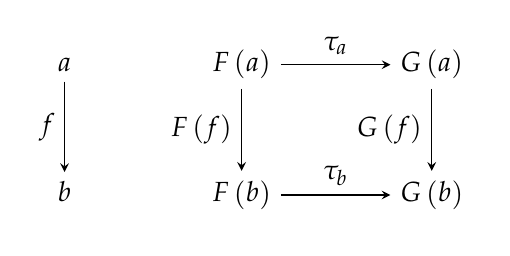
\begin{tikzpicture}
	\matrix (m) [matrix of math nodes,row sep=3em,column sep=4em,minimum width=2em]
	{
	a	& F\left(a \right)  &   G\left(a \right)\\ 
		b	& F\left(b \right)  &   G\left(b \right) \\};
	\path[-stealth]
	(m-1-1) edge node [left]  {$f$} (m-2-1)
	(m-1-2) edge node [above] {$\tau_a$} (m-1-3)
	(m-2-2) edge node [above]  {$\tau_b$} (m-2-3)
	(m-1-2) edge node [left]  {$F\left( f \right)$} (m-2-2)
	(m-1-3) edge node [left]  {$G\left( f \right)$} (m-2-3);
\end{tikzpicture}
\\ 	
that commutes.
%a F(a) Ta > G(a) Ftf)  F(b) T"  G(b) that commutes. Thus  and provide a categorical way of turning the F-picture of f:a-*b into its G-picture. 
In summary then, a \textit{natural transformation} from functor $F: \mathscr C\to \mathscr D$ and $G: \mathscr C\to \mathscr D$  to functor $F: \mathscr C\to \mathscr D$ and $G: \mathscr C\to \mathscr D$  is an assignment $\tau$ that provides, for each $\mathscr C$-object $\mathscr D$-arrow $\tau_a :F(a) \to G(a)$, such that for any $\mathscr C$-arrow $f:a\to b$, the above diagram commutes in $\mathscr D$, i.e. $\tau_b \circ F(f)= G(f)\circ \tau_a$. We use the symbolism $\tau: F\to G$, or $F \xrightarrow{\tau}G$, to denote that $\tau$ is a natural transformation from $F$ to $G$. The arrows $\tau_a$ are called the \textit{components} of $a$. Now if each component $\tau_a$ of $a$ is an iso arrow in $\mathscr D$ then  case we call $\tau$ a \textit{natural isomorphism}. Each $\tau_a: F(a)\to G(a)$ then has an inverse $\tau_a^{-1}: G(a) \to F(a)$, and these $\tau^{-1}_a$'s form the components of a natural isomorphism $\tau^{-1}: G \to F$. We denote natural isomorphism by $\tau: F \cong G$. 
\begin{example}
The identity natural transformation $\mathbb{1}_F :F\to F$ assigns to each object $a$, the identity arrow $\mathbb{1}_{F(a)}:F(a)\to F(a)$. This is clearly a natural isomorphism. 
\end{example}

	\begin{definition}\label{category_equivalence_definition}\cite{goldblatt:topoi}
	A functor $F: \mathscr C\to  \mathscr D$ is called an \textit{equivalence of categories} if there 
	is a functor $G: \mathscr D\to  \mathscr C$ such that there are natural isomorphisms $\tau : 1_{\mathscr C} \cong G \circ F$, and $\sigma : 1_{\mathscr D} \cong F \circ G$, from the identity functor on ${\mathscr C}$ to $ G \circ F$, and 
	from the identity functor on ${\mathscr D}$ to $ F \circ G$.
	
	Categories $\mathscr C$ and $\mathscr D$ are \textit{equivalent},  $\mathscr C$ and $\mathscr D$ when there exists an equivalence $F: \mathscr C\to  \mathscr D$ .
\end{definition}
\begin{definition}\label{natural_defn} 	If $ \A$ is  category then a related to $ \A$ construction is said to be \textit{natural} or \textit{functorial} if it is invariant with respect to isomorphisms of $ \A$.
\end{definition}
	\section{Skeleton and pre-order category}

	\begin{definition}\label{skeletal_defn}\cite{goldblatt:topoi}
		A \textit{skeletal category} is one in which "isomorphic" does actually mean the 
		same as "is", i.e. in which whenever $a\cong b$, then $a=b$. 
	\end{definition}
	\begin{definition}\label{skeleton_defn}\cite{goldblatt:topoi}
		A \textit{skeleton}
		of a category $\mathscr C$ is a full subcategory $\mathscr C_0$ of $\mathscr C$ that is skeletal, and such that each $\mathscr C$-object is isomorphic to one (and only one) $\mathscr C$-object.
	\end{definition}
	\begin{remark}
For any category there is a skeleton.
	\end{remark}
\begin{definition}\label{preordercat_defn}\cite{goldblatt:topoi}
		A category is said to be a \textit{pre-order category} if there is at most one morphism between different objects.
	\end{definition}
	\begin{definition}\label{ord_defn}\cite{goldblatt:topoi}
		A binary relation $R \subset \La\times \La$ on the set $\La$ (writing $pRq$ in place of $\left(p,q \right)\in R$ ) is said to be \textit{pre-ordering} if it is 
		\begin{enumerate}
			\item [(a)] \textit{reflexive}, i.e. for each $p$ we have $pRp$ and
			\item[(b)] \textit{principal !!! \ref{top_principal_defn} !!!}, whenever $pRq$ and $qRs$, we have $pRs$.
		\end{enumerate}
	\end{definition}
	\begin{definition}\label{simply_ord_defn}\cite{goldblatt:topoi}
	A set with $\La$ with pre-ordering $\le$ is \textit{simply ordered} if one has:
	\begin{enumerate}
		\item [(a)] if $\mu, \nu \in \La$ are such that $\mu \le \mu$ and $\nu \le \mu$ then $\mu = \nu$,
		\item [(b)] if $\mu, \nu \in \La$ then $\mu \le \mu$ or/and $\nu \le \mu$.
	\end{enumerate}
	\end{definition}
	\begin{remark}\label{pre_order_rem}\cite{goldblatt:topoi}
		For any set pre-ordered $\La$ with pre-ordering $R$ there is a pre-order category such that
		\begin{enumerate}
			\item [(a)] Objects of the category are elements of $\La$.
			\item[(b)] Morphisms are pairs $\left(p, q \right) \in R$.
			\item[(c)] The composition of morphisms is given by $\left(q,s\right)\circ \left(p, q\right) =\left(p,s\right)$.
		\end{enumerate}
		
	\end{remark}
	\section{Equivalence relations}
	
	\begin{definition}\label{equivalence_relation_defn}\cite{spanier:at}
	An \textit{equivalence relation} in a set $A$ is a relation $\sim$ between elements of $A$ 
	which is \textit{reflexive} (that is, $a\sim a$ for all $a \in A$), \textit{symmetric} (that is, $a\sim a'$ 
	implies $a'\sim a$ for $a, a'\in A$), and \textit{principal !!! \ref{top_principal_defn} !!!} (that is, $a\sim a'$ and $a'\sim a''$
	imply $a \sim a''$ for $a, a', a'' \in A$). The \textit{equivalence class} of $a \in A$ with 
	respect to $\sim$ is the subset $\left\{\left. a'\in A\right| a'\sim a \right\}$. The set of all equivalence classes 
	of elements of $A$ with respect to ~ is denoted by $A/\sim$ and is called a 	\textit{quotient set} of $A$. There is a \textit{projection map} $A \to A/\sim$ which sends $a\in A$ to
	its equivalence class. 
	\end{definition}
	\section{Partially ordered sets}
		\begin{definition}\label{partially_oderedred_set_defn}\cite{johnstone:stone_spaces}
Let $A$ be a set. A {\it partial order} on A is a binary relation $\le$ which 
is 
\begin{enumerate}
	\item[(a)] {\it reflexive}: for all $a \in A$, $a \le a$,
	\item[(b)] {\it transitive}: if $a\le b$ and $b \le c$, then $a\le c$, and 
		\item[(c)] {\it antisymmetric}: if $a \le b$ and $b \le a$, then $a = b$.
\end{enumerate}
 
A {\it poset} (short for {\it partially ordered set}) is a set equipped with a partial 
order. 

\end{definition}
\subsection{Ordinals}
Here the book \cite{harzheim:os} is cited.
A simply ordered set is called \textit{well-ordered}, if each non-empty 
subset of it has a first (or least) element.
We recall in short, without going into the details, the construction of 
the class of ordinal numbers by the method of von Neumann. Consider 
the sequence 
$	\emptyset ,\{\emptyset\},\{\emptyset, \{\emptyset\}\},\{\emptyset, \{\emptyset\}, \{\emptyset, \{\emptyset\}\}\},....$, where from every element x of 
the sequence we create its immediate successor by forming the set $x \cup \{x\}$. 
This step can be repeated transfinitely. The formal definition is: 
A set $M$ whose elements are again sets is called an \textit{ordinal} if there 
holds: $M$, with the relation $\subseteqq$, is well-ordered, and each $x\in M$ is the 
set of all elements of M which are $\subset x$. 
This entails that the class On of all ordinals is well-ordered, and if
$\a$ and $\bt$ are ordinals, we have 
$$
\a < \bt \Leftrightarrow a \text{ is a proper subset of }\bt \Leftrightarrow\a\in \bt.
$$.
The first infinite ordinal is denoted by $\om$ or $\om_0$, and the finite  
ordinals by $0,1,2,...$. 
If $\la$ is an ordinal $\neq \emptyset$, for which the set of ordinals which are $< \la$ has 
no greatest element, then $\la$ is called a \textit{limit ordinal} or \textit{limit number}. If 
this set has a greatest element $\kappa$, $\la$ is said to be a \textit{successor ordinal} or 
\textit{successor number}, and then we also denote $\kappa$ by $\la -1$. 
In On we have operations + and $\bullet$  which can be defined by transfinite 
recursion: 
If $a$ is an ordinal we put $a + 0 = a$ and define $a + 1$ to be the least 
ordinal which is $> a$. If for an ordinal $\bt$ we have already defined $\a +  \bt$
we put $\a + (\bt + 1) = (a + \bt) + 1$.
\begin{thm}\label{zorn_thm}\cite{spanier:at} (Zorn's lemma). A partially ordered set in which every  simply ordered set has an upper bound contains maximal elements.
\end{thm}
\subsection{Ideals and filters}

		\begin{definition}\label{upper_defn}\cite{johnstone:stone_spaces}
Let $A$ be a poset, $S$ a subset of $A$ We say an element $a \in A$
is a {\it join} (or {\it least upper bound}) for $S$, and write $a = \vee S$, if 
\begin{enumerate}
	\item [(a)] a is an upper bound for $S$, i.e. $s \la a$ for all $s \in S$, and 
	\item [(b)] if $b$ satisfies $\forall \in S\quad  s \le b$, then $a \le b$. 
\end{enumerate}
The antisymmetry axiom  ensures that the join of $S$, if it exists, is 
unique. If $S$ is a two-element set $\{s, t\}$, we write $s \vee t$ for $\vee  \{s, t\}$ and if $S$	is the empty set $\emptyset$, we write $0$ for  $\vee \emptyset$.
Similarly we define a  {\it meet} (or {\it greatest lower  bound}) and we use the symbol $\wedge$ for it.
\end{definition}

		\begin{definition}\label{lattice_defn}\cite{johnstone:stone_spaces} 
			
			A \textit{join-semilattice} is a poset which supports for any finite set both  least upper bounds. Similarly we define 	\textit{meet-semilattice},	 A \textit{lattice} is a poset which supports for any finite set both  least upper bounds and greatest lower  bounds. 
			\end{definition}
		\begin{definition}\label{ideal_defn}\cite{johnstone:stone_spaces} 
A subset $I$ of a join-semilattice $A$ is said to be an {\it ideal} if
 \begin{enumerate}
 	\item [(a)] $I$ is a sub-join-semilattice of $A$; i.e. $0\in A$, and $a, b \in I$ imply  	$a \vee b \in I$; and
 	\item [(b)] $I$ is a lower set; i.e. $a \in I$ and $b \le a$ imply $b \in I$.  
 \end{enumerate}
\end{definition}
 		\begin{definition}\label{filter_defn}\cite{johnstone:stone_spaces} 
 	A subset $\mathfrak F$ of a meet-semilattice $A$ is said to be an {\it filter} if
 	\begin{enumerate}
 		\item [(a)] $\mathfrak F$ is a sub-meet-semilattice of $A$; i.e. $1\in A$, and $a, b \in \mathfrak F$  imply  	$a \wedge b \in \mathfrak F$; and
 		\item [(b)] $\mathfrak F$ is a lower set; i.e. $a \in \mathfrak F$ and $ a\le b$ imply $b \in \mathfrak F$.  
 	\end{enumerate}
 \end{definition}
 \begin{empt}\label{filter_empt}
 	Similarly to \cite{bourbaki_sp:gt} we require
 	\begin{enumerate}
 	\item [(c)] $0 \notin \mathfrak F$.
 
 \end{enumerate}	
 \end{empt}
			
		\begin{definition}\label{ultra_filter_defn}\cite{johnstone:stone_spaces} 
A maximal filter is an \textit{ultrafilter}.
\end{definition}

\begin{proposition}\label{top_ultra_thm}\cite{johnstone:stone_spaces}
	One has:
	\begin{enumerate}
		\item [(a)] 	A topological space $\sX$ is Hausdorff if and only if every ultrafilter on $\sX$ has at most one limit.
		\item[(b)]   	A topological space $\sX$ is compact if and only if every ultrafilter has at least one limit.
	\end{enumerate} 

	\end{proposition}
\begin{rem}
	From the Zorn's lemma (cf. Theorem \ref{zorn_thm}) it follows that any filter is a subset of an ultrafilter.
	\end{rem}
	\section{Directed sets}
	
		\begin{definition}\label{directed_set_defn}\cite{engelking:general_topology}
		Let $\La$ be a set and $\le$ is relation on $\La$. We say that $\le$ \textit{directs} $\La$ or $\La$ is \textit{directed} by $\le$, if $\le$ has following properties:
		\begin{enumerate}
			\item [(a)] If $\la \le \mu$ and $\mu \le \nu$, then $\la \le \nu$,
			\item[(b)] For every $\la \in \La$, $\la \le \la$,
			\item[(c)] For any $\mu,\nu \in \La$ there exists a $\la \in \La$ such that $\mu \le \la$ and $\nu \le \la$.
		\end{enumerate}
	\end{definition}
	\begin{definition}\label{cofinal_defn}\cite{engelking:general_topology}
		A subset $\Xi \subset \La$ is said to be \textit{cofinal} in $\La$ if for every $\la \in \La$ there is $\chi \in \Xi$ such that $\la \le \chi$. 
	\end{definition}
\section{Inverse systems}
\begin{definition}\label{inverse_limit_defn}\cite{spanier:at}
An \textit{inverse system of sets} $\left\{A_\a, f^\bt_\a\right\}$ consist of a collection of sets $\left\{A_\a\right\}$ indexed by by a directed set $\La = \left\{\a\right\}$ and a collection of functions $f^\bt_\a: A_\bt \to A_\a$ such that
\begin{enumerate}
	\item [(a)] $f^\a_\a = 1_{A_\a}: A_\a\cong A_\a$ for $\a\in\La$
	\item[(b)] $f^\ga_\a = f^\bt_\a \circ f^\ga_\bt : A_\ga \to A_\a$ for $\a \le \bt \le \ga$ in $\La$
\end{enumerate}
The \textit{inverse limit} $\varprojlim A_\a$ is the subset of $\prod A_\a$ consisting of all points $\left\{a_\a\right\}$ such that if $\a\le\bt$, then $a_\a = f^\bt_\a\left( a_\bt\right) $. For each $\a$ there is a map $p_\a: \varprojlim A_\a\to A_\a$, and if $\a \le \bt$, then $p_\a = f^\bt_\a \circ p_\bt$ . 
\end{definition}
\begin{lemma}\label{inv_lim_lem}\cite{spanier:at}
 Given an inverse system of sets  $\left\{A_\a, f^\bt_\a\right\}$ and given a set $B$ and for every $\a\in \La$ function $g_\a: B \to A_\a$ such that $g_\a = f^\bt_\a \circ g_\bt$ if $\a\le\bt$, there is a unique function $g : B \to \varprojlim A_\a$  such that $g_\a = p_\a\circ g$ for all $\a\in \La$. 
\end{lemma}


	\section{Projective systems}\label{proj_sys_sec}
\paragraph*{}
Here I follow to \cite{phillips:inv_lim_app,phillips:inv_lim,spanier:at}.
An \textit{inverse system} (also called a 
\textit{projective system}) of sets consists of a directed set $D$, a set $X_d$ for each $d\in D$
and functions $\pi_{d,e} : X_d \to X_e$ for all $d,e\in D$ with $d\ge e$, satisfying the consistency 
conditions $\pi_{d,e}= \Id{X_d}$ and $\pi_{e,f}\circ \pi_{d,e} = \pi_{d,f}$. The inverse limit (or 
projective limit) of the system $\left\{X_d\right\}$ is a set $X$ together with functions $\ka_d: X \to X_d$
such that $\pi_{d,e}\circ \ka_e = \ka_d$ for $d \ge e$, and satisfying the following universal property: 
given any set $Y$ and functions $\varphi_d : Y \to X_d$ such that $\pi_{d,e}\circ \varphi_{d,e} = \varphi_d$, there is a 
unique function $\phi : Y \to X$ such that $\phi_s = \ka_d\circ \pi$ for all $d$. The inverse limit $X$ 
is denoted by $\varprojlim X_d$, and it is clearly unique up to unique isomorphism. 
The definition of an inverse limit generalizes in an obvious way to any 
category, and it is easily seen that the same construction produces an inverse limit in 
the categories of abelian groups and homomorphisms, topological spaces and continuous 
maps, and topological $*$-algebras over   $\C$ and continuous $*$-homomorphisms. (The product in (*) is given the product topology and the pointwise algebraic operations).

%\section{Sites}

%\begin{definition}\label{site_defn}\cite{goldblatt:topoi}
%A \textit{Grothendieck topology} on a category $\mathscr C$ is an assignment to each $\mathscr C$-object a of a collection $Cov(a)$ of sets of  $\mathscr C$-arrows with codomain $a$, called \textit{covers} of $a$, such that 
%\begin{enumerate}
%	\item  The singleton $\left\{\mathbb{1}_a : a \xrightarrow{\approx}a\right\}\in Cov(a)$.
%	\item  If $\left\{\left.a_x \xrightarrow{f_x} a \right| x\in X\right\}\in Cov(a)$ then $\left\{\left.a^x_y \xrightarrow{f_x\circ f^x_y} a_x \right| x\in Y_x\right\}\in Cov(a)$.
%	\item $\left\{\left. a_x \xrightarrow{f_x} a \right| x\in X\right\}\in Cov(a)$ and $g : b \to a$ is any  $\mathscr C$-arrow then for each for each $x\in X$ the pullback
%			\newline
%	\begin{tikzpicture}
%		\matrix (m) [matrix of math nodes,row sep=3em,column sep=4em,minimum width=2em]
%		{
%			b\times_a a_x & a_x\\ 
%			 a & b\\};
%		\path[-stealth]
%		(m-1-1) edge node [above] {} (m-1-2)
%		(m-2-1) edge node [above]  {$g$} (m-2-2)
%		(m-1-1) edge node [right]  {$g_x$} (m-2-1)
%		(m-1-2) edge node [right] {$f_x$} (m-2-2);
%	\end{tikzpicture}
%	\\
%		of $f_x$ along $g$ exists, and 	$\left\{\left.	b\times_a a_x \xrightarrow{g_x} b \right| x\in X\right\}\in Cov(b)$.
%\end{enumerate}
%The pair $\left(\mathscr C, Cov\right)$ of the category $\mathscr C$ with the Grothendieck topology $Cov$ is called a \textit{site}. 

%\end{definition}

%\begin{definition}\label{site_sheaf_defn}\cite{goldblatt:topoi}
%A \textit{stack}, or \textit{presheaf}, of sets over  a category $\mathscr C$ is by definition a contravariant functor $F$ from $\mathscr C$:  to the category of sets. The category $\mathbf{PreSh}\left(\mathscr C \right)$  of all stacks over   $\mathscr C$ is thus equivalent to the topos $\mathbf{PreSh}^{\mathscr C^{\text{op}}}$. If $Cov$ is a Grothendieck topology on  $\mathscr C$, and  $\left\{\left.a_x \xrightarrow{f_x} a \right| x\in X\right\}\in Cov(a)$, let 
%			\newline
%\begin{tikzpicture}
%	\matrix (m) [matrix of math nodes,row sep=3em,column sep=4em,minimum width=2em]
%	{
%		a_x\times_a a_y & a_y\\ 
%		a_x & b\\};
%	\path[-stealth]
%	(m-1-1) edge node [above] {} (m-1-2)
%	(m-2-1) edge node [above]  {$f_y$} (m-2-2)
%	(m-1-1) edge node [right]  {} (m-2-1)
%	(m-1-2) edge node [right] {$f_x$} (m-2-2);
%\end{tikzpicture}
%\\
%be the pullback of $f_x$ and $f_y$, for each $x,y\in X$. If $F$ is a stack over   $\mathscr C$ then $F$ gives rise to the functions $F^x_y  :F(a^x)\to F\left( a_x\times_a a_y\right)$  and $F^y_x  :F(a^x)\to F\left( a_x\times_a a_y\right)$ as the $F$-images of the two new arrows obtained by forming this pullback. We denote also by $F_x$ the arrow $F(f_x): F(a) \to  F(a_x)$. A stack $F$ is a \textit{sheaf} over   the site $\left(\mathscr C, Cov\right)$ if and only if it satisfies to the following condition.Given any cover   $\left\{\left.a_x \xrightarrow{f_x} a \right| x\in X\right\}\in Cov(a)$ of a $\mathscr C$-object $a$, and any selection of elements $s_x \in F\left(a_x \right)$ , for all $x\in X$, that are pairwise compatible, i.e. $F^x_y(s_x) = F^y_x(s_y)$ all $x, y\in X$, then there is exactly one $s \in F\left(a\right)$ such that $F_x\left(s \right) = s_x$ for all $x \in X$. The full subcategory of $\mathbf{PreSh}\left(\mathscr C \right)$ generated by those objects that are sheaves over   the site $\left(\mathscr C, Cov\right)$ will be denoted $\mathbf{Sh}\left(Cov \right)$. There is a natural forgetful functor $\mathfrak{Forget} : \mathbf{Sh}\left(Cov \right)\to \mathbf{PreSh}\left(Cov \right)$
%\end{definition}




\chapter{Topology}
	
	
	\section{General topology}
	\begin{definition}\label{top_base_defn}\cite{munkres:topology}
		If $\sX$ is a set, a \textit{basis} for a topology on $\sX$ is a collection $\mathscr B$ of subsets of $\sX$
		(called \textit{basis elements}) such that:
		\begin{enumerate}
			\item [(a)]  for each $x\in \sX$, there is at least one basis element $B$ containing $x$,
			\item [(b)]  if $x$ belongs to the intersection of two basis elements $B_1$ and $B_2$, then there is a
			basis element $B_3$ containing $x$ such that $B_3 \subset B_1\cap B_2$.
		\end{enumerate}
		
		If  $\mathscr B$ satisfies these two conditions, then we define the \textit{topology}  $\mathscr T$ \textit{generated by}  $\mathscr B$ as
		follows: A subset $\sU$ of $\sX$ is said to be \textit{open} in $\sX$ (that is, to be an element of $\mathscr T$) if for
		each $x \in \sU$, there is a basis element $B \in \mathscr B$ such that $x \in B$ and $B \subset \sU$.
	\end{definition}
	\begin{remark}\label{top_base_rem}It is proven that given by the Definition \ref{top_base_defn} collection $\mathscr T$ is a topology  (cf. \cite{munkres:topology}).
	\end{remark}
	\begin{proposition}\label{top_final_prop}\cite{bourbaki_sp:gt}
Let $\sX$ be a set, let $\left\{\sY_\iota\right\}_{\iota\in I}$ be a family of topological spaces, and for each $\iota\in I$ let $f_\iota$ be a mapping of $\sY_\iota$ into $\sX$. Let $\mathfrak{D}$ be a set of subsets $\sU$ of $\sX$ such that $f_\iota^{-1} \left(\sU \right)$ is open in $\sY_\iota$ for each $\iota \in I$; then  $\mathfrak{D}$ is a set of open sets in a topology $\mathfrak{T}$. In particular $\mathfrak{T}$ is the finest topology for which the mappings $f_\iota$ are continuous. In other words, if $g$ is mapping on $\sX$ into a topological space $\sZ$, then $g$ is continuous ($\sX$ carrying the topology $\mathfrak{T}$) if and only if each of the mappings $g\circ f_\iota$ is continuous.
	\end{proposition}
	\begin{definition}\label{top_final_defn}
	Under the hypotheses of Proposition \ref{top_final_prop} we say that the topology $\mathfrak{T}$ is \textit{final} (\textit{with respect to the family of maps} $\left\{f_\iota:\sY_\iota \to \sX\right\}_{\iota\in I}$).
	\end{definition}
		\begin{remark}
		The Definition \ref{top_final_defn} is a specialization of final object (cf. Definition \ref{terminal_object_defn}).
	\end{remark}
	\begin{corollary}\label{top_final_cor}
	Under the hypothesis of the Proposition \ref{top_final_prop} a subset $\sV$ of $\sX$ is closed in the topology  $\mathfrak{T}$ if and only if $f^{-1}\left(\sV \right)$ is closed in $\sY_\iota$ for each $\iota \in I$. 
	\end{corollary}
	\begin{proposition}\label{top_init_prop}\cite{bourbaki_sp:gt}
	Let $\sX$ be a set, let $\left\{\sY_\iota\right\}_{\iota \in I}$ be a family of topological spaces, and for each $\iota \in I$ let $f_\iota$ be a mapping of $\sX$ into $\sY_\iota$.  Let $\mathfrak{S}$ be the set of subsets of $\sX$ of the form $f^{=1}_\iota\left(\sU_\iota \right)$ where $\iota \in I$, $\sU_\iota$ is open in $\sY_\iota$. Let $\mathfrak B$ be the set of finite intersections of sets of $\mathfrak S$. Then $\mathfrak B$ is a base of a topology $\mathfrak T$ and in particular is the coarsest topology on $\sX$ for which the mappings $f_\iota$ are continuous. More precisely of $g$ is a mapping of topological space into $\sY$, then is continuous at a point  $z \in \sZ$ ($\sX$ carrying the topology $\mathfrak T$) if and only if for each of the functions $f_\iota\circ g$ is continuous at $z$.
	\end{proposition}
			\begin{remark}
		The Definition \ref{top_init_prop} is a specialization of initial object (cf. Definition \ref{init_ob_defn}).
	\end{remark}
	
	\begin{definition}\label{top_pointed_defn}
		If $\sX$ is a set (resp. topological space) and $x_0 \in \sX$ is a point then we say that the pair $\left(\sX, x_0 \right)$ is a \textit{pointed  set} (resp. \textit{pointed space}) (cf. \cite{spanier:at,switzer:at}). If both $\left(\sX, x_0 \right)$ and $\left(\sY, y_0 \right)$ are  pointed  spaces and $\varphi: \sX \to \sY$ is such that $\varphi\left(x_0\right)= y_0$ then we say that $\varphi$ is a \textit{pointed map}. We write
		\be\label{top_pointed_eqn}
		\varphi: \left(\sX, x_0 \right)\to\left(\sY, y_0 \right).
		\ee
		We say that $x_0$ is the \textit{base}-\textit{point}.
	\end{definition}
\begin{definition}\label{top_hausdorff_defn}\cite{munkres:topology}
	A topological space $\sX$ is called a Hausdorff space if for each pair $x_1, x_2$
	of distinct points of $\sX$, there exist neighbourhoods $\sU_1$, and $\sU_2$ of $x_1$ and , respectively,
	that are disjoint.
\end{definition}	
\begin{definition}\label{top_connected_defn}\cite{munkres:topology}
Let $\sX$ be a topological space. A \textit{separation} of $\sX$ is a pair $\sU$, $\sV$ of disjoint
nonempty open subsets of $\sX$ whose union is $\sX$. The space  $\sX$ is said to be \textit{connected}
if there does not exist a separation of  $\sX$.
\end{definition}
\begin{remark}\label{top_connected_rem}\cite{munkres:topology}
A space $\sX$ is connected if and only if the only subsets of $\sX$ that are both
open and closed in $\sX$ are the empty set and $\sX$ itself.
\end{remark}
\begin{theorem}\label{top_connected_closure_thm}\cite{munkres:topology}
%Theorem 23.4. 
Let $A$ be a connected subspace of $\sX$, and let $\overline A$ be the closure of $A$, i.e. intersection of containing $A$ closed sets. If $A \subset B \subset \overline A$, then $B$ is also
connected.
\end{theorem}
\begin{definition}\label{top_path_connected_defn}\cite{munkres:topology}
%Definition. 
Given points $x$ and $y$ of the space $\sX$, a \textit{path} in $\sX$ from $x$ to $y$ is a continuous map $f: \left[a, b\right]\to \sX$ of some closed interval in the real line into $\sX$, such
that $f(a) = x$ and $f(b) = y$. A space $\sX$ is said to be \textit{path connected} if every pair of
points of $\sX$ can be joined by a path in $\sX$.
\end{definition}

\begin{definition}\label{top_connected_component_defn}\cite{munkres:topology}
	Given $\sX$, define an equivalence relation on $\sX$ by setting $x\sim y$ if there
	is a connected subspace of $\sX$ containing both $x$ and $y$. The equivalence classes are
	called the \textit{components} (or the \textit{connected components}) of $\sX$.
\end{definition}


\begin{theorem}\label{top_conn_comp_thm}\cite{munkres:topology}
	%Theorem 25.1. 
	The components of $\sX$ are connected disjoint subspaces of $\sX$ whose
	union is  $\sX$, such that each nonempty connected subspace of  $\sX$ intersects only one of
	them.
\end{theorem}
	\begin{definition}\label{top_locally_connected_defn}\cite{munkres:topology}.
	A space $\mathcal X$ is said to be \textit{locally connected at} $x$ if for every neighbourhood $\mathcal U$ of $x$ there is a connected neighbourhood $\mathcal V$ of $x$  contained in $\mathcal U$. If $\mathcal X$ is locally connected at each of its points, it is said simply to be \textit{locally connected}.
\end{definition}
\begin{theorem}\label{top_loc_conn_thm}\cite{munkres:topology}
	A space $\mathcal X$ is locally connected if and only if for every open set $\mathcal U$, each component of $\mathcal U$ is open in $\mathcal X$.
\end{theorem}
\begin{proposition}\label{top_quasi_component_prop}\cite{bredon:topology_geometry}
%	4.11. 	Proposition. 
The statement "$d(p) = d(q)$" for every discrete valued map $d$
	on $\sX$" is an equivalence relation. 
\end{proposition}
\begin{definition}\label{top_quasi_component_defn}\cite{bredon:topology_geometry}
%4.12. Definition. 
The equivalence classes of the relation in Proposition \ref{top_quasi_component_prop}
are called the \textit{quasi}-\textit{components} of $\sX$.
\end{definition}
\begin{proposition}\label{top_quasi_component_closed_prop}\cite{bredon:topology_geometry}
%4.13. Proposition. 
Quasi-components of a space $\sX$ are closed. Each connected
set is contained in a quasi-component. (In particular, each connected component is contained
in a quasi-component.) Quasi-components are either equal or disjoint,
and fill out $\sX$.
\end{proposition}

\begin{exercise}\label{top_loc_conn_exer}\cite{bredon:topology_geometry}
Prove that If $\sX$ is locally connected, show that its components are open and equal its
quasi-components.
\end{exercise}

\begin{definition}\cite{spanier:at}
Given a set $\sX$ and an indexed collection of topological spaces $\left\{\sX_j\right\}_{j \in J}$ functions $f_j : \sX \to \sX_j$, the \textit{topology induced} on $\sX$ by the functions $\left\{f_j\right\}$ is the 
smallest or coarsest topology such that each $f_j$ is continuous. 
\end{definition}

\begin{definition}\label{top_inverse_limit_defn}\cite{spanier:at}
If $\left\{\sX_\a\right\}_{\a\in\La}$ is an inverse system of topological 
spaces (that is, $\sX_\a$ is a topological space for $\a\in \La$ and $f^\bt_\a: \sX_\bt\to \sX_\a$ is  
continuous for $\a\le\bt$) their \textit{inverse limit} $\varprojlim \sX_\a$ (cf. Definition \ref{inverse_limit_defn}) is given the topology induced by the functions $p_\a : \varprojlim \sX_\a\to\sX_\a$  for $\a\in\La$. 
\end{definition}
\begin{definition}\label{top_cover_defn}\cite{munkres:topology}
A collection $\A$ of subsets of a space $\sX$ is said to \textit{cover} $\sX$, or to be a
\textit{covering} of $\sX$, if the union of the elements of $\A$ is equal to $\sX$. 
It is called an \textit{open
covering} of $\sX$ if its elements are open subsets of $\sX$.
\end{definition}

\begin{definition}\label{top_compact_defn}\cite{munkres:topology}
A space $\sX$ is said to be \textit{compact} if every open covering $\A$ of $\sX$ contains
a finite subcollection that also covers $\sX$.
\end{definition}	
	\begin{theorem}\label{top_compact_img_thm}\cite{munkres:topology}
	%	Theorem 26.5. 
	The image of a compact space under a continuous map is compact.
\end{theorem}	

\begin{definition}\label{top_locally_compact_defn}
	A space $\sX$ is said to be \textit{locally compact} at $x$ if there is some compact
	subspace $\sV$  of $\sX$ that contains a neighbourhood of $x$. If $\sX$ is locally compact at each of
	its points, $\sX$ is said simply to be \textit{locally compact}.
\end{definition}
\begin{empt}\cite{engelking:general_topology}
		Every set of cardinal numbers being well-ordered by $<$, the set of all cardinal numbers
		of the form $\left|B\right|$, where $B$ is a base for a topological space $\sX$, has a smallest element; this cardinal number is called the \textit{weight of the topological space} $\sX$ and is denoted by $w\left(\sX\right)$.
		
	\end{empt}

	\begin{theorem}\label{top_weght_thm}\cite{engelking:general_topology}
		%3.4.16. THEOREM. 
		If the weight of both $\sX$ and $\sX$ is not larger than $\mathfrak{m} \ge \aleph_0$ and $\sY$ is a locally
		compact space, then the weight of the space $\sY^\sX$ with the compact-open topology (cf. \ref{top_comp_open_empt})  is not larger
		than $\mathfrak{m}$.
	\end{theorem}	
	
\begin{definition}\label{top_net_defn}\cite{engelking:general_topology}
		A \textit{net in topological space} $\mathcal{ X}$ is an arbitrary function from a non-empty directed set $\La$ (cf. Definition \ref{directed_set_defn}) to the space $\mathcal{ X}$. Nets will be denoted by $S = \left\{x_\la \in \mathcal{ X}\right\}_{\la \in \La}$. 
	\end{definition}
	\begin{definition}\label{top_net_lim_defn}\cite{engelking:general_topology}
		A point $ x \in \mathcal{ X}$ is called a \textit{limit of a net} $S = \left\{x_\la \in \mathcal{ X}\right\}_{\la \in \La}$ if for every neighbourhood $\mathcal U$ of $x$  there exists $\la_0 \in \La$ such that $x_\la \in \mathcal U$ for every $\la \ge \la_0$; we say that $\left\{x_\la \right\}$ \textit{converges} to $x$. The limit will be denoted by $x = \lim S$, or $x = \lim_{\la \in \La} x_\la$, or $\lim x_\la$.
	\end{definition}
	\begin{remark}
		A net can converge to many points, however if $\mathcal{ X}$ is Hausdorff then the net can have the unique limit.
	\end{remark}
	\begin{definition}\label{haudorff_defn}\cite{munkres:topology}
		A topological space $\sX$ is called a \textit{Hausdorff space} if for each pair $x_1$, $x_2$ of distinct points of $\sX$, there exist neighbourhoods $\sU_1$, and $\sU_2$ of $x_1$  and $x_2$, respectively, that are disjoint.
	\end{definition}
	% \begin{definition}\cite{munkres:topology}
	%If a space $\sX$ has a countable basis for its topology, then $\sX$ is said to satisfy the \textit{second countability axiom}, or to be \textit{second-countable ???}.
	% \end{definition}
	\begin{definition}\label{top_normal_defn}\cite{munkres:topology}
		Suppose that one-point sets are closed in $\sX$. Then $\sX$ is said to be  
		\textit{regular} if for each pair consisting of a point $x$ and a closed set $B$ disjoint from $x$, there
		exist disjoint open sets containing $x$ and $B$ respectively. The space $\sX$ is said to be
		\textit{normal} if for each pair $A$, $B$ of disjoint closed sets of $\sX$ there exist disjoint open sets containing $A$ and $B$ respectively.
	\end{definition}
	\begin{definition}\label{top_completely_regular_defn}\cite{munkres:topology}
		A topological space $\mathcal X$ is \textit{completely regular} if one-point sets are closed in  $\mathcal X$ and for each point $x_0$ and each closed $\mathcal \sY \subset \mathcal X$ not containing $x_0$, there is a continuous function $f: \mathcal X \to \left[0,1 \right]$ such that $f\left(x_0 \right)= 1$ and $f\left(\mathcal Y \right)= \left\{0\right\} $.  
	\end{definition}
	\begin{theorem}\label{top_sc_regular_normal_thm}\cite{munkres:topology}
		%Theorem 32.1. 
		Every regular space with a countable basis is normal.
	\end{theorem}
	\begin{exercise}\label{top_completely_regular_exer}\cite{munkres:topology}
		Show that every locally compact, Hausdorff space is completely regular.
	\end{exercise}
	%	\begin{theorem}\label{top_cr_thm}\cite{munkres:topology}
	% 		A subspace of a completely regular space is completely regular. A product of completely regular spaces is completely regular. 
	% 	\end{theorem}
	%	\begin{thm}\label{metr_normal}\cite{munkres:topology}
	% 		Every metrizable space is normal.
	% 	\end{thm}
	
	\begin{thm}\label{comp_normal_thm}\cite{munkres:topology}
		Every compact Hausdorff space is normal.
	\end{thm}
	
	%\begin{thm}\cite{munkres:topology}\label{urysohn_metr_lem}\textbf{ Urysohn metrization theorem.}
	%	Every regular space with a countable  basis is metrizable.
	%\end{thm}
	
	\begin{thm}\label{urysohn_lem}\cite{munkres:topology}\textbf{ Urysohn lemma.}
		Let $\mathcal X$ be a normal space, let $\mathcal A$, $\mathcal B$ be disconnected closed subsets of $\mathcal X$. Let $\left[a,b\right]$ be a closed interval in the real line. Then there exist a continuous map $f: \mathcal X \to \left[a, b\right]$ such that $f(\mathcal A)=\{a\}$ and $f(\mathcal B)=\{b\}$.
	\end{thm}
	\begin{theorem}\label{tietze_ext_thm}\cite{munkres:topology} \textbf{Tietze extension theorem.} Let  $\mathcal X$ be a normal space; let  $\mathcal A$ be a closed subspace of  $\mathcal X$.
		\begin{enumerate}
			\item [(a)] Any continuous map of  $\mathcal A$ into the closed interval $[a,b]$ of $\R$ may be extended to a continuous map of all  $\mathcal X$ into $[a,b]$
			\item [(b)] Any continuous map of  $\mathcal A$ into $\R$ may be extended to a continuous map of all  $\mathcal X$ into $\R$.
		\end{enumerate}
		
	\end{theorem}
\begin{definition}\label{top_onen_map_defn}\cite{munkres:topology}
A map $f: \sX \to \sY$ is said to be an \textit{open map} if for every open set $\sU$ of $\sX$, the
set $f\left(\sU \right)$  is open in $\sY$.
\end{definition}	
	\begin{definition}\label{top_bicont_defn}\cite{kurat:topI}
A continuous map 	 	$f$ is called \textit{bicontinuous} if it is onto and if
	 $$
 \left(A \text{ is open}\right) \Leftrightarrow  \left(f^{-1}\left( A\right)  \text{ is open}\right)
	 $$
	 Equivalently 
	 $$
	 \left(A \text{ is closed}\right) \Leftrightarrow  \left(f^{-1}\left( A\right)  \text{ is closed}\right).
	 $$	
	 \end{definition}
	 \begin{theorem}\label{top_bicont_oc_thm}\cite{kurat:topI}
	Let $f: \sX \to \sY$ be open or closed onto. Then $f$ is bicontinuous.
\end{theorem}
	 \begin{theorem}\label{top_bicont_thm}\cite{kurat:topI}
	 If $f$ is bicontinuous and one-to-one, then $f$ is a homeomorphism.
	 \end{theorem}
	 	 \begin{theorem}\label{top_bicont_inv_thm}\cite{kurat:topI}
	 	If $f$ is bicontinuous and $g: \sY \to \sZ$. If $h \bydef g \circ f$ is continuous, then so is $g$. If $h$ is bicontinuous, then so is $g$.
	 	\newline
	 	\begin{tikzcd}
	 		\sX \arrow[rd, "h"] \arrow[r, "f"]
	 		& \sY\arrow[d, "g"]\\
	 		& \sZ
	 	\end{tikzcd}
	 \end{theorem}
	 
	 \begin{definition}\label{top_separable_defn}\cite{munkres:topology}
	 A space having a countable  dense subset is said to be \textit{separable}.
	 \end{definition}	
	\begin{defn}\label{top_support_defn}\cite{munkres:topology}
		If $\phi: \mathcal X \to \mathbb{C}$  is continuous then the \textit{support} of $\phi$ is defined to be the closure of the set $\phi^{-1}\left(\mathbb{\C}\setminus \{0\}\right)$ Thus if $x$ lies outside the support, there is some neighbourhood of $x$ on which $\phi$ vanishes. Denote by $\supp \phi$ the support of $\phi$.
	\end{defn}
%	 	\begin{thm}\label{comm_sep_thm}\cite{chun-yen:separability}
%	 		For a locally compact Hausdorff space $\mathcal X$, the following are 		equivalent:
%	 		\begin{enumerate}
%				\item[(a)] The Abelian $C^*$-algebra $C_0\left(\mathcal X \right)$  is separable;
%	 			\item[(b)]$\mathcal X$ is $\sigma$-compact and metrizable;
%				\item[(c)]$\mathcal X$ is second-countable.
%			\end{enumerate}
%		\end{thm}
	%	\begin{thm}\label{top_sec_cov_thm}\cite{munkres:topology}
	%		Suppose that $\mathcal X$ is second-countable space. Then:
	%		\begin{enumerate}
	%			\item[(a)]  Every open covering contains a countable  collection covering $\mathcal X$.
	%			\item[(b)] There exists a countable  subset of $\mathcal X$  which is dense in $\mathcal X$.
	%		\end{enumerate}
	%	\end{thm}
	%\subsection{Locally compact spaces}
	
	
	There are two equivalent definitions of $C_0\left(\mathcal{X}\right)$ and both of them are used in this book.
	\begin{defn}\label{c_c_closure_defn}\cite{murphy}
		An algebra $C_0\left(\mathcal{X}\right)$ is the $C^*$-norm closure of the algebra $C_c\left(\mathcal{X}\right)$ of compactly supported continuous complex-valued functions.
	\end{defn}
	\begin{defn}
		\label{c_c_compact_defn}\cite{blackadar:ko,murphy}
		A $C^*$-algebra $C_0\left(\mathcal{X}\right)$ is given by the following equation
	\bean
			C_0\left(\mathcal{X}\right) \ \left\{\varphi \in C_b\left(\mathcal{X}\right) \ | \ \forall \varepsilon > 0 \ \ \exists K \subset \mathcal{X} \ ( K \text{ is compact}) \ \& \ \forall x \in \mathcal X \setminus K \ \left|\varphi\left(x\right)\right| < \varepsilon  \right\},
		\eean
		i.e.
		\begin{equation*}
			\left\|\varphi|_{\mathcal X \setminus K}\right\| < \varepsilon.
		\end{equation*}
	\end{defn}
	\begin{definition}\label{top_ind_lim_defn}\cite{candel:foliII,MW08}

	Let $\sX$ be a locally compact Hausdorff space, and let $C_c\left(\sX\right)$ denote the	space of continuous, compactly supported functions on $\sX$. The natural	topology on $C_c\left(\sX\right)$ is the \textit{inductive limit topology}, defined as follows. A net	$\left\{f_\a\right\}$ in $C_c\left(\sX\right)$ converges to $f$ if there is a compact set $K\subset\sX$ containing	the supports of all $f_\a$ and $f$, and such that $f_\a$ converges uniformly to $f$ on$K$.
	\end{definition}
	\begin{defn}\label{top_loc_fin_defn}\cite{munkres:topology}
		An indexed family of sets $\left\{A_\al\right\}$ of topological space $\sX$ is said to be \textit{locally finite} if each point $x$ in $\sX$  has a neighbourhood that intersects for only finite many values of $\a$.
	\end{defn}
	\begin{defn}\label{top_part_of_unity_defn}\cite{munkres:topology}
		Let $\left\{\mathcal U_\alpha\in \mathcal X\right\}_{\alpha \in \mathscr A}$ be an indexed open covering of $\mathcal{X}$. An indexed family of functions 
		\begin{equation*}
			\phi_\alpha : \mathcal X \to \left[0,1\right]
		\end{equation*}
		is said to be a {\it partition of unity }, dominated by $\left\{\mathcal{U}_\alpha \right\}$, if:
		\begin{enumerate}
			\item $\phi_\alpha\left(\mathcal X \setminus \mathcal U_\alpha\right)= \{0\}$
			\item The family $\supp\phi_\alpha$ is locally finite.
			\item $\sum_{\alpha \in \mathscr A}\phi_\alpha\left(x\right)=1$ for any $x \in \mathcal X$.
		\end{enumerate}
	\end{defn}
 \begin{definition}\label{top_paracompact_defn}\cite{munkres:topology}
	A space $\sX$ is \textit{paracompact} if every open covering $\sX = \cup~\sU_{   \a}$ has a locally finite open refinement $\sX = \cup~\sV_{   \bt}$.
\end{definition}	
\begin{thm}\label{top_part_u_thm}\cite{munkres:topology}
	Let $\mathcal X$ be a paracompact Hausdorff space; let $\left\{\mathcal U_\alpha\in \mathcal X\right\}_{\alpha \in \mathscr A}$ be an indexed open covering of $\mathcal{X}$. Then there exists a partition of unity, dominated by $\left\{\mathcal{U}_\alpha \right\}$.  
\end{thm}

	\begin{prop}\label{top_smooth_part_unity_prop} \cite{brickell_clark:diff_m}
		A differential manifold $M$ admits a (smooth) partition of unity if and only if it is paracompact. 
	\end{prop}
	%\begin{theorem}\label{top_paracompact_norm_thm}
	%	Theorem 41.1. 
	%Every paracompact Hausdorff space $\sX$ is normal
	%\end{theorem}
	%\begin{defn}
	%	A space for which every open covering contains a countable  subcovering is called a \textit{Lindel\"{o}f space}.
%	\end{defn}
	\begin{defn}\label{lindel_defn}\cite{engelking:general_topology}
	 We say that a topological space $\sX$ is a \textit{Lindel\"{o}f space}, or has  a \textit{Lindel\"{o}f property}, if $\sX$ is regular and every open covering  of $\sX$ contains a countable !!! subcovering. 
	 \end{defn}
	\begin{theorem}\label{lindel_thm}\cite{engelking:general_topology}
	Every regular second-countable  space in Lindel\"{o}f.
	\end{theorem}
	\begin{theorem}\label{lindel_para_thm}\cite{munkres:topology}
		%Theorem 41.5. 
		Every regular Lindel\"{o}f space is paracompact.
	\end{theorem}
	\begin{definition}\label{top_compactification_defn}\cite{munkres:topology}
		If $\sY$ is a compact Hausdorff space and $\sX$ is a proper subspace of $\sY$ whose
		closure equals $\sY$, then $\sY$ is said to be a \textit{compactification} of $\sX$. If $\sY\setminus\sX$ equals a single
		point, then $\sY$ is called the \textit{one-point compactification} of $\sX$.
	\end{definition}
	\begin{remark}
		It is shown  (cf. \cite{munkres:topology}) that $\sX$ has a one-point compactification $\sY$ if and only if $\sX$ is
		a locally compact Hausdorff space that is not itself compact. We speak of $\sY$ as "the"
		one-point compactification because $\sY$ is uniquely determined up to a homeomorphism.
	\end{remark}
	\begin{theorem}\label{sc_comp_thm}\cite{munkres:topology}
		%Theorem 38.2. 
		Let $\sX$ be a completely regular space. There exists a  
		compactification $\sY$ of $\sX$ having the property that every bounded continuous map $f : \sX\to\R$
		extends uniquely to a continuous map of $\sY$ into $\R$.
	\end{theorem}
	
	\begin{definition}\label{top_stone_cech_defn}\cite{munkres:topology}
		For each completely regular space $\sX$, let us choose, once and for all,
		a compactification of $\sX$ satisfying the extension condition of Theorem \ref{sc_comp_thm}. We will
		denote this compactification of  by $\bt\sX$ and call it the \textit{Stone-\v{C}ech compactification}  
		of $\sX$. It is characterized by the fact that any continuous map $\sX\to\sY$ of $\sX$ into a
		compact Hausdorff space $\sY$ extends uniquely to a continuous map $\bt\sX\to\sY$.
	\end{definition}
\begin{theorem}\label{top_sc_to_compact_thm}\cite{munkres:topology}
%Theorem 38.4. 
Let $\sX$ be a completely regular space; let $\bt\sX$ be the  {Stone-\v{C}ech compactification} of $\sX$. Given any continuous map $f: \sX \to \sY$ into a compact Hausdorff space $\sY$, the map $f$ extends uniquely to a
continuous map $\bt f: \bt \sX\to\sY$.
\end{theorem}	
	
	\begin{definition}\label{f_topology_defn}\cite{rudin:fa}
		Suppose next that $\sX$ is a set and $\mathscr F$ is a nonempty family of mappings $f: \sX \to \sY_f$, where each $\sY_f$ is a topological space. (In many important cases, $\sY_f$ is the same for all $f \in \mathscr F$.) Let $\tau$ be the collection of all unions of finite intersections of sets $f^{-1}\left(\sV  \right)$ with $f\in \mathscr F$ and $\sV$ open in $\sY_f$. Then $\tau$ is a topology on $\sX$, and it is in fact the weakest topology on $\sX$ that makes every 
		$f\in \mathscr F$ continuous: If $\tau'$ is any other topology with that property, then $\tau\subset\tau'$. This $\tau$ is called the \textit{weak topology on} $\sX$ \textit{induced by} $\mathscr F$, or, more 
		shortly, the $\mathscr F$-\textit{topology of} $\sX$.
	\end{definition}
	\begin{definition}\label{top_locally_contractible_defn}\cite{spanier:at,switzer:at}
		A topological space $\sX$ is said to be 
		\textit{contractible} if the identity map of $\sX$ is homotopic to some constant map of $\sX$ 
		to itself. $\sX$ is \textit{locally contractible} if
		every neighbourhood $\sU$ of a point $x$ contains a neighbourhood $\sV$ of $x$ deformable to $x$ in $\sV$). 
		
	\end{definition} 
\begin{definition}\label{top_simply_conn_defn}\cite{spanier:at}
Let $E^{k+1}, S^k\subset\R^{k+1}$ be a disk ans a sphere, i.e.
\bean
E^{k+1} \bydef \left\{\left.\left(x_1, ..., x_{k+1}\right) \in \R^{k+1}~\right| x_1^2+...+x^2_{k+1}\le 1\right\},\\
S^k \bydef \left\{\left.\left(x_1, ..., x_{k+1}\right) \in \R^{k+1}~\right| x_1^2+...+x^2_{k+1}= 1\right\}
\eean
with the natural inclusion $S^k\subset E^{k+1}$. A space $\sX$ is said to be $n$-\textit{connected} if every continuous map $f: S^k \to \sX$ for $k\le n$ has a continuous extension over $E^{k+1}$. A 1-connected space is also said to be \textit{simply connected}.
\end{definition}
	
%\subsection{Moore-Smith convergence}
	\begin{theorem}\label{it_lim_thm}\cite{kelley:gt}
	\textit{Theorem on iterated limits}. Let $D$ be a directed set, let $E_m$ be a directed set for each $m$ in $D$, let $F$ be the product $D\times \prod_{m \in D}  E_m$, and for $(m,f)$ in $F$ let $R(m,f) = (m, f(m))$. If $S(m,n)$ is 
	a member of a topological space for each m in $D$ and each $n$ in $E_n$, 
	then $S\circ R$ converges to $\lim_m \lim_nS(m,n)$ whenever this iterated limit 
	exists.
\end{theorem}
%Let $\sX$ is a set.
%If $\mathcal C$ is a class consisting of pairs $(S,s)$, where $S$ is a net in $\sX$ and $s$ a point, when is there a topology $\mathcal T$ for X such that (6  e C iff S  converges to s relative to the topology 3
\begin{definition}\label{top_lower_semi_defn}\cite{bourbaki_sp:gt}
A real-valued function $f$, defined on a topological space $\sX$, is said to be \textit{lower semi-continuous} (resp. \textit{upper semi-continuous} at point $a \in \sX$ if for each $h < f\left(a\right)$ (resp. each $k > f\left(a\right))$ there is an open neighbourhood $\sV$ of $a$ such that $h < f\left(x\right)$ (resp. each $k > f\left(x\right))$ for each $x\in\sV$.\\
A real-valued function $f$, is said to be \textit{lower semi-continuous} (resp. \textit{upper semi-continuous} on $\sX$ if it is  {lower semi-continuous} (resp. {upper semi-continuous} at every point of $\sX$.
\end{definition}
\begin{theorem}\label{top_lower_semi_thm}\cite{bourbaki_sp:gt}
	Let $f$ be a lower semi-continuous function on a non-empty quasi-compact space $\sX$. Then there is at least one point $a \in \sX$ such that $f\left(a \right) = \inf_{x \in \sX}f\left( x\right) $ (in other words, $f$ attains its greatest lower bound in $\sX$).
\end{theorem}
\begin{remark}\label{top_lower_semi_rem}
There is inverted result about upper semi-continuous functions and supremums.
\end{remark}


\begin{empt}\label{top_cauchy_empt}\cite{engelking:general_topology}
If $\left( \sX, \rho\right) $ is a metric space then wa say that $\left\{x_j\right\}_{j \in \N}\subset \sX$ is a \textit{Cauchy sequence} if for every $\eps > 0$ there exist $k > 0$ such that $\rho\left(x_j, x_k \right) < \eps$ whenever $j> k$. If $\left( \sX, \rho\right)$ is complete then any Cauchy sequence is convergent.
\end{empt}
\begin{remark}\label{top_cauchy_rem}
Above statements can be generalized to nets (cf. Definition \ref{top_net_lim_defn}) the word \textit{Cauchy net} is also used in this book.
\end{remark}
%\begin{defn}\label{top_dfn:regular_neighbourhood_defn}\cite{pavlov_troisky:cov}
	%2.1
%	Let $\sX, \sY$ be Hausdorff spaces, and let $p: \sY \to \sX$ be a continuous map.If 		$x\in \sX$, which has a finite number of pre-images $y_1,		\dots,y_m$. Then a neighbourhood $\sU$ of $x$ is said to be		\emph{regular} if
%		\begin{gather}\label{eq:neiborhoods}
%			p^{-1}(\sU)= \sV_1\sqcup\dots\sqcup \sV_m,
%		\end{gather}
%		where $\sV_i$ are some neighbourhoods of $y_j$, $j=1,\dots, m$.
%\end{defn}

%\begin{lem}\label{top_lem:neiborhoods_lem}\cite{pavlov_troisky:cov}
%	2.2.
%	Let $p : \sY\rightarrow \sX$ be a continuous closed map of Hausdorff	spaces. Then any point $x$ of $\sX$ with a finite number of	pre-images has a regular neighbourhood.
%\end{lem}

\begin{definition}\label{metric_space_defn}\cite{rudin:pa}
	%2.15 Definition
	A set $X$, whose elements we shall call \textit{points}, is said to be a 
	\textit{metric space} if with any two points $p$ and $p$ of $X$ there is associated a real 
	number $(p, q)$, called the \textit{distance} from $p$ to $q$, such that
	\begin{enumerate}
		\item [(a)]
		\bean
		p \neq q \quad \Leftrightarrow \quad d\left(p, q\right)> 0;\\
		d(p,p)=0;
		\eean
		\item[(b)] $d(p,q)=d(q,p);$
		\item[(c)] $\forall r \in X \quad d(p, q) < d(p, r) + d(r, q)$.
	\end{enumerate} 
	Any function with these three properties is called a \textit{distance function}, or a \textit{metric}. 
\end{definition}

\begin{remark}\label{triangle_ineq_rem}
	The condition (b) of the Definition \ref{metric_space_defn} is said to be the \textit{triangle inequality}. If $Y$ is a normed vector space then there is a distance function on $Y$ such that
	$$
	d(x, y)\bydef \left\|x - y \right\| \quad \forall x, y \in Y.
	$$
	The triangle identity is given by
\be\label{triangle_ineq_vec_eqn}
	\forall x, y, z \in Y \quad  \left\|x - y \right\|\le  \left\|x - z \right\|+ \left\|y - z \right\|.
\ee
\end{remark}
\begin{definition}\label{top_order_top_defn}\cite{counter_topology}
	Let $\sX$ be a set which is linearly ordered by the principal  \ref{top_principal_defn}  relation "<". We define the \textit{order (or interval) topology} on $\sX$ by taking as a basis the open intervals
	\be\label{top_order_top_eqn}
	\left(x,y\right)\bydef \left\{x \in \sX| y < x < z\right\}
	\ee 
\end{definition}
\begin{empt}\label{top_lex_square_empt}\cite{counter_topology,munkres:topology}
	Let $I^2_o = \left[0,1\right]^2$ be a unit square. We order $I^2_o$ lexicographically
	\be\label{top_order_top_s_eqn}
	\forall (x, y),(u, w) \in \left[0,1\right]^2 = I^2_o \quad (x, y)< (u, w)  = \begin{cases}
		y < w & x = u\\
		x < u & \text{otherwise}
	\end{cases}
\ee
	and place the order topology on $I^2_o$. It is proven in  \cite{counter_topology,munkres:topology} $I^2_o$ is connected but it is not path connected.
	The space $I^2_o$ is said to be the \textit{the ordered square} (cf. \cite{munkres:topology}).
\end{empt}

\section{Algebraic topology}
\subsection{Exact sequences of sets of homotopy classes}
\paragraph{}
\begin{definition}\label{top_red_cone_defn}\cite{spanier:at}
If $\left(\sX, x_0\right)$ is a pointed space then the \textit{reduced cone} $C\sX$ over   $\sX$ is given by
$$
C\sX \bydef \left( \sX \times \left[0, 1\right]\right) /\left( \{x_0\} \times \left[0, 1\right] \cup \sX \times \{0\}\right) 
$$
We shall use $\left[x, t\right]$ to denote the point of $C\sX$ corresponding to the point 
$\left(x, t \right) \in \sX \times \left[0, 1\right]$. $\sX$ is imbedded as a 
closed subset of $C\sX$ by the map $x \mapsto \left[x, 1\right]$. If $\left(\sX, \sA \right)$ is a pair, then $C\sA$ is a subspace of $C\sX$ and $C\left(\sX, \sA \right)$  is defined to be the pair $\left(C\sX, C\sA\right)$.
\end{definition} 
\begin{lemma}\label{top_red_cone_lem}\cite{spanier:at}
A map $f: \left(\sX, \sA\right) \to \left(\sY, \sB\right)$ is null homotopic if and only if there 
is a map $F: C\left(\sX, \sA\right) \to \left(\sY, \sB\right)$  such that $F\left[x, 1\right]= x$ for all $x \in \sX$ 
\end{lemma}
\begin{definition}\label{top_kernel_defn}\cite{spanier:at}
 Given a map $f:  \left(\sX, \sA\right)\to  \left(\sX', \sA'\right)$, the \textit{kernel} of the induced map
 $$
f_{\#}: \left[ \sX, \sA; \sY, \sB\right]
 $$ 
is defined to be the pointed set $f_{\#}^{-1}\left(0 \right)$  and is denoted by $\ker f_{\#}$. 
We now show how to map another set of homotopy classes into  $\left[ \sX, \sA; \sY, \sB\right]$ so that its image equals $\ker f_{\#}$.
\end{definition}
\begin{definition}\label{top_mapping_cone_defn}\cite{spanier:at}
The \textit{mapping cone} $C_f$ of a map $f : \sX' \to \sX$ is defined 
to be the quotient space of $C\sX' \wedge \sX$ by the identifications $\left[x', 1\right] = f\left( x'\right)$ for all $x' \in \sX'$. Given a map $f: \left(\sX', \sA'\right) \to  \left(\sX, \sA\right)$ there is a functorial imbedding of $\left(\sX, \sA \right)$  as a closed subpair of 
$(C_{f'},C_{f''})$. 
\end{definition}
\begin{definition}\label{top_exact_defn}\cite{spanier:at}
	A three-term sequence of pairs and maps 
	$$
\left(\sX', \sA'\right)\xrightarrow{f}\left(\sX, \sA\right)\xrightarrow{g}\left(\sX'', \sA''\right)
	$$
	is said to be \textit{exact} if for any pair $\left( \sY, \sB\right)$ (where $\sB$ is not necessarily closed in $\sY$) the associated sequence of pointed sets 
	$$
\left[\sY, \sB; \sX', \sA'\right]\xrightarrow{f_{\#}}\left[\sY, \sB; \sX, \sA\right]\xrightarrow{g_{\#}}\left[\sY, \sB; \sX'', \sA''\right]
	$$
	is {exact} (that is, $\ker f_{\#}= \im g_{\#}$)
\end{definition}
\subsection{$H$-groups and $H$-cogroups}
\paragraph{}
Here I follow to \cite{spanier:at}. If both $\sX$ and $\sY$ are topological spaces then we denote by $\left[\sX; \sY\right]$ the set of homotopy classes of continuous maps from $\sX$ to $\sY$. One method of obtaining a group structure on  $\left[\sX; \sY\right]$ is to start with a 
group structure on $\sY$. Thus, let $\sY$ be a topological group with identity element as base point. There is a law of composition in the set of all base-point-preserving continuous maps from $\sX$ to $\sY$ defined by point-wise multiplication 
of functions. That is, if $g_1, g_2: \sX \to\sY$, then $g_1g_2: \sX \to\sY$ is defined by $g_1g_2\left(x\right)\bydef g_1\left(x\right)g_2\left(x\right)$, where the right-hand side is the group product in $\sY$. With 
this law of composition, the set of base-point-preserving continuous maps 
from $\sX$ to $\sY$ is a group (which is Abelian if $\sY$ is Abelian). The law of  
composition carries over   to give an operation on homotopy classes such that $\left[g_1\right]\left[g_2\right]\bydef \left[g_1g_2\right]$, and we have the following theorem. 
\begin{theorem}\label{top_hgr_thm}\cite{spanier:at}
If $\sY$ is a topological group, there is a contravariant functor from 
the homotopy category of  pointed  topological spaces to the category of groups 
and homomorphisms. 
\end{theorem}
\begin{remark}\label{top_hgr_rem}
For any topological group $\sY$ we denote by $\left[~\cdot~;\sY\right]$ the given by the Theorem \ref{top_hgr_thm} functor.
\end{remark}
\begin{definition}
An  $H$ cogroup consists of a pointed topological space $Q$ together with a 
continuous comultiplication
$$
\nu : \Q \to Q\vee Q
$$ 

such that the following properties hold: 
\begin{itemize}
	\item \textit{Existence of homotopy identity}. If $c: Q \to Q$ is the (unique) constant 
	map, each composite 
	$$
Q \xrightarrow{\nu} Q\vee Q\xrightarrow{\left(c, 1 \right) }Q \quad \text{and} \quad Q \xrightarrow{\nu} Q\vee Q\xrightarrow{\left(1, c \right) }Q 
	$$
	is homotopic to $1_Q$.
	\item \textit{Homotopy associativity}. 
	\\
	\begin{tikzcd}
		Q \arrow[r, "\nu"] \arrow[d, "p"]  & Q\vee Q \arrow[d, "1\vee p"] \\
		Q\vee Q \arrow[r, "\nu\vee 1"]& Q\vee Q\vee Q
	\end{tikzcd}
	\\	
	is homotopy commutative. 
	\end{itemize}


\end{definition}

	\subsection{Loop space and suspension in topology}

%	\begin{defn}\label{cov_proj_cov_grp}\cite{spanier:at}
%		Let $p: \tilde{X} \to X$ covering projection.  It is clear that there is a {\it group of self-equivalences} of $p$ (a self-equivalence is a homeomorphism $f:\tilde{X}\to\tilde{X}$ such that $p \circ f = p$). We denote this group by $G(\tilde{X}| X)$. This group is also called the {\it group of covering transformations} of $p$.
%	\end{defn}


\begin{empt}\label{top_comp_open_empt} {\it Function spaces.}\cite{switzer:at} If $\sX$ and $\sY$ are topological spaces, we let $\sY^\sX$ denote the set of all continuous functions functions $f: \sX \to \sY$. We give this set a topology, called the {\it compact-open topology}, by taking as a sub-base for the topology all sets of the form $N_{K,U} =\{f:f(K)\subset \sU\}$, $K\subset \sU$ compact, $\sU \subset \sX$ open. 
\end{empt}
\begin{empt}\label{base_points}\cite{switzer:at} {\it Base points.} \cite{switzer:at} Algebraic topology often have to consider not just topological space $\sX$ but rather a space $\sX$ together with a distinguished point $x_0\in \sX$ called the {\it base point}. The pair $(\sX, x_0)$ is called a {\it  pointed space} (one also speaks of  pointed sets). When we are concerned with  pointed spaces $(\sX, x_0)$, $(\sY, y_0)$, etc. we always require that all functions $f: \sX \to \sY$ shall preserve base point, i.e. $f(x_0)=y_0$, and that all homotopies $F:\sX\times I \to \sY$ be relative to base point, i.e. $F(x_0, t) = y_0$, $\forall t \in I$ unless an explicit disclaimer to be contrary is made. We shall use the notation $[\sX, x_0, \sY, y_0]$ to denote the homotopy classes of base point preserving functions, where homotopies are $\mathrm{rel}x_0$, of course. $[\sX, x_0, \sY, y_0]$ is a  pointed space with base point $f_0$ the constant function: $f_0(x)=y_0$, $\forall x\in \sX$. If $(\sX, x_0)$, $(\sY, y_0)$ are  pointed spaces then we have the space $(\sY, y_0)^{(\sX, x_0)}$ of base point preserving functions. We use the notation $\sX \vee \sY$ for the subspace $\sZ \times \{x_0\} \cup \{z_0\} \sX$. It can be thought of as the result of taking the disjoint union $\sZ \cup \sX$ and identifying $z_0$ with $x_0$, $\sZ \vee \sX$ is again a  pointed space with base point $(z_0, x_0)$.  Given maps $f: (\sX, x_0)\to (\sX', x'_0)$ and $g: (\sY, y_0)\to (\sY', y'_0)$ the map $f \times g : \sX\times \sY \to \sX'\times \sY'$ maps $\sX \vee \sY$ into $\sX' \vee \sY'$ and so induces a map $f \wedge g: \sX\wedge \sY \to \sX'\wedge \sY'$.
\end{empt}
\begin{empt}\label{smash_pointed_sp}
	If both $(\sX, x_0)$, $\left( \sY, y_0\right) $ are  pointed spaces then we define the {\it smash product} $(\sX \wedge \sY, *)$ to be the quotient 
	\begin{equation}\nonumber
		\sX \wedge \sY = \sX \times \sY / \sX \vee \sY
	\end{equation}
	with the point $* = p(\sX\vee \sY)$ as base point. Here $p: \sX \times \sY \to X \vee Y$ is the projection. For any $(x,y)\in \sX \times \sY$ we denote $p(x,y)\in \sX \wedge \sY$ by $[x,y]$.
\end{empt}
\begin{thm}\cite{switzer:at}
	If $(\sX, x_0), (\sY, y_0), (\sZ, z_0)$ are  pointed spaces, $\sX, \sZ$ Hausdorff and $\sZ$ locally compact, then there is a natural equivalence
	\begin{equation}
		A: [\sZ \wedge \sX, *; \sY, y_0] \to [\sX, x_0, (\sY, y_0)^{(\sZ, z_0)}, f_0]
	\end{equation}
	defined by $A[f]=[\hat f]$, where if $f: \sZ \wedge \sX \to \sY$ is a map then $\hat f: \sZ \wedge \sX \to \sY$ is a map given by $(\hat f(x)(z)=f[z,x]$.
\end{thm}
\begin{empt}\label{topological_loop_spaces} \cite{switzer:at} If $(\sY, y_0)$ is a  pointed space, we define the {\it loop space} $(\Omega \sY, \omega_0)$ of $\sY$ to be function space 
	\begin{equation}\nonumber
		(\Omega \sY, \omega_0) = (\sY, y_0)^{(S^1, s_0)}
	\end{equation}
	with constant loop $\omega_0$ $(\omega_0(s))= y_0, \ \forall s \in S^1$ as base point.
\end{empt}
\begin{definition}\label{top_sus_defn}\cite{hatcher:at}
	For a space $\sX$, the \textit{(unreduced) suspension} $\Sigma\sX$ is the quotient of $\sX\times [0,1]$ obtained by collapsing $\sX\times\{0\}$ to one point and  $\sX\times\{1\}$ to another.
	point.
\end{definition}
\begin{empt}\label{topological_suspension}\cite{switzer:at}
	If $(\sX, x_0)$ we define {\it suspension} $(\Sigma \sX, *)$ to be the smash product $(S^1 \wedge \sX, *)$ of $\sX$ with the 1-sphere.
\end{empt}
\begin{cor}\label{loop_susp_adj_cor}\cite{switzer:at}		If both $(\sX, x_0), (\sY, y_0)$ are  pointed spaces and $\sX$ is Hausdorff, then there is a natural equivalence
	\begin{equation}\nonumber
		A:[\Sigma \sX,*;\sY,y_0]\cong [\sX, x_0, \Omega \sY, y_0].
	\end{equation}
\end{cor}
\begin{prop}\label{loop_susp_adj_prop}\cite{switzer:at}
	The adjoint correspondence
	\begin{equation}\nonumber
		A:[\Sigma \sX,*;\sY, y_0]\cong [\sX,x_0, \Omega \sY, \omega_0]
	\end{equation}
	is an isomorphism of groups.
\end{prop}
\begin{remark}\cite{switzer:at}
Both sets $[\Sigma \sX,*;\sY, y_0]$ and $[\sX,x_0, \Omega \sY, \omega_0]$ posses the natural group structure.
\end{remark}

\begin{definition}\label{top_hn_bas_defn}\cite{switzer:at}
	% 2.60 page 34
	For $n\ge1$  we define  $n^{\text{th}}$ \textit{homotopy group} $\pi_n\left(\sX, x_0 \right)$ of $\left(\sX, x_0 \right)$ as 
	$$
	\pi_n\left( \sX, x_0\right) \bydef \pi_0\left( \Om^n\sX, \om_0\right) \cong \pi_1\left( \Om^{n -1}\sX, \om'_0\right).
	$$
	where $\pi_0\left( \Om^n\sX\right) $ is a set of connected components of $\Om^n\sX$,
\end{definition}
\begin{remark}\label{top_homotopy_group_rem}\cite{switzer:at}
The group $\pi_1\left(\sX, x_0 \right)$ is a set of homotopy equivalence classes of closed paths $f: \left[0, 1\right] \to\sX$ such that $f\left(0\right)= f\left(1\right)= x_0$. For all $n \in \N$ there is the natural bijective map $\pi_n\left(\sX, x_0 \right)\cong \left[\sX, x_0; S^n, s_0\right]$. We say that $\pi_1\left(\sX, x_0 \right)$ is the \textit{fundamental group} of the  pointed space $\left(\sX, x_0 \right)$. 
\end{remark}

	\begin{defn}\label{top_semi1_defn}\cite{spanier:at}
	A space $\sX$ is said to by \textit{semilocally} 1-\textit{connected} if every point $x_0$ has a neighbourhood $N$ such that $\pi_1\left( N, x_0\right) \to \pi_1\left(\sX, x_0 \right)$ is trivial. 
\end{defn} 

\begin{remark}\cite{switzer:at}
For all $n > 1$ the group $	\pi_{n} (\sX, x_0)$ is Abelian.
\end{remark}
\begin{remark}\label{top_ho_fund_rem}\cite{switzer:at}
	From the Corollary \ref{loop_susp_adj_cor} and the Proposition \ref{loop_susp_adj_prop} it follows that there is the natural isomorphism of Abelian groups
	\be\label{top_ho_fund_eqn}
	\pi_{n+m} (\sX, x_0) = \pi_n(\Omega^m(\sX, \om_m)). 
	\ee
\end{remark}

\subsection{Coverings and fundamental groups}
	\paragraph*{}
	Results of this section are copied from \cite{spanier:at}. The \textit{covering projection} word is replaced with \textit{covering} outside this section.
	
	\begin{defn}\label{top_covering_defn}\cite{spanier:at}
		Let $\widetilde{\pi}: \widetilde{\mathcal{X}} \to \mathcal{X}$ be a continuous map. An open subset $\mathcal{U} \subset \mathcal{X}$ is said to be {\it evenly covered } by $\widetilde{\pi}$ if $\widetilde{\pi}^{-1}(\mathcal U)$ is the disjoint union of open subsets of $\widetilde{\mathcal{X}}$ each of which is mapped homeomorphically onto $\mathcal{U}$ by $\widetilde{\pi}$. A continuous map $\widetilde{\pi}: \widetilde{\mathcal{X}} \to \mathcal{X}$ is called a {\it covering projection} if each point $x \in \mathcal{X}$ has an open neighbourhood evenly covered by $\widetilde{\pi}$. $\widetilde{\mathcal{X}}$ is called the {
			\it covering space} and $\mathcal{X}$ the {\it base space} of the covering.
	\end{defn}
	%\begin{defn}\label{one_one_cov_defn}
	%	Let $\widetilde{\pi}: \widetilde{\mathcal{X}} \to \mathcal{X}$ be a covering. A connected open subset $\widetilde{\mathcal{U}} \subset \widetilde{\mathcal{X}}$ is said to be a {\it one-to-one subset} with respect to $\widetilde{\pi}$ if the restriction $\widetilde{\pi}_{\widetilde{\mathcal{U}}}: \widetilde{\mathcal{U}} \to \widetilde{\pi}\left(\widetilde{\mathcal{U}}\right)$ is a homeomorphism. The family $\left\{\widetilde{\mathcal{U}}_\iota\right\}_{\iota \in I}$ of one-to-one subsets with respect to $\widetilde{\pi}$ such that $\widetilde{\mathcal{X}} = \bigcap_{\iota \in I}\widetilde{\mathcal{U}}_\iota$ is said to be a {\it one-to-one covering}  with respect to $\widetilde{\pi}$.
	%\end{defn}
	\begin{defn}\cite{spanier:at}
		A topological space $\mathcal X$ is said to be \textit{locally path-connected} if the path components of open sets are open.
	\end{defn}
	%\paragraph{} It follows from Lemma \ref{lem_3_spanier_lem} that if $p: \widetilde{\mathcal X} \to \mathcal X$ be a fibration with unique path lifting then for any two objects $\widetilde{x}_1$ and $\widetilde{x}_2$ in the fundamental groupoid of $\widetilde{X}$
	\subsubsection{Group of covering transformations}
	\begin{defn}\label{top_covering_transformations_geoup_defn}\cite{spanier:at}
		Let $p: \mathcal{\widetilde{X}} \to \mathcal{X}$ be a covering.  A self-equivalence is a homeomorphism $f:\mathcal{\widetilde{X}}\to\mathcal{\widetilde{X}}$ such that $p \circ f = p$. This group of such homeomorphisms is said to be the {\it group of covering transformations} of $p$ or the {\it covering group}. Denote by $G\left( \left.\mathcal{\widetilde{X}}~\right|~\mathcal{X}\right)$ this group.
	\end{defn}
\subsubsection{Unique path lifting}
\begin{theorem}\label{top_fundamental_group_mor_thm}\cite{spanier:at}
	%2 theoeem 
	Let $p: \widetilde{\sX}\to \sX$ a fibration with unique path lifting. Let $\sX$ be path connected and let $x_0\in \sX$. Then  there is  a monomorphism $\psi$ of $G\left( \left.\widetilde{\sX} \right|\sX\right) $ to 
	the quotient group $N\left(\pi_1\left( p\right) \left( \pi_1\left(\widetilde\sX,\widetilde x_0 \right)\right)\right)   /\pi_1\left(\widetilde\sX,\widetilde x_0 \right)$ where $N\left(\pi_1\left( p\right) \left( \pi_1\left(\widetilde\sX,\widetilde x_0 \right)\right)\right)$ is a maximal among subgroups $G\subset \pi_1\left(\sX, x_0 \right)$ such that $\pi_1\left(\widetilde\sX,\widetilde x_0 \right)$ is a normal subgroup of $G$.	If $\sX$ is also locally path connected, 
	$\psi$ is an isomorphism. 
\end{theorem}
	
	
	\begin{thm}\label{top_g_cov_thm}\cite{spanier:at}
Let $G$ be a properly discontinuous group of homeomorphisms of a space $\mathcal X$. Then the projection $\mathcal X \to \mathcal X/G$ of $\mathcal X$ to the orbit space $\mathcal X/G$ is a covering. If $\mathcal X$ is connected then this covering is regular and $G$ is its group of covering transformations.
	\end{thm}
	%\begin{empt}\label{fin_prop_disc_empt}
	%	\cite{spanier:at} A finite group action without fixed points on a Hausdorff space is properly discontinuous.
	%\end{empt}
	%\begin{prop}\cite{spanier:at}
	%	If $p: \mathcal{\widetilde{X}} \to \mathcal{X}$ is a regular covering and $\mathcal{\widetilde{X}}$ is connected and locally path connected, then $\mathcal{X}$ is homeomorphic to space of orbits of $G\left( \mathcal{\widetilde{X}}~|~\mathcal{X}\right)$, i.e. $\mathcal{X} \approx \mathcal{\widetilde{X}}/G\left( \mathcal{\widetilde{X}}~|~\mathcal{X}\right) $. So $p$ is a principal bundle.
	%\end{prop}
	
	\begin{theorem}\label{top_path_lift_thm}\cite{spanier:at}
		A fibration has unique path lifting if and only is every fiber has no nonconstant paths. 
	\end{theorem}
	
	
	\begin{theorem}\label{top_locally_conn_cov_thm}\cite{spanier:at}
		If $\mathcal{ X}$ is locally connected , a continuous map  $p: \widetilde{\mathcal X}\to {\mathcal X}$ is a covering projection if and only if for each component $\mathcal Y$ of $\mathcal X$ the map
		$$
		p|_{p^{-1}\left(\mathcal Y \right) }:p^{-1}\left(\mathcal Y \right) \to \mathcal Y
		$$
		is a covering projection.
	\end{theorem}	
	%\begin{definition}\label{top_cov_cat_defn}
	%	Let $\sX$ be a connected space. The \textit{category of connected covering spaces} of $\sX$ has objects which are covering projections $p: \widetilde{\sX} \to \sX$, where $\widetilde{\sX}$ is connected, and morphisms which are commutative triangles
	%		\newline
	%	\begin{tikzpicture}
	%	\matrix (m) [matrix of math nodes,row sep=3em,column sep=4em,minimum width=2em]
	%	{
	%		\widetilde{\mathcal X}_1 & &\widetilde{\mathcal X}_2\\ 
	%		& {\mathcal X}\\};
	%	\path[-stealth]
	%	(m-1-1) edge node [above] {$f$} (m-1-3)
	%	(m-1-1) edge node [left]  {$p_1~~$} (m-2-2)
	%	(m-1-3) edge node [right] {$~~p_2$} (m-2-2);
	%	\end{tikzpicture}
	%	\\
	%	
	%\end{definition}
	\begin{corollary}\label{top_cov_cat_cor}\cite{spanier:at}
		Consider a commutative triangle
		\newline
		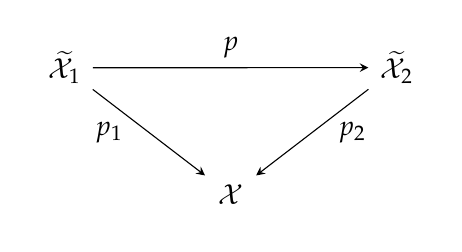
\begin{tikzpicture}
			\matrix (m) [matrix of math nodes,row sep=3em,column sep=4em,minimum width=2em]
			{
				\widetilde{\mathcal X}_1 & &\widetilde{\mathcal X}_2\\ 
				& {\mathcal X}\\};
			\path[-stealth]
			(m-1-1) edge node [above] {$p$} (m-1-3)
			(m-1-1) edge node [left]  {$p_1~~$} (m-2-2)
			(m-1-3) edge node [right] {$~~p_2$} (m-2-2);
		\end{tikzpicture}
		\\
		where $\sX$ is locally connected (cf. Definition \ref{top_locally_connected_defn}) and $p_1$, $p_2$ are covering projections. If $p$ is a surjection then $p$ is a covering projection.
	\end{corollary}
	\begin{theorem}\label{top_locally_conn_cov_com_thm}\cite{spanier:at}
		If   $p: \widetilde{\mathcal X}\to {\mathcal X}$ is a covering projection onto locally connected base space, then for any component  $\widetilde{\mathcal Y}$ of $\widetilde{\mathcal X}$ the map
		$$
		p|_{\widetilde{\mathcal Y}}:\widetilde{\mathcal Y} \to p\left(\widetilde{\mathcal Y} \right) 
		$$
		is a covering projection onto some component of $\widetilde{\mathcal X}$.
	\end{theorem}
	%\begin{lemma}\label{top_covp_cat_lem}  	\ref{top_finite_covering_thm}}
	%In the {category of connected covering spaces} of a connected locally path-connected space every morphism is itself a covering projection.
	%\end{lemma}
	\begin{theorem}\label{top_conjugate_thm}\cite{spanier:at}
		Let $p_1: 	\widetilde{\sX}_1 \to \sX$, $p_2: 	\widetilde{\sX}_2 \to \sX$ be objects  in the category of connected covering spaces of a connected locally path-connected space $\sX$. The following are equivalent
		\begin{enumerate}
			\item [(a)] There is a covering projection $f:\widetilde{\sX}_1 \to \widetilde{\sX}_2$ such that $p_2 \circ f = p_1$.
			\item[(b)] For all $\widetilde{x}_1\in \widetilde{\sX}_1$ and  $\widetilde{x}_2\in \widetilde{\sX}_2$ such that $p_1\left(\widetilde{x}_1 \right) = p_2\left(\widetilde{x}_2 \right)$, $\pi_1\left(p_1\right)\left( \pi_1 \left( \widetilde{\sX}_1, \widetilde{x}_1\right)  \right)$ is conjugate to a subgroup of  $\pi_1\left(p_2\right)\left( \pi_1 \left( \widetilde{\sX}_2, \widetilde{x}_2\right)  \right)$.
			\item[(c)] There exist $\widetilde{x}_1\in \widetilde{\sX}_1$ and  $\widetilde{x}_2\in \widetilde{\sX}_2$ such that $\pi_1\left(p_1\right)\left( \pi_1 \left( \widetilde{\sX}_1, \widetilde{x}_1\right)  \right)$ is conjugate to a subgroup of  $\pi_1\left(p_2\right)\left( \pi_1 \left( \widetilde{\sX}_2, \widetilde{x}_2\right)  \right)$.
		\end{enumerate} 
	\end{theorem}
\begin{definition}\label{local_homeomorphism_defn}\cite{spanier:at}
A continuous map $f: \sX \to \sY$ is called a \textit{local homeomorphism} if each 
point $y \in \sY$ has an open neighbourhood mapped homeomorphically by $f$ onto 
an open subset of $\sX$
\end{definition}
\begin{lemma}\label{top_cov_lem}\cite{spanier:at}
	A covering projection is a local homeomorphism.
\end{lemma}

	\begin{lemma}\label{top_om_lem}\cite{spanier:at}
		A local homeomorphism is an open map (cf. Definition \ref{top_onen_map_defn}).
	\end{lemma}
	
	
	\begin{remark}\label{top_cov_bicont_rem}
 From the Lemmas \ref{top_om_lem} and \ref{top_om_lem} it follows that any covering is a bicontinuous map (cf. Definition \ref{top_bicont_defn}).
	\end{remark}
	


	\begin{defn}\label{top_path_lifting_defn}\cite{spanier:at}
		A continuous map $p:\mathcal{E} \to \mathcal{B}$ is said to have the {\it unique path lifting} if, given paths $\omega$ and $\omega'$ in $E$ such that $p \circ \omega = p \circ \omega'$ and $\omega(0)=\omega'(0)$, then $\omega=\omega'$.
	\end{defn}
	\begin{thm}\cite{spanier:at}\label{spanier_thm_un}
		Let $p: \widetilde{\mathcal{X}} \to \mathcal{X}$ be a covering projection and let $f, g: \mathcal{Y} \to \widetilde{\mathcal{X}}$ be liftings of the same map (that is, $p \circ f = p \circ g$). If $\mathcal{Y}$ is connected and $f$ agrees with g for some point of $\mathcal{Y}$ then $f=g$.
	\end{thm}
	\begin{rem}
		From theorem \ref{spanier_thm_un} it follows that a covering projection has unique path lifting.
	\end{rem}
	
	\subsubsection{Regular and universal coverings}
	\begin{defn}\label{top_regular_defn}\cite{spanier:at}
		A fibration $p: \mathcal{\widetilde{X}} \to \mathcal{X}$ with unique path lifting is said to be  {\it regular} if, given any closed path $\omega$ in $\mathcal{X}$, either every lifting of $\omega$ is closed or none is closed.
	\end{defn}
	\begin{thm}\label{locally_path_thm}\cite{spanier:at}
		Let $p: \widetilde{\mathcal X} \to \mathcal X$ be a fibration with unique path lifting and assume that a nonempty $\widetilde{\mathcal X}$ is a locally path-connected space. Then $p$ is regular if and only if for some $\widetilde{x}_0 \in  \widetilde{\mathcal X}$, $\pi_1\left(p\right)\pi_1\left(\widetilde{\mathcal X}, \widetilde{x}_0\right)$ is a normal subgroup of $\pi_1\left(\mathcal X, p\left(\widetilde{x}_0\right)\right)$.
	\end{thm}
		\begin{definition}\label{top_properly_disc_group_defn}\cite{spanier:at} 
		A group $G$ of homeomorphisms of a topological space $\sY$  is said to be  
		\textit{discontinuous} if the orbits of $G$ in $\sY$ are discrete subsets of $\sY$. $G$ is \textit{properly discontinuous} if for $y \in \sY$ there is an open neighbourhood $\sU$ of $y$ in $\sY$ such 
		that if $g, g' \in  G$ and $g\sU$ meets $g'\sU$, then $g = g'$. $G$ \textit{acts without fixed points} if the only element of $g\in G$ having fixed points is the identity element.	
	\end{definition}
	\begin{remark}\label{top_properly_disc_rem}\cite{spanier:at}
		A finite group of homeomorphisms acting without fixed points on a 
		Hausdorff space is properly discontinuous.
	\end{remark}
	\begin{theorem}\label{top_group_of_covering_transformations_thm}\cite{spanier:at}
		Let $G$ a properly discontinuous group of homeomorphisms 
		of a space $\sY$. Then the projection of $\sY$ to the orbit space $\sY/G$ is a covering projection. If $\sY$ is connected, this covering projection is regular and $G$  is its	group of covering transformations. 
	\end{theorem}
\begin{lem}\label{top_cov_from_pi1_cor}\cite{spanier:at}
		Let $p: \widetilde{\mathcal X} \to \mathcal X$ be a fibration with a unique path lifting. If $ \widetilde{\mathcal X}$ is connected and locally path-connected and $\widetilde{x}_0 \in \widetilde{\mathcal X}$ then $p$ is regular if and only if $G\left(\widetilde{\mathcal X}~|~{\mathcal X} \right)$ principal  \ref{top_principal_defn} ly acts on each fiber of $p$, in which case 
		$$
		\psi: G\left(\widetilde{\mathcal X}~|~{\mathcal X} \right) \approx \pi_1\left(\mathcal X, p\left( \widetilde{x}_0\right)  \right) / \pi_1\left( p\right)\pi_1\left(\widetilde{\mathcal X}, \widetilde{x}_0 \right)  
		$$
		where $\pi_1$ denotes fundamental groups (cf. Remark \ref{top_homotopy_group_rem}).
	\end{lem}
	\begin{remark}\label{top_sim_con_reg_rem}\cite{spanier:at}
		If $\widetilde{   \sX}$ is simply connected, any fibration $p: \widetilde{   \sX} \to \sX$ is regular, and we also have the next result.
	\end{remark}
	\begin{cor}\label{top_cov_pi1_cor}\cite{spanier:at}
		Let $p: \widetilde{\mathcal X} \to \mathcal X$ be a fibration with a unique path lifting where $ \widetilde{\mathcal X}$ is simply connected locally path-connected and nonempty.  Then the group of self-equivalences of $p$ is isomorphic to the fundamental group of ${\mathcal X}$ (cf. Remark \ref{top_homotopy_group_rem}), i.e. $\pi_1\left( {\mathcal X}\right)\approx G\left(\left.\widetilde{\sX}~\right|\sX\right)$.  
	\end{cor}
	
	\begin{theorem}\label{top_gr_cov_thm}\cite{spanier:at}
		%13 theorem
		Let $\sX$ be a connected locally path-connected space and let 
		$x_0\in \sX$. Let $H$ be a subgroup of $\pi_1\left( \sX, x_0\right)$  and assume  there is an open  
		covering $\mathscr U$ of $\sX$ such that $\pi_1\left(\mathscr U, x_0 \right)\subset H$ . Then there is a covering projection $p:\left(  \widetilde \sX, \widetilde x_0\right) \to \left(\sX, x_0 \right)$ such that  $p_{\#}\left(\widetilde \sX, \widetilde x_0 \right)= H$ . 
	\end{theorem}
	
	\begin{definition}\label{top_universal_covering_defn}\cite{spanier:at}
		A \textit{universal covering space} of a connected space $\sX$ is an object $p: \widetilde{\sX}\to \sX$ of the category of connected covering spaces of $\sX$ such that for any object $p': \widetilde{\sX}'\to \sX$ of this category there is a morphism 
		\newline
		\begin{tikzpicture}
			\matrix (m) [matrix of math nodes,row sep=3em,column sep=4em,minimum width=2em]
			{
				\widetilde{\sX}  &  & \widetilde{\sX}'\\
				& \sX & \\};
			\path[-stealth]
			(m-1-1) edge node [above] {$f$} (m-1-3)
			(m-1-1) edge node [left]  {$p~~$} (m-2-2)
			(m-1-3) edge node [right] {$~~p'$} (m-2-2);
			%\draw[dashed,->]   (m-1-1) -- (m-1-3);
		\end{tikzpicture}
		\\
		in the category.
	\end{definition}
	
	\begin{lem}\label{top_simply_con_cov_lem}\cite{spanier:at}
		A connected locally path-connected space $\mathcal X$ has a simply connected covering space $\widetilde{\sX}$ if and only if  $\mathcal X$ is semilocally 1-connected (cf. Definition \ref{top_semi1_defn}).
	\end{lem}
\begin{remark}\label{top_simply_con_cov_rem}
Under the hypothesis of the Lemma \ref{top_simply_con_cov_lem} there is an isomorphism
$$
\pi_1\left(\sX, x_0 \right)\cong G\left(\left.\widetilde \sX \right| \sX\right).  
$$
\end{remark}	
	%\begin{lem}\label{top_simply_con_uni_cor}\cite{spanier:at}
	%	Any universal covering space of a connected locally path connected semilocally 1-connected space is simply connected.
	% \end{lem}
	%\begin{lem}\label{top_uni_spa_lem}\cite{spanier:at}
	% 	Two universal covering spaces of a connected locally path-connected space are equivalent.
	% \end{lem}
	
	\begin{lem}\label{top_uni_exist_spa_lem}\cite{spanier:at}
		A simply connected covering space of a connected locally path-connected space $\sX$ is an universal covering space of $\sX$.
	\end{lem}
	
	




\begin{prop}\cite{switzer:at} \label{top_pi1_pi1_prop}
	(cf. Proposition 3.30).
	If $\sX$ is a topological space then there is an action of $\pi_1\left(\sX\right)\times \pi_1\left(\sX\right)\to \pi_1\left(\sX\right)$ given conjugation; i.e. such that for $\ga, \a \in \pi_1\left(\sX\right)$ one has $\ga \cdot \a = \ga \a\ga^{-1}$.
\end{prop}


\subsection{Homology theory and Hurewicz homomorphism}

\begin{definition}\label{top_unred_defn}\cite{switzer:at}
	Let $\mathscr T^2$ denote the category of all topological pairs $\left(\sX, \A\right)$ ($\A\subset\sX$ a subspace) and maps $f: \left(\sX, \A\right)\to \left(\sY, \B\right)$. On $\mathscr T^2$  we have the functor $R:\mathscr T^2$ ("restriction") defined by $R\left(\sX, \A\right)= \left(\A, \emptyset\right)$, $R\left(f \right)= f|_{\A}$. Let $\mathscr T^2~'$ be the homotopy category - i.e. objects are as in $\mathscr T^2$, morphisms are homotopy classes of maps. We still  have $R:\mathscr T^2~'\to \mathscr T^2~':$ $R\left(\sX, \A\right)= \left(\A, \emptyset\right)$, $R\left(\left[f\right] \right)= \left[f|_{\A}\right]$. 
	
	An \textit{unreduced homology theory} $h_*$ on $\mathscr T^2~'$ is a sequence of functors $h_n$ from $\mathscr T^2~'$ to the category of Abelian groups  for each $n\in \Z$ and the natural transformations $\partial_n : h_n \to h_{n-1}\circ R$, satisfying the following two axioms:
	\begin{enumerate}
		\item [(a)] Exactness: for every pair $\left(\sX, \A\right)\in\mathscr T^2~'$ the sequence
		\bean
		...\to h_{n+1}\left(\sX, \A\right)\xrightarrow{\partial_{n+1}\left(\sX, \A\right)} h_{n}\left(\A, \emptyset\right)\xrightarrow{hurewicz_n\left[i\right]}h_{n}\left(\sX, \emptyset\right)\xrightarrow{hurewicz_n\left[j\right]}\\
		h_{n}\left(\sX, \A\right)\xrightarrow{\partial_{n}\left(\sX, \A\right)}
		\eean
		is exact where $i: \left(\A, \emptyset\right)\to \left(\sX, \emptyset\right)$ and $j: \left(\sX, \A\right)\to \left(\sX, \emptyset\right)$ are the inclusions.
		\item[(b)] Excision: for every pair $\left(\sX, \A\right)$ and open subset $\sU\in \A$ with $\overline{   \mathcal U }\subset \mathring{\A}$ the inclusion $j: \left(\sX\setminus \sU, \A\setminus \sU\right)\to \left(\sX, \A\right)$ induces an isomorphism $h_n\left[j\right]: h_n\left(\sX\setminus \sU, \A\setminus \sU\right)\to h_n\left(\sX, \A\right)$.
	\end{enumerate}
	\end{definition}
	\paragraph{}
Let $\mathscr {PT}$ be a category of  pointed spaces and let $\mathscr {PT}'$ be a homotopy category, i.e. objects are as in $\mathscr {PT}$, morphisms are homotopy classes of maps.
\begin{definition}\label{top_suspension_defn}\cite{switzer:at}
On $\mathscr {PT}'$ we have a \textit{suspension functor} $S\left(\sX, x_0 \right)\bydef\left( S\sX, *\right)$ and $S\left[f \right]\bydef\left[Sf \right]   \bydef \left[1_{S^1} \wedge f\right]$ 
\end{definition}

 
\begin{definition}\label{top_red_homol_defn}
A \textit{reduced homology theory} $k_*$ on $\mathscr {PT}'$ is a collection of functors $k_n: \mathscr {PT}'\to \mathscr A$ to the category of Abelian groups and natural equivalences $\sigma_n: k_n \to k_{n+1}\circ S$, satisfying
	\begin{enumerate}
			\item [(a)] \textit{Exactness}: for every  pointed pair $\left(\sX, \A, x_0\right)$ with inclusions $\iota:\left( \sX, x_0\right) \to \left( \sX_0\right)$ and $j : \left( \sX\cup C\A, *\right)$ the sequence 
		\bean
	k_n\left(\A, x_0\right)\xrightarrow{k_n\left[\iota\right]} k_n\left( \sX, x_0\right)\xrightarrow{k_n\left[j\right]} \left( \sX\cup C\A, *\right)	
	\eean
		is exact.
	\end{enumerate}

\end{definition}

\begin{proposition}
There are natural transformations $\hat \partial_n $ and for each  pointed pair $\left(\sX, \A, x_0\right)$ a long exact sequence
		\bean
	k_n\left(\A, x_0\right)\xrightarrow{k_n\left[\iota\right]} k_n\left( \sX, x_0\right)\xrightarrow{k_n\left[j\right]} \left( \sX\cup C\A, *\right)	
\xrightarrow{\hat \partial_n\left(\sX, \A, x_0\right)}\\	\xrightarrow{\hat \partial_n\left(\sX, \A, x_0\right)}	k_{n-1}\left(\A, x_0\right)\xrightarrow{k_{n-1}\left[\iota\right]}...
\eean
\end{proposition}  
\begin{definition}\label{top_hurewitz_defn}\cite{switzer:at}
	% 7.39
	Let $k_*$ be a reduced homology theory. We define the \textit{Hurewicz homomorphism} 	$h:\pi_n\left(\sY, y_0 \right)\to k_n\left(\sY \right)$  to be the composite
	\be
	\begin{split}
		\pi_n\left(\sY, y_0 \right)\cong \left[S^n, s_0; \sY, y_0\right]\xrightarrow{k_n}\Hom\left(k_n\left(S^n \right),  k_n\left(\sY \right)\right) \xrightarrow{\Hom\left(\sigma^n, 1 \right) }\\
		\Hom\left(k_n\left(S^0 \right),  k_n\left(\sY \right)\right)\cong k_n\left(\sY \right).
	\end{split}
	\ee
\end{definition}

Any homology theory defines a cohomology theory. In particular it satisfies to the following exactness axiom
\be\label{top_c_exact_eqn}
...\xrightarrow{\delta} k^n\left(\sX, \A \right) \xrightarrow{k^n\left[j\right]} k^n\left(\sX \right) \xrightarrow{k^n\left[i\right]} k^n\left(\A \right) \xrightarrow{\delta} k^{n+1}\left(\sX, \A \right)\to ...
\ee
\begin{theorem}\cite{rotman:ag}
%Theorem 4.29 (Hurewicz 7 Theorem).
 If $\sX$ is path connected, then the Hurewicz
map $\varphi: \pi_1\left(\sX, x_0 \right) \to H_1\left( \sX\right)$  is a surjection with kernel $\pi_1\left(\sX, x_0 \right)'$, the commutator
subgroup of $\pi_1\left(\sX, x_0 \right)$. Hence
$$
\pi_1\left(\sX, x_0 \right)/\pi_1\left(\sX, x_0 \right)'\cong H_1\left( \sX\right).
$$
\end{theorem}
We shall use the following equivalent formulation of the above theorem.
\begin{theorem}\label{hurewicz_iso_thm}
	If $H_*$ is the theory of singular homology then the following Hurewicz homomorphism
	$$
	h_{\mathrm{sing}}:\pi_1\left( \sX\right) / \left[\pi_1\left( \sX\right), \pi_1\left( \sX\right)\right]\to H_1\left(\sX \right) 
	$$
	is an isomorphism.
\end{theorem}
\begin{theorem}\label{top_h_to_k_thm}\cite{switzer:at}
For every topological pair $\left(\sX, \A\right)$ and Abelian group $G$ there is a natural exact sequence
\bean
0 \to \mathrm{\Ext}\left(H_{n-1}\left(\sX, \A\right),G \right)\to H^{n}\left(\sX, \A;G \right)\xrightarrow{\mu^*}\\\mathrm{Hom}\left(H_{n}\left(\sX, \A \right), G\right) \to 0
\eean
and unnatural splitting
$$
H^{n}\left(\sX, \A;G \right)\cong \mathrm{\Ext}\left(H_{n-1}\left(\sX, \A \right),G \right)\oplus\mathrm{Hom}\left(H_{n}\left(\sX, \A\right) ,G \right).
$$
\end{theorem}


%\subsection{Obstruction theory}
%\begin{definition}\label{top_char_defn}\cite{spanier:at}
%	Let $\pi$ an Abelian group and $\sY$ is a path-connected  pointed space. An element $v \in H^n\left(\sY, y, \pi \right)$ is said to be $n$-\textit{characteristic} for $\sY$ if the composite
%	$$
%	\pi_n\left(\sY, y_0 \right)\xrightarrow{\varphi} H^n\left(\sY, y, \pi \right)\xrightarrow{h(v)}\pi
%	$$ 
%	is isomorphism (where $\varphi$ is the Hurewicz homomorphism and $h\left( v\right)$ is the natural homomorhism which follows from the universal coefficient theorem  \cite{spanier:at}).
%\end{definition}
%\begin{definition}\label{top_pi_n_defn}\cite{spanier:at}
%Let $\pi$ be a group and let $n$ be an integer $\ge 1$. A space of type $\left(\pi, n\right)$ is a path-connected  pointed space $\sY$ such that $\pi_q\left(\sY \right)= 0$  for $q\neq n$ and 
$\pi_n\left(\sY \right)= 0$ is isomorphic to $\pi$.
%\end{definition}
%\begin{theorem}\label{top_obstr_thm}\cite{spanier:at}
	%12 theorem 
%	Let $\sY$ be a space of type $\left(\pi, n\right)$, with $n\ge 1$ and $\pi$ Abelian, and let $\iota$ be $n$-characteristic for $\sY$. If $(\sX,\A)$ is a relative $CW$-complex, a map $f: \A\to \sY$ 
%	can be extended over   $\sX$ if and only if $\delta H^n\left[f\right]\left( \iota \right)  = 0 \in  H^{n + 1}\left(\sX, \sA; \pi \right)$. 
%\end{theorem}
%\begin{remark}\label{top_obstr_rem}
%A notion of  a (relative) $CW$-complex is explained in \cite{spanier:at,switzer:at}.
%\end{remark}
%\begin{remark}
%	The  Theorem \ref{top_obstr_thm} implies the cohomology exact sequence %\eqref{top_c_exact_eqn}, i.e.
%	\bean
%	...\xrightarrow{\delta} H^n\left(\sX, \A ;\pi\right) \xrightarrow{H^n\left[j\right]} H^n\left(\sX ;\pi\right) \xrightarrow{H^n\left[i\right]} H^n\left(\A; \pi \right) \xrightarrow{\delta} H^{n+1}\left(\sX, \A ;\pi\right)\to ...
%	\eean
%	and a homomorphism $H^n\left[f\right]: H^n\left(\sY; \pi \right) \to H^n\left(\A; \pi \right)$.
%\end{remark}
	\section{Vector bundles and elements of $K$-theory}\label{top_vb_sub_sub}
	\subsection{Vector bundles}
\paragraph*{}
Let $k$ be the field of real or complex numbers, and let $\sX$ be a topological space.
\begin{definition}\label{top_vb_fiber_defn}\cite{karoubi:k}
	A \textit{quasi-vector bundle with base} $\mathcal X$ is given by:
	\begin{enumerate}
		\item [(a)] A finite dimensional $k$-vector space $E_x$ for every point $x$ of $\mathcal X$.
		\item[(b)] A topology on the disjoint union $E = \bigsqcup E_x$ which induces the natural topology on each $E_x$, such that the obvious projection $\pi: E \to  \mathcal X$ is continuous.
	\end{enumerate}
	The quasi-vector bundle with base will be denoted by $\xi = \left( E, \pi, \mathcal X\right)$. The space $E$ is the \textit{total space} of $\xi$ and $E_x$ is the \textit{fiber} of $\xi$ at the point $x$.
\end{definition}
\begin{empt}\label{trivial_vb_empt}\cite{karoubi:k}	Let $V$ be a finite dimensional vector space over $k$,  $E_x = V$ and the total space may be identified with $\sX \times V$ with the product topology then the quasi-vector bundle  $\left(\sX \times V, \pi, \mathcal X\right)$ is called a \textit{trivial vector bundle}.
\end{empt}
\begin{empt}\cite{karoubi:k}	Let $\xi = \left( E, \pi, \mathcal X\right)$ be a quasi-vector bundle, and let let $\sX' \subset \sX$ be a subspace of $\sX$. The triple $\xi' = \left(\pi^{-1}\left( \sX'\right) , \pi|_{\pi^{-1}\left( \sX'\right)}, \mathcal X'\right)$ is called the \textit{restriction} of $\xi$ to $\sX'$. The fibers of $\xi'$ are just fibers of $\xi$ over the subspace $\xi$. One has
	\be
	\sX'' \subset \sX' \subset \sX \quad \Rightarrow\quad \left.\left(\xi|_{\sX'} \right) \right|_{\sX''}= \xi|_{\sX''}.
	\ee
\end{empt}
\begin{definition}\label{top_vb_defn}\cite{karoubi:k}
	Let $\xi = \left( E, \pi, \mathcal X\right)$ be quasi-vector bundle. Then $\xi$ is said to be \textit{locally trivial} or a \textit{vector bundle} if for every point $x$ in $\sX$, there exists a neighbourhood of $x$ such that $\xi|_{\sU}$ is isomorphic to a trivial bundle.
\end{definition}
\begin{definition}\label{top_vb_cs_defn}\cite{karoubi:k}	
	%	5.1. Definition.
	Let $\xi \bydef \left( E, \pi, \mathcal X\right)$ be a vector bundle. Then a \textit{section} of $\xi$ is a map $s: \sX \to E$ such that $\pi \times s = \Id_{\sX}$. A section $s$ is called \textit{continuous} if $s$ is a continuous. The space $\Ga\left({\mathcal X}, {E}\right)$, of continuous sections can be regarded as both left  and right $C_b\left(\mathcal{X} \right)$-module.
\end{definition}
\begin{notation}\label{top_sec_notn}
	We denote by $\Ga\left( M, E\right)$ the $\C$-space of continuous sections. Both  $\Ga_0\left( M, E\right)$ and $\Ga_c\left( M, E\right)$ are subspaces of  sections tending to zero at infinity and having compact support.
\end{notation}
\begin{remark}
	In \cite{karoubi:k} the vector bundles! with base  fields $\R$ and $\C$ are considered. Here we consider complex vector bundles only.
\end{remark}
% 	We refer to \cite{karoubi:k} for a notion of {\it (locally trivial) vector bundle}. 	Any {\it (locally trivial) vector bundle} with base $\mathcal X$ is a special case of \textit{quasi-vector bundle} which is a triple $\left(E, \pi, \mathcal X \right)$. 
\begin{definition}\label{vb_inv_img_funct_defn}\cite{karoubi:k}
	Let $f: \mathcal X' \to \mathcal X$ be a continuous map. For every point $x'$ of $\mathcal X'$, let $E'_{x'}= E_{f\left(x' \right) }$. Then the set $E' = \bigsqcup_{x' \in \mathcal X'}E'_{x'}$ may be identified with the \textit{fiber product} $\mathcal X' \times_{\mathcal X} E$ formed by the pairs $\left(x',e \right)$ such that $f\left(x' \right) = \pi\left( e\right)$. If  $\pi': E' \to \mathcal X'$ is defined by $\pi'\left(x',e \right) = x'$, it is clear that the triple $\xi = \left( E', \pi', \mathcal X'\right)$ defines a quasi-vector bundle  with base  $ \mathcal X'$, when we provide $E'$ with the topology induced by $ \mathcal X' \times E$. We write $\xi' = f^*\left(\xi \right)$ or $f^*\left(E \right)$: this is the \textit{inverse image} of $\xi$ by $f$.  
\end{definition}
\begin{theorem}\label{serre_swan_thm}\cite{karoubi:k}.
	Theorem (Serre, Swan). Let $A = C_k(\sX)$ be the ring of continuous 
	functions on a compact space $\sX$ with values in $k$. Then the section functor $\Ga$ (cf. Notation \ref{top_sec_notn}) induces an 
	equivalence of categories of vector bundles  with base  $\sX$ and finitely generated projective $A$-modules.
\end{theorem}

\begin{definition}\label{top_herm_bundle_form_defn}\cite{karoubi:k}
	%8.1. Definition. 
	Let $E$ be a vector bundle over $\C$. A \textit{sesquilinear form} on $E$ is a 
	continuous map $\varphi: E \times_\sX E \to \C$ which has the following property. The map 
	$\varphi_x : E_x \times E_x$ induced on each fiber is "sesquilinear" with respect to the $\C$-vector space structure of $E_x$. In other words, ($\varphi_x$ is $\R$-bilinear and $\varphi_x\left(\la e, e' \right)  = \varphi_x\left( e, \overline \la e' \right) = \la \varphi_x\left( e, e' \right)$ f
	for $\la\in \C$, $e \in E_x$, and $e' \in E_x$. 
\end{definition}





%Following fact is an implication of definitions.
%\begin{fact}\label{inv_image_fact}
%	A map $\varphi^*$ is an inverse image of $\varphi$ if and only if the above diagram is commutative for any $\mathcal U$ such that $\pi |_{\mathcal U}: \mathcal U \to \pi ({\mathcal U})$ is a homeomorphism.
%\end{fact}

\begin{remark}\label{top_herm_bundle_rem}
	Let $\mathcal X$ be a locally compact topological space and $E$ the complex vector bundle on $\mathcal X$ with a {sesquilinear form} $\varphi: E \times_\sX E \to \C$ then there are the following pairings
	\bea\label{top_gg_eqn}
	\left\langle \cdot, \cdot \right\rangle:  \Ga_0\left( \sX, E\right)\times \Ga_0\left( \sX, E\right) \to C_0\left( \sX\right) \quad \left(\xi, \eta \right) \mapsto \left(x \mapsto \varphi_x\left(\xi_x, \eta_x \right)  \right) ,\\
	\label{top_ggc_eqn}
	\left\langle \cdot, \cdot \right\rangle_c:  \Ga_c\left( \sX, E\right)\times \Ga_c\left( \sX, E\right) \to C_c\left( \sX\right) \quad \left(\xi, \eta \right) \mapsto \left(x \mapsto \varphi_x\left(\xi_x, \eta_x \right)  \right) 
	\eea
	(cf. Notation \ref{top_sec_notn}).
\end{remark}




\subsection{The Fundamental Product Theorem}\label{k_fund_prod_sec}

\paragraph{}
 We assume knowledge of elementary notions of $K$-theory explained in \cite{atiyah:kt,hatcher:kt,karoubi:k}.
The key result allowing the calculation of $K\left( \sX\right)$  in nontrivial cases is a certain formula
that computes $K\left(\sX \times S^2 \right)$  in terms of  $K\left(\sX \times S^2 \right)$. For example, when $\sX$ is a point this
will yield a calculation of $K\left(S^2 \right)$.  Any point of the projective space $\C P^1$ yields a one-dimensional $\C$-subspace  of $\C^2$. So there is a $\C$-bundle over $\C P^1$ which sets to any point of $\C P^1$ the corresponding subspace. Using a homeomorphism $S^2 \cong \C P^1$ we define 
be the canonical line bundle $H$ with base   $S^2 \cong \C P^1$, and let $1$ is a trivial bundle then according to  in \cite{atiyah:kt}  one has
\bean
\left(H \otimes H \right) \oplus 1 \cong H \oplus H,\\
H^2 +1 = 2H.
\eean
We can also write this as $\left( H - 1\right)^ 2$ = 0, so we have a natural ring homomorphism
$\Z\left[H\right]/\left( H - 1\right)^2\cong  K\left( S^2\right)$  whose domain is the quotient ring of the polynomial ring
$\Z\left[H\right]$ by the ideal generated by $\left( H - 1\right)^2$ . In particular, note that an additive basis for
$\Z\left[H\right]/\left( H - 1\right)^2$ is $\left\{1, H\right\}$.
\subsection{Fredholm picture of $K$-theory}
\paragraph{} % PAGE 108
Here I follow to \cite{karoubi:k}.  Let $\mathscr H$ be the category of Hilbert spaces and let $\check{\mathscr H}$ be the category with the 
same objects but with $\check{\mathscr H}\left(E, F \right)  = {\mathscr H}\left(E, F \right)/\K(E, F)$, where $\K(E, F)$ denotes the 
set of completely continuous operators from $E$ to $F$ (i.e. the operators which are 
limits of operators of finite rank). 
\begin{exercise}
	a) Prove that a morphism $D: E \to F$ in the category ${\mathscr H}$ is invertible in $\check{\mathscr H}$ if and 
	only if $D$ is a Fredholm operator (i.e. $\ker D$ and $\coker D$ are finite dimensional).\\ 
	b) Let $d: E \to F$ be an invertible morphism of $\check{\mathscr H}$, and let $D$ be an operator in ${\mathscr H}$ 
	with class $d$. Prove that the "\textit{index}" of $D$ (i.e. $\dim\ker D - \dim\coker D$) is 
	independent of the choice of $D$, and is a locally constant function of $d$. \\
	c) Prove the isomorphism $K^{-1} \left( \check{\mathscr H}\right) \cong \Z$.
\end{exercise}
\begin{exercise}\label{ex_karouby_exer} %PAGE 176
 Let $\H$ be a Hilbert space of infinite dimension over  $k=\R$ or $\C$, and let 
$GL_c\left( \H\right)$  be the subgroup of $GL\left( \H\right)$  consisting of operators of the form $1+ u$, 
where $u$ is compact
\begin{enumerate}
	\item [(i)]  If $\sX$ is a compact space, prove that $\left[\sX, GL_c\left( \H\right) \right] \cong K^{-1}\left(\sX \right) \cong \left[\sX, GL\left(k \right) \right]$.
\item[(ii)] Let $\mathscr F\left(\H \right)$  be the set of Fredholm operators $D$ in $\H$ (i.e. such that $\ker D$ 	and $\coker D$ are finite dimensional). Using the fact that $GL\left( \H\right)$  is connected 
	 prove that the map $D \mapsto \dim \ker D - \dim \coker D$ (= \textit{index} of $D$) 	induces a bijection $\pi_0 \left(\mathscr F\left(\H \right) \right) \cong \Z$
	\item[(iii)] Let $\mathscr F\left(\H \right)^0$ be the subset of $\mathscr F\left(\H \right)$ consisting of operators of index $0$. 
	Prove the fibration 
	$$
\mathscr F\left(\H \right)^0
	$$ 
\end{enumerate}
Using the fact that $GL\left(\H \right) $ is contractible  prove that $\Om \mathscr F\left(\H \right)^0\cong GL_c\left(\H \right)$, and that $K\left( \sX\right) \cong \left[\sX, \mathscr F\left(\H \right)\right]$.		
\end{exercise}
\subsection{The group $K\left(\sX, \sY \right)$}
\begin{theorem}\label{k_ext_thm}\cite{karoubi:k}
%	5.10. Theorem. 
Let $\E$ and $\F$ be vector bundles with base  a paracompact space $\sX$, let $\sY$ be 
	a closed subset of $\sX$, and let  $\a: \E_\sY \to \F_\sY$ be a morphism of vector bundles. Then there 
	exists a morphism $\widetilde \a: \E \to \F$such that $\widetilde \a|_\sY= \a$ ($\widetilde \a$ is called an "extension" of $\a$ to $\sX$). 
\end{theorem}
\begin{corollary}\label{k_ext_cor}\cite{karoubi:k}
%5.11. Corollary. 
With the notation of Theorem \ref{k_ext_cor}, let us suppose that a is an 
isomorphism. Then there exists a neighbourhood $\sV$ of $\sY$ and an isomorphism 
$\a': \E_\sV \to \F_\sV$ such that $\a'_\sY = \a$. 
\end{corollary}
\begin{definition}\cite{karoubi:k}
%2.1. Definition. 
Let $\mathscr C$ be an additive category. A \textit{Banach structure} on $\mathscr C$ is given by 
a Banach space structure on all the groups $\mathscr C\left(\E, \F \right) $, where $\E$ and $\F$ run through the objects of $\mathscr C$. Moreover , we assume that the map 
$$
\mathscr C\left(\E, \F \right)\times \mathscr C\left(\F, \G \right)\to \mathscr C\left(\E, \G \right)
$$
given by the composition of morphisms, is bilinear and continuous (all Banach 
spaces are over  the basic field $k=\R$  or $\C$). A \textit{Banach category} is an additive category provided with a Banach structure. 

\end{definition}
\begin{definition}\cite{karoubi:k}
%2.6. Definitions. 
Let $\mathscr C$ and $\mathscr C'$ be additive categories, and $\varphi: \mathscr C\to\mathscr C'$ be an additive.
functor. Then $\varphi$ is called \textit{quasi-surjective} if every object of $\mathscr C'$ is a direct factor of an 
object of the form $\varphi\left(\E \right) $, where $\E\in \mathrm{Ob}\left(\mathscr C \right)$ ; $\varphi$ is called \textit{full} if the map $\mathscr C\left(\E, \F \right)\to \mathscr C\left(\varphi\left( \E\right) , \varphi\left( \F\right)  \right)$ is surjective for $\E, \F\in \mathrm{Ob}\left(\mathscr C \right)$, Finally, if $\mathscr C$ and $\mathscr C'$ are Banach 
		categories, the functor $\varphi$ is called a \textit{Banach functor} if the $\mathscr C\left(\E, \F \right)\to \mathscr C\left(\varphi\left( \E\right) , \varphi\left( \F\right)  \right)$ is linear and continuous. 
\end{definition}
\begin{empt}\label{k_triple_empt}\cite{karoubi:k}
%2.13.
 Let  $\varphi: \mathscr C\to\mathscr C'$ be a quasi-surjective Banach functor. We wish to define a "relative" group $K\left( \varphi\right)$  (which coincides with $K\left(\mathscr C \right)$ when $\mathscr C'=0$). Let $\Ga\left( \varphi\right)$ denote the set of triples $\left(\E, \F, \a \right)$, where $\E$ and $\F$ are objects of $\mathscr C$ and $\a : \varphi\left(\E \right)\to \varphi\left(\F \right)$  is an 
isomorphism. Two triples  $\left(\E, \F, \a \right)$ and  $\left(\E', \F', \a' \right)$ are called \textit{isomorphic} if there 
exist isomorphisms $f : \E \to \E'$ and $g : \F \to \F'$ such that the following diagram commutes. 
\newline
\begin{tikzcd}
\varphi\left( \E\right)\arrow[r, "\a"] \arrow[d, "\varphi\left( f\right) "]& \varphi\left( \F\right) \arrow[d, "\varphi\left( g\right) "]\\
\varphi\left( \E'\right)\arrow[r, "\a'"] & \varphi\left( \F'\right)
\end{tikzcd}

	A triple $\left(\E, \F, \a \right)$, is called \textit{elementary} if $\E=\F$ and if $\a$ is homotopic to $\Id_{\varphi\left(\E \right) }$ within 
	the automorphisms of $\varphi\left(\E \right)$. Finally, we define the sum of two triples $\left(\E, \F, \a \right)$ and $\left(\E', \F', \a' \right)$ to be $\left(\E\oplus \E', \F \oplus \F', \a \oplus \a'\right)$.
	Then $K\left( \varphi\right) $ is the quotient of $\Ga\left( \varphi\right) $ by the following equivalence relation: 
	$\sigma\sim \sigma'\Leftrightarrow\exists$ elementary $\tau$ and $\tau'$ such that $\sigma + \tau$ is isomorphic to $\sigma' + \tau'$ . The sum of 
	triples obviously provides the set $K\left(\varphi \right) $ with a monoid structure. We let $d\left(\E, \F, \a \right)$
	denote the class of $\left(\E, \F, \a \right)$ in the monoid $K\left(\varphi \right)$. %As a direct consequence of the 	definition, we notice that d(E, F, a) = 0 if and only if there exist objects G and 	H of #, and isomorphisms w: F � G�>H and v: F� G-> H9 such that 	<p(i>) � (a � Id^C)) � <p(w_!) is homotopic to Id^(H) within the automorphisms of(p(H). 

\end{empt}
\begin{example}\label{k_triple_exm}\cite{karoubi:k}
	%2.7. Example. 
	Let $\varphi: \mathscr E\left( \sX\right) \to  \mathscr\E\left(\sY \right)$  be the functor defined by $\varphi\left( \E\right) = \E|_\sY$ , where 
	$\sY$ is a closed subspace of the compact space $\sX$. It is proven in \cite{karoubi:k} that $\varphi$ 
	is a Banach functor which is full and quasi-surjective. We use the following notation
	$$
	K\left(\sX, \sY \right) \bydef K\left(\varphi \right) 
	$$
	%  By 1.5.9 we see that up to isomorphism the "restriction map" &(X){E, F)-> (Y)(EY, FY) is identical with the map r(X, HOM( , /0)-> 	r(Y, HOM(is, F)Y}. From 1.6.23, it follows that (p is a Banach functor. Moreover , (p is full A.5.10), and also quasi-surjective because any object of $( Y) is a directfactor of a trivial bundle 9n= Yxk" A.6.5), and clearly 6n = (p(E) where E=Xxk". 
\end{example}
\begin{example}\label{k_b_s_exm}\cite{karoubi:k}
	%2.30. Example. 
	Let $\sX \bydef B^2$ (resp. $\sY \bydef S^1$) be the unit ball(resp. sphere) in $\R^2$.Then 
	we define an element $d\left(\E, \F, \a \right)$ of $K\left(\sX, \sY \right)  = K\left(B^2, S^1 \right)$ by $\E= \F = B^2\times \C$ and $\a\left(x, v\right) =\left(x, xv\right)$. It is proven that $K\left(B^2, S^1 \right)$ is a generated by $d\left(\E, \F, \a \right)$ free Abelian group, i.e. $K\left(B^2, S^1 \right)=\Z~ d\left(\E, \F, \a \right)$.
	
\end{example}

\begin{proposition}\label{k_comp_prop}\cite{karoubi:k}
%2.16. Proposition.
 Let $d\left(\E, \F, \a \right)$ and $d\left(\F, \G, \bt \right)$ be elements of $K\left(\varphi \right)$. Then we have 
the relation
$$
d\left(\E, \F, \a \right) + d\left(\F, \G, \bt \right)= d\left(\E, \G, \bt\a \right)
$$ 

\end{proposition}
\begin{proposition}\label{k_exact_prop}\cite{karoubi:k}
%2.20. Proposition.
 Let $j: K\left(\varphi \right)\to K\left(\mathscr C\right)$  (resp. $k: K\left( \mathscr C \right)\to K\left( \mathscr C' \right)$  be the homomorphism 
	defined by $j\left( d\left(\E, \F, \a \right)\right) \bydef \left[\E\right]- \left[\F\right]$ (resp. $j\left( \left[\E\right]- \left[\F\right]\right) \bydef \left[\varphi\left( \E\right) \right]- \left[\varphi\left( \E\right)\right]$. Then we have an exact sequence 
	$$
K\left(\varphi\right)\xrightarrow{j} K\left(\mathscr C\right)\xrightarrow{k} K\left(\mathscr C'\right).
	$$ 
%	Moreover , if there exists a functor ij/'.W�tW such that (p\j/ � Id^,, f/ze� we have the 	split exact sequence 	0 > K((p) -U K(<#) -^-+ K(W) �^ 0. 
\end{proposition}
\begin{remark}\label{k_exact_rem}\cite{karoubi:k}
	If $\sY$ is a closed subspace of the compact space then from the Proposition \ref{k_exact_prop} it follows that there is the exact sequence
	$$
	K\left( \sX,\sY\right)\to K\left( \sX\right) \to K\left(\sY \right).
	$$
\end{remark}
\begin{theorem}\label{k_excision_thm}(Excision)\cite{karoubi:k}
%2.35. Theorem (Excision). 
The projection $\pi: \sX \to \sX/\sY$ induces an isomorphism 
$$
\pi^*:K\left( \sX/\sY,\{{y}\}\right) \xrightarrow{\cong }K\left( \sX,\sY\right).
$$
\end{theorem}
\begin{proof}
For $\sY$ empty, we leave the trivial verification to the reader. For $\sY$ 
nonempty, the proof breaks into two parts: \\
a) \textit{$\pi^*$ is surjective}. Let $ d\left(\E, \F, \a \right)$ be an element of $K\left( \sX,\sY\right)$. By adding the same 
bundle to $\E$ and $\F$, we may assume without loss of generality, that $\F$ is a trivial 
bundle, say $\mathcal{T}$. We want to find a triple $\left(\E', \F', \a \right)$ defining an element of 
$K\left( \sX/\sY,\{y\}\right)$ such that the triples $\left( \pi^*\left(\E'\right) , \pi^*\left(\F'\right) , \pi^*_1\left(\a\right)  \right)$ and $\left(\E, \F, \a \right)$ are  
isomorphic with $\pi_1: \sY \to \{y\}$. % According to 1.5.11, 
According to the Corollary \ref{k_ext_cor} there is a closed neighbourhood $\sV$ 
of $\sY$ and an isomorphism $\bt :\E_\sV\to  \F_\sV$ such that $\bt|_\sY = \a$. Let $\E'$ be the vector bundle 
 with base  $\sX/\sY$ obtained by clutching the bundle $\sE|_{\sX\setminus\sY}$ and the trivial bundle of rank $n$ 
 with base  $\sV \setminus\sY$, using $\bt|_{\sV \setminus\sY}$ (note that $\sX \setminus \sY \cong \sX/\sY \setminus \{y\}$ and $\sV \setminus \sY \cong \sV/\sY \setminus \{y\}$. Let $\sF'$ 
be the trivial bundle of rank $n$  with base  $\sX/\sY$, and let $\a': \E'|_{\{y\}} \to \F'|_{\{y\}}$ be the isomorphism 
induced by the above clutching. 

Then we can define an isomorphism $f: \E \to \pi^*\left( \E'\right)$  by $f_{\sX \setminus\sY}= \Id$, with the 
identification $\pi^*\left( \E'\right)|_{\sX\setminus \sY}=\E'|_{\sX\setminus \sY}=\E|_{\sX\setminus \sY}$, and $f|_\sV=\Id$ with the identification 
$\E'|_{\sV}= p_n|_{\sX\setminus \sY}$. It is now straightforward to check that the diagram 
\newline
\begin{tikzcd}
\E|_{\sY} \arrow[r, "\a"] \arrow[d, "f|_\sY"]& \F|_{\sY}\arrow[d, "\cong"]\\
\pi^*\left( \E'\right) |_{\sY} \arrow[r, "\pi^*_1\left( \a'\right) "] & \pi^*\left( \F'\right) |_{\sY}
\end{tikzcd}
\\
is commutative. \\
b) $\pi^*$ is injective. Let $d\left(\E', \F', \a' \right)$ be an element of $K\left( \sX/\sY,\{{y}\}\right)$ such that 
$\pi^*\left( d\left(\E', \F', \a' \right)\right) =d\left( \pi^*\left( \E'\right) , \pi^*\left(\F'\right) , \pi^*\left(\a' \right) \right) = 0$. There is a bundle 
$\mathcal{T}$  with base  $\sX$ such that $\pi^*\left(\a' \right)\oplus \Id_{\mathcal{T}|_\sY}$ can be extended by an isomorphism $\bt: \pi^*\left( \E'\right)\oplus \mathcal{T}\to \pi^*\left(\F' \right)\oplus \mathcal{T}$ . As before we may assume that $\mathcal{T}$ is trivial. Let $\mathcal{T}'$ be the trivial bundle over $\sX/\sY$ of the same rank as $\mathcal{T}'$. Let $\bt': \E'\oplus \mathcal{T}'\to \F'\oplus \mathcal{T}'$ be the  isomorphism which is equal to $\bt$ with base  $\sX\setminus\sY$, and to $\a'$  with base  $\{y\}$. It is clear that $\bt'$ is continuous and is an extension of  $\a'\oplus \Id_{\mathcal{T}'|_{\{y\}}}$  with base  $\sX/\sY$. Hence  $d\left(\E', \F', \a' \right)=d\left(\E'\oplus \mathcal{T}', \F'\oplus \mathcal{T}', \a'\oplus \Id_{\mathcal{T}'} \right)$. 
\end{proof}
\begin{corollary}\label{k_exc_cor}\cite{karoubi:k}
%5.20. Corollary. 
If $\sX$ is a locally compact space and $\sX'$  is a closed subspace, the 
groups $K_0\left(\sX, \sX' \right)$, $K_0\left(\sX\setminus \sX' \right)$ , $K\left(\sX, \sX' \right)$ and $K\left(\sX\setminus \sX' \right)$, are naturally isomorphic. 

\end{corollary}
\subsection{The Puppe sequence of $K$-theory}

\begin{definition}\label{mapping_cylinder_defn}\cite{karoubi:k}
	If $f: \sY \to \sX$ is a continuous map then there is its \textit{mapping cylinder} $M_f$, i.e the quotient of $\sX\sqcup \sY\times \left[0,1\right]$ by the equivalence relation, which 
	identifies $\left(y, 0 \right)$  with $f(y)$ for each $y$ in $\sY$. Then we have the diagram, commutative 
	up to homotopy, 
	\newline
	\begin{tikzcd}
		\sY \arrow[r, "f"]  \arrow[d, "="] & \sX\arrow[d, "g"]\\
		\sY \arrow[r, "j"]	& M_f
	\end{tikzcd}
	\\
	where $u$ is a homotopy equivalence (its homotopy inverse is the "projection" on $\sX$), 
	and where $j(y)$ is the class of $(y, 1)$.
\end{definition}
There is a surjective continuous map

\be\label{top_cylp_eqn}
\begin{split}
	\varphi_f: M_f \to \sX,\\
	\varphi\left( x'\right) \bydef \begin{cases}
		x' & x' \in \sX\\
		f(y) & x' = \left(y, t \right) \in \sY\times \left[0,1\right]
	\end{cases}
\end{split}
\ee

\begin{definition}\label{top_cone_defn}\cite{hatcher:at}
	If $\sX$ is a topological  space then the \textit{cone} $C\sX$ is given by
	\be\label{top_cone_eqn}
	C\sX\bydef \left( \sX\times \left[0, 1\right]\right) /\left( \sX\times \{0\}\right)
	\ee
	with the natural surjective continuous map
	\be\label{top_conep_eqn}
\phi_{C\sX}:\sX\times \left[0, 1\right] \to C\sX.
\ee
	
\end{definition}
\paragraph{!!!!! SEARCH !!!!!!!!!!!}
There is a space given by
\be\label{top_cp_eqn}
C'_f \bydef M_f / j\left(\sY \right).
\ee
with the natural  continuous maps 
\bea\label{top_cpt_eqn}
\phi_{C'_f }\bydef \sY\times \left[0,1\right] \to C'_f;
\\\label{top_cptt_eqn}
\phi^\sX_{C'_f }: \sX \to C'_f, \quad \forall y \in \sY \quad  \phi^\sX_{C'_f }\left(f\left( y\right)  \right) = \phi_{C'_f }\left( y, 1\right) .
\eea
The set 
\be\label{top_vcf_eqn}
\sV_{C'_f} \bydef \phi_{C'_f }\left( \sY\times \left[\frac{1}{2}, 1\right]\right)\subset C'_f 
\ee
is a closed neighbourhood of $\phi^\sX_{C'_f }\left(\sX \right)$ 
Under the hypothesis of the Definition \ref{mapping_cylinder_defn} if $C'_f$ is given by \eqref{top_cp_eqn} then there is the natural surjective continuous map
\be\label{top_ccf_eqn}
\begin{split}
\phi^{C\sY}_{C'_f}: {C\sY}\to{C'_f},\\
\phi_{C'_f }= \phi^{C\sY}_{C'_f}\circ  \phi_{C\sY}
\end{split} 
\ee
For any $\phi \in C_0\left( \sX\right)$ there is a continuous map 
\be\label{top_p12_eqn} 
\phi_{\frac{1}{2}} : \sV_{C'_f}\to \C \quad \forall \left( x, t \right)\in  \sY\times \left[\frac{1}{2}, 1\right] \quad \phi_{\frac{1}{2}} \circ \phi_{C'_f}\left(x, t \right)= \phi\left( x\right)  
\ee
(cf. equations \eqref{top_cpt_eqn} and \eqref{top_conep_eqn}).
\begin{definition}\label{top_susp_defn}\cite{hatcher:at,karoubi:k}
	If $\sX$ is a topological  space then  one considers the double cone over ! $\sX$: it is 
	defined as the quotient of $\sX \times\left[-1, 1\right]$ by the equivalence relation which identifies $\sX \times\{-1\}$ with a single point, and $\sX \times\{1\}$ with another single point. The double cone over   $\sX$ called the \textit{suspension} of $\sX$ and denoted by $S'\left(\sX \right)$. It is known that for any $n \in \N$ there is a natural homeomorphism
	\be
	S'\left(S^{n-1} \right) \cong S^n.
	\ee
	
\end{definition}
\begin{defn}
	The \textit{Puppe sequence} associated with $f$ is the sequence 
	\bean
	\sY \xrightarrow{f} \sX\to C'f \to S'\left( \sY\right)\to S'\left( \sX\right)  
	\eean
	where $C'f$ is given by \eqref{top_cp_eqn} and $S'\left(\sZ \right)$  denotes the suspension (cf. Definition \ref{top_susp_defn}). If $x_0$ and $y_0$ are base 
	points in $\sX$ and $\sY$ respectively, and $f\left(y_0 \right)= x_0$  we can also consider the \textit{reduced 
		Puppe sequence} 
	\bean
	\sY \xrightarrow{f} \sX\to Cf \to S\left( \sY\right)\to S\left( \sX\right)  
	\eean
	
	where in general  $S'\left(\sZ \right)$ denotes the reduced suspension.
\end{defn}
\begin{theorem}
	The Puppe sequence and the reduced Puppe sequence induce exact 
	sequences of $\tilde K$-groups 
	\\
	\begin{tikzcd}
		\tilde	K\left(  S\left(\sX \right) \right)   \arrow[r]   & \tilde	K\left(  S\left(\sY \right) \right)   \arrow[r]& \tilde	K\left( Cf \right)   \arrow[r]& 	\tilde K\left( \sX \right)  \arrow[r]& \tilde	K\left(\sY \right)  \\
		\tilde	K\left(  S'\left(\sX \right) \right)   \arrow[r] \arrow[u, "\cong"]   & \tilde	K\left(  S'\left(\sY \right) \right)   \arrow[r]\arrow[u, "\cong"]& \tilde	K\left( C'_f \right)   \arrow[r]\arrow[u, "\cong"]& 	\tilde K\left( \sX \right)  \arrow[r] \arrow[u, "\cong"]& \tilde	K\left(\sY \right) \arrow[u, "\cong"]
	\end{tikzcd}
\end{theorem}
\subsection{$K$-theory and coverings}
\begin{exercise}\label{top_k_cov_exer}\cite{karoubi:k}
	%6.6. 
	Let $p : \sX \to \sY$ be an $n$-fold covering of $\sY$. If $\E$ is a vector bundle over $\sX$, we 
	define a vector bundle $\F = p_*\left( \E\right) $  with base  $\sY$ by the formula $\F_y \oplus \E_x$. More precisely, if $\sU$ is an open subset in $\sU$ such that $\sV = p^{-1}\left(\sU \right) \cong \sU \times D$ where $D$ is 
	discrete, we give $\F_\sU$ the topology induced by the bijection $\F_\sU \cong \left(\E_\sV \right)^D$.
	\begin{enumerate}
		\item[(a)] Prove that with the topology defined above, $\F$ is a well-defined vector 
		bundle over $\sY$. 
		\item[(b)] Prove that the correspondence $\E \mapsto \F$ induces a group homomorphism 
		$p_*:K\left(\sX \right) \to K\left(\sY \right)$. Moreover , prove the formula 
		$$
		p_*\left(p^*\left(y \right)\cdot x  \right) = y \cdot p_*\left(x \right) 
		$$
		
		for $y\in K\left( \sY\right)$ and $x \in K\left(\sX \right)$,
		\item[(c)]   We assume that $p : \sX \to \sY$ is a \textit{principal} covering with group $G$ (i.e. the finite 	group $G$ acts freely on $\sX$, and $\sY \cong X/G$. Now prove that $p_*\left(p^*\left(y \right)\right) \sum_{g \in G}\rho\left( g\right)^*\left( x\right)$  
		where $\rho\left( g\right)^*K\left(\sX \right)\to K\left(\sX \right)$ is the automorphism of $K\left(\sX \right)$  induced by the action of 	$g$. Prove also that $p_*\left(1 \right)  = \left[\E\right]$ where $\E \bydef \sX \times_G k^n$, $n = \left|G \right|$  and $G$ acts 
		on $k^n$ by the regular representation. 
		
	\end{enumerate} 
\end{exercise}
\section{Filters}
\begin{definition}\label{differential_manifold_defn}\cite{do_carmo:rg}
	%2.1 Definition.
	A \textit{differentiable manifold} of dimension $n$ is a set 
	$M$ and a family of injective mappings $\mathbf{x}_\a: \sU_\a \subset \R^n \to M$ of open 
	sets $\sU_\a$ of $\R^n$ into $M$ such that: 
	\begin{enumerate}
		\item  $\cup \mathbf{x}_\a\left(\sU_{{\a}} \right) = M$.
		\item for any pair $\a, \bt$ , with $\mathbf{x}_\a\left(\sU_{{\a}} \right) \cap \mathbf{x}_\bt\left(\sU_{{\bt}} \right)= \mathcal{W}\neq \emptyset$, the sets 
		$\mathbf{x}^{-1}_\a\left( \mathcal{W}\right)$  and $\mathbf{x}^{-1}_\bt\left( \mathcal{W}\right)$ are open sets in $\R^n$ and the mappings 
		$\mathbf{x}^{-1}_\bt \circ \mathbf{x}_\a$ are differentiable
		\item  The family $\left\{\left(\mathbf{x}_\a, \sU_\a \right) \right\}$ is maximal relative to the conditions 
		1) and 2).
		
	\end{enumerate}
\end{definition}
\


\chapter{Differential geometry}
	\section{Smooth manifolds and multinormed algebras}\label{smooth_op_system_sec}
	
\begin{definition}\label{diff_mani_defn}\cite{do_carmo:rg}
%2.1 Definition.
 A \textit{differentiable manifold} of dimension $n$ is a set 
$M$ and a family of injective mappings $\mathbf{x}_\a: \sU_\a \subset \R^n \to M$ of open 
sets $\sU_\a$ of $\R^n$ into $M$ such that: 
\begin{enumerate}
	\item  $\cup \mathbf{x}_\a\left(\sU_{{\a}} \right) = M$.
		\item for any pair $\a, \bt$ , with $\mathbf{x}_\a\left(\sU_{{\a}} \right) \cap \mathbf{x}_\bt\left(\sU_{{\bt}} \right)= \mathcal{W}\neq \emptyset$, the sets 
	$\mathbf{x}^{-1}_\a\left( \mathcal{W}\right)$  and $\mathbf{x}^{-1}_\bt\left( \mathcal{W}\right)$ are open sets in $\R^n$ and the mappings 
		$\mathbf{x}^{-1}_\bt \circ \mathbf{x}_\a$ are differentiable
				\item  The family $\left\{\left(\mathbf{x}_\a, \sU_\a \right) \right\}$ is maximal relative to the conditions 
				1) and 2).
		
\end{enumerate}
\end{definition}
\begin{remark}\label{diff_mani_rem}
If all given by Definition \ref{diff_mani_defn} mappings $\mathbf{x}^{-1}_\bt \circ \mathbf{x}_\a$ a $r$-times differentiable manifold then $M$ is a \textit{differentiable manifold of class} $C^r$. If $M$ is a $C^r$-manifold of class $C^r$ for any $r \in \N$ then  $M$ is a \textit{differentiable manifold of class} $C^\infty$.
\end{remark}	
\begin{definition}\label{diff_mani_tan_defn}\cite{do_carmo:rg}
%2.6 Definition. 
Let $M$ be a differentiable manifold. A differentiable function $\a: \left(-\eps, \eps\right)\to M$ is called a (differentiable) \textit{curve} in 
$M$. Suppose that $\a\left(0\right)= p \in M$, and let $\D$ be the set of functions 
on $M$ that are differentiable at $p$. The \textit{tangent vector to the curve} 
$\a$ at $t=0$ is a function $\a'\left(0 \right)$  given by
$$
\a'\left(0 \right)f = \left. \frac{d\left(f \circ \a\right)}{dt}\right|_{t=0}.
$$ 

A \textit{tangent vector at} $p$ is the tangent vector at $t = 0$ of some curve 
 $\a: \left(-\eps, \eps\right)\to M$ with $\a\left(0\right)=p$. The set of all tangent vectors to $M$ 
at $p$ will be indicated by $T_pM$. 

\end{definition}
	\begin{definition}\label{ori_man_defn}\cite{do_carmo:rg}
%4.4 Definition. 
Let $M$ be a differentiable manifold. We say that 
$M$ is \textit{orientable} if $M$ admits a differentiable structure $\left\{\left(\mathbf{x}_\a, \sU_\a \right) \right\}$ 
such that  for every pair $\a, \bt$ , with $\mathbf{x}_\a\left(\sU_{{\a}} \right) \cap \mathbf{x}_\bt\left(\sU_{{\bt}} \right)= \mathcal{W}\neq \emptyset$, the 
	differential of the change of coordinates $\mathbf{x}^{-1}_\bt \circ \mathbf{x}_\a$ has positive 
	determinant. 
	In the opposite case, we say that $M$ is \textit{unorientable}. %If M is ori	entable, a choice of a differentiable structure satisfying (i) is called 	an orientation of M. M is then said to be oriented. Two differen	tiable structures that satisfy (i) determine the same orientation if 	their union again satisfies (i). 	It is not difficult to verify that if M is orientable and con	nected there exist exactly two distinct orientations on M. 	 
	\end{definition}
%\paragraph*{}


%Here I follow to \cite{cinfty_manifolds}.If $M$ is a $C^\infty$-manifold then denote by  $\Coo\left( M\right)$ $*$-algebra of smooth $\C$-valued functions.
\begin{definition}\label{comm_smooth_usual_defn} \cite{cinfty_manifolds}
	If the  topology of $M$ has a countable  basis,
	and let us consider a countable  family $\left\{K_j\right\}_{j\in \N}$ of compact subsets such that
	$$
	M = \bigcap_{j\in \N} \mathring{K}_j 
	$$
	and each compact set $K_j$ is contained in some coordinate open set $\left(\sU_j, u_1, ..., u_n\right)$. The \textit{usual topology} of $\Coo\left(M \right)$  is defined by the following
	submultiplicative seminorms
	\be\label{comm_smooth_usual_eqn}
	p_{j,k}\left( f\right) \bydef \max 2^k\left|\frac{\partial^{\left|\a\right|}}{\partial u^\a}\right|,
	\ee
	where the maximum is considered over   all points $x \in K_j$ and all orders of derivation
	$\a = \left(\a_1, ..., \a_n\right)$ such that $\left|\a\right| = \a_1 + . . . + \a_n \le k$.
	
\end{definition}
It is a basic fact that $\Coo\left(M \right)$ is complete, so that it is a Fr\'echet algebra.
\begin{rem}\label{comm_smooth_usual_rem}
	Under the hypotheses of the Definition \ref{comm_smooth_usual_defn} $\Coo\left(M\right)$  is a local operator system (cf. Remark \ref{la_los_rem}).
\end{rem}

	\begin{prop}\label{top_cov_mani_prop}\cite{kobayashi_nomizu:diff_geom,lee:smooth_manifolds})
	If $M$ is a manifold, and $p:\widetilde M\to M$ is a covering then $\widetilde M$ has a (unique) structure of manifold such that $p$ is differentiable.
\end{prop}

\section{Smooth vector bundles}

\begin{definition}\label{top_sm_bundle_defn}\cite{lee:smooth_manifolds}
	Let $M$ be a smooth manifold.
	A \textit{smooth vector bundle of rank $k$  with base  $M$} is a smooth manifold $E$ together
	with a smooth surjective map $\pi: E\to M$ satisfying:
	\begin{enumerate}
		\item [(i)] for each $p\in M$ the set $E_p \bydef \pi^{-1}\left( p\right)$  (called the \textit{fiber} of $E$  with base 
		$M$) is endowed with the structure of a real vector space,
		\item[(ii)] for each $p\in M$ there exists a neighbourhood $\sU$ of $p$ in $M$ and a diffeomorphism $\Phi:\pi^{-1}\left( p\right)\to \sU \times \R^k$  such that the following diagram
		\newline
		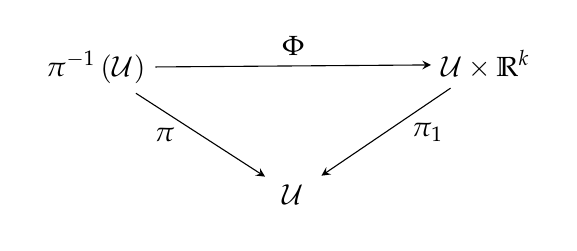
\begin{tikzpicture}
			\matrix (m) [matrix of math nodes,row sep=3em,column sep=4em,minimum width=2em]
			{
				\pi^{-1}\left(\sU \right)  & & \sU \times \R^k \\ 
				& \sU & \\};
			\path[-stealth]
			(m-1-1) edge node [above] {$\Phi$} (m-1-3)
			(m-1-1) edge node [left]  {$\pi~~$} (m-2-2)
			(m-1-3) edge node [right] {$~~\pi_1$} (m-2-2);
		\end{tikzpicture}
		\\ 	
		and the restriction of $\Phi$ to $E_p$ is a linear isomorphism from $E_p$ to $\{p\}\times \R^k \xrightarrow{\approx } \R^k$. (Here $\pi_1$ is the projection on the first factor).
	\end{enumerate}
	The manifold $E$ is called the \textit{total space} of the bundle, $M$ is called its \textit{base}, and $\pi$ is its \textit{projection}. Each map $\Phi$ in the above definition is called
	a \textit{local trivialization} of $E$  with base  $\sU$. 
	
\end{definition}

\begin{definition}\label{top_sm_sec_defn}\cite{lee:smooth_manifolds}
	Let $E$ be a smooth vector bundle  with base  a smooth manifold $M$, with projection $\pi: E\to M$. A section of $E$ is a \textit{section} of the map $\pi$, i.e., a continuous map $\sigma: M \hookto E$ such that $\pi\circ\sigma = \Id_M$. If $\sU \subset M$ is an open subset, a
	section of the restricted bundle $E|_{\sU}$ is called a \textit{local section} of $E$. A \textit{smooth
		section} is a (local or global) section that is smooth as a map between manifolds.
\end{definition}
\begin{remark}
	The definitions \ref{top_sm_bundle_defn} and \ref{top_sm_sec_defn} are specializations of \ref{top_vb_defn} and \ref{top_vb_cs_defn} ones.
\end{remark}


\begin{definition}\label{dg_prinicipal_defn}\cite{kobayashi_nomizu:diff_geom}
	Let $M$ be a manifold and $G$ is a Lie group. A (\textit{differential}) \textit{principal bundle over $M$ with group} $G$ consists of a manifold $P$ and an action of $G$ on $P$ satisfying the following conditions:
	\begin{enumerate}
		\item[(a)]  $G$ acts freely on $P$ on the right: 
		$$
		\left(u, a \right) \in P \times G\quad  ua = R_a u \in P;	
		$$
		\item[(b)] $M$ is the quotient space of $P$ by the equivalence relation induced by $G$, $M = P/G$, and the canonical projection $\pi: P \to M$  is differentiable;
		\item[(c)] $P$ is locally trivial, that is, every point $x$ of $M$ has neighbourhood $\sU$ such that there is a diffeomorphism  $\psi: \pi^{-1}\left(\sU
		\right) \cong \sU \times G$ such that $\psi\left(u\right)= \left( \pi\left(u\right), \varphi\left(u\right)\right)$  where $\varphi$ is a mapping of $\pi^{-1}\left(\sU
		\right)$ into $G$ satisfying $\varphi\left(ua\right)= \left( \varphi\left(u\right)\right) a$ for all $u \in \pi^{-1}\left(\sU
		\right)$ and $a \in G$.
	\end{enumerate}
	A principal fibre bundle will be denoted by $P\left(M, G, \pi \right)$,  $P\left(M, G \right)$ or simply $P$. We call $P$ the \textit{total space} or the \textit{bundle space}, $M$ the \textit{base space}, $G$ is the \textit{structure group} and $\pi$ the \textit{projection}. For each $x \in M$ $\pi^{-1}\left(x \right)$ is a closed manifold of $P$, called the \textit{fibre} over $x$. 
\end{definition}

\begin{empt}\label{dg_assoc_empt}\cite{kobayashi_nomizu:diff_geom}
	Let $P\left(M, G \right)$ be a principal fibre bundle  and $F$ is a manifold on which $G$ acts of the left: $\left(a, \xi \right) \in G \times F \mapsto a\xi \in F$.  On the product manifold $P\times F$, we let $G$ on right as follows: an element $a \in G$ maps $\left( u, \xi \right) \in P\times F$ into $\left( u a, a^{-1}\xi\right) \in P \times F$. The quotient space of $P \times F$ by group action is denoted by $E \bydef P\times_G F$ which has a natural differential structure. $E$ is a is a locally trivial bundle and  the  
	tuple $\left(E, M, F, G, P \right)$ is the \textit{bundle associated with $P$  with standard fibre $F$}.
\end{empt}


\
\section{Riemannian manifolds}
\begin{definition}\label{riemann_mani_defn}\cite{do_carmo:rg}
	%2.1 Definition.
	A \textit{Riemannian metric} (or \textit{Riemannian structure}) 
	on a differentiable manifold $M$ is a correspondence which associates 
	to each point $p$ of $M$ an inner product $\left\langle \cdot, \cdot\right\rangle_p$ (that is, a symmetric, 
	bilinear, positive-definite form) on the tangent space $T_pM$, which 
	varies differentiably in the following sense: If $\mathbf{x}: \sU \cong \R^n \to M$ 
	is a system of coordinates around $p$, with $\mathbf{x}\left(x_1,..., x_n\right) = q \in  \mathbf{x}\left(\sU\right)$
	and $\frac{\partial q}{\partial x_j}= d\mathbf{x}\left( 0,..., 1,...,0\right) $, 
	then
	\be\label{riemann_mani_eqn}
	\left\langle \frac{\partial}{\partial x_j} q, \frac{\partial}{\partial x_k} q\right\rangle_p= g_{jk}\left(x_1,..., x_n \right) 
	\ee
	is a differentiable function on $\sU$. 	It is clear this definition does not depend on the choice of 
	coordinate system. 
	%	Another way to express the differentiability of the Rieman	nian metric is to say that for any pair of vector fields X and , which 	are differentiable in a neighbourhood V of M, the function (X, Y) is 	differentiable on V. It is immediate that this definition is equivalent 	to the other. 	It is usual to delete the index p in the function ( , )p when- 	ever there is no possibility of confusion. The function gij (= ) is 	called the local representation of the Riemannian metric (or "the gij 	of the metric") in the coordinate system x: U  Rn   M. 
	A differentiable manifold with a given Riemannian metric will be called a \textit{Riemannian manifold}. 
	
\end{definition}
\begin{remark}\label{riemann_mani_rem}
	The Riemannian metric is completely defined by the \textit{metric tensor} $\left[g_{jk}\right]$ (cf. equation \eqref{riemann_mani_eqn})
\end{remark}


\begin{prop}\label{comm_cov_mani_prop}(Proposition 5.9 \cite{kobayashi_nomizu:diff_geom})
	\begin{enumerate}
		\item[(i)] Given a connected manifold $M$ there is a unique (unique up to isomorphism) universal covering manifold, which will be denoted by $\widetilde{M}$.
		\item[(ii)] The universal covering manifold $\widetilde{M}$ is a principal fibre bundle over $M$ with group $\pi_1(M)$ and projection $p: \widetilde{M} \to M$, where $\pi_1(M)$ is the first homotopy group of $M$.
		\item[(iii)] The isomorphism classes of covering spaces over $M$ are in 1:1 correspondence with the conjugate classes of subgroups of $\pi_1(M)$. The correspondence is given as follows. To each subgroup $H$ of $\pi_1(M)$, we associate $E=\widetilde{M}/H$. Then the covering manifold $E$ corresponding to $H$ is a fibre bundle over $M$ with fibre $\pi_1(M)/H$ associated with the principal bundle  $\widetilde{M}(M, \pi_1(M))$. If $H$ is a normal subgroup of $\pi_1(M)$, $E=\widetilde{M}/H$ is a principal fibre bundle with group $\pi_1(M)/H$ and is called a regular covering manifold of $M$.
	\end{enumerate}
\end{prop}

\begin{empt}\label{covering_metric_empt}
	If $\widetilde{M}$ is a covering space of a Riemannian manifold $M$ then it is possible to give $\widetilde{M}$ a Riemannian structure such that $\pi: \widetilde{M} \to M$ is a local isometry (this metric is called the {\it covering metric}) cf. \cite{do_carmo:rg} for details.
\end{empt}


\section{Differential operators on manifolds}
\begin{definition}\label{do_man_defn}\cite{kahn:glo_an}
	%Definition 6.1 
	Given an $n$-dimensional smooth manifold $M$ and two
	smooth, complex vector bundles  with base  $M$, say
	$\left(E_1, M, p_1\right)$ and $\left(E_1, M, p_1\right)$,
	let $ \Ga^\infty\left(M, E_j \right)$  be the complex vector space of sections of the bundle
	$\left(E_j, M, p_j\right)$, i.e., smooth maps $s:M \to E_j$ such that $\pi_j\circ s=\Id_{M}$.
	A \textit{linear differential operator} means a linear map of vector spaces
	$$
	P: \Ga^\infty\left(M, E_1 \right)\to \Ga^\infty\left(M, E_2 \right)
	$$
	such that $\supp P(s) \subset  \supp s$. We denote by 
	\be\label{do_man_eqn}
	D\left(M, E_1, E_2 \right)
	\ee
the space of all differential operators $\Ga^\infty\left(M, E_1 \right)\to \Ga^\infty\left(M, E_2 \right)$.
\end{definition}
\begin{remark}\label{do_man_rem}
If $E_1 = E_2= E$ then we denote
\be\label{do_man_alg_eqn}
	D\left(M, E \right)\bydef 	D\left(M, E, E \right).
\ee
The space $D\left(M, E \right)$ is an algebra over $\C$ with the given by the composition of operators product.
\end{remark}
\begin{definition}\label{do_man_order_defn}\cite{kahn:glo_an}
	%Definition 6.2
	Let $M$ be a smooth manifold, $x_0\in M$. Let $E_1$, $E_2$ be two
	smooth vector bundles with base  $M$, and let
	$$
	P:  \Ga^\infty\left(M, E_1 \right)\to  \Ga^\infty\left(M, E_2 \right)
	$$
	be a linear differential operator, in the sense of Definition \ref{do_man_defn}.
	Then we say that $P$ \textit{has order} $m$ at the point $x_0$ if $m$ is the largest non-negative
	integer such that there is some $s \in  \Coo\left(M, E_1 \right)$ and some smooth function
	$f$ defined in an open neighbourhood of $x_0$ and vanishing at $x_0$ such that $P(f^ms)(x_0)\neq0$.
	The order of $P$ is the maximum of the orders of $P$ at all the points of $M$. 
\end{definition}

\section{Distributions on manifolds}
\paragraph*{}
The notion of a distribution on smooth manifold $M$ is explained in 6.3.3 \cite{horm:I} and the space of distributions  is denoted by $\mathscr{D}'\left( M\right)$.
However $\mathscr{D}'\left( M\right)$ is not equal to the space of linear forms  $C_c\left( M\right) \cap \Coo\left(M \right)\to \C$.
\begin{definition}\label{top_distr_dens_def}
	If $M$ is a smooth manifold then a $\C$-valued linear form  $\Coo_c \left(M  \right)\bydef C_c\left( M\right) \cap \Coo\left(M \right)\to\C$ is said to be a \textit{distribution density}. The space of distribution densities will be denoted by $\Coo_c \left(M  \right)'$. Denote by 
	\be\label{top_distr_dens_eqn}
	\begin{split}
	\left\langle \cdot, \cdot \right\rangle : \Coo_c \left(M  \right)'\times \Coo_c \left(M  \right) \to \C,\\
\left\langle \phi, a \right\rangle \bydef \phi\left(a \right) 
	\end{split}
	\ee
	the natural pairing.
\end{definition}
\begin{remark}
The space $\mathscr{D}'\left( M\right)$ is relevant to $\Coo_c \left(M  \right)'$ one (cf. \cite{horm:I})
\end{remark}
\begin{remark}
	If there is a positive measure $\mu$ on $M$ which is locally presented by a $\dim M$-dimensional external differential form then there is the natural inclusion
	\be
	\begin{split}
		C\left(M \right) \subset \Coo_c \left(M  \right)',\\
		f \mapsto \left( \phi \mapsto  \int_M f \phi d \mu \right) .
	\end{split}
	\ee
\end{remark}
\begin{remark}
	From $\Coo \left(M  \right) \Coo_c \left(M  \right)\subset \Coo_c \left(M  \right)$ it follows that there is the action $\Coo \left(M  \right)\times \Coo_c \left(M  \right)' \to \Coo_c \left(M  \right)'$ given by
	\bean
	\langle ab, c\rangle \bydef \langle b, ac\rangle\quad a \in \Coo \left(M  \right), \quad b \in \Coo_c \left(M  \right)', \quad c \in \Coo_c \left(M  \right).
	\eean
	where 	$\langle \cdot , \cdot \rangle: \Coo_c \left(M  \right)'\times \Coo_c \left(M  \right)\to\C$ is the natural pairing.
\end{remark}
\begin{remark}\label{top_distr_dens_q_rem}
	From the pairing $\Coo \left(M  \right)\times \Coo_c \left(M  \right)' \to \Coo_c \left(M  \right)'$ it turns out that a pair $\left(\Coo_c \left(M  \right)', \Coo \left(M  \right)\right)$ is a quasi $*$-algebra (cf. Definition \ref{quasi_defn}).
\end{remark}


% \begin{theorem}
%6.28 Theorem 
%Suppose $\La \in \mathscr D'\left(\Om\right)$. There exist continuous functions $g_\a$ in $\Om$, one for each multi-index $\a$, such that 
% \begin{enumerate}
% 	\item[(a)] each compact $K \subset \Om$ intersects the supports of only finitely many $g_\a$, and
% 	\item[(b)] $\La = \sum_\a D^\a g_a$.
% \end{enumerate}
% 	If $\La$ has finite order, then the functions $g_\a$ can be chosen so that only 
% 	finitely many are different from $0$. 
%\end{theorem}



	\section{Flat connections}\label{geom_flat_subsec}
\paragraph*{}
Here I follow to \cite{kobayashi_nomizu:diff_geom}. Let $M$ be a manifold and $G$ a Lie group. A (\textit{differentiable}) \textit{principal bundle over M with group} $G$ consists of a manifold $P$ and an action of $G$ on $P$ satisfying the following conditions:
\begin{enumerate}
	\item [(a)] $G$ acts freely on $P$ on the right: $\left(u, a \right) \in P \times G \mapsto ua = R_au \in P$;
	\item[(b)] $M$ is the quotient space of $P$ by the equivalence relation induced by $G$, i.e. $M = P/G$, and the canonical projection $\pi: P \to M$ is differentiable;
	\item[(c)] $P$ is locally trivial, that is, every point $x$ of $M$ has an open neighbourhood $U$ such that $\pi^{-1}\left( U\right)$ is isomophic to  $U\times G$ in the sense that there is a diffeomorphism $\psi:  \pi^{-1}\left( U\right) \to U \times G$ such that $\psi\left( u\right) = \left( \pi\left( u\right), \varphi\left(u \right) \right) $ where $\varphi$ is a mapping of $\pi^{-1}\left(U \right)$ into $G$ satisfying  $\psi\left(ua \right)= \left( \psi\left( u\right)\right) a$  for all $u \in \pi^{-1}\left(U \right)$ and $a \in G$. 
\end{enumerate}
A principal fibre bundle will be denoted by $P\left( M, G, \pi\right), ~ P\left(M, G \right)$ or simply $P$.
\paragraph*{} Let $P\left(M, G \right)$ be a principal fibre bundle over a manifold with group $G$. For each $u \in P$ let $T_u\left(P \right)$ be a tangent space of $P$ at $u$ and $G_u$ the subspace of $T_u\left( P\right)$ consisting of vectors tangent to the fibre through $u$. A \textit{connection} $\Ga$   in $P$ is an assignment of a subspace $Q_u$ of $T_u\left(P \right)$ to each $u \in P$ such that
\begin{enumerate}
	\item [(a)] $T_u\left(P \right) = G_u \oplus Q_u$ (direct sum);
	\item[(b)] $Q_{ua}= \left(R_a \right)_*Q_u$ for every $u \in P$ and $a \in G$, where $R_a$ is a transformation of $P$ induced by $a \in G, ~ R_au=ua$.
\end{enumerate}
\paragraph*{}
Let $P = M \times G$ be a trivial principal bundle. For each $a \in G$, the set $M \times \{a\}$ is a submanifold of $P$. The \text{canonical flat connection} in $P$ is defined by taking the tangent space to $M \times \{a\}$ at $u = \left(x, a \right)$ as the horizontal tangent subspace at $u$. A connection in any principal bundle is called \textit{flat} if every point has a neighbourhood such that the induced connection in $P|_U = \pi^{-1}\left(U \right)$ is isomorphic with the canonical flat connection.

\begin{cor}\label{dg_flat_cor}(Corollary II 9.2 \cite{kobayashi_nomizu:diff_geom})
	Let $\Ga$ be a connection in $P\left(M, G \right)$ such that the curvature vanishes identically. If $M$ is paracompact and simply connected, then $P$ is isomorphic to the trivial bundle and $\Ga$ is isomorphic to the canonical flat connection in $M \times G$.
\end{cor}
\begin{remark}
	The \textit{curvature} notion is explained in \cite{kobayashi_nomizu:diff_geom}.
\end{remark}
\paragraph*{}

If $\widetilde{\pi}: \widetilde{M} \to M$ is a covering then the $\widetilde{\pi}$-\textit{lift} of $P$ is a principal $\widetilde{P}\left(\widetilde{M}, G \right)$  bundle, given by
\be\nonumber
\widetilde{P} = \left\{\left(u, \widetilde{x}\right) \in P \times \widetilde{M}~|~ \pi\left(u \right) = \widetilde{\pi}\left( \widetilde{x}\right) \right\}.
\ee
If $\Ga$ is a  connection on $P\left( M, G\right)$ and $\widetilde{M} \to M$ is a covering then is a canonical connection $\widetilde{\Ga}$ on $\widetilde{P}\left(\widetilde{M}, G \right)$ which is the \textit{lift} of $\Ga$, that is, for any $\widetilde{u} \in \widetilde{P}$ the horizontal space $\widetilde{Q}_{\widetilde{u}}$ is isomorphically  mapped onto the horizontal space $Q_{\widetilde{\pi}\left(\widetilde{u} \right) }$ associated with the connection $\Ga$.
If $\Ga$ is flat then from the Proposition (II 9.3 \cite{kobayashi_nomizu:diff_geom}) it turns out that there is a covering $\widetilde{M} \to M$ such that $\widetilde{P}\left(\widetilde{M}, G \right)$ (which is the lift of $P\left(M,G\right)$) is a trivial bundle, so the lift $\widetilde{\Ga}$ of $\Ga$ is a canonical flat connection (cf. Corollary \ref{dg_flat_cor}). From the the Proposition (II 9.3 \cite{kobayashi_nomizu:diff_geom}) it follows that for any flat connection $\Ga$  on $P\left(M, G \right)$ there is a group homomorphism $\varphi: G\left( \widetilde{M} ~|~ M\right) \to G$ such that
\begin{enumerate}
	\item [(a)] There is an action $G\left( \widetilde{M} ~|~ M\right) \times \widetilde{P} \to \widetilde{P} \approx \widetilde{M} \times G$ given by
	\be\label{nontriv_buble_eqn}
	g \left(\widetilde{x}, a \right) = \left( g\widetilde{x}, \varphi\left( g\right) a\right); \quad \forall \widetilde{x} \in \widetilde{M}, ~ a \in G, 
	\ee
	\item[(b)] There is the canonical diffeomorphism  $P = \widetilde{P}/G\left( \widetilde{M} ~|~ M\right)$,
	\item[(c)] The lift $\tilde{\Ga}$ of $\Ga$ is a canonical flat connection.
\end{enumerate}

\begin{defn}
	In the above situation we say that the flat connection $\Ga$ is \textit{induced} by the covering $\widetilde{M}\to M$ and the homomorphism $G\left( \left.\widetilde{M}~\right|M\right) \to G$, or we say that $\Ga$ \textit{comes from} $G\left( \left.\widetilde{M}~\right|M\right) \to G$.
\end{defn}
\begin{remark}
	The  Proposition (II 9.3 \cite{kobayashi_nomizu:diff_geom}) assumes that $\widetilde{M} \to M$ is the universal covering however it is not always necessary requirement.
\end{remark}
\begin{remark}
	If $\pi_1\left(M, x_0 \right)$ is the fundamental group \cite{spanier:at} then there is the canonical surjective homomorphism $\pi_1\left(M, x_0 \right) \to G\left( \left.\widetilde{M}~\right|M\right)$. So there exist the composition $\pi_1\left(M, x_0 \right) \to G\left( \left.\widetilde{M}~\right|M\right) \to G$. It follows that any flat connection comes from the homomorphisms $\pi_1\left(M, x_0 \right) \to G$. 
\end{remark} 
\paragraph*{}
Suppose that there is the right action of $G$ on $P$ and suppose that $F$ is a manifold with the left  action of $G$. There is an action of $G$ on $P \times F$ given by $a\left( u, \xi\right) = \left(u a, a^{-1}\xi \right)$ for any $a \in G$ and $\left( u, \xi\right) \in P\times F$. The quotient space $P \times_G F = \left(P \times F \right)/G$ has the natural structure of a manifold and if $E =  P \times_G F$ then\\ $E\left(M, F, G, P \right)$ is said to be the \textit{fibre bundle over the base $M$, with (standard) fibre $F$, and (structure) group G which is associated with the principal bundle P} (cf. \cite{kobayashi_nomizu:diff_geom}). If $P = M \times G$ is the trivial bundle then $E$ is also trivial, that is, $E = M \times F$. If $F = \C^n$ is a vector space and the action of $G$ on $\C^n$ is a linear representation of the group then $E$ is the linear bundle. Denote by $T\left(M \right)$ (resp. $T^*\left(M \right)$) the tangent  (resp. contangent) bundle, and denote by $\Ga\left( E\right)$, $\Ga\left(T\left(M \right)\right)$, $\Ga\left(T^*\left(M \right)\right)$ the spaces of sections of $E$, $T\left(M \right)$, $T^*\left(M \right)$ respectively. Any connection $\Ga$ on $P$ gives a covariant derivative  on $E$, that is,
for any section  $X \in \Ga\left( T\left(M \right)\right) $ and any section $\xi \in \Ga\left( E\right)$ there is the derivative given by
\be\nonumber
\nabla_X\left( \xi\right) \in \Ga\left( E\right).
\ee
If $E = M \times \C^n$, $\Ga$ is the canonical flat connection and $\xi$ is a trivial section, that is, $\xi = M \times \{x\}$ then 
\be\label{comm_triv_eqn}
\nabla_X \xi = 0,~~ \forall X \in T\left(M \right).
\ee
For any connection there is the unique map
\be\label{comm_alg_conn}
\nabla : \Ga\left( E\right) \to \Ga\left( E \otimes T^*\left( M\right) \right)
\ee
such that
\be\nonumber
\nabla_X \xi = \left(\nabla \xi, X \right)
\ee
where the pairing $\left(\cdot, \cdot\right) : \Ga\left( E \otimes T^*\left( M\right) \right) \times \Ga\left( T\left( M\right)\right)  \to \Ga\left( E \right) $ is induced by the pairing $\Ga\left( T^*\left(M \right)\right)   \times \Ga\left( T\left( M\right)\right)  \to \Coo\left(M \right) $.

\chapter{Algebra}
\section{Groups}\label{grops_sec}
\paragraph{}
We suppose that the reader is familiar  with the notion of group. Here I follow to \cite{lang}.
Let $G$ be a group and $H$ a subgroup. A \textit{left  coset} of $H$ in $G$ is a subset of 
$G$ of type $aH$, for some element $a \in G$. 
$G$ is the disjoint union of the left  cosets of $H$. A similar 
remark applies to right cosets (i.e. subsets of $G$ of type $Ha$). The number of left  
cosets of $H$ in $G$ is denoted by $(G : H)$, and is called the \textit{(left) index} of $H$ in $G$. The kernel of a group-homomorphism is a 
subgroup. We now wish to characterize such subgroups. 
Let $f: G' \to G$ be a group-homomorphism, and let $H$ be its kernel. If $x$ is an 
element of $G$, then
$xH = Hx$ .

	\begin{definition}\label{normal_subgroup_defn}\cite{kurosh:lga}
	A subgroup $H$ is called a \textit{normal subgroup} (or \textit{invariant subgroup}) of the group $G$, if the left-sided partition of the group $G$
	with respect to the subgroup $H$ coincides with the right-sided
	partition, i.e. if for every $g\in G$ the equation
	\be\label{normal_subgroup_eqn}
	gH = Hg
	\ee
	or equivalently
	\be\label{normal_subgroup_ghg_eqn}
	gHg^{-1} = H
	\ee
	holds (understood in the sense that the two subsets coincide in $G$).
	Thus we can speak simply of \textit{the partition of the group} $G$ \textit{with
		respect to the normal subgroup} $H$.
\end{definition}
The left index of any normal subgroup coincides with the right one.
\begin{definition}\label{group_coset_defn}\cite{lang}
Let $A$ be a group and $H$ a subgroup. A \textit{left  coset} of $H$ in $G$ is a subset of $G$ of type $aH$ for some $a\in G$. An element of $aH$ is called a \textit{coset representative} of $aH$. Similarly we define \textit{right cosets} $Ha$.
\end{definition}
\begin{definition}\label{group_inv_lim_defn}\cite{lang}
If $\left\{G_\a\right\}$ is an inverse system of
groups  (that is, $G_\a$ is a group for each $\a$ and $f^\bt_\a: G_\bt\to  G_\a$ is a homomorphism 
for $\a\le \bt$), their \textit{inverse limit} $\varprojlim G_\a$ (which is a set (cf. Definition \ref{inverse_limit_defn})) is a subgroup of $\prod G_\a$. 
\end{definition}
\begin{definition}\label{simple_group_defn}
A group $G$ is said to be \textit{simple} if it is non-trivial, and has no normal subgroups 
other than $\{e\}$ and $G$ itself. 

\end{definition}
\begin{theorem}\cite{lang}\label{jordan_holder_thm}
%Theorem 3.5. 
(Jordan-Holder) Let $G$ be a group, and let
$$ 
G = G_1 \supset ...\supset G_r\subset \left\{e\right\}
$$
be a normal tower such that each group $G_j / G_{j+1}$ is simple, and $G_j \neq G_{j+1}$
for $j = 1...r$. Then any other normal tower of $G$ having the same properties is equivalent to this one.
\end{theorem}

\begin{example}\label{profinite_exm}\cite{lang}
%Example. 
Let $G$ be a group. Let $\F$ be the family of normal subgroups of 
finite index. If $H$, $K$ are normal of finite index, then so is $H \cap K$ so ($\F$ is a 
directed family. We may then form the inverse limit $\varprojlim G/H$ with $H \in \F$
A group which is an inverse limit of finite groups is called \textit{profinite}. It is the \textit{profinite completion} of $G$.

\end{example}
\subsection{Finitely generated Abelian groups}\label{alg_fin_gen_ab_sec}
\paragraph{}
Here I follow to \cite{lang}.
Let $A$ be an Abelian group. An element $a \in A$ is said to be a \textit{torsion} element 
if it has finite period. The subset of all torsion elements of $A$ is a subgroup of $A$ 
called the \textit{torsion subgroup} of $A$. 
The torsion subgroup of $A$ is denoted by $A_{\mathrm{tor}}$.
A finitely generated torsion Abelian group is obviously finite.  If A is an Abelian group and $p$ a prime number, 
we denote by $A(p)$ the subgroup of all elements $x\in A$ whose period is a power 
of $p$. Then $A(p)$ is a torsion group, and is a $p$-\textit{group} if it is finite. 
\begin{theorem}\label{alg_fin_gen_ab_fin_thm}\cite{lang}
%Theorem 8.1 
Let $A$ be a torsion Abelian group. Then $A$ is the direct sum of 
its subgroups $A(p)$ for all primes $p$ such that $A(p)\neq\{0\}$. 
\end{theorem}
A finite $p$-group A is said to be of {type} $\left(p^{r_1}, ...,p^{r_s} \right)$ 
if $A$ is isomorphic to the product of cyclic groups of orders $p^{r_j}~ (j = 1,..., s)$.
\begin{theorem}\label{alg_finp_gen_ab_fin_thm}\cite{lang}
%Theorem 8.2. 
Every finite Abelian $p$-group is isomorphic to a product of 
cyclic $p$-groups. If it is of type $\left(p^{r_1}, ...,p^{r_s} \right)$ with 
$$
r_1 \ge r_2\ge ...\ge r_s
$$
then the sequence of integers $\left( r_1,..., r_s\right)$  is uniquely determined.
\end{theorem}
\begin{theorem}\label{alg_fin_gen_ab_inf_thm}\cite{lang}
%Theorem 8.5. 
Let A be a finitely generated Abelian group, and let $A_{\mathrm{tor}}$ be 
the subgroup consisting of all elements of $A$ having finite period. Then $A_{\mathrm{tor}}$ is 
finite, and $A/A_{\mathrm{tor}}$ is free. There exists a free subgroup $B$ of $A$ such that $A$ is the 
direct sum of $A_{\mathrm{tor}}$ and $B$. 
\end{theorem}


	\section{Finitely generated modules}
	\begin{theorem}\label{fin_gen_thm}\cite{kasch:mr}
		% 2.3.13 THEOREM. T
		The module $M_R$ over an (unital) ring $R$ is finitely generated if and only if for every set $\left\{A_\la\right\}_{\la\in\La}$ of submodules $A_\la\hookto  M$ with 
		$$
		M=\sum_{\la \in \La} A_\la
		$$
		there is a finite subset $\La_0\subset \La$  such that 
		$$
		M = \sum_{\la \in \La_0} A_\la.
		$$
	\end{theorem}

	\section{Algebraic Morita equivalence}
	
	\begin{defn}\label{morita_ctx_defn}
		A \textit{Morita context} $\left( A,B,P,Q,\varphi,\psi\right)$ or, in some authors (e.g. Bass \cite{bass}) the \textit{pre-equivalence data} is a generalization of Morita equivalence between categories of modules. In the case of right modules, for two associative $\mathbf{k}$-algebras (or, in the case of $\mathbf{k} = \mathbb{Z}$, rings) $A$ and $B$, it consists of bimodules $_AP_B$, $_BQ_A$ and bimodule homomorphisms $\varphi: P\otimes_B Q\to A$, $\psi: Q\otimes_A P\to B$ satisfying mixed associativity conditions, i.e. for any $p,p' \in P$ and $q,q' \in Q$ one  has:
		\begin{equation}\label{morita_ctx_eqn}
			\begin{split}
				\varphi\left(p\otimes q \right) p' = p \psi\left(q\otimes p' \right),\\
				\psi\left(q \otimes p \right) q' = q\varphi\left(p\otimes q' \right).  
			\end{split}
		\end{equation}
		A Morita context is a \textit{Morita equivalence} if both $\varphi$ and $\psi$ are isomorphisms of bimodules. 
	\end{defn}
	
	\begin{rem}\label{morita_rem}
		The Morita context $\left( A,B,P,Q,\varphi,\psi\right)$  is a Morita equivalence if and only if $A$-module $P$ is a finitely generated projective generator (cf. \cite{bass} II 4.4).
	\end{rem}
	
	% \begin{cordefn}\label{invert_mod_defn}\cite{bass}
	% 	Let $R$ be a commutative ring, and let $A$, $B$ be $R$-algebras
	% 	We call a left  $A\otimes_RB^\circ$ module $M$ \textit{invertible} if it satisfies to the following conditions, which are equivalent:
	% 	\begin{enumerate}
	% 		\item [(a)] $\otimes_{A}M:~ mod$-$A \xrightarrow{\approx} mod$-$B$ is an equivalence.
	% 		\item[(b)] There is a left  left  $B\otimes_RA^\circ$ module $N$ such that $M\otimes_BN \cong A$ and $N\otimes_AM \cong B$ as bimodules.
	% 		\item [(c)] $M\otimes_{B}:~B$-$mod \xrightarrow{\approx} ~B$-$mod$ is an equivalence.
	% 	\end{enumerate}
	%\end{cordefn}
	% \begin{empt}\label{invert_mod_auto_empt}\cite{bass}
	% 	For any $R$-algebra $A$ write $\mathbf{Pic}_R\left(A \right)$  for the category of invertible $A\otimes_RA^\circ$ modules and bimodule isomorphisms. For any $\al, \bt \in \Aut_{R\mathrm{-alg}}\left(A \right)$ denote by $_\al A_\bt$ the $A\otimes_RA^\circ$ module such that there is $R$-linear isomorphism $\varphi: A \xrightarrow{\approx}_\al A_\bt$ and following condition holds
	% 	\be\label{pic_act_eqn}
	% 	a\varphi\left(x \right)b = \varphi\left(\al\left(a \right) x\bt\left(b\right)  \right); \quad \forall a, x, b \in A. 
	% 	\ee	
	% \end{empt}
	
	% \begin{proposition}\label{invert_mod_auto_prop}
	% 	Let $A$ be an $R$-algebra and let  $\al, \bt, \ga \in \Aut_{R\mathrm{-alg}}\left(A \right)$.
	%	\begin{enumerate}
	%		\item [(i)] $_\al A_\bt \cong _{\ga\al} A_{\ga\bt}$ as bimodules.
	% 		\item[(ii)] $_{\Id_A} A_{\al}\otimes_A ~_{\Id_A} A_{\al} \cong _{\Id_A} A_{\al\bt}$ as bimodules.
	% 		\item[(iii)] 
	% 		$$
	% 		_{\Id_A} A_{\al} \cong _{\Id_A}A_{\Id_A} \Leftrightarrow \al \mathrm{~is~an~inner~automorphism}.
	% 		$$
	%		\item[(iv)] If $P \in \mathbf{Pic}_R\left(A \right)$ and if $P\cong A$ as left  $A$-modules then $P\cong _{\Id_A} A_{\al}$ as bimodules for some $\al \in  \Aut_{R\mathrm{-alg}}\left(A \right)$.
	% 	\end{enumerate}
	% \end{proposition}
	\begin{definition}\label{progenerator_defn}\cite{af:rings_cat_mod}
	A left $R$-module $_RP$ is a \textit{progenerator} (or a \textit{left} $R$-\textit{progenerator}) in case it is a finitely generated projective generator. In particular, $_RR$ is a progenerator. 
Indeed, $_RP$ is a progenerator if and only if there are integers $m$ and $b$ and 
modules $P'$ and $R'$ with 
\be\label{progenerator_eqn}
R^m \cong P\oplus P'\quad P^m = R \oplus  R'
\ee
\end{definition}
\begin{theorem}\cite{af:rings_cat_mod}
%	22.1. Theorem. 
Let $R$ and $S$ be equivalent rings via inverse equivalences $F:_R\mathscr{M}\xrightarrow{\cong}_S\mathscr{M}$ and $G:_S\mathscr{M}\xrightarrow{\cong}_R\mathscr{M}$. Set
$$
P \bydef F\left( R\right) \quad \text{and} \quad Q \bydef G\left(  S\right) 
$$
Then $P$ and $Q$ are naturally bimodules $_SP_R$ and $_RQ_S$ such that 
\begin{enumerate}
	\item[(i)] $_SP_R$ and $_RQ_S$ are faithfully balanced; 
\item[(ii)] $P_R$, $_SP$, $_RQ$ and $Q_S$ are all progenerators; 
\item[(iii)] $_SP_R \cong \Hom_S\left(Q,S\right)\cong \cong \Hom_R\left(Q,R\right)$ and $_RQ_S \cong \Hom_R\left(P,R\right)\cong \cong \Hom_S\left(P,S\right)$;
\item[(iv)]  $F \cong \Hom_R\left(Q,- \right)$ and  $G \cong \Hom_S\left(P, - \right)$;
\item [(v)]  $F \cong \left( P\otimes_R -\right)$ and  $GT \cong \left( Q\otimes_S -\right)$.
		 
\end{enumerate}

\end{theorem}

\begin{theorem}\label{progenerator_morita_thm}\cite{af:rings_cat_mod}
	%	22.2. Theorem. 
Let $R$ and $S$ be rings and let
$$
F : _R\mathscr{M}\to _S\mathscr{M}\quad \text{and} \quad G : _S\mathscr{M}\to _M\mathscr{M}
$$ 
be additive functors, where both $_R\mathscr{M}$ and $_S\mathscr{M}$ a categories of left $R$- and $S$-modules respectively. Then $F$ and $G$ are inverse equivalences if and only if there 
exists a bimodule $_SP_R$ such that: 
	\begin{enumerate}
		\item[(i)]	$_SP$ and $P_R$ are progenerators; 
	\item[(ii)]	 $_SP_R$ is balanced; 
		\item[(iii)]	 $F \cong \left( P\otimes_R-\right) $ and $G \cong \Hom_S\left( P, -\right)$. 
		
	\end{enumerate}
	Moreover , if there is a bimodule $_SP_R$ satisfying these conditions, then with 
	$$Q \bydef \Hom_R \left(P, R \right),$$ 
	we have $_RQ_S$ with $_RQ$ and $Q_S$ progenerators and 
	$$	
F \cong \Hom_R \left(Q, - \right)	\quad and \quad G \cong \left(Q\otimes_S - \right). 
$$
\end{theorem}
\begin{corollary}
%22.4. Corollary. 
For two rings R and S the following assertions are equivalent: 
\begin{enumerate}
	\item[(i)] $R$ is Morita equivalent to $S$.
	\item[(ii)] There is a progenerator $P_R$ with $S\cong  \End(P_R)$;
	\item[(iii)] There is a progenerator $_RQ$ with $S\cong  \End(_RQ)$.
\end{enumerate}

\end{corollary}
	
	\section{Finite Galois coverings and   Morita equivalence}\label{fin_gal_cov_sec}
	\paragraph*{} Here I follow to \cite{auslander:galois}, but used here notation is adopted to this book and   different from  \cite{auslander:galois} one. 
	Let $\widetilde \La$ be a ring and let $G$ be a finite group operating on  $ \La$ as a group of automorphisms.	Let $\widetilde \La\rtimes G$ be an algebra such that $\widetilde\La\rtimes G \approx \widetilde \La\times G$ as an Abelian group and a multiplication law is given by
	\be\label{croosed_prod_eqn}
\forall 	\left( \widetilde a, g\right),\left(\widetilde b, h\right)\in \widetilde \La\times G \quad 	\left( \widetilde a, g\right)\cdot \left(\widetilde b, h\right) =\left(\widetilde a\left(g \widetilde b \right), gh  \right).
	\ee
	Let us consider the category $\mathscr{M}^G_{\widetilde{\La}}$ of $G$-$\widetilde{\La}$ modules, i.e.  any object $M \in \mathscr{M}^G_{\widetilde{A}}$ is a $\widetilde{\La}$-module with equivariant action of $G$, i.e. for any $m \in M$ a following condition holds
	$$
	g\left(\widetilde{a}m \right)=  \left(g\widetilde{a} \right) \left(gm \right) \text{ for any } \widetilde{a} \in \widetilde{A}, ~ g \in G.
	$$
	Any morphism $\varphi: M \to N$ in the category $\mathscr{M}^G_{\widetilde{A}}$ is $G$- equivariant, i.e.
	$$
	\varphi\left( g m\right)= g \varphi\left( m\right)   \text{ for any } m \in M, ~ g \in G.
	$$
A left $\widetilde\La \rtimes G$-module $M$ may be thought of as a $G$-$\widetilde{\La}$-module, i.e. the category $\mathscr{M}_{\widetilde{\La}\rtimes G}$ of $\widetilde{\La}\rtimes G$- modules is equivalent to the $\mathscr{M}^G_{\widetilde{A}}$ one.
$$
\forall g \in G\quad \forall \widetilde a \in \widetilde \La\quad m \in M\quad g\left(am \right) = g\left(\widetilde a \right)g\left(m \right).
$$	
In the same way a	$\widetilde\La \rtimes G$-morphism between  $\widetilde\La \rtimes G$ modules $M$ and $N$ is a $\La$-morphism $f: M\to N$ such that $f\left(gm \right) = g\left( f\left(m \right)\right)$ for each $m \in M$ and $g\in G$. So a category
\begin{definition}\label{pregalois_defn}
We say that the action $G\times \widetilde\La \to \La$ is \textit{pregalois} if $\widetilde \La$ is a projective $ \widetilde\La\rtimes G$-generator where $\widetilde \La$ is considered as a left $\La\rtimes G$-module by
\be\label{croosed_prod_m_eqn}
\forall a, b \in \La \quad \forall g \in G \quad \left(a, g \right) \cdot b \bydef a. \left(g b \right) 
\ee
In this situation we say that the pair $\left(\La, G \right)$ is \textit{pregalois}. If 
$$
\La \bydef \widetilde{\La}^G \bydef \left\{\left. a \in  \widetilde{\La} \right| \forall g \in G \quad ga = a\right\}
$$
is a fixed point subring then we say that a pair $\left(\widetilde \La, \La\right)$ is \textit{pregalois}.
\end{definition} 
	When $G$ operates on $\widetilde\La$ as a group of automorphisms, the same action induces an action on $\widetilde \La^\circ$, the opposite ring of $A$.  The map
\bean
\begin{split}
	f: \widetilde \La \rtimes G \to \widetilde \La^\circ\rtimes G,\\
	\left(\widetilde a,g \right) \mapsto g\left(\widetilde a,g \right)g^{-1}
\end{split}
\eean
is easily seen to be an antiisomorphism. Hence with this map we may identify $\left( \widetilde \La \rtimes G \right)^\circ$ with $\widetilde \La^\circ \rtimes G$. 
For any $G$-$\widetilde{\La}$ module $M$  denote by
\bean
M^G \bydef \left\{m \in M | \forall g \in G \quad gm = m\right\}.
\eean


\begin{proposition}\cite{auslander:galois}
	\begin{enumerate}
		\item [(i)] The evaluation map 
		\bean
		\pi_M: \Hom_{\widetilde{\La}\rtimes G}\to M,\\
		f \mapsto f\left(1 \right) 
		\eean
	induces a functorial isomorphism $\Hom_{\widetilde{\La}\rtimes G}\xrightarrow{\cong } M^G$ for all $\widetilde{ \La }$-$G$ modules $M$.
	\item[(ii)] $\phi_{\widetilde \La} :\End_{\widetilde{\La}\rtimes G}\left(\widetilde\La \right)^\circ \to \widetilde \La^G$ is a ring isomorphism.
	\end{enumerate}
\end{proposition}
As a consequence of the isomorphism $\End_{\widetilde{\La}\rtimes G}\left(\widetilde\La \right)^\circ \cong \widetilde \La^G$ we have from general Morita theory (cf. Remark \ref{morita_rem}) the following connection between the category $\mathscr{M}_{\widetilde{\La}\rtimes G}$ of left $\widetilde{\La}\rtimes G$ modules, and $\mathscr{M}_{\widetilde{\La}^G}$, the category of $\widetilde{\La}^G$-modules, when $\left( \widetilde{\La},G\right)$ is pregalois.
\begin{proposition}\label{galois_morita_prop}\cite{auslander:galois}
$\left( \widetilde{\La},G\right)$ is pregalois if and only if $\widetilde \La\otimes_{\widetilde \La^G}-:\mathscr{M}_{\widetilde{\La}^G}\to \mathscr{M}_{\widetilde{\La}\rtimes G}$ and $\Hom_{\widetilde{\La}\rtimes G}: \left( \widetilde{\La}, -\right)$ are inverse equivalence of categories.
\end{proposition}
\begin{remark}\label{inverse_galois_rem}
There are left and right of $\widetilde{A} \rtimes G$ on $\widetilde{A}$ is given by
\begin{equation}\label{morita_ta_act_eqn}
	\begin{split}
		\forall \widetilde{a}\in \widetilde{\La}\quad \forall a \in \widetilde{\La} \rtimes G\quad a \widetilde{a} = \sum_{g \in G} a\left( g\right) \left( g\widetilde{a}\right)   , \quad
		\widetilde{a} a =\sum_{g \in G} g^{-1}\left(\widetilde{a} a\left( g\right)\right). \end{split}
\end{equation}
The left  (resp. right) action of $\La$ on $\widetilde{\La}$ we define as left  (resp. right) multiplication by $\La$.

 Otherwise in \cite{auslander:galois} it is proven that if $\widetilde{\La}$ is a finitely generated, projective $\La$-module then there is an  equivalence between a category $\mathscr{M}_{\La}$ of $\La$-modules and the category $\mathscr{M}_{\widetilde{\La}\left[ G\right]}$ (cf. Definition \ref{category_equivalence_definition}). It turns out that the category $\mathscr{M}^G_{\widetilde{\La}}$ is equivalent to the category $\mathscr{M}_{\La}$. The equivalence is given by mutually inversed functors $\left( -\right) \otimes \widetilde{\La}: \mathscr{M}_{\La} \to \mathscr{M}^G_{\widetilde{\La}}$ and $\left( -\right) ^G: \mathscr{M}^G_{\widetilde{\La}}\to \mathscr{M}_{\La}$.
\end{remark}
	\section{Topological and algebraic dual}\label{top_alg_dual_sec}
\paragraph{} For any locally compact Abelian group $G$  field one can define its \textit{topological dual} $G^*$ as a group of continuous  characters. For any vector space $V$ over a field $K$ there is \textit{algebraic dual} space $V'$ of $K$-linear functionals (cf. \cite{weil:basic_number_theory}).
\begin{theorem}\label{top_alg_thm}\cite{weil:basic_number_theory}
%THEOREM 3. 
Let $K$ be a non-discrete locally compact field, and $V$
a left vector-space of finite dimension $n$ over   $K$; let $\chi$ be a non-trivial
character of the additive group of $K$. Then the topological dual $V^*$ of $V$ is
a right vector-space of dimension $n$ over   $K$; the formula
$$
\left\langle v, v^* \right\rangle_V =  \chi\left(\left[v, v'\right] \right) 
$$
defines a bijective mapping $v' \mapsto v^*$ of the algebraic dual $V'$ of $V$ onto $V^*$.
%if x(xy)= I for all x, y in K, this mapping is an isomorphism for thestructures of I/ , V* as right vector-spaces over K.
\end{theorem}	

	
	
	\section{Profinite and residually finite groups}\label{profinite_section}
	\begin{empt}\label{prof_empt}\cite{dix:profinite}
		Let $G$ be a group and $\left\{G_\al \right\}$ be the set of all normal subgroups of finite index in $G$. Then the set $\left\{G/G_\al, \phi_{\al\bt}\right\}$ of finite quotients $G/G_\al$, of $G$ together with the canonical projections $\phi_{\al\bt}:G/G_\al \to G/G_\bt$  whenever $G_\al \subset G_\bt$ is an inverse system. The inverse limit $\varprojlim G/G_\a$ of this system is called the \textit{profinite completion} of $G$ and is denoted by $\widehat{G}$. The group $\widehat{G}$ can also be described as the closure of the image of $G$ under the
		the diagonal mapping $\Delta : G \to \prod \left( G/G_\a\right)$  where $G/G_\a$, is given the discrete topology and $\prod \left( G/G_\a\right)$ has the product topology. In this description the elements of $\widehat{G}$ are the
		elements $\left(g_\a \right) \in \prod \left( G/G_\a\right)$ which satisfy $\phi_{\al\bt}\left( g_\al\right)= \bt$  whenever $G_\a \subset G_\bt$.
	\end{empt} 
	%\begin{theorem}\label{profinite_thm}\cite{dix:profinite}
	%	Let $G$ and $H$ be finitely generated groups, and let $\widehat{G}$ (resp. $\widehat{H}$) be the profinite completion of $G$ (resp. $H$), Then $\widehat{G}$ and $\widehat{H}$ are isomorphic as topological groups id the set of isomorphism classes of finite quotients  of $G$ is equal the set of isomorphism classes of finite quotients  of $H$.
	%\end{theorem}
	
	\begin{definition}\label{residually_finite_defn}\cite{bogopolsky:group_theory}
		A group $G$ is said to be \textit{residually finite} if for each nontrivial element from $G$ there exists a finite group $K$ and a homomorphism $\varphi: G\to K$ such that $\varphi\left( g\right)$ is not trivial.
	\end{definition}
	
	%\section{Miscellany}
	
	% \begin{theorem}\label{noeter_skolem_thm}\cite{pierce:ass}
	% Let $F$ be a field, and let $A$ be a finite-dimensional simple central $F$-algebra. Suppose that $B$ is a simple subalgebra of $A$. If $\chi$ is an algebra homomorphism of $B$ to $A$ then there exists an invertible element $u \in A$ such that $\chi\left(y \right) = u^{-1}yu$ for all $y \in B$.
	% \end{theorem}
	
	
	%\begin{theorem}[Morita \cite{Morita:58}, \cite{Morita:65}]
	%	\label{the:ProGenMorita}
	%	Let~$R$ be a ring with unit and~$Q$ a right $R$-module.  Then~$Q$ induces a
	%	Morita equivalence between~$R$ and $R'\subset\End(Q)$ if and only if~$Q_R$ is
	%	a finitely generated projective generator.%\footnote{An object~$\sX$ in an 		Abelian category is a generator iff every object is a quotient of a direct 		sum of copies of~$X$.}
	%\end{theorem}
	

	
	\chapter{Functional analysis}
\section{Weak topologies}
	
	\begin{definition}\label{w_topology_defn}\cite{rudin:fa}
		Suppose $X$ is a topological vector space (with topology $\tau$) whose dual $X^*$ separates points on $X$.   The $X^*$-topology (cf. Definition \ref{f_topology_defn}) of $X$ is called the 
	\textit{weak topology} of $X$.
	\end{definition}
	
	\begin{definition}\label{w*_topology_defn}\cite{rudin:fa}
		% The \textit{weak}$*$-topology of a dual space 
		Let $X$ again be a  	topological vector space whose dual is $X^*$. For the definitions that follow, it is irrelevant whether $X^*$ separates points on X or not. The important  observation to make is that every $x\in X$ induces a linear functional $f_x$ on $X^*$, 
		defined by 
		$$
		f_x\La= \La x
		$$
		%	and that $\left\{\left.f_x\right|x \in X\right\}$ separates points on $X^*$. 	The linearity of each $f_x$ is obvious; if/^A =/xA' for all x e X, then 
		%	Ax = A'x for all x, and so A = A' by the very definition of what it means 
		%	for two functions to be equal. 
		%	We are now in the situation! described by Theorem 3.10, with X* in 
		%	place of X and with X in place of X'. 
		The $X$-topology of $X^*$ (cf. Definition \ref{f_topology_defn}) is called the \textit{weak}$*$-\textit{topology of} $X^*$.
		
	\end{definition}
	\begin{remark}\label{weak_convergence_rem}\cite{rudin:fa}
		In the above situation the net $\left\{x_\a\right\}_{\a\in \mathscr A}\in X$ is convergent with respect to weak topology if the net $\left\{\La x_\a\right\}\in \C$ is convergent for all $\La \in X^*$. Similarly the net $\left\{\La_\a\right\}_{\a\in \mathscr A}\in X^*$ is convergent with respect to weak$*$-topology if the net $\left\{\La_\a x\right\}\in \C$ is convergent for all $x\in X$.
	\end{remark}
%	\begin{definition}\label{convex_hull_defn}\cite{conway:fa}
	%1.10. Definition. 
%If $A\subset X$, the \textit{convex hull} of $A$, is the 
%intersection of all convex sets that contain $A$.	%\end{definition}
%	\begin{theorem}\label{convex_compact_thm} \cite{conway:fa}
%%Krein-Smulian Theorem:[2]   
%\textit{Krein-Smulian Theorem}. If $X$ is a Banach space and $K$ is a weakly 
%compact subset of $X$, then the convex hull of $K$ is weakly compact. 
%	\end{theorem}
	\section{Unbounded operators}
	
	\begin{definition}\label{unb_defn}(cf. \cite{kreyszig:fa})
		Let $\H$ be a Hilbert space, and let $\D\subset \H$ is a dense subspace. A $\C$-linear map $T: \D \to \H$ is an \textit{unbounded operator} if there is no $\widetilde T \in B\left( \H\right)$ such that $T = \left.\widetilde T\right|_\D= T$. Denote by
		\be\label{unb_eqn}
		\D\left(T \right) \bydef \D = \Dom T.
		\ee 
	\end{definition}
	
	\begin{definition}\label{unb_ext_defn}(cf. \cite{kreyszig:fa})
		Let $T, S$ be unbounded operator. We say that $T$ is an \textit{extension of} $S$ if one has
		\be\label{unb_ext_eqn}
		\begin{split}
			\D\left(S\right)\subset	\D\left(T \right),\\
			\left.T\right|_{\D\left(S\right) }= S.
		\end{split}
		\ee 
	\end{definition}
	
	\begin{definition}\cite{kreyszig:fa}
		Let $T: \D\left( T\right)\to \H$  be
		a (possibly unbounded) densely defined linear operator in a complex
		Hilbert space $\H$. Then the \textit{Hilbert-adjoint operator} (or simply adjoint) $T^*: \D\left(T^*\right) \to \H$ of $T$ is defined as follows. The domain $\D\left(T^*\right)$ of $T^*$ consists of all $y\in \H$
		such that there is a $y\in \H$ satisfying
		\be
		\left( Tx, y\right)_\H = \left(x, y^*\right)_\H 
		\ee
		for all $x\in\D\left(T^*\right)$. For each such $y\in \D\left(T^*\right)$ the Hilbert-adjoint operator
		$T^*$ is then defined in terms of that $y$ by
		\be
		y^* \bydef T^*y.
		\ee
		
	\end{definition}
	\begin{theorem}\cite{kreyszig:fa}
		%10.2-1 Theorem (Hilbert-adjoint operator). 
		Let $S: \D\left( S\right)\to \H$ and
		$T: \D\left( T\right)\to \H$ be linear operators which are densely defined in a
		complex Hilbert space $\H$. Then:
		\begin{enumerate}
			\item[(a)] If $S \subset T$ then $T^*\subset S^*$.
			\item[(b)]  If $\D\left( T\right)$ is dense in $\H$ then $T\subset T^{**}$.
		\end{enumerate}
	\end{theorem}
	\begin{definition}\cite{kreyszig:fa}
		%10.2-3 Definition (Symmetric linear operator). 
		Let $T: \D\left( T\right)\to\H$
		be a linear operator which is densely defined in a complex Hilbert
		space $\H$. Then $T$ is called a \textit{symmetric linear operator} if for all $x, y \in \D\left( T\right)$
		\be
		(Tx, y)_\H=(x, Ty)_\H.
		\ee
	\end{definition}
	\begin{lemma}\cite{kreyszig:fa}
		%10.2-4 Lemma (Symmetric operator). 
		A densely defined linear operator
		$T$ in a complex Hilbert space H is symmetric if and only if
		\be
		T \subset T^*.
		\ee
	\end{lemma}
	\begin{definition}\cite{kreyszig:fa}
		%10.2-5 Definition (Self-adjoint linear operator). 
		Let $T: \D\left( T\right)\to\H$ be a linear operator which is densely defined in a complex Hilbert
		space $\H$. Then $T$ is called a \textit{self-adjoint linear operator} if
		\be
		T = T^*
		\ee
		
		Every self-adjoint linear operator is symmetric.
	\end{definition}
	\begin{definition}\cite{kreyszig:fa}
		%10.3 1 Definition (Closed linear operator). 
		Let $T: \D\left( T\right)\to\H$ be a
		linear operator, where $\D\left( T\right)\subset\H$) and $\H$ is a complex Hilbert space.
		Then $T$ is called a \textit{closed linear operator} if its graph
		$$
		\G\left(T\right)\bydef\left\{\left(x, y \right) \in \H\times \H\left|\right.x \in \D\left( T\right), \quad y = Tx\right\}
		$$
		is closed in $\H\times \H$, where the norm on $\H\times \H$ is defined by
		$$
		\left\| \left(x, y \right) \right\| \bydef \sqrt{\left\|x \right\|^2+ \left\|y \right\|^2}
		$$
		and results from the inner product defined by
		$$
		\left(\left(x_1, y_1 \right), \left(x_2, y_2 \right)\right)_{\H\times \H} = \left(x_1, x_2 \right)_\H + \left(y_1, y_2 \right)_\H
		$$
	\end{definition}
	\begin{theorem}\cite{kreyszig:fa}
		%10.3-2 Theorem (Closed linear operator). 
		Let $T: \D\left( T\right)\to\H$ be a
		linear operator, where $\D\left( T\right)\subset \H$ and $\H$ is a complex Hilbert space.
		Then:
		\begin{enumerate}
			\item [(a)] $T$ is closed if and only if
			\be
			x_\a  \to x \quad \{x_\a\}\subset \D\left( T\right) \quad \text{and} \quad 	Tx_\a  \to y
			\ee
			together imply that $x \in \D\left( T\right)$ and $Tx = y$,
			\item[(b)]  if $T$ is closed and $\D\left( T\right)$ is closed, then $T$ is bounded,
			\item[(c)] If $T$ be bounded then $T$ is closed if and only if $\D\left( T\right)$ is
			closed.
		\end{enumerate}
	\end{theorem}
	\begin{definition}\cite{kreyszig:fa}
		%10.3-4 Definition (Closable operator, closure).
		If a linear operator $T$
		has an extension $T_1$ which is a closed linear operator, then $T$ is said to
		be \textit{closable}, and $T_1$ is called a closed linear extension of $T$.
		A closed linear extension $\widetilde{T}$ of a closable linear operator T is said
		to be \textit{minimal} if every closed linear extension $T_1$ of $T$ is a closed linear
		extension of  $\widetilde{T}$. This minimal extension $\widetilde{T}$ of $T$ -if it exists-is called
		the \textit{closure} of $T$.
	\end{definition}
	\begin{theorem}\cite{kreyszig:fa}
		Let $T: \D\left( T\right)\to\H$  be a linear operator,
		where $\H$ is a complex Hilbert space and $\D\left( T\right)$ is dense in $\H$. Then if $T$ is
		symmetric, its closure $\widetilde{T}$ exists and is unique.
	\end{theorem}
	
	
	\section{Fourier transformation}
	\paragraph*{}
	There is a norm on $\mathbb{Z}^n$ given by
	\begin{equation}\label{mp_znorm_eqn}
		\left\|\left(k_1, ..., k_n\right)\right\|= \sqrt{k_1^2 + ... + k^2_n}.
	\end{equation}
	The space of complex-valued Schwartz  functions on $\Z^n$ is given by 
	\begin{equation}\label{schwartz_z_eqn}
		\begin{split}
	\sS\left(\mathbb{Z}^n\right)\bydef\\\bydef  \left\{\left.a = \left\{a_k\right\}_{k \in \mathbb{Z}^n} \in \mathbb{C}^{\mathbb{Z}^n}~\right|~ \mathrm{sup}_{k \in \mathbb{Z}^n}\left(1 + \|k\|\right)^s \left|a_k\right| < \infty, ~ \forall s \in \mathbb{N} \right\}.
		\end{split}
		\end{equation}
	Let $\mathbb{T}^n$ be an ordinary $n$-torus. We will often use real coordinates for $\mathbb{T}^n$, that is, view $\mathbb{T}^n$ as $\mathbb{R}^n / \mathbb{Z}^n$. Let $\Coo\left(\mathbb{T}^n\right)$ be an algebra of infinitely differentiable complex-valued functions on $\mathbb{T}^n$. 
	There is the bijective Fourier transformations  $\mathcal{F}_\T:\Coo\left(\mathbb{T}^n\right)\xrightarrow{\approx}\sS\left(\mathbb{Z}^n\right)$;  $f \mapsto \widehat{f}$ given by
	\begin{equation}\label{nt_fourier_eqn}
		\widehat{f}\left(p\right)= \mathcal F_\T (f) (p)= \int_{\mathbb{T}^n}e^{- 2\pi i x \cdot p}f\left(x\right)dx
	\end{equation}
	where $dx$ is induced by the Lebesgue measure on $\mathbb{R}^n$ and   $\cdot$ is the  scalar
	product on the Euclidean space $\R^n$.
	The Fourier transformation carries multiplication to convolution, i.e.
	\begin{equation*}
		\widehat{fg}\left(p\right) = \sum_{r +s = p}\widehat{f}\left(r\right)\widehat{g}\left(s\right).
	\end{equation*}
	The inverse Fourier transformation $\mathcal{F}^{-1}_\T:\sS\left(\mathbb{Z}^n\right)\xrightarrow{\approx} \Coo\left(\mathbb{T}^n\right)$;  $\quad \widehat{f}\mapsto f$ is given by
	$$
	f\left(x \right) =\mathcal{F}^{-1}_\T \widehat f\left( x\right)  = \sum_{p \in \Z^n} \widehat f\left( p\right)   e^{ 2\pi i x \cdot p}.
	$$
	There  is the $\C$-valued scalar product  on $\Coo\left( \T^n\right)$ given by
	$$
	\left(f, g \right) = \int_{\T^n}fg dx =\sum_{p \in \Z^n}\widehat{f}\left( -p\right) \widehat{g}\left(p \right).  
	$$ 
	Denote by $\SS\left( \R^{n}\right) $ be the space of
	complex Schwartz (smooth, rapidly decreasing) functions on $\R^{n}$. 
	\be\label{mp_sr_eqn}
	\begin{split}
		\SS\left(\mathbb {R} ^{n}\right)\bydef\\
	\bydef\left\{f\in C^{\infty }(\mathbb {R} ^{n})\left|\|f\|_{\alpha  ,\beta )}<\infty \quad \forall \alpha 
		=\left( \al_1,...,\al_n\right) ,\beta =\left( \bt_1,...,\bt_n\right)\in \mathbb {Z} _{+}^{n}\right.\right\},\\
		\|f\|_{{\alpha ,\beta }}=\sup_{{x\in {\mathbb  {R}}^{n}}}\left|x^{\alpha }D^{\beta }f(x)\right|
	\end{split}
	\ee
	where 
	\bean
	x^\al = x_1^{\al_1}\cdot...\cdot x_n^{\al_n},\\
	D^{\beta} = \frac{\partial}{\partial x_1^{\bt_1}}~...~\frac{\partial}{\partial x_n^{\bt_n}}.
	\eean
	The topology on $\SS\left(\mathbb {R} ^{n}\right)$ is given by seminorms $\|\cdot\|_{{\alpha ,\beta }}$.
	%\begin{defn}\label{nt_*w_defn}
	% 	Denote by $\SS'\left( \R^{n}\right) $ the vector space dual to $\SS\left( \R^{n}\right) $, i.e. the space of continuous functionals on $\SS\left( \R^{n}\right)$. Denote by $\left\langle\cdot, \cdot \right\rangle:\SS'\left( \R^{n}\right)\times	\SS\left( \R^{n}\right)\to\C$ the natural pairing. We say that $\left\{a_n \in \SS'\left(\mathbb {R} ^{n}\right)\right\}_{n \in \N}$ is \textit{weakly-* convergent} to $a \in \SS'\left(\mathbb {R} ^{n}\right)$ if for any $b \in  \SS\left(\mathbb {R} ^{n}\right)$ following condition holds
	% 	$$
	% 	\lim_{n \to \infty}\left\langle a_n, b \right\rangle = \left\langle a, b \right\rangle.	
	% 	$$
	% 	We say that
	% 	$$
	% 	a = \lim_{n\to \infty}a_n
	% 	$$
	% 	in the \textit{sense of weak-* convergence}.
	% \end{defn}
	Let $\mathcal F$ and $\mathcal F^{-1}$ be the ordinary and inverse Fourier transformations given by
	\begin{equation}\label{intro_fourier}
		\begin{split}
			\left(\mathcal{F}f\right)(u) = \int_{\mathbb{R}^{2N}} f(t)e^{-2\pi it\cdot u}dt,~\left(\mathcal F^{-1}f\right)(u)=\int_{\mathbb{R}^{2N}} f(t)e^{2\pi it\cdot u}dt %,
			% \left(\widetilde{F}f\right)(u) = \int f(t)e^{it\cdot Ju}dt.~
		\end{split}
	\end{equation}
	which satisfy  following conditions
	$$
	\mathcal{F}\circ\mathcal{F}^{-1}|_{\SS\left( \R^{n}\right)} = \mathcal{F}^{-1}\circ\mathcal{F}|_{\SS\left( \R^{n}\right)} = \Id_{\SS\left( \R^{n}\right)}.
	$$
	There is the $\C$-valued scalar product  on $\SS\left( \R^n\right)$ given by
	\begin{equation}\label{fourier_scalar_product_eqn}
		\left(f, g \right) = \int_{\R^n}fg dx =\int_{\R^n}\mathcal{F}f\mathcal{F}g dx. 
	\end{equation}
	
	which if $\mathcal{F}$-invariant, i.e.
	\be\label{mp_inv_eqn}
	\left(f, g \right)_{L^2\left( \R^n\right) } = \left(\mathcal{F}f, \mathcal{F}g \right)_{L^2\left( \R^n\right) }.
	\ee
		There is the action of $\Z^n$ on $\R^n$ such that
	$$
	g x = x + g; ~ x \in \R^n,~ g \in \Z^n
	$$
	and $\T^n \approx \R^n / \Z^n$. Any $f \in \Coo\left( \T^n\right)$ can be regarded as $\Z^n$- invariant and smooth function on $\R^n$. On the other hand if $f \in \SS\left( \R^n\right)$ then the series 
	$$
	h = \sum_{g \in \Z^n} g f 
	$$ 
	is point-wise convergent and $h$ is a smooth $\Z^n$ - invariant function. So we can assume that $h \in \Coo\left(\T^n \right)$. This construction provides a map
	\begin{equation}\label{mp_sooth_sum_eqn}
		\begin{split}
			\SS\left(\R^n\right) \to  \Coo\left(\T^n\right), \\
			f \mapsto h = \sum_{g \in \Z^n} g f.
		\end{split}
	\end{equation}
	If $\widehat f = \mathcal F f$,  $\widehat h = \mathcal F_{\T} h$ then for any $p \in \Z^n$ a following condition holds
	\begin{equation}\label{fourier_from_r_to_z_eqn}
		\widehat h\left(p\right) = \widehat f\left( p\right). 
	\end{equation}  
	
	\section{Measure theory}\label{mea_th_sec}
%	\begin{theorem}\label{radon_repr_thm}\cite{bogachev_measure_v2} (Riesz representation theorem)
		%$Theorem. 7.10.4 $
%		Let $K$ be a compact space. Then, for every continuous linear functional $L$ on the Banach space $C\left(K \right)$ , there exists a unique
%		\textit{Radon measure} $\mu$ such that
%		$$
%		L\left(f \right) = \int_{K} f ~\d\mu \quad \forall f \in C\left(K \right). 
%		$$
%	\end{theorem}
	
\paragraph{} The notion of the \textit{Radon measure} is described in \cite{bogachev_measure_v2}.
	\begin{theorem}\label{meafunc_thm}\cite{bogachev_measure_v2}
		% 7.11.3. Theorem. 
		Let $\sX$ be a locally compact space and let $L$ be a linear
		function on $C_c\left(\sX \right)$  such that $L\left(f\right)\ge 0$ if $f\ge 0$. Then, there exists a Borel
		measure $\mu$ on $\sX$ with values in $\left[0, +\infty\right]$ such that
		\be\label{meafunc_eqn}
		L\left(f \right) = \int_{\sX} f~ d\mu \quad \forall f \in C_0\left(\sX \right).
		\ee
		In addition, one can choose $\mu$ in such a way that it will be Radon on all sets of finite measure %(and even inner compact regular on B(X),
		 and there is only one measure with this property).
	\end{theorem}
\begin{remark}
In \cite{bogachev_measure_v2} the space of $C_c\left( \sX\right)$ is denoted by  $C_0\left( \sX\right)$.
\end{remark}
	
%	\begin{defn}\label{measure_image_defn} \cite{bogachev_measure_v2}
%		Let $\mu$ be a Borel measure on a topological space $\mathcal{X}$ and let $f$ be a $\mu$- measurable mapping from $\mathcal{X}$ to a topological space $\mathcal{Y}$. Then on $\mathcal{Y}$ we obtain
%$		the Borel measure $\nu = \mu \circ f^{-1}: B \mapsto \mu \circ f^{-1}\left( B\right)$. The measure $\nu$ is called
		the \textit{image} of $\mu$ under the mapping $f$, and $\mu$ is called a \textit{preimage} of $\nu$. The  same terms are used in the case of general measurable mappings of measurable  spaces.
%	\end{defn}




	%\begin{thm}\label{comm_image_thm}\cite{bogachev_measure_v2}
	%	Let $ \mathcal{X}$ and $\mathcal{Y}$ be two Hausdorff spaces. 	Let $f : \mathcal{X}\to \mathcal{Y}$ be a continuous mapping. If a measure $\mu$ on $\mathcal{X}$ is Radon, then so is $\mu \circ f^{-1}$.
	%\end{thm} 
	% \begin{thm}\label{comm_mea_preimage_thm}\cite{bogachev_measure_v2}
	% 	Let $f$ be a mapping from a topological space $\mathcal X$ to a 	topological space $\mathcal Y$ with a Radon measure $\nu$. Suppose that there exists an increasing sequence of compact sets $K_n \subset \mathcal X$ such that $f$ is continuous on every $K_n$ and 
	% 	\begin{equation*}
	% 		\lim_{n \to \infty } \left|\nu\right|f\left(K_n \right) = \left\|\nu\right\|.
	% 	\end{equation*}
	% 	Then, there exists a Radon measure $\mu$ on $\mathcal X$ with $\mu \circ f^{-1} = \nu$. In addition, 	this measure can be chosen with the property $\left\|\nu\right\| = \left\|\mu\right\|$. In particular, this 	is true if $\mathcal X$ and $\mathcal X$ are compact and $f$ is a continuous surjection.
	%\end{thm}
	%Proposition 7.2.3.
	% \begin{prop}\cite{cohn_measure}
	% 	Let $\mathcal X$ be a locally compact Hausdorff space that has a countable  base, and let $\mu$ be a Borel measure on $\mathcal X$ that is finite on compact sets. Then $\mu$ is regular.
	%\end{prop} 
	
%	\begin{empt}
%		We need the notion of essential support  functions described in \cite{elliot:an}. For a given Borel measure $\mu$ let $f$ be a Borel-measurable function. Consider the collection $\widetilde{\Om}$ of open subsets $\om$ with the property that $f\left(x \right)=0$ for $\mu$-almost every $x \in \om$ and let the open set $\om^*$ be the union of all $\om$'s in  $\widetilde{\Om}$.
%	\end{empt}
%	\begin{defn}\label{essential_support_defn}
%	 	The  \textit{essential support} of $f$ or $\mathfrak{ess~supp}\left( f\right)$ is the complement of $\om^*$. There is the following formula
%	 	$$
%	 	\mathfrak{ess~supp}\left( f\right) = \mathcal X \setminus \bigcup \left\{\om \in \mathcal X~|~ \om \text{ is open and } f=0~\mu-\text{almost everywhere in }\om\right\}.
%	 	$$
%		If $x \notin \mathfrak{ess~supp}\left( f\right)$ then there is an open neighbourhood $\mathcal U$ of $x$ and representative $\varphi$ of $f$ such that $\varphi\left({\mathcal U}\right) = \{0\}$. 
%	\end{defn}
	
	\section{Rigged Hilbert spaces}
	\subsection{Introduction}\label{rhs_intro_sec}
	\paragraph{} Here I follow to \cite{rhs}
Loosely speaking, a {\it rigged Hilbert} space (also called a {\it Gelfand triplet}) is
a triad of spaces
\begin{equation}
	{\mathbf \Phi} \subset {\cal H} \subset {\mathbf \Phi}^{\times}
	\label{RHStIntro}
\end{equation}
	such that $\cal H$ is a Hilbert space, $\mathbf \Phi$ is a dense
	subspace of $\cal H$~\cite{DENSE}, and $\mathbf \Phi ^{\times}$ is the space of
	antilinear functionals over $\mathbf \Phi$~\cite{FUNCTIONAL}. Mathematically,
	$\mathbf \Phi$ is the space of test functions, and $\mathbf \Phi ^{\times}$
	is the space of distributions. The space $\mathbf \Phi ^{\times}$ is called
	the antidual space of $\mathbf \Phi$. Associated with the 
	RHS~(\ref{RHStIntro}), there is always another RHS,
	\begin{equation}
		{\mathbf \Phi} \subset {\cal H} \subset {\mathbf \Phi}^{\prime} \, ,
		\label{RHSpIntro}
	\end{equation}
	where ${\mathbf \Phi}^{\prime}$ is called the dual space of ${\mathbf \Phi}$
	and contains the linear functionals over $\mathbf \Phi$~\cite{FUNCTIONAL}. 
	
	The basic reason why we need the spaces ${\mathbf \Phi}^{\prime}$ and
	${\mathbf \Phi}^{\times}$ is that the bras and kets associated with the 
	elements in the continuous spectrum of an observable belong, respectively, to 
	${\mathbf \Phi}^{\prime}$ and ${\mathbf \Phi}^{\times}$ rather than to
	${\cal H}$. The basic reason reason why we need the space $\mathbf \Phi$ is 
	that unbounded operators are not defined on the whole of ${\cal H}$ but only
	on dense subdomains of ${\cal H}$ that are not invariant under the
	action of the observables. Such non-invariance makes expectation values,
	uncertainties and commutation relations not well defined on the whole
	of $\cal H$. The space $\mathbf \Phi$ is the largest subspace of the Hilbert 
	space on which such expectation values, uncertainties and commutation 
	relations are well defined.
	
	
	
	\chapter{Operator algebras}
	
	\section{$C^*$-algebras and von Neumann algebras}
	\paragraph{}In this section I follow to \cite{apt_mult,blackadar:ko,murphy,pedersen:ca_aut,rae:ctr_morita}.
	\begin{definition}\cite{murphy}
		A \textit{Banach $*$-algebra} is a $*$-algebra $A$ together with a complete submultiplicative norm such that $\left\| a^*\right\|=\left\| a\right\| ~\forall a\in A$. If, in addition, $A$ has a unit
		such that $\left\| 1\right\|=1$, we call $A$ a \textit{unital Banach $*$-algebra}.
		A \textit{$C^*$-algebra} is a Banach $*$-algebra such that
		\be
		\left\| a^*a\right\|=\left\| a\right\|^2\quad \forall a\in A.
		\ee
	\end{definition}
	\begin{example}\cite{murphy}
		%	2.1.3. Ezample. 
		If $\H$ is a Hilbert space, then the algebra of bounded operators $B\left(\H\right)$ is a $C^*$-algebra. %We 		shall see that every C$*$-algebra can be thought of as a C$*$-subalgebra of 		some B(H) 
	\end{example}
	\begin{definition}\label{ideal_left_right_defn}\cite{murphy}
A \textit{left} (respectively, \textit{right}) \textit{ideal} in an algebra $A$ is a vector subspace $I$
of $A$ such that
$$
\forall a \in A\quad \forall b \in I \quad ab \in I\quad \text{(respectively } ba \in I \text{)}.
$$
	\end{definition}
\begin{definition}\label{opposite_algebra_defn}
If $A$ is an associative algebra then an \textit{	opposite algebra} $A^\opp$, consisting of elements
$
\left\{\left. a^0~ \right| a\in A \right\}
$
with product $a^0b^0\bydef \left(ba\right)^0$. If $A$ is a $*$-algebra then one can define $a^0 \bydef a^*$.
\end{definition}
	\begin{definition}\label{essential_defn}\cite{rae:ctr_morita}
		% Definition 2.35. 
		A two sided ideal $I$ in a $C^*$-algebra $A$
		is essential if $I$ 
		has nonzero intersection 
		with every other nonzero ideal $A$. 
	\end{definition}
	Alternatively the essential ideal can be given by the following lemma.
	\begin{lemma}\label{essential_lem}\cite{rae:ctr_morita}
		%Lemma 2.36. 
		An ideal $I$ 
		is essential if and only if $aI= \left\{0\right\}$
		implies $a 
		=0$.
	\end{lemma}
	\begin{example}\label{comm_ess_exm}\cite{rae:ctr_morita}
		%Example 2.37. 
		Let $A\bydef C_0\left( \sX\right)$ and let $\sU$ be an open subset of $\sX$. Then 
		$$
		I\bydef \left(\left.f\in A\right| f\left(x\right)= 0 \quad \forall x \in \sX\setminus\sU\right)
		$$
		is an essential ideal in $A$ 
		if and only if $\sU$ 
		is dense 
		in $\sX$. 
	\end{example}

\begin{definition}\label{faithful_representation_defn}\cite{murphy}
A representation $\rho : A\to B\left( \H\right)$ is called \textit{faithful} if the $*$-homomorphism $\rho$ is injective.
\end{definition}
	
	\begin{definition}\label{nondegenerate_repr_defn}\cite{matro:hcm}
		A representation $\rho : A\to B\left( \H\right)$ is called \textit{nondegenerate} if for any $\xi \in \H$  there exists an element $a \in A$ such that $\rho\left(a \right)\xi \neq 0$. 
	\end{definition}
	\begin{lemma}\label{nondegenerate_repr_lem}\cite{matro:hcm}
		A representation $A\to B\left( \H\right)$ is {nondegenerate} if $\rho\left(A\right)\H$ is dense in $\sH$. 
	\end{lemma}
	\begin{defn}\label{unitization_defn}\cite{rae:ctr_morita}
		A \textit{unitization} of a $C^*$-algebra $A$ is  a $C^*$-algebra $B$ with identity and an injective $*$-homomorphism $\iota: A \hookto B$ such that $\iota\left(A\right)$ is an essential ideal of $B$. 
	\end{defn}
	
	\begin{example}\label{unitization_exm}
		Suppose $A$ is  $C^*$-algebra which has no identity. Then $A^+ = A \oplus \C$
		is a $*$-algebra with 
	\be\label{a_plus_eqn}
		\left( a \oplus \la\right)\left( b \oplus \mu\right) = \left(ab + \la b + \mu a\right)  \oplus \la \mu, \quad \left(a \oplus \la \right)^* = a^*\oplus \overline{\la}. 
\ee
		It is proven in \cite{rae:ctr_morita} that there is the natural unique $C^*$-norm $\left\| \cdot\right\|_{A^+}$  on $A^+$ such that 
		$$
		\left\|a \oplus 0 \right\|_{A^+}=\left\|a \oplus 0 \right\|_{A}
		$$
		where $\left\|\cdot \right\|_{A}$ is the $C^*$-norm on $A$. Thus $A^+$ is an unital $C^*$-algebra, and the natural map $A\hookto A^+$ is a unitization.
	\end{example}
	\begin{definition}\label{multiplier_min_defn}
		Let $A$ be a $C^*$-algebra. The described in the Example \ref{unitization_exm} unitization   $\iota: A \hookto B$  is called \textit{minimal}.
	\end{definition}
	\begin{definition}\label{multiplier_max_defn}\cite{rae:ctr_morita}
		A unitization   $\iota: A \hookto B$  is called \textit{maximal} if for every embedding $j: A\hookto C$ of $A$ as an essential ideal of a $C^*$-algebra there is a $*$-homomorphism $\phi: C\to B$ such that $\phi \circ j = \iota$. 
	\end{definition}
	
	\begin{rem}\label{multiplier_rem}
		It is proven in \cite{rae:ctr_morita} that for any $C^*$-algebra $A$ there unique maximal unitization.
	\end{rem}
	
	\begin{definition}\label{multiplier_defn}\cite{murphy,pedersen:ca_aut}
		We say that the maximal unitization of $A$ is the \textit{multiplier algebra} of $A$ and denote it by $M\left( A\right)$. 
	\end{definition}
	\begin{defn}\label{strict_topology_defn}\cite{pedersen:ca_aut}
		Let $A$ be a $C^*$-algebra.  The {\it strict topology} on the multiplier algebra $M(A)$ is the topology generated by seminorms 
		\be\label{strict_topology_norm_eqn}
		\vertiii{x}_a\bydef \|ax\| + \|xa\|,\quad a\in A.
		\ee
 If $\La$ is a directed set and $\left\{a_\la\in M\left( A\right) \right\}_{\la\in \La}$ is a net the we denote by $\bt\text{-}\lim_{\la\in\La }a_\la$ the limit of $\left\{a_\la \right\}$ with respect to the strict topology.
		If $x \in M(A)$  and a sequence of partial sums $\sum_{i=1}^{n}a_i$ ($n = 1,2, ...$), ($a_i \in A$) tends to $x$ in the strict topology then we shall write
		\begin{equation}\label{strict_topology_eqn}
			x = \bt\text{-}\sum_{i=1}^{\infty}a_i.
		\end{equation}
	\end{defn}
We also use an alternative equivalent definition of the multiplier algebra.
\begin{definition}\label{multiplier_el_defn}\cite{matro:hcm}
	Let $\rho: A\hookto B\left( \H\right)$ be a faithful {nondegenerate} (cf. Definitions \ref{faithful_representation_defn}, \ref{nondegenerate_repr_defn}) representation, so we assume $A \subset B\left( \H\right)$. An operator $x \in B\left(\H\right)$ is called (two-sided) \textit{multiplier} if 
	\be\label{multiplier_el_eqn}
	xa \in A, \quad ax\in A
\ee
	for each $a\in A$. Denote by $M\left(A\right)$ the set of all multipliers. It is easy to see that $M\left(A\right)$ is an involutive unital algebra.
\end{definition}
\begin{lemma}\label{multiplier_al_lem}\cite{matro:hcm}
	The set $M\left(A\right)$ is an unital $C^*$-algebra 
	$$
	A \subset M\left( A\right) \subset A^{**}
	$$	
	and $A$ is an essential ideal of $M\left( A\right)$. If $A$ has no unit then $A^+\subset M\left(A \right)$. 
\end{lemma}
\begin{definition}\label{double_centralizer_defn}\cite{matro:hcm}
A pair $\left(L, R\right)$ of maps
\be\label{double_centralizer_eqn}
L: A \to A, \quad R: A \to A\quad R\left(a \right) b = a L\left( b\right) \quad \forall a, b \in A
\ee
is called a \textit{double centralizer}. Let us denote $\mathbf{DC}\left(A \right) $ the space of all double  centralizers of $A$.
\end{definition}

\begin{proposition}\label{dc_prop}\cite{matro:hcm}
	If $\left(L, R\right)\in \mathbf{DC}\left(A \right)$ then
	\begin{enumerate}
		\item [(i)] $L\left( ab\right) = L\left( a\right)b$ and $R\left( ab\right) = aR\left( b\right)$;
		\item [(ii)] $L$ and $R$ are linear;
		\item [(iii)] $L$ and $R$ are bounded and $\left\|L \right\|= \left\|R \right\|$;
	\end{enumerate}
The set $\mathbf{DC}\left(A \right) $ with operations
\bean
\left(L_1, R_1\right) + \left(L_2, R_2\right)\bydef \left(L_1 + L_2, R_1+R_2\right),\quad z\left(L,R\right)\bydef \left(zL, zR\right) \quad \forall z \in \C,\\
\left(L_1, R_1\right)  \left(L_2, R_2\right)\bydef \left(L_1  L_2, R_2R_2\right),\\
\left(L, R\right)^*\bydef \left(R^*, L^*\right),\\
L^*\left( a\right)\bydef \left( L\left( a^*\right)\right)^*, \quad R^*\left( a\right)\bydef \left( L\left( a^*\right)\right)^*\quad \forall a \in A.
\eean 
is a normed involutive algebra with respect to the norm
$$
\left\|\left(L, R\right) \right\|\bydef \left\|L \right\|= \left\|R \right\|.
$$
\end{proposition}
\begin{remark}\label{double_centralizer_rem}
	In \cite{matro:hcm} it is proven  there is a natural $*$-isomorphism $\mathbf{DC}\left(A \right)\cong M\left(A\right)$. 
\end{remark}

	
	\begin{defn}\label{approximate_unit_defn} \cite{pedersen:ca_aut}
		Let $A$ be a $C^*$-algebra. A net $\left\{u_\la \right\}_{\la \in \La}$ in $A_+$ with $\left\|u_\la \right\| \le 1$ for all $\la \in \La$ is called an \textit{approximate unit} for $A$ if $\la < \mu$ implies $u_\la < u_\mu$ and if $\lim \left\|x- xu_\la \right\| = 0$ for each $x$ in $A$. Then, of course, $\lim \left\|x- u_\la x \right\| = 0$ as well.
	\end{defn}
\begin{theorem}\label{left_ideal_thm}\cite{murphy}
%3.1.2. Theorem.
 If $L$ is a closed left ideal in a $C^*$-algebra $A$, then there
	is an increasing net $\left\{u_\la\right\}_{\la\in\La}$ of positive elements in the closed unit ball of
$L$ such that $a = \lim_{\la\in \La}au_\la $ for all $a\in L$.
\end{theorem}
\begin{proof}
Set $B \bydef L\cap L^*$. Since $B$ is a $C^*$-algebra, it admits an approximate
unit $\left\{u_\la\right\}_{\la\in \La}\subset B$. If $a \in L$, then $a^*a\in B$, so $0 =
\lim_{\la\in \La} a^*a\left(1_{A^\sim }- u_\la \right)$ . Hence,\\ $\lim_{\la\in \La}\left\|  a - au_\la \right\|^2= \lim_{\la\in \La}\left\| \left(1-u_\la \right)a^*a \left(1-u_\la \right) \right\|
\le \lim_{\la\in \La}\left\|a^*a \left(1-u_\la \right) \right\|=0$, and therefore $\lim_{\la\in \La}\left\|a - au_\la \right\|=0 $.
In the preceding proof we worked in the unitization $A^\sim$ of $A$. %We shall
frequently do this tacitly.
\end{proof}

	\begin{thm}\label{approximate_unit_thm} \cite{pedersen:ca_aut}
		Each $C^*$-algebra contains an \textit{approximate unit}.
	\end{thm}
	\begin{proposition}\label{mult_str_pos_prop}\cite{apt_mult}
		If $B$ is a $C^*$-subalgebra of $A$ containing an
		approximate unit for $A$, then  $M\left(B \right) \subset M\left( A\right)$  (regarding $B''$ as a subalgebra	of $A''$).
	\end{proposition}
	\begin{definition}\label{hered_defn}\cite{pedersen:ca_aut}
		A cone $M$ in the positive part of $C^*$-algebra $A$ is said to be \textit{hereditary} if $0 \le x \le y$, $y \in M$ implies $x \in M$ for each $x \in A$. A $*$-subalgebra $B$ of $A$ is \textit{hereditary} if $B_+$ is hereditary in $A_+$.
	\end{definition}
	\begin{lemma}\label{hered_bab_lem}\cite{murphy}
		Let $B$ be a $C^*$-subalgebra of $C^*$-algebra $A$. Then $B$ is hereditary in $A$ if and only if $bab' \in B$ for all $b, b' \in B$ and $a \in A$.
	\end{lemma}
	\begin{lemma}\label{hered_ideal_lem}\cite{murphy}
		Let $A$ be a $C^*$-algebra.
		\begin{enumerate}
			\item[(i)] If $L$ is a closed left ideal in $A$ then $L\cap L^*$ is a hereditary $C^*$-subalgebra of $A$. The map $L \mapsto L\cap L^*$ is the bijection from the set of closed left deals of $A$ onto the the set of hereditary $C^*$-subalgebras of $A$.
			\item[(ii)] If $L_1, L_2$ are closed left ideals, then $L_1 \subseteq L_2$ is and only if $L_1\cap L_1^* \subset L_2\cap L_2^*$.
			\item[(iii)] If $B$ is a hereditary $C^*$-subalgebra of $A$, then the set 
			$$
			L\left(B \right) = \left\{\left.a \in A~\right| a^*a \in B \right\}
			$$
			is the unique closed left ideal of $A$ corresponding to $B$.
		\end{enumerate}
	\end{lemma}
\begin{remark}\cite{murphy}
Obviously, $0$ and
$A$ are hereditary $C^*$-subalgebras of $A$, and any intersection of hereditary
$C^*$-subalgebras is one also. 

\end{remark}
\begin{definition}\label{hered_gen_defn}\cite{murphy}
The hereditary $C^*$-subalgebra \textit{generated} by a
subset $S$ of $A$ is the smallest hereditary $C^*$-subalgebra of $A$ containing $S$.
\end{definition}

	
	\begin{defn}\label{center_defn}\cite{murphy}
		If $A$ is a $C^*$-algebra, its \textit{center} $C$ is the set of elements of $A$ commuting with every $a\in A$.
	\end{defn}
	\begin{defn}
		\label{strong_topology_defn}\cite{pedersen:ca_aut} Let $\H$ be a Hilbert space. The {\it strong} topology on $B\left(\H\right)$ is the locally convex vector space topology associated with the family of seminorms of the form $x \mapsto \|x\xi\|$, $x \in B(\H)$, $\xi \in \H$.
	\end{defn}
	\begin{defn}\label{weak_topology_defn}\cite{pedersen:ca_aut} Let $\H$ be a Hilbert space. The {\it weak} topology on $B\left(\H\right)$ is the locally convex vector space topology associated with the family of seminorms of the form $x \mapsto \left|\left(x\xi, \eta\right)\right|$, $x \in B(\H)$, $\xi, \eta \in \H$.
	\end{defn}
\begin{defn}\label{commutant_defn}
%2.2.1. 
For each subset $M$ of $B(\H)$ let $M'$ denote the \textit{commutant} of $M$, i.e. 
\bean
M'\bydef \left\{b \in B\left(\sH\right)|\forall a \in M \quad ab = ba \right\}
\eean
The $C^*$-algebra 
\bean
M''\bydef (M')'
\eean
is said to be a \textit{bicommutant} of $M$.
\end{defn}
	
	\begin{thm}\label{von_Neumann_thm}\cite{pedersen:ca_aut}
		Let $M$ be a $C^*$-subalgebra of $B(\H)$, containing the identity operator. The following conditions are equivalent:
		\begin{itemize}
			\item $M=M''$ where $M''$ is the bicommutant of $M$;
			\item $M$ is weakly closed;
			\item $M$ is strongly closed.
		\end{itemize}
	\end{thm}
	
	
	\begin{defn}\cite{pedersen:ca_aut}
		Any $C^*$-algebra $M$ is said to be a {\it von Neumann algebra} or a {\it $W^*$- algebra} if $M$ satisfies to the conditions of the Theorem \ref{von_Neumann_thm}.
	\end{defn}
	\begin{definition}\label{factor_defn}\cite{pedersen:ca_aut}
		We say that a  von Neumann algebra $M$ is 	a \textit{factor} if the center of consists only of scalar multiplies of $1_M$.
	\end{definition}
	
	
	%\begin{defn}\cite{pedersen:ca_aut}
	%Let $B \in B(H)$ be a $C^*$-algebra. Denote by $B''$ the strong closure of $B$ in $B(H)$. $B''$ is an unital weakly closed $C^*$-algebra and if $B$ acts nondegenerately on $H$ then  $B''$ is the {\it bicommutant} of $B$. Any strongly (=weakly) closed algebra is said to be a {\it von Neumann algebra}.
	%\end{defn}
	%\begin{defn}\cite{pedersen:ca_aut}
	%For any $x\in B(H)$ element $|x| \stackrel{\text{def}}{=} (xx^*)^{1/2}$ is said to be the {\it absolute value of} $x$.
	%\end{defn}
	\begin{lemma}\label{increasing_convergent_w_lem}\cite{pedersen:ca_aut} Let $\Lambda$ be an increasing in the partial ordering.  Let $\left\{x_\lambda \right\}_{\la \in \La}$ be an increasing of self-adjoint operators in $B\left(\H\right)$, i.e. $\la \le \mu$ implies $x_\la \le x_\mu$. If $\left\|x_\la\right\| \le \ga$ for some $\ga \in \mathbb{R}$ and all $\la$ then $\left\{x_\lambda \right\}$ is strongly convergent to a self-adjoint element $x \in B\left(\H\right)$ with $\left\|x_\la\right\| \le \ga$.
	\end{lemma}
	%\begin{defn}\label{range_proj_defn}\cite{pedersen:ca_aut}
	%For each $x\in B(\H)$ we define the {\it range projection} of $x$ (denoted by $[x]$) as projection on closure of $x\H$. If $x\ge 0$ then the sequence $\left(\left((1 /n) +x\right)^{-1}x\right)$ is monotone increasing to $[x]$.  If $p$ and $q$ are projections then $p \vee q = [p + q]$ and thus $p \wedge q = 1 - \left[2 - \left(p+q\right)\right]$. Similarly we have $p \setminus q = p - p\wedge q$. Since $[x]\H$ is the orthogonal complement of the null space of $x^*$ we have $[x]=[xx^*]$. 
	%\end{defn}
	%\begin{cor}
	%If $M$ is a $W^*$-algebra and $a \in M$ then the range projection $[a]$ of $a$ lies in $M$.
	%\end{cor}
	%If $\mathcal{M}$ is a von Neumann algebra in $B(\H)$ then $[x]\in \mathcal{M}$ for any $x\in \mathcal{M}$. We next prove a {\it polar decomposition}.
\begin{defn}\cite{pedersen:ca_aut}
	For any $x\in B(\H)$ element $|x| \stackrel{\text{def}}{=} (xx^*)^{1/2}$ is said to be the {\it absolute value of} $x$.
\end{defn}
For each $x\in B(\H)$ we define the { range projection} of $x$ (denoted by $[x]$) as projection on the closure of $x\H$. If $M$ is a von Neumann algebra and $x \in M$ then $[x]\in M$.

	
	\begin{prop}\label{polar_decomposition_prop}\cite{pedersen:ca_aut}
		For each element $x$ in   a von Neumann algebra $M$ there is a unique partial isometry $u\in M$ and positive $\left|x\right| \in M_+$ with $uu^*=[|x|]$ and  $x=|x|u$.
	\end{prop}
	\begin{defn}\label{polar_decomposition_defn}
		The formula $x=|x|u$ in the Proposition \ref{polar_decomposition_prop} is said to be the \textit{polar decomposition}.
	\end{defn}
	
	
	\begin{definition}\label{stritly_pos_defn}\cite{pedersen:ca_aut}
		%2.10.4	
		We say that an element $h$ is a $C^*$-algebra is \textit{strictly positive} if $\phi\left( h\right)>0$ for any nonzero positive linear functional $\phi$ on $A$.
	\end{definition}
	\begin{thm}\label{stritly_pos_thm}\cite{pedersen:ca_aut}
		Let $A$ be a $C^*$-algebra. The following conditions are equivalent:
		\begin{enumerate}
			\item [(i)] there is a strictly positive element $h$ in $A_+$,
			\item[(ii)] there is an element $h$ in $A_+$ such that $\left[ h\right] = 1$ in $A''$,
			\item[(iii)] there is a countable approximate unit for $A$.
		\end{enumerate}
	\end{thm}
	\begin{proposition}\label{stritly_pos_prop}\cite{blackadar:ko}
		%Proposition 12.3.1. 
		Let $A$ be a $C^*$-algebra, and $h \in A_+$. Then $h$ is strictly
		positive if and only if $hA$ is dense in $A$.
	\end{proposition}
	\begin{definition}\label{simple_ca_defn}\cite{pedersen:ca_aut}
		A $C^*$-algebra $A$ is said to be \textit{simple} if $0$ and $A$ are its only closed ideals. In this book we consider only simple $C^*$-algebras of compact operators $\K\left(\H \right)$ where $\H = \C^n$ ($n \in \N$) or $\H = \ell^2\left( \N\right)$. 
	\end{definition}
\begin{lemma}\label{haus_simple_lem}\cite{rae:ctr_morita}
%Lemma 5.1. 
Suppose 
$A$
is 
a 
$C^*$-algebra 
with 
Hausdorff 
spectrum 
$\sX$, 
and 
$P_x$
is 
the 
primitive 
ideal 
corresponding 
to $x\in\sX$.
Then 
the 
quotient $A\left(x\right)\bydef A/ P_x$
is 
a 
simple 
$C^*$-algebra 
with, 
up 
to 
equivalence, 
a 
unique 
irreducible 
representation. 
\end{lemma}


	\begin{thm}\label{pedersen_ideal_thm}  \cite{pedersen:ca_aut} 
		% THEOREM 5.6.1
		For each $C^*$-algebra $A$ there is a dense hereditary ideal $K(A)$,
		which is minimal among dense ideals.
		
	\end{thm}
	\begin{proof}
		Let $K(]0, \infty [)$ denote the set of continuous functions on $]0, \infty [$ with 
		compact support and define 
		\be\label{pedersen_k0_eqn}
		K\left( A \right)_0 \bydef \left\{f\left(x\right) \left|x \in A_+, \quad f \in K(]0, \infty [) \right.\right\}.
		\ee
		Let 
		\be\label{pedersen_k_plus_eqn}
		K\left( A \right)_+ \bydef \left\{x \in A_+ \left|x \le \sum_{j = 1}^nx_j, \quad x_j \in  	K\left( A \right)_0\right.\right\}, 	
		\ee
	so that $	K\left( A \right)_+$ is the smallest hereditary cone  containing $K\left( A \right)_0$. If $K(A)$ 
		is  the algebraic  $\C$-linear span of $K(A)_+$ then $K(A)$,
		which is minimal among dense ideals. The full  proof is  described in \cite{pedersen:ca_aut}.
			\end{proof}
			
	\begin{defn}\label{pedersen_ideal_defn}\cite{blackadar:ko}
		The ideal $K\left( A\right) $ from the theorem \ref{pedersen_ideal_thm} is said to be the {\it Pedersen's ideal of $A$}. %Henceforth Pedersen's ideal shall be denoted by $K(A)$.
	\end{defn}
	\begin{remark}\label{pedersen_ideal_rem}
	There is an explained in \cite{pedersen:mea_c} alternative definition  Pedersen's ideal. We think of the elements of $A$ as operators on its universal Hilbert space and denote by $A''$ the weak closure of $A$ (cf. \ref{weak_topology_defn}). A projection $p \in A''$ is called \textit{majorized} (relative to $A$) if there exists $b \in A_+$ such that $p \le b$. We let $\left[a\right]$ denote the range projection of any operator $a$ on a Hilbert space and define
	\be\label{pedersen_ideal_eqn}
	\begin{split}
	K\left(A \right)_0  \bydef \left\{\left. a \in A_+ \right|  \left[a\right] \le b\right\},\\
		K\left(A \right)_+  \bydef \left\{\left. a \in A_+ \right|\exists a_j \in K\left( A\right)_0 , ~ j = 1,...,n, ~ a \le \sum a_j \right\}.
	\end{split}
	\ee
	$K\left(A \right)_0$ is a set of operators in $A_+$ with majorized supports, and $K\left(A \right)_+$ is the smallest ideal containing $K\left(A \right)_0$. The definition of $K\left(A \right)_0$ may be rephrased without reference to $A''$ as follows: $a \in K\left(A \right)_0$ if there exists $b\in A_+$ such that for all functions $\varphi$ continuous functions on the spectrum of $a$, $~0\le\varphi\le 1$ we have $\varphi\left( a\right) \le b$.
Pedersen's ideal $K\left(A\right)$ is the $\C$-linear span of $K\left(A \right)_0$.
	\end{remark}
	
	
\begin{remark}\cite{pedersen:ca_aut} 
One has
\bea\label{peder_k_eqn}
K\left( \K\right) = \left\{\left. a \in \K\right| a  \text{ is a finite rank operator}\right\},\\
\label{peder_c0_eqn}
K\left(C_0\left(\sX \right)  \right) = C_c\left(\sX \right).
\eea

	\end{remark}	
	
	%	If $\mathcal X$ is compact then we can select the a measure such that
	%\begin{equation*}
	%	\int_{\mathcal X}1_{\mathcal X} \ d\mu = 1.
	%	\end{equation*}
	%		\begin{equation*}
	%		\int_{\mathcal X}\left|f\right| \ d\mu \le \left\|f\right\|_\infty;~~\forall f \in L^\infty\left(\mathcal X\right). 
	%		\end{equation*}
	%		If $\widetilde{\pi}: \widetilde{\mathcal X} \to \mathcal X$ is a covering then there is the measure $\widetilde{\mu}$ on $ \widetilde{\mathcal X}$ such that for any open relatively compact $\widetilde{\mathcal U} \subset \widetilde{\mathcal X}$ homeomorphically mapped onto $\widetilde{\pi}\left(\widetilde{\mathcal U}\right)$ following condition holds
	%	\begin{equation*}
	%	\widetilde{\mu}\left(\widetilde{\mathcal U}\right)= \mu\left(\widetilde{\pi}\left(\widetilde{\mathcal U}\right)\right)
	%	\end{equation*}
	%\paragraph{}For any self-adjoint operator $A \in B\left(H\right)$ and any bounded Borel-measured function $f$ on $\mathbb{R}$ there is the operator $f\left(A\right)\in B\left(H\right)$
	
	%\begin{defn}
	%In the above situation the $\widetilde{\mu}$ is said to be the $\widetilde{\pi}$-\textit{pullback} or simply \textit{pullback} of $\mu$. We will write $\mathfrak{pullback}_{\widetilde{\pi}}\left(\mu\right)\stackrel{\mathrm{def}}{=}\widetilde{\mu}$.
	%\end{defn}
	% \begin{defn}\cite{pedersen:ca_aut}
	%  For any $x\in B(H)$ element $|x| \stackrel{\text{def}}{=} (xx^*)^{1/2}$ is said to be the {\it absolute value of} $x$.
	%  \end{defn}
	%  \begin{empt}\cite{pedersen:ca_aut}
	% If $x\ge 0$ then the sequence $\left(\left((1 /n) +x\right)^{-1}x\right)$ is monotone increasing to $[x]$.  If $p$ and $q$ are projections then $p \vee q = [p + q]$ and thus $p \wedge q = 1 - \left[2 - \left(p+q\right)\right]$. Similarly we have $p \setminus q = p - p\wedge q$. Since $[x]H$ is the orthogonal complement of the null space of $x^*$ we have $[x]=[xx^*]$. If $\mathcal{M}$ is a von Neumann algebra in $B(H)$ then $[x]\in \mathcal{M}$ for any $x\in \mathcal{M}$. We next prove a {\it polar decomposition}.
	%   \end{empt}
	
	%  \begin{prop}\cite{pedersen:ca_aut}
	%   For each element $x$ in   a von Neumann algebra $\mathcal{M}$ there is a unique partial isometry $u\in \mathcal{M}$ with $uu^*=[|x|]$ and  $x=|x|u$.
	%   \end{prop}
	%   \begin{proof}
	%   Consider the sequence $u_n =x\left(\left(1/n\right)+ |x|\right)^{-1}$. Since $x=x[|x|]$ we have $u_n=u_n[x]$. A short computation shows that
	%   \begin{equation}
	%   (u_n - u_m)^*(u_n-u_m)=\left(\left(\left(1/n\right)+|x|\right)^{-1}-\left(\left(1/m\right)+|x|\right)^{-1}\right)|x|^2
	%  \end{equation}
	%  and this tends strongly, hence weakly to zero by spectral theory. It follows that $\{u_n\}$ is strongly convergent to an element $u\in \mathcal{M}$ with $u[|x|]=u$. Since $\{u_n|x|\}$ is norm convergent to $x$ we have $x=u|x|$. Then $x^*x= |x|u^*u|x|$ which implies that $u^*u \ge [|x|]$. Hence $u^*u = [|x|]$, in particular $u$ is a partial isometry. If $x = v|x|$ then from $v|x|=u|x|$ we get $v=v[|x|]=u$, so $u$ is unique.
	%  \end{proof}
	
	
	
	
	%\begin{defn}
	%Let $a \in B(H)$, $h \in H$. The {\it $\sigma$-strong topology} is defined by the seminorms
	%\begin{equation}
	%p(a)= \sum_{i=1}^{\infty}ah_i, \ \sum_{i=1}^{\infty}\|h\|^2_i < \infty.
	%\end{equation}
	%\end{defn}
	
	%\begin{defn}
	%Let $X_B$ be a  Hilbert $B$-module, $B \to B(H)$ a faithful representation. For any $h \in H$  we define a seminorm $\vertiii{}_h$ on $_AX_B$ such that
	% \begin{equation*}
	% \vertiii{\xi}_h = \|\langle \xi, \xi \rangle_Bh\|.
	% \end{equation*}
	%  Completion of $X_B$ with respect to above seminorms is said to be the {\it strong completion}. Denote by $X''$ or $X''_{B''}$ the strong completion. There is the natural scalar product $\langle,\rangle_{X''}$ such that
	% \begin{equation}
	% \langle \xi, \zeta \rangle_{X''} \in B'',  \ \forall\xi,\zeta \in X''.
	% \end{equation}
	%  \end{defn}
	% \begin{empt}
	% Since $X\otimes_B H$ is norm complete there is a following natural $B$-isomorphism
	%  \begin{equation}\label{von_neum_iso}
	% X\otimes_B H \approx X''\otimes_{B''} H.
	% \end{equation}
	% \end{empt}
	%\begin{thm}\label{mult_m_m_thm}\cite{pedersen:semi}
	%	Let $A$ be a nonunital $C^*$-algebra, let  $A^m$ be a set of elements in $A''$ which can be approximated	weakly from below with self-adjoint operators of the form $x +\al$ a with $x \in A$ and $\al \in \R$. Denote by $A_m = - A^m$. The set $A^m \bigcap A_m$, is equal to the self-adjoint part of $M\left( A\right)$. 
	%\end{thm}
	\begin{theorem}\label{noncom_tietze_thm}\cite{apt_mult}
		Let $\pi$ be a surjective morphism between separable $C^*$-algebras $A$ and $B$. Then $\pi$ extends to a surjective morphism of $M\left(A \right)$ onto $M\left( B\right)$.  
	\end{theorem}
	\begin{remark}\label{noncom_tietze_rem}
		The Theorem \ref{noncom_tietze_thm} can be regarded as noncommutative Tietze's extension theorem \ref{tietze_ext_thm}, see \cite{apt_mult} for details.
	\end{remark}
	\begin{empt}\cite{pedersen:ca_aut}
		% 4.5.2. 
		Let $\H$ be a Hilbert space and $M$ a subset of $B\left(\H \right)_{\text{sa}}$ (where $B\left(\H \right)_{\text{sa}}\subset B\left(\H \right)$ is the $\R$-space of self-adjoint operators). The monotone  sequential closure of $M$ is defined as the smallest class $\mathscr B\left(M\right)$ in $B\left(\H \right)_{\text{sa}}$ that  contains $M$ and contains the strong limit of each monotone (increasing or  decreasing) sequence of elements from $\mathscr B\left(M\right)$.
	\end{empt}
	\begin{lemma}\cite{pedersen:ca_aut}
		% 4.5.3. LEMMA. 
		Each countable  subset of  $\mathscr B\left(M\right)$ lies in the monotone sequential  closure of a separable subset of $M$. 
	\end{lemma}
	\begin{theorem}\cite{pedersen:ca_aut}
		%4.5.4. THEOREM. 
		Let $A$ be a $C^*$-subalgebra of $B\left(\H \right)$. Then $\mathscr B\left(A_{\mathrm{sa}}\right)$ is the self-adjoint part of a C$*$-algebra. 
	\end{theorem}
	
	
	%\begin{theorem}[Furuta-Mi\'{c}i\'{c}-Pe\v{c}ari\'{c}-Seo, 2005, \protect\cite%
	%	{drag:ineq}]
	%	\label{0.t.2.3} Let $A_{j}$ be selfadjoint operators with $Sp\left(	A_{j}\right) \subseteq \left[ m,M\right] $, $j\in \left\{ 1,\dots ,n\right\} 	$ for some scalars $m<M$ and $x_{j}\in \H,j\in \left\{ 1,\dots ,n\right\} $	with $\sum_{j=1}^{n}\left\Vert x_{j}\right\Vert ^{2}=1$. If $f$ is a convex	function on $\left[ m,M\right] $, then 
	%	\begin{equation}\label{gen_convex_eqn}
	%	f\left( \sum_{j=1}^{n}\left\langle A_{j}x_{j},x_{j}\right\rangle \right)
	%	\leq \sum_{j=1}^{n}\left\langle f\left( A_{j}\right)
	%	x_{j},x_{j}\right\rangle .  
	%	\end{equation}
	%\end{theorem}
	%\begin{remark}
	%From \eqref{gen_convex_eqn}
	%\end{remark}
	%\begin{theorem}\label{pedesen_thm}\cite{pedersen:ca_aut}
	%	5.6.1. THEOREM. 
	%	For each $C^*$-algebra $A$ there is a dense hereditary ideal $K\left(A \right)$ 	which is minimal among all dense ideals. 
	%\end{theorem}
	%\begin{definition}\label{pedesen_defn}
	%	The ideal $K\left(A \right)$  given by the Lemma \ref{pedesen_thm} is said to be the \textit{Pedersen's ideal}. 
	%\end{definition}
	
	\begin{empt}\label{von_nemann_op_empt}\cite{pedersen:ca_aut}
		For each $x\in B(\H)$ we define the {\it range projection} of $x$ (denoted by $[x]$) as projection onto a closure of $x\H$. If $x\ge 0$ then the sequence $\left(\left((1 /n) +x\right)^{-1}x\right)$ is monotone increasing to $[x]$.  If $p$ and $q$ are projections then $p \vee q = [p + q]$ and thus $p \wedge q = 1 - \left[2 - \left(p+q\right)\right]$. Similarly we have $p \setminus q = p - p\wedge q$. Since $[x]H$ is the orthogonal complement of the null space of $x^*$ we have $[x]=[xx^*]$. If $M$ is a von Neumann algebra in $B(\H)$ then $[x]\in M$ for any $x\in M$. \end{empt}
	
	
	\begin{definition}\label{central_supp_defn}\cite{blackadar:oa}
	Every projection $p$ in a von Neumann algebra $M$ has a central
	\textit{carrier} (or \textit{central support projection}) $z_p$, the smallest projection in the center
	$\mathscr Z(M)$ containing $p$ as a subprojection ($z_p$ exists since $\mathscr Z(M)$ is itself a von
	Neumann algebra).% By III.1.1.4,
	$$
	1- z_p = \bigvee\left\{q\in M | qMp = 0\right\}
	$$
	Projections $p$ and $q$ have nonzero equivalent subprojections if and only if
	$z_pz_q = 0$. In particular, if $q \preceq p$, then $z_q \le z_p$.
	\end{definition}




	\section{States and representations}\label{st_rep_sec}
\begin{definition}\label{representation_defn}\cite{pedersen:ca_aut}
%3.3.1. 
A representation of a $C^*$-algebra $A$ is a $*$- homomorphism  consisting $\pi : A \to B\left( \H\right)$ where $B\left(\H \right)$ is a $C^*$-algebra of bounded operators  on a Hilbert space $\H$. % If$\left\{\pi_\la \to B\left(\H_\la \right)  \right\}$ is a family of representations we define a representation $\oplus \pi_\la$, on the Hilbert space $\oplus \H_\la$t by $$
%\left( \oplus \pi_\la\right) \left(x \right) \oplus \xi_\la  \bydef   \oplus \pi_\la \left(x \right)  %\xi_\la
%$$
%for all $x$ in $A$. In the converse direction, if $\pi : A \to B\left( \H\right)$ is a representation and $p$ is a projection in $\pi \left( A\right)'$  then we define \textit{subrepresentations} $\pi_1$ and $\pi_2$ on $p\H$ and $\left(1 - p \right)\H$  simply by restricting the operators $\pi\left(x \right)$  to these subspaces. For the 	new representations we may write $\pi_1 \oplus \pi_2 = \pi$. 

\end{definition}
\begin{definition}\label{subrepr_defn}\cite{blackadar:oa}
	A \textit{subrepresentation} of a representation $\pi: A \to B\left(\widetilde \H\right)$ on $\H$ is the restriction of $\pi$ to a
	closed invariant subspace of $\H \subset \widetilde \H$.
\end{definition}	
	\begin{definition}\label{representation_equivalence_defn}\cite{pedersen:ca_aut}
%3.3.6. 
We say that two representations $\pi_1: A \to B\left( \H_1\right)$  and $\pi_2: A \to B\left( \H_2\right)$ of a $C^*$-algebra $A$ are \textit{spatially equivalent} (or \textit{unitary equivalent}) if there is an isometry $u$ of $\H_1$ 	onto $\H_2$ such that $u\pi_1\left(x \right)u^*  = \pi_2\left(x \right)$  for all $x$ in $A$. We say that the representations are \textit{equivalent} (or \textit{quasi-equivalent}) if there is an isomorphism $\rho$ of	$\pi_1\left( A\right)''$ onto 	$\pi_2\left( A\right)''$ such that $\rho\left(  \pi_1\left( x\right)\right) =\pi_2\left( x\right)$ for all $x$ in $A$. % Note that spatial 	equivalence implies equivalence since the map p:a^>uau* of B(H{) onto 		B(H2) is strongly continuous and takes n^A) onto7T2(^4), wherefore p gives an		isomorphism of n^Af onto 
	\end{definition}
	\begin{definition}\label{state_defn}\cite{pedersen:ca_aut}
		A \textit{state} of a $C^*$ -algebra $A$ is a positive functional of norm one. The set of 
		states of $A$ is denoted by $SA$ (or just $S$ if no confusion can arise).
	\end{definition}
	\begin{definition}\label{pure_state_defn}\cite{murphy}
		We say a state $\tau$ on a $C^*$-algebra $A$ is \textit{pure} if it has the property that
		whenever $p$ is a positive linear functional on $A$ such that $p \le \tau$, necessarily
		there is a number $t\in \left[0,1\right]$ such that $p=t\tau$.
		The set of pure states on $A$ is denoted by $PS(A)$.
	\end{definition}
	
	\subsection{GNS construction}\label{gns_constr_sec}
	\paragraph*{}
	
	Any state $\tau$ of  $C^*$-algebra $A$  induces a GNS representation  \cite{murphy}. There is a $\mathbb{C}$-valued product on $A$ given by
	\begin{equation}\label{tau_prod_eqn}
		\left(a, b\right)\bydef\tau\left(a^*b\right).
	\end{equation}
	This product induces a product on $A/\mathcal{I}_\tau$ where 
	\be\label{tau_ideal_eqn}
	\mathcal{I}_\tau\bydef\left\{\left.a \in A \ \right| \ \tau(a^*a)=0\right\}
	\ee 
	So $A/\mathcal{I}_\tau$ is a pre-Hilbert space. Denote by $L^2\left(A, \tau\right)$ the Hilbert  completion of $A/\mathcal{I}_\tau$.  The Hilbert space  $L^2\left(A, \tau\right)$ is a space of a  GNS representation  $A\to B\left(L^2\left(A, \tau\right) \right)$ (or equivalently $A\times L^2\left(A, \tau\right)\to L^2\left(A, \tau\right) $) which comes from the Hilbert norm completion of the natural action $A \times A/\mathcal{I}_\tau \to A/\mathcal{I}_\tau$. The natural map  $A \to A/\mathcal{I}_\tau$ induces the homomorphism of left  $A$-modules
	\be\label{from_a_to_l2_eqn}
	\begin{split}
		f_\tau : A \to L^2\left(A, \tau\right),\\
		a \mapsto a + \mathcal{I}_\tau
	\end{split}
	\ee
	such that $f_\tau\left(A \right)$ is a dense subspace of $L^2\left(A, \tau\right)$.
	\begin{theorem}\label{state_repr_thm}\cite{pedersen:ca_aut} %3.3.3
		For each positive functional $\tau$ on a $C^*$-algebra $A$ there is a cyclic representation $\pi_{\tau}: A \to B\left( L^2\left(A, \tau\right)\right) $ with a cyclic vector $\xi_{\tau}\in L^2\left(A, \tau\right)$ such that $\left( \pi_{\tau}\left( x\right) \xi_{\tau}, \xi_{\tau} \right)= \tau\left(a \right)$ for all $x \in A$.   
	\end{theorem}
	\begin{defn}\label{gns_defn}\cite{murphy,pedersen:ca_aut}
		The given by the Theorem \ref{state_repr_thm} representation is said to be a \textit{GNS representation}. We say that the representation 
		$\pi_{\tau}$ given by the Theorem \ref{state_repr_thm} is the cyclic representation \textit{associated with} $\tau$.
	\end{defn}
	\begin{proposition}\label{state_repr_prop}\cite{pedersen:ca_aut}
		%3.3.5. Proposition. 
		Let $\phi$ be a positive functional on a $C^*$-algebra A and let 
	$\pi_\phi$ its associated representation. For each positive functional $\psi \le \phi$, 
		there is a unique element $a \in \pi\left(A \right)'$  with $0\le a \le 1$ such that 
	$$
\pi_\psi\left( x\right) = \left(\pi_\phi\left(x \right)  a \xi_\phi, \xi_\phi \right).	
	$$
	for all $x \in A$.
	\end{proposition}
	
	\begin{empt}\label{l2_mu}
	If $C^*$-algebra $A$ is commutative then	from the Theorem \ref{meafunc_thm} it follows that the state $\tau: A = C_0\left(\sX\right)\to \C$ can be represented by the following integral
		\begin{equation}\label{hilb_integral}
			\tau\left(a\right)= \int_{\mathcal X}a \ d\mu
		\end{equation}
		where $\mu$ is a positive Borel measure.   
		In analogy with the Riemann integration, one can define the integral of a 	bounded continuous function $a$ on $\mathcal{X}$. There is a $\mathbb{C}$-valued product on $C_0\left(\mathcal X\right)$ given by
		\begin{equation}\label{mu_prod_eqn}
			\left(a, b\right)=\tau\left(a^*b\right)= \int_{\mathcal X}a^*b \ d\mu,
		\end{equation}
		hence $C_0\left(\mathcal X\right)$ is a pre-Hilbert space. Denote by $L^2\left(C_0\left(\mathcal X\right), \tau\right)$ or $L^2\left(\mathcal X, \mu\right)$ the Hilbert space completion of $C_0\left(\mathcal X\right)$. %From  \cite{murphy,takesaki:oa_ii} it   follows that the strong closure of  $C_0\left(\mathcal X\right)$ in $B\left(L^2\left(\mathcal X, \mu\right) \right)$ is isomorphic to the algebra $L^{\infty}\left(\mathcal X, \mu\right)$ (of classes of) essentially bounded complex-valued measurable functions.  The  $L^{\infty}\left(\mathcal X, \mu\right)$ is a $C^*$-algebra with the pointwise-defined operations and the essential norm $f \mapsto \|f\|_\infty$.
	\end{empt}
	\begin{lemma}\label{domi_mult_repr_lem}\cite{pedersen:ca_aut}
	%	3.3.8. COROLLARY. 
		Let $\psi$ and $\phi$ be positive functionals on a $C^*$-algebra $A$ and $\psi$ 	is dominated by a multiple of $\phi$. If both representations $\pi_\phi : A \to B\left( \H_\phi\right)$ and  $\pi_\psi : A \to B\left( \H_\psi\right)$  correspond $\phi$ and $\psi$ respectively   then the representation $\pi_\psi : A \to B\left( \H_\psi\right)$  is spatially 	equivalent to a subrepresentation of $\pi_\phi : A \to B\left( \H_\phi\right)$ (cf. Definition \ref{subrepr_defn}).  
	\end{lemma}
	\begin{definition}\label{orth_func_defn}(cf. \cite{pedersen:ca_aut})
	%3.2.4
	Let $A$ be  $C^*$-algebra. Two positive functionals $\phi: A \to \C$ and  $\psi: A \to \C$ are \textit{orthogonal} if
	$$
	 \left\|\phi - \psi \right\| = \left\|\phi \right\| +  \left\|\psi \right\|. 
	$$
	We write
	\bean
	\phi \perp \psi.
	\eean
	If $\pi_\phi : A \to B\left( \H_\phi\right)$ and $\pi_\psi : A \to B\left( \H_\psi\right)$ are representations which correspond to $\phi$ and $\psi$ respectively then we write
		\be\label{orth_func_eqn}
	\pi_\phi \perp \pi_\psi.
	\ee
	 
	\end{definition}


\begin{definition}\label{orth_repr_defn}\cite{blackadar:oa}
	Let $\pi$ and $\rho$ be two (nondegenerate) representations
	of a $C^*$-algebra $A$, on Hilbert spaces $\H_\pi$ and $\H_\rho$.\\
	(i) An \textit{intertwiner} of $\pi$ and $\rho$ is an operator $T\in B\left(\H_\pi, \H_\rho \right)$  with
	$$
	T\pi(x) = \rho(x)T
	$$
	for all $x \in A$. Denote by $Int\left(\pi,\rho\right)$ the set of intertwiners of $\pi$ and $\rho$.\\
	(ii) The representations $\pi$ and $\rho$ are \textit{disjoint}, written $\pi\perp\rho$ if no nonzero
	subrepresentation of $\pi$ is equivalent to a subrepresentation of $\rho$.\\
	(iii) The representation $\pi$ is \textit{subordinate} to $\rho$, written $\pi\preceq\rho$, if no nonzero
	subrepresentation of $\pi$ is disjoint from $\rho$ (i.e. every nonzero subrepresentation of $\pi$ contains a nonzero subrepresentation equivalent to a subrepresentation of $\rho$).\\
	(iv) The representations  $\pi$ and $\rho$ are \textit{quasi}-\textit{equivalent}, written  $\pi\sim\rho$, if $\pi\preceq\rho$
	and $\rho\preceq\pi$.
\end{definition}

\begin{proposition}\label{orth_repr_prop}\cite{blackadar:oa}
	Let $\pi$ be a representation of $A$ on $\H$, and $p,q$ projections in $\pi\left(A \right)'$ 
	, with central supports $z_p,z_q$. Let $\rho, \sigma$ be the subrepresentations of $\pi$ on $p\H$ and $q\H$ respectively. Then\\
	(i) $Int\left(\rho, \sigma\right)= q\pi\left(A\right)'p$,\\
	(ii) $\rho\perp\sigma$ if and only if $z_p \perp z_q$.\\
	(iii) $\rho \preceq\sigma$ if and only if $z_p\le z_q$.\\
	(iv) $\rho\sim\sigma$ if and only if $z_p = z_q$.
\end{proposition}
\begin{corollary}\label{domin_rep_cor}\cite{pedersen:ca_aut}
%3.3.8. COROLLARY. 
If $\varphi$ and $\psi$ are positive functionals on a $C^*$-algebra $A$ and $\psi$  
is dominated by a multiple of $\varphi$ then the representation $\pi_\psi: A \to B\left( \H_\psi\right)$  is spatially 
equivalent to a subrepresentation of $\pi_\varphi: A \to B\left( \H_\varphi\right)$. 
\end{corollary}
	\subsection{Irreducible representations}
	
	
	
	\begin{theorem}\label{irred_thm}\cite{pedersen:ca_aut}
		Let $\pi: A \to B\left(\H \right)$ be a nonzero representation of $C^*$-algebra $A$. The following conditions are equivalent:
		\begin{enumerate}
			\item [(i)] there are no non-trivial $A$-subspaces for $\pi$,
			\item[(ii)] the commutant of $\pi\left(A \right)$ is the scalar multipliers of 1,
			\item[(iii)] $\pi\left(A \right)$ is strongly dense in   $B\left(\H \right)$,
			\item[(iv)] for any two vectors $\xi, \eta \in \H$ with $\xi \neq 0$ there is $a \in A$ such that $\pi\left(a \right)\xi = \eta$,
			\item[(v)] each nonzero vector in $\H$ is cyclic for  $\pi\left(A \right)$,
			\item[(vi)]  $A \to B\left(\H \right)$ is spatially equivalent to a cyclic representation associated with a pure state of $A$.
		\end{enumerate} 
	\end{theorem}
	\begin{definition}\label{irred_defn}\cite{pedersen:ca_aut}
		Let $A \to B\left(\H \right)$ be a nonzero representation of $C^*$-algebra $A$. The representation is said to be \textit{irreducible} if it satisfies to the Theorem \ref{irred_thm}.
	\end{definition}
	
	\begin{remark}\label{irr_func_rem}
		From the condition (i) of the Theorem \ref{irred_thm} it turns out that irreducibility is the categorical property, i.e. if there is the equivalence between category of representations of $C^*$-algebras then any irreducible representation is mapped to irreducible one.  The equivalence between category of representations corresponds to the strong Morita equivalence (cf. \ref{strong_morita_sec}).
	\end{remark}
	
	\begin{definition}\label{equivalent_representation_defn}\cite{pedersen:ca_aut}
		Let $A$ be a $C^*$-algebra.
		We say that two representations $\pi_1: A \to B\left( \H_1\right)$ and $\pi_2: A \to B\left( \H_2\right)$  are \textit{spatially equivalent} (or \textit{unitary equivalent}) if there is an isometry $u$ of $\H_1$ onto $\H_2$ such that $u\pi_1\left(a \right)u^*=\pi_2\left(a \right)$ for all $a \in A$. By the \textit{spectrum} or  of $A$ we understand the set $\hat A$ of spatially equivalence classes of irreducible representations. For any $x \in \hat A$ we denote by
		\be\label{rep_x_eqn}
		\begin{split}
			\rep_x : A \to B\left( \H\right) \quad \text{OR} \quad 	\rep^A_x : A \to B\left( \H\right)
		\end{split}
		\ee
		a representation which corresponds to $x$.  Sometimes we use alternative notation of the spectrum $A\hat~\stackrel{\text{def}}{=}\hat A$.
	\end{definition}
	
	\begin{lem}\label{disj_repr_lem}\cite{pedersen:ca_aut}
%3.13.3. COROLLARY.
Two irreducible representations $\pi_1: A \to B\left(\H_1 \right)$   and  $\pi_2: A \to B\left(\H_2 \right)$   of a 
$C^*$-algebra $A$ are either disjoint (cf. Definition \ref{orth_repr_defn}) or spatially equivalent (cf. Definition \ref{equivalent_representation_defn}). 
	\end{lem}
	
	%4.7.1.
	\begin{defn}\label{universal_rep_defn}\cite{pedersen:ca_aut} 
		\cite{pedersen:ca_aut}
		Let $A$ be a $C^*$-algebra, and let $S$ be the state space of $A$. For any $s \in S$ there is an associated representation $\pi_s: A \hookto B\left( \H_s\right)$. The representation $\prod_{s \in S} \pi_s: A \hookto \prod_{s \in S} B\left(\H_s \right)$ is said to be the \textit{universal representation}. The universal representation can be regarded as $A \hookto B\left( \widetilde \H\right)$ where $\widetilde \H$ is a norm completion of the algebraic direct sum $\bigoplus_{s \in S}\H_s$. 
	\end{defn} 
	\begin{defn}\label{env_alg_defn}\cite{pedersen:ca_aut}
		Let   $A$ be a $C^*$-algebra, and let $A \to B\left(\H \right)$ be the universal representation $A \to B\left(\H \right)$. The strong closure of $\pi\left( A\right)$ is said to be   the  {\it enveloping von Neumann algebra} or  the {\it enveloping $W^*$-algebra}  of $A$. The enveloping  von Neumann algebra will be denoted by $A''$.
	\end{defn}
	\begin{prop}\label{env_alg_sec_dual_prop}\cite{pedersen:ca_aut}
		The enveloping von Neumann algebra $A''$ of a $C^*$-algebra $A$ is isomorphic, as a Banach space, to the second dual of $A$, i.e. $A'' \approx A^{**}$.
	\end{prop}
	
	\begin{thm}\label{env_alg_thm}\cite{pedersen:ca_aut}
		For each nondegenerate representation $\pi: A \to B\left(\H \right)$ of a $C^*$-algebra $A$ there is a unique  normal morphism of  $A''$ onto $\pi\left( A\right)''$ which extends $\pi$.   
	\end{thm}
	
	\begin{definition}\label{spectrum_prime_primtive_defn}\cite{pedersen:ca_aut}
		An ideal $I$ in a $C^*$-algebra $A$ is \textit{prime}  if $xAy \subset I$  implies $x\in I$  or $y\in I$
		for all $x$, $y$ in $A$.  Equivalently, $I$ is prime if $I_1I_2\subset I$ implies  $I_1\subset I$ or 
	 $I_2\subset I$ for any two (left, right, or two-sided) ideals $I_1$ and $I_2$ of $A$. 
		We say that $I$ is a \textit{primitive} ideal if $I= \ker\pi$ for some irreducible 
		representation $\pi: A \to B\left(\H \right)$. The set of prime ideals will be denoted by $\check{A}$ or $\mathrm{Prim}\left(A \right)$  and the set of primitive ideals will be denoted by $\hat A$. We say that $\check{A}$ is a \textit{prime spectrum} of $A$. The set  $\hat A$ is said to by a \textit{primitive  spectrum} or simply a \textit{spectrum} of $A$. For any $x \in \hat A$ denote  by $\rep_x: A \to B\left(\H_x\right)$ a corresponding irreducible representation. This definition complies with \ref{equivalent_representation_defn} one.
	\end{definition}
\begin{proposition}\label{primitive_prime_prop}\cite{pedersen:ca_aut}
%	3.13.10. 	Proposition. 
Each primitive ideal of a $C^*$-algebra is prime. 
\end{proposition}
\begin{theorem}\label{prime_primitive_separable_thm}\cite{rae:ctr_morita}
%Theorem A.49. 
Every prime ideal in a separable (cf. Definition \ref{top_separable_defn}) $C^*$-algebra is primitive.
\end{theorem}
	\begin{empt}\cite{pedersen:ca_aut}
		For each set $F$ in $\check{A}$ define a closed ideal 
		\be\label{ker_f_eqn}
		\ker\left( F\right) = \bigcap_{t \in F} t.
		\ee
		For each subset $I$ of $A$ define a set
		\be\label{hull_eqn}
		\mathrm{hull}\left( I\right) = \left\{t \in \check{A}~|~I \subset t \right\}.
		\ee
		Using a natural map
		\be\label{check_hat_eqn}
		\hat{A}\to \check{A}
		\ee
		one can define the $\mathrm{hull}\left( I\right)\subset \hat A$ as the preimage of $\mathrm{hull}\left( I\right)$ in $\check{A}$.
	\end{empt}
	\begin{theorem}\label{jtop_thm}\cite{pedersen:ca_aut}
		The class $\left\{\mathrm{hull}\left( I\right)~|~I \subset A\right\}$ form the closed sets for a topology on $\check{A}$. There is a bijective order preserving isomorphism between open sets in this topology and the two-sided closed ideals in $A$.
	\end{theorem}
	\begin{definition}\label{jtop_defn}\cite{pedersen:ca_aut}
		The topology on  $\check{A}$ defined in the Theorem \ref{jtop_thm} is called be the \textit{Jacobson topology}. We define the \textit{Jacobson topology} on $\hat A$ as the topology for which the 
		natural map $
		\hat{A}\hookto \check{A}
		$ is open and continuous.
	\end{definition}
	\begin{remark}
		In the following text we consider the only Jacobson topology on both $\hat{A}$ and $\check{A}$.
	\end{remark}
\begin{definition}\label{primitive_prime_spectrum_defn}\cite{pedersen:ca_aut}
The spaces $\hat A$ and $\check A$ supplied with Jacobson topology are said to be the \textit{primitive spectrum} and the \textit{prime spectrum} of $A$ respectively. Sometimes we use the \textit{spectrum} world instead of the \textit{primitive spectrum} one.
\end{definition}
%\begin{remark}
%Sometimes we us the \textit{spectrum} world instead to the \textit{primitive spectrum} one (cf. Definition \ref{equivalent_representation_defn}).
%\end{remark}
	\begin{proposition}\label{oa_sc_prim_thm}\cite{pedersen:ca_aut}
		%	4.3.6. PROPOSITION (cf. 3.13.10). 
		If $A$ is a separable $C^*$-algebra then every closed prime ideal is primitive. 
	\end{proposition}
\begin{lemma}\label{hered_repr_lem}\cite{pedersen:ca_aut}
%4.1.5. LEMMA. 
Let $B$ be a hereditary $C^*$-subalgebra of $A$. For each irreducible 
representation $\pi: A \to B\left( \H\right)$  such that $B \not\subset\ker\pi$ the map $\pi|_B: B \to B\left( \pi\left(B \right)\H\right)$  is an irreducible 
representation of $B$. 

\end{lemma}
\begin{proof}
Let $\left\{u_\la\right\}$ be an approximate unit for $B$ and let $p$ be the projection on the 
closure of $\pi\left(B \right)\H$ . Then $\left\{\pi\left( u_\la\right) \right\}$ is strongly convergent to $p$. For any pair of vectors $\xi, \eta\in p\H$ with $\xi \neq 0$ there is by  an element $x \in A$ with $\pi\left(x \right)\xi   = \eta$ (cf. Theorem \ref{irred_thm}). But $u_\la x u_\la \in B$ and 
$$
\left\|\pi\left(u_\la x u_\la \right) \xi - \eta \right\|\to \left\|p\pi\left( x  \right)p \xi - \eta \right\| = 0.
$$
		Consequently $\pi\left( B\right)$  acts topologically irreducibly on $p\H$. But then it also acts 
		algebraically irreducibly, so there must be a $y$ in $B$ for which $\pi\left( y\right)\xi  = \eta$. In 
		particular,  $\pi\left( B\right)\H$  is closed and $\pi|_B: B \to \pi\left(B \right)\H$ is irreducible. 
\end{proof}
	
	\begin{proposition}\label{hered_spectrum_prop}\cite{pedersen:ca_aut}
	If $B$ is a hereditary $C^*$-subalgebra of $A$ then the map $t \mapsto t\cap B$ is a homeomorphism between $\check A\setminus \mathrm{hull}\left( B\right)$ and $\check B$, where 
		$$
		\mathrm{hull}\left( B\right) = \left\{\left. x \in \hat A~\right|~ \rep_x\left(B \right)= \{0\} \right\} .
		$$ 
		Moreover  we have a commutative diagram:
		\\
		\begin{tikzcd}
\hat A \setminus \mathrm{hull}\left(B \right)\arrow[d]\arrow[r, "\approx"] & \hat B\arrow[d]\\
\check A \setminus \mathrm{hull}\left(B \right)\arrow[r, "\approx"] & \check B
\end{tikzcd}
		\\ 	
	\end{proposition}
	\begin{cor}\label{hered_closed_cor}\cite{murphy}
		Every closed ideal  of $C^*$-algebra is a hereditary $C^*$-subalgebra.
	\end{cor}
	\begin{remark}\label{ideal_open_inc_rem}
	From the Theorem \ref{jtop_thm}, the Proposition \ref{hered_spectrum_prop} and the Corollary \ref{hered_closed_cor} any closed ideal $I$ corresponds of $C^*$-algebra $A$ corresponds to  the open subset $\mathcal U \subset \hat A$ such that there is the natural homeomorphism $\hat I \cong  \mathcal U$. Moreover  if $I$ is an essential ideal then $\mathcal U$ is a dense subset of $\hat A$.
	\end{remark}
\begin{theorem}\label{ideal_spectrum_thm}\cite{pedersen:ca_aut}
%4.1.11. THEOREM. 
Let $I$ be a closed ideal of $A$.
\begin{enumerate}
	\item [(i)] The maps $\left(\pi: A \to B\left(\H \right)\right)   \mapsto \left(\pi|_I: I \to B\left(\H \right)\right)$ and \\$\left(\pi: A \to B\left(\H \right)\right)   \mapsto \left(\pi: A/I \to B\left(\H \right)\right)$ from 
	$\mathrm{Irr} A \setminus \mathrm{hull}\left( I\right)$  to $\mathrm{Irr} I$ and from $\mathrm{hull}\left( I\right)$ to $\mathrm{Irr} A/I$, respectively, induce 
	isomorphisms 	$\hat A \setminus \mathrm{hull}\left( I\right)$  onto $\hat I$ and from $\mathrm{hull}\left( I\right)$ onto $\left( A/I\right)\hat~ $ 
	\item[(ii)] The maps $t \mapsto t\cap I$ and $t \mapsto t/I$ are homeomorphisms from $\check{A}\setminus \mathrm{hull}\left(I \right)$  onto $\check{I}$ and from $\mathrm{hull}\left( I\right)$ onto $\left( A/I\right)\check~$.
	\item[(iii)] The resulting diagrams, below, are commutative:
			\newline
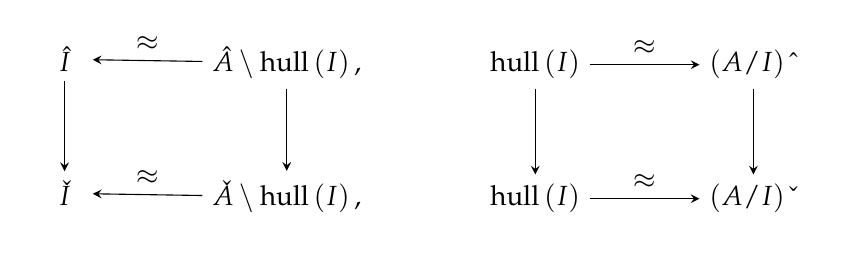
\begin{tikzpicture}
	\matrix (m) [matrix of math nodes,row sep=3em,column sep=4em,minimum width=2em]
	{
		\hat I   & \hat A\setminus \mathrm{hull}\left( I\right),  &\mathrm{hull}\left( I\right) &	\left( A/I\right)\hat~ \\ 
		\check I  &  \check A\setminus \mathrm{hull}\left( I\right), & \mathrm{hull}\left( I\right) & 	\left( A/I\right)\check~\\};
	\path[-stealth]
	(m-1-2) edge node [above] {$\approx $} (m-1-1)
	(m-1-3) edge node [above] {$\approx$} (m-1-4)
	(m-2-2) edge node [above] {$\approx$} (m-2-1)
	(m-2-3) edge node [above] {$\approx$} (m-2-4)
	(m-1-1) edge node [right]  {} (m-2-1)
	(m-1-2) edge node [right]  {} (m-2-2)
	(m-1-3) edge node [right] {} (m-2-3)
	(m-1-4) edge node [right] {} (m-2-4);
\end{tikzpicture}
\\ 	
	
\end{enumerate}

\end{theorem}
	\begin{proposition}\label{lift_prop}\cite{murphy}
		Let $B$ be a $C^*$-algebra. For each positive functional $\phi$ on $B$ there is a norm preserving extension of $\phi$ to a positive functional on $A$. If $B$ is hereditary this extension is unique.
	\end{proposition}
	\begin{proposition}\label{state_prop}\cite{pedersen:ca_aut}
		If $B$ is a $C^*$-subalgebra of $A$ then each pure state of $B$ can be extended to a pure state of $A$.
	\end{proposition}
	\begin{proposition}\label{sur_prop}\cite{pedersen:ca_aut}
		If $B$ is a $C^*$-subalgebra of $A$ then for each irreducible representation $\rho: B \to B\left( \H_1\right)$ of $B$ there is an irreducible representation $A \to B\left(\H \right)$ of $A$ with a closed subspace $\H_1 \subset \H$ such that $\rho_B  :B \to B\left(\H_1 \right)$ is spatially equivalent to $\rho: B \to B\left( \H_1\right)$.  
	\end{proposition}	
	\begin{thm}(Dauns Hofmann)\label{dauns_hofmann_thm}\cite{pedersen:ca_aut}
		For each $C^*$-algebra $A$ there is the natural isomorphism from the center of $M\left( A\right)$ onto the class of bounded continuous  functions on $\check{A}$. 
	\end{thm}
	\begin{theorem}\label{lower_norm_thm}\cite{rae:ctr_morita}
%Lemma A.30.
		Suppose that $A$ is a $C^*$-algebra and that $a \in A$.
		\begin{enumerate}
			\item [(a)] The function $x \mapsto \left\| \rep_x\left(a \right) \right\|$ is lower semi-continuous on $\hat A$; that is $$\left\{x \in \hat A~|~  \left\| \rep_x\left(a \right) \right\|\le k \right\}$$ is closed for all $k \ge 0$.
			\item[(b)] For each $k > 0$, $\left\{x \in \hat A~|~  \left\| \rep_x\left(a \right) \right\|\ge k \right\}$ is compact.
		\end{enumerate}
	\end{theorem}
\begin{definition}\label{ctr_homo_defn}\cite{fell:operator_fields} 
	A $C^*$-algebra is \textit{homogeneous of order} $n$ if every irreducible $*$-representation is of the same finite dimension $n$.
\end{definition}
\begin{remark}\label{ctr_homo_rem}\cite{fell:operator_fields} 
If $\sX$ is a spectrum of a {homogeneous of order} $n$ algebra $A$ then $A$ corresponds  some fibre bundle  with base space $\sX$,
\end{remark}
	\begin{proposition}\label{less_n_pi_prop}\cite{pedersen:ca_aut}
		%4.4.10
		The subset $_n\check{A}$ of $\check{A}$ corresponding to irreducible representations of $A$ with finite dimension less or equal to $n$ is closed. The set $_n\check{A}\setminus_{n-1}\check{A}$ of $n$-dimensional representations is a Hausdorff space in its relative topology.
	\end{proposition}

	\begin{defn}\label{spectral_proj_defn}\cite{reed_simon:mp_1}
		Let $A$ be a bounded self-adjoint operator and $\Om$ a Borel set of $\mathbb{R}$. If $\chi_\Om$ is the characteristic function of $\Om$ (cf. Definition \ref{top_characteristic_function_defn}) then $P_\Om=\chi_\Om\left(A\right)$ is called the \textit{spectral projection} of $A$.
	\end{defn}
	
	\begin{empt} \cite{rae:ctr_morita}
		Let $\hat A$ be the space of primitive ideals of $A$.
		The topology on $\hat A$ always determines the ideal structure of $A$: the open
		sets $\sU$ in $\mathrm{Prim}~ A$ are in one-to-one correspondence with the ideals
		\be\label{open_ideal_eqn}
		\left.A\right|_\sU \stackrel{\mathrm{def}}{=} \bigcap \left\{\left.P\in \hat A~\right| P \notin \sU\right\}
		\ee
		and there are natural homeomorphisms $P \mapsto P\cap \sU$ of $\sU$ onto the set of primitive ideals of  $ \left.A\right|_\sU$, and
		$P \mapsto P/A_\sU$ of $\hat A \setminus \sU$ onto  the set of primitive ideals of  $A/A_\sU$. %(Proposition A.27). 
		When $\hat A$
		is a (locally compact) Hausdorff space $T$, we can localize at a point $t$   that is,
		examine behavior in a neighbourhood of $t$   either by looking at the ideal $A_\sU$
		corresponding to an open neighbourhood $\sU$ of $t$, or by passing to the quotient
		\be\label{closed_ideal_eqn}
		\left.A\right|^F \stackrel{\text{def}}{=} A/\left( 
		\left.A\right|_{\hat A \setminus F} \right) 
		\ee
		corresponding to a compact neighbourhood $F$ of $t$. 
		%Since	life seems to be technically less complicated this way, we have chosen the $A \mapsto A^F$	option.
		%We shall need two lemmas about localization. The first is a corollary of the Dauns-Hofmann Theorem,and the second says that localizing A-B imprimitivity bimodules gives AF-F BF imprimitivity bimodules.
	\end{empt}
	\begin{remark}
		Clearly there are natural injective  $\left.A\right|_\sU \to A$ and surjective $A \hookto \left.A\right|^F$ $*$-homomorphisms,
		
	\end{remark}
	
	\begin{remark}
		The notations  \ref{open_ideal_eqn} and \ref{closed_ideal_eqn} slightly differs from  \cite{rae:ctr_morita}. Here we write $	\left.A\right|_\sU $ and $\left.A\right|^F$ instead of $\left.A\right._\sU $ and $\left.A\right.^F$ respectively.
	\end{remark}
	
	%\begin{proposition}\label{separable_polish_prop}\cite{rae:ctr_morita}% Proposition A.46. 
	%	If $A$ is a separable $C^*$-algebra, then the space $P(A)$ of pure states of $A$ is a Polish space.
	%\end{proposition}
	
	\begin{definition}\label{atomic_repr_defn}\cite{pedersen:ca_aut}
		Let $A$ be a $C^*$-algebra with the spectrum $\hat A$. We choose for any $t \in \hat A$ a pure state $\phi_t$ and  associated representation $\pi_t: A \to B\left(\H_t\right)$.
		The representation 
		\be
		\pi_a = \bigoplus_{t \in \hat A} \pi_t \quad \text{on the closure } \H_a \text{ of an algebraic direct sum}\quad  \bigoplus_{t \in \hat A} \H_t
		\ee
		is called the (reduced) \textit{atomic representation} of $A$. Any two atomic representations are unitary equivalent and any atomic representation of $A$ is faithful and nondegenerate  (cf.  Definitions \ref{faithful_representation_defn}, \ref{nondegenerate_repr_defn} and \cite{pedersen:ca_aut}).
	\end{definition}

\begin{lemma}\label{atomic_uni_lem}\cite{pedersen:ca_aut}
If  $\pi_a: A \hookto B\left( \H_a\right)$ is the atomic representation then one has
$$
\pi_a\left( A\right)'' = \prod_{x\in \hat A} B\left( \H_x\right). 
$$
\end{lemma}
\begin{theorem}\label{vn_ext_thm}\cite{pedersen:ca_aut}
%3.7.7. THEOREM. 
For each nondegenerate representation $A \to B\left(\H \right)$  of a $C^*$-algebra 
$A$ there is a unique normal morphism $\pi$ of $A''$ onto $\pi\left(A\right)''$ which extends $\pi$. 
\end{theorem}
	%\begin{definition}
	%	3.8.1. 
	%	With each (nondegenerate) representation $\pi: A \to B\left(\H\right)$ of a $C^*$-algebra $A$ we associate the projection $c\left(\pi\right)$ in the center of $A''$ for which $A''\left(\pi\right)$ is isomorphic 	to $\pi(A)''$( = $\pi''\left(A'' \right)$ ). We say that  $c\left(\pi\right)$ is the \textit{central cover  } of $\pi: A \to B\left(\H\right)$
	%\end{definition}
	%\begin{theorem}
	%		3.8.2. THEOREM. 
	%	Two representations $\pi_1: A \to B\left(\H_1\right)$ and $\pi: A \to B\left(\H_2\right)$ of a $C^*$-algebra $A$ 	are equivalent if and only if $c\left(\pi\right)= c\left(\pi\right)$, and the map $\left( \pi: A \to B\left(\H\right)\right)\mapsto c(\pi)$ gives a 	bijective correspondence between equivalence classes of representations of $A$ and 	non-zero central projections in $A''$ 
	%\end{theorem}
	
		\section{Hilbert modules and compact operators}\label{hilbert_modules_chap}
	%\paragraph{} We refer to \cite{blackadar:ko} for definition of Hilbert $C^*$-modules, or simply Hilbert modules.
	\begin{definition}\label{banach_non_defn}\cite{rae:ctr_morita}
		A left  $A$-module $X$ \textit{Banach} $A$-\textit{module} if $X$ is a Banach space and $\left\| a \cdot x\right\| \le \left\|a \right\| \left\| x\right\|$ for all $a\in A$ and $x\in\sX$.
		A  \textit{Banach} $A$-{module} is \textit{nondegenerate}  
		is nondegenerate if $\text{span}\left\{\left.a \cdot x\right|a\in A\quad x\in \sX\right\}$
		is dense in $X$. We then have \\$a_\la\cdot x \to x$
		whenever $x\in\sX$ and $\left\{a_\la\right\}$
		is a bounded approximate identity for $A$. 
	\end{definition}
	
	\begin{proposition}\label{banach_non_prop}\cite{rae:ctr_morita}
		%Proposition 2.33. 
		Suppose that $X$ 
		is a nondegenerate Banach $A$-module. Then 
		every element of $X$ 
		is of the form $a\cdot x$
		for some $a\in A$ and $x\in X$.
	\end{proposition}
	
	\begin{definition}\label{hilbert_module_defn}Paschke \cite{Paschke:73}, Rieffel \cite{Rieffel:74a}
		Let~$B$ be a $C^*$-algebra.  A \emph{pre-Hilbert $B$-module} is a right
		$B$-module~$X$ (with a compatible $\C$-vector space structure),
		equipped with a conjugate-bilinear map (linear in the second variable)
		$\left\langle{\blank},{\blank}\right\rangle_B\colon X\times X\to B$ satisfying
		\begin{enumerate}
			\item[(a)] $\left\langle{x},{x}\right\rangle_B\ge0$ for all $x\in X$;
			\item[(b)] $\left\langle{x},{x}\right\rangle_B=0$ only if $x=0$;
			\item[(c)] $\left\langle{x},{y}\right\rangle_B=\left\langle{y},{x}\right\rangle_B^\ast$ for all $x,y\in X$;
			\item[(d)] $\left\langle{x},{y\cdot a}\right\rangle_B=\left\langle{x},{y}\right\rangle_B\cdot a$ for all $x,y\in X$, $a\in B$.
		\end{enumerate}
		The map $\left\langle{\blank},{\blank}\right\rangle_B$ is called a \emph{$B$-valued inner product
			on~$X$}.
		Following equation
		\be\label{hilbert_module_norm_eqn}
		\|x\|=\|\left\langle{x},{x}\right\rangle_B\|^{\nicefrac{1}{2}}
		\ee defines a norm on~$X$.
		If~$X$ is complete with respect to this norm, it is called a $C^*$-\emph{Hilbert
			$B$-module} or simply a \emph{Hilbert
			$B$-module}.  
	\end{definition}
	\begin{definition}\label{full_hilb_defn}\cite{rae:ctr_morita}
		%Definition 2.8. 
		A Hilbert  $A$-module $X_A$  is a \textit{full} Hilbert $A$-module if the ideal 
		$$
		I\bydef \text{span}\left\{\left.\left\langle\xi, \eta \right\rangle_A\right| \xi, \eta\in X_A \right\} 
		$$
		is dense in $A$. 
	\end{definition}
	\begin{remark}\label{full_hilb_rem}
		Suppose that $A$ is a $C^*$-algebra and that $p$
		is a projection in $A$ 
		(or $M(A)$ ). Following facts are proven in the Example 2.12 of \cite{rae:ctr_morita}.
		Then $Ap \bydef \left\{\left.ap\right| a\in A\right\}$
		is a Hilbert $pAp$ module 
		with inner product 
		\be\label{full_hilb_eqn}
		\left\langle ap, bp \right\rangle_{pAp} \bydef pa^*bp
		\ee
		This Hilbert module is full. Similarly, $pA$ 
		is a Hilbert $A$-module which is full over  the ideal $\overline{ApA}\bydef \overline{\text{span}}\left\{\left.a p b\right| a,b \in A\right\}$
		generated by $p$, and $Ap$ 
		is itself a full left  Hilbert $\overline{ApA}$-module. 
	\end{remark}
	
	
	\begin{remark}\label{polarization_equality_rem}
		For any $C^*$-pre-Hilbert $X$ module, or more  precisely, for any sesquilinear form $\left\langle \cdot , \cdot \right\rangle$ the \textit{polarization equality}
		\be\label{polarization_equality_eqn}
		\begin{split}
			4 \left\langle \xi , \eta \right\rangle=\sum_{k = 0}^3i^k\left\langle \xi + i^k\eta, \xi + i^k\eta \right\rangle
		\end{split}
		\ee 
		is obviously satisfied for all $\xi, \eta \in X$.  If $\H$ is a Hilbert space then there is the following analog of the identity \eqref{polarization_equality_eqn}
		\be\label{polarization_hilb_equality_eqn}
		\\
		\left( \xi , \eta \right)_{\H} = \frac{\sum_{k = 0}^3i^k\left\| \xi + i^k\eta \right\|}{4}, \quad\forall \xi, \eta \in X
		\ee
	\end{remark}
	\begin{definition}\label{adjointable_operator_defn}\cite{matro:hcm}
		Let $X$, $Y$ be Hilbert modules over $C^*$-algebra $A$. A bounded $\C$-linear $A$-homomorphism from $X$ to $Y$ is called an \textit{operator} from $X$ to $Y$. Let $\Hom_A\left(X, Y \right)$ denote the set of all {operators} from $X$ to $Y$. If $Y = X$ then $\End_A\left(X\right)\bydef \Hom_A\left(X, X \right)$ is a Banach algebra. We say that $L\in \Hom_A\left(X, Y \right)$ 
		\textit{adjointable} if there is $L^*\in\Hom_A\left(Y, X\right)$ such that 
		$$
		\left\langle \eta, L \xi\right\rangle_A=  \left\langle L^*\eta,  \xi\right\rangle_A \quad  \forall \xi\in X,~ \eta \in Y.
		$$
		Denote by $\Hom^*_A\left(X, Y \right)\subset \Hom_A\left(X, Y \right)$ of all  {adjointable} operators. The set $\End^*_A\left(X \right)\bydef \Hom^*_A\left(X, X \right)$ is a  $C^*$-algebra.
	\end{definition}
	\begin{defn}\label{compact_a_operator_defn}\cite{pedersen:ca_aut}
		If $X$ is a $C^*$ Hilbert $A$-rigged module then
		denote by $\theta_{\xi, \zeta} \in \End^*_A\left(X \right)$   such that
		\begin{equation}\label{rank_one_eqn}
	\forall  \xi, \eta, \zeta \in X\quad		\theta_{\xi, \zeta} (\eta) = \zeta \langle\xi, \eta \rangle_X.
		\end{equation}
		The $C^*$-norm closure of  a generated by such endomorphisms ideal is said to be the {\it algebra of compact operators} which we denote by $\mathcal{K}(X)$. The $\mathcal{K}(X)$ is an ideal of  $\End^*_A(X)$.
	\end{defn}
\begin{remark}
 Also we shall use a following notation 
\be\label{rank_one_notation_eqn}
\begin{split}
	\xi\rangle \langle \zeta \stackrel{\text{def}}{=} \theta_{\xi, \zeta}: X_A \to X_A,\\
	\eta \mapsto \xi \langle\zeta, \eta \rangle_X.
\end{split}
\ee
\end{remark}
	\begin{theorem}\label{comp_mult_thm}\cite{blackadar:ko}
		Let $X_A$ is a Hilbert $A$-module.
		The $C^*$-algebra of adjointable maps  $\End^*_A\left( X_A\right)\bydef \Hom^*_A\left( X_A, X_A\right)$ is naturally isomorphic to the algebra $M\left(\K\left( X_A\right) \right)$ of multiplies of compact operators $\K\left( X_A\right)$. 
	\end{theorem}
	
	\begin{remark}
		The text of the Theorem \ref{comp_mult_thm} differs from the text of the Theorem 13.4.1 \cite{blackadar:ko}. It is made for a compatibility with this book.
	\end{remark}
	\begin{defn}\label{standard_h_m_defn}(cf. \cite{matro:hcm}) 
		The direct sum of countable  number of copies of a Hilbert module $X$ is denoted by $\ell^2\left(X \right)$. The Hilbert module  
		$\ell^2\left( A\right)$ is said to be the \textit{standard Hilbert $A$-module} over $A$. If $A$ is unital then $\ell^2\left( A\right)$ possesses the standard basis $\left\{\xi_j\right\}_{j \in \N}$.
		\begin{equation}\label{st_hilb_eqn}
			\begin{split}
				\ell^2\left( A\right) = \left\{\left\{a_n\right\}_{n \in \N}\in A^{\N}~|~\sum_{n =1}^\infty a^*_na_n < \infty \right\},\\
				\left\langle\left\{a_n\right\}, \left\{b_n\right\}\right\rangle_{\ell^2\left( A\right)}=\sum_{n =1}^\infty a^*_nb_n.
			\end{split}
		\end{equation}
	\end{defn}
	\begin{thm}\label{kasparov_stab_thm}\textbf{Kasparov Stabilization or Absorption Theorem.}\cite{blackadar:ko}
		%Theorem 13.6.2. 
		If $X_A$ is a countably generated Hilbert $A$-module, then $X_A \oplus \ell^2\left( A\right) \cong \ell^2\left( A\right)$.
	\end{thm}
	\begin{theorem}\label{fin_hpro_thm}\cite{wegge_olsen}
		%	Theorem 15.4.2
		Let $A$ be a unital C$*$-algebra. The following conditions 
		on a right $A$-module $\E$ are equivalent: 
		\begin{enumerate}
			\item [(a)] $\E$  is projective and algebraically finitely generated.
			\item [(b)] $\E$ s isomorphic as a module to a direct summand in $A^n$ for some $n\in N$. 
			\item [(c)] $\E$  is isomorphic as a module to a closed, algebraically finitely generated submodule of $\ell^2\left( A\right)$. 
			\item [(d)] $\E\cong Q\ell^2\left( A\right) $ for some compact projection $Q\in \K\left( \ell^2\left( A\right)  \right)$. 
			\item [(e)] $\E\cong Q\ell^2\left( A\right) $ for some compact projection $Q\in \K\left( \ell^2\left( A\right)  \right)$ with $Q < P_n$.
			
		\end{enumerate}
		In particular, every algebraically finitely generated projective $A$-module can 
		be endowed with a structure as a Hilbert $A$-module.
	\end{theorem}
	\begin{corollary}\label{fin_hpro_cor}\cite{wegge_olsen}
		%Corollary 15.4.8. 
		Any algebraically finitely generated Hilbert module over 
		a unital $C^*$-algebra is projective. 
	\end{corollary}
	
	\begin{remark}\label{fin_gen_un_equ_rem}\cite{wegge_olsen}
		If $A$ is an unital $C^*$-algebra and $X_A$ is a Hilbert $A$-module then the following conditions are equivalent
		\begin{itemize}
			\item [(a)] $X_A$ is algebraically finitely generated.
			\item[(b)]  The $C^*$-algebra $\K\left(X_A \right)$ of compact operators is unital. (cf. \cite{wegge_olsen} Remark 15.4.3).
		\end{itemize}
	\end{remark}
	\begin{definition}\label{c_misch_defn}\cite{sol_tro:ca_op}
		Let $A$ be an unital $C^*$-algebra a bounded $A$ operator $K: \ell^2\left( A\right) \to \ell^2\left( A\right)$ is \textit{compact} (in the sense of Mishchenko) if we have 
		$$
		\lim_{n \to \infty}\left\|\left.K\right|_{L_n^\perp} \right\| = 0,
		$$
		where $L_n = \oplus_{j=1}^n A \subset \ell^2\left( A\right)= \oplus_{j=1}^\infty A$,  $L^\perp_n = \oplus_{j=n+1}^\infty A \subset \ell^2\left( A\right)= \oplus_{j=1}^\infty A$.
	\end{definition}
	\begin{remark}\label{c_misch_rem}\cite{sol_tro:ca_op}
		If $C^*$-algebra $A$  is unital then
		any {compact} (in the sense of Mishchenko) operator is compact in the sense of the Definition \ref{compact_a_operator_defn}, and vice versa.
	\end{remark}
	
	
	\begin{lemma}\label{c_misch_lem}\cite{sol_tro:ca_op}
		Let $K: \ell^2\left( A\right) \to \ell^2\left( A\right)$ be \textit{compact} operator (in the sense of Mishchenko).
		Let $p_n$ be the projection on $L_n$ along $L^\perp_n$. The following properties are equivalent.
		\begin{enumerate}
			\item [(i)] $\lim_{n \to \infty}\left\|\left.K\right|_{L_n^\perp} \right\| = 0$.
			\item[(ii)] $\lim_{n \to \infty}\left\|Kp_n - K \right\| = 0$.
			\item[(iii)] $\lim_{n \to \infty}\left\|p_n K - K \right\| = 0$.
		\end{enumerate} 
		
	\end{lemma}
	
	
	\begin{empt}\label{hm_dual_empt}\cite{matro:hcm}
		For a Hilbert $C^*$-module $X$ over $C^*$-algebra $A$ let us denote by $X'$ the set of  all bounded $A$-linear maps  from  $X$ to $A$. 
		The formula
		\be
		\left( f \cdot a\right)\left( \xi\right) \bydef a^*f\left( x\right); \quad a \in A, \quad f \in X' , \quad \xi \in X
		\ee
		introduced the structure if right $A$-module on $X'$.
		The elements of $X'$ are called \textit{functionals} on a Hilbert module $X$. Note that there is an obvious isometric inclusion
		\be\label{to_dual_eqn}
		\begin{split}
			X \subset X',\\
			x \mapsto\left\langle x, \cdot \right\rangle.
		\end{split}
		\ee
		The space $X'$ is called the \textit{dual Banach module} of $X$.
	\end{empt}	
	\begin{definition}\label{hm_selfdual_defn}\cite{matro:hcm}
		A Hilbert module $X$ is called  \textit{self-dual} if $X\cong X'$.
	\end{definition}
	\begin{definition}\label{hm_MI_defn}\cite{matro:hcm}
		A $C^*$-algebra is said to be \textit{module}-\textit{infinite} (MI) if each countably generated Hilbert $A$-module is projective and finitely generated if and only if it is self-dual.
	\end{definition}
	
	\begin{definition}\label{hm_di_empt}\cite{matro:hcm}
		A commutative $C^*$-algebra $A = C\left(\sY \right)$ is said to be DI (\textit{divisible infinite}) if for any infinite sequence $\left\{u_j\right\}_{j\in \N}$ of norm $1\ge\left\|u_j \right|\ge C > 0$ in $A$ there exists a subsequence $j\left(k\right)$ and elements $0 < b_k \in A$ of norm 1 such that
		\begin{enumerate}
			\item [(i)] The supports $b_k$ in $\sY$ are pairwise disjoint.
			\item[(ii)] For each $k$ there exists points $y_k, ~y'_k$ such that $b_k\left(y_k\right)= 1$, $y'_k \notin \supp b_k$, $~\left\|u_{j\left(y_k\right)} \right|\ge\delta$, $~\left\|u_{j\left(y'_k\right)} \right|\ge\delta$ and the sequences $\left\{y_k\right\}, ~ \left\{y'_k\right\}$ have a common accumulation point. In particular $\sum_k b_k^s$ is a discontinuous function for any integer $s\ge 1$.
		\end{enumerate} 
	\end{definition}
	\begin{theorem}\label{hm_di_mi_thm}\cite{matro:hcm}
		If a commutative unital $C^*$-algebra $A$ is $\mathrm{DI}$, then it is  $\mathrm{MI}$.
	\end{theorem}
	
	\begin{theorem}\label{hm_sep_di_thm}\cite{matro:hcm}
		A commutative separable  unital $C^*$-algebra $A$ is $\mathrm{DI}$ if and only if its Gelfand spectrum has no isolated points.
	\end{theorem}	
	%\begin{empt}\cite{matro:hcm}
	%	For a Hilbert $C^*$-module $X$ over $C^*$-algebra $A$ we define the \textit{bidual} Banach right $A$ module $X''$ as a set of all bounded $A$-homomorphism from the dual module $X'$ into $A$. 
	%\end{empt}	
	
	%\begin{definition}\label{hm_reflexive_defn}\cite{matro:hcm}
	%A Hilbert $C^*$-module $X$ is called  \textit{reflexive} if $X''\cong X$.
	%\end{definition}
	\section{Regular operators}
	\paragraph{}
	Here I follow to \cite{Vassout:Unbounded_groupoids}.
	Unlike the case of Hilbert spaces (when $A = \C$), a closed submodule $F$ of a Hilbert module $F$ 
	does not have an orthogonal complement $F^\perp$ such that $F \oplus F^\perp = E$. If this is nevertheless the
	case, we say that $F$ is {\it orthocomplemented} in $F$.
	$A$ {\it morphism} between two Hilbert modules $E, E'$
	on $A$ is an $A$-linear operator admitting an
	adjoint (for the involved $A$-valued scalar products). Morphisms from $E$ to $E'$
	 are bounded and we
	denote the space of morphisms by $\L\left(E, E' \right)$ . A bounded $A$-linear map $T: E \to E'$
	 is a morphism
	if and only if the graph of $T$ is orthocomplemented in $E\oplus E'$
% We will use the following easy fact from
\begin{proposition} Let $T \in \L\left(E, E' \right)$. 
\begin{enumerate}
	\item [(i)]
	\begin{enumerate}
		\item [(a)]  If $T$ is surjective then $TT^*$ is invertible in $\L\left( E'\right)$
	 and $E = \ker T \oplus \im T^*er T ?Im T$;
	\item [(b)] 
		If $T$ is bijective, then so is $T^*$. We have $T^{-1}\in \L\left(E', E \right)$  and $\left( T^{-1}\right)^* = \left( T^*\right)^{-1}$,
		
	\end{enumerate}
		\item [(ii)] The following conditions are equivalent:
	\begin{enumerate}
	\item[(a)]	$\in T$ is closed in $E'$;
	\item[(b)]	$\in T^*$ is closed in $E$;
\item[(c)] $0$ is isolated in the spectrum of $T^*T$,

	If these conditions are satisfied, then $\im T$ and $\im T^*$
 are orthocomplemented submodules
	of $E'$ and $E$
	with $\im T \oplus \ker T^* = E$ and  $\im T^* \oplus \ker T = E$.
	\end{enumerate}
	
\end{enumerate}
\end{proposition}
\begin{definition}
An unbounded operator $T : E \to E'$
 is defined by its graph $G\left(T \right) \bydef \left\{\left(x, Tx \right) .| x \in \dom T\right\}$ 
which is a sub-$A$-module of $E \oplus E$
 If $\left(\dom T \right)^\perp= 0$, then there is a natural definition for $T^*$
by its graph. A densely defined operator $T$ , with densely defined adjoint is said to be {\it regular} if
its graph $G\left( T\right)$ is orthocomplemented. This is the case if and only if $1 + T^*T$ is surjective and
then $\left( 1 + T^*T\right)^{-1}$  is a morphism. Taking the square root we have that $\left( 1 + T^*T\right)^{-\nicefrac{1}{2}}$ is of image
$\dom T$ and such that $Q\left( T\right)\bydef \left( 1 + T^*T\right)^{-2}$  is a morphism.
\end{definition}
The map $T \mapsto Q(T)$ is a 1�1 correspondence between regular operators and morphisms $Q$
with norm less than one and such that $\im \left(1 - Q^*Q \right)$  is dense in $E$, called the Woronowicz
transform. A regular operator $T$ is {\it self-adjoint} if $T^*=T$ , respectively {\it normal} if $T^*T = TT^{*}$.
This is the case if and only if $Q(T )$ is self-adjoint, respectively normal.


The {\it resolvent} $R_\la(T ) = (T ? \la)^{-1}$,
of a regular operator $T$ is an analytic map from $\C-\mathrm{Sp} T$
to $\L\left( E\right)$  and a regular operator $T$ (with spectrum = C) is normal if and only if $R_\la\left( T\right)$  is. The
natural correspondence between regular operators and morphisms allows to define a continuous
functional calculus for normal regular operators.
\begin{theorem}
Let $T$ be a regular normal operator on a Hilbert module $E$ and $X$ be a closed set
in $\C$ with $\mathrm{Sp} T \subset X$. Then any map $f \in C(X)$ defines a normal regular operator $f (T )$, with $\left(f \left( T\right) \right)= \overline f\left( T^*\right)$ such that:	
		\begin{enumerate}
\item [{{(1)}}] For any pair $(f, g)$ of continuous functions, $(f + g)(T )$ is the closure of $f (T ) + g(T )$ and
$(fg)(T )$ the closure of $f (T )g(T )$.
\item [{(2)}] If $f$ is continuous and bounded, we have $f\left( T\right)\in \L\left(E \right)$   and $\left\| f (T ) \right\| = \sup_{\la \in \mathrm{Sp} T } \left\| f (\la ) \right\|$, 
\item [{(3)}] $\mathrm{Sp} f(T)$ is the closure in $\C$ of $f\left(\mathrm{Sp} T \right)$.
\item [{(4)}] For $f, g \in C\left( C\right)$ , we have $(f \circ g)(T ) = f (g(T ))$.
\item [{(5)}] $\Id_X\left( T\right) = T$ and $q(T ) = Q(T )$ if q is the map $q(z) = z/(1 + |z|^2)$.
\item [{(6)}] If $T\in \L(E)$, the map $f \mapsto f\left( T\right)$  coincides with the continuous functional calculus in the
$C^*$-algebra $\L(E)$.		
	\end{enumerate}

		
\end{theorem}
Now let $E$ be a Hilbert module on a $C^*$-algebra $A$ and $\pi: A\to \L\left( H\right)$  a representation of $A$
on a Hilbert module $H$ on a $C^*$-algebra $B$. A morphism $T \in \L(E)$ can be pushed forward to a morphism $T \otimes_\pi  1 \in \L\left(E \otimes_\pi H \right)$ . This extends to regular operators.
\begin{proposition}
%Proposition 4. 
Let $T$ be a regular operator on $E$ and $\pi A\to \L\left(H \right)$  a representation of $A$ on a
$B$-Hilbert module $H$. Then $T\otimes_\pi !$ is a regular operator on the $B$-Hilbert module $E\otimes_\pi H$ and
we have:
		\begin{enumerate}
	\item [{{(1)}}] $Q\left(T\otimes_\pi 1 \right) = Q\left(T \right) \otimes_\pi 1$ and  $\left(T^*\otimes_\pi 1 \right) = T^* \otimes_\pi$ and  $\left(T^*\otimes_\pi 1 \right)\left(T\otimes_\pi 1 \right)= T^*T\otimes_\pi 1 $.
	\item [{(2)}] If $T$ is normal or self-adjoint, then so is $T \otimes_\pi 1$.
	\item [{(4)}] If $D \in \dom T$ is a core for $T$ , and $\H$ a dense subspace in $H$, then $D\otimes_{alg} H$ is a core for
	$T \otimes_\pi 1$..
	\item [{(5)}] We have $\mathrm{Sp}\left(T \otimes_\pi  1\right) \subset \mathrm{Sp} T$ with equality when $\pi$ is injective..
	\item [{(6)}] If $T$ is normal and $f \in \C(X)$ with $X$ closed and $\mathrm{Sp} T \subset X$ then $f \left(T\otimes_\pi 1 \right) = f\left( T\right) \otimes_\pi 1$,		
\end{enumerate}

\end{proposition}

	\section{Hermitian  modules and functors}
	\paragraph*{}
	In this section we consider an analogue of the $A \otimes_B - : \ _B\mathcal{M}\to _A\mathcal{M}$ functor or an algebraic generalization of continuous maps. Following text is in fact a citation of \cite{rieffel_morita}.
	
	\begin{defn}\label{herm_mod_defn}
		\cite{rieffel_morita} Let $B$ be a $C^*$-algebra. By a (left) {\it Hermitian  $B$-module} we will mean the Hilbert space $\H$ of a nondegenerate $*$-representation $A \rightarrow B(\H)$. Denote by $\mathbf{Herm}(B)$ the category of Hermitian  $B$-modules.
	\end{defn}
	\begin{empt}
		\cite{rieffel_morita} Let $A$, $B$ be $C^*$-algebras. In this section we will study some general methods for construction of functors from  $\mathbf{Herm}(B)$ to  $\mathbf{Herm}(A)$.
	\end{empt}
	
	
	\begin{defn}\label{corr_defn}\cite{rieffel_morita}
		Let $A$ and $B$ be $C^*$-algebras. By a {\it Hermitian  $B$-rigged $A$-module} we mean a $C^*$-Hilbert $B$ module, which is a left  $A$-module by means of $*$-homomorphism of $A$ into $\mathcal{L}_B(X)$.
	\end{defn}
	
	\begin{empt}\label{herm_functor_empt}
		Let $X$ be a Hermitian $B$-rigged $A$-module. If $V\in \mathbf{Herm}(B)$ then we can form the algebraic tensor product $X \otimes_{B_{\mathrm{alg}}} V$, and equip it with an ordinary pre-inner-product which is defined on elementary tensors by
		\begin{equation}\label{inital_hilb_prod_eqn}
			\langle x \otimes v, x' \otimes v' \rangle = \langle \langle x',x \rangle_B v, v' \rangle_V.
		\end{equation}
		Completing the quotient $X \otimes_{B_{\mathrm{alg}}} V$ by subspace of vectors of length zero, we obtain an ordinary Hilbert space, on which $A$ acts by 
		\be\label{comp_hilb_act_eqn}
		a(x \otimes v)=ax\otimes v
		\ee to give a  $*$-representation of $A$. We will denote the corresponding Hermitian  module by $X \otimes_{B} V$. The above construction defines a functor $X \otimes_{B} -: \mathbf{Herm}(B)\to \mathbf{Herm}(A)$ if for $V,W \in \mathbf{Herm}(B)$ and $f\in \mathrm{Hom}_B(V,W)$ we define $f\otimes X \in \mathrm{Hom}_A(V\otimes X, W\otimes X)$ on elementary tensors by $(f \otimes X)(x \otimes v)=x \otimes f(v)$.	We can define action of $B$ on $V\otimes X$ which is defined on elementary tensors by
		\begin{equation}\nonumber\label{comp_hilb_pre_act_eqn}
			b(x \otimes v)= (x \otimes bv) = x b \otimes v.
		\end{equation}
		The complete proof of above facts is contained in the Proposition 2.66 \cite{rae:ctr_morita}
	\end{empt}
	\begin{defn}\label{induced_representation_defn}\cite{rae:ctr_morita}
		Let us consider the situation \ref{herm_functor_empt}. 	The functor $X \otimes_{B} -: \mathbf{Herm}(B)\to \mathbf{Herm}(A)$ is said to be the \textit{Rieffel correspondence}. If $\pi: B \to B\left( \H_B\right)$ a representation then the representation $\rho :  A \to B\left( \H_A\right)$  given by the functor $X \otimes_{B} -: \mathbf{Herm}(B)\to \mathbf{Herm}(A)$ is said to be the \textit{induced representation}. We use following notation
		\be\label{induced_representation_eqn}
		X\text{-}\Ind^A_B\pi\bydef \rho\quad \text{ or } \quad \Ind^A_B\pi\bydef \rho\quad \text{ or } \quad	 X\text{-}\Ind\pi\bydef\rho
		\ee
		(cf. Proposition 2.66 of \cite{rae:ctr_morita}).
	\end{defn}
%\begin{proposition}\label{induced_nondegenerate_prop}\cite{rae:ctr_morita}
%Proposition 2.66.
%Suppose $A$ acts as adjointable operators on a Hilbert $B$-module $X$, and $\pi$ is a nondegenerate representation of $B$ on $\H_\pi$. Then the formula
%\be\label{induced_nondegenerate_eqn}
%\Ind \pi(a)(x\ox_B h) \bydef (a \cdot x)\ox_B h
%\ee
%extends to give a representation $\Ind \pi$ of $A$ as bounded operators on the Hilbert space$X \widehat\otimes_B \H_\pi$ obtained by completing of an algebraic tensor  $X \otimes_B \H_\pi$ in the inner product satisfying \eqref{inital_hilb_prod_eqn}. If $X$ is nondegenerate as an $A$-module (i.e., if $A\cdot X$ is dense in $X$), then $\Ind \pi$ is a nondegenerate representation of $A$ on $X \widehat\otimes_B \H_\pi$.
%\end{proposition}
	
	\begin{remark}\label{left_right_rem}
		If $A$ is a $C^*$-algebra and $A \to B\left(\H \right)$ is a representation then $\left(a \xi, \eta \right)_{\H}  = \left( \xi, a^* \eta \right)_{\H}$ for each $a \in A$ and $\xi, \eta$. Taking into account (c) of the Definition \ref{hilbert_module_defn}  the equation \eqref{inital_hilb_prod_eqn} can be rewritten by following way
		
		\begin{equation}\label{hilb_prod_eqn}
			\langle x \otimes v, x' \otimes v' \rangle = \langle v,  \langle x,x '\rangle_B v' \rangle_V.
		\end{equation}
		The equation \eqref{hilb_prod_eqn} is more convenient for our purposes than \eqref{inital_hilb_prod_eqn} one. %Similarly the equation \eqref{comp_hilb_pre_act_eqn}is replaced with
		
	\end{remark}
	
	
	\section{$C^*$-correspondences}\label{correspondeces_chap}
Here I follow to \cite{uni_groupoid_ca}.
	A $C^*$-\textit{correspondence} from a $C^*$-algebra~$A$
	to another $C^*$-algebra~$D$
	consists of a (right) Hilbert $D$-module~$\F$
	with a nondegenerate $*$-homomorphism~\(\varphi\) from~$A$
	to~$\mathbb{B}(\F)$,
	the $C^*$-algebra of adjointable operators on~$\F$.
	We view a $C^*$-correspondence from~$A$
	to~$D$
	as an arrow \(A\to D\)
	and usually write $A\xrightarrow{\F} D$.
	We also view~\(\varphi\)
	as a \emph{representation} of~$A$
	on~$\F$.
	Two $C^*$-correspondences
	$\F_1$)
	and~$\F_2$)
	from~$A$
	to~$D$
	are \emph{isomorphic} if there is a unitary bimodule map
	$U: \F_1 \xrightarrow{\sim} \F_2$.
	
	We write~\(\otimes\)
	for suitably completed tensor products of $C^*$-correspondences,
	and~\(\odot\)
	for the tensor product of vector spaces without any completion.
	In particular, the composite of two $C^*$-correspondences
	$A\xrightarrow{\E} B$ and $B\xrightarrow{\F} D$ is their
	(balanced) tensor product~$\E \ox_B \F$
	(see~\cite{Lance:Hilbert_modules}%*{Chapter~4}
	). This is
	the completion of the algebraic (balanced) tensor product
	~$\E \odot_B \F$) with respect to the $D$-valued inner product
	$$
\left\langle \xi_1\ox \eta_1, \xi_2\ox \eta_1 \right\rangle\bydef  \left\langle \eta_1, \varphi\left(\xi_1, \xi_2 \right) \right\rangle 
$$
	where $\varphi\colon B\to \mathbb{B}\left(\F \right)$  is the underlying
	homomorphism that gives the left  $B$-module structure of~$\F$;
	the notation $\E \ox_\varphi \F$ is used instead of
$\E \ox_B \F$ to highlight~$\varphi$.
	
	
	\section{Strong Morita equivalence for $C^*$-algebras}\label{strong_morita_sec}

	\paragraph*{}
	The notion of the strong Morita
	equivalence was introduced by Rieffel.
	\begin{definition}\label{strong_morita_defn}[Rieffel \cite{Rieffel:74a,rieffel_morita,Rieffel:76}]
		Let $A$ and~$B$ be $C^*$-algebras.  By an \emph{$A$-$B$-equivalence
			bimodule} (or \emph{$A$-$B$-imprimitivity
			bimodule}) we mean an $\left(B,A\right)$-bimodule which is equipped with $A$- and
		$B$-valued inner products with respect to which~$X$ is a right Hilbert
		$A$-module and a left  Hilbert $B$-module such that
		\begin{enumerate}
			\item[(a)] $\left\langle{x},{y}\right\rangle_B z = x\left\langle{y},{z}\right\rangle_A$ for all $x,y,z\in X$;
			\item[(b)] $\left\langle{X},{X}\right\rangle_A$ spans a dense subset of~$A$ and $\left\langle{X},{X}\right\rangle_B$ spans a dense
			subset of~$B$, i.e. $X$ is a full Hilbert $A$-module and a full Hilbert $B$-module.
		\end{enumerate}
		We call $A$ and~$B$ \emph{strongly Morita equivalent} if there is an
		$A$-$B$-equivalence bimodule.
	\end{definition}
	
	\begin{example}\label{imp_p_exm}\cite{rae:ctr_morita}
		%Example 3.6.
		Let $p$ be a projection in $M 
		(A)$. We saw in the Remark \ref{full_hilb_rem} that $Ap$
		is a full right Hilbert $pAp$-module and a full left  Hilbert $\overline{ApA}$-module. (Recall that 
		$\overline{ApA}$
		denotes the ideal generated by $p$, which is the closed span of the set $ApA$.) 
		%The 	actions and inner products are the restrictions of those in the previous example, so 	all the algebraic properties are trivially true, and 
		Thus $Ap$ is an $\overline{ApA}$-$pAp$-imprimitivity 
		bimodule. 
	\end{example}
	
	\begin{rem}
			If~$_AX_B$ be an $A$-$B$ imprimitivity bimodule then there is a \textit{dual} $B$-$A$ bimodule $_B\widetilde X_A$ which is a $B$ $A$-imprimitivity bimodule (cf. \cite{rae:ctr_morita}).
	\end{rem}
	\begin{theorem}\label{morita_herm_thm} \cite{rae:ctr_morita,Rieffel:74a}
		Let~$X$ be an $A$-$B$ equivalence bimodule.  Then given by \ref{induced_representation_defn} functor $X\otimes_B\blank$
		induces an equivalence (cf. Definition \ref{category_equivalence_definition}) between the category of Hermitian  $B$ modules and
		the category of Hermitian  $A$-modules, the inverse being given by
		$\tilde{X} \otimes_A\blank$.
		
		% This functor preserves weak containment and 	direct integrals.
	\end{theorem}
	\begin{theorem}\label{rieffel_equiv_thm}\cite{rae:ctr_morita}
		%Theorem 3.29. 
		Suppose that $X$ is an $A$ $B$-imprimitivity bimodule, and $\pi$, $\rho$
		are nondegenerate representations of $B$ 
		and $A$, respectively. Then $\widetilde X-\Ind\left(  X-\Ind \pi \right)$ is 
		naturally unitarily equivalent to $\pi$, and $X-\Ind\left(\widetilde  X-\Ind \rho \right)$ is 
		naturally unitarily equivalent to $\rho$.
		
	\end{theorem}
	\begin{corollary}\cite{rae:ctr_morita}
		%Corollary 3.312.
		If $X$ is an $A$ $B$-imprimitivity bimodule, then the inverse of the Rieffel correspondence $X-\Ind$ is  $\widetilde X-\Ind$.
	\end{corollary}
	\begin{corollary}\label{morita_irred}\cite{rae:ctr_morita}
		%Corollary 3.32. 
		Suppose that $X$ is an $A$ $B$-imprimitivity bimodule, and that $\pi$
		is 
		a nondegenerate representation of $B$. Then $\widetilde  X-\Ind \pi$
		is irreducible if and only if $\pi$ 
		is irreducible. 
	\end{corollary}
	\begin{corollary}\label{rieffel_homeo_cor}\cite{rae:ctr_morita}
		%Corollary 3.32. NOT FULL
		If $X$ is $A$-$B$-imprimitivity bimodule then the Rieffel correspondence restricts to a homeomorphism $h_X: \mathrm{Prim}~B \xrightarrow{\approx}\mathrm{Prim}~A$.
	\end{corollary}
	\begin{definition}\label{rieffel_homeo_defn}\cite{rae:ctr_morita}
		Under the hypotheses of the Corollary \ref{rieffel_homeo_cor} the homeomorphism $h_X: \mathrm{Prim}~B \xrightarrow{\approx}\mathrm{Prim}~A$
		is said to be the \textit{Rieffel homeomorphism}.
	\end{definition}
\begin{definition}\label{stable_ca_defn}\cite{wegge_olsen}
 A $C^*$-algebra A is said to be \textit{stable} when $A\otimes \K \cong  A$. %\cite{blackadar:ko}
 %Definition 1.10.1. 
The \textit{stabilization} of $A$ is $A^s\bydef A\otimes \K$. 
$C^*$-algebras $A$ and $B$ are said to be \textit{stably equivalent} when $A\otimes \K\cong B\otimes \K$.
%Definition 5.1.1.$\mathbb{M}_\infty\left(A \right)$ is the algebraic direct limit of $\mathbb{M}_n\left(A \right)$ under theembeddings $a \mapsto \text{diag}\left(a, 0\right)$.$M (A) may be thought of as the algebra of all infinite matrices over A with7only finitely many nonzero entries. Whenever it is convenient, we will identifyMn(A) with its image in the upper left-hand corner of Mn+k(A) or M (A).When it is necessary to topologize M (A), any topology inducing the naturaltopologies on Mn(A) will do. For example, M (A) may be given the inductivelimit topology if desired. Better yet, one may choose the norms on Mn(A) sothat the embeddings are isometries; M (A) is a local Banach algebra with theinduced norm.
%If $A$ is a (local) $C^*$-algebra, the embedding are isometries, so $\mathbb{M}_\infty\left(A \right)$ has anatural norm. The completion is called the \textit{stable algebra} of A, denoted $A\otimes \K$ (it is the $C^*$-tensor product of $A$ and $\K$).
\end{definition}
	\begin{theorem}\label{stable_morita_thm}\cite{brown:stable}
		%	THEOREM 1.2. 
		Let $B$ and $E$ be $C^*$-algebras. If $B$ and $E$ are 
		stably isomorphic, then they are strongly Morita equivalent. Conversely, 
		if $B$ and $E$ are strongly Morita equivalent and if they both 
		possess strictly positive elements, then they are stably isomorphic (i.e they are stably equivalent).	
	\end{theorem}
	
		\begin{proposition}\label{top_admits_morita_prop}\cite{connes:ncg94}
		%	Proposition 1. [473]  P 117 
		Let a group $\Ga$  act freely and properly on a topological space  $\widetilde \sX$ and let $\sX\bydef \widetilde \sX/\Ga$. Then
		the $C^*$-algebra $C_0\left(\sX \right)$  is strongly Morita equivalent to the  product $C^*$-algebra
		$C_0\left(\widetilde \sX\right)\rtimes \Ga$.
	\end{proposition}
	\begin{remark}\label{top_admits_morita_rem}\cite{connes:ncg94}
The equivalence
	$C^*$-bimodule $E$ is easy to describe; it is given by the bundle of Hilbert spaces $\left\{\H_x\right\}_{x\in \sX}$
 with base  $\sX$  whose fiber at $x\in\sX$ is the $\ell^2$-space of the orbit $x\in\sX$. This yields
	the required $\left(C_0\left(\widetilde \sX \right)\rtimes \Ga, C_0\left(\sX \right) \right)$  $C^*$-bimodule.
	\end{remark}

	
	
	% REPLACE WITH rieffel_homeo_cor and CHECK 
	%\begin{remark}\label{rieffel_homeo_rem}
	%	From the Theorem \ref{morita_herm_thm} it turns out that any $A$-$B$-equivalence bimodule $h_X$ induces a bijective map $\hat B \xrightarrow{\approx} \hat A$. Indeed $h_X$ is a homeomorphism (cf. Section 5.1 \cite{rae:ctr_morita}).
	%\end{remark}
	
	%\begin{proposition}\label{morita_k_prop}\cite{rae:ctr_morita}% 	Proposition 3.8. 
	%	Every full Hilbert $B$-module $X_B$ is a $\K\left(X \right)-B$-imprimitivity bi-	module with $\left\langle x,y \right\rangle_{\K\left(X\right)} \stackrel{\mathrm{def}}{=}\Th{x,y}= y\left\rangle \right\langle x $  Conversely, if $X$ is an $A$-$B$-imprimitivity bimodule, then there is an isomorphism $\phi$ of $A$ onto $\K\left(X\right)$ such that $\phi\left(\left\langle x, y \right\rangle_A\right)=  \left\langle x,y \right\rangle_{\K\left(X\right)}$ for all $x, y\in \K\left(X\right)$
	%\end{proposition}

\section{$C^*$-algebras of type I}
\subsection{Basic facts}
\paragraph*{}   Let $A$ be a $C^*$-algebra. For each positive $x\in A_+$ and irreducible representation $\pi: A \to B\left( \H\right)$   the (canonical) trace of $\pi(x)$ depends only on the equivalence class of $\pi$, so that we may define a function 
\be\label{ctr_hat_eqn}
\begin{split}
	\hat x : \hat A \to [0,\infty];\\
	\hat x\left(t \right) =\tr\left( \pi\left(x \right) \right) 
\end{split}
\ee
where $\hat A$ is the spectrum of $A$ (the space of equivalence classes of irreducible representations) and $\tr$ is the trace of the operator. From the Proposition 4.4.9 \cite{pedersen:ca_aut} it follows that $\hat x$ is lower semi-continuous function  in the Jacobson topology (cf. Definition \ref{jtop_defn}).



\begin{lemma}\label{ctr_para_sum}\cite{rae:ctr_morita}
	%Lemma 5.4. 
	Let $A$ be a $C^*$-algebra whose spectrum $\sX$ is paracompact (and hence Hausdorff). Suppose that $\left\{\sU_\a\right\}_{\a\in\mathscr A}$ is a locally finite cover   of $\sX = \cup_{\a\in\mathscr A} \sU_\a$ by relatively 
	compact open sets, $\left\{\phi_\a\right\}$
	is a partition of unity subordinate to $\left\{\sU_\a\right\}$, and $\left\{a_\a\right\}$ is a set of elements in $A$ parameterized by $\mathscr A$. If there is a function $f\in C_0\left(\sX\right)$ such 
	that $\left\| \rep_{ x}\left(a_\a \right) \right\| \le f\left( x\right)$ for all $x$ and $\a$, then there is a unique element $a$ of $A$ such that 
	$\rep_{ x}\left(a \right)= \sum_{ {\a}\in {\mathscr A}}\phi_\a \rep_{ x}\left(a_\a \right)$
	for every $x\in\sX$
	; we write $a =\sum_{ {\a}\in {\mathscr A}}\phi_\a a_\a$.
\end{lemma}
\begin{defn}\label{continuous_trace_c_a_defn}\cite{pedersen:ca_aut} We say that element $x\in A_+$ has {\it continuous trace } if $\hat x \in C_b(\hat A)$. We say that $C^*$-algebra has {\it continuous trace } if a set of elements with continuous trace  is dense in $A_+$.
\end{defn}
\begin{remark}
	If a $C^*$-algebra $A$ has {continuous trace } then for simplicity we say that $A$ is \textit{continuous-trace} $C^*$-\textit{algebra},
\end{remark}
There are alternative equivalent definitions {continuous-trace} $C^*$-{algebras}. One of them is presented below.
\begin{definition}\label{continuous_trace_c_alt_defn}\cite{rae:ctr_morita}
	%Definition 5.13. 
	A \textit{continuous-trace} $C^*$-\textit{algebra} is a $C^*$-algebra $A$ with Hausdorff
	spectrum $\sX$ such that, for each $x_0\in\sX$ there are a neighbourhood $\sU$ of $x_0$ and $a\in A$ such that $\rep_{ x}\left( a\right) $ is a rank-one projection for all $x \in \sU$.
\end{definition}
\begin{definition}\label{abelian_element_defn}\cite{pedersen:ca_aut}
	A positive element in $C^*$ - algebra $A$ is {\it Abelian} if subalgebra $xAx \subset A$ is commutative.
\end{definition}
\begin{definition}\label{type_I_defn}\cite{pedersen:ca_aut}
	We say that a $C^*$-algebra $A$ is \textit{of type} $I$ if each non-zero quotient of $A$ contains a non-zero
	Abelian element. If $A$ is even generated (as $C^*$-algebra) by its Abelian elements we say
	that it is \textit{of type} $I_0$.
\end{definition}
\begin{lemma}\label{typeI_lem}\cite{pedersen:ca_aut}
	%6.1.4	
	If $A$ is a $C^*$-algebra of operators acting irreducibly on a Hilbert space $\H$ such that $A\cap \K\left( \H\right) \neq \{0\}$ then $\K\left( \H\right)\subset A$ and each faithful representation is unitary equivalent with the identity representation.
\end{lemma}

\begin{prop}\label{abelian_element_proposition}\cite{pedersen:ca_aut}
	A positive element $x$ in $C^*$-algebra $A$ is Abelian if $\mathrm{dim}~\pi(x) \le 1$ for every irreducible representation $\pi:A \to B(\H)$.
\end{prop}
\begin{proposition}\label{ctr_pedersen_prop}\cite{pedersen:ca_aut}
%6.1.12. PROPOSITION. //
If $A$ is a $C^*$-algebra with continuous trace  there is for 
each $x$ in $K(A)_+$ an $n < \infty$ such that $\dim \pi\left(x \right)< n$  for every irreducible 
representation $\pi: A \to B\left(\H \right)$ . Moreover , the map $x \mapsto \left( \pi \mapsto \tr \circ \pi\left( x\right) \right)$  is a faithful, positive linear 
surjection of $K\left(A \right)$ onto  $K\left(\hat A \right)$. 
\end{proposition}

%Theorem 5.6
\begin{defn}\label{ccr_defn}\cite{pedersen:ca_aut}
	A $C^*$-algebra is called \textit{liminaly} (or $CCR$) if $\rho\left( A\right)= \K$ for each irreducible representation $\rho: A \to B\left( \H\right)$.  
\end{defn}

\begin{theorem}\label{ctr_hat_check_thm}\cite{pedersen:ca_aut}
	% 6.6.5
	Let $A$ be a $C^*$-algebra of type I. Then 
	\begin{enumerate}
		\item [(i)] $\K \subset \pi\left(A \right)$ for each irreducible representation $\pi: A \to B\left(\H \right)$  of $A$.
		\item[(ii)] $\hat A = \check{A}$ (cf. Definition \ref{spectrum_prime_primtive_defn}).
	\end{enumerate}
\end{theorem}
\begin{prop}\label{ctr_hered_prop}\cite{pedersen:ca_aut}
	% 6.2.10. PROPOSITION. 
	Each hereditary $C^*$-subalgebra and each quotient of a 
	$C^*$-algebra which is of type $I_0$ or has continuous trace  is of type $I_0$  or has 
	continuous trace , respectively. 
\end{prop}

\begin{corollary}\label{ctr_ccr_i_cor}\cite{pedersen:ca_aut}
	Any $CCR$ $C^*$-algebra is of type I.
\end{corollary}
\begin{definition}\label{oa_haus_defn}\cite{rae:ctr_morita}
	A topological space is called \textit{almost Hausdorff} if every closed subset
	has a dense open subset which is Hausdorff in the relative topology.
\end{definition}

\begin{theorem}\label{oa_haus_prim_thm}\cite{rae:ctr_morita}
	%	Theorem A.50. 
	Suppose that $A$ 
	is a $C^*$-algebra such that $\check{A}$
	is either second-countable  or almost Hausdorff (cf. Definition \ref{oa_haus_defn}). Then every prime ideal is primitive (cf. Definition \ref{spectrum_prime_primtive_defn}). 
\end{theorem}



%\begin{corollary}\label{ctr_au_cor} %Corollary 5.11. 
%	Suppose that $A$ is a $C^*$-algebra with Hausdorff spectrum $\sX$ and
%that $\sU$ is open in $\sX$. If $A_\sU$ is given by %\eqref{open_ideal_eqn} then
%$$
%A_{\sU} = \overline{\mathrm{span}}\left\{ f \cdot a \left| a\in A \mathrm{~and~} f \in C_0\left( \sX\right) \mathrm{~vanishes~off~}\sU \right.  \right\}.
%$$
%(Indeed, it then follows from Proposition 2.33 that every element of AU can be factored as f · a for some f  C0(T)U.)
%\end{corollary}

%	\begin{definition}\label{foli_ot_defn}\cite{rae:ctr_morita}
%Definition 5.6. 
%Suppose that $\sX$ is a locally compact Hausdorff space, and that $A$ and $B$ are $C^*$-algebras whose spectra have both been identified with $\sX$. (Strictly speaking, we are supposing that we have been given homeomorphisms of $\hat A$ and $\hat B$ onto $\sX$ .) We shall say that $_AX_B$ is an \textit{imprimitivity bimodule  with base } $\sX$, or an $A-_\sX B$ -\textit{imprimitivity bimodule}, if the Rieffel homeomorphism $h_X$ is the identity on $\sX$. If there is such a bimodule, we say $A$ and $B$are \textit{Morita equivalent over  } $\sX$, or that the Morita equivalence is \textit{spectrum preserving}. 
%\end{definition}
%\begin{empt}\label{foli_ot_empt}
%There is another way of characterizing the $A-_\sX B$ -{imprimitivity bimodules}. For any imprimitivity bimodule $A-_\sX B$, the actions of $A$ and $B$ extend to actions of $M(A)= \sL(X_B)$ and $M(B)= \sL(A_X)$. The Dauns-Hofmann Theorem gives embeddings of $C_b(\mathrm{Prim} A)$ as $ZM(A)$ and $C_b(\mathrm{Prim} B)$ as $ZM(B)$, and hence we have actions of $C_b(\mathrm{Prim} A)$ on the left  of $X$ and $C_b(\mathrm{Prim} B)$ on the right. If we write $x(P )$  for the image of $x\in X$ in the quotient $X(P)\bydef X/(P\cdot X)$, then the characterization of the actions in Dauns-Hofmann Theorem implies that 
%\be\label{foli_fp_eqn}
%(f \cdot x)(P )= f(P)x(P)\quad \text{AND}\quad (x \cdot f)(Q)= x(Q)f(Q) %(5.1)
%\ee
%for $P\in \mathrm{Prim} A$ and $Q\in \mathrm{Prim} B$ (To see the first of these, for example, use Proposition \ref{banach_non_prop} to factor $x$ as $a\cdot y$. Then 
%\bean
%(f \cdot x)(P )= \left( (fa) \cdot y\right) (P )= (f a)(P)\cdot y(P)= f\left(P \right) \left( a\left(P \right) \cdot y\left(P \right) \right) =\\
%= f(P)(a\cdot y)(P)= f(P)x(P).
%\eean
%When $\mathrm{Prim}~ A= \mathrm{Prim} ~B=\sX$, we have two actions of $C_0(\sX)$, and these coincide 
%precisely when $X$ is an imprimitivity bimodule over  $\sX$.
%\end{empt}
\begin{proposition}\label{foli_ot_prop}\cite{rae:ctr_morita}
	%	Proposition 5.7. 
	Suppose that $A$ and $B$ are $C^*$-algebras and $X$ is an $A$-$B$-imprimitivity bimodule (cf. Definition \ref{strong_morita_defn}). 
	\begin{itemize}
		\item [(a)] If $h_X: \mathrm{Prim}~B\xrightarrow{\approx}\mathrm{Prim}~A
		$
		is the Rieffel homeomorphism and $f\in C_b(\mathrm{Prim}~A)$ then $f\cdot x = x \cdot \left( f\circ h_X\right)$  for all $x\in \sX$.
		\item[(b)]  If $A$ and $B$ have Hausdorff spectrum $\sX$, then $X$ is an imprimitivity bimodule over $\sX$ if and only if $f\cdot x=x\cdot f$
		for all $x\in X$ and $f\in C_0\left(\sX\right)$.
	\end{itemize}
\end{proposition}

\begin{proposition}\label{ctr_morita_prop}\cite{rae:ctr_morita} %Proposition 5.15. 
	A $C^*$-algebra $A$ with Hausdorff spectrum $\sX$ has continuous
	trace if and only if $A$ is locally Morita equivalent to $C_0\left(\sX \right)$, in the sense that each
	$x \in \sX$ has a compact neighbourhood $\sV$ such that $\left.A\right|^\sV$ (cf. equation \eqref{closed_ideal_eqn}) is Morita equivalent to $C\left( \sV\right)$ 
	over $\sV$.
\end{proposition}
\begin{empt}\label{ctr_imprim_empt}
	For our research it is important the proof of the Proposition \ref{ctr_morita_prop}. Here is  the fragment of the proof described in \cite{rae:ctr_morita}.
	Suppose that $A$ 
	has continuous trace , and fix $x_0\in \sX$. Choose a compact neighbourhood $\sV$ of $x_0$ and $p\in A$ such that $\rep_x\left(p \right)$  is a rank-one projection for all $x\in \sV$ Then $\left.p\right|^\sV$  is a projection in $\left.A\right|^\sV$
	, and $\left.A\right|^\sV\left.p\right|^\sV$
	is an $\left.A\right|^\sV-\left.p\right|^\sV\left.A\right|^\sV\left.p\right|^\sV$
	-imprimitivity bimodule (cf. Example \ref{imp_p_exm}). Note that the map $f\mapsto 
	f\left.p\right|^\sV$ is an isomorphism of $C_0\left( \sV\right)$ into  $\left.p\right|^\sV\left.A\right|^\sV\left.p\right|^\sV$. On the other hand, if $a\in A$ and $x\in \sV$,  then $\rep_x\left(p\right)$ is a rank-one 
	projection in the algebra $\rep_x\left(A\right)$ of compact operators, and $\rep_x\left(pap\right) = \rep_x\left(p\right)\rep_x\left(a\right)(pap)\rep_x\left(p\right)$ 
	must be a scalar multiple $f_a\left(x\right)\rep_x\left(p\right)$ of $x \mapsto \rep_x\left(p\right)$. We claim that $f_a$ 
	is continuous, so that $f \mapsto f\left.p\right|^\sV$ is an isomorphism of $C\left(\sV\right)$ onto $\left.p\right|^\sV\left.A\right|^\sV\left.p\right|^\sV$.
	Well, for $x,y\in\sV$ we have 
	$$
	\left|f_a\left(x\right)-f_a\left(y\right)\right|= \left\| \rep_x\left(f_a\left(x\right)-f_a\left(y\right)\right) p\right\| = \left\|\rep_x\left( pap- f_a\left(y\right)p\right) \right\|.
	$$
	Since $\hat A$ is Hausdorff, for fixed $y$ the right-hand side is a continuous function of $x$ by Lemma \ref{lower_norm_thm}; since it vanishes at $y$, the left-hand side goes to 0 as $x\to y$ In other words, $f_a$ 
	is continuous, as claimed, and $\left.A\right|^\sV\left.p\right|^\sV$ 
	is an $\left.A\right|^\sV$-$C(\sV)$-imprimitivity $\sV$-bimodule. Because the actions of $C\left(\sV\right)$ on the left  and right of $\left.A\right|^\sV\left.p\right|^\sV$ coincide, it 
	is actually an $\left.A\right|^\sV$-$C(\sV)$-imprimitivity bimodule by Proposition \ref{foli_ot_prop}. % Lemma 5.7. 
\end{empt}
\begin{proposition}\label{ctr_loc_morita_prop}\cite{rae:ctr_morita}	  % Proposition 5.24. 
	 Suppose that $A$ is a continuous-trace
	    $C^*$-algebra with paracompact spectrum $\sX$. Then there are compact subsets $\left\{\sV_\a \subset \sX\right\}_{\a \in \mathscr A}$ whose interiors form a
	cover   $\left\{\sU_\a\right\}$ of $\sX$, such that for each $\a \in \mathscr A$, there is an $\left.A\right|^{\sV_{   \a}}-C\left( \sV_{   \a}\right)$-imprimitivity bimodule $X_\a$.
\end{proposition}


%6.1.12
%	\begin{prop}\label{ctr_pedersen}
%	If $A$ is a $C^*$-algebra with continuous trace  there is for each $x \in K\left(A \right)_+$ an $n < \infty$ such that $\dim\rho \left(A\right) \le n$ for every irreducible representation  $\rho:A \to B\left(\H \right) $. Moreover , the map $x \mapsto \tr\left(\rho_x\left(a\right) \right)$  is a faithful, positive linear surjection, of $K\left(A \right)$ onto $K\left(\hat A \right)$.  
%	\end{prop}
\begin{proposition}\label{ctr_ped_prop}\cite{pedersen:ca_aut}
	If $A$ is a $C^*$-algebra with continuous trace  there is for each $x \in K\left(A \right)_+$ and $n < \infty$ such that $\dim \pi\left(A\right)  \le n$ for every irreducible representation $\pi: A \to B\left(\H \right)$. Moreover , the map $x \mapsto \hat x$ (cf. \eqref{ctr_hat_eqn}) is a faithful, positive linear surjection of $K\left(A\right)$ onto $K\left( \hat A\right)$.  
\end{proposition}


%\begin{defn}\label{hull_top_defn}
%	Let $A$ be a $C^*$-algebra, and $\mathrm{Prim}(A)$ is a set of primitive ideals. For any subset $F \in A$ there exist subset $F^-$ such that

%	\begin{equation}\nonumber
%	F^- = \{t \in \mathrm{Prim}(A) : F \in t\}.
%	\end{equation}
%	$\mathrm{Prim}(A)$ is topological space such that for any closed subset $X \in \mathrm{Prim}(A)$, $\exists F \subset A, \ X = F^-$.

%\end{defn}


\begin{lem}\label{sep_sec_cou_lem}\cite{pedersen:ca_aut}
	If $A$ is a separable algebra then $\check{A}$ is second-countable .
\end{lem}
\begin{prop}\label{continuous_trace_c_a_proposition}\cite{pedersen:ca_aut}
	Let $A$ be a $C^*$ - algebra with continuous trace . Then
	\begin{enumerate}
		\item[(i)] $A$ is of type $I_0$;
		\item[(ii)] $\hat A$ is a locally compact Hausdorff space;
		\item[(iii)] For each $t \in \hat A$ there is an Abelian element $x \in A$ such that $\hat x \in K(\hat A)$ and $\hat x(t) = 1$.
	\end{enumerate}
	The last condition is sufficient for $A$ to have continuous trace .
\end{prop}

\begin{theorem}\label{ctr_big_thm}\cite{pedersen:ca_aut}
	Let $A$ be a $C^*$-algebra of type I. Then $A$ contains an essential ideal which has continuous trace . Moreover , $A$ has an essential composition series $\left\{ I_\al~|~0\le \al \le \bt \right\}$ such that $I_{\al+1} / I_\al$ has continuous trace  for each $\al < \bt$.
\end{theorem}



\begin{theorem}\label{ctr_fin_bundle_thm}\cite{fell:operator_fields}
	Every {homogeneous $C^*$-algebra of order} $n$ (cf. Definition \ref{ctr_homo_defn}) is isomorphic with some $C_0\left(B \right)$, where $B$ is a fibre bundle with base space $\hat A$, fibre space $\mathbb{M}_n\left(\C\right)$ , and group $PU\left(n \right)$. 
\end{theorem}
\begin{lemma}\label{ctr_sep_haus_lem}\cite{chun-yen:separability}
%Corollary 2.6. 
Let $A$ be a separable C$*$-algebra. Then its spectrum $\sX$
is metrizable if and only if $\sX$ is Hausdorff. In this case, A is a $CCR$.
\end{lemma}
\begin{thm}\label{ctr_hausdoff_thm}\cite{kaplansky:certain}
	Let $A$ be a $C^*$-algebra in which for every primitive ideal $P$,
	$P$ is finite-dimensional and of order independent of $P$. Then the structure space of $A$ is Hausdorff.
\end{thm}
\begin{remark}\label{ctr_open_res_rem}
	It is  shown n \cite{rae:ctr_morita} that the Jacobson topology on of the primitive spectrum (cf. Definition \ref{jtop_defn}) always determines the ideal structure of $A$: the open
	sets $\sU$ in $\check{A}$ are in one-to-one correspondence with the ideals
	\be\label{ctr_open_id_eqn}
	\sU \leftrightarrow 	A|_{\mathcal U}.
	\ee
	On the other hand any separable $C^*$-algebra $A$ with Hausdorff spectrum is $CCR$-algebra (cf. Lemma \ref{ctr_sep_haus_lem}). From the Theorem \ref{ctr_hat_check_thm} it turns out that the prime spectrum of $A$ coincides with its primitive one (cf. Definition \ref{spectrum_prime_primtive_defn}).  So  the equation \ref{ctr_open_id_eqn} establishes the one-to-one correspondence with the ideals of $A$ and open sets of the spectrum of $A$.
\end{remark}

\begin{lemma}\label{ctr_fact_lem}\cite{rae:ctr_morita}
	Suppose that $A$ is a $C^*$-algebra with Hausdorff spectrum $\mathcal{X}$ and that $\mathcal U$ is an open subset of $\hat A$. If $\left.A\right|_\sU$ is given by \eqref{open_ideal_eqn} then $\left.A\right|_\sU$  is the closure of the space
	$$
	\left\{f\cdot a~|~a\in A \text{ and } f \in C_0\left(\mathcal{X}\right) \text{ vanishes off }~ \mathcal U \right\},
	$$
	or, equivalently the closure of the space
	$$
	C_0\left(\mathcal{U}\right)A.
	$$
\end{lemma}
\begin{lemma}\label{hausdorff_spectrum_lem}\cite{rae:ctr_morita}
	Suppose $A$ is a $C^*$-algebra with Hausdorff spectrum $\mathcal{X}$.
	\begin{itemize}
		\item [(a)] If $a, b \in A$ and $\mathfrak{rep}_x\left(a \right)=  \mathfrak{rep}_x\left(b \right)$ for every $x \in  \mathcal{X}$, then $a = b$.
		\item[(b)] For each $a \in A$ the function $x \mapsto \left\|\mathfrak{rep}_x\left(a \right) \right\|$ is continuous on  $\mathcal{X}$, vanishes at infinity and has sup-norm equal to $\left\| a\right\|$. 
	\end{itemize}
\end{lemma}

\begin{proposition}\label{ctr_bundle_prop}\cite{rae:ctr_morita}
%Proposition 5.59. 
Let $\H$ be a separable infinite-dimensional Hilbert space. If $A$
is a stable separable continuous-trace $C^*$-algebra with spectrum $\sX$, there is a locally
trivial bundle $\left( X, \pi,\sX\right) $ with fibre $\K(\H)$ and structure group $\Aut \left( \K(\H)\right)$ such that $A$ is $C_0\left( \sX\right)$ -isomorphic to the space of sections $\Ga_0\left(X \right)$ (cf. equation \eqref{top_ub_eqn}).
%  and ?(A) is the Dixmier-Douady class ?(X) ofthe bundle discussed on page 109. Indeed, the assignment A 7? X induces a bijec-tion between the C0(T)-isomorphism classes of such algebras and the isomorphismclasses of such bundles.
\end{proposition}


\subsection{Fields of operators}\label{f_op_sec}
\paragraph*{}
Let $\sX$ be a locally compact Hausdorff space called the base space; and for each $x$ in
$\sX$, let $A_x$ be a (complex) Banach space.
\begin{definition}\label{operator_fields_defn}\cite{fell:operator_fields}
 A \textit{vector field (with values in the $\left\{A_x\right\}$)} is a function
$a$ on $\sX$ given by $x \mapsto a_x$ such that $a_x\in A_x$ for each $x$ in $\sX$. Obviously the vector fields form a complex linear
space. If each $A_x$ is a $*$-algebra, then the vector fields form a $*$-algebra under the point-wise
operations; in that case the vector fields will usually be referred to as \textit{operator fields}.
Here, either each $A_x$ will be a Hilbert space or each $A_x$ will be a $C^*$-algebra.
\end{definition}


\begin{definition}\label{operator_fields_continuity_defn}\cite{fell:operator_fields}
	A \textit{continuity structure for} $\sX$ \textit{and the} $\left\{A_x\right\}$ is a linear space $\sF$ of vector fields on $\sX$, with values in the $\left\{A_x\right\}$ , satisfying:
	\begin{enumerate}
		\item[(a)] If $a \in \sF$, the real-valued function $x \mapsto \left\| a_x\right\|$  is continuous on $\sX$.
		\item[(b)] For each $x$ in $\sX$,  $\left\{\left. a_x~\right|~ a \in \sF\right\}$ is dense in $A_x$.
		\item[(c)] If each $A_x$ is a $C^*$-algebra, we require also that
		$\sF$ is closed under pointwise multiplication and involution.
	\end{enumerate}
	
	%If all $A_x$ are equal to the same $A$, then the set of all constant functions on $\sX$to A forms
	%a continuity structure, the so-called product structure.
	%Let us fix a continuity structure F for T, {At}.
\end{definition} 
\begin{definition}\label{op_cont_fields_defn}\cite{fell:operator_fields}
	A vector field $a$ is \textit{continuous (with respect to $\sF$)} at $x_0$, if for each $\eps>0$
	there is an element $b$ of $\sF$ and a neighbourhood $\sU$ of $x_0$ such that $\left\|a_x- b_x\right\|< \eps$ for all
	$x$ in $\sU$. We say that $a$ is \textit{continuous} on $\sX$ if it is continuous at all points of $\sX$.
\end{definition} 
\begin{lemma}\label{op_cont_uni_lem}\cite{fell:operator_fields}
	%L]~MMA 1.4.
	If a sequence of vector fields $\left\{a_n\right\}$ continuous (with respect to $\sF$) at $x_0$ converges uniformly on $\sX$ to a vector field $a$, then $a$ is continuous at  $x_0$ (with respect to $\sF$). 
\end{lemma}
\begin{lemma}\label{op_cont_con_lem}\cite{fell:operator_fields}
	If a vector field $a$ is continuous with respect to $\sF$ at $x_0$, then $x \mapsto  \left\| a_x\right\|$ is
	continuous at $x_0$.
\end{lemma}
\begin{lemma}\label{op_cont_module_lem}\cite{fell:operator_fields}
	The vector fields continuous (with respect to $\sF$) at $x_0$ form a linear space,
	closed under multiplication by complex-valued functions on $\sX$ which are continuous at $x_0$.
	If each $A_x$ is a $C^*$-algebra, the vector fields continuous at $x_0$ are also closed under pointwise multiplication and involution.
\end{lemma}
\begin{lemma}\cite{fell:operator_fields}
%LEMMA 1.3. 
A vector field $x$ is continuous (with respect to $\sF$) at $t_0$ if and only if, for each $y \in \sF$, the function $t\mapsto \left\|x\left(t\right) - y\left(t\right)\right\|$ is continuous at $t_0$. 
\end{lemma}
\begin{lemma}\cite{fell:operator_fields}
%L]~MMA 1.4. 
If a sequence of vector fields $\left\{x_n\right\}$ continuous (with respect to $\sF$) at $t_0$ converges uniformly on $T$ to a vector field $x$, then $x$ is continuous at $t_0$ (with respect to $\sF$). 
\end{lemma}
\begin{lemma}\cite{fell:operator_fields}
%LISMMA 1.5. 
For every $t$ in $T$, and every $\a$ in $A_t$, there is a vector field $x$, continuous on $T$ with respect to $\sF$, such that $x\left(t\right)=\a$.
\end{lemma}
\begin{defn}\cite{fell:operator_fields}
If $\sF'$ is another continuity structure for $T$ and the $\left\{A_t\right\}$, then we shall say that $\sF$ and $\sF'$ are \textit{strictly equivalent} $\left(\sF \sim \sF'\right)$ if, for all $t$ in $T$, a vector field is continuous at $t$ with respect to $\sF$ if and only if it is so with respect to $\sF'$. 
\end{defn}
\begin{lemma}\cite{fell:operator_fields}
%LEMMA 1.6.
If $\sF'$ is another continuity structure for $T$ and the $\{A_t\}$, and if there exists a family $\sG$ of vector fields such that 
\begin{enumerate}
	\item [(i)] each $x$ in $\sG$ is continuous on $T$ with respect to both $\sF$ and $\sF'$, and
	\item[(ii)]   for each $t$ in $T$, $\left\{\left. x(t)\right| x \in \sG\right\}$ is dense in $A_t$,
\end{enumerate}
then $\sF \sim \sF'$.
\end{lemma}
\begin{defn}\label{full_algebra_operator_fields_defn}\cite{fell:operator_fields}
	A \textit{full algebra of operator fields} is a family $A$ of operator fields on $T$ 	satisfying: 
		\begin{enumerate}
			\item[(a)] $A$ is a $*$-algebra, i.e., it is closed under all the point-wise algebraic operations;
			\item[(b)] 	for each $x$ in A, the function $t\mapsto \left\|x\left(t\right) \right\|$ is continuous on $T$ and vanishes at infinity; 
			\item[(c)] for each $t$ , $\left\{x(t)| x\in A\right\}$ is dense in $A_t$;
			\item[(d)] $A$ is complete in the norm $\left\| x\right\|\bydef \sup_{t\in T} \left\| x(t)\right\|$.
		\end{enumerate}
\end{defn}

\begin{empt}\label{top_cs_not_empt}\cite{fell:operator_fields}
	A full algebra of operator fields is evidently a continuity structure. If $\sF$ is any continuity 
	structure, let us define $C_0\left(\sF\right)$ to be the family of all vector fields $x$ which are continuous on $T$ with respect to $\sF$, and for which $t\mapsto \left\|x\left(t\right) \right\|$ vanishes at infinity. 
\end{empt}
\begin{lemma}\label{top_full_oaf_lem}\cite{fell:operator_fields}
For any full algebra $A$ of  operator fields on $T$, the following three conditions are equivalent: 
\begin{enumerate}
	\item [(i)] $A$ is a maximal full algebra of operator fields;
	\item [(ii)] $A = C_0\left(\sF\right)$ for some continuity structure $\sF$;
	\item [(iii)] $A = C_0(A)$.
\end{enumerate}

\end{lemma}
It is proven in \cite{structure_of_standard} that any $C^*$-algebra with Hausdorff spectrum is a full algebra of operator fields (cf. Definition \ref{full_algebra_operator_fields_defn}). Below we consider a simple proof of this fact.
\begin{lemma}\label{oa_haus_alg_lem}\cite{fell:operator_fields}
Any $C^*$-algebra $A$ with Hausdorff spectrum $\sX$ is a full algebra of operator fields (cf. Definition \ref{full_algebra_operator_fields_defn}.
\end{lemma}
\begin{proof}
There is a family $\left\{\rep_x\left( A\right) \right\}_{x\in \sX}$ of Banach spaces. From the Lemma \ref{hausdorff_spectrum_lem} it follows that $A$ is a continuity structure for $\sX$ and $\left\{\rep_x\left( A\right) \right\}$ (cf. Definition \ref{op_cont_fields_defn}), such that
\be\label{top_a_c0a_eqn}
A \subset C_0\left(A \right). 
\ee
If $\left\{a_x \right\}_{x\in \sX} \in  C_0\left(A \right)$ and $\eps > 0$ then there is a compact set $\sY$ such that
$$
\forall x \in \sX \setminus\sY \quad \left\|a_x  \right\|< \eps.
$$
From the Definition \ref{op_cont_fields_defn} it follows that  there is a family $\left\{\sU_x\right\}_{x \in \sX}$ of open subsets of $\sX$ such that for all $x \in \sX$ one has $x \in \sU_x$ and there is $b_x \in A$ which satisfies to the following condition
$$
\forall y \in \sU_x \quad \left\|a_y - \rep_y\left( b_x\right)  \right\| < \eps.
$$
If $\sum_{j=1}^n f_{x_j}$ is {covering sum} for $\sY$ {dominated} by the family $\left\{\sU_x\right\}$ (cf. Definition \ref{top_covering_sum_defn}) and 
$$
b \bydef \sum_{j=1}^n f_{x_j}b_{x_j}\in A
$$
then 
$$
\forall x \in \sX \quad \left\|a_x - \rep_x\left( b\right)  \right\| < \eps,
$$
or, equivalently $\left\|\left\{a_x \right\} - b  \right\| < \eps$. Since $A$ is $C^*$-norm closed one has
$$
\left\{a_x \right\} \in A.
$$
It turns out that
$
C_0\left(A \right) \subset A$ and taking into account \eqref{top_a_c0a_eqn} we conclude that $A = C_0(A)$. From the Lemma \ref{top_full_oaf_lem} it follows that $A$ is a full algebra of operator fields.
\end{proof}




\subsection{$C^*$-algebras as cross sections and their multipliers}\label{cross_sections_sec}
\paragraph*{}	
Here I follow to \cite{apt_mult}. The following definition is a specialization of the Definition \ref{op_cont_fields_defn}.

For any $C^*$-algebra $A$ denote by $M\left( A\right)_\bt$  the algebra $M\left( A\right)$ of multipliers with the strict topology (cf. Definition \ref{strict_topology_defn}).
\begin{definition}\label{ctr_crooss_alg_defn}\cite{apt_mult}
	A bounded  section $a$ of the fibered space $\left\{\mathcal X, M\left( A_x \right) \right\}$ is said to be \textit{strictly continuous (with respect to)} $\mathscr F$ if for each $\eps > 0$ and for each $c \in \mathscr F$ there is an element $b \in \mathscr{F}$ and an neighbourhood $\mathcal U$ of $x_0$ such that $\left\|c _x \left( a _x - b_x\right)   \right\|+\left\|\left( a _x - b_x\right)c _x    \right\|< \eps$ for every $x$ in $\mathcal U$.
\end{definition}

We denote by $C_b\left(\mathcal X, M\left( A_x\right)_\bt,  \mathscr F\right)$ the set of all bounded strictly continuous cross sections in $\left\{\mathcal X, M\left( A_x \right) \right\}$.
\begin{theorem}\label{cross_mult_thm}\cite{apt_mult}
	There is the natural $*$-isomorphism $$M\left( C_0\left(\mathcal X, A_x, \mathscr F\right)\right) \cong C_b\left(\mathcal X, M\left( A_x\right)_\bt, \mathscr F\right).$$
\end{theorem}
 
\begin{empt}\label{ctr_crooss_alg_empt}\cite{dixmier_ca}% 	10.4.1. 
	Let $\sX$ be a locally compact space,  let $\left\{A_x\right\}_{x \in \sX}$ be a family of $C^*$-algebras, and let $\sF$ be {continuity structure for} $\sX$ {and the} $\left\{A_x\right\}$. Let 	$A= C_0\left(\mathcal X, A\left( x\right), \mathscr F\right)$ be the set of all continuous sections of $\left\{\mathcal X, A\left( x\right) \right\}$ vanishing at infinity. Then $A$ is an involutive algebra. For $a \in A$, put
	$$
	\lVert a \rVert = \sup_{x \in \sX} \lVert a\left(x\right) \rVert.
	$$
	It is immediate that, for this norm, $A$ is a C$*$-algebra which we will call  \textit{	the $C^*$-algebra defined by $\left(\mathcal X, A\left( x\right), \mathscr F\right)$}.
\end{empt}
For any $C^*$-algebra $A$ denote by $M\left( A\right)_\bt$ is the algebra $M\left( A\right)$ with the strict topology.

We denote by $C_b\left(\mathcal X, M\left( A\left( x\right)\right)_\bt,  \mathscr F\right)$ the set of all bounded strictly continuous cross sections in $\left\{\mathcal X, M\left( A\left( x\right) \right) \right\}$



\begin{theorem}\label{ctr_as_field_thm}\cite{dixmier_ca}
	Let $A$ be a liminal $C^*$-algebra whose spectrum $\sX$ is Hausdorff. Let  $\left(\sX, \left\{A_x\right\}_{x \in \sX}, \sF\right)$ be the continuous field of non-zero elementary $C^*$-algebras over $\sX$ defined by $A$. Let $A'$ be the  $C^*$-algebra
	defined by $\left(\sX, \left\{A_x\right\}_{x \in \sX}, \sF\right)$. For every $a \in A$, let $a'  = \left\{a\left(x\right)\in A_x\right\}_{x \in \sX}$ be the element of  $C_0\left( \sX, \left\{A_x\right\}_{x \in \sX}, \sF\right)$  defined by $a$.  Then $a' \in A'$ and $a \mapsto a'$ is an isomorphism of $A$ onto $A'$.
\end{theorem}
\begin{empt}\label{cross_mult_empt}\cite{apt_mult}
	Theorem \ref{cross_mult_thm} allow !!! ADMIT !!!s us (in principle) to determine the multipliers of any liminal algebra $C^*$-algebra $A$ with Hausdorff spectrum. Because in this case $A$ can be represented as an algebra of continuous cross sections 
\be\label{cross_mult_eqn}
	A = C_0\left(\hat A, A\left(t \right), A  \right) 
\ee
	where $A\left( t\right) = \K\left(\H_t \right)$. Since $M\left(\K\left(\H_t \right) \right) $ is equal to $B\left( \H\right)$ equipped with the strong* topology, denoted by $B\left( \H\right)_{s^*}$, we can state the following.  
\end{empt}
%\begin{corollary}\label{cross_mult_cor}\cite{apt_mult}
%	If $A$ is a  liminal algebra $C^*$-algebra $A$ with Hausdorff spectrum, so what $A = C_0\left(\hat A, K\left(\H_t \right), A  \right)$, then $M\left( A\right)=   C_b\left(\hat A, B\left( \H\right)_{s^*}, A  \right)$.
%\end{corollary}
\begin{remark}\cite{apt_mult}
	Even in case where $A$ has only one and two dimensional representations it is not necessary true that $M\left( A\right)$ has Hausdorff spectrum. 
\end{remark}
\begin{theorem}\label{ctr_cont_thm} \cite{fell:operator_fields}
	Let $\sX$ be a locally compact Hausdorff space, and let $\left\{A_x\right\}_{x \in \sX}$ be a family of $C^*$-algebras. If $\sF$ is a {continuity structure for} $\sX$ {and the} $\left\{A_x\right\}$. If $A_x \cong \K\left(\ell^2\left( \N\right) \right)$ for all $x \in \sX$ then $C_0\left( \sX,  \left\{A_x\right\}, \sF\right)$ is a $C^*$-algebra with continuous trace .
\end{theorem}
\begin{remark}\label{ctr_cont_rem}\cite{fell:operator_fields}
	There are $C^*$-algebras with continuous trace  which do not match to the Theorem \ref{ctr_cont_thm}, i.e. these algebras cannot be represented as  $C_0\left( \sX,  \left\{A_x\right\}, \sF\right)$.
\end{remark}

%\begin{definition}
%	DEFINITION. A full algebra o/operator fields is a family A of operator fields on T 
%	satisfying: 
%	(i) A is a $*$-algebra, i.e., it is closed under all the pointwise algebraic operations; 
%	(ii) for each x in A, the function t-+llx (t)H is continuous on T and vanishes at infinity; 
%	(iii) for each t, {x(t)] xeA} is dense in At; 
%	(iv) A is complete in the norm Ilxll = s pllx(t)ll 9 
%	Clearly A is a C$*$-algebra; hence (iii) could be strengthened to the statement that 
%	{x(t)[x6A} -A t. The algebra A t will be called the component o~ A at t. We refer to T as 
%	the base space. 
%	
%	
%\end{definition}

\subsection{$K$-theory of $C^*$-algebras with Hausdorff spectrum}
\begin{theorem}\cite{sudo:k_ctr}\label{ctr_k_thm}
	Let 	$A \bydef C_0\left(\mathcal X, \left\{A_x\right\}_{x \in \sX}, \mathscr F\right)$ be a $C^*$-algebra of continuous fields on locally compact, paracompact Hausdorff space $\sX$ with fibers $A_x$, elementary $C^*$-algebras acting on $\C^n$ or $\ell^2\left(\C\right)$. Then for $*=0,1$,
	\be\label{ctr_k_eqn}
	\varphi_{K_*\left(C_0\left(\mathcal X\right)\right)}:K_*\left(C_0\left(\mathcal X, \left\{A_x\right\}_{x \in \sX}, \mathscr F\right)\right)\cong K_*\left(C_0\left(\mathcal X\right)\right).
	\ee
\end{theorem} 

\section{Inductive limits of $C^*$-algebras}
	\begin{definition}\label{principal_defn}\cite{takeda:inductive}
		An  injective $*$-homomorphism  $\phi: A \hookto B$ of unital $C^*$-algebras is said to be \textit{unital} if and only if $\phi\left(1_A\right)= 1_B$. 
	\end{definition}
	\begin{remark}
		In the cited text \cite{takeda:inductive} the word "principal" used instead "unital". In this book all entries of the word "principal $*$-homomorphism" are replaced with "unital $*$-homomorphism".
	\end{remark}
	\begin{definition}\label{inductive_lim_defn}\cite{takeda:inductive}
		Let $\La$ be an increasingly directed set and $A_\la$ be a $C^*$-algebra
		having an identity $1_\la$ associated with $\la \in \La$ If there exists a $C^*$-algebra $A$ with the identity $1$ and a unital isomorphism $f_\la$ of $A_\la$ into $A$ for every $\la \in \La$ such that
		$$
		f_\mu\left(A_\mu\right)\subset f_\nu\left(A_\nu\right) \quad \text{ if } \quad \nu < \mu; \quad \mu, \nu \in \La
		$$
		and that the join of $f_\la\left(A_\la\right)$ ($\la \in \La$) is uniformly dense in $A$, $A$ is called the $C^*$-\textit{inductive limit} of $A_\la$, and is denoted by $C^*\text{-}\varinjlim_\La A_\la$ or  $C^*\text{-}\varinjlim A_\la$
	\end{definition}
	\begin{theorem}\label{inductive_lim_thm}\cite{takeda:inductive}
		Let $\left\{A_\la\right\}_{\la \in \La}$ be a family of $C^*$-algebras where $\La$  denotes an increasingly directed set. If, for every $\mu, \nu$ with $\mu < \nu$, there exists a unital injective $*$-homomorphism $f_{\mu\nu}: A_\mu \to A_\nu$ satisfying
		$$
		f_{\mu\nu} = f_{\mu\la}\circ f_{\la\nu}\quad~\mathrm{where} \quad \mu < \la < \nu.
		$$
		then there exists the $C^*$-inductive limit of $A_\la$.
	\end{theorem}
\begin{remark}\label{inductive_lim_rem}
A proof of the Theorem is presented in \cite{takeda:inductive}. Roughly speaking the union $\bigcup A_\la$ has the natural structure of $*$-algebra with $C^*$-norm. The $C^*$-algebra $A$ is the $C^*$-norm completion of $\bigcup A_\la$. Moreover  one has
\be\label{inductive_lim_eqn}
\forall a \in A \quad \exists \left(a_\la\right)_{\la\in \La} \in \prod A_\la\quad  a = \lim_{\la \in \La}a_\la
\ee
where the $C^*$-norm limit is implied.
\end{remark}

	\begin{empt}\label{inductive_lim_empt}
		Let $\Om$ and $\Om_{\la}$ be state spaces of $A$ and $A_\la$ respectively. When $A$ is a $C^*$-
		inductive limit of $\left\{A_\la\right\}$, every state $\tau$ of $A$ defines a state $\tau_{\la}$ on $A_\la$.
		Then, for every $\mu, \nu \in \La$ such as $\mu < \nu$, we put $f^*_{\mu\nu}$ the conjugate mapping of 	the principal isomorphism $f_{\mu\nu}$ of $A_\mu$ into $A_\nu$ which maps $\Om_{\nu}$ onto  $\Om_{\nu}$
		has the following properties
		\be\label{ind_7_eqn}
		\tau_\mu = f^*_{\mu\nu}\left(\tau_\nu \right) 
		\ee
		\be\label{ind_8_eqn}
		f^*_{\mu\nu}= f^*_{\mu\la}\circ f^*_{\la\nu}\quad \text{ if }\quad \mu < \la < \nu.
		\ee
		Conversely, a system of states $\left\{\tau_\la \in \Om_{\la} \right\}_{\la \in \La}$ which satisfies the condition \eqref{ind_7_eqn}  defines a state on $A$ since every positive bounded linear functional on the algebraic inductive limit $A^0$ of  $\left\{A_\la\right\}$, is uniquely extended over $A$.
	\end{empt}
	\begin{prop}\label{inductive_lim_prop}\cite{takeda:inductive}
		Let a $C^*$-algebra $A$ be a $C^*$-inductive limit of $\left\{A_\la\right\}_{\la \in \La}$, and $\La'$ be a cofinal subset in $\La$, then $A$ is the $C^*$-inductive limit of $\left\{A_{\la'})\right\}_{\la' \in \La'}$.
	\end{prop}
	\begin{theorem}\label{inductive_lim_state_thm}\cite{takeda:inductive}
		If a $C^*$-algebra $A$ is a $C^*$-inductive limit of $A_\la$ ($\la \in \La$), the
		state space $\Om$ of A is homeomorphic to the projective limit of the state spaces $\Om_\la$ of $A_\la$.
	\end{theorem}
	\begin{corollary}\label{inductive_lim_state_cor}\cite{takeda:inductive}
		If a commutative $C^*$-algebra $A$ is a $C^*$-inductive limit of the
		commutative  $C^*$-algebras $A_\la$ ($\la \in \La$), the spectrum $\mathcal X$ of $A$ is the projective limit of spectra $\mathcal X_\la$ of $A_\la$ ($\la \in \La$).
	\end{corollary}
	
	
	
	
	
\section{Operator spaces and algebras}\label{oa_sec}
	\begin{definition}\label{op_space_defn}\cite{blecher_merdy}
		A concrete \textit{operator space} is a (usually closed) linear subspace $X$ of $B(\H_1,\H_2)$,
		for Hilbert spaces $\H_1,\H_2$ (indeed the case $\H_1=\H_2$ usually suffices, via the canonical
		inclusion $B(\H_1,\H_2)\subset B(\H_1\oplus\H_2)$.
	\end{definition}
	\begin{definition}\label{c_op_alg_defn}\cite{blecher_merdy}
		A \textit{concrete operator algebra} is a closed subalgebra of $B(\H)$, for some Hilbert space $\H$.
	\end{definition}
\begin{remark}\label{c_op_alg_n_rem}
Sometimes we consider operator algebras which are dense subalgebras of operator algebras.
\end{remark}
	\begin{remark}\label{c_op_alg_rem}
		There are  abstract definitions of  \textit{operator algebras} and and an \textit{operator spaces}. It is proven that the classes of operator algebras and operator spaces are equivalent to the class of concrete operator algebras and spaces respectively (cf. \cite{blecher_merdy}.)
	\end{remark}
	\begin{definition}\label{op_u_space_defn}\cite{blecher_merdy}
		%1.3.1 
		(Unital operator spaces). We say that an operator space $X$ is \textit{unital} if it has a distinguished element usually written as $e$ or 1, called the \textit{identity} of $X$, 
		such that there exists a complete isometry $u: X \hookto A$ into a unital $C^*$-algebra with $u(e) = 1_A$. A \textit{unital-subspace} of such $X$ is a subspace containing $e$. 
	\end{definition}
	
	\begin{empt}\label{complete_maps_empt}\cite{blecher_merdy}
		%1.2.1 
		(Completely bounded maps). Suppose that $X$ and $Y$ are operator spaces 
		and that $u: X \to Y$ is a linear map. For a positive integer $n$, we write $u_n$ for 
		the associated map $[x_{jk} ] \mapsto \left[u\left(x_{jk}\right)\right]$ from $\mathbb{M}_n(X)$ to $\mathbb{M}_n(Y )$. This is often called the ($n^{\text{th}}$) amplification of $u$, and may also be thought of as the map $\Id_{\mathbb{M}_n\left( \C\right)} \otimes u$ on 
		$\mathbb{M}_n\left( \C\right)\otimes X$. Similarly one may define $u_{m,n} : \mathbb{M}_{m,n}(X) \to \mathbb{M}_{m,n}(Y)$. If each matrix 
		space $\mathbb{M}_n(X)$ and $\mathbb{M}_n(Y)$ has a given norm $\left\|\cdot \right\|_n$ , and if un is an isometry for 
		all $n\in \N$, then we say that $u$ is 
		\textit{completely isometric}, or is a \textit{complete isometry}. 
		Similarly, $u$ is \textit{completely contractive} (resp. is a \textit{complete quotient map}) if each 
		$u_n$ is a contraction (resp. takes the open ball of $\mathbb{M}_n(X)$ onto the open ball of $\mathbb{M}_n(Y )$). A map $u$ is completely bounded if 
		$$
		\left\| u\right\|_{\mathrm{cb}}  \stackrel{\mathrm{def}}{=}\sup\left\{\left.\left\| \left[u\left(x_{jk}\right)\right]\right\|~\right|~\left\| \left[ x_{jk}\right] \right\|< 1 \quad\forall n \in \N\right\} 
		$$
		Compositions of completely bounded maps are completely bounded, and one 
		has the expected relation $\left\| u\circ v\right\|_{\mathrm{cb}}\le \left\| u\right\|_{\mathrm{cb}}\left\| v\right\|_{\mathrm{cb}}$. If $u: X \to Y$ is a completely 
		bounded linear bijection, and if its inverse is completely bounded too, then we 
		say that $u$ is a complete isomorphism. In this case, we say that $X$ and $Y$ are 
		completely isomorphic and we write $X \approx Y$. 
		The matrix norms satisfy to the following \textit{Ruan's axioms}
	\end{empt}
	\begin{definition}
		The following conditions:
		\begin{itemize}
			\item[(R1)]  $\left\|\a x\bt \right\|_n \le \left\|\a \right\|\left\|x \right\|_n\left\|\bt \right\|$, for all  $n\in \N$ and all  $\a, \bt \in \mathbb{M}_n\left(\C\right)$ and $x \in \mathbb{M}_n\left(X\right)$
			(where multiplication of an element of $\mathbb{M}_n\left(X\right)$ by an element of $\mathbb{M}_n\left(\C\right)$ is
			defined in the obvious way).
			\item[(R2)]  For all $x\in\mathbb{M}_n\left(X\right)$ and $y\in\mathbb{M}_n\left(Y\right)$, we have
			$$
			\left\|\begin{pmatrix} x & 0\\
				0& y
			\end{pmatrix}\right\|_{n + m} = \max\left(\left\|x \right\|_n, \left\|y \right\|_m\right).
			$$
			
		\end{itemize}
		are said to be \textit{Ruan's axioms}.
	\end{definition}
	\begin{remark}\label{c_star_iso_rem}\cite{blecher_merdy}
		Any $*$-homomorphism $u: A \to B$ of $C^*$-algebras is injective if and only if $u$ is completely isometric (cf. \cite{blecher_merdy}).
	\end{remark}
	\begin{empt}\label{blecher_merdy_empt}\cite{blecher_merdy}
		%4.2.3 
		(Extensions of operator spaces). An \textit{extension} of an operator space $X$ is 
		an operator space $Y$ , together with a linear completely isometric map $j : X\hookto Y$. 
		Often we suppress mention of $j$, and identify $X$ with a subspace of $Y$. We say that $Y$ is a \textit{rigid} extension of $X$ if $\Id_Y$ is the only linear completely contractive 
		map $Y\to Y$ which restricts to the identity map on $j\left( X\right)$. We say $Y$ is an \textit{essential} extension of $X$ if whenever $u: Y\to Z$ is a completely contractive map 
		into another operator space $Z$ such that $u\circ j$ is a complete isometry, then $u$ is a complete isometry. We say that $(Y, j)$ is an \textit{injective envelope} of $X$ if $Y$ is 
		injective, and if there is no injective subspace of $Y$ containing $j(X)$. 
	\end{empt}
	\begin{lem}\label{os_eqv_lem}
		Let $(Y, j)$ be an extension of an operator space $X$ such that $Y$ is 
		injective. The following are equivalent: 
		\begin{enumerate}
			\item[(i)] $Y$ is an injective envelope of $X$, 
			\item[(ii)] $Y$ is a rigid extension of $X$, 
			\item[(iii)] $Y$ is an essential extension of $X$.
		\end{enumerate}
	\end{lem}
	\begin{definition}\label{c_ext_defn}\cite{blecher_merdy}
		%4.1.10
		Thus we define a $C^*$-\textit{extension} of a unital operator space 
		$X$  to be a pair $(A, j)$ consisting of a unital $C^*$-algebra $A$, and a unital 
		complete isometry $j : X\to  A$, such that $j(X)$ generates $A$ as a $C^*$-algebra. 
	\end{definition}
	%4.1.10 (C$*$-extensions) For a unital-subspace X of a unital C$*$-algebra A, the  noncommutative analogue of  point separation  is the assertion that X generates  A as a C$*$-algebra. Indeed by the Stone-Weierstrass theorem, to say that a unitalsubspace  X . C(O) generates C(O) as a C$*$-algebra, is the same as saying that  X separates points of O. Thus we define a C$*$-extension of a unital operator space  X (see 1.3.1) to be a pair (A, j) consisting of a unital C$*$-algebra A, and a unital  complete isometry j : X . A, such that j(X) generates A as a C$*$-algebra. Theorem 4.3.1  
	
	\begin{corollary}\cite{blecher_merdy} Following conditions hold:
		%Corollary 4.2.8 
		$ $
		\begin{itemize}
			\item[(i)] If $X$ is a unital operator space (resp. unital operator algebra, approximately 
			unital operator algebra), then there is an injective envelope $(I(X), j)$ for $X$, 
			such that $I(X)$ is a unital $C^*$-algebra and $j$ is a unital map (resp. $j$ is a 
			unital homomorphism, $j$ is a homomorphism). 
			\item[(ii)] If $A$ is an approximately unital operator algebra, and if $(Y, j)$ is an injective 
			envelope for $A^+$, then $(Y, j|_A)$ is an injective envelope for $A$. 
			\item[(iii)] If $A$ is an approximately unital operator algebra which is injective, then $A$ 
			is a unital $C^*$-algebra. 
		\end{itemize}
		
	\end{corollary}
	
	
	\begin{theorem}\label{c_env_sp_thm}\cite{blecher_merdy}
		%4.3.1
		(Arveson  Hamana) If $X$ is a unital operator space, then there 
		exists a $C^*$-extension $(B, j)$ of $X$ with the following universal property: Given 
		any  $C^*$-extension $(A, k)$ of $X$, there exists a (necessarily unique and surjective) 
		$*$-homomorphism $\pi: A \to B$, such that $\pi \circ k = j$. 
	\end{theorem}
	%\begin{remark}\label{c_env_sp_rem}\cite{blecher_merdy}
	%	According to the proof of the theorem \ref{c_env_sp_thm} 
	%	$B$ is a subspace of  the injective envelope $I\left(X\right)$ of $X$ and $B$ is a $C^*$-algebra the generated by $X$.
	%\end{remark}
	\begin{definition}\label{c_env_sp_defn}\cite{blecher_merdy}
		If $X$ is a unital operator space, then the given by the Theorem \ref{c_env_sp_thm} pair  $(B, j)$ is said to be the $C^*$-\textit{envelope} of $X$. Denote by
		\be\label{c_env_sp_eqn}
		C^*_e\left( X\right)\stackrel{\text{def}}{=} B.
		\ee 
	\end{definition}
	
	
	\begin{definition}\label{c_env_alg_defn}\cite{blecher_merdy}
		The $C^*$-\textit{envelope} of a nonunital operator algebra $A$ is  a pair $(B, j)$, where $B$ is the $C^*$-subalgebra generated by the copy $j(A)$ of $A$ inside a $C^*$-envelope $(C^*_e (A^+), j)$ of the unitization $A^+$ of $A$. Denote by 
		\be\label{c_env_alg_eqn}
		C^*_e\left( A\right)\stackrel{\text{def}}{=} B.
		\ee
	\end{definition}
%	\begin{theorem}\label{oa_cb_lem}
		%	Theorem 1.2.8 
%		(Haagerup, Paulsen, Wittstock). Suppose that $X$ is a subspace 		of a $C^*$-algebra $B$, that $\H_1$ and $H_2$ are Hilbert spaces, and that $u: X\to  B(\H_2, \H_1)$ is 		a completely bounded map. Then there exists a Hilbert space $\H_3$, a $*$-representation 		$\pi: B \to B(\H_3)$ (which may be taken to be unital if $B$ is unital), and bounded 		operators $S$ : $\H_3\to  \H_1$ and $T : \H_2 \to \H_3$, such that $u(x) = S\pi(x)T$ for all $x\in X$. 		Moreover  this can be done with $\left\| S\right\| \left\|T \right\| =\left\| \right\|_{\mathrm{cb}} $		In particular, if $\varphi \in \mathrm{Ball}(X^*)$, and if B is as above, then there exist $\H_3$, $p$ as 		above, and unit vectors $\xi, \eta \in \H_3$, with $\varphi= \left(\pi\left(x\right)\xi, \eta\right)_{\H_3}$ on $X$. 
%	\end{theorem} 
	
	
	
	
	
	\subsection{Real operator spaces}
	
	\begin{definition}\label{real_os_defn}\cite{ruan:real_os, ruan:real_comp}
		A \textit{real operator space} on a real Hilbert space $\H$ is a norm closed subspace $V$ of $B\left(\H\right)$ 
		together with the canonical matrix norm inherited from  $B\left(\H\right)$ . Then every real $C^*$-algebra,
		which is defined to be a norm closed $*$-subalgebra of some $B\left(\H\right)$, is a real operator space with
		a canonical matrix norm (actually, a real $C^*$-algebra matrix norm) inherited from $B\left(\H\right)$ . 
	\end{definition}
	
	\begin{remark}
		It is easy to verify
		that there the family of matrix norms $\left\{\left\|\cdot \right\| \right\}_{n \in \N} $ which satisfies
		\begin{enumerate}
			\item [(M1)]  $\left\|x \oplus y \right\|_{n + m}= \max \left(\left\|x \right\|_{n}, \left\| y \right\|_m\right)$.
			\item[(M2)] $\left\|\a x\bt\right\|_{n}\le\left\|\a \right\|\left\|x \right\|_{n}\left\|\bt \right\|$
		\end{enumerate}
		for all $x\in \mathbb{M}_n\left( V\right)$,   $y\in \mathbb{M}_m\left( V\right)$, $\a, \bt\in \mathbb{M}_n\left( \R\right)$,
		
		As in the complex case, we can define an \textit{abstract real operator space} to be
		a real space $V$ together with a Banach space norm $\left\|\cdot \right\|_n$ on each matrix space
		$\left\{\left\|\cdot \right\| \right\}_{n \in \N} $ such that the conditions (M1) and (M2) are satisfied.
	\end{remark}
	
	\begin{example}\label{op_real_exm}\cite{ruan:real_os}
		If $\Om$ is a compact Hausdorff space, then the space of all real-valued continuous functions
		$C\left(\Om, \R \right)$  is a commutative real $C^*$-algebra, and we may obtain a canonical (real $C^*$-algebra)
	\end{example}
		
	\begin{empt}\label{complexification_empt}\cite{ruan:real_comp}
		Let $V$ be a real vector space. The complexification $\C V$ of $V$ is defined as
		the direct sum
		$$
		\C V \bydef V \oplus iV = \left\{\left. x +iy\right|x, y \in V\right\}
		$$
		
		There is a natural complex linear structure on $\C V$ given by
		$$(x_1 + iy_1) + (x_2 + iy_2) = (x_1 + x_2) + i(y_1 + y_2)$$
		and
		$\left(a + i\bt \right)\left(x + iy\right)\bydef \left(\a x - \bt y\right)+ i\left(\bt x + \a y\right)$
		$(\a + i\bt)(x + iy) = (\a x -\bt y) + i(\bt x + 
\a y)$
		We can also define a natural conjugation on $\C V$ by letting
		$\overline {x + iy} \bydef x - iy$,
		Then up to the identification $x = x+i0$, we may identify $V$ with the real part
		of $\C V$ since an element $z = x + iy\in \C V$ is contained in $V$ if and only if $\overline z = z$.
	\end{empt}
	
	
	
	\begin{thm}\label{ros_contr_iso_thm}\cite{ruan:real_comp}
		%	Theorem 2.1. 
		Let $V$ and W be real operator spaces on real Hilbert spaces
		$H$ and $K$ and let $T : V \to W$ be a complete contraction (respectively, a
		complete isometry from $V$ into $W$). If $\C V$ and $\C W$ are equipped with the
		canonical complex operator space matrix norms from $B(H_c)$ and $B(K_c)$, then
		$\C T : \C V \to \C W$ is a complete contraction with $\left\| \C T\right\|_{\mathrm{cb}}  = \left\| T\right\|_{\mathrm{cb}}$ (respectively, a
		complete isometry from $\C V$ into $\C W$).
	\end{thm}
	\begin{empt}
		
		The \textit{canonical complex operator space structure}
		on $\C V$ is determined by the identification
		\be\label{ros_can_eqn}
		\C V = \left\{\left. \begin{pmatrix}
			x & -y \\
			y& x
		\end{pmatrix}\right| x, y \in V\right\}
		\ee
		where the latter space is a real subspace of $\mathbb{M}_2(V )$.
	\end{empt}
	\begin{definition}\label{ros_reason_defn}\cite{ruan:real_comp}
		The matrix norm on its complexification $\C V = V\oplus
		iV$ satisfies the \textit{reasonable condition} if one has
		\be\label{ros_reason_eqn}
		\left\|x + iy\right\|_n= \left\| x - iy\right\|_n
		\ee
		for all $x + iy \in  \mathbb{M}_n\left( \C V\right) = \mathbb{M}_n\left( V\right) + i\mathbb{M}_n\left( V\right)$ and $n\in \N$.
	\end{definition}
	\begin{theorem}\label{rs_e_thm}\cite{ruan:real_comp}
		%Theorem 3.1. 
		Let $V$ be a real operator space. If a complex operator space
		matrix norm $\left\{\left\|\cdot \right\| \right\}_{n \in \N} $ on $\C V$ is a reasonable complex extension of the original
		matrix norm on $V$ , then $\left\{\left\|\cdot \right\| \right\}_{n \in \N} $ must be equal to the canonical matrix norm
		$\left\{\left\|\cdot \right\| \right\}_{n \in \N} $ on $\C V$ given by \eqref{ros_can_eqn}.
	\end{theorem}
	\section{$K$-theory and $K$-homology}
	
	
	\paragraph*{} The notions of $K$-theory, $K$-homology and $KK$-theory are explained in \cite{blackadar:ko,wegge_olsen}.
	
	\begin{definition}  !!! TO TOPOLOGY SECTION !!!
%Definition 1.6.1.
 If $\sX$ is locally compact, the \textit{(reduced) suspension} $S\sX$ of $\sX$
is defined  to be $\sX \times \R$.
The \textit{unreduced suspension} of a compact space $\sX$ is the quotient of $\sX\times \left[0,1\right]$ 
obtained by collapsing $\sX \times \{0\}$ and $\sX \times \{1\}$ to single points. The reduced suspension is the analogous construction in the category of pointed spaces: form
the unreduced suspension of $\sX^+$, collapse $\{+\}\times \left[0,1\right]$ to a single point, and use
this as base point.
	\end{definition}
	
	\begin{definition}\label{m_inf_defn}\cite{blackadar:ko}
%Definition 5.1.1. 
If $A$ is an algebra then $\mathbb{M}_\infty\left(A \right)$  is the algebraic direct limit of $\mathbb{M}_n\left( A\right)$  under the
embeddings $a \mapsto \mathrm{diag}\left(a, 0 \right)$.
\end{definition}
	\begin{definition}\label{proj_v_defn}\cite{blackadar:ko}
%Definition 5.1.2. 
$\mathrm{Proj}(A)$ is the set of algebraic equivalence classes of idempotents
in $A$. We set $V\left( A\right) \bydef \mathrm{Proj}(A)$.
\end{definition}
	\begin{definition}\label{k00_defn}\cite{blackadar:ko}
%Definition 5.3.1. 
$K_{00}(A)$ is the Grothendieck group of $V (A)$.
\end{definition}
\begin{empt}\cite{blackadar:ko}\label{k0_empt}
Let $A$  be unital algebra, $J$ a closed two-sided ideal in $A$, and $\pi: A \to A/J$ the quotient map. A group $K_0\left(A, J \right)$  has generators $\left(e, f, z \right)$  , where $e, f$ are idempotents in $\mathbb{M}_n\left( A\right)\subset \mathbb{M}_\infty\left( A\right)$, and $z$ is an invertible element of $\mathbb{M}_n\left( A/J\right)$
with $z \pi\left(e\right)z^{-1} = \pi\left(f\right)$ ; and relations
\be\label{k0_1_eqn}
\begin{split}
(e_1, f_1, z_1 ) + (e_2, f_2, z_2 ) \bydef  \left(\mathrm{diag}\left( e_1, e_2\right), \mathrm{diag}\left( f_1, f_2\right), \mathrm{diag}\left( z_1, z_2\right) \right) \end{split}
\ee
and $(e_1, f_1, z_1 ) = (e_2, f_2, z_2 )$ if there are idempotents $g_1, g_2\in \mathbb{M}_n\left( A\right)$ and invertible
elements $u, v \in \mathbb{M}_{n+k}\left( A\right)$ with
\be\label{k0_2_eqn}
\begin{split}
u\mathrm{diag}\left( e_1, g_1\right)u^{-1}= \mathrm{diag}\left( e_2, g_2\right),\\
v\mathrm{diag}\left( f_1, g_1\right)v^{-1}= \mathrm{diag}\left( f_2, g_2\right),\\
\pi\left(v\right)\mathrm{diag}\left( z_1, 1\right)\pi\left(u\right)^{-1}= \mathrm{diag}\left( z_2, 1\right).
\end{split}
\ee
\end{empt}
	\begin{definition}\label{k0_defn}\cite{blackadar:ko}
%Definition 5.5.1. 
$K_0\left( A\right) \bydef K_0\left(A^+, A \right)$. 
\end{definition}
\begin{remark}\label{k0_rem}
There is a homomorphism from $K_{00}(A^+)$ to $K_0(A)$, given by $\left[e\right] \mapsto \left[e\right]- \left[p_n\right]$ , where $\pi\left(e \right)$ is a rank $n$ projection in $\mathbb{M}_\infty\left(A \right)$. Composing this with the canonical map from $K_{00}(A)$ to $K_{00}\left(A^+ \right) $ yields a homomorphism $\om_A : K_{00}(A) \to 
K_0\left(A \right)$.
\end{remark}

\begin{theorem}\label{k_0_iso_thm}\cite{blackadar:ko}
%Theorem 5.4.2.
 For any $A$ and $J$, the natural homomorphism from $K_0\left(J^+, J \right)$ 
to $K_0\left(A, J \right)$ is an isomorphism.
\end{theorem}
\begin{rem}
Theorem \ref{k_0_iso_thm} is called the Strong Excision Theorem of $K$-theory. It is really
the result which allows $K$-theory to be developed without reference to relative
$K$-groups.
\end{rem}
	\begin{corollary}\label{stable_k_cor}\cite{blackadar:ko}
		%Corollary 12.2.3. 
		If $A$ is any $C^*$-algebra, then $K_n\left(A \right) \cong K_{n-1}\left(Q^s\left(A \right)  \right)$  for
		$n = 0; 1$.
	\end{corollary}
	
	\begin{corollary}\label{stab_k_0_cor}\cite{wegge_olsen}
		%			Corollary 6.2.11. Stability of Ko 
The morphism $A \to A\otimes \K$ sending $a \mapsto a\otimes \mathfrak{e}_{1,1}$, where $\mathfrak{e}_{1,1}$ is a rank 1 
projection in $\K$, induces an isomorphism $K_0\left(A\right)\cong K_0\left(A\otimes\K\right)$. 
In particular, if $A$ and $B$ are stably isomorphic%, i.e. A <g> K ~ B <g> K, 
then $K_0\left(A\right)\cong K_0\left(B\right)$. 
	\end{corollary}
\begin{cor}\label{stab_k_1_cor}\cite{wegge_olsen}
%Corollary 7.1.9. Stability of K\ 
$K_1\left(A\right)\cong K_1\left(A\otimes\K\right)$) for all $C^*$-algebras $A$. 
		In particular, $K_1(A)\cong K_1(B)$ when $A$ and $B$ are stably isomorphic. 
\end{cor}

\begin{corollary}\label{kk_stable_cor}\cite{blackadar:ko}
%	Corollary 17.8.8. 
For any $C^*$-algebras $A$ and $B$, and for any $m$ and $n$, there are natural
	isomorphisms
	\bean
	KK\left(A, B \right) \cong 	KK\left(A\otimes \mathbb{M}_n\left(\C \right) , B \otimes \mathbb{M}_m\left(\C \right)\right)	\cong KK\left(A, B\otimes\K \right)\cong \\\cong	KK\left(A, B\otimes\K \right)\cong 	KK\left(A\otimes\K, B \otimes\K\right).
	\eean
	
\end{corollary}

\begin{corollary}\label{bott_kk_cor}\cite{blackadar:ko}
%Corollary 19.2.2 
(Bott Periodicity). For any $A$ and $B$, we have
$$
KK^1\left(A, B \right) \cong KK\left( A, SB\right) \cong KK\left(SA, B \right) 
$$
and $KK\left( A, B\right)\cong KK^1\left(A, SB \right) \cong KK^1\left( SA, B\right)\cong KK\left( S^2A, B\right) \cong KK\left(SA, SB \right)$   . The isomorphisms are induced by intersection product with a fixed
element, and are therefore natural in $A$ and $B$.
\end{corollary}
\begin{corollary}\label{bott_kk_e_cor}\cite{blackadar:ko}
	%Corollary 19.2.3 
	For any $A$, $A$ and $S^2A$ are $KK$-equivalent. In particular ,
	$\C$ and $C_0\left(\R^2 \right)$  are $KK$-equivalent.
\end{corollary}

\subsection{Grading of $C^*$-algebras}
\paragraph{}
If $A$ is any (ungraded) $C^*$-algebra, there is a grading on $M_2(A)$ with $M_2(A)^{(0)}$ the diagonal matrices and $M_2(A)^{(1)}$ the matrices with zero diagonal. This is an even grading with grading operator $\mathrm{diag}\left(1,-1 \right)$, called the \textit{standard even grading} on $M_2\left(A \right)$ . By identifying $A\otimes \K$ with $\mathbb{M}_2\left( A\otimes \K\right)$ , we obtain the \textit{standard even grading} of $A\otimes \K$ (this grading is actually only determined up to conjugation by an inner automorphism homotopic to the identity).\\
(b) There is a \textit{standard odd grading} on $A\oplus A$ for any (ungraded) $A: (A \oplus A)^{(0)} =\left\{\left(a, a \right)| a \in A \right\}$ and  $(A \oplus A)^{(1)} =\left\{\left(a, -a \right)| a \in A \right\}$ If $A = \C$, we denote $\C^2$ with the standard odd grading by $\C_1$. ($\C_1$ is a complex Clifford algebra) Note that $\C_1$ is isomorphic to the group $\C_1$-algebra of $\Z_2$; the grading is given by the dual action of $\hat \Z_2\cong \Z_2$.
(c) A grading on a $C^*$-algebra $A$ induces a canonical grading on $M(A)$ in the obvious way. Thus, for any ungraded $A$, there is a standard even grading on $M\left( A\otimes \K\right)$ ) (determined up to inner automorphism homotopic to the identity).
	\subsection{Fredholm index}
	
	\begin{definition}\label{fred_a_defn}\cite{matro:hcm}
		Let $A$ be a $C^*$-algebra. A bounded $A$ linear operator $F: \ell^2\left(A \right)\to \ell^2\left(A \right)$ is called $A$-\textit{Fredholm} if
		\begin{enumerate}
			\item [(a)] It is adjointable.
			\item[(b)] There exists a decomposition of the domain $\ell^2\left(A \right) = \M_1 \oplus \mathcal N_1$ and the range $\ell^2\left(A \right) = \M_2 \oplus \mathcal N_2$ (where $\M_1,~\M_2,~\mathcal N_1, ~\mathcal N_2$ are closed $A$-modules and $\mathcal N_1, ~\mathcal N_2$ have a finite number of generators), such that $F$ has the matrix form $F = \begin{pmatrix}
				F_1& 0\\
				0 & F_2
			\end{pmatrix}$ with respect to these decompositions and $F_1: \M_1 \cong \M_2$ is an isomorphism. 
		\end{enumerate} 
	\end{definition}
	\begin{rem}\cite{matro:hcm}
		If the conditions of the Definition \ref{fred_a_defn}  hold, then both $\mathcal N_1$ and $\mathcal N_2$ are projective $A$-modules and $\left[ \mathcal N_1\right] - \left[\mathcal  N_2\right] \in K\left(A \right) $ is well defined.
	\end{rem}
	\begin{definition}\label{fred_index_defn}\cite{matro:hcm}
		If the conditions of the Definition \ref{fred_a_defn} we define the \textit{index} of $F$ by
		$$
		\mathrm{Index}~F \bydef \left[ \mathcal N_1\right]-  \left[ \mathcal  N_2\right] \in K\left(A \right).
		$$
	\end{definition}
	
	\subsection{Long Exact Sequence of K-Theory}
	\paragraph*{}
If $A$ is a $C^*$-algebra and $J \subset A$ is a closed two-sided ideal then there there a $*$-homomorphisms $\iota: J \hookto A$, $~\pi: A \to A / J$ and a long exact sequence
\be\label{long_exact_seq_eqn}
K_1\left(J \right) \xrightarrow{\iota_*}K_1\left(A \right) \xrightarrow{\pi} K_1\left(A/J \right) \xrightarrow{\partial}K_0\left(J \right) \xrightarrow{\iota_*}K_0\left(A \right) \xrightarrow{\pi} K_0\left(A/J \right)
\ee
(cf. \cite{blackadar:ko})
\begin{definition}\label{index_map_defn}\cite{blackadar:ko}%	Definition 8.3.1.
	 $~$Let $u \in  GL_n(A/J)$, and let $w \in GL_{2n}(A)$ be a lift of $\mathrm{diag}(u,u^{-1})$. Define $\partial([u]) = \left[wp_nw^{-1}\right]- \left[p_n\right]\in K_0(J)$. The map $\partial$ is called the \textit{index map}.
\end{definition}
\begin{empt}\label{v_lift_empt}\cite{blackadar:ko}
%	8.3.2. The map @ is called the index map. The reason is the following. 
Suppose $A$ is a unital $C^*$-algebra and $u$ is a unitary in $\mathbb{M}_n(A/J)$. If $u$ lifts to a partial isometry $v \in \mathbb{M}_n(A)$, then $\mathrm{diag}\left(u, u^{-1} \right)$ lifts to the unitary
\be\label{partial_p_eqn}
w = \begin{pmatrix}
	v & 1 - vv^*\\
	1- v^*v& v^*
\end{pmatrix},
\ee
so 
\be\label{partial_u_eqn}
\begin{split}
\partial([u]) = \left[wp_nw^{-1}\right]- \left[p_n\right]=\left[\mathrm{diag}\left( v^*v, 1-vv^*\right) \right]- \left[p_n\right] = \\=\left[ 1-vv^*\right]- \left[1-v^*v\right].
\end{split}
\ee
\end{empt}

\begin{empt}\label{part_index_empt}
It is proven in \cite{blackadar:ko} that both groups $K_0\left( M\left( A\otimes\K\right)\right)$ and $K_1\left( M\left( A\otimes\K\right)\right)$ are trivial. From the equation \eqref{long_exact_seq_eqn} it follows that 
\be\label{partial_k_eqn}
\partial : K_1\left(  M\left( A\otimes\K\right)/\left( A\otimes\K\right)\right)\cong  K_0\left( A\otimes\K\right) 
\ee
is an isomorphism. If $u \in M\left( A\otimes\K\right)/\left( A\otimes\K\right)$ is an unitary which lifts to a partial isometry $v \in M\left( A\otimes\K\right)$ then similarly  \ref{v_lift_empt} $~v$ is a partial isometry. Moreover  one has
\be\label{d_u_iv_eqn}
\partial \left[u\right]= \mathrm{Index}~v\in K_0\left(A \otimes \K\right).
\ee
(cf. Definition \ref{index_map_defn}).
\end{empt}

\begin{proposition}\label{trivial_mk_prop}\cite{blackadar:ko}
%	Proposition 12.2.1. 
If A is any $C^*$-algebra, $K_0\left(M\left(A \otimes \K \right)  \right) = K_1\left(M\left(A \otimes \K \right)  \right)= \{0\}$. 
\end{proposition}
\begin{empt}\label{k_bott_empt}\cite{blackadar:ko}
There are two connections between $K_0$ and $K_1$. First, we have that $K_1\left( A\right)\cong K_0\left(S A\right)$ for any $A$, where% $SA = C_0\left\R, A \right) \cong A \otimes C_0\left( \R\right)$ , and the more difficult 
result that $K_0\left( A\right)\cong K_1\left( SA\right)$ (Bott periodicity). And secondly, if $J$ is a (closed
two-sided) ideal in $A$, there are connecting homomorphisms from $K_1\left(A/J \right)$  to
$K_0\left(J \right)$ and from $K_0\left(A/J \right)$  to
$K_1\left(J \right)$, called the index and exponential maps
respectively (both denoted $\partial$), making the following six-term sequence exact
everywhere:
\newline
\begin{tikzcd}
K_0\left(J \right) \arrow[r, "\iota_*"] & K_0\left(A \right) \arrow[r, "\pi_*"]& K_0\left(A/J \right)\arrow[d, "\partial"]\\
K_1\left(A/J \right)\arrow[u, "\partial"] & K_1\left(A\right)\arrow[l, "\pi_*"]& K_1\left(J \right)\arrow[l, "\iota_*"] 
\end{tikzcd}
\\
This is called the fundamental exact sequence of $K$-theory, and is the principal
tool used in the calculation of the $K$-groups of standard $C^*$-algebras.
\end{empt}

%In the special case A = B(H), J = K(H), and K0(K) is identied with Z in thestandard way, the map @ is exactly the map which sends a unitary in the Calkinalgebra to its Fredholm index.Unitaries in a quotient do not lift to partial isometries in general, so thedenition of @ must be stated in the more complicated way given above.

\subsection{Universal coefficient theorem}
	\paragraph*{}	The universal coefficient theorem \cite{blackadar:ko} establishes (in particular) a relationship between $K$ - theory and $K$- homology. 
	\begin{theorem}
%	Theorem 15.8.1. 
Let $A$ be a $C^*$-algebra. The following conditions are equivalent:
\begin{enumerate}
	\item[(i)]  For every $C^*$-algebra $B$, the algebraic tensor product $A\otimes B$ has a unique
$C^*$--cross norm.
	\item[(ii)]  The identity map from $A$ to $A$ can be approximated pointwise in norm by	completely positive finite-rank contractions.
	\item[(iii)]  $A^{**}$- is an injective ("hyperfinite") von Neumann algebra.
		\item[(iv)]  A is $C^*$-amenable: every derivation from $A$ into a dual normal Banach $A$-
	module is inner.
\end{enumerate}
A $C^*$-algebra satisfying these conditions is called nuclear.
	\end{theorem}
	
	
	\begin{definition}\label{N_defn}\cite{blackadar:ko}
%	Definition 22.3.4.
 Let $N$ be the smallest class of separable nuclear $C^*$-algebras
with the following properties:
\begin{enumerate}
	\item [(N1)] $N$ contains $\C$.
\item [(N2)] $N$ is closed under countable inductive limits.
\item [(N3)]If $0 \to A \to D \to B \to 0$ is an exact sequence, and two of the terms are
	in $N$, then so is the third.
\item [(N4)] $N$ is closed under $KK$-equivalence.
\end{enumerate}
	\end{definition}
	\begin{remark}\label{type_I_N_rem}
It is known (cf. \cite{blackadar:ko})	that 	any $C^*$-algebra of type I (cf. Definition \ref{typeI_lem}) is an $N$-algebra.
	\end{remark}

For any separable $C^*$-algebras $A$ and $B$, there are maps
\bean
\a  : K_*\left(A \right) \otimes K_*\left(B \right)\to  K_*\left(A \otimes B\right) ,\\
\b : K^*\left(A \right) \otimes K_*\left(B \right)\to KK^*\left( A, B\right),\\
\ga : KK^*\left( A, B\right) \to \Hom\left(K_*\left(A \right) , K_*\left(B \right) \right) 
\eean
which are natural in $A$ and $B$.


These maps are defined using the intersection product. $\a$
comes from the
pairing $KK^*\left(\C, A \right) \otimes KK^*\left(\C, B \right)\to  KK^*\left(\C,A \otimes B\right)$. 
The map $\b$ comes from the pairing $KK^*\left(A, \C \right) \times KK^*\left(\C, B \right) \to KK^*\left(A, B \right)$.


Finally, $\ga$ is the adjoint of the pairing $KK^*\left( \C, A\right) \times	KK^*\left(A, B \right)\to KK^*\left( \C, B\right)$.
%\paragraph{title}
%$KK^*\left( \C, A\right) \times	KK^*\left(A, \C \right)\to KK^*\left( \C, \C\right)$.
%\paragraph{title}
		\begin{theorem}
			\label{uct_thm}\cite{blackadar:ko}
		%	Theorem 	23.1.1 	
		(Universal 	Coefficient 	Theorem 	(UCT)).	%[Rosenberg 	and Schochet 1987] 
		Let 
		$A$ 
		and 
		$B$ 
		be 
		separable 
		$C^*$-algebras, with $A\in N$. Then 
		there 
		is 
		a 
		short 
		exact 
		sequence 
		\begin{equation}\label{uct_eqn}
	0\to		\mathrm{\Ext}^1_\Z(K_*(A), K_*(B)) \xrightarrow{\delta} KK^*(A, B) \xrightarrow{\ga} \mathrm{Hom}(K_*(A), K_*(B))\to 0
		\end{equation}
		The 
		map 
		$\ga$ 
		has 
		degree 
		0 and 
		$\delta$
		has 
		degree 
		1. The 
		sequence 
		is 
		natural 
		in 
		each 
		variable, and 
		splits 
		unnaturally. So 
		if 
		$K\left( A\right)$  is 
		free 
		or 
		$K\left( A\right)$ is 
		divisible, then 
		$\ga$
		is 
		an 
		isomorphism. 
	\end{theorem}
\begin{remark}\label{n_alg_rem}
	The class $N$ of $C^*$-algebras is defined in \cite{blackadar:ko} (Definition 22.3.4).
\end{remark}
	If $\tau \in KK^1(A, B)$ is represented by extension
	\begin{equation}\nonumber
		0 \to  B \to D \to A \to  0
	\end{equation}
	then $\gamma$ is given as connecting maps $\partial$ in the associated six-term exact sequence of $K$-theory
	\newline
	\newline
	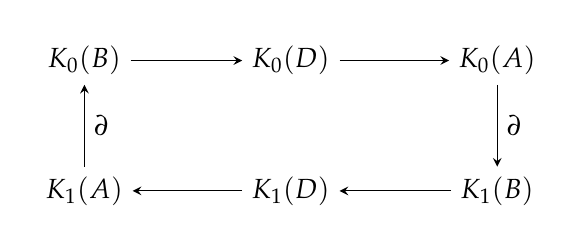
\begin{tikzpicture}
		\matrix (m) [matrix of math nodes,row sep=3em,column sep=4em,minimum width=2em]
		{
			K_0(B) &    K_0(D)&  {K_0(A)}\\
			K_1(A)	& K_1(D)   & K_1(B) \\};
		\path[-stealth]
		(m-1-1) edge node [above] {} (m-1-2)
		(m-1-2) edge node [above] {} (m-1-3)
		(m-2-3) edge node [above] {} (m-2-2)
		(m-2-1) edge node [right] {$\partial$} (m-1-1)
		(m-1-3) edge node [right] {$\partial$} (m-2-3)
		(m-2-2) edge node [above] {}  (m-2-1);
		
	\end{tikzpicture}
	\newline
	
	If $\gamma(\tau)=0$ for an extension $\tau$ then the six-term $K$-theory exact sequence degenerates into two short exact sequences 
	\begin{equation}\nonumber
		0 \to K_j(A) \to K_j(D) \to K_j(B) \to 0 \quad (j=0,1)
	\end{equation}
	and thus determines an element $\kappa(\tau)\in \mathrm{\Ext}^1(K_*(A), K_*(B))$. Homomorphism $\delta$ is inverse to $\kappa$.
	\begin{definition}\label{k_hom_defn}\cite{blackadar:ko}
	If $A$ is a $C^*$-algebra then $K$-\textit{homology} functor $K^*$ is given by $K^*\left( A\right)\bydef KK^*\left( A, \C\right)$. 
	\end{definition}
	\paragraph{!!!}
	\begin{empt}
We now show that the intersection product on KK1 generalizes the pairing
between $K$-theory and $K$-homology. Let $B$ be a trivially graded $\sigma$-unital $C^*$-algebra. If $p$ is a projection in $Q(B)$, then $p$ defines an element $x \in KK\left(\C, B \right)$  as
in 17.6.4. Similarly, if $y \in KK^1\left(B ,\C\right)$ then $y$ may be regarded as an invertible extension $\tau$ of $B$ by  $\K$ (i.e. $\tau B \to Q$) %by 17.6.4. If x 2 M(B)+ with q(x) = p,then e2ix is a unitary in ~B, so ~(e2ix) is a unitary in Q, where ~ is the unitalextension of  to ~B.
	\end{empt}
	\paragraph{!!!}
\begin{definition}\label{busby_defn}\cite{blackadar:ko}
If 
	\be\label{ext_eqn}
0 \to 	B \to D \to A \to 0
\ee
is an extension of $C^*$-algebra, then natural $*$-homomorphism 
	\be\label{busby_eqn}
A \to Q\left(B \right) \bydef M\left(B \right)/B 
\ee
is said to be  the \textit{Busby invariant}.
\end{definition}
\begin{remark}
	The {Busby invariant} uniquely defines the extension up to isomorphism.
\end{remark}
\begin{empt}\label{busby_k_1_empt}\cite{blackadar:ko}  
	It is proven that any $x \in K_1\left(A \right)$ corresponds to a class of isomorphism of extension
	\be\label{ext_k_eqn}
0 \to 	\K \to D \to  A \to 0.
	\ee
	So $x$ can be represented by the Busby invariant
	\be\label{busby_k_eqn}
A \to Q\left(\K \right) \bydef M\left(\K\right)/\K. 
\ee
\end{empt}

\begin{empt}\label{cirle_k1_empt}\cite{blackadar:ko}

	For any $C^*$-algebra $A$ there is a natural homomorphism
	\begin{equation}\label{free_spec_eqn}
		\gamma: K^1(A) \to \mathrm{Hom}(K_1(A), K_0(\mathbb{C})) \approx \mathrm{Hom}(K_1(A), \mathbb{Z})
	\end{equation}
	which is the adjoint of following pairing
	\begin{equation}\nonumber
		KK(\mathbb{C}, A) \otimes KK(A, \mathbb{C}) \to KK(\mathbb{C}, \mathbb{C})\cong\Z.
	\end{equation}
On the other hand  the equation \eqref{free_spec_eqn} comes from \eqref{uct_eqn}.
	If $\tau \in KK^1(A, \mathbb{C})$ is represented by extension
	\begin{equation}\nonumber
		0 \to  \mathbb{C} \to D \to A \to  0
	\end{equation}
	then $\gamma$ is given as connecting maps $\partial$ in the associated six-term exact sequence of $K$ theory
		\newline
	\newline
	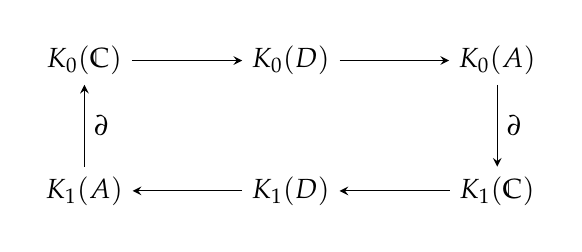
\begin{tikzpicture}
		\matrix (m) [matrix of math nodes,row sep=3em,column sep=4em,minimum width=2em]
		{
		 K_0(\mathbb{C}) &    K_0(D)&  {K_0(A)}\\
	K_1(A)	& K_1(D)   & K_1(\mathbb{C}) \\};
		\path[-stealth]
		(m-1-1) edge node [above] {} (m-1-2)
		(m-1-2) edge node [above] {} (m-1-3)
		(m-2-3) edge node [above] {} (m-2-2)
		(m-2-1) edge node [right] {$\partial$} (m-1-1)
		(m-1-3) edge node [right] {$\partial$} (m-2-3)
		(m-2-2) edge node [above] {}  (m-2-1);
		
	\end{tikzpicture}
	\newline

%\[
%\begin{diagram}
% \node{ K_0(\mathbb{C})) } \arrow{e}  \node{K_0(D)}  \arrow{e}  %\node{K_0(A)}  \arrow{s,r}{\partial}  \\
%\node{K_1(A)} \arrow{n, l}{\partial} \node{K_1(D)} \arrow{w} %\node{K_1(\mathbb{C})} \arrow{w}
%\end{diagram}
%\]	
	If $\gamma(\tau)=0$ for an extension $\tau$ then the six-term $K$-theory exact sequence degenerates into two short exact sequences 
	\begin{equation}\nonumber
		0 \to K_j(A) \to K_j(D) \to K_j(\mathbb{C}) \to 0 \quad (j=0,1)
	\end{equation}
	and thus determines an element $\kappa(\tau)\in \mathrm{\Ext}^1(K_*(A), K_*(\mathbb{C})$. 
	In result we have a sequence of Abelian group homomorphisms
	\begin{equation}\label{uct_c_eqn}
		\mathrm{\Ext}^1(K_0(A), K_0(\mathbb{C})) \to KK^1(A, \mathbb{C}) \to \mathrm{Hom}(K_1(A), K_0(\mathbb{C}))
	\end{equation}
	such that composition of the homomorphisms is trivial. Above sequence can be rewritten by following way
	\begin{equation}\label{uct_c}
		\mathrm{\Ext}^1(K_0(A), \mathbb{Z}) \xrightarrow{\psi} K^1(A) \xrightarrow{\varphi} \mathrm{Hom}(K_1(A), \mathbb{Z})).
	\end{equation}
	If $G$ is an Abelian group that 
	\begin{equation}\nonumber
		\mathrm{\Ext}^1(G, \mathbb{Z}) = \mathrm{\Ext}^1(G_{tors}, \mathbb{Z}),
	\end{equation}
	\begin{equation}\nonumber
		\mathrm{Hom}(G, \mathbb{Z}) =  \mathrm{Hom}(G / G_{tors}, \mathbb{Z})).
	\end{equation}
	From (\ref{uct_c}) it follows that $K^1(A)$ depends on $K_0(A)_{tors}$ and $K_1(A)/K_1(A)_{tors}$. We say that dependence \eqref{uct_c} on $K_0(A)_{tors}$ is a {\it torsion special case} and dependence (\ref{free_spec_eqn}) of $K^1(A)$ on $K_1(A)/K_1(A)_{tors}$ is a {\it free special case}.

	\subsection{Suspensions, mapping cones and Puppe sequences}
	\begin{definition}\label{suspension_defn}\cite{blackadar:ko}
%Definition 8.2.1.
 The \textit{suspension} of $A$, denoted $SA$, is
\be
\left\{f : \R \to A\left|f \quad \mathrm{continuous}, \quad \lim_{x \to \infty }\left\|f\left( x\right)= 0  \right\| \right.\right\}
\ee
 with pointwise  operations and sup norm, $SA$ is a local Banach algebra which is
complete if $A$ is; if $A$ is a $C^*$-algebra, then so is $SA \cong C_0\left( \R\right) \otimes A$. We also say that 	$SA$ is the \textit{algebraic suspension}.
\end{definition}
	\begin{theorem}\label{suspension_thm}\cite{blackadar:ko}
%Theorem 8.2.2. 
$K_1(A)$ is naturally isomorphic to $K_0(SA)$, i .e. there is an isomorphism $\th_A$ : $K_1(A)\to  K_0\left(SA \right)$ such that, whenever $\phi: A\to B$, the
following diagram commutes:
\newline
\begin{tikzcd}
K_1\left(A \right) \arrow[r, "K_1\left(\phi \right)" ]  \arrow[d, "\th_A" ]& K_1\left(B \right)\arrow[d, "\th_B" ]\\ 
K_0\left(SA \right) \arrow[r, "K_0\left(\phi \right)" ] & K_0\left(SB \right)
\end{tikzcd}
\\
(In the language of category theory, $\th$ gives an invertible natural transformation
from $K_1$ to $K_0\circ S$).
\end{theorem}

\begin{definition}\label{mapping_cone_defn}\cite{blackadar:ko}
%Definition 19.4.1. 
\begin{enumerate}
	\item[(a)] If $A$ is a (graded) $C^*$-algebra, the \textit{cone} of $A$, denoted	$CA$, is the (graded) $C^*$-algebra $A \hat \otimes C\left(\left[0, 1\right) \right)  \cong C_0\left(\left[0, 1\right), A \right)$ (with the obvious grading).
	\item[(b)] If $\phi: A\to B$ is a (graded) $*$-homomorphism, then the \textit{mapping cone} of $\phi$,
	denoted $C_\phi$, is the (graded) $C^*$-subalgebra $\left\{\left. \left(x, f \right) \in A\oplus CB\right| \phi\left(x\right) = f\left(0 \right)  \right\}$ of $A\oplus CB$
\end{enumerate}

The mapping cone construction is an important example of a pullback.

\end{definition}
There are maps $p: C_\phi\to A$ and $\iota : SB \to C_\phi$ given by $p(x, f) = x$, $\iota (f) =(0, f)$. (We identify $SB$ with $C_0((0, 1);B)$).
There is a standard short exact sequence 
\be\label{cone_ip_eqn}
0 \to SB \xrightarrow{\iota} C_\phi \xrightarrow{p} A \to 0
\ee
associated to $C_\phi$. The mapping cone construction is natural in $A$ and $B$, i.e. if
we have a commutative diagram
\newline
\begin{tikzcd}
A_1 \arrow[r, "\phi"] \arrow[d, "f"]   & B_1 \arrow[d, "g"] \\
A_2  \arrow[r, "\psi"] & B_2
\end{tikzcd}
\\
there is a map  $\om : C_\phi \to C_\psi$  making the following diagram commutative:
\newline
\begin{tikzcd}
	0 \arrow[r] &SB_1 \arrow[r]\arrow[d, "Sg"]   & C_\phi \arrow[d, "\om"] \arrow[r] & A_1 \arrow[d, "f"]\arrow[r] & 0\\
	0  \arrow[r] & SB_2 \arrow[r]& C_\psi \arrow[r] & A_2 \arrow[r]& 0
\end{tikzcd}

\begin{theorem}\label{puppe_sequence_thm}\cite{blackadar:ko}
%Theorem 19.4.3 
(Puppe Sequences). Let $A$, $B$, $D$ be graded $C^*$-algebras and  $\phi: A\to B$ a graded $*$-homomorphism. Then the following sequences are exact: 
\bean
KK\left(D, SA  \right)\xrightarrow{S{\phi^*}} KK\left(D, SB  \right)\xrightarrow{\iota^*} KK\left(D, C_\phi \right)\xrightarrow{p^*} KK\left(D, A  \right)\xrightarrow{\phi^*}KK\left(D, B  \right),\\
KK\left(B,D  \right)\xrightarrow{\phi^*} KK\left(A, D \right)\xrightarrow{p^*} KK\left( C_\phi, D \right)\xrightarrow{\iota^*} KK\left(SB, D \right)\xrightarrow{S{\phi^*}}KK\left(SA,D  \right).
\eean

\end{theorem}
\end{empt}

\subsection{Fredholm picture of $KK$-theory}
Let $A$ be an  unital, trivially
graded $C^*$-algebra and $B$ is a $\sigma$-unital and trivially graded. We may identify $B\left(\ell^2\left( B\right)  \right)$  with $\mathbb{M}_2\left(  M\left( B \otimes \K\right)\right)$
, with the diagonal-off diagonal grading.% as in 14.1.2(a). 
With this identification, $\phi \bydef \left(\phi_0, \phi_1 \right)$ , where $\phi_j$ is a unital homomorphism from $A$ to $M\left( B \otimes \K\right)$, and
\bean
F \bydef \begin{pmatrix}
	0 & T^*\\
T & 0
	\end{pmatrix}
\eean
for some $T \in  M\left( B \otimes \K\right)$ with $\left\|T \right\|\le 1$ . The intertwining conditions for $F$ and
$\phi$ become $T^*T -1, ~ TT^* - 1, ~ T\phi_1\left(a \right) - \phi_0\left(a \right) \in B\otimes \K$
 for all $a \in A$. The
equivalence relation $\sim_h$ is homotopy of triples $\left(\phi_0, \phi_1, T \right)$   (with strong-operator
continuity).% oh [resp. c] is generated by unitary equivalence, norm-homotopy[resp. compact perturbation] of T, and adding on degenerate triples (where T isa unitary exactly intertwining 0 and 1).
 A Kasparov module in the Fredholm picture is often denoted by a triple
$\left(E^{(0)}\oplus E^{(1)},\phi^{(0)}\oplus \phi^{(1)}  \right) $, where $T \in B\left(E^{(0)}, E^{(1)} \right)$ is an operator with the
right algebraic and intertwining properties as above. Modules expressed in this
way give the \textit{Fredholm picture} of $KK(A,B)$.
\subsection{$KK$-equivalence}
\begin{definition}
%Definition 19.1.1. 
An element $x \in KK(A,B)$ is a $KK$-\textit{equivalence} if there is
$y \in  KK\left( B, A\right)$  with $xy = 1_A$, $yx = 1_B$. $A$ and $B$ are $KK$-\textit{equivalent} if there
exists a $KK$-equivalence in $KK(A,B)$.
 \end{definition}

If $x \in KK\left(A, B \right)$  is a $KK$-equivalence, then for any $D$, $x \hat \oplus_B \left(\cdot \right) KK\left(B, D \right) KK\left(A, D \right)$
 and $\left(\cdot \right)\hat \otimes x :  KK\left(D, A \right) \to KK\left(D, B \right)$ are isomorphisms; these
isomorphisms are natural in $D$ by associativity. So $KK$-equivalent $C^*$-algebras
"behave identically" with regard to $KK$-theory. In particular, if $A$ and $B$ are
trivially graded, right multiplication by $x$ gives an isomorphism from $K_j\left( B\right)\bydef  KK^j\left( \C, B\right)$ , and left multiplication by $y$ gives an isomorphism from $Ext_j\left( A\right)^{-1}  = KK^j\left(A, \C \right)$  to $Ext_j\left( B\right)^{-1}  = KK^j\left(B, \C \right)$
If $x \in KK\left( A, B\right)$  is a $KK$-equivalence with inverse $y$, then $y\check \otimes_A \left(\cdot  \right) \hat \otimes _B y$
a ring-isomorphism from $KK\left( A, A\right)$ onto $KK\left( B, B\right)$
Note that the notion of $KK$-equivalence is only defined for separable %C*$
algebras.

\subsection{Equivariant theory}\label{equiv_k_sec}
\paragraph*{}
Let $A$ be a $C^*$-algebra, $G$ a locally compact group, and a continuous homomorphism
from $G$ into $\Aut\left( A\right)$ , the group of *-automorphisms of $A$ with the
topology of pointwise norm-convergence. A \textit{covariant representation} of the \textit{covariant
system} $\left( A, G, \a\right)$ is a pair of representations $\left(\pi, \rho \right)$  of $A$ and $G$ on the
same Hilbert space such that $\rho\left(g \right) \pi\left( a\right) \left(\rho \right)^* =\pi\left( ga\right)$  for all $a \in A$, $g \in G$,
Let $\left( A, G, \a\right)$  be a covariant system, with $A$ unital. There is an obvious
binary operation on the set of projective $\left( A, G, \a\right)$ -modules, direct sum. There is a category of $\mathbb{V}^G\left( A\right) $ of projective  $\left( A, G, \a\right)$ -modules

\begin{definition}\label{equiv_k_defn}
$K^G_0\left( A\right) $ is the Grothendieck group of $\mathbb{V}^G\left( A\right)$.
\end{definition}

\begin{definition}\label{repr_ring_defn}
	%Definition 11.1.3. 
	The representation ring $R\left(G \right)$  of $G$ is the ring whose elements
	are formal differences of equivalence classes of finite-dimensional representations
	of $G$, with direct sum and tensor product as the ring operations. The
	trivial one-dimensional representation is the multiplicative identity. If $G$ is a finite group then 
	By decomposing a representation into a direct sum of irreducibles, the additive
	group of $R\left(G \right)$  can be identified with $K_0\left(\Z\left[G\right] \right)$.
\end{definition}
\begin{theorem}\label{equiv_k_thm}
Let $\left( A, G, \a\right)$ be a covariant system (with $G$ compact). There
is a natural isomorphism $K^G_0\left( A\right) \cong K_0\left(A\rtimes  G\right)$.
\end{theorem}
\begin{remark}\label{k_repr_rem}
 $K^G_0 (A)$ is not only an Abelian group; it has a natural structure as an $R(G)$-
module, with the action of $\left[W\right]$ sending $p(V \otimes A)$ to $\left(1 \otimes p \right) \left(W\otimes V\otimes A \right)$
Note that if $\C$ is given the trivial $G$-action, then $K_0^G\left(\C \right)\cong R\left(G \right)$.
\end{remark}
\begin{proposition}\label{k_repr_prop}
%Proposition 11.5.2. 
$K^G_0$ is a functor from unital covariant $G$-systems to $R(G)$-
modules.
\end{proposition} 



\begin{theorem}\label{kk_pairing_thm}
%Theorem 20.3.1.   
 Let $A_1$, $A_2$, $B_1$, $B_2$, $D$,  be G-algebras. Then there is a bilinear
pairing
\be\label{kk_pairing_eqn}
\hat \otimes_D: KK^m_G\left(A_1, B_1 \hat \otimes D \right) \times KK^n_G\left(D \hat \otimes A_2, B_2 \right) \to KK^{m+n}\left(A_1 \hat \otimes A_2, B_1 \hat \otimes B_2 \right) 
\ee
which is associative and functorial in all possible senses.
\end{theorem}

\begin{theorem}
%Theorem 20.4.5.
 For any $A$ and $B$, $KK_G\left(A, B \right)$  is an $R_0\left(G \right)$ -module via intersection product. Functoriality of $KK_G$ and the bilinearity of the product respect the module structure, i.e. $KK_G$ is a bifunctor from pairs of $G$-algebras
to $R_0\left( G\right)$ -modules. Similarly, $KK^*_G$
is a bifunctor from pairs of $G$-algebras to
graded $R_*\left(G \right)$ -modules. $KK_G\left(A, A \right)$  is an $R_0\left( G\right)$-algebra; $KK^*_G\left(A, A \right)$ 
is a graded
$R_*\left( G\right)$-algebra.
\end{theorem}
\subsection{Miscellany}	

\begin{proposition}\label{nt_khom_prop}\cite{had:ntk,sudo:ntk}
%Proposition 5. 
For $0\le \th \le 1$, the $K$-homology groups of the $C\left(\T^2_\th \right)$ are $K^j\left(C\left(\T^2_\th \right) \right)\bydef  KK^j\left( C\left(\T^2_\th \right), \C\right) \cong \Z^2$.


\end{proposition}

\section{Inverse limits of $C^*$-algebras}
	

\subsection{Basic constructions}
\paragraph*{}
Inverse limits of $C^*$-algebras are specializations of the explained  in \ref{proj_sys_sec} theory.
	\begin{prop}\label{pro_c_prop}\cite{phillips:inv_lim_app}
		%1.1.1. PROPOSITION. ([63]) 
		Let $A$ be a topological $*$ -algebra over 
		$\C$. Then $A$ is isomorphic, as a topological  $*$ -algebra, to an inverse limit of $C^*$- algebras in the above sense if and only if $A$ is Hausdorff, complete, and its topology 
		is determined by the set of all continuous $C^*$-seminorms on $A$.
	\end{prop}	
	
	\begin{definition}\label{pro_c_defn}\cite{phillips:inv_lim_app}
		%1.1.2. DEFINITION ([53], [7]). 
		A topological $*$-algebra satisfying the 
		conditions of the previous proposition is called a \textit{pro}-$C^*$ -\textit{algebra}. If it is a countable  
		inverse limit of $C^*$-algebras (equivalently, if its topology is determined by countably 
		many continuous $C^*$-seminorms), then it is called a $\sigma$-$C^*$-algebra. 
		
	\end{definition}
	
	\begin{notn}\label{ap_notn}
		If $A$ is a pro-$C^*$-algebra, then $S(A)$ is the set of all	continuous $C^*$-seminorms on $A$, ordered as in the proof of Proposition \ref{pro_c_prop}. For 
		$p\in S\left(A\right)$, we let $\ker(p) \bydef \left\{\left.a\in A\right|p(a)=0\right\}$ and we let $A_p$ be the completion of 
		$A/\ker(p)$ in the norm determined by $p$. It is proven in \cite{phillips:inv_lim} that $A/\ker(p)$ is in fact already complete, so $A/\ker(p)\cong A_p$ is a $C^*$-algebra.  
	\end{notn} 
	Note that $A_p$ is a $C^*$-algebra, and that the proof of Proposition \ref{pro_c_prop} 
	gives a canonical representation of $A$ as an inverse limit, namely $A = \varprojlim_{p\in S(A)} A_p$. 
	%+ Pes(A) (S(A) is directed because if p,^ G S(A), then a   >  max(p(a), q(a)) is also in S(A).) We will show in Corollary 1.2.8 that in fact A/Ker(p) is always already complete.
	\begin{definition}\label{pro_bound_defn}\cite{phillips:inv_lim}
		%1.10. DEFINITION ([63]).
		Let $A$ be a pro-$C^*$-algebra. Then the set of \textit{bounded elements} is the set
		$$
		b\left(A\right)\bydef \left\{ a \in A\left| \left\| a\right\|_\infty = \sup\left\{p\left( a\right)\left| p\in S\left(a\right) \right.\right\}< \infty\right. \right\}.
		$$
		
		%Then an 	element $a\in A$ i s called bounded if $\left\| a\right\|_\infty  \bydef \sup\left\{\left.p(a)\right| p\in S(A)\right\}<\infty$. The set of all 	bounded elements is denoted $b(A)$. 
	\end{definition}
	
	
	\begin{proposition}\label{pro_bound_prop}\cite{phillips:inv_lim_app}
		Let $A$ be a pro-$C^*$-algebra. Then:
		
		\begin{enumerate}
			\item $b\left(A\right)$ is a $C^*$-algebra in the norm $\left\| \cdot\right\|_\infty$.
			\item If $a \in A$ is normal and $f\in C\left(Sp\left(a\right)\right)$ is bounded then $f\left(a\right)\in b\left(A\right)$.
			\item If $a \in A$ is normal then $a\in b\left(A\right)$ if and only if $sp\left(a\right)$ is bounded.
			\item $b\left(A\right)$ is dense in $A$.
			\item For $a\in b\left(A\right)$, we have $sp_{b\left(A\right)}\left(a \right)=\overline{sp_A\left(a \right)}$.
			\item If $q \in S\left(A\right)$ then the map from $b\left(A\right)$ to $A_q$ is surjective.
		\end{enumerate}
		
	\end{proposition}
	
	
	
	\begin{prop}\label{pro_dir_lim_prop}\cite{phillips:inv_lim}
		%3.8
		Direct limits exist in the category of pro-$C^*$-algebras.
	\end{prop}
	\begin{proof}
		If $\left\{A_{\a}\right\}_{\a \in \mathscr A}$ is a direct system of pro-$C^*$-algebras with homomorphisms $\varphi_{\a\bt}: A_\a \to A_\bt$ for $\a\le\bt$ then the direct limit is constructed as follows. Let
		\be\label{seminorms_inv_lim}
		D\bydef\left\{\left. p \in \prod_{\a \in \mathscr A} S\left(A_\a \right)  \right|\forall \a, \bt\in \mathscr A \quad \bt \ge \a \quad p_\bt \circ \varphi_{\a\bt} \le p_\a \right\}
		\ee
		be ordered by $p\le q$ if $p_\a\le q_\a$ for all $\a$. If $p$ denote by the set $B_p \bydef \varinjlim \left( A_\a\right)_p$ and $B = \varprojlim B_p$ then $\varinjlim A_\a$ is the closure of the images of $A_\a$ in $B$.  The complete proof is omitted, because direct limits badly behaved that they do not seem to be of much use.
	\end{proof}
	\begin{remark}\label{pro_dir_lim_rem}
		However direct limits of pro-$C^*$-algebras can be effectively used in the theory of noncommutative coverings (cf. Definition \ref{inv_pro_lim_defn}).
	\end{remark}
	\begin{empt}\label{pro_fin_comp_empt}
		There are explained in \cite{phillips:inv_lim} Hilbert modules over pro-$C^*$-algebras. It is shown that if $E_A$ is a finitely generated module over pro-$C^*$-algebra  $A$  then the  pro-$C^*$-algebra  $\mathcal{L}_A\left( X_A\right)$ adjointable is naturally isomorphic to the algebra $\K\left( X_A\right)$ of  compact operators.
	\end{empt}
	\subsection{Generators and relations}\label{generators_and_relations}
	\paragraph{}
Here I follow to \cite{phillips:inv_lim_app}.	We begin with the construction of the $C^*$-algebra on a properly chosen
	set of generators and relations. Our treatment is based that of \cite{blackadar:shape_theory}, but includes
	changes to make it more suitable for our purposes. If $G$ is any set, we denote by
	$F(G)$ the free associative complex $*$-algebra (without identity) on the set $G$. Thus,
	$F(G)$ consists of all polynomials in the noncommuting variables $C \coprod G^*$ (disjoint union), with complex coefficients and no constant term. By definition, any function
	$p$ from $G$ to a $C^*$-algebra $A$ extends to a unique $*$-homomorphism, which we also
	call $p$, from $F(G)$ to $A$.
	
	A set $R$ of relations on $G$ is a collection of statements about the
	elements of $G$ which make sense for elements of a $C^*$ -algebra. Possible relations
	include statements of the form "$\|x\| \in S$"', where $x \in F(G)$ and $S \in \mathbb{R}$, "$x$ is
	positive," or the statement that some equation in the variables $G \coprod G^*$ and some unknowns has a solution, or that some function from a topological space into $G$ is
	continuous. Note that Blackadar considers only relations of the form $\|x\| \le \eta$ for $\eta > 0$ and $x$ in the unitization $F(G)^+$ of $F(G)$. (We do not allow !!! ADMIT !!! relations involving
	elements of $F(G)^+=F(G)$ because they do not make sense in a nonunital $C^*$-
	algebra. However, it is perfectly possible for $R$ to include the relations $eg = ge   g$
	for some fixed $e \in G$ and all $g \in G \coprod G^*$).
	\begin{definition}\label{gr_ca_defn}\cite{phillips:inv_lim_app}
		Let $(G,R)$ be a set of \textit{generators and relations}.
		(That is, $G$ is a set and $R$ is a set of relations on $G$). Then a \textit{representation} of
		$(G,R)$ in a $C^*$-algebra $A$ is a function $\rho : G \to A$ such that the elements $\rho(g)$ for $g \in G$ satisfy the relations $R$ in $A$. A representation on a Hilbert space $\H$ is a
		representation in $B(\H)$.
	\end{definition} 
	\begin{definition}\label{adm_gr_defn}
		(Compare \cite{blackadar:shape_theory}). A set $(G,R)$ of generators and
		relations is \textit{admissible} if the following conditions hold:
		\begin{enumerate}
			\item The function from $G$ to the zero $C^*$-algebra is a representation of $(G,R)$.
			\item If $\rho$ is a representation of $(G,R)$ in a $C^*$-algebra $A$, and if $B$ is a $C^*$-subalgebra of $A$ which contains $\rho(G)$, then $\rho$ is a representation of $(G,R)$ in $B$.
			\item If $\rho$ is a representation of $(G, R)$ in a $C^*$-algebra $A$, and if $\psi: A\to B$ is a surjective homomorphism, then $\psi \circ \rho$ is a representation of $(G, R)$ in $B$.
			\item For every $g \in G$ there is a constant $M(g)$ such that $\|\rho (g) \| < M(g)$ for all representations $p$ of $(G, R)$.
			\item If $\{\rho_{\alpha}\}$ is a family of representations of $(G, R)$ on Hilbert spaces $\H_{\alpha}$ then $g \mapsto \rho(g)=\oplus_{\alpha}\rho_{\alpha}(g)$   is a representation of $(G, R)$ on $\H= \oplus \H_{\alpha}$. (That is, the elements $\rho(g)$, which are in $B(\H)$ by (4), in fact satisfy the relations $R$.)
		\end{enumerate}
	\end{definition}
	Note that, in the presence of (3), condition (1) is equivalent to "there
	exists a representation of $(G, R)$." Also note that, for relations of the sort considered
	by Blackadar, (2) and (3) are automatic and (5) follows from (4).
	%1.3.3. EXAMPLES, (l) The relation |x|| = 1 on the single generator
	%x does not satisfy (l) of the definition.
	\begin{definition}\label{universal_ca_defn}\cite{phillips:inv_lim_app}
	The \textit{universal $C^*$-algebra on the generators $G$ and relations $R$} is a $C^*$- algebra $C^*(G,R)$ with a representation $\rho$ of $(G,R)$ in $C^*(G,R)$, such that, given any representation $\sigma$ of $(G,R)$ in a $C^*$-algebra $B$, then there is a unique homomorphism
$\psi : C^*(G,R) \to B$ such that $\sigma=\psi \circ \rho$.	
\end{definition}
 If $(G,R)$ is admissible, then $C^*(G,R)$ exists
	and, following Blackadar, can be obtained as the Hausdorff completion of $F(G)$ in the $C^*$ -seminorm $\|x\| = \mathrm{sup}|\rho(x)\|$ where $\rho$ is a representation of $(G,R)$.
	Note that condition (4) guarantees that $\|x\| < \infty$ for $x \in G$, and that condition
	(5) guarantees that the obvious map from $G$ to $C^*(G, R)$ is in fact a representation.
	Admissibility, or something close to it, is also necessary for the existence
	of $C^*(G,R)$. Condition (1) is needed, since otherwise there may be no
	representations at all; conditions (2) and (3) are needed to ensure that the notion of a universal $C^*$-algebra is sensible, and without conditions (4) and (5) it will not be
	possible to construct a universal $C^*$ -algebra. However, if the relations $R$ also make
	sense in a pro-$C^*$ -algebra, then a pro-$C^*$-algebra with the required properties will
	exist under much weaker conditions, as in the following definition. A representation
	of $(G, R)$ in a pro-$C^*$-algebra has the obvious meaning.
	\begin{defn}\label{weak_adm_defn}\cite{phillips:inv_lim_app}
		
		A set $(G, R)$ of generators and relations is called
		\textit{weakly admissible} if the following conditions are satisfied:
		\begin{enumerate}
			
			\item The function from $G$ to the zero $C^*$-algebra is a representation of $(G,R)$.
			\item If $\rho$ is a representation of $(G,R)$ in a $C^*$-algebra $A$, and if $B$ is a $C^*$-subalgebra of $A$ which contains $\rho(G)$, then $\rho$ is a representation of $(G,R)$ in $B$.
			\item If $\rho$ is a representation of $(G, R)$ in a $C^*$-algebra $A$, and if $\varphi: A\to B$ is a surjective homomorphism, then $\varphi \circ \rho$ is a representation of $(G, R)$ in $B$.
			\item For every $g \in G$ there is a constant $M(g)$ such that $\|\rho (g) \| < M(g)$ for all representations $p$ of $(G, R)$.
			\item If $\{\rho_{\alpha}\}$ is a family of representations of $(G, R)$ on Hilbert spaces $\H_{\alpha}$ then $g \mapsto \rho(g)=\oplus_{\alpha}\rho{\alpha}(g)$   is a representation of $(G, R)$ on $\H= \oplus \H_{\alpha}$. (That is, the elements $\rho(g)$, which are in $B(\H)$ by (4), in fact satisfy the relations $R$.)
			
			\item If $A$ is a pro-$C^*$-algebra, and $\rho : G \to A$ is a function such that, for every $p \in S(A)$, the composition of $\rho$ with $A \to A_p$ is a representation of $(G, R)$ in $A_p$, then $\rho$ is a representation of $(G,R)$.
			\item If $\rho_1, ..., \rho_n$ are representations of $(G,R)$ in $C^*$-algebras $A_1,...,A_n$
			then $g \mapsto (\rho_1(g), ..., \rho_n(g))$ is a representation of $(G,R)$ in $A_1 \oplus ... \oplus A_n$.
		\end{enumerate}
	\end{defn}
	\begin{prop}\label{uni_pro_c_rep_prop} \cite{phillips:inv_lim_app}
		Let $(G,R)$ be a weakly admissible set of generators
		and relations. Then there exists a pro-$C^*$ -algebra C*(G,R), equipped with
		a representation $\rho : G \to C^*(G,R)$ of $(G,R)$, such that, for any representation $\sigma$ of $(G,R)$ in a pro-$C^*$-algebra $B$, there is a unique homomorphism $\varphi : C^*(G,R) \to B$
		satisfying $\sigma = \varphi \circ \rho$. If $(G,R)$ is admissible, then $C^*(G,R)$ is a $C^*$-algebra.
	\end{prop}
	\begin{remark}\label{uni_pro_c_rep_rem}
		The construction of $C^*(G,R)$ is described in the proof of the Proposition \ref{uni_pro_c_rep_prop}.  Let $D$ be the set of all $C^*$-seminorms on $F(G)$ of the form 
		$p(x) = \left\|\sigma\left(x \right)  \right\|$  for some representation $\sigma$ of $G$ in a $C^*$-algebra. Then take $C^*(G,R)$ 
		to be the Hausdorff completion of $F(G)$ in the family of $C^*$-seminorms $D$.
	\end{remark}
	
	
	
	\begin{example}\label{wa_exm}\cite{phillips:inv_lim_app}
		%1.3.5. EXAMPLE.
		Any combination (including the empty set) of the 
		following kinds of relations is weakly admissible: 
		\begin{enumerate}
			\item 	Any algebraic relation among  the elements of $F(G)$, or the elements 
			of the $n\times n$ matrix algebra $\mathbb{M}_n\left(F\left( G\right)  \right)$.
			\item Any norm inequality of the form $\left\| x\right\|  < \eta \quad  (\eta \ge 0)$ or $\left\|x\right\| < \eta \quad  (\eta > 0)$, where $x \in F\left( G\right) $. or $x\in \mathbb{M}_n\left(F\left( G\right)  \right)$, and where norm relations are interpreted as 
			applying to all continuous C$*$-seminorms. (Thus, $\left\|x\right\| < 1$ means $p(x) < 1$ for all $p$. 
			Note that this is a weaker condition than $\left\|a\right\|_\infty< 1$).
			\item Any operator inequality $x > 0$ or $x > y$ for $x, y\in \mathbb{M}_n\left(F\left( G\right)  \right)$.
			\item  The assertion that a given function from an appropriate space to 
			$F(G)$ is continuous, Lipschitz, differentiable, continuously differentiate, or r times 
			(continuously) differentiate for $0 < r < \infty$. 
		\end{enumerate}
	\end{example}
	
	
	
	
	\subsection{Commutative pro-$C^*$-algebras}
	\begin{definition}\label{comm_pro_dist_defn}\cite{phillips:inv_lim_app}
		%1.4.1. DEFINITION. 
		Let $\sX$ be a topological space. Then a family $F$ 
		of compact subsets is said to be \textit{distinguished} if it contains all one point sets, is closed 
		under finite unions and passage to compact subsets, and determines the topology in 
		the sense that a subset $C$ of $\sX$ is closed if and only if $C\cap K$ is closed for all $K \in F$. 
		If $\left(\sX_1, F_1\right)$ and  $\left(\sX_2, F_2\right)$ are spaces with distinguished families of compact subsets, 
		then a morphism from  $\left(\sX_1, F_1\right)$ to $\left(\sX_2, F_2\right)$ is a continuous function $f:\sX_1\to\sX_2$ 
		such that $f\left(K\right)\in F_2$ for every $K\in F_1$. 
	\end{definition}
	\begin{empt}\label{comm_pro_dist_empt}\cite{phillips:inv_lim_app}
		If $\sX$ is a topological space, and $F$ is a set of compact subsets of $\sX$, then we 
		write $C_K\left(\sX \right)$  for the topological $*$-algebra of all continuous functions from $\sX$ to $\C$, 
		with the topology of uniform convergence on the members of $F$. If $F$ is omitted, 
		it is understood to be the set of all compact subsets of $F$. Of course, in general 
		$Cont\left( \sX\right)$  can fail to be a pro-$C^*$-algebra by not being complete. We need one more definition. 
	\end{empt}

	\begin{definition}\label{comm_pro_ch_defn}\cite{phillips:inv_lim_app}
		%1.4.2. DEFINITION. 
		We call a topological space $\sX$ \textit{completely Hausdorff}
		for any two distinct points $x,y\in \sX$ there is a continuous function $f: \sX \to \left[0,1\right]$ such that $f(x) = 0$ and $f(y) = 1$. 
		This condition lies between Hausdorff and completely regular. 
	\end{definition}
	
	
	\begin{theorem}\label{comm_pro_thm}\cite{phillips:inv_lim_app}
		%1.4.3. THEOREM ([53]).
		The assignment $\left(\sX, F \right)\mapsto Cont\left( \sX, F\right)$   is a 
		contravariant category equivalence from the category of completely Hausdorff spaces 
		with distinguished families of compact subsets to the category of commutative unital 
		pro-$C^*$-algebras and unital homomorphisms. 
	\end{theorem}
	
	\begin{lemma}\label{comm_pro_lem}\cite{phillips:inv_lim}
		%Corollary 2.9 p 13
		Let $\sX$ be a completely Hausdorff quasitopological space. Then
		$$
		Cont\left(\sX \right) \cong \varprojlim_{K \in F} C\left( K\right). 
		$$
	\end{lemma} 



	\begin{remark}\label{comm_pro_rem}
 Consider  the situation of the Lemma \ref{comm_pro_lem}. If $\sX$  is a topological Hausdorff space then $	Cont\left(\sX \right)$ is a completion of $	C_0\left(\sX \right)$ with respect to a family $\left\{p_K\right\}_{K \in F}$ of seminorms given by
 \be\label{comm_pro_eqn}
p_K\left(a\right)\bydef\max_{ x \in  K}\left| a\left( x \right)  \right|. 
 \ee
\end{remark}
	
	\subsection{Noncommutative suspension and loop space}\label{noncom_loop_space_section}
\paragraph*{}	
	We would like to generalize notion of a loop space.
	%\begin{proof}
	%Let $D$ be the set of all $C^*$-seminorms on $F(G)$ of the form
	%$\rho(x) = \|\sigma(x)\|$ for some representation a of $G$ in a %$C^*$-algebra. Then take $C^*(G,R)$ to be the Hausdorff completion of $F(G)$ in the family of $C^*$-seminorms $D$, with
	%the obvious map $\rho : G \to C^*(G,R)$. To see that $\rho$ is a representation, let $q \in S(C^*(G, R))$. Since $D$ is a directed set in the obvious order (by (5) of the definition
	%of weak admissibility), there is a representation $\sigma$ of $(G,R)$ in a $C^*$-algebra $B$ such
	%that $q(x) < \|\sigma(x)\| \ \forall x \in F(G)$. By (2) we may assume that $B$ is generated by $\sigma(G)$, from which it follows that there is a surjective map $\varphi : B \to C^*(G,R)_q$
	%such that, with $\kappa_q : C^*(G,R) \to C*(G,R)_q$ being the canonical map, we have $\varphi \circ \sigma = \kappa_q \circ \rho$. So $\kappa_q(\rho)$ is a representation by (3), whence p is a representation by
	%(4).
	%To show that $C^*(G,R)$ satisfies the universal property, it suffices, in
	%view of (3), the definition of an inverse limit, and Corollary 1.2.8, to show the universal property holds for representations in C$*$-algebras. Now use the definition of C*{G,R).
	%If $(G,R)$ is admissible, then the directed set $D$ has a largest element
	%$\rho$, so that $C^*(G,R)$ is a $C^*$-algebra with the norm $p$.
	%\end{proof}
		\begin{definition}\label{abelianization_defn}\cite{phillips:inv_lim_app}
%1.5.7 DEFINITION. 
Let $A$ be a pro-$C^*$-algebra. Then the \textit{abelianization} of $A$ is the Hausdorff completion of $A$ in the topology determined by all 
continuous $C^*$-seminorms which vanish on the closed ideal $[A, A]$ generated by all 
commutators $xy - yx$ for $x,y \in  A$. 
The abelianization can also be described as the completion of $A/[A, A]$ 
with respect to the quotient topology, or as the inverse limit $\varprojlim A_p/[A_p, A_p]$. It is 
the largest Abelian quotient of $A$. 	
\end{definition}
\begin{remark}\label{abelianization_rem}
	If $B$ is a commutative pro-$C^*$-algebra then there is the natural bijection $\Hom\left(A, B\right)\cong \Hom\left(A^{\text{ab}}, B\right)$ where $A^{\text{ab}}$ is the abelianization of $A$.
\end{remark}

	
	\begin{definition}\label{pointed_alg_defn}\cite{phillips:inv_lim_app}
%2.5.1. DEFINITION. 
A \textit{pointed} (pro-)$C^*$-algebra is a pair $\left(A,\a)\right)$, where $A$ is a unital (pro-)$C^*$-algebra and $\a : A \to \C$ is a unital homomorphism.
	\end{definition}
	
	\begin{defn}\label{pointed_hom_defn}\cite{phillips:inv_lim_app}
		If $(A, \alpha)$ is a  pointed pro-$C^*$-algebra, than its
		\textit{suspension} is the pro-$C^*$-algebra $\Sigma A = \{f : S^1 \to A \ \mathrm{continuous} \ : \alpha(f(\zeta)) \cdot 1 = f(1), \ \forall \zeta \in S^1\}$, together with the homomorphism $ev_1 : \Sigma A \to \C$ of evaluation at 1. Here $S^1$ is
		identified with $\{\zeta \in \mathbb{C}:|\zeta| = 1\}$. (Note that $ev_1$ makes sense as a homomorphism
		to $\mathbb{C}$ since $f(1) \in \mathbb{C} \cdot 1$ for $f \in \Sigma A$). We also denote by $\left(\Sigma A, ev_1 \right)$ the corresponding  pointed pro-$C^*$-algebra.   
	\end{defn}
	Note that $\Sigma(A^+) = (S A)^+$ , where $SA$ is the conventional suspension $C_0(\mathbb{R} \otimes A$. A left  adjoint for $\Sigma$ in the  pointed category immediately gives a left
	adjoint for $\Sigma$ in the category of pro-$C^*$-algebras and arbitrary homomoprhisms,
	simply by taking the kernel of the homomorphism to $\mathbb{C}$ which comes with the
	 pointed pro-$C^*$-algebra. %It is a left  adjoint for S that Rosenberg really had in	mind, since what he calls $\Sigma$ we call $S$. However, our approach more closely matches the topologists' conventions.
	\begin{defn}\label{pointed_noncommutative_loop_defn}\cite{phillips:inv_lim_app}
		Let $(A, \alpha)$ be a  pointed pro-$C^*$-algebra. We
		construct a  pointed pro-$C^*$-algebra $\Omega A$ in terms of generators and relations as
		follows. Let the generating set $G$ consist of the symbols $z(a, \zeta)$ for a $a \in A$ and $\zeta \in S^1$, and let the relations $R$ be as follows:
		\begin{enumerate}
			\item The map $(a, \zeta) \mapsto z(a, \zeta)$ continuous.
			\item For each fixed $\zeta \in S^1$, the elements $z(a, \zeta)$ satisfy all the algebraic
			relations satisfied by the corresponding elements of $A$.
			\item $z(1,\zeta) = z(1,1)$ $\forall S^1$ .
			\item $z(a, 1) = z(\alpha(a)1, 1)$ $\forall \in  A$.
		\end{enumerate}
		Then set $\Omega A\bydef C^*(G, R)$. The required homomorphism from  $\om_1: \Omega A\to\C$ is given by $z(a, \zeta) \mapsto \alpha(a)$  for $a \in A$ and $\zeta \in S^1$. We say that the pair $\left(\Omega A, \om_1\right)$ is the \textit{ pointed loop algebra} of $(A, \alpha)$.
	\end{defn}
	\begin{thm}\label{nc_s_loop_iso}\cite{phillips:inv_lim_app}
		The map $\Phi : \Hom_+(\Omega A, B) \to \Hom_+(A, \Sigma B)$ defined by $\Phi(\varphi)(a)(\zeta) = \varphi(z((a, \zeta))))$, is a natural bijection, and also defines a natural bijection $[\Omega A,B]^+ \to [A, \Sigma B]^+$ . In particular, $\Omega$ is a left  adjoint for the functor
		$\Sigma$.
	\end{thm}
%	\begin{proof}
%		The statement about homotopy classes follows from the statement		about homomorphisms on replacing $B$ by $B \otimes C([0, 1])$. Therefore we only		consider the statement about homomorphisms. It is sufficient to prove that $\Phi$ defines		a one to one correspondence between  pointed homomorphisms from $A$ to $\Sigma B$		and representations $\rho$ in $B$ of $(G, R)$ which correspond to  pointed homomorphisms		from $\Omega A$ to $B$. If $\beta : B \to \C$ is the homomorphism making $B$ a  pointed algebra,		then the conditions on $\rho$ are $\rho(z(1, 1)) = 1$ and $\beta \circ \rho(z(a, \zeta))= \alpha(a)$ for $a \in A$ and		$\zeta \in S^1$. Using the universal property defining an inverse limit on the isomorphism		$B = \lim_{p \in S(\mathrm{Ker}(\beta))}(\mathrm{Ker}(\beta)_p)^+$ , and conditions (3) and (4) of the definition of weak			admissibility (Definition \ref{weak_adm_defn}), we see that it suffices to consider the case in which		$B$ is a $C^*$-algebra.		\newline		Let $\rho : G \to B$ be a representation of $(G,R)$ such that $\rho(z(1,1)) = 1$		and $\beta \circ \rho(z(a, \zeta))= \alpha(a)$. Define $\psi : A \to \Sigma B$ by $\psi(a)(\zeta) = \rho(z(a, \zeta))$. Then $\psi: A\to \Sigma B$		is certainly a unital $*$-homomorphism satisfying $ev_1(\psi(a)) = \rho(z(a, 1)) = \alpha(a)$, as		desired. (Note that $\psi(a) \in \Sigma B$, by the relations (3) and (4).) That $\psi$ is continuous		follows from relation (l) and the compactness of $S^1$ : if $a_i \to a$ then the joint continuity of $\rho : A \times S^1 \to B$ forces $\rho(z(a_i, \zeta))$ to converge uniformly in $\zeta$ to		$\rho(z(a, \zeta))$. This shows that the definition of $\Phi$ makes sense.		Conversely, let $\psi : A \to \Sigma B$ be a  pointed morphism. Define $p(z(a, \zeta)) = \psi(a)(\zeta)$. Clearly $\rho(z(1, 1)) = 1$ and $\beta \circ \rho ((z(a,\zeta)) = \beta(\psi(a)(\zeta) = \beta(\psi(a)(\zeta) = \alpha(a)$.		Also, the relations of the definition all hold: (l) because $\psi$ is continuous for the supremum norm on $\Sigma B$; (2) because evaluation at $\zeta$ composed with $\psi$ is a homomorphism		for all $\zeta$; (3) because $\psi$ is unital; and (4) because $\psi(a) = \beta(\psi(a)(1)) \cdot 1$ for $a\in A$. 
%	\end{proof} 
	\begin{remark}\label{nc_loop_rem}\cite{phillips:inv_lim_app}
We should note that if $A \bydef C(\sX)$ for some compactly generated
completely Hausdorff space $\sX$, and if $\a = ev_{x_0}$, evaluation at $x_0$, for some $x_0\in\sX$,
then the abelianization of $\Om A$ (Definition \ref{abelianization_defn}) is $C(\Om(\sX,x_0))$, where $\left( \Om\sX, \om_0\right) $ is
the usual loop space of $\sX$ relative to the basepoint (cf. \ref{topological_loop_spaces}), and is equipped
with the compactly generated topology (cf. \ref{top_comp_open_empt}). Note,
however, that $\Om C\left(\sX\right)$ is essentially never commutative, because if $\varphi :\Om A\to \Sigma B$
 is a homomorphism, then there is generally no reason for the ranges of the
homomorphisms $ev_\xi : A \to \Sigma B$ to commute with each other.
\end{remark}
	\section{Local operator spaces}
%	\begin{definition}\label{local_ca_defn}\cite{blackadar:ko}
%3.1.1. 
%A local Banach algebra is a normed algebra $A$ which is closed under holomorphic functional calculus (i.e. if $x\in A$ and $f$ is an analytic function on a neighbourhood of the spectrum of $x$ \textit{in the completion of $A$}, with $f(0) = 0$ if $A$ is nonunital, then $f(x) \in A$.) For technical reasons we will also require that all matrix algebras over $A$ have the same property. If $A$is a $*$-algebra, it will be called a \textit{local Banach $*$-algebra}; if the norm is a pre-$C^*$-norm, $A$ will be called a \textit{local $C^*$-algebra}. 
%	\end{definition}
	\begin{definition}\label{loc_op_sp_defn}\cite{dosi:multi,effros:loc_conv}
		Let $X$ be a linear space and let
		$p^{n} :\mathbb{M}_n(X)\to\left[0, \infty\right]$, $n \in \N$, be gauges (respectively, seminorms) over all matrix spaces. The
		family $p \bydef \left\{p^{n}\right\}_{n\in \N}$ is said to be a \textit{ matrix gauge} (respectively, \textit{matrix seminorm})  on $X$ if
		$p$ possesses the following properties:
		\begin{itemize}
			\item [M1.] $p^{(m+n)}(v \oplus w)= \max\left( p^{(m)}\left(v \right), p^{(n)}\left(w \right)\right) $.
			\item [M2.] $ p^{(n)}\left(avb \right)\le \left\|a \right\|   p^{(m)}\left(v \right)\left\|b \right\| $.
		\end{itemize}
		for all $v = [v_{ij}] \in\mathbb{M}_m(X),~w = [v_{ij}] \in\mathbb{M}_n(E), ~a = [a_{ij}] \in\mathbb{M}_{n,m}(\C),~b = [b_{ij}] \in\mathbb{M}_{m,n}(\C),~ n,m \in\N$. A linear space $X$ with a (separated) family of matrix seminorms $\left\{p_\a\right\}_{\a\in \mathscr A}$ is called an
		\textit{abstract local operator space}. %  We claim that local space should be a closed subspace of multinormed $*$-algebra $A$ such that matrix seminorms of $E$ come from the natural matrix seminorms of $A$.
	\end{definition}
\begin{definition}\label{multinormed_a_defn}\cite{dosi:multi}
A seminorm $p$ on a unital associative algebra $A$ is called a \textit{multiplicative seminorm} if $p(1_A) = 1$ and $p(ab) \le p(a)p(b)$ for all $a, b \in A$. A multiplicative seminorm on an
associative $*$-algebra A is said to be a \textit{$C^*$-seminorm} if $p\left(a^*\right)= p(a)$ and $p\left(a^*a\right)= p(a)^2$ for
all $p\in A$. A complete polynormed  algebra with a defining family of multiplicative seminorms (respectively, $C^*$-seminorms) is called an \textit{Arens Michael algebra} (respectively, \textit{multinormed
$C^*$-algebra}).
\end{definition}
	\begin{remark}\label{la_los_rem}
		Any local operator $C^*$-algebra is an example of a local operator system (cf. \cite{dosi:multi}).
	\end{remark}
		\begin{remark}\label{la_pro_rem}
		Any pro-$C^*$-algebra is an example of a local operator system.
	\end{remark}
		
	\begin{empt}\label{complete_loc_maps_empt}\cite{dosi:multi} 
		Similarly to \ref{complete_maps_empt}  we define a \textit{complete isometry}. 
		\textit{completely contractive} and \textit{complete quotient map}) of abstract local operator spaces.
	\end{empt}
	\begin{definition}\cite{dosi:multi} \label{conc_loc_op_space}
		A \textit{(concrete) local operator space} is a  $\C$-linear subspace $X$ of a multinormed $C^*$-algebra $A$ such that $1_A \in X$. 
	\end{definition}
	\begin{remark}\label{loc_op_abs_conc_rem}\cite{dosi:multi}
		Any local operator space naturally possesses the  structure of an abstract  local operator space. This structure comes from the structure of an abstract  local operator space of multinormed $C^*$-algebra $A$. Conversely  any abstract  local operator space is a concrete  local operator space, i.e. $\C$-subspace of a multinormed $C^*$-algebra.
	\end{remark}
	
	
	\begin{remark}\label{loc_op_sp_rem}
		Any abstract operator local space $V$ is an inverse limit of operator spaces (cf. \cite{dosi:multi} Remark 4.1).
	\end{remark}
	
	
	\section{Locally convex quasi $*$-algebras and their representations}
	
	\paragraph*{}
	Here I follow to \cite{quasi_star}.
	
	\begin{definition}
		%	Definition 2.1.2 
		A \textit{partial $*$-algebra} is a complex vector space $\mathfrak{A}$, endowed with	an involution $a\mapsto a^*$(that is, a bijection, such that $a^{**}=a$, for all $a\in\mathfrak{A}$) and
		a partial multiplication defined by a set $\Ga\subset \mathfrak{A} \times \mathfrak{A}$ (a binary relation), with the	following properties
		\begin{enumerate}
			\item [(a)]	$\left(a,b\right)\in\Ga$ implies $\left(b^*,a^*\right)\in\Ga$;
			\item[(b)] $\left(a,b_1\right),\left(a,b_2\right)\in\Ga$ implies $\left(a,\la b_1 +  \mu bb_2\right)\in\Ga\forall \la,\mu\in\C$;
			\item[(c)] for any $\left(a,b\right)\in\Ga$ , a product $a \cdot b \in \mathfrak{A}$ is defined, which is distributive with 		respect to the addition and satisfies the relation $\left( a^* \cdot b^*\right) = b^*a^*$
		\end{enumerate}
		We shall assume that the partial $*$-algebra $\mathfrak{A}$ contains a unit $e$, if
		$$
		e= e^*, \left( e, a\right) \in \Ga, \forall a\in \mathfrak{A}  \quad \text{and} \quad e \cdot a = a \cdot e = a,\quad  \forall a \in  \mathfrak{A}.
		$$
		If $\mathfrak{A}$ has no unit, it may always be embedded into a larger partial $*$-algebra with unit
		(the so-called unitization of $\mathfrak{A}$), in the standard fashion (cf. \cite{antoine:part_s}).
	\end{definition}
	
	
	\begin{definition}\label{qousi_star_defn}\label{quasi_defn}
		%	Definition 2.1.1 
		A \textit{quasi $*$-algebra} $\left(\mathfrak{A}, \mathfrak{A}_0\right)$ is a pair consisting of a vector space $\mathfrak{A}$
		and a $*$-algebra $\mathfrak{A}_0$ contained in $\mathfrak{A}$ as a subspace, such that
		\begin{itemize}
			\item [(a)] $\mathfrak{A}$ carries an involution $a\mapsto a^*$
			extending the involution of $\mathfrak{A}_0$;
			\item [(b)] $\mathfrak{A}$ is a bimodule over $\mathfrak{A}$ and the module multiplications extend the multiplication
			of $\mathfrak{A}_0$; In particular, the following associative laws hold:
			\be\label{guasi_ass_eqn}
			(xa)y = x(ay);\quad  a(xy) = (ax)y, \quad a \in \mathfrak{A},\quad x,y \in \mathfrak{A}_0; %(2.1.1)
			\ee
			\item [(c)]
			$\left(ax\right)^*=x^*a^*$, for every $a \in \mathfrak{A}$ and $x\in \mathfrak{A}_0$.
		\end{itemize}
		We say that a quasi $*$-algebra $\left(\mathfrak{A}, \mathfrak{A}_0\right)$  is \textit{unital}, if there is an element $e \in \mathfrak{A}_0$,
		such that $ae = a = ea$, for all $a \in \mathfrak{A}$; $e$ is unique and called unit of $\left(\mathfrak{A}, \mathfrak{A}_0\right)$.
		We say that $\left(\mathfrak{A}, \mathfrak{A}_0\right)$ has a \textit{quasi-unit} if there exists an element $q \in \mathfrak{A}$, such that
		$qx = xq = x$, for every $x \in \mathfrak{A}_0$. It is clear that the unit $e$, if any, is a quasi-unit but
		the converse is false, in general.
	\end{definition}
	
	\begin{remark}
		If $\mathfrak{A}$ has no unit, it may always be embedded into a larger partial $*$-algebra with unit
		(the so-called unitization of $\mathfrak{A}$), in the standard fashion \cite{antoine:part_s}.
	\end{remark}
	
	\begin{definition}\label{qousi_star_tau_defn}\cite{quasi_star}
		%Definition 2.2. 
		Let  $\left(\mathfrak{A}, \mathfrak{A}_0\right)$ be a quasi $*$-algebra and $\tau$  a locally convex topology on A. We say that $\left(\mathfrak{A}\left[\tau\right], \mathfrak{A}_0\right)$ is a locally
		convex quasi $*$-algebra if
		\begin{enumerate}
			\item [(a)]  the map $a\in \mathfrak{A} \mapsto a^*\in\mathfrak{A}$ is continuous;
			\item[(b)] for every $x\in \mathfrak{A}_0$, the maps $a \mapsto ax$, $a\mapsto xa$ are continuous in $\mathfrak{A}\left[\tau\right]$;\\
			(c) $\mathfrak{A}_0$ is $\tau$-dense in $\mathfrak{A}$.
		\end{enumerate}
		
	\end{definition}
	\begin{definition}\label{quasi_hom_defn}
		%Definition 2.2.3 
		Let $\left(\mathfrak{A}, \mathfrak{A}_0\right)$ be a quasi $*$-algebra and $\mathfrak{B}$ a partial $*$-algebra (cf. \cite{quasi_star}). A
		linear map 
		from $\mathfrak{A}$ into $\mathfrak{B}$ is called a homomorphism of $\left(\mathfrak{A}, \mathfrak{A}_0\right)$ into $\mathfrak{A}$ if,
		for $a \in\mathfrak{A}$ and $x\in\mathfrak{A}_0$ 
		$\Phi\left(a \right) \Phi\left( x\right)$ and 
		$\Phi\left( x\right) \Phi\left(a \right)$ are well defined in $\mathfrak{B}$ and $\Phi\left( a\right) \Phi\left( x\right)= 
		\Phi(ax)$, 
		$\Phi\left(x \right) \Phi\left(a \right)= 
		\Phi(xa)$, respectively. The homomorphism is called a $*$-\textit{homomorphism} if 
		$\Phi\left(a^*\right)
		) = \Phi\left(a\right)^*$, for every $a\in\mathfrak{A}$.
	\end{definition}
	
	\subsection{Partial $O^*$-algebras}
	\paragraph*{}
	Here I follow to \cite{antoine:part_o}. Define partial $*$-algebras of closable operators in Hilbert spaces. Let $\H$ be a Hilbert space with inner product $\left(\cdot, \cdot\right)_\H$ and $\D$ a dense subspace of $\H$. We denote by $\L\left(\D, \H \right)$ the set of all closable linear 
	operators $X$ in $\H$ such that $\D\left(X \right)  =\D$ and put
	\be\label{l_dag_eqn}
	\begin{split}
		\L\left( \D\right) \bydef\left\{\left.X\in \L\left(\D, \H \right)\right|X\D\subset \D \right\},\\
		\L^\dagger\left( \D, \H\right) \bydef\left\{\left.X\in \L\left(\D, \H \right)\right|\D\left(X^* \right)\supset \D \right\},\\
		\L^\dagger\left( \D\right) \bydef\left\{\left.X\in \L^\dagger\left(\D, \H \right)\cap \L\left( \D\right) \right|X^*\D\subset \D \right\}.
	\end{split}
	\ee
	Then $\L^\dagger\left( \D, \H\right)$ is a vector space 
	with the usual operations: $X + Y$, $\la X$, and $\L\left(\D \right)$ is a subspace of $\L^\dagger\left( \D, \H\right)$ and 
	an algebra with the usual 
	multiplication $XY$
	For $\L^\dagger\left(\D, \H \right)$ 
	and $\L^\dagger\left(\D\right)$, we 
	have 
	the following
	\begin{proposition}\cite{antoine:part_o}
		$\L^\dagger\left(\D, \H \right)$ is a partial $*$-algebra with respect to the following operations: the sum $X + Y$, the scalar multiplication $\la X$, the involution $X\mapsto X^\dagger\bydef X^*|_\D$  and the (weak) partial multiplication $X\Hsquare Y\bydef X^{\dagger *} Y$, defined whenever $X$ is a left  multiplier of $Y$, ($X \in L^{\mathrm{w}}\left(Y \right)$ or $Y \in R^{\mathrm{w}}\left(X \right)$), that is, iff $Y\D\subset\D\left(X^{\dagger *} \right)$ and $X^\dagger\D\subset \D\left( Y^*\right)$. $\L^\dagger\left(\D\right)$ is a $*$-algebra 
		with the usual multiplication $XY$ (which here coincides with the weak multiplication $\Hsquare$) and the involution $X \mapsto X^\dagger$.
	\end{proposition} 
	\begin{remark}\label{o*b_rem}
		If 
		\be
		\begin{split}\label{o*b_eqn}
			\L^\dagger\left( \D, \H\right)_b\bydef\left\{\left.X\in \L^\dagger\left( \D, \H\right)\right|\overline{X}\in B\left(\H \right) \right\},\\
			\L^\dagger\left( \D\right)_b\bydef \L^\dagger\left( \D, \H\right)_b\cap \L^\dagger\left(\D \right) 
		\end{split}
		\ee
		then the  inclusion $\L^\dagger\left( \D, \H\right)_b\subset B\left(\H \right)$ induces a norm  on $\L^\dagger\left( \D, \H\right)_b$ which is a $C^*$-norm on $\L^\dagger\left( \D\right)_b$.
	\end{remark}
	
	\begin{definition}\label{o*alg_defn}\cite{antoine:part_o}
		A subset (subspace) of $\L^\dagger\left( \D, \H\right)$ is 
		called an $O$-\textit{family} ($O$-\textit{vector space}) 
		on $\D$, and a subalgebra of $\L\left( \D\right)$
		is called an $O$-\textit{algebra} on $\D$. A $\dagger$-
		invariant subset (subspace) of subset (subspace) of $\L^\dagger\left( \D, \H\right)$ is 
		called an $O^*$-\textit{family} ($O^*$-\textit{vector space}) 
		on $\D$. A partial $*$-subalgebra of $\L^\dagger\left( \D, \H\right)$ is called a \textit{partial} $O^*$-\textit{algebra} on $\D$, and a 
		$*$-subalgebra of  $\L^\dagger\left( \D\right)$ is 
		called an $O^*$-\textit{algebra} on $\D$. 
	\end{definition}
	\begin{remark}\label{*_bound_rem}
		If $A$ is a  $O^*$-\textit{algebra} on $\D$, i.e, 
		$A \subset \L^\dagger\left( \D\right)$ then the subalgebra
		\be\label{*_bound_eqn}
		A_b \bydef A\cap \L^\dagger\left( \D\right)_b
		\ee
		and $C^*$-norm on 	it depend on multiplication and $*$-operation on $A$. The $*$-algebra	$A_b$
		and $C^*$-norm on 	it do not depend in the inclusion $A \subset \L^\dagger\left( \D\right)$
	\end{remark}
	
	
	\subsection{Quasi $*$-algebras and partial $*$-algebras of operators}
	\paragraph{}
	Let $\D$ be a dense subspace of a Hilbert space $\H$.
	We denote by $\L^\dagger\left( \D, \H\right)$  the set of all (closable) linear operators $X$ in $\H$, such that $D\left( X\right) = \D$, $D\left( X^*\right)\supseteqq \D$ where $D\left( X\right)$ denotes the domain of $X$. The set $\L^\dagger\left( \D, \H\right)$ is a partial $*$-algebra with respect to the following operations:
	the usual sum $X_1 + X_2$, the scalar multiplication $\la X$, the involution $X \mapsto X^\dagger\bydef X^*\D$ and the (weak) partial multiplication $X1\square X_2\bydef X_1^{\dagger *}
	X_2$ (where $X_1^{\dagger *}\bydef  \left( X_1^{\dagger}\right)^*$). The latter is defined whenever $X_2$ is a \textit{weak right multiplier} of  $X_2$ (for this, we shall write $X_2\in R^w\left( X_1\right) $ or  $X_1\in L^w\left( X_1\right) $, that is, if and only if, $X_2\D\subset D\left(X_1^{\dagger *}\right)$ and $X_1^\dagger\D\in D\left(X_2^* \right)$. The operator $1_\D$, restriction to $\D$ of the identity
	operator $1_\H$ on $\H$, is the unit of the partial $*$-algebra $\L^\dagger\left( \D, \H\right)$. By $\L^\dagger\left( \D, \H\right)_b$ we shall denote the bounded part of $\L^\dagger\left( \D, \H\right)$; i.e.,
	$$
	\L^\dagger\left( \D, \H\right)_b\bydef\left\{\left.X\in \L^\dagger\left( \D, \H\right)\right|\overline{X}\in B\left(\H \right) \right\}
	$$
	where $\overline{X}$ is the closure of $X$, i.e., a minimal closed extension of $X$.
	Let us denote by $\L^\dagger\left(\D \right)$  the space of all linear operators $X:\D\to\D$, having an adjoint $X^\dagger : \D\to\D$, by which we simply mean that 
	$$
	\left(X\xi, \eta\right)= \left(\xi, X^\dagger\eta\right)\quad\forall \xi, \eta\in \D.
	$$
	If $\L^\dagger\left( \D, \H\right)$ is endowed with the strong $*$-topology $\mathrm{t}_{s^*}$ , defined by the set of seminorms
	$$
	p_\xi(X)\bydef \left\| X\xi\right\|  + \left\| X^\dagger\xi\right\| \quad \xi\in \D, \quad  X\in \L^\dagger\left( \D, \H\right),
	$$
	then $\left(\L^\dagger\left( \D, \H\right)\left[\mathrm{t}_{s^*}\right],\L\dagger(D)_b)\right)$ is a locally convex quasi $*$-algebra or, more precisely, a \textit{locally convex quasi $C^*$-normed algebra}.
	If $\L^\dagger\left( \D, \H\right)$ is endowed with the weak topology $\mathrm{t}_w$ defined by the set of seminorms
	$$
	p_{\xi,\eta}(X)\bydef \left| \left(X\xi, \eta \right) \right|   \quad \xi, \eta\in \D, \quad  X\in \L^\dagger\left( \D, \H\right),
	$$
	then, again, $\left(\L^\dagger\left( \D, \H\right)\left[\mathrm{t}_{w}\right],\L\dagger(D)_b)\right)$. is a locally convex quasi $*$-algebra.
	\begin{definition}
		%Definition 2.2.5 
		Let $\left(\mathfrak{A}, \mathfrak{A}_0\right)$ be a quasi $*$-algebra and $\D_\pi$ a dense domain in a
		certain Hilbert space $\H_\pi$ . A linear map $\pi$ from $\mathfrak{A}$ into $\L^\dagger\left(\H_\pi, \D_\pi \right)$ is called a
		$*$-representation of $\left(\mathfrak{A}, \mathfrak{A}_0\right)$, if the following properties are fulfilled:
		\begin{enumerate}
			\item [(a)] $\pi\left( a^*\right) = \pi\left( a\right)^\dagger\quad \forall a \in pi\left( a^*\right)$.
			\item[(b)]  for $a\in \mathfrak{A}$ and $x\in \mathfrak{A}$ $\pi\left( a\right)\square \pi\left( x\right)$  is well defined and $\pi\left( a\right)\square \pi\left( x\right)=\pi\left(ax \right)$ 
		\end{enumerate}
		
		In other words,  $\pi$ is a $*$-homomorphism of $\left(\mathfrak{A}, \mathfrak{A}_0\right)$ into the partial $*$-algebra
		$\L^\dagger\left(\D_\pi, \H_\pi \right)$
		
		If $\left(\mathfrak{A}, \mathfrak{A}_0\right)$ has a unit $e \in \mathfrak{A}_0$, we assume $\pi\left(e \right)  = \Id_{\D_\pi}$, where $\Id_{\D_\pi}$ is the identity operator on the space $\D_\pi$. If $\pi_o\bydef\pi|_{ \mathfrak{A}_0}$  is a $*$-representation of the $*$-algebra $\mathfrak{A}_0$ into $\L^\dagger\left(\D_\pi \right) $ we say that $\pi$ is a qu$*$-representation.
	\end{definition}
	
	\begin{empt}If
		$$
		\mathfrak{A}^+_0\bydef\left\{\sum_{k=1}^n x^*_kx_k\quad x_k \in  \mathfrak{A}_0\quad n\in \N \right\}
		$$
		
		then, $\mathfrak{A}^+_0$ is a wedge in $\mathfrak{A}_0$ and we call the elements of $\mathfrak{A}^+_0$ \textit{positive elements} of $\mathfrak{A}_0$. We call \textit{positive elements} of $\mathfrak{A}\left[\tau\right]$ the elements of closure (with respect to $\tau$) of  $\mathfrak{A}^+_0$ in 
		and we denote them by $\mathfrak{A}^+$.
		
	\end{empt}
	\begin{proposition}
		If $a \ge 0$, then $\pi\left(a \right)\ge 0$ , for every $\left(\tau,\mathrm{t}_{w} \right)$-continuous $*$-representation of $\left(\mathfrak{A}\left[\tau\right], \mathfrak{A}_0\right)$.
	\end{proposition}
	\begin{theorem}
		%Theorem 6.2.2 
		Assume that $\mathfrak{A}^+\cap \left(-\mathfrak{A}^+\right)= \{0\}$. Let $a \in \mathfrak{A}^+$, $a\neq 0$. Then, there
		exists a continuous linear functional $\om$ on $\mathfrak{A}\left[\tau\right]$ with the properties:
		\begin{enumerate}
			\item[(i)] $\om\left(b \right)\ge 0\quad \forall b \in \mathfrak{A}^+$;
			\item[(ii)] $\om\left(a \right)> 0$.
		\end{enumerate}
		
	\end{theorem}
	
	If $\left(\mathfrak{A}\left[\tau\right], \mathfrak{A}_0\right)$ is an arbitrary locally convex quasi $*$-algebra then there is a natural order related to the topology $\tau$. This order can be  used to define bounded elements. In what follows, we shall assume that $\left(\mathfrak{A}\left[\tau\right], \mathfrak{A}_0\right)$
	has a unit $a$. Let $a\in \mathfrak{A}$; put  $\mathfrak{R}\left( a\right)\bydef \frac{1}{2}\left(a + a^* \right)$ $\mathfrak{J}\left( a\right)\bydef \frac{1}{2i}\left(a - a^* \right)$
	Then, $\mathfrak{R}\left( a\right),\mathfrak{J}\left( a\right) \in\mathfrak{A}_h$ and $a = \mathfrak{R}\left( a\right)+i\mathfrak{J}\left( a\right)$
	\begin{definition}
		%Definition 6.4.1 
		An element $a\in $ is called \textit{order bounded} if there exists $\ga \ge 0$, such that 
		$$\pm \mathfrak{R}\left( a\right) \le \ga e,\quad \pm \mathfrak{J}\left( a\right) \le \ga e$$.
		We denote by $\mathfrak{A}^{\mathrm{or}}_{\mathrm{b}}$
		b the set of all order bounded elements of $\mathfrak{A}\left[\tau\right]$.
	\end{definition}
	
	
	We recall that an unbounded $C^*$-seminorm $p$ on a partial $*$-algebra $\mathfrak{A}$ is a seminorm defined on a partial $*$-subalgebra $D(p)$ of $\mathfrak{A}$, the domain of $p$, with the properties:
	\begin{itemize}
		\item $p(ab)   p(a)p(b)$, whenever $ab$ is well-defined;
		\item $p\left(a^*a \right) = p\left(a \right)^2$  whenever $a^*a$ is well-defined
	\end{itemize}
	
	\begin{proposition}
		%Proposition 6.4.14 
		$\left\|\cdot \right\|^{\mathrm{or}}_{\mathrm{b}}$ is an unbounded $C^*$-norm on $\mathfrak{A}$ with domain $\mathfrak{A}_b$.
	\end{proposition}
\section{Representations by unbounded operators on Hilbert modules}
\label{sec:rep_Hilbert_module}
\paragraph*{} 
Let $A $ be a unital $*$-algebra,  $D $ a $C^*$-algebra,
and $\mathcal{E} $ a Hilbert  $D $-module.  

\begin{definition}
	\label{def:rep_Hilbert_module}\cite{meyer:unb_repr}
	A \emph{representation} of $A $ on $\mathcal{E} $ is a
	pair $(\mathfrak{E},\pi) $, where  $\mathfrak{E}\subseteq\mathcal{E} $ is a dense
	$D $-submodule and  $\pi\colon A\to\End_D(\mathfrak{E}) $ is a unital
	algebra homomorphism to the algebra of  $D$-module endomorphisms
	of $\mathfrak{E} $, such that
\be\label{def:rep_Hilbert_module_eqn}
	\braket{\pi(a)\xi}{\eta}_D = \braket{\xi}{\pi(a^*)\eta}_D
	\qquad
	\text{for all }a\in A,\ \xi,\eta\in\mathfrak{E}.
\ee
	
	We call $\mathfrak{E} $ the \emph{domain} of the representation.  We
	may drop $\pi $ from our notation by saying that $\mathfrak{E} $ is an
	$A,D $-bimodule with the right module structure inherited
	from $\mathcal{E} $, or we may drop $\mathfrak{E} $ because it is the common
	domain of the partial linear maps $\pi(a) $ on $\mathcal{E} $ for all
	$a\in A $.
	We equip $\mathfrak{E} $ with the \emph{graph topology}, which is
	generated by the \emph{graph norms}
	\be	\label{graph_norm_eqn}
	\left\| {\xi}\right\| _a \bydef \left\langle \xi, \xi\right\rangle^{\nicefrac12}  + \left\langle  \pi(a)\xi,\pi(a)\xi\right\rangle^{\nicefrac12}	= \left\langle  \xi,\pi(1+a^*a)\xi\right\rangle ^{\nicefrac12}
	\ee
	for  $a\in A $.  The representation is \emph{closed} if $\mathfrak{E} $
	is complete in this topology.  A \emph{core} for $(\mathfrak{E},\pi) $ is
	an  $A,D $-subbimodule of $\mathfrak{E} $ that is dense in $\mathfrak{E} $ in
	the graph topology.
\end{definition}

Definition~\ref{def:rep_Hilbert_module}  for  $D=\C $ is the usual
definition of a representation of a $*$-algebra on a Hilbert
space by unbounded operators.   For  $\mathcal{E}=D $ with the
canonical Hilbert  $D $-module structure, we get representations
of $A $ by \emph{densely defined unbounded multipliers}.  The
domain of such a representation is a dense right ideal
$\mathfrak{E}\subseteq D $.  

Given two norms  $p,q $, we write  $p \preceq q $ if there is a
scalar  $c>0 $ with  $p \le c q $.

\begin{lemma}
	\label{lem:graph_norms_directed}\cite{meyer:unb_repr}
	The set of graph norms partially ordered by $\preceq $ is
	directed: for all  $a_1,\dotsc,a_n\in A $ there are  $b\in A $ and
	$c\in\R_{>0} $ so that  $\mathrm{norm}{\xi}_{a_i} \le c\mathrm{norm}{\xi}_b $ for
	any representation  $(\mathfrak{E},\pi) $, any  $\xi\in\mathfrak{E} $, and
	$i=1,\dotsc,n $.
\end{lemma}




\begin{definition}%[\cite{Pal:Regular},	\cite{Lance:Hilbert_modules}*{Chapter 9}]
	\label{def:regular}
	A densely defined operator $t $ on a Hilbert module $\mathcal{E} $ is
	\emph{semiregular} if its adjoint is also densely defined; it is
	\emph{regular} if it is closed, semiregular and  $1+t^*t $ has dense
	range.  An \emph{affiliated multiplier} of a
	$C^*$-algebra $D $ is a regular operator on $D $ viewed as
	a Hilbert  $D $-module.
\end{definition}



The usual norm on $\mathcal{E} $ is the graph norm for  $0\in A $.  Hence
the inclusion map  $\mathfrak{E}\hookto\mathcal{E} $ is continuous for the graph
topology on $\mathfrak{E} $ and extends continuously to the
completion $\overline{\mathfrak{E}} $ of $\mathfrak{E} $ in the graph topology.

\begin{proposition}
	\label{pro:closure_rep}
	The canonical map  $\overline{\mathfrak{E}}\to\mathcal{E} $ is injective, and its
	image is
	\begin{equation}
		\label{eq:domain_closure}
		\overline{\mathfrak{E}} = \bigcap_{a\in A} \Dom \overline{\pi(a)}.
	\end{equation}
	Thus $(\mathfrak{E},\pi) $ is closed if and only if  $\mathfrak{E} =
	\bigcap_{a\in A} \Dom \overline{\pi(a)} $.  Each  $\pi(a) $ extends
	uniquely to a continuous operator $\overline{\pi(a)} $
	on $\overline{\mathfrak{E}} $.  This defines a closed
	representation $(\overline{\mathfrak{E}},\overline{\pi}) $ of $A $, called the
	\emph{closure} of $(\mathfrak{E},\pi) $.
\end{proposition}


We shall need a generalisation of~\eqref{eq:domain_closure} that
replaces $A $ by a sufficiently large subset.

\begin{definition}
	\label{def:strong_generating_set}
	A subset  $S\subseteq A $
	is called a \emph{strong generating} set if it generates $A $
	as an algebra and the graph norms for  $a\in S $
	generate the graph topology in any representation.  That is, for any
	representation on a Hilbert module, any vector $\xi $
	in its domain and any  $a\in A $,
	there are  $c\ge1 $
	in $\R $
	and  $b_1,\dotsc,b_n\in S $
	with  $\mathrm{norm}{\xi}_a \le c \sum_{i=1}^n \mathrm{norm}{\xi}_{b_i} $.
\end{definition}

An estimate  $\mathrm{norm}{\xi}_a \le c \sum_{i=1}^n \mathrm{norm}{\xi}_{b_i} $
is usually shown by finding  $d_1,\dotsc,d_m\in A $
with
$a^* a + \sum_{j=1}^m d_j^* d_j = c\cdot \sum_{i=1}^n b_i^* b_i $,
compare the proof of Lemma~\ref{lem:graph_norms_directed}.

\begin{proposition}
	\label{pro:equality_if_closure_equal}
	Let  $S\subseteq A $ be a strong generating set.  Two closed
	representations  $(\mathfrak{E}_1,\pi_1) $ and $(\mathfrak{E}_2,\pi_2) $
	of $A $ on the same Hilbert module $\mathcal{E} $ are equal if and
	only if  $\overline{\pi_1(a)} = \overline{\pi_2(a)} $ for all  $a\in S $.
\end{proposition}

Here we consider 

\begin{corollary}
	\label{cor:bounded_rep}
	Let $S $ be a strong generating set of $A $ and
	let $(\mathfrak{E},\pi) $ be a closed
	representation of $A $ with  $\Dom \overline{\pi(a)} = \mathcal{E} $ for each
	$a\in S $.  Then  $\mathfrak{E}=\mathcal{E} $ and $\pi $ is a
	$*$-homomorphism to the $C^*$-algebra  $\mathbb{B}(\mathcal{E}) $ of
	adjointable operators on $\mathcal{E} $.
\end{corollary}


An \emph{isometry}  $I\colon \mathcal{E}_1\hookto\mathcal{E}_2 $
between two Hilbert  $D $-modules  $\mathcal{E}_1 $
and $\mathcal{E}_2 $
is a right  $D $-module
map with  $\braket{I\xi_1}{I\xi_2} = \braket{\xi_1}{\xi_2} $
for all  $\xi_1,\xi_2\in\mathcal{E}_1 $.

\begin{definition}
	\label{def:isometric_intertwiner}
	Let  $(\mathfrak{E}_1,\pi_1) $
	and  $(\mathfrak{E}_2,\pi_2) $
	be representations on Hilbert  $D $-modules
	$\mathcal{E}_1 $
	and $\mathcal{E}_2 $,
	respectively.  An \emph{isometric intertwiner} between them is an
	isometry  $I\colon \mathcal{E}_1\hookto\mathcal{E}_2 $
	with  $I(\mathfrak{E}_1)\subseteq \mathfrak{E}_2 $
	and  $I\circ\pi_1(a) (\xi) = \pi_2(a) \circ I (\xi) $
	for all  $a\in A $,
	$\xi\in\mathfrak{E}_1 $;
	equivalently,  $I\circ\pi_1(a)\subseteq \pi_2(a)\circ I $
	for all  $a\in A $,
	that is, the graph of $\pi_2(a)\circ I $
	contains the graph of $I\circ \pi_1(a) $.
	We neither ask $I $
	to be adjointable nor  $I(\mathfrak{E}_1)=\mathfrak{E}_2 $.
	Let  $\mathrm{Rep}(A,D) $
	be the category with closed representations of $A $
	on Hilbert  $D $-modules
	as objects, isometric intertwiners as arrows, and the usual
	composition.  The unit arrow on $(\mathfrak{E},\pi) $
	is the identity operator on $\mathcal{E} $.
\end{definition}

\begin{lemma}
	\label{lem:closure_functorial}
	Let  $(\mathfrak{E}_1,\pi_1) $ and  $(\mathfrak{E}_2,\pi_2) $ be
	representations on Hilbert  $D $-modules  $\mathcal{E}_1 $
	and $\mathcal{E}_2 $, respectively, and let  $I\colon
	\mathcal{E}_1\hookto\mathcal{E}_2 $ be an isometric intertwiner.  Then $I $ is
	also an intertwiner between the closures of  $(\mathfrak{E}_1,\pi_1) $
	and  $(\mathfrak{E}_2,\pi_2) $.
\end{lemma}
\begin{proposition}
	\label{pro:intertwiner_strong_generators}
	Let  $(\mathfrak{E}_1,\pi_1) $ and  $(\mathfrak{E}_2,\pi_2) $ be closed
	representations of $A $ on Hilbert  $D $-modules  $\mathcal{E}_1 $
	and $\mathcal{E}_2 $, respectively.  Let  $S\subseteq A $ be a strong
	generating set.  An isometry  $I\colon \mathcal{E}_1\hookto \mathcal{E}_2 $ is
	an intertwiner from  $(\mathfrak{E}_1,\pi_1) $ to  $(\mathfrak{E}_2,\pi_2) $
	if and only if  $I\circ \overline{\pi_1(a)} \subseteq \overline{\pi_2(a)}\circ
	I $ for all  $a\in S $.
\end{proposition}


Now we relate the categories  $\mathrm{Rep}(A,D) $ for different
$C^*$-algebras $D $.

\begin{definition}
	\label{def:Cstar-correspondence}
	Let  $D_1 $ and $D_2 $ be two $C^*$-algebras.  A
	\emph{$C^*$-correspondence} from $D_1 $ to $D_2 $ is a
	Hilbert  $D_2 $-module with a representation of $D_1 $ by
	adjointable operators (representations of $C^*$-algebras are
	tacitly assumed nondegenerate).  An \emph{isometric intertwiner}
	between two correspondences from $D_1 $ to $D_2 $ is an
	isometric map on the underlying Hilbert  $D_2 $-modules that
	intertwines the left   $D_1 $-actions.  Let  $\mathrm{Rep}(D_1,D_2) $
	denote the category of correspondences from $D_1 $ to $D_2 $
	with isometric intertwiners as arrows and the usual composition.
\end{definition}


Let $\mathcal{E} $ be a Hilbert  $D_1 $-module and $\F $ a
correspondence from $D_1 $ to $D_2 $.  The interior tensor product
$\mathcal{E}\otimes_{D_1} \F $ is the (Hausdorff) completion of the
algebraic tensor product  $\mathcal{E}\odot \F $ to a Hilbert
$D_2 $-module, using the inner product
\begin{equation}
	\label{eq:interior_tensor}
	\braket{\xi_1\otimes\eta_1}{\xi_2\otimes\eta_2}
	= \braket{\eta_1}{\braket{\xi_1}{\xi_2}_{D_1}\cdot\eta_2}_{D_2}.
\end{equation}
We may use the balanced tensor product
$\mathcal{E}\odot_{D_1} \F $ instead of  $\mathcal{E}\odot \F $
because the inner product~\eqref{eq:interior_tensor} descends to this
quotient.  If we want to emphasise the left  action  $\varphi\colon
D_1\to\mathbb{B}(\F) $ in the
$C^*$-correspondence $\F $, we write  $\mathcal{E}\otimes_\varphi
\F $ for  $\mathcal{E}\otimes_{D_1} \F $.

In addition, let $(\mathfrak{E},\pi) $ be a closed representation of $A $
on $\mathcal{E} $.  We are going to build a closed representation
$(\mathfrak{E}\otimes_{D_1}\F, \pi\otimes_{D_1}1) $ of $A $ on
$\mathcal{E}\otimes_{D_1}\F $.  First let  $X\subseteq
\mathcal{E}\otimes_{D_1}\F $ be the image of  $\mathfrak{E}\odot \F $
or  $\mathfrak{E}\odot_{D_1} \F $ under the canonical map to
$\mathcal{E}\otimes_{D_1}\F $.

\begin{lemma}
	\label{lem:tensor_rep_with_corr}
	For  $a\in A $, there is a unique linear operator
	$\pi(a)\otimes1\colon X\to X $ with  $(\pi(a)\otimes1)
	(\xi\otimes\eta) = \pi(a)(\xi)\otimes \eta $ for all
	$\xi\in\mathfrak{E} $,  $\eta\in\F $.  The map  $a\mapsto
	\pi(a)\otimes 1 $ is a representation of $A $ with domain $X $.
\end{lemma}

\begin{definition}
	Let  $(\mathfrak{E}\otimes_{D_1}\F, \pi\otimes_{D_1}1) $ be the
	closure of the representation on $\mathcal{E}\otimes_{D_1}\F $
	defined in Lemma~\ref{lem:tensor_rep_with_corr}.
\end{definition}

\begin{lemma}
	\label{lem:rep_tensor_corr_functor}
	Let  $I\colon \mathcal{E}_1\hookto\mathcal{E}_2 $ be an isometric intertwiner
	between two representations  $(\mathfrak{E}_1,\pi_1) $ and
	$(\mathfrak{E}_2,\pi_2) $, and let  $J\colon \F_1\hookto \F_2 $
	be an isometric intertwiner of $C^*$-correspondences.  Then
	$I\otimes_{D_1} J\colon \mathcal{E}_1\otimes_{D_1}\F_1 \hookto
	\mathcal{E}_2\otimes_{D_1}\F_2 $ is an isometric intertwiner between
	$(\mathfrak{E}_1\otimes_{D_1}\F_1, \pi_1\otimes1) $ and
	$(\mathfrak{E}_2\otimes_{D_1}\F_2, \pi_2\otimes1) $.
\end{lemma}

The lemma gives a bifunctor
\begin{equation}
	\label{eq:interior_tensor_bifunctor}
	\otimes_{D_1}\colon \mathrm{Rep}(A,D_1)\times \mathrm{Rep}(D_1,D_2) \to
	\mathrm{Rep}(A,D_2).
\end{equation}
The corresponding bifunctor
\[
\otimes_{D_1}\colon \mathrm{Rep}(B,D_1)\times \mathrm{Rep}(D_1,D_2) \to \mathrm{Rep}(B,D_2)
\]
for a $C^*$-algebra $B $ is the usual composition of
$C^*$-correspondences.  This composition is associative up to
canonical unitaries
\begin{equation}
	\label{eq:tensor_associative}
	\mathcal{E} \otimes_{D_1} (\F \otimes_{D_2} \mathcal{E}) \xrightarrow{\cong}
	(\mathcal{E} \otimes_{D_1} \F) \otimes_{D_2} \mathcal{E},\qquad
	\xi \otimes (\eta\otimes \zeta) \mapsto
	(\xi \otimes \eta)\otimes \zeta,
\end{equation}
for all triples of composable $C^*$-correspondences.

\begin{lemma}
	\label{lem:tensor_associative}
	If $\mathcal{E} $ carries a representation $(\mathfrak{E},\pi) $ of a
	$*$-algebra $A $, then the unitary
	in~\eqref{eq:tensor_associative} is an intertwiner  $(\mathfrak{E},\pi)
	\otimes_{D_1} (\F\otimes_{D_2} \mathcal{E}) \xrightarrow{\cong}
	\bigl((\mathfrak{E},\pi) \otimes_{D_1} \F\bigr) \otimes_{D_2}
	\mathcal{E}$.
\end{lemma}

\begin{definition}
	\label{def:star-intertwiner}
	Let  $(\mathfrak{E}_1,\pi_1) $ and $(\mathfrak{E}_2,\pi_2) $ be two
	representations of $A $ on Hilbert  $D $-modules  $\mathcal{E}_1 $
	and $\mathcal{E}_2 $.  An adjointable operator  $x\colon
	\mathcal{E}_1\to\mathcal{E}_2 $ is an \emph{intertwiner} if
	$x(\mathfrak{E}_1)\subseteq \mathfrak{E}_2 $ and  $x\pi_1(a)\xi =
	\pi_2(a)x\xi $ for all  $a\in A $,  $\xi\in\mathfrak{E}_1 $.  It is
	a \emph{$*$-intertwiner} if both  $x $ and $x^* $ are
	intertwiners.
	\label{def:adjointable_intertwiner}
\end{definition}

Any adjointable intertwiner between two representations of a
$C^*$-algebra $B $ is a $*$-intertwiner.  In contrast, for
a general $*$-algebra, even the adjoint of a unitary
intertwiner $u $ fails to be an intertwiner if
$u(\mathfrak{E}_1)\subsetneq \mathfrak{E}_2 $.

\begin{example}
	\label{exa:Friedrichs_extension}
	Let $t $ be a positive symmetric operator on a Hilbert
	space $ \H $.  Assume that  $\bigcap_{n\in\N} \Dom t^n $ is
	dense in $ \H $, so that $t $ generates a
	representation $\pi $ of the polynomial algebra $\C[x] $
	on $ \H $.  The Friedrichs extension of $t $ is a positive
	self-adjoint operator $t' $ on $ \H $.  It generates
	another representation $\pi' $ of $\C[x] $ on $ \H $.  The
	identity map on $ \H $ is a unitary intertwiner
	$\pi\hookto\pi' $.  It is not a $*$-intertwiner unless
	$t=t' $.
\end{example}

The following proposition characterises when an adjointable isometry
$I\colon \mathcal{E}_1\hookto \mathcal{E} $ between two representations
on Hilbert  $D $-modules is a $*$-intertwiner.  Since
$\mathcal{E}\cong \mathcal{E}_1 \oplus \mathcal{E}_1^\bot $ if $I $ is adjointable, we
may as well assume that $I $ is the inclusion of a direct summand.

\begin{proposition}
	\label{pro:isometry_star-intertwiner}
	Let  $\mathcal{E}_1 $ and $\mathcal{E}_2 $ be Hilbert modules over a
	$C^*$-algebra $D $ and let  $(\mathfrak{E}_1,\pi_1) $ and
	$(\mathfrak{E},\pi) $ be representations of $A $ on  $\mathcal{E}_1 $
	and $\mathcal{E}_1\oplus\mathcal{E}_2 $, respectively.  The following are
	equivalent:
	\begin{enumerate}
		\item \label{enum:isometry_star-intertwiner1} the canonical
		inclusion  $I\colon \mathcal{E}_1\hookto\mathcal{E}_1\oplus\mathcal{E}_2 $ is a
		$*$-intertwiner from $\pi_1 $ to $\pi $;
		\item \label{enum:isometry_star-intertwiner2} the canonical
		inclusion  $I\colon \mathcal{E}_1\hookto\mathcal{E}_1\oplus\mathcal{E}_2 $ is an
		intertwiner from $\pi_1 $ to $\pi $ and  $\mathfrak{E} =
		\mathfrak{E}_1 + (\mathfrak{E}\cap \mathcal{E}_2) $;
		\item \label{enum:isometry_star-intertwiner3} there is a
		representation  $(\mathfrak{E}_2,\pi_2) $ on $\mathcal{E}_2 $ such that  $\pi
		= \pi_1 \oplus \pi_2 $.
	\end{enumerate}
\end{proposition}

\begin{definition}\cite{meyer:unb_repr}
		\label{def:Cstar-hull}
		A {\it $C^*$-hull} for the integrable representations
		of~\(A\) is a $\Cstar$-algebra~\(B\) with a family of bijections
		\(\Phi=\Phi^{\E}\) from the set of representations of~\(B\)
		on~\(\E\) to the set of integrable representations of~\(A\)
		on~\(\E\) for all Hilbert modules~\(\E\) over all
		$C^*$-algebras~\(D\) with the following properties:
		\begin{itemize}
			\item \emph{compatibility with isometric intertwiners}: an isometry
			$\E_1 \hookto \E_2$ (not necessarily adjointable) is an
			intertwiner between two representations \(\varrho_1\)
			and~\(\varrho_2\) of~\(B\) \emph{if and only if} it is an
			intertwiner between \(\Phi(\varrho_1)\) and~\(\Phi(\varrho_2)\);
			
			\item \emph{compatibility with interior tensor products}: if
			$\F$ is a correspondence from~\(D_1\) to~\(D_2\),
			\(\E\) is a Hilbert \(D_1\)-module, and~\(\varrho\) is a
			representation of~\(B\) on~$\F$, then
			$\Phi(\varrho\otimes_{D_1} 1_{\F}) =
			\Phi(\varrho)\otimes_{D_1} 1_{\F}$ as representations
			of~\(A\) on \(\E\otimes_{D_1} \F\).
		\end{itemize}
	
	
\end{definition}

\begin{definition}
	\label{def:weak_Cstar-hull}
	A {\it weak $C^*$-hull} for the integrable representations
	of~\(A\) is a $C^*$-algebra~\(B\) with a family of
	bijections~\(\Phi\) between representations of~\(B\) and integrable
	representations of~\(A\) on Hilbert modules that is compatible with
	unitary $*$-intertwiners and interior tensor products.
\end{definition}

\begin{proposition}
	\label{pro:unique_hull}
	A class of integrable representations has at most one weak
	$C^*$-hull.
\end{proposition}

\subsection{Universal enveloping algebras of Lie algebras}
\label{sec:Ug}

We illustrate our theory by an example.  Let~\(\mathfrak{g}\) be a
finite-dimensional Lie algebra over~\(\R\) and let \(A=U(\mathfrak{g})\) be
its universal enveloping algebra with the usual involution, where
elements of~\(\mathfrak{g}\) are skew-symmetric.  A representation of~\(A\)
on~\(\E\), possibly not closed, is equivalent to a dense
submodule \(\mathfrak{C}\subseteq\E\) with a Lie algebra representation
\(\pi\colon \mathfrak{g}\to\Endo_D(\mathfrak{C})\) satisfying
\(\braket{\xi}{\pi(X)(\eta)} = -\braket{\pi(X)(\xi)}{\eta}\) for all
\(X\in\mathfrak{g}\), \(\xi,\eta\in\mathfrak{C}\).

Let~\(G\) be a simply connected Lie group with Lie algebra~\(\mathfrak{g}\)
and let \(B\defeq \Cst(G)\).  A representation of~\(\Cst(G)\) on a
Hilbert module~\(\E\) is equivalent to a strongly continuous,
unitary representation of~\(G\) on~\(\E\).  Given such a
representation, let~\(\E^\infty\subseteq \E\) be its subspace
of smooth vectors.  This is the domain of a closed representation
of~\(U(\mathfrak{g})\).  We call a representation of~\(U(\mathfrak{g})\) integrable if
it comes from a unitary representation of~\(G\) in this way.

In particular, \(G\) acts continuously on~\(\Cst(G)\) by left
multiplication with unitary multipliers.  Let
\(\mathfrak{B}=\Cst(G)^\infty\) be the right ideal of smooth elements
for this \(G\)-action, equipped with the canonical
\(U(\mathfrak{g})\)-module structure~\(\mu\).  By the universal property
of~\(\Cst(G)\), the pair \((\mathfrak{B},\mu)\) is the universal
integrable representation.  That is, a representation of~\(U(\mathfrak{g})\)
is integrable if and only if it is of the form \((\mathfrak{B},\mu)
\otimes_\varrho \E\) for a representation~\(\varrho\)
of~\(\Cst(G)\).

Let \(X_1,\dotsc,X_d\) form a basis of~\(\mathfrak{g}\).  The
\emph{Laplacian} is \(L\defeq -\sum_{i=1}^d X_i^2 \in U(\mathfrak{g})\).

\begin{theorem}[\cite{Pierrot:Reguliers}*{Th�or�me 2.12}]
	\label{the:integrable_Ug}
	A representation \((\pi,\mathfrak{C})\) of~\(U(\mathfrak{g})\) is integrable if
	and only if~\(\cl{\pi(L^n)}\) is regular and self-adjoint for all
	\(n\in\N\).
\end{theorem}

\begin{theorem}
	\label{the:Cstar_hull_Lie_algebra}
	The class of integrable representations of~\(U(\mathfrak{g})\)
	has~\(\Cst(G)\) as a $C^*$-hull and is defined by submodule
	conditions.  So it satisfies the Strong Local--Global Principle.
\end{theorem}


The results of Vassout~\cite{Vassout:Unbounded_groupoids} get close
to proving an analogue of Theorem~\ref{the:Cstar_hull_Lie_algebra}
for an \(s\)-simply connected Lie groupoid~\(G\) with compact base.
This analogue would
replace~\(\mathfrak{g}\) by the space of smooth sections of the Lie
algebroid~\(A(G)\), and \(U(\mathfrak{g})\) by the \Star{}-algebra of
\(G\)-equivariant differential operators on~\(G\), a subalgebra
of the \Star{}-algebra of \(G\)-pseudodifferential operators.  Any
symmetric, elliptic element of~\(U(\mathfrak{g})\) should be a possible
replacement for the Laplacian in
Theorem~\ref{the:Cstar_hull_Lie_algebra}.
\subsection{Lie algebroids}
\begin{lem}\cite{Vassout:Unbounded_groupoids}
Lemma 37. Let P be a pseudodifferential operator of order m with real part m0. Then P is in
L(Hm0,E) and L(E,H
?m0 ).
\end{lem}


\section{Discrete crossed product of $C^*$-algebras}\label{discr_cr_prod_sec}	
Here I follow to \cite{discrete_crossed}.
Let $G$ be a discrete group and $A$ a $C^*$-algebra. An action of $G$ on $A$ is a group homomorphism from $G$ into $\Aut(A)$   the group of $*$-automorphisms on $A$. The action is denoted by a dot in the following way
$$
t \mapsto (a \mapsto t. a),\quad t \in G,\quad a \in A.
$$
A $C^*$-dynamical system $(A,G)$ consist of a discrete group $G$, a $C^*$-algebra $A$ and an action of $G$ on $A$. For a $C^*$-dynamical system $(A,G)$ with $G$ discrete let $C_c(G,A)$ be the linear span of finitely supported functions on G with values in $A$. A typical element a in $C_c(G,A)$ is written as a sum
\be\label{discr_cr_prod_cc_eqn}
\sum _{t \in G} a_t u_t\quad \forall t \in G \quad a_t  \in A,
\ee
where only finitely many $a_t$ s are non-zero. One equips $C_c(G,A)$ with a $*$-operation and a twisted product, in such
a way that the action becomes  inner . By this we mean that $t. a = u_tau^*_t$ for every $t \in G$, $a \in A$. More precisely we have the following product and $*$-operation
\be\label{discr_cr_prod_op_eqn}
\begin{split}
	ab \bydef \sum_{s,t\in G}a_t(t\cdot b_s)u_{ts}, \quad
	a^* =\sum_{t\in G} (t^{-1}.a^*_t )u_{t^{-1}} ,\\ a =\sum _{t \in G} a_t u_t, \quad b =\sum _{s \in G} a_s u_s
\end{split}
\ee
Fix a $C^*$-dynamical system $(A,G)$ with $G$ discrete. A covariant representation $\left(\pi, u, \H \right)$  of $(A,G)$ consists of an unitary representation $u: G \to B(\H)$ of $G$ and a representation $\pi  : A \to B(\H)$ of $A$ such that $u(t) (a)u(t)^* = \pi(t. a)$
for every $t \in  G$ and $a \in A$. For a covariant representation $\left(\pi, u, \H \right)$ let $\pi\times u$ denote the associated representation of $C_c(G,A)$ on $\H$. The \textit{full $C^*$-algebra norm} on $C_c(G,A)$ is given by
$$
\left\|\cdot \right\|  \bydef \sup\left\| (\pi \times u)(\cdot )\right\| 
$$
where the supremum is taken over all covariant representations  $\left(\pi, u, \H \right)$ of $(A,G)$. The \textit{full crossed product}, denoted $A \rtimes  G$, is the completion of
$C_c(G,A)$ with respect to the full $C^*$-algebra norm.
The \textit{reduced $C^*$-algebra norm} on $C_c(G,A)$ is given by
\be\label{discr_red_n_eqn}
\left\|\cdot \right\|_\la  \bydef \sup\left\| \widetilde\pi \times \la(\cdot )\right\|
\ee
where the regular representation $\widetilde\pi : C_c(G,A) \to B(\widetilde \H )$ is the representation associated to the covariant representation given by 
\be\label{discr_red_repr_eqn}
\widetilde\pi\left(\delta_{t, \xi} \right) \bydef \delta_{t, \pi\left(t^{-1}.a\right) \xi}\quad \la(s)\delta_{st, \xi} \bydef \delta_{t, \xi}, \quad a \in A, \quad t, s \in G, \quad \xi \in \H
\ee
where $\pi: A \hookto B\left(\H\right)$ is any faithful representation, $\widetilde \H\bydef \ell^2\left(G, \H\right) $ and $\delta_{t, \xi}$ is the map $s \mapsto \delta_{t, s}\xi \in \H$ ($ \delta_{t, s}$ is the Kronecker delta). In this way $\widetilde\pi$ becomes faithful. The reduced $C^*$-algebra norm does not depend on the choice of the faithful representation $\pi$ (cf.  \cite{discrete_crossed}). The \textit{reduced crossed product}, denoted by $A\rtimes_rG$ is the completion of $C_c(G,A)$ with respect to the reduced $C^*$-algebra norm. 

%  (a)t, = t, (t1.a), (s)t, = st,, a  A, s, t  G,   H where   : A  B(H) is any faithful representation, H = l2(G,H) andt,  H is the map s 7 t,s  H (t,s is the Kronecker delta). In thisway      becomes faithful, cf. [61, Lemma 2.26]. The reduced C$*$-algebranorm does not depend on the choice of the faithful representation  , cf. [9,Proposition 4.1.5]The reduced crossed product, denoted ArG, is the completion of Cc(G,A)with respect to the reduced C$*$-algebra norm. The inclusion of G into thegroup of unitaries inM(ArG) allow !!! ADMIT !!!s us to consider ut, t  G as an unitary element in M(A r G), cf. [61, Proposition 2.34].Let ( , u,H) be a covariant representation of a C$*$-dynamical system (A,G) with G discrete. Then  u extends to a representation  u of AGon H. The map sending ( , u,H) into    u is a one-to-one correspondencebetween covariant representations of (A,G) and representations of AG, cf.[61, Proposition 2.40].Let us proof a few results to give the reader a better understanding ofsome of the well known results about crossed product C$*$-algebras.


\chapter{Spectral triples}
	
	\paragraph{}
	This section contains citations of  \cite{hajac:toknotes}. 
	\section{Definition of spectral triples}\label{sp_tr_defn_sec}
	\begin{defn}
		\label{df:spec-triple}\cite{hajac:toknotes}
		A (unital) {\it {spectral triple}} $(\A, \H, D)$ consists of:
		\begin{itemize}
			\item
			an unital pre-$C^*$-algebra $\A$ with an involution $a \mapsto a^*$, equipped
			with a faithful representation on:
			\item
			a \emph{Hilbert space} $\H$; and also
			\item
			a \emph{self-adjoint operator} $D$ on $\mathcal{H}$, with dense domain
			$\Dom D \subset \H$, such that $a(\Dom D) \subseteq \Dom D$ for all 
			$a \in \mathcal{A}$.
		\end{itemize}
	\end{defn}
	\begin{defn}
		\label{df:spt-real_defn}\cite{hajac:toknotes}
		A {\it real  spectral triple} is a  spectral triple $(\sA, \sH, D)$,
		together with an antiunitary operator $J\:\sH\to\sH$ such that
		$J(\Dom D)\subset \Dom D$, and 
	\be\label{df:spt-real_eqn}
	[a, Jb^*J^\dagger] = 0
	\ee for all
		$a, b \in \sA$.
	\end{defn}
	
	\begin{defn}
		\label{df:spt-even}\cite{hajac:toknotes}
		A  spectral triple $(\sA, \sH, D)$ is {\it even} if there is
		a selfadjoint unitary \textit{grading operator} $\Ga$ on $\sH$ such that $a\Ga = \Ga a$
		for all $a \in \sA$, $\Ga(\Dom D) = \Dom D$, and $D\Ga = -\Ga D$. If
		no such $\bZ_2$-grading operator $\Ga$ is given, we say that
		the spectral triple is {\it odd}.
	\end{defn}
	There is a set of axioms for  spectral triples described in \cite{hajac:toknotes,varilly:noncom}. In this article the following axioms are used only.
	\begin{axiom}\label{regularity_axiom}\cite{varilly:noncom} (Regularity). 
		For any $a \in \A$, $[D,a]$ is a bounded operator on~$\H$, and both
		$a$ and $[D,a]$ belong to the domain of smoothness
		$\bigcap_{k=1}^\infty \Dom(\delta^k)$ of the derivation $\delta$
		on~$B(\H)$ given by $\delta(T) \stackrel{\mathrm{def}}{=} [\left|D\right|,T]$.
	\end{axiom}
	\begin{axiom}\label{finiteness_axiom}
		(Finiteness)
		The subspace of smooth vectors
		$\sH^\infty \bydef \bigcap_{k\in\bN} \Dom D^k$ is a \emph{finitely
			generated projective} left  $\sA$-module.
		
		This is equivalent to saying that, for some $N \in \bN$, there is a 
		projector $p = p^2 = p^*$ in~$M_N(\sA)$ such that 
		$\sH^\infty \isom \sA^N p$ as left  $\sA$-modules. 
	\end{axiom}
	\begin{axiom}[Real structure]
		The antiunitary operator $J : \sH \to \sH$ satisfying
		$J^2 = \pm 1$, $JDJ^\dagger = \pm D$, and $J\Ga = \pm \Ga J$ in the even
		case, where the signs depend only on $n \bmod 8$ (and thus are given
		by the table of signs for the standard commutative examples).
		\[
		\begin{array}[t]{|c|cccc|}
			\hline
			n \bmod 8               & 0 & 2 & 4 & 6 \rule[-5pt]{0pt}{17pt} \\
			\hline
			J^2 = \pm 1             & + & - & - & + \rule[-5pt]{0pt}{17pt} \\
			JD = \pm D J & + & + & + & + \rule[-5pt]{0pt}{17pt} \\
			J\Ga = \pm\Ga J         & + & - & + & - \rule[-5pt]{0pt}{17pt} \\
			\hline
		\end{array}
		\qquad\qquad
		\begin{array}[t]{|c|cccc|}
			\hline
			n \bmod 8               & 1 & 3 & 5 & 7 \rule[-5pt]{0pt}{17pt} \\
			\hline
			J^2 = \pm 1             & + & - & - & + \rule[-5pt]{0pt}{17pt} \\
			JD = \pm D J & - & + & - & + \rule[-5pt]{0pt}{17pt} \\
			\hline
		\end{array}
		\]
		Moreover , $b \mapsto J b^* J^\dagger$ is an antirepresentation of $\sA$
		on~$\sH$ (that is, a representation of the opposite algebra
		$\sA^\opp$), which commutes with the given representation of~$\sA$:
		\be\label{st_comn_eqn}
		[a, J b^* J^\dagger] = 0,  \word{for all} a,b \in \sA,
		\ee
		(cf. Definition \ref{df:spt-real_defn}).
	\end{axiom}
	
	
	\begin{axiom}\label{fist_order_st_ax}(First order).
		For each $a,b \in \sA$, the following relation holds:
		\begin{equation}\label{fist_order_eqn}
			[[D, a], J b^* J^\dagger] = 0,  \word{for all} a,b \in \sA.
		\end{equation}
		This generalizes, to the noncommutative context, the condition that
		$D$ be a first-order differential operator.
		Since 
		\[
		[[D, a], Jb^*J^\dagger]
		= [[D, Jb^*J^\dagger], a] + [D, \underbrace{[a, Jb^*J^\dagger]}_{=0}],
		\]
		this is equivalent to the condition that 
		\be\label{first_order_dual_eqn}
		[a, [D, Jb^*J^\dagger]] = 0.
		\ee
	\end{axiom}
	

\begin{axiom}[Orientation]\label{orientation_st_ax}
	There is a Hochschild $n$-cycle
	$$
	\cc = \tsum_j (a_j^0 \ox b_j^0) \ox a_j^1 \oxyox a_j^n 
	\in Z_n(\sA, \sA \ox \sA^\opp),
	$$
	such that
	\begin{equation}\label{eq:vol-cond}
		\pi_D(\cc)
		\equiv \tsum_j a_j^0 (J b_j^{0*} J^{-1}) \,[D,a_j^1] \dots [D,a_j^n]
		= \begin{cases} \Ga, &\text{if $n$ is even}, \\
			1, &\text{if $n$ is odd}. \end{cases}
		\end{equation}
\end{axiom}

	
	\begin{lem}
		\label{lm:proj-approx}\cite{hajac:toknotes}
		Let $\sA$ be an unital Fr\'echet pre-$C^*$-algebra, whose
		$C^*$-completion is~$A$. If $\tilde{q} = \tilde{q}^2 = \tilde{q}^*$ is
		a projection in $A$, then for any $\eps > 0$, we can find a projection
		$q = q^2 = q^* \in \sA$ such that $\|q - \tilde{q}\| < \eps$.
	\end{lem}
	\begin{theorem}\label{smooth_k_iso_thm}\cite{varilly_bondia}
		If $\sA$ is  a Fr\'echet pre-$C^*$-algebra with $C^*$-completion $A$, then the inclusion $j: \A \to A$ induces an isomorphism $K_0\left( j\right) : K_0\left(\A\right)\to K_0\left(A\right)$.
	\end{theorem}
	\begin{remark}\label{smooth_k_iso_rem}
		The $K_0$-symbol in the above Theorem is the $K_0$-functor of $K$-theory (cf. \cite{bass,blackadar:ko}). The $K_0$-functor is related to projective finitely generated modules. Otherwise any projective finitely generated module corresponds to the idempotent of the matrix algebra. The idea of the proof of the Theorem \ref{smooth_k_iso_thm} contains following ingredients:
		\begin{itemize}
			\item For any idempotent $\tilde e \in \mathbb{M}_n\left(A\right)$ one constructs and idempotent $e\in \mathbb{M}_n\left(\A\right)$ such that there is the isomorphisms $\tilde e A^n\cong e A^n$ of $A$-modules.
			\item The inverse to $K_0j$ homomorphism is roughly speaking given by
			$$
			\left[e\A^n\right]\mapsto \left[ \tilde e A^n\right] 
			$$
			where $\left[\cdot \right]$ means the $K$-theory class  of projective finitely generated module. From the isomorphism $\tilde e A^n\cong e A^n$ the above equation can be replaced with
			\be\label{smooth_k_iso_eqn}
			\left[e\A^n\right]\mapsto \left[  e A^n\right]
			\ee
		\end{itemize}
	\end{remark}
	\section{Representations of  smooth algebras}\label{s_repr}
	
	\paragraph*{}
	Let $(\A, \H, D)$ be a spectral triple. Similarly to \cite{bram:atricle} we  define a representation of $\pi^1:\A \to B(\H^2)$ given by
	\begin{equation}\label{s_diff1_repr_equ}
		\pi^1(a) =  \begin{pmatrix} a & 0\\
			[D,a] & a\end{pmatrix}.
	\end{equation}
	We can inductively construct  representations $\pi^s: \A \to B\left(\H^{2^s}\right)$ for any $s \in \mathbb{N}$. If $\pi^s$ is already constructed then  $\pi^{s+1}: \A \to B\left(\H^{2^{s+1}}\right)$ is given by
	\begin{equation}\label{s_diff_repr_equ}
		\pi^{s+1}(a) =  \begin{pmatrix}  \pi^{s}(a) & 0 \\ \left[D,\pi^s(a)\right] &  \pi^s(a)\end{pmatrix}
	\end{equation}
	where we assume diagonal action of $D$ on $\H^{2^s}$, i.e.
	\begin{equation*}
		D \begin{pmatrix} x_1\\ ... \\ x_{2^s}
		\end{pmatrix}= \begin{pmatrix} D x_1\\ ... \\ D x_{2^s}
		\end{pmatrix}; \ x_1,..., x_{2^s}\in \H.
	\end{equation*}
	For any $s \in \N^0$ there is a seminorm $\left\|\cdot \right\|_s$  on $\A$ given by
	\begin{equation}\label{s_semi_eqn}
		\left\|a \right\|_s = \left\| \pi^{s}(a) \right\|.
	\end{equation}
	The definition of spectral triple requires that $\A$ is a Fr\'echet algebra with respect to seminorms $\left\|\cdot \right\|_s$.
	
	
	\section{Noncommutative differential forms}\label{ass_cycle_sec}

	\paragraph*{} 
	\begin{defn}\cite{connes:ncg94}\label{cycle_defn}
		\begin{enumerate}
			\item [(a)]  A \textit{cycle} of dimension $n$ is a triple $\left(\Om, d, \int \right)$ where $\Om = \bigoplus_{j=0}^n\Om^j$  is a graded algebra over $\C$, $d$ is a graded derivation of degree 1 such that $d^2=0$, and $\int :\Om^n \to \C$ is a closed graded trace on $\Om$,
			\item[(b)] Let $\A$  be an algebra over $\C$. Then a \textit{cycle over } $\A$ is given by a cycle $\left(\Om, d, \int \right)$	and a homomorphism $\A \to \Om^0$.
		\end{enumerate}
	\end{defn}
	\begin{empt}\label{connes_cycle_empt}
		We  let $\Om^*\A$ be the reduced universal differential graded algebra over $\A$ (cf. \cite{connes:ncg94} Chapter III.1).
		It is by definition equal to $\A$ in degree 0 and is generated by symbols $da$ ($a \in \A$) of
		degree 1 with the following presentation:
		\begin{enumerate}
			\item[$(\a)$] $d(ab) = (da)b + adb \quad \forall a, b \in \A$,
			\item[$(\bt)$] $d1 = 0$.
		\end{enumerate}
		
		One can check that $\Om^1\A$ is isomorphic as an $\A$-bimodule to the kernel $\ker(m)$ of the
		multiplication mapping $m : \A\otimes\A \to A$, the isomorphism being given by the mapping
		$$
		\sum a_j \otimes b_j \in \ker(m) \mapsto \sum a_j d b_j\in \Om^1\A
		$$
		The involution * of $\A$ extends uniquely to an involution on * with the rule
		$$
		\left(da \right)^* \stackrel{\text{def}}{=} - da^*.
		$$
		The differential $d$ on $A$ is defined unambiguously by
		$$
		d(a_0da_1 ... da_n) =  da_0da_1 ... da_n \quad \forall a_j \in \A,
		$$
		and it satisfies the relations
		\bean
		d^2\om = 0 \quad \forall \om \in \Om^*\A,\\
		d(\om_1\om_2) = (d\om_1)\om_2 + \left( -1\right)^{\partial \om_1} \om_1 d\om_2.
		\eean
		
	\end{empt}
	\begin{proposition}\label{st_cycle_connes_prop}\cite{connes:ncg94}
		Let  $\left( \A, \H, D\right)$  be a spectral triple.
		\begin{enumerate}
			\item 	The following equality defines a $*$-representation $\pi$ of the reduced universal
			algebra $\Om^*\A$ on $\H$:
			\be\label{diff_repr_eqn}
			\pi(a_0da_1 ... da_n) = a_0[D, a_1] ... [D, a_n] \quad \forall a_j \in \A.
			\ee
			\item Let $J_0 = \ker \pi$  be the graded two-sided ideal of $\Om^*\A$ given by 
			\be\label{junk_grad_eqn}
			J_0^k = \left\{\left.\om \in \Om^k~\right| \pi\left(\om \right)=0 \right\}
			\ee
			then 
			\be\label{junk_cycle_eqn}
			J = J_0 + dJ_0
			\ee
			is a graded differential two-sided ideal of
			$\Om^*\A$.
		\end{enumerate}
	\end{proposition}
	\begin{remark}
		Using 2) of Proposition \ref{st_cycle_connes_prop}, we can now introduce the graded differential algebra
		\be\label{connes_cycle_eqn}
		\Om_D \bydef \Om^*\A/J.
		\ee
	\end{remark}
	
	Thus any spectral triple $\left( \A, \H, D\right)$  naturally defines a cycle $\rho : \A \to \Om_D$ (cf. Definition \ref{cycle_defn}). 
	In particular for any spectral triple there is an $\A$-bimodule $\Om^1_D\subset B\left(\H \right) $ of differential forms which is the $\C$-linear span of operators given by
	\begin{equation}\label{dirac_d_module}
		a\left[D, b \right];\quad a,b \in \A.
	\end{equation}
	There is the differential map
	\begin{equation}\label{diff_map_eqn}
		\begin{split}
			d: \A \to \Om^1_D, \\
			a \mapsto \left[D, a \right].
		\end{split}
	\end{equation}
	
	\begin{definition}\label{ass_cycle_defn}
		We say that that both the cycle $\rho : \A \to \Om_D$ and the differential \eqref{diff_map_eqn} are \textit{associated} with the triple  $\left( \A, \H, D\right)$. We say that  $\A$-bimodule $\Om^1_D$ is the \textit{module of differential forms associated} with the spectral triple  $\left( \A, \H, D\right)$.
	\end{definition}
	
	\subsection{Noncommutative connections and curvatures}
	
	\begin{defn}\label{connection_defn}\cite{connes:ncg94}
		Let $\A\xrightarrow{\rho} \Om$ be a cycle over $\A$, and $\E$ a finite projective module over $\A$.
		Then a \textit{connection} $\nabla$ on $\E$ is a linear map  $\nabla: \E \to \E \otimes_{\A} \Om^1$ such that
		\be\label{conn_prop_eqn}
		\nabla\left(\xi x \right) =  \nabla\left(\xi \right) x =  \xi \otimes d\rho\left(x \right) ; ~ \forall \xi \in \E, ~ \forall x \in \A.
		\ee
		Here $\E$ is a right module over $\A$ and $\Om^1$ is considered as a bimodule over $\A$.
	\end{defn}
	\begin{remark}
		In case of associated cycles (cf. Definition \ref{connection_defn}) the connection equation \eqref{conn_prop_eqn} has the following form
		\be\label{conn_triple_eqn}
		\nabla \left(\xi a \right) = \nabla \left(\xi \right) a + \xi \left[ D,a\right] .
		\ee
	\end{remark}
	
	
	\begin{rem}
		The map $\nabla: \E \to \E \otimes_{\A} \Om^1$ is an algebraic analog of the map $\nabla : \Ga\left( E\right) \to \Ga\left( E \otimes T^*\left( M\right) \right)$ given by \eqref{comm_alg_conn}. 
	\end{rem}
	
	\begin{prop}\label{conn_prop}\cite{connes:ncg94}
		Following conditions hold:	
		\begin{enumerate} 
			\item[(a)] 	Let $e \in \End_{\A}\left( \E\right)$ be an idempotent and $\nabla$ is a connection on $\E$; then 
			\be\label{idem_conn}
			\xi \mapsto \left(e \otimes 1 \right) \nabla \xi
			\ee
			is a connection on $e\E$,
			\item[(b)] Any finitely generated projective module $\E$ admits a connection,
			\item[(c)]  The space of connections is an affine space over the vector space $\Hom_{\sA}\left(\E, \E \otimes_{\A} \Om^1 \right)$, 
			\item[(d)] Any connection $\nabla$ extends uniquely up to a linear map  of  $\widetilde{\mathcal E}= \mathcal E \otimes_{\A} \Om$ into itself
			such that
			\be\label{eop_into_eqn}
			\nabla\left(\xi \otimes \om \right) \bydef \nabla\left(\xi \right) \om + \xi \otimes d\om; \quad\forall \xi \in \mathcal E, ~ \om \in \Om. 
			\ee
		\end{enumerate}
	\end{prop}
	\begin{remark}\label{conn_rem}
		The Proposition \ref{conn_prop} implicitly assumes that $\mathcal E\cong  \mathcal E \otimes_{\A} \A\cong \mathcal E \otimes_{\A} \Om^0$ so  there is the natural inclusion
		\be\label{conn_eqn}
		\mathcal E \subset \mathcal E \otimes_{\A} \Om
		\ee
		of right $\A$-modules.
		
	\end{remark}
	
	
	
	\subsection{Connection and curvature}
	\begin{definition}\label{curvature_definition}
		A \textit{curvature} of a connection $\nabla$ is a (right $\A$-linear) map
		\be
		F_\nabla : \mathcal E \to \mathcal E \otimes_{\A} \Om^2
		\ee
		defined as the restriction of $\nabla \circ \nabla$ to $\mathcal E$, that is, $F_{\nabla}\bydef \left.\nabla \circ \nabla \right|_{\mathcal E}$ (cf. \eqref{eop_into_eqn},\eqref{conn_eqn}).
		A connection is said to be \textit{flat} if
		its curvature is identically equal to $0$ (cf. \cite{brzezinsky:flat_co}).
	\end{definition}
	
	
	\begin{remark}
		Above algebraic notions of curvature and flat connection are generalizations of corresponding geometrical notions explained in \cite{kobayashi_nomizu:diff_geom} and the Section \ref{geom_flat_subsec}.
	\end{remark}
	\begin{defn}\label{triv_conn_defn}
		
		For any projective $\A$ module $\mathcal E$ there is the unique \textit{trivial connection}
		\bean
		\nabla:  \mathcal E \otimes_{\A} \Om \to \mathcal E \otimes_{\A} \Om, \\
		\nabla = \Id_{\mathcal E} \otimes d.
		\eean
	\end{defn}
	\begin{remark}\label{triv_conn_rem}
		From $d^2 = d \circ d = 0$ it follows that $\left(\Id_{\mathcal E} \otimes d \right) \circ   \left(\Id_{\mathcal E} \otimes d \right)$ = 0, i.e. any trivial connection is flat.
	\end{remark}
	
	
	
	\section{Commutative spectral triples}\label{comm_sp_tr_sec}
	
	\paragraph*{} This section contains citation of \cite{hajac:toknotes,varilly:noncom}.
	
	
	
	\subsection{Spin$^{c}$ manifolds}\label{spin_mani_sec}
	\paragraph*{}
	%	 \bean
	%	  	Xe^2 x = Xe \cdot e x + e \cdot X e x + e\cdot  %Xx= Xe \cdot x + e\cdot Xx\\
	% 	    Xe \cdot e x + e \cdot X e x = Xe \cdot x 
	%	 \eean
	% 	 \bean
	% 	 Xe^2  = Xe \cdot  e + e \cdot X  e = Xe \\
	%  	 e \cdot Xe \cdot e = 0.
	%    	 \eean
	Let  $M$ be a compact $n$-dimensional orientable Riemannian manifold with a metric~$g$ on  its tangent bundle~$TM$.  For any section  $X \in \Ga\left(M, TM \right)$ of the tangent bundle there is the \textit{derivative}  (cf. \cite{kobayashi_nomizu:diff_geom})
	$$
	X: \Coo\left(M \right) \to C\left( M\right) 
	$$
	We say that $X$ is \textit{smooth} if $X \left(  \Coo\left(M \right)\right) \subset\Coo\left(M \right)$.
	Denote by $\Ga^\infty\left(M, TM \right)$ the space of smooth vector fields. %For all $X \in  \Ga^\infty\left(M, TM \right)$ there is the  \textit{Lie derivative}
	% \bean
	% 	L_X : \Ga^\infty\left(M, TM \right)\to \Ga^\infty\left(M, TM \right);\\
	%	Y \mapsto \left[X, Y\right]
	%\eean
	A  \textit{tensor bundle}  corresponds to a tensor products
	$$
	\Ga\left(M, TM \right)\otimes_{C\left( M\right) } ...\otimes_{C\left( M\right) } \Ga\left(M, TM \right)
	$$
	\textit{Smooth sections} of tensor bundle correspond to elements of
	\bean
	\Ga^\infty\left(M, TM \right)\otimes_{C^\infty\left( M\right) } ...\otimes_{C^\infty\left( M\right) } \Ga^\infty\left(M, TM \right)\subset \\ \subset\Ga\left(M, TM \right)\otimes_{C\left( M\right) } ...\otimes_{C\left( M\right) } \Ga\left(M, TM \right).
	\eean
	The metric  tensor $g\bydef \left[g_{jk}\right]$ (cf. Remark \ref{riemann_mani_rem}) is a section of the tensor  bundle, or equivalently $g\in\Ga\left(M, TM \right)\otimes_{C\left( M\right) }\Ga\left(M, TM \right)$,  we suppose that the section is smooth, i.e $g\in\Ga^\infty\left(M, TM \right)\otimes_{\Coo\left( M\right) }\Ga^\infty\left(M, TM \right)$. On the other hand $g$ yields the isomorphism
	$$
	\Ga\left(M, TM \right)\cong \Ga\left(M, T^*M \right)
	$$
	between sections of the tangent and the cotangent bundle. The section of cotangent bundle is said to be \textit{smooth} if it is an image of the smooth section of the tangent bundle. Below we consider tensor bundles which correspond to tensor products of exemplars of $\Ga\left(M, T^*M \right)$ and/or $\Ga\left(M, T^*M \right)$.
	The metric tensor  yields the given by
	\be\label{top_vol_eqn}
	v = \sqrt{\left[ g_{jk}\right] }~dx_1...dx_n
	\ee
	\textit{volume element} (cf. \cite{do_carmo:rg}. The volume element can be regarded as an element of $\Ga\left(M, T^*M \right)\otimes_{C\left( M\right) } ...\otimes_{C\left( M\right) } \Ga\left(M, T^*M \right)$, i.e. $v$ is a section of the tensor field. On the other hand element $v$ defines the unique \textit{Riemannian measure} $\mu$ on $M$.
	If $E \to M$ is a complex bundle then from the Serre-Swan Theorem \ref{serre_swan_thm} it turns out that there is an idempotent $e \in \mathbb{M}_n\left(C\left(M \right)  \right)$ such that there is the  $C(M)$-module isomorphism
	$$
	\Ga\left(M, E \right) \cong e C\left(M \right)^n.
	$$
	From the Theorem \ref{smooth_k_iso_thm} one can suppose that $e \in \mathbb{M}_n\left(\Coo\left(M \right)  \right)$ (cf. Remark \ref{smooth_k_iso_rem}).
	\begin{definition}\label{top_smooth_m_defn}
		The isomorphic to $e \Coo\left(M \right)^n$ group  with the induced by
		\be\label{top_smooth_m_eqn}
		\Ga^\infty\left(M, E \right) \cong e \Coo\left(M \right)^n \subset e C\left(M \right)^n\cong \Ga\left(M, E \right)\quad e \in \mathbb{M}_n\left(\Coo\left(M \right)  \right)
		\ee
		inclusion $\Ga^\infty\left(M, E \right) \subset \Ga\left(M, E \right)$ is said to be the subgroup of \textit{smooth sections}.
	\end{definition} 
	It is clear that 
	\be
	\Coo\left(M \right)\Ga^\infty\left(M, E \right)\subset \Ga^\infty\left(M, E \right)
	\ee
	and the map
	$$
	\Ga^\infty\left(M, E \right)\mapsto \Ga\left(M, E \right)
	$$
	yields the given by the Theorem \ref{smooth_k_iso_thm} isomorphism $K_0\left(\Coo\left(M \right) \right) \cong K_0\left( C\left(M \right)\right) $. 
	It can be proved that   the Definition \ref{top_smooth_m_defn} complies with the above definition of smooth tensor fields.
	We build a Clifford algebra bundle
	$\C\ell(M) \to M$ whose fibres are full matrix algebras (over ~$\C$) as
	follows. If $n$ is even, $n = 2m$, then
	$\C\ell_x(M) \bydef \Cl(T_xM,g_x) \ox_\R \C \simeq M_{2^m}(\C)$ is the
	complexified Clifford algebra over the tangent space $T_xM$. If $n$ is
	odd, $n = 2m + 1$, the analogous fibre splits as
	$\mathbb{M}_{2^m}(\C) \oplus \mathbb{M}_{2^m}(\C)$, so we take only the \textit{even}
	part of the Clifford algebra:
	$\C\ell_x(M) \bydef \Cl^\mathrm{even}(T_xM) \ox_\R \C \simeq \mathbb{M}_{2^m}(\C)$. %The price 	we pay for this choice is that we lose the $\Z_2$-grading of the 	Clifford algebra bundle in the odd-dimensional case.	
	What we gain is that in all cases, the bundle
	\be\label{st_cliffod_eqn}
	 \C\ell(M) \to M
	 \ee
	is a locally trivial field of (finite-dimensional) elementary
	$C^*$-algebras, so $B = \Ga\left( M, \C\ell(M)\right)$ is a $C^*$-algebra % Such a field is classified, up to equivalence, by a 	third-degree \v{C}ech cohomology class 	$\delta(\C\ell(M)) \in H^3(M,\Z)$ called the Dixmier-Douady   	class~\cite{dixmier_a_r}.	Locally, one finds trivial bundles with fibres
	$S_x$ such that 
\be\label{st_spinor_eqn}
	\C\ell_x(M) \simeq \End(S_x);
	\ee the
	class~$\delta(\C\ell(M))$ is precisely the obstruction to patching them
	together (there is no obstruction to the existence of the algebra
	bundle $\C\ell(M)$). It was shown by Plymen~\cite{plymen:mor_s} that
	$\delta(\C\ell(M)) = W_3(TM)\in  H^3(M,\Z)$, the integral class that is the
	obstruction to the existence of a \textit{Spin$^c$ structure} in the
	conventional sense of a lifting of the structure group of~$TM$ {}from
	$SO(n)$ to $\Spin^c(n)$: see \cite{lawson_m} for more
	information on~$W_3(TM)$.
	
	Thus $M$ admits Spin$^c$ structures if and only if
	$\delta(\C\ell(M)) = 0$. But in the Dixmier--Douady theory,
	$\delta(\C\ell(M))$ is the obstruction to constructing (within the
	$C^*$-category) a $B$-$A$-bimodule $\SS$ that implements a Morita
	equivalence between $A = C(M)$ and $B = C(M,\C\ell(M))$. Let us
	paraphrase Plymen's redefinition of a Spin$^c$ structure, in the
	spirit of noncommutative geometry:
	\begin{definition}\label{spin_str_defn}
		Let $M$ be a Riemannian manifold, $A = C(M)$ and\\
		$B = C(M,\C\ell(M))$. We say that the tangent bundle $TM$
		\textit{admits a }Spin$^c${ structure} if and only if it is orientable
		and $\delta(\C\ell(M)) = 0$. In that case, a \textit{Spin$^{\bf c}$
			structure} on~$TM$ is a pair $(\eps,S)$ where $\eps$ is an
		orientation on~$TM$ and $S$ is a $B$-$A$-equivalence bimodule.
	\end{definition}
	
	%	Following an earlier terminology introduced by Atiyah, Bott and
	%	Shapiro~\cite{atiyah_b_s} in their seminal paper on Clifford modules,
	%	the pair $(\eps,\SS)$ is also called a \textbf{$K$-orientation}
	%	on~$M$. Notice that $K$-orientability demands more than mere
	%	orientability in the cohomological sense.
	
	What is this equivalence bimodule~$\SS$? By the Serre-Swan theorem  \ref{serre_swan_thm}, it
	is of the form $\Ga(M, S)$ for some complex vector bundle $S \to M$ that also
	carries an irreducible left  action of the Clifford algebra bundle
	$\C\ell(M)$. This is the \textit{spinor bundle} whose existence displays
	the Spin$^c$ structure in the conventional picture. We call
	$\Ga^\infty(M,S)$ the \textit{spinor module}; it is an irreducible
	Clifford module in the terminology of~\cite{atiyah_b_s}, and has
	rank~$2^m$ over $C(M)$ if $n = 2m$ or $2m + 1$.
	\begin{remark}
		If $\B \bydef \Ga^\infty \left(M, \C\ell(M) \right)$ then $\B$ is an be an unital Fr\'echet pre-$C^*$-algebra, such that $\B$ is dense in $B$. Similarly if $\A\bydef \Coo\left(M \right)$ then $\A$ is dense in  $A\bydef C\left(M \right)$. The Morita equivalence between $B$ and $A$ is given by the projective $B$-$A$ bimodule $\Ga\left(M,S \right)$. Similarly  the Morita equivalence between $\B$ and $\A$ is given by the projective $\B$-$\A$ bimodule $\Ga^\infty\left(M,S \right)$.
	\end{remark}
\begin{empt}
	Let $\sS^\sharp\bydef \Hom_{C\left(M\right)}\left(\Ga\left(M,S \right), C\left(M\right) \right)$
	\end{empt}

\begin{prop}\label{pr:charge-conj_prop}\cite{hajac:toknotes}
If $\sS^\sharp\bydef \Hom_{C\left(M\right)}\left(\Ga\left(M,S \right), C\left(M\right) \right)$ then 	there is a $B$-$A$-bimodule isomorphism $\sS^\sharp \isom \sS$ if and only
	if there is an \textit{antilinear} endomorphism $C$ of $\sS$ such that
	\begin{enumerate}
		\item[(a)]
		$C(\psi\,a) = C(\psi) \,\bar a$\quad
		for $\psi \in \sS$, $a \in A$;
		\item[(b)]
		$C(b\,\psi) = \chi(\bar b)\, C(\psi)$\quad
		for $\psi \in \sS$, $b \in B$;
		\item[(c)]
		$C$ is \emph{antiunitary} in the sense that
		$\pairing{C\phi}{C\psi} = \pairing{\psi}{\phi} \in A$,\quad
		for $\phi, \psi \in \sS$;
		\item[(d)]
		$C^2 = \pm 1$ on $\sS$ whenever $M$ is connected.
	\end{enumerate}
\end{prop}
\begin{remark}\label{pr:charge-conj_rem}
	Operator $C$ from the Proposition \ref{pr:charge-conj_prop} is a bijective isomorphism $\Ga\left(M,S \right)\cong \Ga\left(M,S \right)$ of Abelian groups. On the other hand since $\Ga\left(M,S \right)$ is dense in $L^2\left(M, S, \mu \right)$ it can be extended up to antiunitary  operator $J:L^2\left(M, S, \mu \right)\cong L^2\left(M, S, \mu \right)$. According to the construction of commutative real spectral triples $J$ is an operator which defines the structure of a real spectral triple (cf. Definition \ref{df:spt-real_defn}).
\end{remark}



\begin{remark}\label{top_spin_prod_rem}\cite{varilly:noncom}
	Any spinor bundle $S$ has a sesquilinear form $S \times_\sX S \to \C$ (cf. Definition \ref{top_herm_bundle_form_defn}). In \cite{varilly:noncom} a bundle with  sesquilinear form is said to be a \textit{Hermitian bundle}.
\end{remark}

	
	%Another matter is how to fit into this picture \textit{spin
	%	structures} on~$M$ (liftings of the structure group of~$TM$ from
	%$SO(n)$ to $\Spin(n)$ rather than $\Spin^c(n)$). These are
	%distinguished by the availability of a %\textit{conjugation
	%	operator}~$J$ on the spinors (which is antilinear); we shall take up
	%this matter later.
	
	
	
	
	\subsection{The Dirac operator}\label{comm_dirac_sec}
	\paragraph{}
	As soon as a spinor module makes its appearance, one can introduce the
	\textit{Dirac operator}. Let $\mu$ be the Riemannian measure given by the volume element (cf. equation \eqref{top_vol_eqn}). If  $\H \bydef L^2(M,S, \mu)$ is the space $\H \bydef L^2(M,S, \mu)$
	of square-integrable spinors then $\Ga^\infty\left(M, \SS \right)\subset \H$.
	This is a selfadjoint first-order
	differential operator $\Dslash$ defined on the space $\H$
	of square-integrable spinors, whose domain includes the space of smooth spinors
	$\SS = \Ga^\infty\left(M, S \right)$.  The Riemannian metric $g = [g_{ij}]$
	defines isomorphisms $T_xM \simeq T^*_xM$ and induces a metric
	$g^{-1} = [g^{ij}]$ on the cotangent bundle $T^*M$. Via this
	isomorphism, we can redefine the Clifford algebra as the bundle with
	fibres $\C\ell_x(M) \bydef \Cl(T^*_xM, g_x^{-1}) \ox_\R \C$ (replacing $\Cl$
	by $\Cl^\mathrm{even}$ when $\dim M$ is odd). Let $\Ga(M, T^*M)$ be
	the $C\left( M\right) $-module of \hbox{$1$-forms} on~$M$. 
	The spinor module $\SS$ is
	then a $B$-$A$-bimodule on which the algebra $B = \Ga\left( M,\C\ell\left( M\right) \right) $
	acts irreducibly. If 
\be\label{spin_gamma_eqn}
\begin{split}
\ga: B \cong \End_A\left( \SS\right) \\
\text{or, equivalently } \ga: \Ga(M,\C\ell(M)) \cong \End_{C\left(M \right) }\left( \Ga\left(M,S \right) \right)
\end{split}
\ee	
is	 the natural isomorphism then $\ga$ obeys the anticommutation rule
	$$
	\{\ga(\a), \ga(\b)\} = -2 g^{-1}(\a,\b) = -2 g^{ij} \a_i \b_j\in C\left( M\right) 
	\sepword{for}  \a,\b \in \Ga(M, T^*M).
	$$
	The action~$\ga$ of $\Ga(M, \C\ell(M))$ on the Hilbert-space completion
	$\H$ of~$\SS$ is called the \textit{spin representation}.
	
	The metric $g^{-1}$ on $T^*M$ gives rise to a canonical
	\textit{Levi-Civita connection}\\
	$\nabla^g \: \Ga^\infty(M, T^*M) \to \Ga^\infty(M, T^*M) \otimes_\A \Ga^\infty(M, T^*M)$ that, as well as
	obeying the Leibniz rule
	$$
	\nabla^g(\om a) = \nabla^g(\om)\,a + \om \ox da,
	$$
	preserves the metric and is torsion-free. The \textit{spin connection}
	is then a linear operator
	\be\label{spin_conn_defn_eqn}
\begin{split}
	\nabla^S \: \Ga^\infty(M,S) \to \Ga^\infty(M, S) \otimes_{\Coo\left(M \right) } \Ga^\infty(M, TM)
\end{split}
\ee
	satisfying two Leibniz rules, one for the right action of~$\A$ and the
	other, involving the Levi-Civita connection, for the left  action of
	the Clifford algebra:
	\be\label{spin_conn_eqn}
	\begin{split}
		\nabla^S(\psi a) \bydef \nabla^S(\psi)a + \psi \otimes  da,\\
		\nabla^S(\ga(\om)\psi)= \ga(\nabla^g\om)\psi + \ga(\om)\nabla^S\psi,
	\end{split}
	\ee
	$$
	%\eqalignno{
	%	\nabla^S(\psi a) &= \nabla^S(\psi)\,a + \psi \ox da,
	%	\cr
	%	\nabla^S(\ga(\om)\psi)
	%	&= \ga(\nabla^g\om)\,\psi + \ga(\om)\,\nabla^S\psi,
	%	& (1.3) \cr}
	$$
	for $a \in \A$, $\om \in \Ga^\infty(M, T^*M)$, $\psi \in \Ga^\infty(M, S)$.
	
	Once the spin connection is found, we define the Dirac operator as the
	composition $\ga \circ \nabla^S$; more precisely, the local expression
	\be\label{comm_dirac_eqn}
	\Dslash \bydef \sum_{j=1}^n\ga(dx^j) \, \nabla^S_{\del/\del x^j}
	\ee
	is independent of the local coordinates and defines $\Dslash$ on the domain
	$\SS \subset \H$.
	One can check that this operator is symmetric; it extends to an 	unbounded selfadjoint operator on~$\H$, also called $\Dslash$.
	In result one has the commutative spectral triple
	\be\label{comm_sp_tr_eqn}
	\left(\Coo\left( M\right), L^2\left(M, S \right), \Dslash , J  \right).
	\ee
	It is shown in \cite{varilly:noncom,krajewski:finite} that the first order condition (cf. Axiom \ref{fist_order_st_ax}) is equivalent to the following equation
	\begin{equation}\label{comm_matr_x_eqn}
		\begin{split}
			\left[ {\slashed D}, {a}\right]b= b\left[ {\slashed D}, {a}\right] \quad\forall a, b \in \Coo\left( M\right).
		\end{split}
	\end{equation}
	

		
	
	
	
	%%%Henceforth  $\left\{x_{\iota}\right\}_{\iota \in I}$ means a set indexed by finite or countable  set $I$ of indexes.
	
	
	
	
	
	
	
	
	\section{Finite spectral triples}\label{ctr_fin_sp_tr_sec}
	
	\paragraph*{}
	Here I follow to \cite{krajewski:finite}.
	Finite spectral triples are particular cases of spectral triples of dimension 0. The latter are rigorously defined within the axioms of noncommutative geometry and yield a general theory of discrete spaces. Among all discrete spaces, we focus on finite ones, thus the algebra is finite dimensional.  Furthermore, we will also assume that the Hilbert space is finite dimensional, an infinite dimensional one corresponding to a theory with an infinite number of elementary fermions. Accordingly, a finite spectral triple $\left(\A, \H, D , J\right) $ is defined as a spectral triple of dimension 0 such that both $\A$ and $\H$ are finite dimensional. Using such a triple, it is possible to a construct Yang-Mills theory with spontaneous symmetry breaking whose gauge group is the group of unitary elements of  $\A$, $\H$ is the fermionic Hilbert space and $D$ is the mass matrix.
	\par
	It is  known that finite dimensional real involutive algebras which admit a faithful representation on a finite dimensional Hilbert space are just direct sums of matrix algebras over the fields of real numbers, complex numbers and quaternions. Therefore, we write the algebra as a direct sum
	\be\label{fin_oa_eqn}
	\A=\bigoplus_{j=1}^{N}\mathbb{M}_{n_{j}}\left( \mathbb{K}\right),
	\ee
	where $\mathbb{M}_{n}\left( \mathbb{K}\right)$ denotes the algebra of square matrices of order $n$ with entries in the field $\mathbb{K}=\R$, $\C$ or $\mathbb{H}$.  This remark simplifies considerably finite noncommutative geometry and it becomes possible to give a detailed account of all finite spectral triples.% We also consider the particular case of complex finite spectral triples, whose algebra is a complex algebra and the representation $\pi$ is assumed to be linear over complex numbers.	Here we consider the case where $\A = \bigoplus_{j=1}^{K}\mathbb{M}_{n_{j}}\left( \C\right)$ which acts on the Hilbert space $\C^N$, i.e. there is a representation $\rho:\A\to B\left( \C^N\right)=\mathbb{M}_{N}\left( \C\right)$. 
	We suppose that there is a faithful representation 
	$$
	\A\hookto \mathbb{M}_N\left(\C\right).
	$$
	The Dirac operator $D$ is represented by the mass matrix $M\in \mathbb{M}_{N}\left( \C\right)$, i.e.
	\be\label{ctr_fin_dirac_eqn}
	D \xi = M \xi;~~\xi \in \C^N.
	\ee
	The charge conjugation operator $J$ is described in \cite{krajewski:finite}.
	\begin{remark}
		Any  finite spectral triple $\left(\A, \H, D, J \right)$ does not satisfies to all described in \ref{sp_tr_defn_sec} conditions because the closure of  $\A$ in $\mathbb{M}_N\left(\C\right)$ is not a $C^*$-algebra in general. However this circumstance does not contradict with constructions of this book.
	\end{remark}	
	
	
	\section{Product of spectral triples}\label{sp_tr_prod_sec}
	
	
	\paragraph*{}
	Here I follow to \cite{dabrowski:product}. Let both $\left(\A_1, \H_1, D_1, J_1\right)$ and  $\left(\A_2, \H_2, D_2, J_2\right)$ be spectral triples, we would like to find their direct product $\left(\A, \H, D, J\right) =\left(\A_1, \H_1, D_1, J_1\right)\times\left(\A_2, \H_2, D_2, J_2\right)$. It is known that there are even and odd spectral triples, so
	there are following cases:
	
	\begin{enumerate}
		\item[(i)]\textit{Even-even case}. In this case $\A \stackrel{\text{def}}{=} \A_1 \otimes \A_2$ and  $\H = \H_1 \otimes \H_2$. Moreover  if $\rho_1: \A_1 \to B\left(  \H_1\right)$ and $\rho_2: \A_2 \to B\left(  \H_2\right)$ are representations of spectral triples then the representation of the product is given by $\rho \stackrel{\text{def}}{=} \rho_1 \otimes \rho_1: \A_1 \otimes \A_2 \to B\left( \H_1 \otimes \H_2 \right)$. The Dirac operator is given by
		\begin{equation}
			\begin{split}
				D\stackrel{\text{def}}{=} D_1\otimes \id_{\mathcal{H}_2} + \chi_1\otimes D_2\;,\\
				D'\stackrel{\text{def}}{=}D_1\otimes \chi_2 + \id_{\mathcal{H}_1}\otimes D_2\, ,
			\end{split}
		\end{equation}
		where $\chi_1$ (resp. $\chi_2$) is the chirality operator of $\left(\A_1, \H_1, D_1\right)$ (resp.  $\left(\A_2, \H_2, D_2\right)$) (cf.  \cite{dabrowski:product})
		Operators $D$ and $D'$ are unitary equivalent. A  reality structure is given by $J \bydef J_1\otimes J_2$.
		\item[(ii)]\textit{Even-odd case}. The algebra, the $*$-representation, Dirac operator and reality structure are the same as in the even-even case.
		\item[(iii)] \textit{Odd-odd case}. This case is not considered it this work, so it is not described here.
	\end{enumerate}


\section{Morita equivalence and Hermitian connections}


We start with any geometry $(\A,\H,D,\Ga,J)$ and a finite projective
right $\A$-module~$\E$. Using the representation $\pi\: \A \to B(\H)$
and the antirepresentation $\pi^0 \: b \mapsto J\pi(b^*)J^\dagger$, we can
regard the space $\H$ as an $\A$-bimodule. This allow !!! ADMIT !!!s us to introduce
the vector space
\be\label{morita_prod_eqn}
\widetilde\H \bydef \E \otimes_A \H \otimes_A \overline\E.
%\eqno (7.2)
\ee
If $\E = p\A^m$, then $\overline\E = \overline\A^m\,p$ and
$\widetilde\H = \pi(p) \pi^0(p) [\H \ox \C^{m^2}]$, so that $\widetilde\H$
becomes a Hilbert space under the scalar product
\be\label{morita_sc_prod_eqn}
\<r \ox \eta \ox \bar q, s \ox \xi \ox \bar t\,>
\bydef \<\eta, \pi(r,s)\, \pi^0(t,q) \,\xi>.
\ee
If $\H = \H^{\mathrm{op}} \H^-$ is $\Z_2$-graded, there is an obvious
$\Z_2$-grading of $\widetilde\H$.

The antilinear correspondence $s \mapsto \bar s$ between $\E$
and~$\overline\E$ also gives an obvious way to extend $J$ to~$\widetilde\H$:
\be\label{morita_J_eqn}
\widetilde J(s \ox \xi \ox \bar t\,) \bydef t \ox J\xi \ox \bar s.
%\eqno (7.3)
\ee
Let $\B \bydef \End_\A \E$, and recall that $\E$ is a left  $\B$-module.
Then
\be\label{st_left_eqn}
\rho(b) : s \ox \xi \ox \bar t \longmapsto b\,s \ox \xi \ox \bar t
\ee
yields a representation $\rho$ of $\B$ on~$\widetilde\H$, satisfying
\be\label{st_right_eqn}
\rho^0(b) \bydef \widetilde J \rho(b^*) \widetilde J^\7
: s \ox \xi \ox \bar t \longmapsto s \ox \xi \ox \bar t\,b,
\ee
where $\bar t\,b \bydef \overline{b^*t}$, of course. 

\begin{remark}\label{sp_tr_commute_rem}\cite{varilly:noncom}
The action $\rho$,
$\rho^0$ of $\B$ on~$\widetilde\H$ obviously commute.
\end{remark}



\subsubsection{Where connections come from}
The nontrivial part of the construction of the new geometries
$(\B,\widetilde\H,\widetilde D,\widetilde\Ga,\widetilde J)$ is the determination of an
appropriate operator $\widetilde D$ on~$\widetilde\H$. Guided by the
differential properties of Dirac operators, the most suitable
procedure is to postulate a \textit{Leibniz rule}:
\be\label{morita_d_eqn}
\widetilde D(s \ox \xi \ox \bar t\,) \bydef (\nabla s)\xi \ox \bar t
+ s \ox D\xi \ox \bar t + s \ox \xi(\overline{\nabla t}),
%\eqno (7.4)
\ee
where $\nabla s$, $\nabla t$ belong to some space whose elements can
be represented on~$\H$ by suitable extensions of~$\pi$ and $\pi^0$.

Consistency of~\eqref{morita_d_eqn} with the actions of $\A$ on~$\E$ and~$\H$
demands that $\nabla$ itself comply with a Leibniz rule. Indeed, since
$$
sa \ox \xi \ox \bar t = s \ox a\xi \ox \bar t
\sepword{for all} a \in \A,
$$
we get from \eqref{morita_d_eqn}
$$
\nabla(sa)\xi \ox \bar t  + s \ox a\,D\xi \ox \bar t
= (\nabla s)a\xi \ox \bar t  + s \ox D\,a\xi \ox \bar t,
$$
so we infer that
\be\label{morita_nabla_eqn}
\nabla(sa) = (\nabla s)a + [D,a],
%\eqno (7.5)
\ee
or more pedantically, $\nabla(sa) = (\nabla s)\pi(a) + [D,\pi(a)]$ as
operators on~$\H$.

To satisfy these requirements, we introduce the space of bounded
operators
\be\label{om_d_eqn}
\Om_D^1 \bydef \text{ a linear span of }\set{a\,[D,b] : a,b \in \A} \subseteq B(\H),
\ee
which is evidently an $\A$-bimodule, the right action of~$\A$ being
given by $a\,[D,b]\.c \bydef a\,[D,bc] - ab\,[D,c]$. The notation is
chosen to remind us of differential $1$-forms; indeed, for the
commutative geometry $(\Coo(M), L^2(M,S), \Dslash, \chi, J)$, we get
$$
\Om_{\Dslash}^1 = \set{\ga(\a) : \a \in \A^1(M)},
$$
i.e., conventional $1$-forms on~$M$, represented on spinor space as
(Clifford) multiplication operators.


\begin{definition}
We can now form the right $\A$-module $\E \otimes_A \Om_D^1$. A
\textbf{connection} on~$\E$ is a linear mapping
$$
\nabla \: \E \to \E \otimes_A \Om_D^1
$$
that satisfies the Leibniz rule \eqref{morita_nabla_eqn}.


It is worth mentioning that only \textit{projective} modules admit
connections (cf. \cite{connes:ncg94}). In the present case, if we define linear
maps
$$
0 \xrightarrow \E \otimes_A \Om_D^1 \xrightarrow{j}  \E \ox_\C \A \xrightarrow{m} \E \xrightarrow 0
$$
by $j(s\,[D,a]) \bydef sa \ox 1 - s \ox a$ and $m(s \ox a) \bydef sa$, we get
a short exact sequence of right $\A$-modules (think of $\E \ox_\C \A$
as a free $\A$-module generated by a vector-space basis of~$\E$). Any
linear map $\nabla \: \E \to \E \otimes_A \Om_D^1$ gives a linear section
of~$m$ by $f(s) \bydef s \ox 1 - j(\nabla s)$. Then
$f(sa) - f(s)a = j(s\,[D,a] - \nabla(sa) + (\nabla s)a)$, so $f$ is an
$\A$-module map precisely when $\nabla$ satisfies the Leibniz
rule~\eqref{morita_nabla_eqn}. If that happens, $f$ splits the exact sequence and
embeds $\E$ as a direct summand of the free $\A$-module
$\E \ox_\C \A$, so $\E$ is projective.
\end{definition}

\subsubsection{Hermitian connections}
The operator $\widetilde D$ must be selfadjoint on~$\widetilde\H$. If
$\xi,\eta \in \Dom(D)$, we get
\bean
\left\langle r \otimes \eta \otimes  \overline q\left| \widetilde D\left(  s \otimes \xi \otimes  \overline t \right) \right. \right\rangle =  \left\langle \eta\left|\pi_D\left(\left(r, \nabla s \right)  \right)\pi^0\left(\left( t, q\right)\right) \xi    \right.\right\rangle+\\+ \left\langle \eta\left|\pi\left(\left(r,  s \right)  \right)\pi^0\left(\left( t, q\right)\right) D \xi    \right.\right\rangle
+ \left\langle \eta\left|\pi\left(\left(r,  s \right)  \right)\pi^0_D\left(\left(\nabla  t, q\right)\right)  \xi    \right.\right\rangle,\\
\\
\left\langle\left.\widetilde{D} \left( r \otimes \eta \otimes  \overline q\right) \right|   s \otimes \xi \otimes  \overline t  \right\rangle =  \left\langle \eta\left|\pi_D\left(\left(\nabla r,  s \right)  \right)\pi^0\left(\left( t, q\right)\right) \xi    \right.\right\rangle+\\+ \left\langle \eta\left|D\pi\left(\left(r,  s \right)  \right)\pi^0\left(\left( t, q\right)\right) \xi    \right.\right\rangle
+ \left\langle \eta\left|\pi\left(\left(r,  s \right)  \right)\pi^0_D\left(\left(  t, \nabla q\right)\right) \xi    \right.\right\rangle.
\eean
This reduces to the condition that
\be\label{herm_conn_eqn}
(r,\nabla s) - (\nabla r,s) = [D, (r,s)]
\sepword{for all} r,s \in \E.
\ee
where the order one condition ensures commutation of $\pi_D(\Om_D^1)$
with $\pi^0(\A)$.
\begin{definition}\label{herm_conn_defn}\cite{varilly:noncom}.
We call the connection $\nabla$ \textit{Hermitian} (with respect
to~$D$) if \eqref{herm_conn_eqn} holds.
\end{definition}
% The minus sign is due to the presence ofthe selfadjoint operator $D$ where a skewadjoint differential operator is used in the standard definition of a metric-preservingconnection~\cite{BerlineGV,~LawsonM}.

To sum up: two \textit{geometries} $(\A,\H,D,\Ga,J)$ and
$(\B,\widetilde\H,\widetilde D,\widetilde\Ga,\widetilde J)$ are \textit{Morita-equivalent}
if there exist a finite projective right $\A$-module $\E$ and an
$\Om_D^1$-valued Hermitian connection $\nabla$ on~$\E$, such that:
$\B = \End_\A \E$, $\widetilde\H$ and $\widetilde\Ga$ are given by \eqref{morita_prod_eqn},
$\widetilde J$ by \eqref{morita_J_eqn}, and $\widetilde D$ by \eqref{morita_d_eqn}.
\section{Weyl�s Theorem}. 
The simple computation which we carried out above
has a general counterpart which originates with a famous theorem of Weyl. We
shall state the theorem in the context of Dirac-type operators
\begin{thm}\label{weyl_thm}\cite{higson:residue}
Let $M$ be a closed Riemannian manifold of dimension $n$,
and let $\slashed{D}$ be a Dirac-type operator on M, acting on the sections of some complex
Hermitian vector bundle $S$ over $\sS$. The operator $D$ has a unique self-adjoint
extension, and $\left|\slashed{D}\right|^{-n} \in \L^{1, \infty}\left(\H \right)$. Moreover
\be\label{weyl_eqn}
Trace_\om \left(\left| \slashed{D}\right|^{-n}  \right) = \frac{\dim\left( {\sS}\right) \mathrm{Vol}\left(M \right) }{\left( 2 \sqrt{\pi}\right)^n \Ga\left(\frac{n}{2} +1\right)  }.
\ee
\end{thm}  
\chapter{Noncommutative Parallel Transport}\label{sec:fuzzy}
\section{Parallel transports}
\paragraph*{}
Definitions of the Appendix \ref{comm_prot} cannot be directly used in the noncommutative case because the noncommutative geometry does contain closed paths. However paths can be replaced with module parallel transports.
\begin{defn}\label{defi:transport}\cite{schenkel:nc_parallel}
	Let $A$ be an associative and unital algebra and $\mathcal{E}$ a right $A$-module.
	\begin{itemize}
		\item[1.)]
		A {\it one-parameter group of automorphisms} of $A$ is a map
		$\varphi: \mathbb{R} \times A \to A\,,~(\tau,a) \mapsto \varphi(\tau,a) =\varphi_\tau(a)$, such that
		\begin{itemize}
			\item[(i)] $\varphi_\tau(a\,b) = \varphi_\tau(a) \,\varphi_\tau(b)$, for all $\tau\in\mathbb{R}$ and $a,b\in A$
			\item[(ii)] $\varphi_0 =\mathrm{id}_A$
			\item[(iii)] $\varphi_{\tau+\sigma} = \varphi_\tau\circ\varphi_\sigma$, for all $\tau,\sigma\in\mathbb{R}$
		\end{itemize}
		\item[2.)] Let $\varphi:\mathbb{R} \times A \to A $ be a one-parameter group of automorphisms of $A$. A {\it module parallel transport} on
		$\mathcal{E}$ along $\varphi$ is a map $\Phi: \mathbb{R} \times \mathcal{E} \to \mathcal{E}\,,~(\tau,s)\mapsto \Phi(\tau,s)=\Phi_\tau(s)$, such that
		\begin{itemize}
			\item[(i)] $\Phi_\tau(s\,a) = \Phi_\tau(s)\,\varphi_\tau(a)$, for all $\tau\in\mathbb{R}$, $s\in\mathcal{E}$ and $a\in A$
			\item[(ii)] $\Phi_0=\mathrm{id}_\mathcal{E}$
			\item[(iii)] $\Phi_{\tau+\sigma}= \Phi_\tau\circ \Phi_\sigma$, for all $\tau,\sigma\in\mathbb{R}$.
		\end{itemize}
	\end{itemize}
	\paragraph{} If $A$ and $\mathcal{E}$ are equipped with a smooth structure, the maps $\varphi$ and $\Phi$ are required to be smooth. Denote by $\mathrm{Trans}_{\mathcal{E}}$ the set of module parallel transports.
\end{defn}

\section{Parallel transform in noncommutative differential geometry}\label{par_trans_conn_sect}
\paragraph{} In this section I follow to \cite{connes:c_alg_dg}.
\begin{empt}\label{c_din_empt}\cite{connes:c_alg_dg}
	Let $(A,G,\alpha)$ be a $C^*$-\textit{dynamical system}, where $G$ is a Lie group.
	We shall say that $x \in A$ is of $C^{\infty}$ class if and only if
	the map $g \mapsto \alpha_g (x)$ from $G$ to the normed space $A$ is in
	$C^{\infty}$. The involutive algebra 
\be\label{par_inf_eqn}	
	A^{\infty} \bydef \{ x \in A ,
	\, x \ \hbox{of class} \ C^{\infty} \}
\ee	
	 is norm dense in $A$.
	
	Let $\mathcal{E}^{\infty}$ be a finite projective module on $A^{\infty}$,
	(we shall write it as a right module); $\mathcal{E} = \mathcal{E}^{\infty}
	\otimes_{A^{\infty}}$ $A$ is then  a finite projective module on
	$A$.
\end{empt}

\begin{lem}\cite{connes:c_alg_dg}
	For every finite projective module $\mathcal{E}$ on $A$, there exists a
	finite projective module $\mathcal{E}^{\infty}$ on $A^{\infty}$, unique up to
	isomorphism, such that $\mathcal{E}$ is isomorphic to $\mathcal{E}^{\infty}
	\otimes_{A^{\infty}} \, A$.
\end{lem}
\begin{empt}
	In the sequel we let $\E^{\infty}$ be a finite projective module 
	on $A^{\infty}$. An Hermitian  structure on 
	$\E^{\infty}$ is given by a positive Hermitian  form  $\langle 
	\xi , \eta \rangle \in A^{\infty}$, $ \, \xi , \eta \in \E^{\infty}$ 
	such that
	$$
	\langle \xi \cdot x , \eta \cdot y \rangle = y^* \langle \xi , \eta 
	\rangle \, x \ , \qquad  \, \xi , \eta \in \E^{\infty} \, , \quad \, 
	x,y \in A^{\infty} \, .
	$$
	For $n \in \N$, $\E^{\infty} \otimes \C^n$ is a finite projective module
	on $\mathbb{M}_n (A^{\infty}) = A^{\infty} \otimes \mathbb{M}_n(\C)$, this allow !!! ADMIT !!!s, 
	replacing $A$ by $\mathbb{M}_n  (A) = A \otimes \mathbb{M}_n (\C)$ (and the 
	$G$-action by $\a \otimes {\rm id}$) to assume the existence of a  
	selfadjoint idempotent $e \in A^{\infty}$ and of an isomorphism $F$ with the module 
	$e \, A^{\infty}$ on $\E^{\infty}$. We then endow $\E^{\infty}$ with
	the following Hermitian  structure~:
	$$
	\langle \xi , \eta \rangle = F^{-1} (\eta)^* \, F^{-1} (\xi) \in 
	A^{\infty} \, .
	$$
	Let $\delta$ be the representation of Lie $G$ in the Lie-algebra of derivations of
	$A^{\infty}$ given by
	$$
	\delta_X (x) = \lim_{t \rightarrow 0} \ \frac{1}{t} \, (\alpha_{g_t} (x) - x) \, ,
	\qquad \hbox{where} \quad \dot{g}_0 = X \, , \ x \in A^{\infty} \, .
	$$
\end{empt}
\medskip

\begin{defn}\label{connes_dg_connection_defn}\cite{connes:c_alg_dg} $\mathcal{E}^{\infty}$ be a finite projective module on $A^{\infty}$,
	a $G$-{\it connection} (on $\mathcal{E}^{\infty}$) is a linear map
	$\nabla : \mathcal{E}^{\infty} \to \mathcal{E}^{\infty} \otimes(\mathrm{Lie} ~ G)^*$ such that,
	for all $X \in \mathrm{Lie} ~ G$ and $\xi \in \mathcal{E}^{\infty}$, $x \in
	A^{\infty}$ one has
	$$
	\nabla_X (\xi \cdot x) = \nabla_X (\xi) \cdot x + \xi \cdot \delta_X (x) \, .
	$$
\end{defn}
\begin{remark}
We use the $G$-{\it connection} word instead \textit{connection} (cf. \cite{connes:c_alg_dg}) to distinguish Definitions \ref{connection_defn} and \ref{connes_dg_connection_defn}.
\end{remark}

%\begin{definition}
%	Let $\Xi^{\infty}$ be a finite projective module on $A^{\infty}$,  	a connection (on $\Xi^{\infty}$) is a linear map 	$\nb$ of $\Xi^{\infty}$ in $\Xi^{\infty} \otimes ({\rm Lie} \ G)^*$ such that, 	for all $X \in {\rm Lie} \ G$ and $\xi \in \Xi^{\infty}$, $x \in 	A^{\infty}$ one has
%	$$
%	\nb_X (\xi \cdot x) = \nb_X (\xi) \cdot x + \xi \cdot \d_X (x) \, .
%	$$
%\end{definition}

\medskip

We shall say that $\nb$ is compatible with the Hermitian  structure 
iff~:
$$
\langle \nb_X \, \xi , \xi' \rangle + \langle \xi , \nb_X \, \xi' 
\rangle = \delta_X \langle \xi , \xi' \rangle \, , \qquad ~ \, \xi , 
\xi' \in \mathcal{E}^{\infty} \, , \quad ~ \, X \in \hbox{Lie} \ G \, .
$$
Every finite projective module, $\mathcal{E}^{\infty}$, on $A^{\infty}$ 
admits a connection~; on the module $e \, A^{\infty}$ the following 
formula defines the  {\it Grassmannian connection }
$$
\nb_X^0 (\xi) = e \, \delta_X (\xi) \in e \, A^{\infty} \, , \qquad ~ \, \xi 
\in e \, A^{\infty} \, , \quad ~ \, X \in \hbox{Lie} \ G \, .
$$
This connection is compatible with the Hermitian  structure
$$
\langle \xi , \eta \rangle = \eta^* \, \xi \in A^{\infty} \, , \qquad 
~ \, \xi , \eta \in e \, A^{\infty} \, .
$$

To the representation $\d$ of Lie $G$ in the Lie-algebra of derivations of
$A^{\infty}$ corresponds the complex $\Om = A^{\infty} \otimes 
\Lambda \ (\hbox{Lie} \ G)^*$ of left-invariant differential forms on $G$ 
with coefficients in $A^{\infty}$. We endow $\Om$ with the algebra 
structure given by the tensor product of $A^{\infty}$ by the exterior algebra of 
$(\hbox{Lie} \ G)_{\C}^*$
(we use the notation $\om_1 \wedge \om_2$ for the product 
of $\om_1$ with $\om_2$, one no longer has, of course, 
the equality
$\om_2 \wedge \om_1 = (-1)^{\partial \om_1 \, \partial \om_2} \, \om_1 
\wedge \om_2$).
The exterior differential
$d$ 
is such that~:
\begin{itemize}
	\item[1$^{\rm o}$] for $a \in A^{\infty}$ and $X \in \hbox{Lie} \ G$ one 
	has $\langle X , da \rangle = \d_X (a)$~;
	\item[2$^{\rm o}$] $d (\om_1 \wedge \om_2) = d \om_1 \wedge \om_2 + 
	(-1)^p \, \om_1 \wedge d \om_2$, $~ \, \om_1 \in \Om^p$, $~ \, \om_2 
	\in \Om$~;
	\item[3$^{\rm o}$] $d^2 \, \om = 0$, $~ \, \om \in \Om$.
\end{itemize}
As $A^{\infty} \subset \Om$, $\Om$ is a bimodule on $A^{\infty}$.

Every connection on $e \, A^{\infty}$ is of the form $\nb_X (\xi) = 
\nb_X^0 (\xi) + \th_X \, \xi$, $~ \, \xi \in e \, A^{\infty}$, $X \in 
\hbox{Lie} \ G$, where the form $\th \in e \, \Om^1 \, e$ is uniquely 
determined by $\nabla$, one has $\th_X^* = -\th_X$, $~ \, X \in 
\hbox{Lie} 
\ G$ iff $\nb$ is compatible with the Hermitian  structure of $e \, 
A^{\infty}$.

\medskip

\begin{defn}\cite{connes:c_alg_dg}
	Let $\nabla$ be a connection on the finite projective module
	$\mathcal{E}^{\infty}$ (on $A^{\infty}$), the \textit{curvature} of $\nabla$
	is the element
	$\mathcal{T}$ of $\mathrm{End}_{A^{\infty}} (\mathcal{E}^{\infty}) \otimes\mathbb{L}^2 (\mathrm{Lie}~
	G)^*$ given by
	$$
	\mathcal{T} (X,Y) = \nabla_X \nabla_Y - \nabla_Y \nabla_X - \nabla_{[X,Y]} \in \mathrm{End}_{A^{\infty}} (\mathcal{E}^{\infty}) \, , \qquad \forall \, X,Y \in \mathrm{Lie}~G
	\, .
	$$
\end{defn}
\begin{defn}\cite{connes:c_alg_dg} A connection with zero curvature is said to be {\it flat}.
	Denote by $\mathrm{Con}_A(\mathcal{E})_0$ a space of flat connections.
\end{defn}

\begin{empt}\label{connection_construction}\cite{connes:c_alg_dg}
	If $e \in A^{\infty}$ is an idempotent then every connection on $e \, A^{\infty}$ is of the form $\nabla_X (\xi) =
	\nabla_X^0 (\xi) + \theta_X \, \xi$, $\forall \, \xi \in e \, A^{\infty}$, $X \in
	\hbox{Lie} ~ G$, where the form $\theta \in e \, \Om^1 \, e$ is uniquely
	determined by $\nabla$, one has $\theta_X^* = -\theta_X$, $\forall \, X \in
	\hbox{Lie}
	~ G$ iff $\nabla$ is compatible with the Hermitian  structure of $e \,
	A^{\infty}$. We identify $\mathrm{End} (e \, A^{\infty})$ with $e \, A^{\infty} \, e \subset
	A^{\infty}$, the {curvature} $\mathcal{T}_0$ of the grassmannian connection is
	the 2-form $e(de \wedge de) \in \Om^2$, the curvature of $\nabla = \nabla^0 +
	\theta \wedge$ equals to
	\begin{equation}\label{curvature_formula}
		\mathcal{T}_0 + e (d\theta + \theta \wedge \theta) \, e \in \Om^2.
	\end{equation}
	
\end{empt}
\begin{empt}\label{connes_transp_procedure}
	There is a natural correspondence between elements of Lie algebra and one-parameter transformation groups \cite{kobayashi_nomizu:diff_geom}.
	Let $\nabla$ be a connection (on $\mathcal{E}^{\infty}$). If $X\in \mathrm{Lie}~G$  defines a one-parameter group of automorphisms $\varphi$ of $A^{\infty}$  then $\nabla_X$ defines a  module parallel transport $\Phi$ on
	$\mathcal{E}^{\infty}$ along $\varphi$. So we have a connection transport procedure
	\begin{equation*}
		\mathbf{Transport} : \mathrm{Con}_{A^{\infty}}(\mathcal{E}^{\infty}) \times \mathrm{Paths}_A^{\infty}  \to \mathrm{Trans}_{\mathcal{E}^{\infty}}.
	\end{equation*}
	
\end{empt}
\begin{defn}
	Let $A$ be a $\mathbb{C}$-algebra, and let $\mathcal{E}$ be a finite projective $A$ module. Suppose that $\mathrm{Paths}_A$ is a set of one-parameter group of $A$ automorphisms.   A {\it connection transport procedure} is a natural map
	\begin{equation*}
		\mathbf{Transport} : \mathrm{Con}_A(\mathcal{E}) \times \mathrm{Paths}_A  \to \mathrm{Trans}_{\mathcal{E}}
	\end{equation*}
	such that
	$\mathbf{Transport}(\nabla, \varphi)$ is a transport along $\varphi$  for any $\nabla \in \mathrm{Con}_A(\mathcal{E})$ and $\varphi \in \mathrm{Paths}_A$.
\end{defn}
\begin{rem}
	A connection transport procedure should have a good  math and/or physical sense. Such procedures are known in following cases:
	\begin{enumerate}
		\item Commutative differential geometry \cite{kobayashi_nomizu:diff_geom,schenkel:nc_parallel}.
		\item $A = \mathbb{M}_n(\mathbb{C})$ \cite{schenkel:nc_parallel}.
		\item Noncommutative torus \cite{alekseev_bytsko:wilson_nc_tori,Ambjorn:2000cs,Driver,Sengupta}.
		\item Noncommutative differential geometry \cite{connes:c_alg_dg}.
	\end{enumerate}
\end{rem}

	\chapter{Presheaves and sheaves}
\section{Basic constructions}\label{sheaves_bas_sec}
\begin{definition}\label{presheaf_defn}\cite{hartshorne:ag}
	Let $\sX$ be a topological space. A \textit{presheaf} $\mathscr F$ of Abelian groups on  $\sX$ consists of the data
	\begin{itemize}
		\item[(a)] for every open subset $\sU \subseteq \sX$, an Abelian group $\mathscr F\left(\sU\right)$, and 
		\item[(b)] for every inclusion $\sV \subseteq \sU$ of open subsets of $\sX$, a morphism of Abelian groups $\rho_{\sU \sV}:\mathscr F\left(\sU\right) \to \mathscr F\left(\sV\right)$,\\
		subject to conditions
		\begin{itemize}
			\item [(0)] $\mathscr F\left(\sV\right)= 0$, where $\emptyset$ is the empty set,
			\item[(1)] $\rho_{\sU \sU}$ is the identity map, and
			\item[(2)] if $\mathcal W \subseteq \sV \subseteq \sU$ are three open sets, then $\rho_{\sU \mathcal W} = \rho_{\sV \mathcal W }\circ \rho_{\sU \sV}$.
		\end{itemize}
	\end{itemize}
\end{definition}

\begin{definition}\label{sheaf_defn}\cite{hartshorne:ag}
	A \textit{presheaf} $\mathscr F$ on  
	a topological space $\sX$ is a \textit{sheaf}  if it satisfies the following supplementary conditions:
	\begin{itemize}
		\item[(3)] If $\sU$ is an open set, if $\left\{\sV_{\a}\right\}$ is an open covering of $\sU$, and if $s \in \mathscr F\left(\sU\right)$ is an element such that $\left.s\right|_{\sV_{\a}}= 0$ for all $\a$, then $s = 0$;
		\item[(4)] If $\sU$ is an open set, if $\left\{\sV_{\a}\right\}$ is an open covering of $\sU$ (i.e. $\sU = \cup\sV_\a$), and we have elements $s_\a$ for each $\a$, with property that for each $\al, \bt, \left.s_\a\right|_{\sV_{\a}\cap \sV_{\bt}}= \left.s_\bt\right|_{\sV_{\a}\cap \sV_{\bt}}$, then there is an element $s \in \mathscr F\left(\sU\right)$ such that $\left.s\right|_{\sV_\a} = s_\a$ for each $\a$.
	\end{itemize}
	(Note condition (3) implies that $s$ is unique.)
\end{definition}
%\begin{definition}
%	A presheaf \ref{top_x_sheaf_defn} satisfying (4) of the Definition \ref{sheaf_defn} is called \textit{conjunctive} (for $\sU$). (cf. \cite{bredon:sheaf})
%\end{definition}
\begin{definition}\label{sheaf_stalk_defn}\cite{hartshorne:ag}%{stalk_defn}
	If $\mathscr F$ is a {presheaf} on $\sX$, and if $x$ is a point of $\sX$ we define the \textit{stalk} or the \textit{germ} $\mathscr F_x$ 
	\textit{of} $\mathscr F$ \textit{at} $x$ to be the direct limit of groups $\mathscr F\left(\sU\right)$ for all open sets $\sU$ containing $x$, via restriction maps $\rho$.
\end{definition}


\begin{definition}\label{sheaf_mor_defn}\cite{hartshorne:ag}
If $\mathscr F$  and $\mathscr G$ are presheaves on $\sX$, a \textit{morphism} $\varphi:\mathscr F\to\mathscr G$  consists 
of a morphism of Abelian groups $\varphi_\sU:\mathscr F\left( \sU\right) \to\mathscr F\left( \sU\right)$ for each open set 
	$\sU$, such that whenever $\sV\subset\sU$ is an inclusion, the diagram 
	\newline
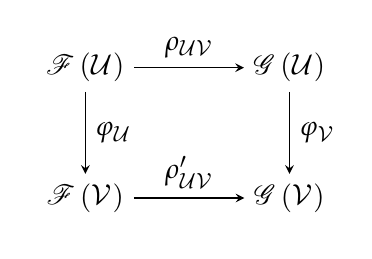
\begin{tikzpicture}
	\matrix (m) [matrix of math nodes,row sep=3em,column sep=4em,minimum width=2em]
	{
\mathscr F\left( \sU\right)   & \mathscr G\left( \sU\right)\\
\mathscr F\left( \sV\right)    & \mathscr G\left( \sV\right)\\
	};
	\path[-stealth]
	(m-1-1) edge node [above] {$\rho_{\sU\sV}$} (m-1-2)
	(m-1-1) edge node [right] {$\varphi_\sU$} (m-2-1)
	(m-1-2) edge node [right] {$\varphi_\sV$} (m-2-2)
	(m-2-1) edge node [above] {$\rho'_{\sU\sV}$} (m-2-2);
\end{tikzpicture}
\\
is commutative, where $\rho_{\sU\sV}$ and $\rho'_{\sU\sV}$ are the restriction maps in $\mathscr F$  and $\mathscr G$. If $\mathscr F$  and $\mathscr G$ are sheaves on $\sX$, we use the same definition for a morphism 
of sheaves. An isomorphism is a morphism  which has a two-sided inverse. 
\end{definition}

\begin{prdf}\label{sheaf_prdf}\cite{hartshorne:ag}
	Given a presheaf $\mathscr F$, there is a sheaf  $\mathscr F^+$ and a morphism $\th: \mathscr F \to \mathscr F^+$, with the property that for any sheaf  $\mathscr G$, and any morphism $\varphi: \mathscr F \to \mathscr G$, there is a unique morphism $\psi:\mathscr F^+\to \mathscr G$ such that $\varphi = \psi \circ \th$. Furthermore the pair $\left(\mathscr F^+, \th\right)$ is unique up to unique isomorphism. $\mathscr F^+$ is called the $\mathrm{sheaf~associated}$ to the presheaf $\mathscr F$. 
\end{prdf}

\begin{empt}\label{sheaf_empt}
	Following text is the citation of the proof of \ref{sheaf_prdf} (cf. \cite{hartshorne:ag}). For any open set $\sU$, let $\mathscr F^+\left(\sU\right)$ be set of functions $s$ from $\sU$ to the union $\bigcup_{x \in \sU}  \mathscr F_x$ of stalks of $\mathscr F$ over points of $\sU$, such that
	\begin{itemize}
		\item [(1)] for each $x \in \sU$, $s\left(x\right)\in \mathscr F_x$, and
		\item[(2)] for each $x \in \sU$, there is a neighbourhood $\sV$ of $x$ contained in $\sU$ and an element $t \in \mathscr F\left(\sV\right)$, such that for all $y \in \sV$ the stalk (germ) $t_y$ of $t$ at $y$ is equal to $s\left(y\right)$.
	\end{itemize}
\end{empt}

\begin{exercise}\label{sheaf_etale_exer}\cite{hartshorne:ag}
	%1.13. 
	\textit{
		\'Espace Etal\'e of a Presheaf}. %(This exercise is included only to establish the connection between our definition of a sheaf and another definition often found in the literature. See for example Godement [1, Ch. II,  1.2].)
	Given a presheaf $\mathscr F$ on $\sX$, we define a topological space $\mathrm{Sp\acute{e}}\left(\mathscr F \right)$ , called the \textit{
		\'espace etal\'e} of a presheaf of $\mathscr F$ as 
	follows. As a set, $\mathrm{Sp\acute{e}}\left(\mathscr F \right)= \bigcup_{x\in\sX} \mathscr F_x$. We define a projection map $p: \mathscr \mathrm{Sp\acute{e}}\left(\mathscr F \right)$
	by sending $s_x\in \mathscr F_x$ to $x$. For each open set $\sU\subset\sX$ and each section $s\in \mathscr F\left(\sU \right)$  we 
	obtain a map: $\overline{s}: \sU \to  \mathrm{Sp\acute{e}}\left(\mathscr F \right)$ by sending $x \mapsto s_x$, its germ at $x$. This map has the property that 
	$p\circ \overline{s}= \Id_\sX$, in other words, it is a "section" of $p$ over $\sU$. We now 
	make $\mathrm{Sp\acute{e}}\left(\mathscr F \right)$ into a topological space by giving it the strongest topology such that 
	all the maps $\overline{s}: \sU \to  \mathrm{Sp\acute{e}}\left(\mathscr F \right)$ for all $\sU$ and all $s\in \mathscr F\left(\sU \right)$ , are continuous. Now 	show that the sheaf $\mathscr F^+$ associated to $\mathscr F$ can be described as follows: for any 
	open set $\sU\subset \mathscr F$, $\mathscr F\left(\sU \right)$ is the set of continuous sections of $\mathrm{Sp\acute{e}}\left(\mathscr F \right)$ over $\sU$. In 
	particular, the original presheaf $\mathscr F$ was a sheaf if and only if for each $\sU\subset \sX$,  $\mathscr F\left(\sU \right)$ is 
	equal to the set of all continuous sections of $\mathrm{Sp\acute{e}}\left(\mathscr F \right)$ over $\sU$. 
	
\end{exercise}
	\begin{empt}\label{open_sheaf_empt}
	For any topological space $\sX$ there is a \textit{sheaf of stalks of open sets} $\Om_\sX$ on $\sX$ (cf. \cite{goldblatt:topoi})		such that
	\bean
	\Om_\sX \left(\sU \right)  \bydef  \text{the family of all open subsets of }\sU;\\
	\rho_{\sU \sV}: \Om_\sX\left(\sU \right) \to \Om_\sX\left(\sV \right), \quad \mathcal W \mapsto \mathcal W \cap \sV.
	\eean
\end{empt}
\begin{exercise}\label{sheaf_etale_open_exer}
Let $\mathscr F$  and $\mathscr G$ by presheaves. Prove that any morphism corresponds to a continuous map $\phi:\mathrm{Sp\acute{e}}\left(\mathscr F \right)\to \mathrm{Sp\acute{e}}\left(\mathscr G \right)$ such that
\begin{itemize}
	\item $p_{\mathscr G}= p_{\mathscr F} \circ \phi$ where both $p_{\mathscr F}: \mathrm{Sp\acute{e}}\left(\mathscr F \right)\to \sX$ and  $p_{\mathscr G}: \mathrm{Sp\acute{e}}\left(\mathscr G \right)\to \sX$ are natural projections.
\item For all $x \in \sX$ a restriction $\phi|_{\mathscr F_x}: \mathscr F_x \to \mathscr G_x$ is a homomorphism of Abelian groups, rings, modules, etc.
\end{itemize}
\end{exercise}

\begin{remark}\label{sheaf_rem}
	If $\sV \subset \sX$ is any subset  then  one can define a group $\mathscr F\left(\sV\right)$  which is a group of continuous maps  $\iota :\sV\to \mathrm{Sp\acute{e}}\left(\mathscr F \right)$ such that $p\circ\iota = \Id_\sV$. Denote by  $\mathscr F\left(\sV \right)$ the Abelian group of such maps.
\end{remark}
\begin{empt}
	For any sheaf $\F$ on $\sX$ and open set $\sU \subset \sX$ we let $C^0\left(\sU, \sF \right)$  be the
	collection of all functions (not necessarily continuous) $f: \sU \to \F$ such
	that $\pi\circ f$ is the identity on $\sU$, $\pi \sF \to \sX$ being the canonical projection.
	Such possibly discontinuous sections are called serrations, a terminology
	introduced by Bourgin [10]. That is,
	$$
	C^0\left(\sU, \sF \right) = \prod_{x \in \sU} \F_x
	$$
	Under pointwise operations, this is a group, and the functor $\sU \mapsto 	C^0\left(\sU, \sF \right)$,
	is a conjunctive monopresheaf on $\sX$. Hence this presheaf is a sheaf, which
	will be denoted by 	$\mathscr C^0\left(\sU, \sF \right)$. Note that if $\sX_d$ denotes the point set of $\sX$
	with the discrete topology and if $f : \sX_d \to \sX$ is the canonical map, then
	$\mathscr C^0\left(\sU, \sF \right)\cong ff^*\F$.
\end{empt}
\begin{definition}\label{sheaf_inv_im_defn}\cite{hartshorne:ag}
	Let $f: \sX\to \sY$ be a continuous map of topological spaces. For any sheaf  $\mathscr F$ on $\sX$, we define the \textit{direct image} sheaf  $f_*\mathscr F$ on $\sY$ by $\left(f_*\mathscr F\right)\left(\sV\right)= \mathscr F\left(f^{-1}\left(\sV\right)\right)$ for any open set $\sV \subseteq \sY$. For any sheaf  $\mathscr G$ on $\sY$, we define the \textit{inverse image} sheaf  $f^{-1}\mathscr G$ on $\sX$ be the sheaf  associated to the presheaf  $\sU \mapsto \lim_{\sV \supseteq f\left(\sU\right)} \mathscr G\left(\sV\right)$, where $\sU$ is any open set in $\sX$, and the limit is taken over  all open sets $\sV$ of $\sV$ containing $f\left(\sU\right)$.
\end{definition}
\begin{remark}\label{sheaf_inv_im_rem} If $f: \sX\to \sY$ be a continuous map  
 of topological spaces and sheaves $\mathscr F$ and $\mathscr G$ on $\sX$ and $\sY$ then there are natural morphisms of sheaves $f^{-1}f_* \mathscr F \to \mathscr F$ and $\mathscr G \to f_*f^{-1}\mathscr G$. See \cite{bredon:sheaf} for details.
\end{remark}
%\begin{remark}\label{geometric_morphism_rem}\cite{johnstone:topos}
%1.17
%	If $f : \sX \to \sY$ is a continuous map then a pair  of functors $f_*$ and $f^*$ rise a geometric morphism (cf. Definition \ref{geom_mor_defn}) $\mathbf{Sh}\left(\sY\right)\to \mathbf{Sh}\left(\sX\right)$ between categories of sheaves. 
%\end{remark}

\begin{definition}\label{sub_sheaf_defn}\cite{hartshorne:ag}
	A \textit{subsheaf}  of a sheaf $\mathscr F$ is a sheaf $\mathscr F'$ such that for every open set 
	$\sU \subset \sX$, $\quad \mathscr F'\left(\sU \right)$  is a subgroup of $\mathscr F\left(\sU \right)$, and the restriction maps of the 
	sheaf $\mathscr F'$ are induced by those of $\mathscr F$. It follows that for any point $P$, the 
	stalk $\mathscr F'_P$ is a subgroup of $\mathscr F_P$. 
	%If (p: & -> ^ is a morphism of sheaves, we define the fce/w/ of (p, denoted ker cp, to be the presheaf kernel of cp (which is a sheaf). Thus ker cp is a subsheaf of .^. We say that a morphism of sheaves cp:^ -> (^ is injeetive if ker (p = 0. Thus <p is injeetive if and only if the induced map cp{U)\^(U) -> ^(G) is 	injeetive for every open set of X. 	If cp\ 3F -> ^ is a morphism of sheaves, we define the zm^ of cp, 	denoted im cp, to be the sheaf associated to the presheaf image of cp. By 	the universal property of the sheaf associated to a presheaf, there is a 	natural map im cp -> rS. In fact this map is injeetive (see Ex. 1.4), and thus 	im cp can be identified with a subsheaf of f&. 	We say that a morphism cp\, -> ^ of sheaves is sitrjective if im cp = f^. 	We say that a sequence . . .  > ^l~"] - > .Wl ^> ,l^x -> . . . of sheaves 	and morphisms is ^xacr if at each stage ker <p' = im cpl ~ l. Thus a sequence
		
	\end{definition}
	

\begin{definition}\label{sheaf_hom_defn}\cite{hartshorne:ag}
	Let $\mathscr F$, $\mathscr G$ be sheaves of Abelian  groups  on $\sX$. For any open set $\sU \subseteq \sX$ the set of morphisms
	 $\Hom\left(\left.\mathscr F\right|_{\sU}, \left.\mathscr G\right|_{\sU}\right)$ has the natural structure of Abelian group. 
	It is a sheaf  (cf. \cite{hartshorne:ag}). It is called the \textit{sheaf of local morphisms} of $\mathscr F\to \mathscr G$, "sheaf hom" for short, and is denoted by $\mathscr Hom \left(\mathscr F, \mathscr G\right)$.
\end{definition}

\begin{definition}\label{sheaf_ringed_space_defn}\cite{hartshorne:ag}
	A \textit{ringed space} is a pair $\left(\sX, \mathcal O_\sX \right)$  consisting of a topological space 
	$\sX$ and a sheaf of rings $\mathcal O_\sX$  on $\sX$.
	% A morphism of ringed spaces from (X,CX) to (Y,GY) is a pair (./,/#) of a continuous map f:X-+ Y and a map f# :(ry -> fJ9x of sheaves of rings on Y. The ringed space (X,x) is a locally ringed space if for each point P e X, the stalk ([x P is a local ring. A morphism of locally ringed spaces is a morphism (/,/#) of ringed spaces, such that for each point P e X, the induced map (see below) of local rings fp :Cyj(P) -+ x,p ls a lcal homomorphism of local rings. We explain this last condition. First of all, given a point P e X, the morphism of sheaves f*:((Y -+ l\fix induces a homomorphism of rings CY(V) -> x(f~ { V), for every open set V in Y. As V ranges over  all open neighbor- 	hoods of /(P), f~l(V) ranges over   a subset of the neighbourhoods of P. 	Taking direct limits, we obtain a map 	&YJ{P) = \jmCY(V)^\jme>'x(f-1V), 		72 
			
		\end{definition}
		\begin{example} \label{sheaf_ringed_space_exm}
			One has a following ringed spaces (cf.Definition \ref{sheaf_ringed_space_exm})
			\begin{enumerate}
				\item [(i)] If $\sX$ is topological space and a sheaf   $\mathscr C_\sX$ associated with a presheaf
				$$
				\sU \mapsto C_0\left( \sU\right) 
				$$
				then $\left(\sX, \mathscr C_\sX \right)$ is a ringed space.
				\item [(ii)]If $M$ is smooth manifold and a sheaf   $\mathscr C^\infty_M$ associated with a presheaf
				$$
				\sU \mapsto \Coo\left( \sU\right) 
				$$
				then $\left(M, \mathscr C^\infty_\sX \right)$ is a ringed space.
			\end{enumerate}
		\end{example}
		
		\begin{definition}\label{sheaf_of_modules_den}\cite{hartshorne:ag}
			Let $\left(\sX, \mathcal O_\sX \right)$  be a ringed space. A \textit{sheaf  of $ \mathcal O_\sX $-modules} 
			(or simply an $\mathcal O_\sX$ -\textit{module}) is a sheaf  $\mathscr F$ on $\sX$, such that for each open set 
			$\sU\subset\sX$, the group 
			$\mathscr F\left(\sU \right)$ is an $\mathcal O_\sX$-module, and for each inclusion of 
			open sets $\sV \subset\sU$, the restriction homomorphism $\mathscr F\left(\sU \right) \to \mathscr F\left(\sV \right)$  is compatible with the module structures via the ring homomorphism $\mathcal O_\sX\left(\sU \right) \to \mathcal O_\sX \left(\sV \right)$.
			%	(9X(V). A morphism #"  > ^ of sheaves of $x-modules is a morphism of 
			%	sheaves, such that for each open set U ^ X, the map <F(U) -> ^(7) is a 
			%	homomorphism of $x(L/)-modules. 	Note that the kernel, cokernel, and image of a morphism of 6rx-modules 	is again an Gx-modu\e. If ^'ls a subsheaf  \ref{top_x_sheaf_defn} of (^'x-modules of an (9x-modu\e 	#", then the quotient sheaf \ref{top_x_sheaf_defn} gFj^F' is an #x-module. Any direct sum, 	direct product, direct limit, or inverse limit of $x-modules is an $x-module. 	If J^ and ^ are two $x-modules, we denote the group of morphisms from 	^ to ^ by Hom^^,^), or sometimes Homx(J^) or Hom( J^) if no 	confusion can arise. A sequence of $x-modules and morphisms is exact 	if it is exact as a sequence of sheaves of abelian groups. 	If U is an open subset of X, and if J^ is an $x-module, then tF\v is an 	(9x\v-modu\e. If 3F and ^ are two ^x-modules, the presheaf  \ref{top_x_sheaf_defn} 	is a sheaf, which we call the sheaf  \ref{top_x_sheaf_defn} Worn (Ex. 1.15), and denote by 	.^bm^l^). It is also an $x-module. 
		\end{definition}
		
	
		
		
		
	
\section{Flasque (flabby) and soft  sheaves}
\begin{definition}\label{sheaf_flasque}\cite{hartshorne:ag}
	A sheaf  $\mathscr F$ on a topological space is \textit{flasque} or \textit{flabby} if for every inclusion $\sV \subseteq \sU$ of open sets, the restriction map $\mathscr F\left(\sU \right)\to\mathscr F\left(\sV \right)$ is surjective. 
\end{definition}
Recall that for $s \in \mathscr{F}\left(\sX \right)$, 
\be\label{sheaf_supp_eqn}
\supp s= \left\{\left.x \in \sX \right|s\left(x \right)\neq 0  \right\}
\ee
 denotes the \textit{support} of the section $s$.
\begin{definition}\label{phi_supp_defn}\cite{godement:sheaf}.
	Let $\sX$ be a topological space. A \textit{family of supports} on $\sX$ is a family $\Phi$ of closed
	subsets of $\sX$  such that:
	\begin{enumerate}
		\item a closed subset of a member of $\Phi$ is a member of $\Phi$;
		\item $\Phi$ is closed under finite unions.
	\end{enumerate}
	
	$\Phi$  is said to be a  \textit{paracompactifying} family of supports if in addition:
	\begin{enumerate}
		\item  each element of $\Phi$ is paracompact;
		\item each element of $\Phi$ has a (closed) neighbourhood which is in $\Phi$.
	\end{enumerate}
\end{definition}\label{sheaf_soft_defn}
The family of all compact subsets of $\sX$ is denoted by $c$.
\begin{definition}\label{soft_sheaf_defn}\cite{bredon:sheaf}
	A sheaf  $\mathscr{F}$ on $\sX$ is called $\Phi$-\textit{soft} if the restriction map	$\mathscr{F}\left(\sX \right) \to  \mathscr{F}\left(K \right)$  is surjective for all $K \in \Phi$. If $\Phi$ is a set of all closed sets  then $\Phi$ is simply
	called \textit{soft}. If $\Phi= c$ is a set of all compact  sets  then $\mathscr{F}$ is called $c$-\textit{soft}.
\end{definition}
\begin{theorem}\label{sheaf_soft_m_thm}\cite{bredon:sheaf}
 Let $\left(\sX, \mathcal O_\sX \right)$ be a ringed space (cf. Definition \ref{sheaf_ringed_space_defn}), and let $\mathscr F$ be an $\mathcal O_\sX$-module (cf. Definition \ref{sheaf_of_modules_den}). Suppose that the space $\sX$ is paracompact and $\Phi$ is a {paracompactifying} family of supports(cf. Definition \ref{phi_supp_defn}). If the sheaf $\mathcal O_\sX$ is $\Phi$-soft (cf. Definition \ref{soft_sheaf_defn}) then  $\mathscr F$ is also $\Phi$-soft.
\end{theorem}


%\begin{theorem}\label{sheaf_homototy_thm} Any two properly homotopic maps (with respect to $\Phi$ and $\Psi$)
%	of a space $X$  into a space $Y$ induce identical homomorphisms
%	$$
%	H^*_\Psi(Y;G)\to  H^*_\Phi(X;G),
%	$$
%	where $G$ is any constant coefficient group.
	
%\end{theorem}
%Note the special cases:
%\begin{itemize}
%	\item [(a)]  $\Phi = cld = \Psi$. In this case, "properly homotopic" is the same as
%	"homotopic."
%	\item [(b)] $X, Y$ locally compact Hausdorff, $\Phi = c = \Psi$.
%\end{itemize}
%There is a theorem in Bredon's book (page 80).
%\begin{theorem} Any two properly homotopic maps (with respect to $\Phi$ and $\Psi$)
%	of a space $X$  into a space $Y$ induce identical homomorphisms
%	$
%	H^*_\Psi(Y;G)\to  H^*_\Phi(X;G),
%	$
%	where $G$ is any constant coefficient group.
	
%\end{theorem}


%For a presheaf $\mathscr{P}$  on $\sX$ we put  $\mathscr{P}_\Phi\left(\sX \right) = \left\{\left.s\in \mathscr{P}\left( \sX\right)\right| \left|s\right| \in \Phi \right\}$.
\begin{lemma}\label{sheaf_soft_neighbourhood_lem}\cite{godement:sheaf,torsten:sheaves}
	Let $\sX$ be a paracompact space, $\mathscr{F}$ a sheaf on $\sX$. Then $\mathscr{F}$ is soft if and only if every point $x \in \sX$ has a closed neighbourhood $\overline{   \mathcal U }$ such that $\left.\mathscr{F}\right|_{\overline{   \mathcal U }}$ is soft.
\end{lemma}

%\begin{theorem}\cite{bredon:sheaf}
	%	6.2.\\
%	Theorem. Let $\mathscr P$ be a presheaf  DEFN \ref{top_x_sheaf_defn} on $\sX$ that is conjunctive for coverings	of $\sX$ and $\mathscr P^+$ be the sheaf \ref{top_x_sheaf_defn} generated by $\mathscr P$. Then for any paracompactifying 	family $\Phi$ of supports on $\sX$, the sequence
%	$$
%	0 \to \mathscr P_0\left( \right) \to  \mathscr{P}_\Phi\left(\sX \right) \xrightarrow{\th}\Ga_\Phi\left(\mathscr{P}^+ \right) 
%	$$
%	is exact.
%\end{theorem}
%\begin{theorem}\label{sheaf_neigh_thm}\cite{godement:sheaf}
	%	3.3.1\\
%	Let $\mathscr{F}$ be a sheaf  of set over the space $\sX$, $\mathcal S$ is a subset of $\sX$ and $s$ is a section of the sheaf  $\mathscr{F}$ over $\mathcal S$. If $\mathcal S$ allow !!! ADMIT !!!s a fundamental system of paracompact neighbourhoods then $s$ can be extended to a neighbourhood of $\mathcal S$ in $\sX$. 
%\end{theorem}
\begin{theorem}\label{soft_french_thm}
%Thorme 3.4.1-   
Soit $\mathscr F$ un faisceau surun espace $\sX$ paracompact. Supposons que tout point de $\sX$ poss de un  voisinage $\sU$ v rifiant la condition suivante : toute section de $\mathscr F$au-dessus d'un sous-ensemble ferm  de $\sX$ contenu dans $\sU$, se prolonge   $\sU$. Alors $\mathscr F$ est mou.
\end{theorem}
Following text is an English translation of the above theorem
\begin{theorem}\label{soft_e_thm}
	Let  $\mathscr{ F}$ be a sheaf on  a paracompact space $\sX$. Suppose that for any $x \in\sX$ there is a neighbourhood  $\sU$ which satisfies to the following condition; every section of $\mathscr{ F}$ over closed subset  $\sY\subset \sX$ such that $\sY\subset \sU$ can be extended up to $\sU$. Then the sheaf $\mathscr{ F}$ is soft.
\end{theorem}
%\begin{thm}\cite{godement:sheaf}
%Thorme 3-7-2.   
%Soit $\mathscr{ A}$ un faisceau d'anneaux avec unit  sur un espace paracompact $\sX$. Pour que $\mathscr{ A}$ soit mou, il faut et il suffit que tout point de $\sX$ poss de un  voisinage $\sU$ tel que, 	 tant donn s des ferm  disjoints $S,T \subset \sU$, il existe une section de $\mathscr{ A}$ au-dessus de $\sU$,  gale   1 sur $S$ et   0 sur $T$.
%\end{thm}
%Following text is an English translation of the above theorem.
%\begin{theorem}\label{sheaf_a_soft_thm}
%Let $\mathscr{ A}$ be a sheaf of unital algebras on a paracompact apace $\sX$. The sheaf $\mathscr{ A}$ is soft if and only if any $x\in\sX$ have a neighbourhood $\sU$ such that for any closed sets $S, T\subset \sU$ one has
%\bean
%S\cap T = \emptyset \quad \Rightarrow \quad \exists s \in \mathscr{ A}\left( \sU\right) \quad s|_S = 1\quad \mathrm{AND} \quad \quad s|_T = 0.
%\eean
%\end{theorem}

%\begin{proposition}\label{flabby_soft_prop}\cite{bredon:sheaf}
	%	9.22. Proposition. \\
%	If $\sU$ is a compact relatively Hausdorff subspace of $\sX$,
%	then $\left.\mathscr{F}\right|_{\sU} $ is soft for any flabby sheaf  $\mathscr{F}$ on $\sX$.
%\end{proposition}
	\begin{definition}\label{sheaf_flabby_defn}\cite{hartshorne:ag}
	A sheaf  $\mathscr F$ on a topological space is \textit{flasque} or \textit{flabby} if for every inclusion $\sV \subseteq \sU$ of open sets, the restriction map $\mathscr F\left(\sU \right)\to\mathscr F\left(\sV \right)$ is surjective. 
\end{definition}
\section{Sheaves over   non Hausdorff spaces}\label{sheaves_nh_sec}
\begin{empt}\label{nh_csoft_empt}\cite{cra_moe:nhaus}
	Here we assume that the space $\sX$ has an open cover   by subsets $\sU \subset \sX$ which are each paracompact, Hausdorff, locally compact and of cohomological dimension bounded a number $d$ (depending  on $\sX$ but not $\sU$).	
\end{empt}

\begin{definition}\label{nh_csoft_defn}\cite{cra_moe:nhaus}
	Let $\sX$ be a space satisfying the assumptions of \ref{nh_csoft_empt}. An Abelian sheaf $\mathscr{F}$ is said to be $c$-!!!\textit{soft} if for any open $\sU \subset \sX$ its restriction $\left.\mathscr{F}\right|_{\sU}$ is a soft on $\sU$ in the usual sense. By the same proprety of for Hausdorff space, it follows that softness is a local property, i.e. a sheaf   $\mathscr{F}$ is soft if and only if there is an open cover   $\sX= \cup \sU_\a$  such that $\left.\mathscr{F}\right|_{\sU_\a}$ is a soft sheaf  on $\sU$.
\end{definition}
\begin{definition}\label{nh_csoft_gc_defn}\cite{cra_moe:nhaus}
	Let $\mathscr{F}$ be a soft sheaf  and let $\mathscr{F}'$  be its Godement resolution (i.e. $\mathscr{F}'= \Ga\left(\sU_{\text{distr}}, \mathscr{F} \right)$ is the set of all (not necessary continuous) sections for any open $\sU \subset \sX$). For any Hausdorff open set $\mathcal W$, let $\Ga_c\left(\mathcal W, \mathscr{F} \right)$ be the usual set of compactly supported sections. If $\mathcal W \subset \sU$, there is an evident homomorphism "extension by 0" 
	\be\label{sheaf_inc_eqn}
	\Ga_c\left(\mathcal W, \mathscr{F} \right) \hookto \Ga_c\left(\mathcal U, \mathscr{F} \right)\subset \Ga_c\left(\mathcal U, \mathscr{F}' \right).
	\ee
 For any (not necessary Hausdorff) open set $\sU \subset \sX$ we define $\Ga_c \left(\sU, \mathscr{F} \right)$ to be the image of the map:
	$$
	\bigoplus_{\mathcal W} \Ga_c\left(\mathcal W, \mathscr{F}' \right) \hookto \Ga\left(\mathcal U, \mathscr{F}' \right),
	$$ 
	where $\mathcal W$ ranges over  all open subsets $\mathcal W \subset \mathcal U$. %An alternative definition follows by choosing open cover   in Propositions \ref{nh_csoft_gc_prop} below.
\end{definition}
\begin{proposition}\label{nh_csoft_gc_lem}
	Let  $\mathscr{F}$ be a soft sheaf. For any open cover   $\sU = \cup \mathcal W_\a$ where each $\mathcal W_\a$ is Hausdorff the sequence $\oplus_\a \Ga_c\left(\mathcal W_\a,  \mathscr{F}\right) \to \Ga_c\left(\mathcal U,  \mathscr{F}\right)\to 0$ is exact.  
\end{proposition}
	\subsection{Derived functors}

\begin{definition}
	An \textit{Abelian category} is a category $\mathfrak{A}$, such that: $\Hom\left(A, B \right)$ has a structure of an Abelian group for each objects $A,~ B$ of $\mathfrak{A}$, and the composition law is linear; finite direct sums exist; every morphism has a kernel 
	and a cokernel; every monomorphism is the kernel of its cokernel, every 
	epimorphism is the cokernel of its kernel; and finally, every morphism 
	can be factored into an epimorphism followed by a monomorphism. 
\end{definition}
\begin{empt}
	A \textit{complex} $A^\bullet$ in an 
	Abelian category  $\mathfrak{A}$ is a collection of objects $A^n$, $n \in \Z$, and morphisms 
	$d^n : A^n \to A^{n + 1}$, such that $d^{n+1} \circ d^n = 0$ for all $n$. If the objects $A^n$ are specified 
	only in a certain range, e.g., $n \ge 0$, then we set $A^n = 0$ for all other $n$. A 
	morphism of complexes, $f: A^\bullet \to B^\bullet$ is a set of morphisms $f^n : A^n \to B^n$ for 
	each $n$, which commute with the coboundary maps $d^n$. 
	The $n$th cohomology object $h^n\left( A^\bullet\right)$  of the complex $A^\bullet$  is defined to be
	\be
	h^n\left( A^\bullet\right)\bydef \ker d^n / \im d^n.
	\ee 
	If $f : A^\bullet \to B^\bullet$ is a morphism of complexes, then $f$ induces a natural map $h^n\left(f \right) : h^n\left(A^\bullet \right)\to h^n\left(B^\bullet \right)$. If $0 \to A^\bullet \to B^\bullet \to C^\bullet$ 
	is a short 
	exact sequence of complexes, then there are natural maps $\dl^n : h^n \left( C^\bullet\right) \to h^n \left( A^\bullet\right)$ 
	giving rise to a long exact sequence 
	\bean 
	\dots 	 h^n \left( A^\bullet\right) \to h^n \left( B^\bullet\right)\to h^n \left( C^\bullet\right)\xrightarrow{\dl^n} h^{n+1} \left( A^\bullet\right)\to \dots.
	\eean
	Two morphisms of complexes $f, g : A^\bullet\to B^\bullet$ are \textit{homotopic} (written $f \sim g$) 
	if there is a collection of morphisms $k^n : A^n \to B^{n-1}$ for each $n$ (which need 
	not commute with the $d^n$) such that $f - g = d k - k d$. The collection of morphisms, $\left\{k^n\right\}$ is called a \textit{homotopy operator}. If $f \sim g$, then $f$ and $g$ induce 
	the \textit{same} morphism  $h^n \left( A^\bullet\right)\to  h^n \left( B^\bullet\right)$ on the cohomology objects, for each $n$. 
\end{empt}
\begin{definition}
	A covariant functor $F:\mathfrak A \to \mathfrak B$ from one Abelian category to another is 
	\textit{additive} if for any two objects $A, A'$ in $\mathfrak A$, the induced map $\Hom(A,A') \to  
	Hom(FA,FA')$ is a homomorphism of Abelian groups. $F$ is \textit{left exact} if it is 
	additive and for every short exact sequence 
	$$
	0 \to A' \to A \to A'' \to 0
	$$
	in $\mathfrak A$, the sequence 
	$$
	0 \to FA' \to FA \to FA'' 
	$$
	is exact in $\mathfrak B$. If we can write a 0 on the right instead of the left, we say $F$ is 
	\textit{right exact}. If it is both left and right exact, we say it is \textit{exact}. If only the 
	middle part $FA' \to FA \to FA''$ is exact, we say F is \textit{exact in the middle}. 
	For a contravariant functor we make analogous definitions. For example, 
	$F:\mathfrak A \to \mathfrak B$ is \textit{left exact} if it is additive, and for every short exact sequence as 
	above, the sequence 
	$$
	0 \to FA'' \to FA \to FA' 
	$$
	is exact in $\mathfrak B$. 
	
\end{definition}	


\begin{definition}
	An object $I$ of $\mathfrak  A$ is 
	\textit{injective} if the functor $\Hom\left(\cdot, I\right)$ is exact. An \textit{injective resolution} of an object 
	$A$ of $\mathfrak  A$ is a complex $I^\bullet$, defined in degrees i  0, together with a morphism 
	$\eps A \to I^0$, such that $I^n$ is an injective object of $\mathfrak  A$ for each $n \ge 0$, and such 
	that the sequence 
	\bean
	0\to A \xrightarrow{\eps} I^0 \to I^1 \to \dots
	\eean
	is exact. 
\end{definition}
\begin{definition}
	If every object of $\mathfrak A$ is isomorphic to a subobject of an injective object of 
	$\mathfrak A$, then we say $\mathfrak A$ \textit{has enough injectives}.
\end{definition}
\begin{remark}
	If $\mathfrak A$ has enough injectives, then every 
	object has an injective resolution. Furthermore, a well-known lemma states 
	that any two injective resolutions are homotopy equivalent. 
\end{remark}
\begin{definition}
	let $\mathfrak A$ be an Abelian category with enough injectives, and let $F: \mathfrak A\to\mathfrak B$ 
	be a covariant left exact functor. Then we construct the \textit{right derived functors} 
	$R^nF$, $i \ge 0$, of $F$ as follows. For each object $A$ of $\mathfrak A$, choose once and for all 
	an injective resolution $I^\bullet$ of $A$. Then we define 
	\be
	R^nF\left( A\right) \bydef h^n\left(F\left( I^\bullet\right)  \right) .
	\ee
\end{definition}

\begin{definition}DIMCA !!!
	Let $\mathscr A$
	be an Abelian category and 
	$K\left(\mathscr A \right)$
	its category of chain complexes modulo chain homotopy (the �homotopy category of chain complexes�).
	
	Equip 
	$K\left(\mathscr A \right)$
	with the structure of a homotopical category by declaring the weak equivalences to be the \textit{quasi-isomorphisms}: those morphisms 
	$f: V\to W$
	which induce isomorphisms in (co)homology $H(F) \to H\left(W \right)$. The \textit{derived category}
	$D\left( \mathscr A\right)$
	is the homotopy category of 
	with respect to these weak equivalences
	is the homotopy category of $\mathscr A$
	with respect to these weak equivalences.
\end{definition}

\begin{theorem}\label{derived_finctor_thm}\cite{hartshorne:ag}
	%			Theorem 1.1 A. 
	Let $\mathfrak A$ be an Abelian category with enough injectives, and let 
	$F: \mathfrak A \to  \mathfrak B$ be a covariant left exact functor to another Abelian category $\mathfrak B$. 
	Then 
	\begin{enumerate}
		\item [(a)] For each $n \ge 0$, $R^nF$ as defined above is an additive functor from  $\mathfrak A$ 
		to $\mathfrak B$. Furthermore, it is independent (up to natural isomorphism of functors) 
		of the choices of injective resolutions made.
		\item[(b)] There is a natural isomorphism $F \cong R^0F$.
		\item[(c)] For each short exact sequence $0 \to A'\to A \to A'' \to 0$ and for each 
		$n \ge 0$ there is a natural morphism $\delta^n: R^nF\left(A''\right)\to R^{n +1}F\left(A''\right)$, such that we 
		obtain a long exact sequence 
		$$
		\dots \to R^nF\left(   A'\right) \to R^nF\left(   A\right) \to R^nF\left(   A''\right) \xrightarrow{\delta^n} R^{n+1}F\left(   A'\right) \to  R^{n+1}F\left(   A\right) \to \dots.
		$$
		\item[(d)] Given a morphism of the exact sequence of (c) to another $0\to B'\to B \to B''\to 0$, the $\delta$'s give commutative diagram 
		\newline
		\begin{tikzcd}
			R^{n}F\left(A'' \right) \arrow[d]\arrow[r, "\dl^n"]
			&  R^{n+1}F\left(A'' \right) \arrow[d]\\
			R^{n}F\left(B'' \right)\arrow[r, "\dl^n"]	&  R^{n+1}F\left(B' \right)
		\end{tikzcd}
		\item[(e)] For each injective object $I$ of $\mathfrak A$, and for each $n \ge 0$, we have $R^nF\left(I\right)= 0$.
	\end{enumerate}
\end{theorem}
\begin{definition}\label{acyc_defn}\cite{hartshorne:ag}
	With 	$F: \mathfrak A \to  \mathfrak B$  as in the theorem \ref{derived_finctor_thm}, an object $J$ of $\mathfrak A$ is \textit{acyclic} for 
	$F$ if $R^pF = 0$ for all $p > 0$. 
\end{definition}
\begin{proposition}\label{acyc_prop}\cite{hartshorne:ag}
	%Proposition 1.2A. 
	With 	$F: \mathfrak A \to  \mathfrak B$  as in the theorem \ref{derived_finctor_thm}, suppose there is an exact 
	sequence 
	$$
	0 \to A \xrightarrow{\dl_0} J^0 \xrightarrow{\dl_1}J^1 \to \dots
	$$
	where each $J^p$ is acyclic for $F$,  $p\ge 0$. (We say $J^\bullet$ is an $F$-\textit{acyclic resolution}
	of $A$.) Then for each $p \ge 0$ there is a natural isomorphism $R^p\left( F\left(A \right) \right) = h^p\left( F\left( J^\bullet\right) \right)$
	where 
	\be\label{derivation_eqn}
	\begin{split}
		h^p\left( F\left( J^\bullet\right) \right)\bydef\begin{cases}
			\ker F\left( \dl^0 \right) & p = 0\\
			\ker~ F\left(  \dl_{p} \right) / \im~ F\left(  \dl_{p-1}\right)   & p > 0
		\end{cases}
	\end{split}
	\ee
\end{proposition}

\begin{definition}\cite{hartshorne:ag}
	Let $\mathfrak  A$ and $\mathfrak  B$ be Abelian categories. A (\textit{covariant}) $\dl$-\textit{functor} from 
	$\mathfrak  A$ to $\mathfrak  B$ is a collection of functors $T\bydef \left\{T^n\right\}_{n \ge 0}$, together with a morphism $\dl^n: T^n(A'') \to  T^{n + 1}(A')$ for each short exact sequence $0 \to A'\to A \to A'' \to 0$, 
	and each $n \ge 0$, such that: 
	\begin{enumerate}
		\item[(a)]
		
		For each short exact sequence as above, there is a long exact sequence
		\bean
		0 \to  T^0\left(   A'\right) \to T^0\left(   A\right) \to T^0\left(   A''\right) \xrightarrow{\delta^0} T^{1}\left(   A'\right) \to \dots \\
		\dots \to  T^n\left(   A\right) \to T^n\left(   A''\right) \xrightarrow{\delta^n} T^{n+1}\left(   A'\right) \to  T^{n+1}\left(   A\right) \to \dots;
		\eean 
		\item[(b)] for each morphism of one short exact sequence (as above) into another 
		$0 \to B'\to B \to BA'' \to 0$, the $\dl$'s give a commutative diagram 
		\newline
		\begin{tikzcd}
			T^n\left(A'' \right) \arrow[d]\arrow[r, "\dl^n"]
			&  T^{n+1}\left(A'' \right) \arrow[d]\\
			T^{n}F\left(B'' \right)\arrow[r, "\dl^n"]	&  T^{n+1}\left(B' \right)
		\end{tikzcd}
	\end{enumerate}
\end{definition}
\begin{definition}
	The $\dl$ functor $T\bydef \left\{T^n\right\}_{n \ge 0}: \mathfrak A \to \mathfrak B$, is said to be \textit{universal} if, given 
	any other $\dl$-functor $T'\bydef \left\{T'^n\right\}_{n \ge 0}: \mathfrak A \to \mathfrak B$, and given any morphism of 
	functors $f^0: T^0 \to T'^0$, there exists a unique sequence of morphisms 
	$f^n: T^n \to T'^n$ for each $n \ge 0$, starting with the given $f^0$, which commute 
	with the $\dl^n$ for each short exact sequence. 
\end{definition}
\begin{theorem}\label{uni_delta_thm}
	Assume that $\mathfrak  A$ has enough injectives. Then for any left exact 
	functor $F:\mathfrak  A\to\mathfrak  B$, the derived functors $\left\{R^nF\right\}_{n \ge 0}$ form a universal $\dl$-functor with $F = R^0F$. Conversely, if $T \bydef \left\{T^n\right\}_{n \ge 0}$ is any universal $\dl$-functor, 
	then $T^0$ is left exact, and the $T^n$ are isomorphic to $R^n T^0$ for each $n \ge 0$.
\end{theorem}
\subsection{Cohomology}\label{grothendieck_cohomology_section}
\paragraph{}
Here I follow to \cite{milne:lec}. The functor
\bean
\Ga\left(X, \cdot \right) : \mathbf {Ab} \left(\mathbf T \right) \to \mathbf {Ab} ,\\
\mathscr F \mapsto \mathscr F\left(X \right) 
\eean
of global sections is left exact, and we define $H^r\left(X,~ \cdot ~\right)$ to be its $r^{\text{th}}$ right derived functor.  An exact sequence (cf. Definition \ref{exact_sec_defn})
$$
0 \to \mathscr F \to  \mathscr I^0\xrightarrow{\dl^0} \mathscr I^1\xrightarrow{\dl^1} \mathscr I^2 \to ...
$$
is said to be an \textit{injective resolution} if for all $\mathscr I^p$ is an injective object (cf. Definition \ref{injective_object_defn}) of $\mathfrak  A$ for all $p$.
We apply the functor $\Ga\left(X, \cdot \right)$ to obtain a complex
\be\label{complex_eqn}
\Ga\left(X,\ \mathscr I^0  \right) \xrightarrow{\Ga\left( \dl^0 \right)} \Ga\left(X, \mathscr I^1  \right) \xrightarrow{\Ga\left( \dl^1 \right)} \Ga\left(X, \mathscr I^2  \right) \to ... 
\ee
This is no longer exact (in general).
The complex \eqref{complex_eqn}  and the Theorem \ref{derived_finctor_thm} define the $p^{\text{th}}$ cohomology
group 

\be\label{etale_coh_eqn}
\begin{split}
	H^p\left(X, \mathscr F \right)\bydef  R^r\Ga\left(X, \F \right)\begin{cases}
		\ker \Ga\left( \dl^0 \right) & p = 0\\
		\ker~ \Ga\left(  \dl^{p} \right) / \im~ \Ga\left(  \dl^{p-1}\right)   & p > 0
	\end{cases}
\end{split}
\ee
(cf. equation \eqref{derivation_eqn})
The theory of derived functors (cf. Theorem \ref{derived_finctor_thm}) shows:
\begin{enumerate}
	\item [(a)] $H^0\left(X,\ \mathscr F  \right)\cong \Ga\left(X,\ \mathscr F \right)$ for any sheaf $\mathscr F$;
	\item [(b)] if $\mathscr I$ is injective, then $H^r (X,\mathscr I )= 0$ for $r > 0$;
	\item [(c)]  short exact sequence of sheaves
	$0\to \mathscr F' \to \mathscr F \to \mathscr F'' \to 0$	gives rise to a long exact sequence
	\be\label{long_coh_sec_eqn}
	0 \to H^0\left(X, \mathscr F'  \right) \to H^0\left(X, \mathscr F  \right) \to H^0\left(X, \mathscr F''  \right) \to H^1\left(X,\ \mathscr F'  \right) \to ...
	\ee
	and the association of the long exact sequence with the short exact sequence is functional;
\end{enumerate}
Moreover, the functors $H^r\left( X,~ \cdot ~\right)$  are uniquely determined (up to a unique isomorphism)
by the properties (a), (b) and (c).
\begin{proposition}\label{spectral_sequence_prop}\cite{johnstone:topos}
	%8.17 
	Let $\mathscr F \xrightarrow{f} \mathscr E$ be a geometric morphism (cf. Definition \ref{geometric_morphism_defn}) between Grothendieck toposes (cf. Definition \ref{grothendiek_topos_defn}). Then
	\begin{enumerate}		\item [(i)] 
		if $A$ is an Abelian group in $\mathscr E$ then we have a homomorphism $H^q\left(\mathscr E, A \right) \xrightarrow{} H^q \left(\mathscr F, f^*A\right)$ for each $q$ which is functorial in $f$ and natural in $A$.
		\item [(ii)] If $B$ is an Abelian group in $\mathscr F$ then we have a spectral sequence (Leray spectral sequence) $H^p\left(\mathscr E, R^qf_*\left(B \right) \right)\Rightarrow H^{p + q}\left(\mathscr F, B \right)$ which is natural in $B$.
	\end{enumerate}
\end{proposition}
\begin{notation}\label{const_shef_coh_not}
	If  $F$ is an Abelian group and $F_X$ is a {constant presheaf} (cf. Definition \ref{constant_presheaf_defn}) then we use the following notation
	\be\label{const_shef_coh_eqn}
	\forall r\ge 0\quad H^r\left(X, F \right) \bydef H^r\left(X, \mathfrak{Ass} \left( F_X\right)  \right).
	\ee
	where $\mathfrak{Ass}$ means the associated sheaf functor (cf. Definition \ref{associated_sheaf_defn}).
\end{notation}
\subsection{\v{C}ech cohomology}\label{cech_cohomology_sec}
\paragraph*{} Here I follow to \cite{milne:lec}. Let $\mathbf T$ be a site, and let $X$ be an object of $\mathrm{Cat}\left( \mathbf T\right)$. Let $\mathscr U \bydef \left\{U_\iota \to X\right\}_{\iota \in I}$ be  covering of $X$, and let $\mathscr P$ be a presheaf of Abelian groups. Define
\be\label{cech_eqn}
C^r\left( \mathscr U, \mathscr P\right)\bydef \prod_{\left(\iota_0,.... \iota_r\right) \in I^{r+1}} \mathscr P\left(U_{\iota_0,.... \iota_r} \right)\quad \text{where} \quad U_{\iota_0,.... \iota_r} \bydef U_{\iota_0}\times_X...\times_XU_{\iota_r}. 
\ee
For $s \in C^r\left( \mathscr U, \mathscr P\right)$ define $d^rs \in C^{r+1}\left( \mathscr U, \mathscr P\right)$ by the rule
\be\label{cech_differential_eqn}
d^rs_{\iota_0,..., \iota_{r + 1}}\bydef \sum_{j = 0}^{r + 1}\left(-1 \right) \mathrm{res}_j\left(s_{\iota_0,..., \iota_{j-1},\iota_{j+1},..., \iota_{r + 1}} \right)  
\ee
$\mathrm{res}_j$ is the restriction map corresponding to the projection map
$$
U_{\iota_0,..., \iota_{r + 1}}\mapsto U_{\iota_0,..., \iota_{j-1},...,\iota_{j+1},.., \iota_{r + 1}}.
$$
As in the classical case, one verifies by a straightforward calculation that
\be\label{chech_res_eqn}
C^\bullet\left( \mathscr U, \mathscr P\right) \bydef C^0\left( \mathscr U, \mathscr P\right) \to...\to C^r\left( \mathscr U, \mathscr P\right) \xrightarrow{d_r} C^r\left( \mathscr U, \mathscr P\right)\to ...
\ee
is a complex. Define
\be\label{cech_coh_eqn}
\check{H}^r\left( \mathscr U, \mathscr P\right) \bydef H^r\left(C^\bullet\left( \mathscr U, \mathscr P\right)   \right)= \begin{cases}
	\ker d_0 & r = 0\\
	\ker d_r / \im d_{r-1} & r > 0
\end{cases}. 
\ee
It is called the $r^{\text{th}}$ \textit{\v{C}ech cohomology group} of $\mathscr P$ relative to the covering $\mathscr U$.
Note that
$$
\check{H}^0\left( \mathscr U, \mathscr P\right)= \ker\left(\prod \mathscr P_\iota \rightrightarrows \prod \mathscr P_{\iota,j} \right) 
$$
Therefore, for a sheaf $\mathscr F$ one has
$$
\check{H}^0\left( \mathscr U, \mathscr F\right)=\Ga\left( \mathscr U, \mathscr F\right).
$$
A second covering $\mathscr V \bydef \left\{V_j\to X \right\}_{j \in J}$ of $X$ is called a \textit{refinement} of $\mathscr U$ if there is a
map $\tau : J\to I$ such that $V_j \to X$ factors through $U_{\tau_j}\to X$ for all $j \in J$ . The choice of
a $\tau$ and $X$-morphisms $\varphi_{j}: V_j \to U_{\tau_j}$ for each $j$ determines a map of complexes
\be\label{cech_refi_eqn}
\tau^\bullet: C^\bullet\left( \mathscr U, \mathscr P\right)\to C^\bullet\left( \mathscr V, \mathscr P\right),\\
\left( \tau^r s_{j_0,..., j_{r}} \right) \bydef s_{\tau j_0,..., \tau j_{r}}.
\ee
As in the classical case, one verifies that the map on cohomology groups
$$
\rho \left(\mathscr U, \mathscr V \right): \check{H}^r\left( \mathscr U, \mathscr P\right)\to \check{H}^r \left( \mathscr V, \mathscr P\right)
$$
is independent of all choices. We may pass to the limit over all coverings, and so obtain limits
\be\label{chech_eqn}
\check{H}^r\left(X, \mathscr P\right)\bydef \varinjlim_{\mathscr U}\check{H}^r\left( \mathscr U, \mathscr P\right).
\ee
\begin{defn}\label{cech_defn}\cite{bryl:loop,milne:lec}
	The  \textit{\v{C}ech cohomology groups} are given by equation \eqref{chech_eqn}.
\end{defn}
These groups  have the following properties:
\begin{enumerate}
	\item [(a)] $\check{H}^0\left(X, \mathscr F\right)= \Ga\left( X, \mathscr F\right)$ for any sheaf $\mathscr F$ on $X$;
	\item[(b)] $\check{H}^r\left(X, \mathscr I\right)$, $r > 0$, for all injective sheaves $\mathscr I$
\end{enumerate}
(cf \cite{milne:lec} for details).
\begin{empt}
	For any Abelian group $F$ one can define a constant presheaf $F_X$ of Abelian groups (cf. Definition \ref{constant_presheaf_defn}). 
	We use a following notation
	\be\label{etale_hom_a_eqn}
	\check{H}^r\left(X, F\right)\bydef \check{H}^r\left(X, F_X\right).
	\ee
\end{empt}
\begin{remark}
	% PAGE 
	It is proven in \cite{johnstone:topos} that for any presheaf $\mathscr A$ on the site $\mathbf{T}$ and any $U \in \mathrm{Cat}\left( \mathbf T\right)$ one has
	\be\label{cech_ass_eqn}
	\check{H}^0\left( \sU, \mathscr A\right) = \varinjlim_{R \in J(U)} \Hom_{\E} \left(R,  \mathscr A\right)= \mathfrak{Ass}\left(\mathscr A \right) \left( U\right).  
	\ee
\end{remark}

\chapter{Groupoids foliations, pseudogroups and operator algebras}\label{foliations_sec}
		\section{Groupoids}
	\paragraph*{}
	A groupoid is a small category with inverses, or more explicitly:
	\begin{definition}\label{groupoid_defn}\cite{connes:ncg94}
		% 104
		A \textit{groupoid} consists of a set $\G$, a distinguished subset $\G^0\subset\G$, two maps
		$r, s : \G\to \G^0$ and a law of composition
		$$
		\circ: \G^2\bydef\left\{\left.\left(\ga_1,\ga_2 \right) \in \G\times\G~\right| s\left(\ga_1\right)= r\left(\ga_2\right)\right\}\to \G
		$$
		such that
		\begin{enumerate}
			\item $s\left(\ga_1\circ\ga_2\right)=s\left(\ga_2\right), \quad r\left(\ga_1\circ\ga_2\right)=r\left(\ga_1\right)\quad \forall\left(\ga_1, \ga_2 \right) \in \G$
			\item $s\left(x\right)=r\left(x\right)=x \quad\forall x\in\G^0$
			\item $\ga\circ s\left(\ga\right)= r\left(\ga\right)\circ\ga = \ga\quad \forall\ga\in\G$
			\item $\left( \ga_1\circ\ga_2\right) \circ\ga_3=\ga_1\circ\left( \ga_2\circ\ga_3\right) $
			\item Each $\ga \in\G$ has a two-sided inverse $\ga^{-1}$, with $\ga\circ\ga^{-1}=r\left(\ga\right)$, $\ga^{-1}\circ\ga=r\left(\ga\right)$.
		\end{enumerate}
		The maps $r$, $s$ are called the \textit{range} and \textit{source} maps.
	\end{definition}
	\begin{definition}\label{groupoid_sets_defn}
If $A$ and $B$ are subsets of $\G$, one may form the following subsets o f $\G$ :
\bean
A^{-1} \bydef \left\{x \in \G \left| x^{-1}\in A\right.\right\},\\
AB \bydef \left\{z \in \G | x \in A, ~y \in B \quad  z = x y \right\}.
\eean
A groupoid $\G$ is said to be \textit{principal} if the map $( r , s )$ from $\G$ into $\G^0\times \G^0$ is one-to-one, it is said to be \textit{principal !!! \ref{top_principal_defn} !!!}  the map ( r , d ) is onto.
For $u, v, \in \G^0$ , $G^u \bydef r^{-1}(u),\quad G_v \bydef s^{-1}(v), \quad G^u_v \bydef G^u\cap G_v $ and
$G(u) = G^u_u$ which is a group, is called  the \textit{isotropy group} at $u$.
The relation  $u \sim v$ if and only if $G^u\cap G_v \neq \emptyset$ is an equivalence relation on the unit space $\G^0$. its equivalence classes are called \textit{orbits} and the \textit{orbit} of  $u$ is denoted $[ u ]$ . 
$G^0/G$
denotes the \textit{orbit space}. A groupoid is principal  \ref{top_principal_defn}  if and only if it has a single orbit.	
\end{definition} 
	\begin{example}
The set $\G^2$ of composable elements may be given the following groupoid structure:
$( x , y )$ and $( y ' , z )$ are composable if and only if  $y' = xy, ~ ( x , y ) ( x y , z ) = ( x , y z )$, and $( x , y )^{-1} =( x y , y ^{-1} )$.
Then $r^2 ( x , y ) = ( x , r ( y ) ) = ( x , d ( x ) )$ and $d^2 ( x , y ) = ( x y , d ( x y ) )$. The map
$x\mapsto ( x , d ( x ) )$ identified the unit space of $G^2$ with $G$. The groupoid $G^2$ is principal.
One may notice that it  comes from the action of $\G$ G on itself. It is principal  \ref{top_principal_defn}  if and only if $\G$  is a group.
	\end{example}
		
	\begin{definition}\label{groupoid_hom_defn}\cite{renault:gropoid_ca}
	Let $\G$ and $\mathcal H$ be groupoids a map $\phi: \G \to \H$ is \textit{homomorphism} if one has:
	\begin{itemize}
		\item
	\bean
	\left(x, y \right) \in \G^2 \quad \Rightarrow \quad \left(\phi\left( x\right), \phi\left(y\right)  \right) \in \H^2,\\
	\phi\left(\G^0 \right) \subset \H^0, 
	\eean
	\item the  map
	\bean
	\phi^2 : \G^2 \to \H^2,\\
	\left(x, y\right)\mapsto \left(\phi(x), \phi(y) \right) 
	\eean 
is a homeomorphism. 
\end{itemize}
Two homomorphism are \textit{similar} (write $\phi\sim \psi$) if there exists a function $\th: \G^0 \to \H$ such that $\left(\th\circ r\right)(x)\phi\left(x\right)= \psi\left(x\right)\left( \th\circ s\right)(x)$. Groupoids $\G$ and $\H$ are called \textit{similar} (write $\G\sim \H$) if there exists homomorphisms $\phi: \G \to \H$ and $\psi : \H\to \G$  such that $\phi \circ \psi$ and $\psi \circ \phi$ are similar to identity isomorphisms. 
	\end{definition}
	\begin{definition}\label{groupoid_reduction_defn}\cite{renault:gropoid_ca}
	Let $\G$ be a groupoid, and let $E$ be a subset of $\G^0$.
	A subgroupoid 
	$$
	\G^E_E \bydef \left\{x \in G | r(x), s(x)\in E\right\}
	$$
	with unit space $E$ is said to be  the \textit{reduction} 
	of $\G$ by $E$.
\end{definition}
\begin{defn}\label{groupoid_isotropy_defn}\cite{renault:gropoid_ca}
For $u, v\in \G^0$, $~\G^u\bydef r^{-1}\left( u\right)$,  $~\G_v\bydef s^{-1}\left( v\right)$  $~\G^u_v\bydef \G^u\cap \G_v$ and
$\G(u) = G^u_u$ which is a group, is called  the \textit{isotropy  group} at $u$.
\end{defn}
\begin{prop}\label{groupoid_reduction_prop}\cite{renault:gropoid_ca}
	Let $\G$ be a groupoid, $E$ a subset of $\G^0$ which meets each orbit in $\G$; then  	$\G^E_E$ and $\G$ are similar (cf. Definition \ref{groupoid_hom_defn}).
\end{prop}
\begin{definition}\cite{renault:gropoid_ca}
%1.6. D e f i n i t i o n : 
Let $\G$ be a groupoid, $A$ a group and $c: \G\to A$ a homomorphism, the
\textit{skew-product} $\G(c)$ is the groupoid $\G\times A$ where : $( x , a )$ and $(y,b)$ are composable if and only if  $x$ and $y$ are composable and $b = a c ( x )$, $( x , a ) ( y , a c ( x ) )\bydef ( x y , a )$, and $( x , a )^{-1} =
\left(  x^{-1}  , a c ( x )\right)$; $\quad ( x , a )  \bydef( r ( x ) , a )$ , $\quad s ( x , a )\bydef ( d ( x ) , a c ( x ) )$ . Its unit space is $\G^0\times A$.
\end{definition}

\begin{definition}\cite{renault:gropoid_ca}
%1.7. D e f i n i t i o n :
 Let $\G$ be a groupoid, let $A$ be a group and let $\a: A \to \Aut\left(\G\right)$ be a
homomorphism. We write $x*a \bydef \left[\a\left(a^{-1}\right)\right]$ for $a\in A$ and $x\in \G$. The \textit{semi-direct product} $G\rtimes_\a A$ is the groupoid $G\times A$ where $( x , a )$ and $( z , b )$ are composable if and only if $z = y*a$ with  $x$ and $y$ composable,$ ( x , a ) ( y * a,b) = ( x y , a b )$ , and $(x,a)^{ -1}\bydef \left( x ^{-1} * a, a^{ - l} \right)$ .
Then, $r ( x , a ) = ( r ( x ) , e )$ and $s ( x , a ) = (d(x)   a , e )$ . The unit  space may be identified 
with $\G^0$.
\end{definition}

\begin{proposition}
%1.8. P r o p o s i t i o n : 
With above notation,
\begin{enumerate}
	\item[(i)] $\G(c) \rtimes_\a A$  is similar to $\G$ and
	\item[(ii)] $\left( \G\rtimes_a A\right) (c)$ is similar to $\G$.
\end{enumerate}

.\end{proposition}
\begin{definition}
%1.9. D e f i n i t i o n :
 An \textit{inverse semi}-\textit{group} is a set $\mathscr G$  endowed with an associative binary operation , noted multiplication, and an inverse map
\bean
 \mathscr G\to  \mathscr G,\\
 s \mapsto s^{-1}
\eean
such that the following relations  are satisfied  $ss^{-1}s = s$ and $s^{-1}ss^{-1}=s^{-1}$ .
\end{definition}
\begin{definition}
%1 . 1 0 . D e f i n i t i o n : 
Let $\G$ be a groupoid. A subset $s$ of $\G$ will be called a $\G$-\textit{set} if 
the restriction of $r$ and $s$ to it are one-to-one . Equivalently, $s$ is a $\G$-set if and only is $s^{-1}s$
and $ss^{-1}$  are contained in $\G^0$.

\end{definition}


\begin{definition}
	% PAGE 11 (15)
Suppose that $\mathscr C$ is some category. A map $p$ from a set $A$ onto a set $A^0$ such that
each fiber $p^{-1} ( u )$ is an object of  $\mathscr C$ will be called a  $\mathscr C$-\textit{bundle} map and $A$ will be called  $\mathscr C$-bundle.  Let $A$ be
a  $\mathscr C$ - bundle with the bundle map $p: A \to A_0$. Write $A_u \bydef p^{-1} ( u )$.
$$
 \text{Iso}(A) = \left\{\text{isomorphisms }\phi_{u,v}| A_u\to A_v\quad u,v \in A^0\right\} 
 $$	
	has a natural structure of groupoid. %: #u,v and ~ v ' , ware composable i f f v' = v - then t h e i r product is ~u,v  #v,w' and 4 -1 is the iso-' U~Vmorphism inverse of ~u,v" The b i j e c t i o n idu, u ~ u i d e n t i f i e s the u n i t space of Iso(A)and A O. Iso(A) is c a l l e d the isomorphism groupoid of the C-bundle A.
	\end{definition}
\begin{definition}
	% Definition 1.11.
	Let $\G$ be a groupoid. A $\G$-\textit{bundle} $(A,L)$ is a $\mathscr C$ - bundle $A$ together
	with a homomorphism $L : G \to \text{Iso} (A)$ such that $L^0: \G^0\to A^0$ is a bijection . (We will often identify $\G^0$ and $A^0$). When  $\mathscr C$  is the category of Abelian groups, one speaks of a
	$\G$-\textit{module bundle}.
\end{definition}
\begin{empt}\label{groupoig_gn_empt}
Given a $\G$-module bundle $( A , L )$, one can form the following cochain complex. Let
us first define $\G^n$ for any $n\in\N$. The sets $\H^0$ , $\G^1\bydef \G$ and $\G^2$ have already been defined. For $n> 2$, $\quad \G^n$ is the set of $n$-tuples $(x_0 . . . . . x_{n-1}) \in \G\times...\times \G$ such that for $
j = 1 , . . . , n - 1$ , $\quad x_j$ is composable with its left  neighbor. A $n$-cochain is a function from $G^n$ to $A$ which satisfies the conditions
\begin{enumerate}
	\item[(i)] $p\circ f(x_0 . . . . . x_{n-1}) = d(x_0)$ and
	\item[(ii)] if $n > 0$ and for some $j = 0, . . . , n - 1$ , $\quad x_0 \in \G^0$, then $f ( x_0, ..., x_j , ..., x_{n-1})\in A^0$.
\end{enumerate}
The set $C^n\left(\G, A\right)$ of $n$-cochains is an Abelian group under point-wise addition. The
sequence 
\bean
0 \to C^0\left( \G, A\right)\to C^0\left( \G, A\right)\to C^1\left( \G, A\right)\to...\to  C^n\left( \G, A\right) \xrightarrow{\delta^n} C^{n + 1}\left( \G, A\right)\to ...
\eean
 where 
 \be\label{groupoid_b_eqn}
 \begin{split}
 \delta^0f(x)\bydef L(x)\quad  f\circ s(x) - f \circ r ( x ),\\
\delta^n(f(x_0 ,..., x_n) = L ( x_0 ) f ( x_1,..., x_n) +\\+ \sum_{j=1}^n (-1)^j
f ( x_0 ,..., x_{j-1}x_j . . . . . x_{n-1})+(-1)^{n-1} f ( x_0 , . . . , x_{n-1}) \quad  n > 0,
\end{split}
\ee

 is a cochain complex.
 \end{empt}	
\begin{definition}\label{groupoid_cocycle_defn}
The group of $n$-cocycles of this complex will be denoted by $Z^n(\G,A)$,
the group of $n$-coboundaries will be denoted by $B^n(\G,A)$ and the $n$-th cohomology group
$Z^n(\G,A)/B^n(\G,A)$ will be denoted by $H^n(\G,A)$.
\end{definition}

	\begin{definition}\label{groupoid_topological_defn}\cite{renault:gropoid_ca}
	A \textit{topological groupoid} consists of a groupoid $\G$ and a topology compatible with the groupoid structure:
	\begin{enumerate}
		\item [(a)] $\G \to \G \quad x \mapsto x^{-1}$ is continuous,
		\item [(b)] $\G^2\to \G\quad \left(x,y\right)\mapsto xy$ is continuous where $\G^2$ has the induced topology from $\G \times \G$.
	\end{enumerate}
		\end{definition}
	
	\begin{remark}\cite{renault:gropoid_ca}
		One has:
	\begin{itemize}
		\item the map $x \mapsto x^{-1}$ is a homeomorphism,
		\item if $\G$ is Hausdorff then $\G^0$ is closed in $\G$,
		\item if $\G^0$ is Hausdorff then  $\G^2$ is closed in $\G \times \G$, $\G^0$ is both a subspace of $\G$ and a quotient of $\G$ (by the map $r$), the induced and the quotient topology coincide.
	\end{itemize}
	\end{remark}
	\begin{definition}\label{groupoid_haar_defn}\cite{renault:gropoid_ca}
 Let $\G$ be a locally compact groupoid. A \textit{left  Haar system} for $\G$
consists of measures $\left\{\left.\la^u \right| u \in \G^0\right\}$ on $\G$ such that
\begin{enumerate}
	\item [(a)] the support $\supp\la^u$ of the measure $\la^u$ is $\G^u$,
	\item [(b)]  (continuity) for any $f \in C_c\left(\G\right)$, $u \mapsto \la(f)(u) = \int f d\la^u$ is continuous, and
	\item [(c)]  (left invariance) for any $x\in \G$ and any $f \in  C_c(\G )$, $\int  f ( x y ) d\la^{s(x)}(y) =
\int f(y)d\la^{r(x)}(y)$.

\end{enumerate}
\end{definition}
\section{Covering groupoids}\label{covering_groupoid_sec}
\paragraph{}
The theory of covering groupoids is explained in \cite{zhi:cov_group}. Given $u \in \G^0$, a \textit{sieve} on $\G$ is a set $S\subset G^u$ (cf. Definition \ref{groupoid_sets_defn}) $\G$ such that
\bean
f \in S \text{ and the composite } fh \text{ is defined implies} fh \in S.
\eean
Since $x \in \G$ is invertible, then every nonempty sieve on $\G$ coincides with $\G^u$.
%We call the maximal sieve t(G) as a neighbourhood of G in the groupoid G.
\begin{definition}\label{groupoid_covering_defn}\cite{zhi:cov_group}
Let $p : \widetilde{\G}\to G$ be a morphism of groupoids. An ordered pair
$\left( \widetilde{\G}, p\right)$ is a \text{covering groupoid} if for each object $\widetilde u \in \widetilde{\G}^0$ the restriction of $p$
$$
\widetilde{\G}^{\widetilde{u}}\to {\G}^u
$$
is bijection where both $\widetilde{\G}^{\widetilde{u}}$ and ${\G}^u$ are given by the Definition \ref{groupoid_isotropy_defn}. The morphism $p$ is called the \textit{covering}. 
\end{definition}

\begin{theorem}\label{covering_groupoid_thm}\cite{zhi:cov_group}
%Theorem 2.3 (Unique lifting theorem). 
Let $\left(\widetilde \G, p \right) $ be a covering groupoid of $\G$
with $p\left(\widetilde{u} \right) = u$  where $\widetilde u \in \widetilde \G$ and $u \in \G$, and $f:  \F \to \G$ a groupoid
morphism with $f\left( v\right)= u$  such that$\F$ is connected. Then $f$ lifts
to a morphism $\widetilde f:  \F \to \widetilde\G$ with $\widetilde f\left(v \right)  =\widetilde u$ if and only if $f^*\F^v_v \subset p^*\widetilde\G^{\widetilde u}_{\widetilde u}$
and if this lifting exists, then it is unique.
%For every subgroup ? of the fundamental group  (G,G) of G at G, Higgins [2]and Brown (Theorem 9.4.3 [1])also prove the following covering-groupoid existence
%theorem:
\end{theorem}
%For every subgroup ? of the fundamental group  (G,G) of G at G, Higgins [2]
%and Brown (Theorem 9.4.3 [1]) also prove the following covering-groupoid existence
%theorem:
%\begin{theorem}
%Let $u \in \G^0$ with  the connected groupoid $\G$, and let $\Ga \subset \G^u_u$ 
%then there is a covering groupoid
%$\left(\widetilde \G, p\right)$ of $\G$ with $p\left(\widetilde \G \right)= \G$  where  $p^* = ?.
%\end{theorem}
%Theorem 2.4 (Existence). Let G be an object of the connected groupoid G, and let
%be a subgroup of the fundamental group , then there is a covering groupoid
%(  G, p) of G with p( G) = G where  G ? Ob(  G) and p? ( G,   G) = ?.

There are following motivations this definition:
\begin{itemize}
	\item analog of unique lifting theorem,
	\item  analog of fundamental group,
	\item analog of Galois theory.
\end{itemize} 


\section{Groupoid $C^*$-algebras}
\paragraph{}
	Let $\G$ be a locally compact Hausdorff groupoid with left  Haar system $\left\{\la^u\right\}$ and let $\sigma$ be a continuous 2-cocycle in $Z^2\left(\G, \T\right)$. For $f ,g \in C_c(\G, \sigma )$, let us define
\be\label{groupoid_*_c_eqn}
\begin{split}
	f * g \left(x\right)\bydef 
	\int f ( x y ) g \left( y^{-1}\right)\sigma\left(xy, y^{-1} \right) d\la^{d(x)}(y),\\
		f^* ( x ) \bydef \overline{f ( x^{ -1})}~\overline{\sigma\left(x, x^{-1} \right)}, 	
\end{split}
\ee	
In particular is $\sigma$ is trivial then one has a $*$-algebra
\be\label{groupoid_*_eqn}
\begin{split}
	f * g \left(x\right)\bydef 
	\int f ( x y ) g \left( y^{-1}\right) d\la^{d(x)}(y),\\
	f^* ( x ) \bydef\overline{f ( x^{ -1})} 	
\end{split}
\ee	
which is a specialization of \eqref{groupoid_*_c_eqn}
	
\begin{empt} % ??? DEFINE NORM ???
Let $\G$ be a locally compact groupoid with left  Haar system $\left\{\la^u\right\}$ (cf. Definition \ref{groupoid_haar_defn}).  For $f$ and $g\in C_c\left(\G\right)$, let  us define
\be\label{groupoid_*__defn}
\begin{split}
f * g \left(x\right)\bydef 
 \int  f ( x y ) g \left( y^{-1}\right) d\la^{d(x)}(y),\\
f^* ( x ) \bydef\overline{f ( x^{ -1})} 	
\end{split}
\ee
It is proven in \cite{renault:gropoid_ca} that the equations yield a $*$-algebra. 
\end{empt}
\begin{definition}\label{groupoid_representation_defn}\cite{renault:gropoid_ca}
%1.3. D e f i n i t i o n : 
A \textit{representation} of $C_c\left(\G, \sigma\right)$ on a Hilbert space $\H$ is a $*$-homomorphism $L : C_c\left(\G, \sigma\right) \to B\left(\H \right)$ which is continuous when $C_c\left(\G, \sigma\right)$ has the inductive limit 
topology (cf. Definition \ref{top_ind_lim_defn}) and $B\left(\H \right)$  the weak operator topology (cf. Definition \ref{weak_topology_defn}), and is such that the linear  span of
$$
L\left(f \right) \xi , \quad f \in C_c\left(\G, \sigma\right), \quad \xi \in \H
$$
is dense in $\H$.
\end{definition}
\begin{lemma}\label{groupoid_mult_repr_lem}\cite{renault:gropoid_ca}
%1.13. Lemma : 
If $L$ is a representation of $C_c\left(\G, \sigma\right)$, there exists a unique representation
$M$ of $C_c\left(\G^0\right)$ such that for every $h \in C_c\left(\G^0\right)$ and every $f\in C_c\left(\G, \sigma\right)$, $L\left(h f \right)= M\left(h \right)L\left(f \right)$  and
$L\left(fh \right)= L\left(f \right)M\left(h \right)$. 
\end{lemma}


	\begin{definition}\label{foli_groupoid_red_defn}\cite{renault:gropoid_ca}
	If $\Pi$ is the set of irreducible representations of $\C\left[\G \right]$ then the completion of $\C\left[\G \right]$ with respect to $C^*$-norm
	\be\label{groupoid_red_norm}
	\left\| a\right\|_r = \sup_{\pi\in \Pi}\left\|\pi\left( a\right)\right\| 
	\ee
	is said to be the \textit{reduced algebra} of $\G$. It will be denoted by $C^*_r\left(\G\right)$.
\end{definition}
\begin{empt}\label{groupoid_reg_empt}\cite{renault:gropoid_ca}
Let $\sigma$ be a 2-cocycle and $\mu$ a quasi-invariant measure. Consider the measurable
field of Hilbert space $\left\{L^2\left(\G, \la^u \right) \right\}_{u \in \G^0}$ with square integrable sections
$\int^\oplus L^2\left(\G, \la^u \right) d\mu\left( u\right)= L^2\left(u \right)$. For $x\in \G$, define $L_u\left( x\right)$  mapping $L^2\left( \G, \la^{d\left( x\right) }\right)$  to
$L^2\left( \G, \la^{r\left( x\right) }\right)$ by $L_u\left( x\right)\xi\left( y\right) \bydef \sigma\left( x, x^{-1}\right) \xi\left( x^{-1}y\right)$. This yields a given by 
\be\label{groupoid_reg_eqn}
L_u :  C_c\left(\G, \sigma\right)\to B\left(L^2\left(u \right)  \right) 
\ee
$\sigma$-representation of $\G$,
\end{empt}
\begin{definition}\label{groupoid_reg_defn}\cite{renault:gropoid_ca} % 1.8
The above $\sigma$-representation of $\G$ will be called the $\sigma$-\textit{regular representation
of $\G$ on $\mu$}. Its integrated form is the \textit{regular representation on $\mu$ of
$C_c\left(\G, \sigma \right)$}. 
\end{definition}
\begin{proposition}\label{groupoid_reg_prop}\cite{renault:gropoid_ca}%1.11. Proposition :
	$C_c\left(\G, \sigma \right)$ has a faithful family of bounded representations, consisting
of regular representations.
\end{proposition}
It results from Proposition \ref{groupoid_reg_prop} that the function defined by 
\be\label{groupoid_red_norm_eqn}
\begin{split}
\left\|\cdot  \right\|_r : C_c\left(\G, \sigma \right)\to \R,\\
f \mapsto \sup_{u \in \G^0} \left\|L_u\left( f\right)   \right\|,
\end{split}
\ee
where $L_u$ ranges over all representations induced from the unit space, is
a $C^*$ -norm on $ C_c\left(\G, \sigma \right)$ dominated by the $C^*$ -norm $\left\|f  \right\|$.
\begin{definition}\label{groupoid_red_defn}	\cite{renault:gropoid_ca}%2.8. Definition : 
 The \textit{reduced $C^*$ -algebra} $C^*_r\left(\G, \sigma \right)$ of $\G$ is the completion of
$C^*_r\left(\G, \sigma \right)$ for the reduced norm $\left\|\cdot  \right\|_r$.
\end{definition}
\subsection{$C^*$-algebras of non-Hausdorff \'etale groupoids}
\paragraph{} Here I follow to \cite{neshv:non_haudorff}. 
\begin{definition}
Assume $\G$ is a locally compact, not necessarily Hausdorff, \'etale groupoid.
By this, we mean that $\G$ is a groupoid endowed with a locally compact topology
such that
\begin{itemize}
	\item  the groupoid operations are continuous;
	\item the unit space $\G^0$ is a locally compact Hausdorff space in the relative
	topology;
	\item the range map $r : \G \to \G^0$ and the source map $r : \G \to \G^0$ are local
	homeomorphisms.
	\end{itemize}
\end{definition}


	For an open Hausdorff subset $\sV \subset \G$, consider the usual space $C_c\left( \sV\right)$  of continuous
	compactly supported functions on $\sV$ . Every such function can be extended
	by zero to $\G$; in general, this extension is not a continuous function on $\G$.
	This way, we can view  $C_c\left( \sV\right)$ as a subspace of the space of functions $\text{Func}\left(\G \right)$ 
	on $\G$. For arbitrary open subsets $\sU\subset G$ we denote by $C_c\left( \sU\right)$  the
	linear span of the subspaces $C_c\left( \sV\right) \subset \text{Func}\left(\G \right)$ for all open Hausdorff subsets
	$\sV \subset \sU$ Instead of all possible $\sV$ , it suffices to take a collection of open bisections
	covering $\sU$.
	
\section{Strong Morita equivalence of groupoid $C^*$-algebras}

\begin{empt}\cite{renault:gropoid_equiv}
	The definition of a $\G$-\textit{space} $\sX$ is a straightforward generalization of that for a group action. Here we require a continuous open map from the locally compact space $\sX$ onto $\G^0$, which we call $\rho$ or $\sigma$, according to the side on which $\G$ acts. For example a \textit{left} $G$-\textit{space} is given by a continuous map $\G*\sX\to\sX$ where $\G*\sX$ denotes the set of composable pairs $\left(\ga, x\right)$ with $s(\ga)=\rho(x)$. 
	
	We say that the action is \textit{free} id $\ga \cdot x = x$ only when $\ga$ is a unit. We say that the action is \textit{proper} if the map
	\bean
	\G*\sX \to \sX \times \sX,\\
	(\ga, x)\mapsto (\ga\cdot x, x)
	\eean 
	is proper.	 The space is a \textit{principal} $\G$-space if the action is both free and proper.
\end{empt}
\begin{definition}\label{groupoid_equiv_defn}\cite{renault:gropoid_equiv}
	Let $\G$ and $\H$ be locally compact groupoids. We say that a locally compact space $\sZ$ is a $(\G,\H)$-\textit{equivalence} if
	\begin{enumerate}
		\item [(a)] $\sZ$ is a left  principal $\G$-space,
		\item [(b)] $\sZ$ is a right principal $\H$-space,
		\item [(c)] the $\G$ and $\H$ actions commute.
		\item [(d)] the map $\rho$ induces a bijection of $\sZ/\H$ onto $\G^0$, and
		\item [(e)]  the map $\sigma$ induces a bijection of $\G\backslash\sZ$ onto $\G^0$.
	\end{enumerate}
\end{definition}
\begin{example}\cite{renault:gropoid_equiv}
Let $\G$ be locally compact Hausdorff groupoid and let $N$ be a closed subset of $\G^0$ that meets each orbit in $\G^0$. Then as easy to see, $\G_N$ is a principal left  $\G$-space and a principal right $\G^N_N$-space. The maps $\sigma\bydef  s|_{\G_N}$ and $\rho\bydef  r|_{\G_N}$ satisfy to (d) and (e) of Definition \ref{groupoid_equiv_defn}, so if they are open then $\G_N$ is a $\left(\G,\G^N_N \right)$-equivalence.
\end{example}
\begin{theorem}\label{groupoid_morita_defn}\cite{renault:gropoid_equiv}
Suppose that $(\G, \la)$ and $\left(\H, \bt\right)$ are second countable , locally compact groupoids with Haar systems $\la$ and $\bt$. Then for any $\left(\G, \H\right)$-equivalence $\sZ$, $C_c\left(\sZ\right)$ can naturally be completed into $C^*(\G, \la)$-$C^*\left(\H, \bt\right)$ imprimitivity bimodule. In particular $C^*(\G, \la)$ and $C^*\left(\H, \bt\right)$ are strongly Morita equivalent.
\end{theorem}	
	
	\begin{lemma}\cite{renault:gropoid_equiv}
		Let $\Om$ be a principal left  $\G$-space.
		\begin{enumerate}
			\item [(i)] If $F \in C_c\left(\Om\times \G\right)$ then
			$$
		\varphi\left(\om, u\right)	\bydef \int_{\G} F\left(\om, \ga \right)d\la^u\left(\ga\right)
			$$
			defines an element of $C_c\left(\Om\times \G^0\right)$.
			\item[(ii)] If $f \in C_c\left(\Om\right)$ then
			$$
			\la(f)\left(\left[\om\right]\right)\bydef \int_{\G} f\left(\la^{-1}\cdot \om\right)d\la^{\rho(\om)}(\ga)
			$$
			defines a surjection of $C_c(\Om)$ onto $C_c\left(\G\backslash\Om\right)$.
		\end{enumerate}
	\end{lemma}
\begin{empt}
There are two pre-$C^*$-algebras $A \bydef C_c(\G, \la)$ and $B \bydef C_c\left(\H, \bt\right)$. We define the left  $A$-action and the right $B$-action as follows:
\bean
f \cdot \varphi(z)\bydef\int_{\G}f(\ga)\varphi\left(\ga^{-1}\cdot z\right)d\la^{\rho(z)}(\ga),\\
\varphi \cdot g(z)\bydef\int_{\G}\varphi(z\cdot \eta)g \left(\eta^{-1}\right)d\bt^{\sigma(z)}(\eta)
\eean
where $\varphi \in C_c\left(\sZ\right)$, $\quad f\in A$, and $g \in B$. Also we define $B$ and $A$-valued inner products
\bean
\left\langle\varphi, \psi \right\rangle_B(\eta)\bydef \int_{\G} \overline{\varphi\left(\ga^{-1}\cdot z\right)}\psi\left(\ga^{-1}\cdot z\cdot \eta\right)\d^\la{\rho(z)}(\ga)\in B,\quad \sigma(z)=r(\eta);\\
\left\langle\varphi, \psi \right\rangle_A(\ga)\bydef \int_{\G} \varphi\left(\ga^{-1}\cdot z\cdot \eta\right)\overline{\psi\left(\ga^{-1}\cdot \eta\right)}\d^\bt{\sigma(z)}(\eta)\in B,\quad \rho(z)=r(\ga);
\eean 
\end{empt}
	\begin{definition}\label{groupoid_discete_defn}\cite{renault:gropoid_ca}
%2.6. D e f i n i t i o n : 
A locally compact groupoid is $r$ - \textit{discrete} if its unit space is an
open subset.
\end{definition}
\begin{lemma}\label{groupoid_discete_lem}\cite{renault:gropoid_ca}
%2.7. Lemma :
 Let $\G$ be an $r$-discrete groupoid.
 \begin{enumerate}
 	\item [(i)] For any $u\in \G^0$, both $\G^u$ and $G_u$ are discrete spaces.
 \item[(ii)] If a Haar system exists, it is essentially the counting measures system.
 \item[(iii)] If a Haar system exists, $s$ and $r$ are local homeomorphisms.	
 \end{enumerate}

\end{lemma}
	\begin{empt}
		Let $\G$ be a groupoid. 
		Consider an involutive algebra $\C\left[\G \right]$ over $\C$ generated by $\G$ which satisfies to the following relations
		\be\label{groupoid_a_eqn}
		\begin{split}
			\left(a\cdot b\right)\left(\ga\right)= \sum_{\ga_1\circ\ga_2=\ga}a\left( \ga_1\right)a\left( \ga_1\right),\\
			a^*\left(\ga\right)= \overline{a\left(\ga^{-1}\right)}.
		\end{split}
		\ee
	\end{empt}-
	
\section{Foliations and pseudogroups}
	%\paragraph{}
	% Here I follow to \cite{connes:ncg94}
	\begin{definition}\cite{connes:ncg94}		
		Let $M$ be a smooth manifold and $TM$ its tangent bundle, so that
		for each $x \in M$, $T_x M$ is the tangent space of $M$ at $x$. A
		smooth subbundle $\mathcal{F}$ of $TM$ is called {\it integrable} if and only if one of
		the following equivalent conditions is satisfied:
		
		\smallskip
		
		\begin{enumerate}
			
			\item[(a)] Every $x \in M$ is contained in a submanifold $W$ of $M$ such that
			$$
			T_y (W) = \mathcal{F}_y \qquad \forall \, y \in W \, ,
			$$
			
			\smallskip
			
			\item[(b)] Every $x \in M$ is in the domain $U \subset M$ of a
			submersion $p : U \to {\mathbb R}^q$ ($q = {\rm codim} \, \mathcal{F}$) with
			$$
			\mathcal{F}_y = {\rm Ker} (p_*)_y \qquad \forall \, y \in U \, ,
			$$
			
			\smallskip
			\item[(c)] $C^{\infty} \left( \mathcal{F}\right)  = \{ X \in C^{\infty} \left(TM\right) \, , \ X_x \in
			\mathcal{F}_x \quad \forall \, x \in M \}$ is a Lie algebra,
			
			\smallskip
			
			\item[(d)] The ideal $J\left( \mathcal{F}\right) $ of smooth exterior differential forms which
			vanish on $\mathcal{F}$ is stable by exterior differentiation.
		\end{enumerate}
		
	\end{definition}

	
	\begin{empt}\label{foli_leaf_empt}\cite{connes:ncg94}
		A foliation of $M$ is given by an integrable subbundle $\mathcal{F}$ of $TM$.
		The \textit{leaves} of the foliation $\left(M , \mathcal F\right)$ are the maximal connected
		submanifolds $L$ of $M$ with $T_x (L) = \mathcal{F}_x $, $\forall \, x \in L$,
		and the partition of $M$ in leaves $$M = \cup
		L_{\alpha}\,,\quad\alpha \in X$$ is characterized geometrically by
		its ``local triviality'': every point $x \in M$ has a neighbourhood
		$\mathcal U$ and a system of local coordinates
		$(x^j)_{j = 1 , \ldots , \dim V}$ called
		{\it foliation charts}, so
		that the partition of $\mathcal U$ in connected components of
		leaves corresponds to the partition of 
		\begin{equation*}
			{\mathbb
				R}^{\dim M} = {\mathbb R}^{\dim \mathcal F} \times {\mathbb R}^{\text{codim}
				\, \mathcal F}
		\end{equation*}
		in the parallel affine subspaces 
		$
		{\mathbb R}^{\dim \mathcal F}
		\times {\rm pt}$.
		The corresponding foliation will be denoted by
		\begin{equation}\label{fol_chart_eqn}
			\left(\R^n, \mathcal{F}_p \right) 
		\end{equation}
		where $p = \dim   \mathcal{F}_p$.
		To each foliation $\left(M, \mathcal{F}\right)$ is canonically associated a $C^*$- algebra
		$C^*_r (M, ~\mathcal{F})$ which encodes the topology of the space of leaves.  To
		take this into account one first constructs a manifold $\mathcal G$, $\dim
		\, \mathcal G = \dim \,M + \dim \,\mathcal F$. 
	\end{empt}
	\begin{definition}\label{foli_trans_defn}\cite{candel:foliI}
		Let $N \subset M$ be a smooth submanifold. We say that $\sF$ is \textit{transverse} to $N$ (and write $\sF\pitchfork N$) if, for each leaf $L$ of $\sF$ and each point $x \in L\cap N$, $T_x\left(L \right)$ ans $T_x\left(N \right)$ together span $T_x\left( M\right)$. At the other extreme At the other extreme, we say that $\sF$ is tangent to $N$ if, for each leaf $L$ of $\sF$, either $L \cap N = \emptyset$ or $L \subset N$.
	\end{definition}
	The symbol $\mathbb{F}^p$ denotes either the full Euclidean space $\R^p$ or Euclidean half space $\mathbb{H}^p = \left\{\left.\left(x_1,..., x_n \right) \in \mathbb{R}^p\right| x_1 \le 0 \right\}$.
	\begin{definition}\label{foli_rect_defn}\cite{candel:foliI}
		A rectangular neighbourhood in $\mathbb{F}^n$ is an open subset of the form $B = J_1\times...\times J_n$, where each $J_j$ is a (possibly unbounded) relatively open interval in the $j^{\text{th}}$ coordinate axis. If $J_1$ is of the form $\left( a,0\right]$, we say that $B$ has boundary $\partial B\left\{\left(0, x_2,..., x_n \right)\right\}\subset B$.	%In the following, we will consider coordinate charts that have values in F" x F", allow !!! ADMIT !!!ing the possibility of manifolds with boundary and (convex) COI'Ile1'S.
	\end{definition}
	\begin{definition}\label{foli_chart_defn}\cite{candel:foliI}
		% 	Definition 1.1.17 \\
		Let $M$ be an $n$-manifold. A \textit{foliated chart} on $M$ of codimension $q$ is a pair $\left(\sU, \varphi)\right)$, where $\sU\subset M$ is open and $\varphi : \sU \xrightarrow{\approx} B_\tau\times B_\pitchfork$ is a diffeomorphism, $B_\pitchfork$ being a rectangular neighbourhood in $\mathbb{F}^q$ and $B_\tau$ a rectangular neighbourhood in $\mathbb{F}^{n-q}$. The set $P_y = \varphi^{-1}\left(B_\tau \times \left\{y\right\} \right)$ , where $y \in B_\pitchfork$, is called a \textit{plaque} of this foliated chart. For each $x \in B_\tau$, the set  $S_x=\varphi^{-1}\left(\left\{x\right\} \times B_\pitchfork \right)$  is called a \textit{transversal} of the foliated chart. The set $\partial_{\tau}\sU = \varphi^{-1}\left(B_\tau \times \left(\partial B_\pitchfork \right)  \right)$ is called the \textit{tangential boundary} of $\sU$ and $\partial_{\pitchfork}\sU = \varphi^{-1}\left(\partial \left( B_\tau\right)  \times \partial B_\pitchfork \right)$ is called the \textit{transverse boundary} of $\sU$.
	\end{definition}
	
	\begin{definition}\label{foliated_manifold_defn}\cite{candel:foliI}
		Let $M$ be an $n$-manifold, possibly with boundary and corners, and let $\sF= \left\{L_\la\right\}_{\la \in \La}$ be a decomposition  of $M$ into connected, topologically immersed submanifolds of dimension $k=n-q$. Suppose that $M$ admits an atlas $\left\{\sU_\a \right\}_{\a \in \mathfrak A}$ of foliated charts of codimension $q$ such that, for each $\a \in \mathscr A$ and each $\la \in \La$, $L_\la \cap \sU_\a$ is a union of plaques. Then $\sF$ is said to be a \textit{foliation} of $M$ of codimension $q$ (and dimension $k$) and $\left\{\sU_\a \right\}_{\a \in \mathscr A}$ l is called a \textit{foliated atlas} associated to $\sF$. Each $L_x$ is called a leaf of the foliation and the pair $\left(M, \sF \right)$  is called a \textit{foliated manifold}. If the foliated atlas is of class $C^r$ ($0 \le r \le \infty$ or $r=\om$), then the foliation $\sF$ and the foliated manifold $\left(M, \sF \right)$. is said to be \textit{of class} $C^r$.
	\end{definition}
	\begin{definition}\label{fol_res_defn}\cite{candel:foliI}
		If $\left(M,\mathcal F \right)$ is a foliation and $\mathcal{U} \subset M$ be an open subset $\mathcal F|_{\mathcal{U}}$ is the restriction of $\mathcal F$ on ${\mathcal{U}}$ then we say that  $\left(\mathcal{U},\mathcal F|_{\mathcal{U}}\right) $ is the \textit{restriction}   of $\left(M,\mathcal F \right)$ \textit{to}  $\mathcal{U}$. (cf. \cite{connes:ncg94})
	\end{definition}
	\begin{definition}\label{foli_atlas_defn}\cite{candel:foliI}
		A \textit{foliated atlas} of codimension $q$ and class $C^r$ on the $n$-manifold $M$ is a $C^r$-atlas $\mathfrak{A}\bydef\left\{\sU_\a \right\}_{\a \in \mathscr A}$  of foliated charts of codimension $q$ which are \textit{coherently foliated} in the sense that, whenever $P$ and $Q$ are plaques in distinct charts of $\mathfrak{A}$, then $P\cap Q$ is open both in $P$ and $Q$. 
	\end{definition}
	\begin{definition}\label{foli_coh_atlas_defn}\cite{candel:foliI}
		Two foliated atlases  and $\mathfrak{A}$ on $\mathfrak{A}'$ of the same codimension and smoothness class $C^r$ are \textit{coherent} ($\mathfrak{A}\approx\mathfrak{A}'$) if $\mathfrak{A}\cup\mathfrak{A}'$ is a foliated $C^*$-atlas.
	\end{definition}
	\begin{lemma}\label{foli_coh_atlas_eq_lem}\cite{candel:foliI}
		Coherence of foliated atlases is an equivalence relation.
	\end{lemma}
	\begin{lemma}\label{foli_coh_atlas_ass_lem}
		Let  $\mathfrak{A}$ and $\mathfrak{A}'$ be foliated atlases on $M$ and suppose that $\mathfrak{A}$ is associated to a foliation $\sF$. Then $\mathfrak{A}$ and $\mathfrak{A}'$ are coherent if and only if $\mathfrak{A}'$ is also associated to $\sF$.
	\end{lemma}
	\begin{definition}\label{foli_reg_atlas_defn}\cite{candel:foliI}
		A foliated atlas $\mathfrak{A}\bydef\left\{\sU_\a \right\}_{\a \in \mathscr A}$ of class $C^r$ is said to be \textit{regular} if
		\begin{enumerate}
			\item [(a)] For each $\al \in \mathscr A$, the closure $\overline{\sU}_\al$ of $\sU_\al$ is a compact subset of a foliated chart  $\left\{\sV_\a \right\}$ and $\varphi_\a = \psi|_{\sU_\a }$.
			\item[(b)] The cover   $\left\{\sU_\a \right\}$ is locally finite.
			\item[(c)] if $\sU_\a$ and $\sU_\bt$ are elements of $\mathfrak{A}$, then the interior of each closed plaque $P \in \overline \sU_\a$ meets at most one plaque in $\overline \sU_\bt$.
		\end{enumerate}
	\end{definition}
	\begin{lemma}\label{foli_reg_atlas_ref_lem}\cite{candel:foliI}
		Every foliated atlas has a coherent refinement that is regular.
	\end{lemma}
	\begin{thm}\label{foli_thm}\cite{candel:foliI}
		The correspondence between foliations on $M$ and their associated foliated atlases induces a one-to-one correspondence between the set of foliations on $M$.
	\end{thm}
	
	We now have an alternative definition of the term "foliation". 
	\begin{defn}\label{foli_alt_defn}\cite{candel:foliI}
		A \textit{foliation} $\sF$ of codimension $q$ and class $C^r$ on $M$ is a coherence class of foliated atlases of codimension $q$ and class $C^r$ on $M$.
	\end{defn}
	By Zorn's lemma \ref{zorn_thm}, it is obvious that every coherence class of foliated atlases contains a unique maximal foliated atlas. 
	\begin{defn}\label{foli_max_defn}\cite{candel:foliI}
		A \textit{foliation of codimension} $q$ and class $C^r$ on $M$ is a maximal foliated $C^r$-atlas of codimension $q$ on $M$.
	\end{defn}
	\begin{empt}\label{foli_topology_empt}\cite{candel:foliII}
	We construct a topology for $\G = \G\left( M, \F\right)$  as follows.
	Let $\ga \in \G$ be an element with $s\left(\ga\right)= x$ and $r\left(\ga\right)= x$ in the leaf
	$L$. Represent $\ga$ by an immersion $\a \left[0, 1\right]\to L$. Embed $\left[0, 1\right]$ in $\R^{\dim L}$
	as a closed straight line segment $I$ from the point $p_0$ to the point $p_1$ in
	$\R^{\dim L}$. Then, for some $\eps > 0$, $\a$ can be extended to an immersion $f$ of the
	open set $B \bydef  \left\{\left.w \in \R^{\dim L} |\right| \left\|w - I \right\| , \eps \right\}$ so that $f|_{B_\eps\left(p_0 \right) }$, respectively
$f|_{B_\eps\left(p_1 \right) }$, is a coordinate chart around $x$, respectively $y$, in $L$. % By applying	the Reeb stability argument (cf. [I, Proposition 11.4.8]), 
There is a space $Z$
	homeomorphic to a transversal through $x$ in $M$ so that $f$ can be extended
	to an immersion $F$ of the trivial foliated space $B \times Z$ into $M$, and so that
	$F|_{B_\eps\left(p_0 \right)}\times Z$, respectively 	$F|_{B_\eps\left(p_1 \right)}\times Z$, is a foliation chart around $x$, respectively
	$y$, in $M$. Let $\a_{x,w}$ denote the straight path from $0$ to $w$ in $B_\eps\left(p_0 \right)$),
	and let $\a_{y,w}$ be the straight path from $p_1$ to $w$ in $B_\eps\left(p_1 \right)$. The collection of
	elements $\ga \in G$ that have a representative of the form
	$$
	t \in I \mapsto  F\left(\a_{x,u} \#\a\#  \a_{x,u}\left( t\right), z  \right) 	\in M
	$$
	for some $u \in B_\eps\left(p_0 \right)$, $v \in B_\eps\left(p_1 \right)$ and $z \in Z$, is a neighbourhood $U\left( \ga\right)$  of $\ga$ in
	$\G$. ($\a\#\b$denotes the path $\a$ followed by the path $\b$.) Note that
	this makes sense because an element of G can be represented by at most one
	such path. This neighbourhood $\sU$ is diffeomorphic to $B_\eps\left(p_0 \right)\times B_\eps\left(p_1 \right)\times Z$
	(as a foliated space with leaves $B_\eps\left(p_0 \right)\times B_\eps\left(p_1 \right)\times {z}$).
	\end{empt}


	\begin{example}\label{foli_fibration_exm}\cite{candel:foliI}
Let $M$ be an $n$-manifold, $B$ a manifold of dimension $n-k$, $\partial M = \emptyset = \partial B$, and let  $\pi: M \to B$ be a smooth \textit{fiber bundle}. That is there is a $k$-manifold $F$ and, for each $x \in  B$, an open neighbourhood $\sU$ of $x$ in $B$ and a commutative diagram
\\
\begin{tikzcd}
\pi^{-1}\left(\sU \right) \arrow[r, "\varphi"] \arrow[d, "\pi"] & \sU\times F  \arrow[d, "p"]\\
\sU\arrow[r, "\Id"]& \sU
\end{tikzcd}
\\ 
with $\varphi$ a diffeomorphism  and $p$ the canonical projection 	onto the first factor. Each subspace $\pi^{-1}\left(x \right)$, $x\in B$, is clearly an embedded $k$-manifold diffeomorphic to $F$. The manifold is the \text{base} of the fiber bundle and $F$ is the \textit{fiber}. The \textit{total space} of the bundle is $M$.
\end{example}

	\begin{definition}\label{foli_fibration_comes_defn}\cite{candel:foliI} 
Under the hypotheses of the Example \ref{foli_fibration_exm} we say that the foliated space $\left(M, \F \right)$  \textit{comes from the fibration} $\pi: M \to B$.
\end{definition}
	
	\begin{empt}\label{foli_graph_empt}\cite{candel:foliII}
		Let  $\Pi\left( M,\sF\right)$ be the space of paths on leaves, that is, maps $\a : [0,1] \to M$ that are continuous with respect to the leaf topology on $M$. For such a path  let $s\left(\a \right) = \a\left( 0\right)$  be its source or initial point and let  $r\left(\a \right) = \a\left( 1\right)$ be its range or terminal point. The space $\Pi\left( M,\sF\right)$ has a partially defined multiplication: the product $\a\cdot \bt$ of two elements $\a$ and $\bt$ is defined if the terminal point of $\bt$ is the initial point of $\a$, and the result is the path $\bt$ followed by the path $\a$. (Note that this is the opposite to the usual composition of paths  $\al\#\bt = \bt \cdot \a$ used in defining the fundamental group of a space.)
	\end{empt}
	\begin{definition}\label{foli_path_space_defn}\cite{candel:foliI}
		Under the hypotheses of \ref{foli_graph_empt} we say that the topological space $\Pi\left( M,\sF\right)$ is the \textit{space of path on leaves}.
	\end{definition}
%	\begin{definition}\label{foli_groupoid_defn}\cite{candel:foliI}
		%Definition 2.3.3.
%		A groupoid $\G$ on a set $\sX$ is a category with inverses, having $\sX$ as its set of objects. For $y,z \in \sX$ the set of morphisms of $\G$ from $y$ to $z$ is denoted by $\G^z_y$.
%	\end{definition}
	\begin{defn}\label{foli_graph_defn}\cite{candel:foliII}
		%	Definition 1.3.1
		The \textit{graph}, or \textit{holonomy groupoid}, of the foliated space $\left( M,\sF\right)$  is the quotient space of $\Pi\left( M,\sF\right)$ by the equivalence relation that identifies two paths $\a$ and $\bt$ if they have the same initial and terminal points, and the loop $\a \cdot \bt$ has trivial germinal holonomy.
		The graph of $\left( M,\sF\right)$ will be denoted by $\G\left(M, \sF\right)$, or simply by  $\G\left( M\right)$ or by $\G$ when all other variables are understood.
	\end{defn}
	\begin{remark}\label{foli_graph_rem}
		The {holonomy groupoid} is a locally compact topological  groupoid (cf. Definitions \ref{groupoid_defn} and \ref{groupoid_topological_defn}).
	\end{remark}
	\begin{remark}
		There is the natural surjective continuous map
		\be\label{foli_cov_map_eqn}
		\Phi : \Pi\left( M,\sF\right)\to \G\left( M,\sF\right)
		\ee
		from the space of path on leaves to the foliation graph.
	\end{remark}
	\begin{proposition}\label{foli_chart_prop}\cite{candel:foliI}
		%	Proposition 1.3.14. \\
		Let $\mathfrak{A}= \left\{\sU_\iota\right\}$ be a regular foliated atlas of $M$. For each finite sequence of indices $\left\{\a_0 ,...,\a_k\right\}$, the product
		\be	\label{foli_chart_eqn}
		\sV_{   \a} =	 \G\left(\sU_{\iota_0} \right)~...~\G\left(\sU_{\iota_k} \right) \in \G\left(M, \sF\right) \quad \a = \left({\iota_0},...,{\iota_k}\right)
		\ee
		is either empty or a foliated chart for the graph $\G$. The collection of all such finite products is a covering of $\G$ by foliated charts. 
	\end{proposition}
	\begin{theorem}\label{foli_graph_thm}\cite{candel:foliII}
		The graph $\G$ of $\left( M,\sF\right)$ is a groupoid with unit space $\G_0 = M$, and this algebraic structure is compatible with a foliated structure on $\G$ and $M$. Furthermore, the following properties hold.
		\begin{enumerate}
			\item [(i)] The range and source maps $r, s : \G \to M$ are topological submersions. 
			\item[(ii)] The inclusion of the unit space $M \to\G$ is a smooth map. 
			\item[(iii)] The product map $\G\times_M \G \to G$, given by $\left( \ga_1 , \ga_2\right) \mapsto\ga_1 \cdot \ga_2$, is smooth.
			\item[(iv)]  There is an involution $j: \G \to \G$, given by $j\left( \ga\right) = \ga^{-1}$, which is a diffeomorphism of $\G$, sends each leaf to itself, and exchanges the foliations given by the range. 
		\end{enumerate}
		
	\end{theorem}
	
	Above definitions refines the equivalence relation coming from
	the partition of $M$ in leaves $M = \cup L_{\alpha}$. 
	An element $\gamma$ of $\mathcal G$ is given by two points $x = s(\gamma)$,
	$y = r(\gamma)$ of $M$ together with an equivalence class of smooth
	paths: $\gamma (t)\in M$, $t \in [0,1]$; $\gamma (0) = x$, $\gamma
	(1) = y$, tangent to the bundle $\mathcal{F}$ ( i.e. with $\dot\gamma (t)
	\in \mathcal{F}_{\gamma (t)}$, $\forall \, t \in {\mathbb R}$) up to the
	following equivalence: $\gamma_1$ and $\gamma_2$ are equivalent if and only if
	the {\it my} of the path $\gamma_2 \circ \gamma_1^{-1}$ at the
	point $x$ is the {\it identity}. The graph $\mathcal G$ has an obvious
	composition law. For $\gamma , \gamma' \in G$, the composition
	$\gamma \circ \gamma'$ makes sense if $s(\gamma) = r(\gamma')$. If
	the leaf $L$ which contains both $x$ and $y$ has no my, then
	the class in $\mathcal G$ of the path $\gamma (t)$ only depends on the pair
	$(y,x)$. In general, if one fixes $x = s(\gamma)$, the map from $\mathcal G_x
	= \{ \gamma , s(\gamma) = x \}$ to the leaf $L$ through $x$, given
	by $\gamma \in \mathcal G_x \mapsto y = r(\gamma)$, is the my covering
	of $L$.
	Both maps $r$ and $s$ from the manifold $\mathcal G$ to $M$ are smooth
	submersions and the map $(r,s)$ to $M \times M$ is an immersion
	whose image in $M \times M$ is the (often singular) subset
	\begin{equation*}\label{subset}
		\{ (y,x)\in M \times M: \, \text{ $y$ and $x$ are on the same leaf}\}.
	\end{equation*}
	% We assume, for notational convenience, that the manifold $\mathcal G$ is Hausdorff, but as this fails to be the case in very interesting examples I shall refer to \cite{connes:foli_survey} for the removal of this hypothesis.  
	For
	$x\in M$ one lets $\Omega_x^{1/2}$ be the one dimensional complex
	vector space of maps from the exterior power $\wedge^k \,  \mathcal{F}_x$, $k =
	\dim F$, to ${\mathbb C}$ such that
	$$
	\rho \, (\lambda \, v) = \vert \lambda \vert^{1/2} \, \rho \, (v)
	\qquad \forall \, v \in \wedge^k \,  \mathcal{F}_x \, , \quad \forall \,
	\lambda \in {\mathbb R} \, .
	$$
	Then, for $\gamma \in\mathcal G$, one can identify $\Omega_{\gamma}^{1/2}$ with the one
	dimensional complex vector space $\Omega_y^{1/2} \otimes
	\Omega_x^{1/2}$, where $\gamma : x \to y$. In other words
	\be\label{foli_om_g_eqn}
	\Omega_{\mathcal G}^{1/2}=\, r^*(\Omega_M^{1/2})\otimes s^*(\Omega_M^{1/2})\,.
	\ee
	
	%\begin{empt}\cite{candel:foliI}
	%	Page 57.
	%The fact that the regular foliated atlas $\mathfrak A$ is locally finite, together with the 2nd countability of $M$, implies that $\mathfrak A$ is at most countably infinite. Thus, the disjoint union 
	%\be
	%S = \bigsqcup_{\iota \in \I} S_\iota
	%\ee	
	%is a q-manifold that imbeds as a submanifold $S \hookto M$ is  transverse to $\sF$.
	%\end{empt}
	%\begin{prdf}\label{foli_preudo_grp_prdf} \cite{candel:foliI}
	%	Proposition 2.2.6. I \\
	%	Let $\mathfrak{A}$ be a regular foliated atlas of class $C^r$ and let $\ga = \left\{\ga_{\a, \b}\right\}_{\a, \b \in \mathfrak{A}}$ be its my cocycle. Then the set $\Ga_{\mathfrak{A}}$ of my transformations is the $C^r$ pseudogroup on $S$ generated by $\ga$, called the $\mathrm{my~pseudogroup}$ of $\mathfrak{A}$.
	%\end{prdf}
	
	\begin{empt}\label{foli_sc_haus_empt}\cite{candel:foliII}
	The  groupoid of a foliated space all leaves of which are simply connected is Hausdorff.
	\end{empt}
	
	\begin{exercise}\label{foli_haus_exer}\cite{candel:foliII}
	%: Exercise 1.3.8. 
	Prove or decide the following.
\begin{enumerate}
	\item The graph of a foliated space all leaves of which are simply connected is Hausdorff.
	\item The graph of a foliated space all leaves of which have trivial holonomy is Hausdorff.
\end{enumerate}	
%	 (1) The graph of a foliated space all leaves of which are simply connected is Hausdorff. (2) The graph of a foliated space all leaves of which have trivial holo nomy is Hausdorff. (3) The graph of the Reeb foliation of the three-sphere is not Hausdorff. (4) True or false: The graph of a codimension one foliated three manifold containing a Reeb component is not Hausdorff.
\end{exercise}
	
	
	
	%	\begin{definition}\label{foli_graph_defn1}
	%		The  manifold $\mathcal G$ called the \textit{graph} (or \textit{my groupoid})
	%		of the foliation  $\left(M, \mathcal{F}\right)$  Denote by $\mathcal G\left(M, \mathcal{F}\right)$ the graph of  $\left(M, \mathcal{F}\right)$.
	%	\end{definition}
	\begin{definition}\label{foli_pseudo_defn}\cite{candel:foliI}.
		%	Definition 2.2.4. I \\
		Let $N$ be a $q$-manifold. A $C^r$ pseudogroup $\Ga$ on $N$ is a collection of $C^r$ diffeomorphisms $h : D(h) \xrightarrow{\approx} R(h)$ between open subsets of $N$ satisfying the following axioms. 
		\begin{enumerate}
			\item  If $g, h \in \Ga$  and $R(h) \subset G(g)$, then $g \circ h \in \Ga$
			\item	 If $h \in \Ga$, then $h^{-1} \in \Ga$. 
			\item $\Id_N \in \Ga$. 
			\item If $h \in \Ga$ and $W \subset  D(h)$ is an open subset, then $\left.h\right|_W \in \Ga$. 
			\item If $h:D(h) \xrightarrow{\approx} R(h)$ is a $C^r$ diffeomorphism between open subsets of $N$ and if, for each $w \in  D(h)$, there is a neighbourhood $W$ of $w\in  D(h)$ such that $\left.h\right|_W \in \Ga$, then $h \in \Ga$. 
		\end{enumerate}
		If $\Ga' \subset \Ga$ is also a pseudogroup, it is called a subpseudogroup of $\Ga$.
	\end{definition}

	\begin{remark}\cite{candel:foliI}
		Any pseudogroup is a groupoid (cf. Definition \ref{groupoid_defn}).
	\end{remark}
\begin{remark}\cite{candel:foliI}\label{foli_pseudo_rem}
In the case of general foliations, the total my group of a foliated bun dle must be replaced by a local analogue called the \textit{my pseudogroup}.
\end{remark}
	\begin{remark}\label{foli_groupoid_n_red_defn}\cite{candel:foliI}
		If $\left(M, \sF\right)$ is a foliated manifold and $N$ is a tranversal then
		\be\label{foli_gnn_eqn}
		\G^N_N \bydef \left\{\left. \ga \in \G\left(M, \sF\right)\right| s\left(\ga\right), r\left(\ga\right)\in N\right\}
		\ee
		is	a pseudogroup. 
		
		
	\end{remark}
	\begin{definition}\cite{candel:foliI}
	In the above situation we say that $\G^N_N$ is a \textit{reduced groupoid}.
	\end{definition}

	\section{Operator algebras of foliations}\label{foli_alg_subsec}
	\paragraph*{}
	Here I follow to \cite{candel:foliII,connes:ncg94}.  Since the bundle $\Om^{1/2}$ is trivial (because $\G\left(M, \sF\right)$ admits partitions of unity), a choice of an everywhere positive density $\nu$ allow !!! ADMIT !!!s us to identify $\Ga_c\left(\G\left(M, \sF\right),\Om^{1/2}  \right)$  with $\Coo_c\left( \G\left(M, \sF\right)\right)$. 
	The definition of foliated space makes sense even when the underlying topological space fails to satisfy the Hausdorff separation axiom. Non-Hausdorff spaces appear naturally in the theory of foliations. In a graph of a foliated space is not necessary Hausdorff. It will be necessary to use functions with compact support on such spaces. However, a non-Hausdorff space may not have sufficiently many such functions, the basic reason being that compact subsets of a Hausdorff space are not necessarily closed. The non-Hausdorff spaces that will appear here have a particularly simple local structure, and even when it is possible to construct appropriate functions using this local structure, the standard operation of  extension by 0  of local objects to the full space does not pro duce continuous functions. M. Crainic and I. Moerdijk \cite{cra_moe:nhaus} proposed a very natural way of dealing with this problem, and this preliminary section describes it. (That paper develops an extended sheaf  theory for non-Hausdorff manifolds (cf. Appendix \ref{sheaves_nh_sec})).
	Here $\sX$ will denote a separable topological space having the structure of a foliated space, but it is not required that the topology be Hausdorff. It is only required that $\sX$ can be covered by countably many open sets homeomorphic to a product $\D \times \mathcal Z$, where $D$ is an open ball in Euclidean $n$-space and $\mathcal Z$ is a separable locally compact Hausdorff space. Let $\mathcal C^\infty$ denote the structure sheaf  of the foliated space $\sX$, that is, the sheaf  of smooth functions on $\sX$. Let $\A$ be a sheaf of $\mathcal C^\infty$-modules over   $\sX$, for instance, the sheaf  of differential forms or other sheaves of smooth sections of foliated vector bundles. For such a sheaf  $\A$ over  $\sX$, let $\A$ denote its Godement resolution: $A'\left(\sU\right)$ is the set of all sections (continuous or not) of $\A$ over $\sU\subset\sX$. For a Hausdorff open subset $\mathcal W$ of $\sX$, let $\Ga_c\left( \mathcal W, \A\right) $ denote the set of continuous compactly supported sections of $\A$ over $\mathcal W$. If $\mathcal W\subset\sU$, then  extension by 0  induces a well defined homomorphism $\Ga_c\left( \mathcal W, \A\right)\to \A'\left(\sU \right)$. For an open subset $\sU$ of $\sX$, let $\Ga_c\left( \mathcal U, \A\right)$ denote the image of the homomorphism $\oplus \Ga_c\left( \mathcal W, \A\right)\to \A'\left(\sU\right)$ (cf. Definition \ref{nh_csoft_gc_defn}). From the equation \eqref{sheaf_inc_eqn} it follows that there is the inclusion
	\be\label{foli_incc_eqn}
\Ga_c\left(\mathcal W, \A \right) \hookto \Ga_c\left(\mathcal U, \A \right).
\ee
Let $\G\bydef \G\left(M, \sF \right)$ be a foliation chart. 	The bundle $\Omega_M^{1/2}$ is trivial on $M$, and we
	could choose once and for all  a trivialization $\nu$ turning
	elements of $\Ga_c \left(\mathcal G , \Omega_{\mathcal G}^{1/2}\right)$ into functions.
	Let us
	however stress that the usage of half densities makes all the
	construction completely canonical.
	For $f,g \in \Ga_c \left(\mathcal G , \Omega_{\mathcal G}^{1/2}\right)$, the convolution
	product $f * g$ is defined by the equality
	\be\label{foli_prod_eqn}
	(f * g) (\gamma) = \int_{\gamma_1 \circ \gamma_2 = \gamma}
	f(\gamma_1) \, g(\gamma_2) \, .
	\ee
	This makes sense because, for fixed $\gamma : x \to y$ and fixing $v_x
	\in \wedge^k \,  \mathcal{F}_x$ and $v_y \in \wedge^k \,  \mathcal{F}_y$, the product
	$f(\gamma_1) \, g(\gamma_1^{-1} \gamma)$ defines a $1$-density on
	$G^y = \{ \gamma_1 \in G , \, r (\gamma_1) = y \}$, which is smooth
	with compact support (it vanishes if $\gamma_1 \notin\supp f$),
	and hence can be integrated over $G^y$ to give a scalar, namely $(f * g)
	(\gamma)$ evaluated on $v_x , v_y$.
	The $*$ operation is defined by $f^* (\gamma) =
	\overline{f(\gamma^{-1})}$,  i.e. if $\gamma : x \to y$ and
	$v_x \in \wedge^k \, \mathcal{F}_x$, $v_y \in \wedge^k \, \mathcal{F}_y$ then $f^*
	(\gamma)$ evaluated on $v_x , v_y$ is equal to
	$\overline{f(\gamma^{-1})}$ evaluated on $v_y , v_x$. We thus get a
	$*$-algebra $\Ga_c \left(\mathcal G , \Omega_{\mathcal G}^{1/2}\right)$. 
	where $\xi$ is a square integrable half density on $\mathcal G_x$. 
	For each leaf $L$ of
	$\left(M, \mathcal{F}\right)$ one has a natural representation of this $*$-algebra on the
	$L^2$ space of the my covering $\tilde L$ of $L$. Fixing a
	base point $x \in L$, one identifies $\tilde L$ with $\mathcal G_x = \{
	\gamma , s(\gamma) = x \}$ and defines
	\begin{equation}\label{foli_repr_eqn}
		(\rho_x (f) \, \xi) \, (\gamma) = \int_{\gamma_1 \circ \gamma_2 =
			\gamma} f(\gamma_1) \, \xi (\gamma_2) \qquad \forall \, \xi \in L^2
		(\mathcal G_x),\
	\end{equation}
	
	
	Given
	$\gamma : x \to y$ one has a natural isometry of $L^2 (\mathcal G_x)$ on $L^2
	(G_y)$ which transforms the representation $\rho_x$ in $\rho_y$.
	\begin{lemma}\cite{candel:foliII} 
		%	Lemma 1.4.1. \\
		If $f_1 \in \Ga_c\left(\sU_{   \a_1},\Om^{1/2} \right)$ and $f_2 \in \Ga_c\left(\sU_{   \a_2},\Om^{1/2} \right)$ then their convolution is a well-defined element $f_1*f_2 \in \Ga_c\left(\sU_{   \a_1}\cdot\sU_{   \a_2},\Om^{1/2} \right)$
	\end{lemma}
	%page 24.
	%Let $\Ga_c\left( \G,\Om^{1/2}\right)$  be the space of compactly supported smooth sections of $\Om^{1/2}$ over $\G$; its elements are the compactly supported half-densities on G. When G is not Hausdorff, the meaning of c (G,D1/2) is that which was described in Section 1.2. This space will now be given the structure of an algebra with involution. This structure is first described when G is Hausdorff, and the details will then be given when G is arbitrary.
	
	\begin{proposition}\label{foli_repr_prop}\cite{candel:foliII} 
		%Proposition 1.4.5. \\
		If $\sV \subset \G$ is a foliated chart for the graph of $\left(M, \sF\right)$ and $f \in \Ga_c\left(\sV, \Om^{1/2}\right)$ , then $\rho_x\left( f\right)$, given by \eqref{foli_repr_eqn}, is a bounded integral operator on $L^2\left(\G_x \right)$.
	\end{proposition}
	\begin{empt}\cite{candel:foliII} 
		The space of compactly supported half-densities on $\G$ is taken as given by the exact sequence 
		\be\label{foli_ga_p_eqn}
		\bigoplus_{\a_0\a_1}\Ga_c\left(\sU_{   \a_0\a_1}, \Om^{1/2} \right) \to \bigoplus_{\a_0}\Ga_c\left(\sU_{   \a_0},\Om^{1/2} \right) \xrightarrow{\Ga_\oplus}  \Ga_c\left(\G,\Om^{1/2}\right) 
		\ee
		associated to a regular cover   for $\left((M, \sF)\right)$ as above. The first step for defining a convolution is to do it at the level of $\bigoplus_{\a_0}\Ga_c\left(\sU_{   \a_0}\Om^{1/2} \right)$, as the following lemma indicates. 
	\end{empt}
	
	
	
	
	\begin{defn}\label{foli_red_defn}\cite{candel:foliII} 
		% 	Definition 1.4.7.\\
		The \textit{reduced} $C^*$-algebra of the foliated space $\left(M,\sF\right)$ is the completion of $\Ga_c\left( \G,\Om^{1/2}\right)$ with respect to the pseudonorm \be\label{foli_pseudo_norm_eqn}
		\left\|f \right\| =\sup_{x \in M}\left\|  \rho_x\left(f\right)\right\|
		\ee where $\rho_x$ is given by  \eqref{foli_repr_eqn}.
		This $C^*$-algebra is denoted by $C^*_r\left(M,\sF\right)$.
	\end{defn} 
	An obvious consequence of the construction of 
	$C^*_r\left(M,\sF\right)$ is the following. 
	
	\begin{cor}\label{foli_cov_alg_cor}\cite{candel:foliII} 
		%	Corollary 1.4.8.
		Let $M$ be a foliated space and let $\mathfrak{A}$ be a regular cover   by foliated charts. Then the algebra generated by the convolution algebras $\Ga_c\left( \G\left(\sU \right), \Om^{1/2}\right)$, $~\sU\in\mathfrak{A}$ is dense in  $C^*_r\left(M,\sF\right)$.
	\end{cor}
	\begin{definition}\label{foli_full_defn}\cite{candel:foliII}
%Definition 1.4.12. 
The \textit{full} $C^*$-algebra of the foliated space $(M,\F)$, denoted
by $C^*(M,\F)$, is the completion of $\Ga_c\left(\G,\Om^{1/2}\right)$ with respect to the
pseudonorm
\be\label{groupoid_full_norm_eqn}
\left\|f \right\|_f =\sup_{\pi}\left\|  \rho_x\left(f\right)\right\|
\ee
where $\pi$ runs through all the involutive representations of $\Ga_c\left(\G,\Om^{1/2}\right)$ on a
separable Hilbert space whose restrictions to the graph $\G\left( \sU\right)$  of each foliated
chart $\sU$ for $(M,\F)$ are weakly continuous for the inductive limit topology
on $\Ga_c\left(\G,\Om^{1/2}\right)$.	
\end{definition}
	\begin{empt}\label{foli_res_inc_empt}\cite{candel:foliII} 
		%	page 29-30.
		Let $\left(M,\sF\right)$ be an arbitrary foliated space and let $\sU\subset  M$ be an open subset.  Then $\left(\sU,\sF|_\sU\right)$ is a foliated space and the inclusion  $\sU\hookto  M$ induces a homomorphism of groupoids $\G\left(\sU \right)\hookto \G$ , hence a mapping
		\be\label{foli_inc_gc_eqn}
		j_\sU : \Ga_c\left(  \G\left(\sU \right) ,\Om^{1/2}\right)  \hookto \Ga_c\left( \G\left( M\right) ,\Om^{1/2}\right)
		\ee
		that is an injective homomorphism of involutive algebras. 
		%	It is proven in \cite{candel:foliII,connes:foli_survey} that any restriction of foliation induces an injective $*$-homomorphism 
		%	\begin{equation}\label{fol_res_hom_eqn}
		%	C^*_r\left(\mathcal{U},\mathcal F|_{\mathcal{U}} \right)\hookto C^*_r\left(M,\mathcal F \right).
		%	\end{equation}
	\end{empt}
	\begin{prop}\label{foli_res_inc_prop} \cite{candel:foliII} 
		%	Proposition 1.5.5. 
		Let $\sU$ be an open subset of the foliated space $M$. Then the inclusion $\sU \hookto M$ induces an isometry of $C^*_r\left(\sU,\sF|_\sU\right)$  into $C^*_r\left(M,\sF\right)$.
	\end{prop}
	\begin{lemma}\label{foli_leaf_lem}\cite{candel:foliII} 
		%Lemma 1.4.9. 
		Each element $\ga \in \G$ induces a unitary operator $\rho_\ga : L^2\left(s\left( \ga\right)\right)   \xrightarrow{\approx}  L^2\left(r\left( \ga\right)\right) $   that conjugates the operators $\rho_{s\left(\ga \right)} \left(f \right) $ and $\rho_{r\left(\ga \right)} \left(f \right)$. In particular, the norm of $\rho_x\left(f \right)$  is independent of the point in the leaf through $x$.
	\end{lemma}
	
	\begin{lem}\label{foli_point_lem}\cite{candel:foliII} 
		%Lemma 1.4.10. 
		If $f \in \Ga^\infty_c\left(\G, \Om^{1/2}\right)$ does not evaluate to zero at each $\ga \in \G$, then there exists a point $x$ in $M$ such that $\rho_x\left( f\right)  \neq  0$.
	\end{lem}
	%\begin{defn} \label{foli_full_defn} NECESSARY
	%  Definition 1.4.12. The full $C^*$-algebra of the foliated space $\left(M, \sF\right)$ denoted by $C^*_r\left(M, \sF\right)$, is the completion of %c(G,D1/2) with respect to the pseudonorm f=f= sup (f), where runs through all the involutive representations of c (G,D1/2) on a separable Hilbert space whose restrictions to the graph G(U) of each foliated chart U for (M,F) are weakly continuous for the inductive limit ... Because each Rx, x  M, is an involutive representation of the convolution 
	%\end{defn}
	\begin{definition}\label{foli_fibration_defn}\cite{candel:foliI}
		A foliated space $\left(M, \sF\right)$ is a \textit{fibration} if for any $x$ there is an open transversal $N$ such that $x\in N$ and for every  leaf $L$ of $\left(M, \sF\right)$ the intersection $L\cap  N$ contains no more then one point.
	\end{definition}
	\begin{prop}\label{foli_one_leaf_prop}
		% Proposition 1.5.1. 
		The reduced $C^*$-algebra of a foliated space $M$ consisting of exactly one leaf is the algebra $\K\left( L^2\left(M \right) \right)$  of compact operators on $L^2\left(M \right)$.
	\end{prop}
	
	
	\begin{prop}\label{foli_tens_comp_prop}\cite{candel:foliII}
		% Proposition 1.5.4. \\
		The reduced  $C^*$-algebra $C^*_r\left(\mathcal N\times \mathcal Z \right)$ of the trivial foliated space $\mathcal N \times \mathcal Z$ is the tensor product $\K\otimes C_0\left(\mathcal Z\right)$, where $\K$ is the algebra of compact operators on $L^2\left(\mathcal N \right)$  and $ C_0\left(\mathcal Z\right)$ is the space of continuous functions on $\mathcal Z$ that vanish at infinity.
	\end{prop}
	\begin{corollary}\label{foli_tens_comp_cor}\cite{candel:foliII}
%Corollary 1.5.10. 
The full $C^*$-algebra of a trivial foliated space $\mathcal N \times \sZ$ is
the tensor product $\K\left( L^2\left( \mathcal N\right) \right) \otimes C_0\left( \sZ\right)$. 	
\end{corollary}
	\begin{thm}\label{foli_bundle_thm}\cite{candel:foliII}
		%	Theorem 1.5.12. 
		Assume that $\left(M, \sF\right)$ is given by the fibers of a fibration $p : M \to B$ with fiber $F$. Then $C^*\left(M, \sF\right)$ is isomorphic to $C_0\left(B\right)\otimes \K\left(L^2\left(\F\right)\right)$.
	\end{thm}
\begin{proof}	
	It is clear  that the $C^*$-algebra $C^*\left(M, \F \right)$  is as follows. There is a locally trivial
	bundle $E$ with base  $B$ with fiber $\K = \K\left(L^2\left(\F \right)  \right)$  so that  $C^*_r\left(M, \sF\right)$ is isomorphic
	to the algebra of continuous sections $s : B \to  E$ vanishing at infinity on $B$
	with the norm $\left\| s\right\| = \sup_{x\in B}\left\|s\left( x\right) \right\|$
 The structure of this bundle $E$ will
	now be examined.
	
	
	The bundle $E$ is associated to a locally trivial Hilbert bundle $H\to B$
	 with base  $B$ with fiber $L^2\left(\sF \right)$  and transition functions given by the cocycle that
	defines $M \to B$. Indeed, if $\left\{B_\iota\right\}$ is a cover   of $B$ that trivializes $M$, then
	there is a cocycle
	$$
	g_{\iota j} : B_\iota \cap  B_j \to \Diff\left(\sF \right) 
	$$
	that is continuous for the topology on $\Diff\left(\sF \right)$ of convergence on compact
	subsets. By the continuity of the representation $\Diff\left(\sF \right)\to U\left(L^2\left(\F \right)  \right)$,  $\left\{	g_{\iota j} \right\}$
	induces a cocycle for the Hilbert bundle $H$.
	
	
	Since the group of unitary operators on an infinite dimensional Hilbert
	space is contractible, the Hilbert bundle $H$ is, in
	fact, trivial, which means that, perhaps after passing to a refinement of the
	covering, there are continuous maps
	$$
	h_\iota : B_\iota  \to  U\left(L^2\left(\F \right)  \right)
	$$
	such that $g_{\iota j}= h_\iota^* h_j$.
 This in turn implies that the operator bundle $E\to B$ 
	is, in fact, trivial; that is, it is isomorphic to $C_0\left(B\right)\otimes \K\left(L^2\left(\F\right)\right)$, and thus the $C^*$-
	algebra $C^*_r\left(M, \sF\right)$ is isomorphic to the tensor product $C_0\left(B\right)\otimes \K\left(L^2\left(\F\right)\right)$.
\end{proof}	
		\begin{remark}\label{foli_bundle_rem}
		From the proof of the Theorem \ref{foli_bundle_thm} it follows that the  $C^*_r\left(M, \sF\right)$ is isomorphic to $C_0\left(B\right)\otimes \K\left(L^2\left(\F\right)\right)$.
	\end{remark}
	
%	\begin{remark}\label{foli_x_state_rem}
%		It is proven in \cite{candel:foliII} (See Claim 2, page 56) that for any $x \in M$ the given by \eqref{foli_repr_eqn} representation $\rho_x: C^*_r\left(M, \sF \right)\to B\left( L^2\left(\G_x \right)\right)$   corresponds to a state $\tau_x : C^*_r\left(M, \sF \right)\to \C$.
%	\end{remark}
	
	
	
	%\begin{definition}\label{foli_pseudo_a_defn}\cite{candel:foliII}
	%Definition 1.3.6.\\ 
	%The my pseudogroup of a foliated space is \textit{pseudo analytic} if the following holds. If $h: Z\to Z'$ is a my transformation between two transversals $Z$ and $Z'$, with $Z\subset Z'$, and $W \subset Z$ is an open subset such that $\left.h\right|_W = \Id$, and if $x \in \overline{W}$ is such that $h(x) = x$, then $h = \Id$ on a neighbourhood of x. 
	%\end{definition}
	
	%\begin{proposition}\label{foli_pseudo_a_prop}\cite{candel:foliII}
	%Proposition 1.3.7. \\
	%Let M be a foliated space. Then the graph of M is Hausdorff if and only if the my pseudogroup of M is pseudo-analytic.
	%\end{proposition}
	\begin{theorem}\label{foli_irred_hol_thm}\cite{candel:foliII}
		%Theorem 1.4.11. 
		Let $(M,\sF)$ be a foliated space and let $x \in M$. Then the representation $\rho_x$ is irreducible if and only if the leaf through $x$ has no holonomy.
	\end{theorem}
	\begin{empt}\label{foli_pseudo_empt}\cite{connes:ncg94}
		%Page 126 
		If $\G^N_N$ is a  given by \eqref{foli_gnn_eqn} pseudogroup then $\G^N_N$ is a manifold.  One can define a structure of $*$-algebra on $\Coo_c\left( \G^N_N\right)$ such that for any $a, b \in \Coo_c\left( \G^N_N\right)$ one has:
		\be\label{foli_pseudo_eqn}
		\begin{split}
			\left(a\cdot b\right)\left(\ga\right)= \sum_{\ga_1\circ\ga_2=\ga}a\left( \ga_1\right)a\left( \ga_1\right),\\
			a^*\left(\ga\right)= \overline{a\left(\ga^{-1}\right)} 
		\end{split}
		\ee
		Denote by $C^*_r\left(	\G^N_N \right)$ the reduced algebra of $\G^N_N$ (cf. Definition \ref{foli_groupoid_red_defn}). The equation \eqref{foli_pseudo_eqn} is a specialization of the \eqref{groupoid_a_eqn} one. 
	\end{empt} 	
	\begin{definition}\label{foli_complete_defn}\cite{hilsum_scandalis:stab}
	A transversal $\mathcal N$ of a foliated space $\left(M, \F \right)$   is said to be \textit{complete} if $\mathcal N$ meets every leaf. 
\end{definition}
	\begin{remark}
	In \cite{hilsum_scandalis:stab} the French word "fid le" is used instead the "complete" one. However the word "complete" is used in \cite{candel:foliII}.
\end{remark}
	
	\begin{theorem}\label{foli_mor_thm}\cite{candel:foliII,hilsum_scandalis:stab}
		%Theorem 1.5.16. 
		Let $(M,\F)$ be a foliated space and let $(Z, \mathscr H)$ be the holonomy pseudogroup associated to a complete transversal $Z$. Then the foliation $C^*$-algebra is Morita equivalent to the pseudogroup $C^*$-algebra.
	\end{theorem}
	\begin{remark}\label{foli_pseudo_alg_rem}\cite{hilsum_scandalis:stab}
		A pseudogroup $C^*$-algebra is $C^*_r\left(	\G^N_N \right)$.
	\end{remark}
	
	
	%\begin{lemma}
	%	Il existe un recouvrement distingu   localement  	fini de $V$ par des ouverts trivialisants $\Om_j$, $j \in \left\{1, 2,. . . , n, . . .\right\}$ et  	des transversales $T_j$, dans $\Om_j$ tels que les adh rences $\overline T_j$, dans $V$ des  	$T_j$ soient deux   deux disjointes. 
	%	\end{lemma}
	The following  lemma is a more strong version of the Theorem \ref{foli_mor_thm}.
	\begin{lemma}\label{foli_stab_lem}\cite{hilsum_scandalis:stab}
		Si $N$ est une transversale fid le de $M$
		on a: 
	\be\label{foli_stab_eqn}
	C^*_r\left(M, \sF \right)\cong C^*_r\left(\G^N_N \right)\otimes \K
	\ee	
	\end{lemma}
	\begin{remark}\label{foli_stab_rem}
		The English translation of the Theorem \ref{foli_stab_lem} is "if $N$ is a complete transversal then 
	$C^*_r\left(M, \sF \right)\cong C^*_r\left(\G^N_N \right)\otimes \K$".
	\end{remark}
	\begin{empt}\label{foli_stab_empt}
		Besides the Lemma \ref{foli_stab_lem} we need some details of its proof. If $N$ is a complete transversal and
		$$
		E^M_N \bydef \Ga_c\left(r^{-1}\left(M \right), s^*\left(\Om^{1/2} \right)   \right) 
		$$
		then there is a $\Ga_c\left(\G, \Om \right)$-valued product  on $E^M_N$ given by
		$$
		\left\langle \xi, \eta \right\rangle\left( \ga\right) = \sum_{\substack{ s\left(\ga\right)=s\left(\ga'\right)\\r\left(\ga'\right)\in N}}\overline\xi\left(\ga'\circ\ga^{-1}\right)\eta\left(\ga'\right), \quad %\forall \xi,\eta\in \Ga_c\left(r^{-1}\left(M \right), s^*\left(\Om^{1/2} \right).
		$$
		If $\E^M_N$ is a completion of $E^M_N$ with respect to the norm $\left\| \xi\right|  \bydef \sqrt{\left\langle \xi, \xi \right\rangle}$ then $\E^M_N$ is $C^*_r\left(M,\sF\right)$-$C^*_r\left(\G^N_N\right)$-imprimitivity bimodule. (cf. Definition \ref{strong_morita_defn}). It follows that
		\be\label{foli_k1_eqn}
		C^*_r\left(M,\sF\right)\cong \K\left(\E^M_N\right).
		\ee
		On the other hand in \cite{hilsum_scandalis:stab} it is proven that there is an isomorphism 
		\be\label{foli_k2_eqn}
		\E^M_N\cong\ell^2\left(C^*_r\left(\G^N_N\right) \right)\cong C^*_r\left(\G^N_N\right)\otimes \ell^2\left( \N\right).  
		\ee
		The combination of equations \eqref{foli_k1_eqn}, \eqref{foli_k2_eqn} yields the Lemma  \ref{foli_stab_lem}.
		Below we briefly remind  the idea described in \cite{hilsum_scandalis:stab} proof of the equation  \ref{foli_k2_eqn}. There is a tubular neighbourhood $V_N$ of $N$ which is homeomorphic to $N \times [0,1]^q$. This neighbourhood yields the isomorphism
		\be\label{foli_e_sum_eqn}
		\E^M_N\cong C^*_r\left(\G^N_N\right)\otimes L^2\left( [0,1]^q\right) \oplus  \E^W_N
		\ee
		where $\E^W_N$ is a countably generated Hilbert $C^*_r\left(\G^N_N\right)$-module.
		From $ L^2\left( [0,1]^q\right)\cong\ell^2\left(\N\right)$ and the Kasparov stabilization theorem \ref{kasparov_stab_thm}, it follows that\\ $\E^M_N\cong\ell^2\left(C^*_r\left(\G^N_N\right) \right)$. If we  select any
		\be\label{foli_vec_eqn}
		\xi \in L^2\left( [0,1]^q\right)
		\ee
		such that $\left\|\xi\right\|= 1$ then  is an orthogonal basis
		\be\label{foli_basis_eqn}
		\left\{\eta_j\right\}_{j\in \N}\subset \ell^2\left(\N \right), \quad\eta_1\bydef\xi
		\ee
		In this basis the element  $a\otimes \xi\left\rangle \right\langle \xi\in C^*_r\left(\G^N_N\right)\otimes \K$ is represented by the following matrix
		\be\label{foli_mat_eqn}
		a\otimes \xi\left\rangle \right\langle \xi  =  	\begin{pmatrix}
			a& 0 &\ldots \\
			0& 0 &\ldots \\
			\vdots& \vdots &\ddots\\
		\end{pmatrix}.
		\ee
		
	\end{empt}

	\begin{theorem}\cite{candel:foliII, hilsum_scandalis:stab}
%	Theorem 1.5.16. 
	Let $(M, \sF)$ be a foliated space and let $\left(Z, \mathcal H\right)$ be the holonomy
	pseudogroup associated to a complete transversal $Z$. Then the foliation
	$C^*$-algebra is Morita equivalent to the pseudogroup $C^*$-algebra.
	\end{theorem}	
	\begin{example}\label{fol_tor_exm}\emph{Linear foliation on torus}. Here I follow to \cite{candel:foliI,connes:ncg94}.
		Consider a vector field $\tilde{X}$ on $\R^2$ given by
		\[
		\tilde{X}=\alpha\frac{\partial}{\partial
			x}+\beta\frac{\partial}{\partial y}
		\]
		with constant $\alpha$ and $\beta $. Since $\tilde{X}$ is
		invariant under all translations, it determines a vector field $X$
		on the two-dimensional torus ${\T}^2={\R}^2/{\Z}^2$. The vector
		field $X$ determines a foliation $\mathcal{F}$ on ${\T}^2$. The leaves of
		$\mathcal{F}$ are the images of the parallel lines
		$\tilde{L}=\{(x_0+t\alpha, y_0+t\beta): t\in\R\}$ with the slope
		$\theta=\beta/\alpha $ under the projection $\R^2\to \T^2$.
		In the case when $\theta$ is rational, all leaves of $\mathcal{F}$ are
		closed and are circles, and the foliation $\mathcal{F}$ is determined by
		the fibers of a fibration $\T^2\to S^1$. In the case when $\theta$
		is irrational, all leaves of $\mathcal{F}$ are everywhere dense in $\T^2$. We say that  $\left(\T^2, \mathcal{F}_\th \right)$ is  the \textit{Kronecker foliation} $dy = \th dx$ of the 2-torus $ \T^2 \bydef \R^2/\Z^2$ 
	with natural coordinates $\left((x, y \right)\in \R^2$. Here $\th\in (0,1)$ is an irrational number.
	The graph $\G$ of this foliation is the manifold $\G \cong \T\times \R$ with range and source maps  $\G \to \T^2$ given by
	\bean
	r((x, y), t) = (x + t, y + \th t).\\
	s((x, y), t) = (x, y)
	\eean
	and with composition given by $((x, y), t)((x_0, y_0), t_0) = ((x_0, y_0), t + t_0)$ for any pair of	composable elements.
	Every closed geodesic of the at torus $\T^2$ yields a compact transversal. More precisely,
	for each pair $(p, q)$ of relatively prime integers we let $N_{p,q}$ be the submanifold of $\T^2$
	given by
	$$
	N_{p,q} = \left\{(ps, qs) | s\in \R/\Z\right\}
$$
	The graph $\G$ reduced by $N = N_{p,q}$, i.e. $\G^N_N \bydef \left\{\left.\ga \in \G \right| r(\ga)\in N, \quad s(\ga)\in N\right\}$
	the manifold $\G^N_N=\T\times \Z$ with range and source maps given by:
	\bean
	r(x, n) = x + n\th' ;\\
	 s(x, n) = x
	\eean
	where $\th'$ is determined uniquely by any pair $(p_0, q_0)$ of integers such that $pq_0 - p_0q= 1$, $\quad \th' = \frac{p'\th - q'}{p\th - q}$
%	The $C^*$-algebra $C^*_{r,N}\left( \T^2, F\right)$ 
%	is the crossed product of $C(\T)$ by the rotation of angle $\th'$,
%	i.e. it is the irrational rotation $C^*$-algebra $C\left(\T_{\th'}\right)$, generated by two unitaries $U$
%	and $V$ such that:
%	$$
%	VU = e^{2\pi i\th' } UV,
%	$$
%	Since $N = N_{p,q}$ meets every leaf 
%	of the foliation, it follows that $C^*_r (V, F)$ is strongly
%	Morita equivalent to $C\left(\T_{\th'}\right)$ for any relatively prime pair $(p, q)$. In particular for $p = 0,~
%	q = 1$ we get $C\left(\T_{\th}\right)$, and, by transitivity of strong Morita equivalence
If $N = N_{0,1}$ then 
\bean
r(x, n) = x + n\th ;\\
s(x, n) = x
\eean
Let $U$ be an element of $C\left(\T\right)$ which comes from
\bean
U:\R \to \C,\\
t \mapsto e^{2\pi i t}.
\eean
If both  $u, v\in C^\infty_c\left(\G^N_N \right)$ are such that
\be\label{foli_uv_eqn}
\begin{split}
u\left(x, n \right) = \begin{cases}
	U\left(x \right) & n = 0\\
	0 & n\neq 0
\end{cases};\\
v\left(x, n \right) = \begin{cases}
	1 & n = 1\\
	0 & n\neq 1
\end{cases},\\
\end{split}
\ee
then from  the equations \eqref{foli_pseudo_eqn}
one has
\bean
u^*=u^{-1},\\
v^*=v^{-1},\\
	vu = e^{2\pi i\th } uv.
\eean
Indeed above equations describe a noncommutative 2-torus $C\left(\T^2_\th\right)$ (cf Definition \ref{nt_defn}). Using this fact one deduce that 
\be\label{foli_nt_eqn}
C^*_r\left( \G^N_N\right) \cong C\left(\T^2_\th\right).
\ee
	\end{example}
	
		\begin{exercise}\cite{candel:foliII}
		%Exercise 1.4.4. 
		Let $\mathcal W \bydef \G\left(\sU_1 \right)....\  \G\left(\sU_1 \right)$. Then the collection of linear
		combinations of elements of the form $f = f_1*...* f_n,~ f_j \in \G\left(\sU_1 \right)$, is dense
		in the space of compactly supported continuous half densities on $\mathcal W$, in the
		inductive limit topology (cf. Definition \ref{top_ind_lim_defn}).	
		\end{exercise}
	
	\subsection{Restriction of foliation}
	
	
	\begin{lemma}\label{fol_res_lem}\cite{connes:ncg94}
		If $\sU \subset M$ is an open set and  $\left(\mathcal{U},\mathcal F|_{\mathcal{U}}\right) $ is the {restriction}   of $\left(M,\mathcal F \right)$ {to}  $\mathcal{U}$ then the graph 
		$\G\left(\mathcal{U},\mathcal F|_{\mathcal{U}}\right)$ is an open set in the graph $\G\left(M,\mathcal F \right)$, and the inclusion
		$$
		\Coo\left(\mathcal{U},\mathcal F|_{\mathcal{U}}\right)\hookto\Coo\left(M,\mathcal F \right)
		$$
		extends to an isometric $*$-homomorphism of $C^*$-algebras
		$$
		C^*_r\left(\mathcal{U},\mathcal F|_{\mathcal{U}}\right)\hookto C^*_r\left(M,\mathcal F \right).
		$$
	\end{lemma}
	
	\begin{remark}\label{fol_res_rem}\cite{connes:ncg94}
		This lemma, which is still valid in the non-Hausdorff case \cite{connes:foli_survey}, allow !!! ADMIT !!!s one to reflect
		algebraically the local triviality of the foliation.
		Thus one can cover   the manifold $M$ by
		open sets $\sU_\la$ such that $\sF$ restricted to $\sU_\la$ has a Hausdorff space of leaves, $\sV_{\la} = \sU_\la/\sF$. and hence such that the C$*$-algebras $C^*_r\left(\mathcal{U}_\la,\mathcal F|_{\mathcal{U}_\la}\right)$  are strongly Morita equivalent to the commutative $C^*$-algebras $C_0\left( B_\la\right)$. These subalgebras $C^*$-algebras $C^*_r\left(\mathcal{U}_\la,\mathcal F|_{\mathcal{U}_\la}\right)$ generate $ C^*_r\left(M,\mathcal F \right)$. 
		but of course they fit together in a very complicated way which is related to the global
		properties of the foliation.
	\end{remark}
	
	\subsection{Lifts of foliations}
	\paragraph*{}
	Let $M$ be a smooth manifold and let
	is an  $\mathcal F\subset TM$ be an integrable subbundle.
	If $p:\widetilde M \to M$ is a covering and $\widetilde{ \mathcal F} \subset T\widetilde M$ is the lift of $\mathcal F$ given by a following diagram
	\newline
	\newline
	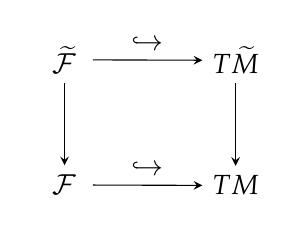
\begin{tikzpicture}
		\matrix (m) [matrix of math nodes,row sep=3em,column sep=4em,minimum width=2em]
		{
			\widetilde{\mathcal F} &    T\widetilde{M} \\
			\mathcal F	& TM    \\};
		\path[-stealth]
		(m-1-1) edge node [above] {$\hookto$} (m-1-2)
		(m-1-1) edge node [right] {} (m-2-1)
		(m-1-2) edge node [right] {} (m-2-2)
		(m-2-1) edge node [above] {$\hookto$}  (m-2-2);
		
	\end{tikzpicture}
	\newline
	then $\widetilde{\mathcal F}$ is integrable.
	
	\begin{definition}\label{fol_cov_defn}
		In the above situation we say that a foliation $\left(\widetilde{M},~ \widetilde{\mathcal F} \right)$ is the \textit{induced by} $p$ \textit{covering} of $\left(M,\mathcal F \right)$ or the $p$-\textit{lift} of $\left(M,\mathcal F \right)$. 
	\end{definition}
	\begin{remark}
		The $p$-lift of a foliation is described in  \cite{ouchi:cov_fol, xiaolu:foli_cov}.
	\end{remark}
	\begin{empt}
		If $\gamma: \left[0,1\right]\to M$ is a path which corresponds to an element of the holonomy groupoid then we denote by $\left[\gamma\right]$ its equivalence class, i.e. element of groupoid.
		There is the space of half densities $\Omega_{\widetilde{M}}^{1/2}$ on $\widetilde{M}$ which is a lift  the space of half densities $\Omega_{M}^{1/2}$ on $M$. If $L$ is a leaf of $\left(M,\mathcal F \right)$, $L'=\pi^{-1}\left( L\right)$   then a space $\widetilde{L}$ of holonomy covering of  $L$ coincides with the space of the holonomy covering of $L'$. It turns out that $L^2\left( \widetilde{\mathcal G}_{\widetilde{x}}\right)\approx L^2\left(\mathcal G_{ \pi\left(\widetilde{x}\right)} \right)$ for any $\widetilde{x} \in \widetilde{M}$.
		If $\mathcal G$ (resp. $\widetilde{\mathcal G}$) is a holonomy groupoid of $\left(M,\mathcal F \right)$ (resp. $\left(\widetilde{M},~ \widetilde{\mathcal F} \right)$) then there is the surjective map $p_{\mathcal G}:\widetilde{\mathcal G} \to \mathcal G$ given by
		\begin{equation*}
			\begin{split}
				\left[\widetilde{\gamma}\right] \mapsto \left[p \circ\widetilde{\gamma}\right].
			\end{split}
		\end{equation*}
		If the covering is finite-fold then the map $p_{\mathcal G}:\widetilde{\mathcal G} \to \mathcal G$ induces 
		a natural involutive homomorphism
		\begin{equation*}
			\begin{split}
				\Coo_c\left(\mathcal G,  \Omega_{M}^{1/2}\right) \hookto  \Coo_c\left(\widetilde{\mathcal G},  \Omega_{\widetilde{M}}^{1/2}\right).
			\end{split}
		\end{equation*}	
		Completions of $\Coo_c\left(\mathcal G,  \Omega_{M}^{1/2}\right)$ and $\Coo_c\left(\widetilde{\mathcal G},  \Omega_{\widetilde{M}}^{1/2}\right)$ with respect to given by \eqref{foli_pseudo_norm_eqn} norms gives an injective $*$- homomorphism 
		\be\label{foli_inc_eqn}
		\pi: C^*_r\left( M,\mathcal F\right) \hookto C^*_r\left(\widetilde{M},~ \widetilde{\mathcal F} \right)
		\ee
		of $C^*$-algebras. The action of the group $G\left( \left.\widetilde{M}~\right|M\right)$ of covering transformations on $\widetilde{M}$ naturally induces an action of $G\left( \left.\widetilde{M}~\right|M\right)$ on $\left(\widetilde{M},~ \widetilde{\mathcal F} \right)$.  It follows that there is the natural action   $C^*_r\left(\widetilde{M},~ \widetilde{\mathcal F} \right)$ such that 
		\be\label{foli_exp_g_eqn}
		C^*_r\left( M, \mathcal{F}\right)   = C^*_r\left(\widetilde{M},~ \widetilde{\mathcal F} \right)^{G\left( \left.\widetilde{M}~\right|M\right)}
		\ee
	\end{empt}
	
	Let $\G\left({M},~ {\mathcal F} \right)$ and $\G\left(\widetilde{M},~ \widetilde{\mathcal F} \right)$ be the holonomy groupoids of $\left({M},~ {\mathcal F} \right)$ and $\left(\widetilde{M},~ \widetilde{\mathcal F} \right)$ respectively. The natural surjective map $\G\left(\widetilde{M},~ \widetilde{\mathcal F} \right)\to\G\left({M},~ {\mathcal F} \right)$ induces the injective $*$-homomorphism $C_r^*\left(\widetilde{M},~ \widetilde{\mathcal F} \right)\hookto C^*_r\left(\widetilde{M},~ \widetilde{\mathcal F} \right)$.
	Assume both $\G\left({M},~ {\mathcal F} \right)$ and $\G\left(\widetilde{M},~ \widetilde{\mathcal F} \right)$ are Hausdorff. Let $G\left( \left.\widetilde{M}~\right|M\right)$  be the covering 	group of  $p:\widetilde M \to M$ . The $G\left( \left.\widetilde{M}~\right|M\right)$-action on $\widetilde{M}$ can be naturally extended to $\G\left(\widetilde{M},~ \widetilde{\mathcal F} \right)$ by sending $\widetilde{\ga}$ to $g\widetilde{\ga}$ for a representative path $\widetilde{\ga}$ in $ \widetilde{M}$ and $g \in G\left( \left.\widetilde{M}~\right|M\right)$. %Therefore we have a transformation groupoid $G\left( \left.\widetilde{M}~\right|M\right)\times \G\left(\widetilde{M},~ \widetilde{\mathcal F} \right)$, with the composition law $\left(g',g\widetilde{\ga} \right)\left(g, \widetilde{\ga}\right) =  \left(g'g, \widetilde{\ga}\right)$.  	 Let $G = \G\left({M},~ {\mathcal F} \right)$, $H = G\left( \left.\widetilde{M}~\right|M\right)\times \G\left(\widetilde{M},~ \widetilde{\mathcal F} \right)$, and $Z = \G\left(\widetilde{M},~ \widetilde{\mathcal F} \right)$. Clearly, the  		unit spaces are $G^0 = M$ and $H^0 = M$. Define $\rho: Z \to G^0$ and $\sigma: Z \to H^0$ by $\rho\left(\widetilde{\ga}\right)= p\left(r\left(\widetilde{\ga} \right)  \right)$  $\sigma\left( \widetilde{\ga}\right) = p\left(r\left( \widetilde{\ga}\right)  \right)$. Both are continuous open maps. The space $Z$ is
	\begin{lemma}\cite{xiaolu:foli_cov}
		Let $p:\widetilde M \to M$ be a regular covering manifold with covering group $G\left( \left.\widetilde{M}~\right|M\right)$
		$N\subset M$ a connected submanifold, and $\widetilde N$ a connected component of $p^{-1}\left( N\right) $
		Then the restriction $p_{\widetilde N}$ of $p$ to $N$ is also regular, with the covering group $G\left( \left.\widetilde{N}~\right|N\right)$ being a  	subgroup  $G\left( \left.\widetilde{M}~\right|M\right)$.
	\end{lemma}
	In particular, if $L_{\widetilde x}$ is the leave in $\left(\widetilde{M},~ \widetilde{\mathcal F} \right)$ containing $\widetilde x \in p^{-1}\left( x\right)$ , where $x \in M$,
	then $L_{\widetilde x}$ is a regular cover   of $L_x$. We denote the covering group by $G\left( \left.\widetilde{M}~\right|M\right)_x$. On the  other hand, for each $x \in M$, there is a holonomy group $\G^x_x$, and we have the holonomy group bundle $\left\{\G^x_x\right\}$  with base  $M$. If $x_1$, $x_2$ are on the same leaf, then any path $\ga$  connecting $x_1$ and $x_2$ induces an isomorphism $\ga^*: \G^{x_1}_{x_1}\xrightarrow{\cong}\G^{x_2}_{x_2}$  by mapping $\left[\ga_1\right]$ to $\left[\ga\ga_1\ga^{-1}\right]$.
	As a local homeomorphism, the covering map $p$ induces an embedding $\overline{p} : \G^{\widetilde x}_{\widetilde x}\to \G^x_x$ for each $\widetilde x \in p^{-1}\left( x\right)$.
	\begin{lemma}\cite{xiaolu:foli_cov}
		The group $\overline{p}^*_x\left(\G^{\widetilde x}_{\widetilde x}\right)$ is a normal subgroup of $G^x_x$. Equivalently,
		$\overline{p}^*_x\left( \G^{\widetilde x_1}_{\widetilde x_1}\right) =\overline{p}^*_x\left( \G^{\widetilde x_2}_{\widetilde x_2}\right)$ for $\widetilde x_1, \widetilde x_2 \in p^{-1}\left(x\right)$ if $L_{\widetilde x_1}=L_{\widetilde x_2}$,
	\end{lemma}
	Thus we may form the quotient holonomy group bundle $\left\{\G^{\widetilde x}_{\widetilde x}\right\}$ with base  $M$. There is an obvious group homomorphism $\phi_x: G\left( \left.\widetilde{M}~\right|M\right)_x \to \G^{ x}_{ x}/\G^{\widetilde x}_{\widetilde x}$ defined as follows. An element $g\in G\left( \left.\widetilde{M}~\right|M\right)_x$ corresponds to a point $x_g \in p^{-1}\left( x\right)\cap L_{\widetilde x}$ if we fix $\widetilde x$ corresponding
	to the unit $e$. A path $\ga_g$ starting at  $\widetilde x$ and ending at $g \widetilde x$ gives a loop $\pi\left(\widetilde \ga_g \right)$  in $M$ representing an element $\phi_x\left(g \right)$  in $G_x$, whose class in $\G^{ x}_{ x}/\G^{\widetilde x}_{\widetilde x}$ is uniquely defined
	by $g$. Given any $\left[\ga\right]$ in $\G^{ x}_{ x}$ there is a preimage $\widetilde \ga$ in $L_{\widetilde x}$ starting at $\widetilde x$. The point $r\left( \widetilde \ga\right) \in p^{-1}\left( x\right)\cap  L_{\widetilde x}$ corresponding to some $g\in G\left( \left.\widetilde{M}~\right|M\right)_x$. So $\phi_x$ is onto.
	\begin{definition}\cite{xiaolu:foli_cov}\label{foli_reg_cov_defn}
		The covering map $p:\left(\widetilde{M},~ \widetilde{\mathcal F} \right)\to\left({M},~ {\mathcal F} \right)$ of foliations is said to be \textit{regular} if the map $\phi$ is an isomorphism from the leaf covering group bundle to the quotient holonomy group bundle.
	\end{definition}
	
	\begin{remark}\label{foli_action_rem}
		Every regular covering map $p:\left(\widetilde{M},~ \widetilde{\mathcal F} \right)\to\left({M},~ {\mathcal F} \right)$ of foliations induces nontrivial action of $G\left( \left.\widetilde{M}~\right|M\right)$ on $C^*_r\left(\widetilde{M},~ \widetilde{\mathcal F}  \right)$ such that $$C^*_r\left(\widetilde{M},~ \widetilde{\mathcal F}  \right)^{ G\left( \left.\widetilde{M}~\right|M\right)}\cong C^*_r\left(\widetilde{M},~ \widetilde{\mathcal F}  \right).$$
	\end{remark}
	\begin{remark}\label{foli_trans_rem}
		If a map $p:\left(\widetilde{M},~ \widetilde{\mathcal F} \right)\to\left({M},~ {\mathcal F} \right)$ is regular covering of foliations  and a leaf $\widetilde L \in \widetilde M$ has no holonomy then  $g\widetilde L \neq \widetilde L$ for all nontrivial $g \in G\left( \left.\widetilde{M}~\right|M\right)$, i.e. $G\left( \left.\widetilde{M}~\right|M\right)$ principal  \ref{top_principal_defn} ly acts on leaves having no holonomy.
	\end{remark}
	
	
\chapter{Noncommutative torus and Moyal plane}\label{nt_descr_sec}
	\section{Noncommutative torus $\mathbb{T}^n_{\Theta}$}\label{nt_descr_subsec}
	\subsection{Definition of noncommutative torus $\mathbb{T}^n_{\Theta}$}
	\begin{definition}\label{nt_qirr_defn}\cite{wagner:pb}
		Denote by "$\cdot$" the scalar product on $\R^n$.
		The matrix $\Theta$ is called \emph{quite irrational} if, for all $\lambda \in \Z^n$, the condition $\exp(2\pi i \, \lambda\cdot \Theta  \mu) = 1$ for all $
		\la,\mu \in \Z^n$ implies $\lambda = 0$.
	\end{definition}
	\begin{definition}\label{nt_defn}\cite{wagner:pb}
		Let $\Theta$ be an invertible, real  skew-symmetric quite irrational $n \times n$ matrix. A \textit{noncommutative torus} $C\left(\mathbb{T}^n_{\Theta}\right)$ is the universal $C^*$-algebra generated by the set $\left\{U_k\right\}_{k \in \Z^n}$ of unitary elements which satisfy to the following relations.
		\begin{equation}\label{nt_unitary_product_eqn}
			U_k U_p = e^{-\pi ik ~\cdot~ \Theta p} U_{k + p}; ~~~   \end{equation}
	\end{definition}
	Following condition holds
	\begin{equation}\label{nt_unitary_product_comm_eqn}
		U_k U_p = e^{-2\pi ik ~\cdot~ \Theta p}U_p U_k.
	\end{equation}
	An alternative description of $\C\left(\mathbb{T}^n_{\Theta}\right)$ is such that if
	\begin{equation}\label{nt_th_eqn}
		\Th = \begin{pmatrix}
			0& \th_{12} &\ldots & \th_{1n}\\
			\th_{21}& 0 &\ldots & \th_{2n}\\
			\vdots& \vdots &\ddots & \vdots\\
			\th_{n1}& \th_{n2} &\ldots & 0
		\end{pmatrix}=\begin{pmatrix}
		0& \th_{12} &\ldots & \th_{1n}\\
		-\th_{12}& 0 &\ldots & \th_{2n}\\
		\vdots& \vdots &\ddots & \vdots\\
		-\th_{1n}& -\th_{2n} &\ldots & 0
		\end{pmatrix}
	\end{equation}
	then $C\left(\mathbb{T}^n_{\Theta}\right)$ is the universal $C^*$-algebra generated by unitary elements   $u_1,..., u_n \in U\left( C\left(\mathbb{T}^n_{\Theta}\right)\right) $ such that following condition holds
	\begin{equation}\label{nt_com_eqn}
		\begin{split}
			u_j u_k = e^{-2\pi i \theta_{jk} }u_k u_j.
		\end{split}
	\end{equation}
	Unitary  operators $u_1,..., u_n$ correspond to the standard basis of $\mathbb{Z}^n$ and they are given by
	\be\label{nt_gen_eqn}
	u_j = U_{k_j },\quad \text{ where } k_j=\left(0,...,\underbrace{ 1}_{j^{\text{th}}-\text{place}},...,0 \right)
	\ee
	\begin{defn}\label{nt_uni_defn}
		The unitary elements 
		$u_1,..., u_n \in U\left(C\left(\mathbb{T}^n_{\theta}\right)\right)$ which satisfy the relations \eqref{nt_com_eqn}, \eqref{nt_gen_eqn}
		are said to be \textit{generators} of $C\left(\mathbb{T}^n_{\Theta}\right)$. The set $\left\{U_l\right\}_{l \in \Z^n}$ is said to be the \textit{basis} of $C\left(\mathbb{T}^n_{\Theta}\right)$.
	\end{defn}

	If $a \in C\left(\mathbb{T}^n_{\Th}\right)$ is presented by a series
	\be\label{nt_series_eqn}
	a = \sum_{l \in \mathbb{Z}^{n}}c_l U_l;~~ c_l \in \mathbb{C}
	\ee
	and the series $\sum_{l \in \mathbb{Z}^{n}}\left| c_l\right| $ is convergent then from the triangle inequality it follows that the series is $C^*$-norm convergent and the following condition holds.
	\begin{equation}\label{nt_norm_estimation_eqn}
		\left\|a \right\| \le \sum_{l \in \mathbb{Z}^{n}}\left| c_l\right|.
	\end{equation}
	In particular if $\mathrm{sup}_{l \in \mathbb{Z}^n}\left(1 + \|l\|\right)^s \left|c_l\right| < \infty, ~ \forall s \in \mathbb{N}$ then $\sum_{l \in \mathbb{Z}^{n}}\left| c_l\right|< \infty $ and taking into account the equation \eqref{schwartz_z_eqn} there is the natural inclusion $\phi_\infty: \sS\left(\mathbb{Z}^n\right) \subset C\left(\mathbb{T}^n_{\Theta}\right)$ of vector spaces. If
	\be\label{nt_coo_eqn}
	\Coo\left(\mathbb{T}^n_{\Theta}\right)\bydef \phi_\infty \left( \sS\left(\mathbb{Z}^n\right)\right) \subset C\left(\mathbb{T}^n_{\Theta}\right)
	\ee
	then $\Coo\left(\mathbb{T}^n_{\Theta}\right)$ is a pre-$C^*$-algebra, and the Fourier transformation \ref{nt_fourier_eqn} yields the $\C$-isomorphism
	\be\label{nt_coo_iso_eqn}
	\Coo\left(\mathbb{T}^n\right)\cong \Coo\left(\mathbb{T}^n_{\Theta}\right).
	\ee
	\begin{empt}\label{nt_gns_empt}
		There is a  state 
		\be\label{nt_state_eqn}
		\begin{split}
			\tau: C\left(\mathbb{T}^n_{\Theta}\right) \to \C;\\
			\sum_{k \in \Z^n} a_k U_k \mapsto a_{\left(0,...,0\right) }; \quad \text{ where } a_k \in \C,
		\end{split}
		\ee
		which induces the faithful GNS representation. 
	The $C^*$-norm completion  $C\left(\mathbb{T}^n_{\Theta}\right)$ of $\Coo\left(\mathbb{T}^n_{\Theta}\right)$ is a $C^*$-algebra and there is a faithful representation
		\begin{equation}\label{nt_repr_eqn}
			C\left(\mathbb{T}^n_{\Theta}\right) \to B\left( L^2\left(C\left(\mathbb{T}^n_{\Theta}\right), \tau\right)\right) .
		\end{equation}
		(cf. Definition \ref{gns_defn}).  Similarly to the equation \eqref{from_a_to_l2_eqn} there is a $\C$-linear map 
		\begin{equation}\label{nt_to_hilbert_eqn}
			\Psi_\Th:C\left(\mathbb{T}^n_{\Theta}\right) \hookto L^2\left(C\left(\mathbb{T}^n_{\Theta}\right), \tau\right).
		\end{equation}
		If 
		\be\label{nt_xik_eqn}
		\xi_k \bydef \Psi_\Th\left(U_k \right)
		\ee 
		then from \eqref{nt_unitary_product_eqn}, \eqref{nt_state_eqn} it turns out
		\begin{equation}\label{nt_h_product_eqn}
			\tau\left(U^*_k  U_l \right) = \left(\xi_k, \xi_l \right)  = \delta_{kl},   
		\end{equation} 
		i.e. the subset $\left\{\xi_k\right\}_{k \in \mathbb{Z}^n}\subset L^2\left(C\left(\mathbb{T}^n_{\Theta}\right), \tau\right)$ is an orthogonal basis of  $L^2\left(C\left(\mathbb{T}^n_{\Theta}\right), \tau\right)$.
		Hence the Hilbert space  $L^2\left(C\left(\mathbb{T}^n_{\Theta}\right), \tau\right)$ is naturally isomorphic to the Hilbert space $\ell^2\left(\mathbb{Z}^n\right)$ given by
		\begin{equation*}
			\ell^2\left(\mathbb{Z}^n\right) = \left\{\xi = \left\{\xi_k \in \mathbb{C}\right\}_{k\in \mathbb{Z}^n} \in \mathbb{C}^{\mathbb{Z}^n}~|~ \sum_{k\in \mathbb{Z}^n} \left|\xi_k\right|^2 < \infty\right\}
		\end{equation*}
		and the $\C$-valued scalar product on $\ell^2\left(\mathbb{Z}^n\right)$ is given by
		\begin{equation}\label{nt_xi_eqn}
			\left(\xi,\eta\right)_{ \ell^2\left(\mathbb{Z}^n\right)}= \sum_{k\in \mathbb{Z}^n}    \overline{\xi}_k\eta_k.
		\end{equation}
		From \eqref{nt_unitary_product_eqn} and \eqref{nt_xik_eqn} it follows that the representation $C\left(\mathbb{T}^n_{\Theta}\right)\hookto B\left( L^2\left(C\left(\mathbb{T}^n_{\Theta}\right), \tau\right)\right)$ corresponds to the following action
		\be\label{nt_l2_eqn}
		\begin{split}
			C\left(\mathbb{T}^n_{\Theta}\right)\times  L^2\left(C\left(\mathbb{T}^n_{\Theta}\right), \tau\right)\to  L^2\left(C\left(\mathbb{T}^n_{\Theta}\right), \tau\right);\\
			U_k\xi_l = e^{-\pi ik ~\cdot~ \Theta l}\xi_{k + l} .
		\end{split}
		\ee
	\end{empt}
	

	
	\subsection{Geometry of noncommutative tori}\label{nt_geom_sec}
	\paragraph*{}
	In the below text we imply that  $\Theta$ is {quite irrational}. 
	The restriction of given by \eqref{nt_state_eqn}  state on $\Coo\left(\mathbb{T}^n_{\Theta}\right)$ satisfies to the following equation
	\begin{equation}\label{nt__smotth_state_eqn}
		\tau\left(f\right)= \widehat{f}\left(0\right)
	\end{equation}
	where $\widehat{f}$ means the Fourier transformation.
	From  $\Coo\left(\mathbb{T}^n_{\Theta} \right) \approx \SS\left( \Z^n\right)$ it follows  that there is a $\C$-linear isomorphism 
	\begin{equation}\label{nt_varphi_inf_eqn}
		\varphi_\infty: \Coo\left(\mathbb{T}^n_{\Theta} \right) \xrightarrow{\approx}  \Coo\left(\mathbb{T}^n \right).
	\end{equation} 
	such that following condition holds
	\begin{equation}\label{nt_state_integ_eqn}
		\tau\left(f \right)=  \frac{1}{\left( 2\pi\right)^n }\int_{\mathbb{T}^n} \varphi_\infty\left( f\right) ~dx.
	\end{equation}
	From \eqref{nt_state_integ_eqn} it follows that for any $a, b \in \Coo\left(\mathbb{T}^n_{\Theta}\right)$  the scalar product on $L^2\left(C\left(\mathbb{T}^n_{\Theta}\right), \tau\right)$ is given by
	\begin{equation}\label{nt_int_sc_pr_eqn}
		\left(a, b \right)= \int_{\T^n} a_{\text{comm}}^*b_{\text{comm}}dx 
	\end{equation}
	where $a_{\text{comm}}\in \Coo\left(\T^n \right)$ (resp. $b_{\text{comm}})$ is a commutative function which corresponds to $a$ (resp. $b$).
		\begin{empt}\label{nt_k_1_empt}
		If		$u_1,..., u_n \in U\left(C\left(\mathbb{T}^n_{\theta}\right)\right)$ are {generators} of $C\left(\mathbb{T}^n_{\Theta}\right)$ (cf. Definition \ref{nt_uni_defn}) then for all $\left( k_1, ..., k_n\right) \in\Z^n $ one has
		$$
		\left( k_1, ..., k_n\right)\neq 0 \quad \Rightarrow\quad	\tau \left( u_1^{k_1}\cdot ...\cdot u_n^{k_n}\right)= 0. 
		$$
		where $\tau$ is given by \eqref{nt_state_integ_eqn}. On the other hand from
		$
		\tau\left(1_{C\left(\mathbb{T}^n_{\theta}\right)}\right)= 1
		$
	 it follows that any nontrivial product $ u_1^{k_1}\cdot ...\cdot u_n^{k_n}$ is not homotopic to $1_{C\left(\mathbb{T}^n_{\theta}\right)}$ in
			 $U\left(C\left(\mathbb{T}^n_{\theta}\right)\right)$. Similarly to \cite{varilly:noncom} one can deduce the following
			\be\label{nt_k_1_eqn}
		K_1\left(C\left(\mathbb{T}^n_{\theta}\right)\right)= \Z\left[u_1\right]\oplus ... \oplus \Z\left[u_n\right]
			\ee
			where $K_1$ means the $K_1$-functor (cf. \cite{blackadar:ko}).
	\end{empt}
	\begin{defn}\label{nt_symplectic_defn}
		If  $\Theta$ is non-degenerate, that is to say,
		$\sigma(s,t) \stackrel{\mathrm{def}}{=} s\.\Theta t$ to be \textit{symplectic}. This implies even
		dimension, $n = 2N$. One then selects
		\begin{equation}\label{nt_simpectic_theta_eqn}
			\Theta = \theta J
			\stackrel{\mathrm{def}}{=} \th \begin{pmatrix} 0 & 1_N \\ -1_N & 0 \end{pmatrix}
		\end{equation}
		where  $\th > 0$ is defined by $\th^{2N} \stackrel{\mathrm{def}}{=} \det\Theta$.
		Denote by
		\be\label{nt_symplectic_eqn}
		\begin{split}
	\Coo\left(\mathbb{T}^{2N}_\th\right)\stackrel{\mathrm{def}}{=}\Coo\left(\mathbb{T}^{2N}_\Th\right),\\
	C\left(\mathbb{T}^{2N}_\th\right)\stackrel{\mathrm{def}}{=}C\left(\mathbb{T}^{2N}_\Th\right).
		\end{split}
\ee
	\end{defn}
	\paragraph*{}
	The space $\Coo\left(\T^n_{\Theta}\right)$ is a dense subspace of  the Hilbert space $L^2\left(C\left(\mathbb{T}^n_{\Theta}\right), \tau\right)$. Let  $\L^\dagger\left(\Coo\left(\mathbb{T}^n_{\Theta}\right)\right)$ be a given by  the equation \eqref{l_dag_eqn} $O^*$-algebra. Denote by $\delta_{\mu}\in \L^\dagger\left(\Coo\left(\mathbb{T}^n_{\Theta}\right)\right)$ ($\mu = 1,\dots, n$) the analogues of the partial derivatives  on $C^{\infty}(\mathbb{T}^n)$ which are derivations on the algebra $C^{\infty}(\mathbb{T}^n_{\Theta})$ given by
	\be\label{nt_diff_eqn}
k = \left(k_1,..., k_n\right)\quad \Rightarrow\quad	\delta_{\mu}(U_k)=ik_{\mu} U_k.
	\ee
	These derivations have the following property
	$$
	\delta_{\mu}(a^*)=-(\delta_{\mu}a)^*,
	$$
	and also satisfy  the integration by parts formula
	$$\tau(a\delta_{\mu}b)=-\tau((\delta_{\mu}a)b),\quad a,b\in C^{\infty}(\mathbb{T}^n_{\Theta}).$$
From 	the equation \eqref{nt_unitary_product_eqn}	one has
	\bean
		\delta_\mu\left(U_k U_l \right)=  e^{-\pi ik ~\cdot~ \Theta l}	\delta_\mu\left(U_{k+l} \right)= i\left(k_\mu + l_\mu \right) e^{-\pi ik ~\cdot~ \Theta l}U_{k+l} =\\=
		i\left(k_\mu + l_\mu \right)U_k U_l= \left( ik_\mu U_k\right) U_l + U_k \left( il_\mu U_l\right)= \left( \delta_\mu U_k\right) U_l + U_k \left( \delta_\mu U_l\right),
	\eean
	and from the above equation one has a Leibniz rule
	\be\label{nt_le_eqn}
\forall a, b \in C^{\infty}(\mathbb{T}^n_{\Theta})\quad \delta_{\mu}\left( a\cdot b\right)  =\left( \delta_\mu a\right)\cdot b + a\cdot \left( \delta_\mu b\right)
	\ee
	where $\cdot$ means the product of the involutive algebra $\Coo\left(\mathbb{T}^n_{\Theta}\right)$.
	The spectral triple describing the noncommutative geometry of noncommutative $n$-torus consists of the algebra $C^{\infty}(\mathbb{T}^n_{\Theta})$, the Hilbert space $\mathcal{H}=L^2\left(C\left(\mathbb{T}^n_{\Theta}\right), \tau\right)\otimes\mathbb{C}^{m}$, where $m=2^{[n/2]}$ with  the representation  $\pi\otimes 1_{\mathbb{M}_n\left(\C\right) }:C^{\infty}(\mathbb{T}^n_{\Theta})\to B\left( \H\right) $  where $\pi: C^{\infty}(\mathbb{T}^n_{\Theta})\to B\left( L^2\left(C\left(\mathbb{T}^n_{\Theta}\right), \tau\right)\right)$ is given by \eqref{nt_repr_eqn}.
	The Dirac operator is given by
	\begin{equation}\label{nt_dirac_eqn}
		D\stackrel{\mathrm{def}}{=}\sum_{\mu =1}^{n}\delta_{\mu} \otimes\gamma^{\mu}\in \L^\dagger\left(\Coo\left(\mathbb{T}^n_{\Theta}\right)\otimes\C^m\right),
	\end{equation}
	where $\delta_{\mu}$ is given by \eqref{nt_diff_eqn}, seen as an unbounded self-adjoint operator on $L^2\left(C\left(\mathbb{T}^n_{\Theta}\right), \tau\right) $ and $\gamma^{\mu}$s are Clifford (Gamma) matrices in $\mathbb{M}_m(\mathbb{C})$ satisfying the relation
	\be\label{nt_gam_eqn}\gamma^\mu\gamma^\nu+\gamma^\nu\gamma^\mu=2\delta_{\mu\nu} 1_{\mathbb{M}_m(\mathbb{C})}.\ee
	There is a spectral triple 
	\begin{equation}\label{nt_sp_tr_eqn}
		\left( C^{\infty}(\mathbb{T}^n_{\Theta}),L^2\left(C\left(\mathbb{T}^n_{\Theta}\right), \tau\right)\otimes\mathbb{C}^{m},D\right).
	\end{equation}
There is an alternative description of $D$. Any $b \in \Coo\left(\T^n\right)$ can be regarded as $f_b \in  \Coo\left(\R^n\right)$ which is $\Z^n$-periodic, i.e. it is invariant with respect to $\Z^n$-shifts. If $x_1,..., x_n$ are coordinates of $\R^n$ then for all $\mu= 1,..., n$ 
the partial derivation $\frac{\partial f_b}{\partial x_\mu}$ is smooth and  $\Z^n$-periodic. We write $\frac{\partial b}{\partial x_\mu}$ instead of $\frac{\partial f_b}{\partial x_\mu}$ so for all $\mu= 1,..., n$ one can assume $\frac{\partial b}{\partial x_\mu}\in \Coo\left(\T^n\right)$, i.e. there is an operator $\frac{\partial}{\partial x_\mu}\in \L^\dagger\left(  \Coo\left(\T^n\right)\right) $. Using the given by \eqref{nt_varphi_inf_eqn} $\C$-linear isomorphism  $\varphi_\infty:\Coo\left(\mathbb{T}^n_{\Theta} \right) \cong \Coo\left(\mathbb{T}^n \right)$   one can set 
	\be\label{nt_ddx_eqn}
	\frac{\partial}{\partial x_\mu}\in \L^\dagger\left( \Coo\left(\mathbb{T}^n_{\Theta} \right) \right)
	\ee
Elements of the basis $U_k$ and generators $u_\mu$ (cf. Definition  \ref{nt_uni_defn})  $U_k$ correspond to  $\Z^n$-periodic maps  $\R^n \to \C$ such that 
\bean
\\
U_k: x \mapsto e^{2\pi i k \cdot x},\\
u_\mu : x \mapsto e^{2\pi i x_\mu}\quad x = \left(x_1, ..., x_n\right)
\eean
Using chain rule one has
\be\label{nt_chain_eqn}
\frac{\partial}{\partial x_\mu} = \frac{1}{2\pi i}u^*\frac{\partial}{\partial u_\mu}, 
\ee	
so $\frac{\partial}{\partial u_\mu}$ can be regarded as a $\C$=linear map 
\be\label{nt_chainu_eqn}
\frac{\partial}{\partial u_\mu}: \Coo\left(\R^n \right)\to \Coo\left(\R^n \right). 
\ee
Otherwise one has
\be\label{nt_chaind_eqn}
\delta_\mu =  i u_\mu \frac{\partial}{\partial u_\mu} = 2\pi \frac{\partial}{\partial x_\mu} ,
\ee	
so the equation \eqref{nt_dirac_eqn}  can be rewritten by the following way
	\begin{equation}\label{nt_dirac_u_eqn}
	D\stackrel{\mathrm{def}}{=}\sum_{\mu =1}^{n}\delta_{\mu} \otimes\gamma^{\mu}= i \sum_{\mu =1}^{n} u_\mu \frac{\partial}{\partial u_\mu} \otimes\gamma^{\mu}\in \L^\dagger\left(\Coo\left(\mathbb{T}^n_{\Theta}\right)\otimes\C^m\right).
\end{equation}
Form the equation  \eqref{nt_diff_eqn} it follows that 
Let $b \in \Coo\left(\mathbb{T}^n_{\Theta} \right)$, $~\xi\in \C^m$
\be\label{nt_ga_eqn}
\begin{split}
\left( \left(u^*_\mu \otimes 1_{\mathbb{M}_m\left(\C\right)} \right)  \left[ D, u_\mu \otimes 1_{\mathbb{M}_m\left(\C\right)} \right]\right)\left( b\otimes \xi\right) =\\
\left(u^*_\mu \otimes 1_{\mathbb{M}_m\left(\C\right)} \right)\left(  D\left( u_\mu b\otimes \xi\right) - \left(u_\mu \otimes 1_{\mathbb{M}_m\left(\C\right)} \right) D\left( b\otimes \xi\right) \right).
\end{split}
 \ee
From the definition \eqref{nt_dirac_u_eqn} of the Dirac operator and tha chain rule \eqref{nt_le_eqn} it follows that 
\bean
D\left( u_\mu b\otimes \xi\right)= \left( \sum_{\mu =1}^{n}\delta_{\mu} \otimes\gamma^{\mu}\right)\left( u_\mu b\otimes \xi\right)= i \left( u_\mu \cdot b\right) \otimes\xi +  \sum_{\mu =1}^{n}u_\mu \delta_\mu b \otimes \ga^\mu\xi,\\
\left(u_\mu \otimes 1_{\mathbb{M}_m\left(\C\right)} \right) D\left( b\otimes \xi\right)= \sum_{\mu =1}^{n}u_\mu \delta_\mu b \otimes \ga^\mu\xi
\eean
The substitution of the above equation into \eqref{nt_ga_eqn} yields the following
\bean
\left( \left(u^*_\mu \otimes 1_{\mathbb{M}_m\left(\C\right)} \right)  \left[ D, u_\mu \otimes 1_{\mathbb{M}_m\left(\C\right)} \right]\right)\left( b\otimes \xi\right) =\\
\left(iu^*_\mu  \otimes 1_{\mathbb{M}_m\left(\C\right)}\right) \left( u_\mu b\otimes \ga \xi\right) = i\left(b \otimes \ga^\mu \xi \right).
\eean
or, equivalently
\be\label{nt_ga'_eqn}
\left(u^*_\mu \otimes 1_{\mathbb{M}_m\left(\C\right)} \right)  \left[ D, u_\mu \otimes 1_{\mathbb{M}_m\left(\C\right)} \right]= i 1_{\Coo\left(\mathbb{T}^n_{\Theta} \right)}\otimes \ga^\mu.
\ee
If $\Om^1_D$ is a {module of differential forms associated} with the given by \eqref{nt_sp_tr_eqn}  spectral triple (cf. Definition \ref{ass_cycle_defn}) then $\left(u^*_\mu \otimes 1_{\mathbb{M}_m\left(\C\right)} \right)  \left[ D, u_\mu \otimes 1_{\mathbb{M}_m\left(\C\right)} \right]\in \Om^1_D$ and taking into account \eqref{nt_ga'_eqn} one has
\be\label{nt_ga_in_eqn}
1_{\Coo\left(\mathbb{T}^n_{\Theta} \right)}\otimes \ga^\mu\in \Om^1_D.
\ee
\section{Moyal plane}
	
	\begin{defn}\cite{moyal_spectral}
		Denote the \textit{Moyal plane} product $\star_\th$ on $\SS\left(\R^{2N} \right)$ given by
		\begin{equation}\label{mp_prod_eqn}
			\left(f \star_\th h \right)\left(u \right)= \int_{y \in \R^{2N} } f\left(u - \frac{1}{2}\Th y\right) g\left(u + v \right)e^{2\pi i y \cdot v }  dydv
		\end{equation}
		
		where $\Th$ is given by \eqref{nt_simpectic_theta_eqn}.
	\end{defn}
	There is the tracial property \cite{moyal_spectral} of the Moyal product
	\begin{equation}\label{nt_tracial_prop}
		\int_{\R^{2N}} \left( f\star_\th g\right) \left(x \right)dx =  \int_{\R^{2N}}  f\left(x \right) g\left(x \right)dx.
	\end{equation}
	The Fourier transformation of the star product satisfies to the following condition.
	\begin{equation}\label{mp_fourier_eqn}
		\mathcal{F}\left(f \star_\th g\right) \left(x \right) =    	\int_{\R^{2N}}\mathcal{F}{f}\left(x-y \right) \mathcal{F}{g}\left(y\right)e^{ \pi i  y \cdot \Th x }~dy.
	\end{equation}
	\begin{prop}\label{mp_factor_prop}\cite{moyal_spectral}
		The algebra $\SS\left(\R^{2N}, \star_\th \right)$  has the (nonunique) factorization property:
		for all $h \in  \SS\left(\R^{2N} \right)$ there exist $f,g \in  \SS\left(\R^{2N} \right)$ that $h = f \star_\th g$.
	\end{prop}
	% Denition 2.8   
	\begin{defn}\label{mp_mult_defn}\cite{varilly_bondia:phobos}  !!! REPLACE TO S 2!!!!
		\label{df:Moyal-alg}	Denote by $\SS'\left( \R^{n}\right) $ the vector space dual to $\SS\left( \R^{n}\right) $, i.e. the space of continuous functionals on $\SS\left( \R^{n}\right)$.
		The Moyal product can be defined, by duality, on larger sets than
		$\SS\left(\R^{2N}\right)$. For $T \in \SS'\left(\R^{2N}\right)$, write the evaluation on $g \in \SS\left(\R^{2N}\right)$ as
		$\<T, g> \in \C$; then, for $f \in \SS$ we may define $T \star_{\theta} f$ and
		$f \star_{\theta} T$ as elements of~$\SS'\left(\R^{2N}\right)$ by
		\begin{equation}\label{mp_star_ext_eqn}
			\begin{split}
				\<T \star_{\theta} f, g> \stackrel{\mathrm{def}}{=} \<T, f \star_{\theta} g>\\
				\<f \star_{\theta} T, g> \stackrel{\mathrm{def}}{=} \<T, g \star_{\theta} f>	\end{split}
		\end{equation}  using the continuity of the
		star product on~$\SS\left(\R^{2N}\right)$. Also, the involution is extended to  by
		$\<T^*,g> \stackrel{\mathrm{def}}{=} \overline{\<T,g^*>}$.	
		%	We shall soon argue~\cite{varilly_bondia:phobos} that if $T \in \SS'\left(\R^{2N}\right)$ and	$f \in \SS\left(\R^{2N}\right)$, then $T \star_{\theta} f,\,f \star_{\theta} T \in C^\infty(\R^{2N})$.
		Consider the left  and right multiplier algebras:
		\begin{equation}\label{mp_multi_eqn}
			\begin{split}
				\M_L^\th
				&\stackrel{\mathrm{def}}{=} \set{T \in \SS'(\R^{2N}) : T \star_{\theta} h \in \SS(\R^{2N})
					\text{ for all } h \in \SS(\R^{2N})},
				\\
				\M_R^\th
				&\stackrel{\mathrm{def}}{=} \set{T \in \SS'(\R^{2N}) : h \star_{\theta} T \in \SS(\R^{2N})
					\text{ for all } h \in \SS(\R^{2N})},\\
				\M^\th &\stackrel{\mathrm{def}}{=} \M_L^\th \cap \M_R^\th.\\
			\end{split}
		\end{equation} 
	\end{defn}
	In \cite{varilly_bondia:phobos} it is proven that
	\bea\label{mp_mult_distr}
	\M_R^\th \star_{\theta} \SS'\left(\R^{2N}\right) = \SS'\left(\R^{2N}\right) \text{ and }
	\SS'\left(\R^{2N}\right) \star_{\theta} \M_L^\th = \SS'\left(\R^{2N}\right),\\
	\label{mp_parial_mult_eqn}
	\partial_j S \times f = 	\partial_j \left( S \times f \right) - f \times \partial_j S \quad \forall S \in \M_L^\th \quad \forall f \in \SS(\R^{2})
	\eea
	
	
	It is known \cite{moyal_spectral} that the domain of  the Moyal plane product can be extended up to $L^2\left(\R^{2N} \right)$. 
	
	\begin{lem}\label{nt_l_2_est_lem}\cite{moyal_spectral}
		If $f,g \in L^2 \left(\R^{2N} \right)$, then $f\star_\th g \in L^2 \left(\R^{2N} \right)$ and $\left\|f\right\|_{\mathrm{op}} < \left(2\pi\th \right)^{-\frac{N}{2}} \left\|f\right\|_2$.
		where	$\left\|\cdot\right\|_{2}$ be the $L^2$-norm given by
		\begin{equation}\label{nt_l2_norm_eqn}
			\left\|f\right\|_{2} \stackrel{\mathrm{def}}{=} \left|\int_{\R^{2N}} \left|f\right|^2 dx \right|^{\frac{1}{2}}.
		\end{equation}
		and the operator norm
		\be\label{mp_op_eqn}
		\|T\|_{\mathrm{op}} \stackrel{\mathrm{def}}{=}\sup\set{\|T \star g\|_2/\|g\|_2 : 0 \neq g \in L^2\left( \R^{2N})\right) }
		\ee 
	\end{lem}
	%\begin{rem}\label{norm_remark}
	%	Since $\SS\left(\R{2N} \right)$ is dense in $L^2\left(\R{2N} \right)$ the operator norm is given by $\|T\|_{\mathrm{op}} =\sup\set{\|T \star g\|_2/\|g\|_2 : 0 \neq g \in \SS\left( \R^{2N}\right) }$ 
	%\end{rem}
	
	\begin{defn}\label{mp_star_alg_defn}
		Denote by $\SS\left(\R^{2N}_\th \right)$  (resp. $L^2\left(\R^{2N}_\th \right)$ ) the operator algebra  which is $\C$-linearly isomorphic to $\SS\left(\R^{2N} \right)$  (resp. $L^2\left(\R^{2N} \right)$ ) and product coincides with  $\star_\th$. Both  $\SS\left(\R^{2N}_\th \right)$ and $L^2\left(\R^{2N}_\th \right)$ act on the Hilbert space $L^2\left(\R^{2N} \right)$. Denote by
		\begin{equation}\label{mp_psi_th_eqn}
			\Psi_\th:  \SS\left(\R^{2N} \right)\xrightarrow{\approx}\SS\left(\R^{2N}_\th \right)
		\end{equation}
		the natural $\C$-linear isomorphism.  
	\end{defn}
	
	\ref{mp_nt_op_empt}   !!! CHANGE !!!
	\begin{defn}\label{nt_r_2_N_repr_defn}\cite{moyal_spectral} Let $\SS'\left(\R^{2N} \right)$ be a vector space dual to $\SS\left(\R^{2N} \right)$. Denote by $C_b\left(\R^{2N}_\th\right)\stackrel{\mathrm{def}}{=} \set{T \in \SS'\left(\R^{2N}\right) : T \star_\th g \in L^2\left(\R^{2N}\right) \text{ for all } g \in L^2(\R^{2N})}$, provided with the given by \eqref{mp_op_eqn} operator norm $	\|\cdot\|_{\mathrm{op}}$.
		Denote by $C_0\left(\R^{2N}_\th \right)$ the operator norm completion of $\SS\left(\R^{2N}_\th \right).$  
	\end{defn}
	\begin{rem}
		Obviously $\SS\left(\R^{2N}_\th\right)  \hookto C_b\left(\R^{2N}_\th\right)$. But $\SS\left(\R^{2N}_\th\right)$ is not dense in $C_b\left(\R^{2N}_\th\right)$, i.e. $C_0\left(\R^{2N}_\th\right) \subsetneq C_b\left(\R^{2N}_\th\right)$  (cf. \cite{moyal_spectral}).
	\end{rem}
	
	\begin{rem}
		$L^2\left(\R^{2N}_\th\right)$ is the $\|\cdot\|_2$ norm completion of $\SS\left(\R^{2N}_\th\right)$ hence 
		from the Lemma \ref{nt_l_2_est_lem} it follows that 
		\begin{equation}\label{mp_2_op_eqn}
			L^2\left(\R^{2N}_\th\right) \subset C_0\left(\R^{2N}_\th\right).
		\end{equation} 
	\end{rem}
	\begin{rem}
		Notation of the Definition \ref{nt_r_2_N_repr_defn} differs from \cite{moyal_spectral}. Here symbols $A_\th, \A_\th, A^0_\th$ are replaced with $C_b\left(\R^{2N}_\th\right), \SS\left(\R^{2N}_\th\right), C_0\left(\R^{2N}_\th\right)$ respectively.
	\end{rem}
	\begin{rem}
		The $\C$-linear space $C_0\left(\R^{2N}_\th \right)$ is not isomorphic to $C_0\left(\R^{2N}\right)$. 
	\end{rem}
	
	
	There are elements $\left\{f_{nm}\in\SS\left(\R^{2} \right)\right\}_{m,n \in \N^0}$, described in \cite{varilly_bondia:phobos}, which satisfy to the following Lemma. 
	\begin{lem}\label{mp_osc_lem} {\rm\cite{varilly_bondia:phobos}}
		\label{lm:osc-basis}
		Let $m,n,k,l \in \N$. Then $f_{mn} \star_\th f_{kl} = \delta_{nk}f_{ml}$
		and $f_{mn}^* = f_{nm}$. Thus $f_{nn}$ is an orthogonal projection and
		$f_{mn}$ is nilpotent for $m \neq n$. Moreover ,
		$\left\langle f_{mn}, f_{kl}\right\rangle  = %2^N\,
		\delta_{mk}\,\delta_{nl}$. The family
		$\set{f_{mn} : m,n\in \N^0} \subset \sS\left( \mathbb{R}^{2}\right) \subset L^2(\R^{2})$ is an
		orthogonal basis.
	\end{lem}
	\begin{remark}
		One has 
		\be\label{nt_dmn_eqn}
		\int_{\R^2} f_{mn} = \delta_{mn}.
		\ee
	\end{remark}
	
	
	%Theorem 6: 
	\begin{prop}\label{mp_fmn_prop}\cite{moyal_spectral,varilly_bondia:phobos}
		Let $N = 1$. Then $\SS\left(\R^{2N}_\th\right)=\SS\left(\R^{2}_\th\right) $ has a Fr\'echet algebra isomorphism with
		the matrix algebra of rapidly decreasing double sequences
		$c = (c_{mn})$ of complex numbers such that, for each $k \in \N$,
		\begin{equation}\label{mp_matr_norm}
			r_k(c) \stackrel{\mathrm{def}}{=} \biggl( \sum_{m,n=0}^\infty
			\th^{2k}  \left( m+\half\right)^k \left( n+\half\right)^k |c_{mn}|^2 \biggr)^{1/2}
		\end{equation}
		
		is finite, topologized by all the seminorms $(r_k)$; via the
		decomposition $f = \sum_{m,n=0}^\infty c_{mn} f_{mn}$ of~$\SS(\R^2)$ in
		the $\{f_{mn}\}$ basis.
		The twisted product $f \star_\th g$ is
		the matrix product $ab$, where
		\begin{equation}\label{mp_mult_eqn}
			\left( ab\right)_{mn} \stackrel{\mathrm{def}}{=} \sum_{k= 0}^{\infty} a_{\mu\nu}b_{kn}.
		\end{equation}
		
		For $N > 1$, $\Coo\left(\R^{2N}_\th\right)$ is isomorphic to the (projective) tensor product
		of $N$ matrix algebras of this kind, i.e.
		\begin{equation}\label{mp_tensor_prod}
			\SS\left(\R^{2N}_\th\right) \cong \underbrace{\SS\left(\R^{2}_\th\right)\otimes\dots\otimes\SS\left(\R^{2}_\th\right)}_{N-\mathrm{times}}
		\end{equation}
		with the projective topology induced by seminorms $r_k$ given by \eqref{mp_matr_norm}.	
	\end{prop}
	\begin{rem}
		If $A$ is  $C^*$-norm completion of the matrix algebra with the norm \eqref{mp_matr_norm} then $A \approx \mathcal K$, i.e.
		\begin{equation}\label{mp_2_eqn}
			C_0\left(\R^{2}_\th\right) \approx \mathcal K.
		\end{equation}
		Form \eqref{mp_tensor_prod} and \eqref{mp_2_eqn} it follows that
		\begin{equation}\label{mp_2N_eqn}
			C_0\left(\R^{2N}_\th\right) \cong \underbrace{C_0\left(\R^{2}_\th\right)\otimes\dots\otimes C_0\left(\R^{2}_\th\right)}_{N-\mathrm{times}} \approx \underbrace{\mathcal K\otimes\dots\otimes\mathcal K}_{N-\mathrm{times}} \approx \mathcal K
		\end{equation}
		where $\otimes$ means minimal or maximal tensor product ($\mathcal{K}$ is nuclear hence both products coincide).
		
	\end{rem}
	
	\begin{definition}\cite{varilly_bondia:phobos}
		%Denition 6.
		For $s, t \in\R$ we denote by $\G_{s,t}$ the Hilbert space obtained by completing $\sS\left( \R^2 \right)$  with
		respect to the norm
		$$
		\left\|\sum_{m,n = 0}^\infty c_{mn} f_{mn}\right\|= \sqrt{\sum_{m,n = 0}^\infty \left(2m + 1\right)^s \left(2n + 1\right)^t \left| c_{mn}\right|^2 }
		$$
		
	\end{definition}
	
	Denote by 
	\be
	\mathcal{I}_{s,t}\bydef \G_{s,0}\times \G_{0,t} = \left\{f\times g~ \left|~ f\in \G_{s,0}, \quad g\in \G_{0,t}  \right|\right\}
	\ee
	
	
	
	\begin{empt}\label{nt_m_planes_empt}\cite{moyal_spectral}
		By plane waves we understand all functions of the form
		$$
		x \mapsto \exp(ik\cdot x) 
		$$
		for $k\in \R^{2N}$.  One obtains for the Moyal
		product of plane waves:
		\begin{equation}\label{mp_wave_prod_eqn}
			\begin{split}
				\exp\left(ik\cdot\right) \star_{\Theta}\exp\left(ik\cdot\right)=\exp\left(ik\cdot\right) \star_{\theta}\exp\left(ik\cdot\right)= \exp\left(i\left( k+l\right) \cdot\right) e^{-\pi i k \cdot \Th l}.
			\end{split}
		\end{equation}
		It is proven in \cite{moyal_spectral} that plane waves lie in $C_b\left(\R^{2N}_\th \right)$. 	
	\end{empt}
	
	
	\begin{empt}\label{mp_scaling_empt}
		
		
		
		Let us consider the unitary dilation operators $E_a$ given
		by
		$$
		E_af(x) \stackrel{\mathrm{def}}{=} a^{N/2} f(a^{1/2}x),
		$$
		It is proven in \cite{moyal_spectral} that
		\begin{equation}\label{eq:starscale}
			f {\star_{\theta}} g =
			(\th/2)^{-N/2} E_{2/\th}(E_{\th/2}f \star_2 E_{\th/2}g).
		\end{equation}
		We can simplify our construction by setting $\th = 2$. Thanks to
		the scaling relation~\eqref{eq:starscale} any qualitative result can is true if it is true in case of 
		$\th = 2$. We use the following notation
		\begin{equation}\label{mp_times_eqn}
			f {\times} g\stackrel{\mathrm{def}}{=}f {\star_{2}} g
		\end{equation}
		
		
		Introduce the symplectic Fourier transform $F$ by
		\begin{equation}
			Ff(x) \stackrel{\text{def}}{=} (2\pi)^{-N} \int f(t) e^{ix \cdot Jt} \,d^{2N}t; \quad 	\widetilde Ff(x) \stackrel{\text{def}}{=} (2\pi)^{-N} \int f(t) e^{ix \cdot Jt} \,d^{2N}t; 
			\label{eq:Fsympl}
		\end{equation}
		The \textit{twisted convolution} \cite{varilly_bondia:phobos} $f\diamond g$ is defined by
		\begin{equation}\label{nt_diamond_eqn}
			f\diamond g \left(u \right) \stackrel{\text{def}}{=} \int f\left(u - t\right)  g\left(t \right)e^{-iu \cdot J t}  dt.
		\end{equation}
		Following conditions hold \cite{varilly_bondia:phobos}:
		\bea\label{nt_prod_duality_eqn}
		\mathcal{F}\left(f \times g \right) = \mathcal{F} f \diamond  \sF g ;\quad \mathcal{F}\left(f \diamond g \right) = \mathcal{F} f \times \mathcal{F} g;\\
		\label{nt_prodf_duality}
		f \times g = Ff \diamond g = f \diamond  \widetilde Fg;  \quad f \diamond g = Ff \times g = f \times \widetilde F g;\\
		\label{nt_prod_ass_eqn}
		\left( f \times g \right) \times h= f \times \left(g \times h\right);  \quad \left( f \diamond g \right) \diamond h= f \diamond \left(g \diamond h\right);\\
		\label{nt_prod_*_eqn}
		\left( f \times g \right)^* = g^*\times h^*;  \quad \left( f \diamond g \right)^* = g^*\diamond h^*.
		\eea
		
	\end{empt} 
	\	
	
	\begin{defn}
		\label{df:Gst}\cite{moyal_spectral}
		We may as well introduce more Hilbert spaces $\G_{st}$ (for
		$s,t \in \R$) of those 
		$$
		f \in \SS'(\R^2) = \sum_{m,n = 0}^\infty c_{mn} f_{mn}
		$$ for which the following sum
		is finite:
		$$
		\|f\|_{st}^2 \stackrel{\mathrm{def}}{=} \sum_{m,n=0}^\infty
		(m+\half)^s (n+\half)^t |c_{mn}|^2.
		$$
		%	We define $\G_{st}$, for $s,t$ now in $\R^N$, as the tensor product	of Hilbert spaces $\G_{s_1t_1} \oxyox \G_{s_Nt_N}$. In other	words, the elements $(2\pi)^{-N/2} 	(m+\half)^{-s/2} (n+\half)^{-t/2} f_{mn}$ (with an obvious multiindex 	notation), for $m,n \in \N^N$, are declared to be an orthonormal basis
		for~$\G_{st}$.
	\end{defn}
	%\begin{rem}\cite{varilly_bondia:phobos}
	%	Observe that 
	%	\begin{equation*}
	%\G_{0,0} = L^2\left( \R^2\right)
	%	\end{equation*}
	
	%	$\G_{0,0} = L^2\left( \R^2\right)$. 
	%\end{rem}
	\begin{rem}\label{mp_l2_rem}
		It is proven in \cite{varilly_bondia:phobos} $f, g \in L^2\left( \R^2\right)$, then $f\times g \in L^2\left( \R^2\right)$ and $\left\|f\times g  \right\|\le\left\|f \right\|\left\| g  \right\|$.
		Moreover , $f \times g$ lies in $C_0\left( \R^2\right)$ : the continuity follows by adapting the analogous argument for (ordinary) convolution. 
	\end{rem}
	%	\begin{rem}\label{mp_smooth_rem}\cite{varilly_bondia:deimos}
	%	The Leibniz formula assures us that $f \times g \in C_0^m\left(\R^2 \right)$ 
	%	 whenever
	%	 $$
	% 	f, g \in \bigcup \left\{\G_{st}~|~ s > 2m, t > 2m, s + t > 4m + 2\right\}
	% 	$$
	% 	analogously to what happens in the usual \operatorname{loc}olev spaces, the distributions in $\G_{st}$ grow more
	% 	regular as $s, t$ become larger in a suitable way.
	%	\end{rem}
	\begin{rem}\label{mp_ss_rem}
		It is shown in \cite{varilly_bondia:phobos} that 
		\begin{equation}\label{mp_ssin_eqn}
			\SS\left( \R^2\right) = \bigcap_{s, t \in \R} \G_{st}.
		\end{equation}
	\end{rem}
	
	\begin{empt}\label{mp_coord_constr}
		This part contains a useful equations proven in \cite{varilly_bondia:phobos}.
		There are coordinate functions $p,q$ on $\R^2$ such that for any $f \in \SS\left( \R^2\right)$ following conditions hold
		\begin{equation}\label{mp_pq_mult_eqn}
			\begin{split}
				q \times f = \left(q + i \frac{\partial}{\partial p} \right)  f; ~~p \times f = \left(p - i \frac{\partial}{\partial q} \right)  f;\\
				f \times q = \left(q - i \frac{\partial}{\partial p} \right)  f; ~~f \times p = \left(p + i \frac{\partial}{\partial q} \right)  f.
			\end{split}
		\end{equation}
		From $q \times f, f \times q,p  \times f, f \times p \in \SS\left(\R^{2N} \right)$ it follows that $p, q \in \M^2$ (cf. \eqref{mp_multi_eqn}). From 
		\eqref{mp_mult_distr} it follows that
		\begin{equation}\label{mp_pq_mult}
			\begin{split}
				q \times \SS'\left(\R^{2N} \right) \subset \SS'\left(\R^{2N} \right); ~~p \times \SS'\left(\R^{2N} \right) \subset \SS'\left(\R^{2N} \right);\\
				\SS'\left(\R^{2N} \right) \times q \subset \SS'\left(\R^{2N} \right); ~~\SS'\left(\R^{2N} \right) \times p \subset \SS'\left(\R^{2N} \right).
			\end{split}
		\end{equation}
		If $f \in \SS'\left( \R^2\right)$ then from \eqref{mp_pq_mult_eqn} it follows that
		\begin{equation}\label{mp_partial_eqn}
			\frac{\partial}{\partial p} f = -iq \times f + i f \times q, ~~  \frac{\partial}{\partial q} f = ip \times f - i f \times p
		\end{equation}
		
		
		If 
		\begin{equation}\label{mp_ham_eqn}
			\begin{split}
				a \stackrel{\mathrm{def}}{=} \frac{q + ip}{\sqrt{2}}, ~~\overline{a} \stackrel{\mathrm{def}}{=} \frac{q - ip}{\sqrt{2}},\\
				\frac{\partial}{\partial a}\stackrel{\mathrm{def}}{=} \frac{\partial_q + i\partial_p}{\sqrt{2}}, ~~ \frac{\partial}{\partial \overline{a}}\stackrel{\mathrm{def}}{=} \frac{\partial_q - i\partial_p}{\sqrt{2}},\\
				H \stackrel{\mathrm{def}}{=}a \overline{a}= \frac{1}{2}\left(p^2 + q^2 \right) , \\
				\overline{a}\times a = H - 1, ~~ a \times \overline{a} = H + 1
			\end{split}
		\end{equation}
		then
		\begin{equation}\label{mp_ap_eqn}
			\begin{split}
				a \times f = af + \frac{\partial f}{\partial \overline{a}}, ~~ f \times a = af - \frac{\partial f}{\partial \overline{a}}, \\
				\overline{a} \times f = \overline{a}f - \frac{\partial f}{\partial a}, ~~ f \times a = \overline{a}f + \frac{\partial f}{\partial a}, \\
			\end{split}
		\end{equation} \begin{equation}\label{mp_ham_act_eqn}
			\begin{split}
				H\times f_{mn} = (2m + 1) f_{mn};~~f_{mn} \times H = 2(n + 1)f_{mn}
			\end{split}
		\end{equation} 
		\begin{equation}\label{mp_hamd_act_eqn}
			\begin{split}
				a \times f_{mn} = \sqrt{2m}f_{m-1,n};~~ f_{mn}\times a = \sqrt{2n + 2} f_{m, n+1};\\
				\overline{a} \times f_{mn} = \sqrt{2m+2}f_{m+1,n};~~ f_{m+1,n}\times \overline{a} = \sqrt{2n} f_{m, n-1}.
			\end{split}
		\end{equation} 
		
		
		It is proven in \cite{varilly_bondia:phobos} that
		\begin{equation}\label{mp_part_prod_eqn}
			\partial_j\left(f \times g \right)  = \partial_j f \times g + f \times \partial_jg;
		\end{equation}
		where $\partial_j = \frac{\partial}{ \partial x_{j}}$ is the partial derivation in $\SS\left(\R^{2N} \right)$. 
	\end{empt}
	
	From \eqref{mp_ham_eqn} it follows that 
	$$
	q =  \sqrt{2}\left( a   +  \overline{a}\right), \quad p =  \sqrt{2} i\left( a   -  \overline{a}\right),
	$$
	so taking into account \eqref{mp_partial_eqn} one has
	\be\label{mp_dpq_e_eqn}
	\begin{split}
		\frac{\partial}{\partial p} f = \sqrt{2}\left( -i\left( a   +  \overline{a}\right) \times f +if \times \left( a   +  \overline{a}\right)\right) \\
		\frac{\partial}{\partial q} f = \sqrt{2}\left( -\left( a   -  \overline{a}\right) \times f -f \times \left( a   +  \overline{a}\right)\right).
	\end{split}
	\ee
	\chapter{Generalization of topological groups}
	\paragraph*{} A compact quantum group can be regarded as a noncommutative analog of a compact topological group.
	\section{General theory}
	\begin{defn}\label{compact_quantum_group_defn}\cite{neshveyev_tuset_qg}
		(Woronowicz) A \textit{compact quantum group} is a pair $\left( A, \Delta\right) $, where $A$
		is an unital $C^*$ -algebra and $\Delta: A \to A\otimes A $  is an unital *-homomorphism, called \textit{comultiplication}, such that
		\begin{enumerate}
			\item [(a)] $\left( \Delta \otimes \Id_A\right) \Delta = \left( \Id_A \otimes \Delta \right) \Delta$ as homomorphisms $A \to A \otimes A  \otimes A$, (\textit{coassociativity});
			\item[(b)] The spaces $\left(A \otimes 1 \right) \Delta A = \mathrm{span}\left\{\left(a \otimes 1\right)  \Delta \left( b \right)~|~a,b \in A \right\}$   and $\left(1 \otimes A\right) \Delta A$  are dense in $A\otimes A$  (\textit{cancellation property}).
		\end{enumerate}
		In this definition by the tensor product of $C^*$ -algebras we  mean the minimal tensor product.
	\end{defn}
	Following example shows that a compact topological group is a special case of a quantum group.
	
	\begin{exm}\label{comm_exm}\cite{neshveyev_tuset_qg}
		Let $G$ be a compact group. Take $A$ to be the $C^*$-algebra $C\left(G\right)$ of continuous functions on $G$. Then $A \otimes A = C\left(G \times G\right)$, so we can define $\Delta$ by
		$$
		\Delta\left(f\right)\left(g,h\right) = f\left(gh\right) \text{ for all } g, h \in G
		$$
		Coassociativity of $\Delta$ follows from associativity of the product in $G$. To see that the cancellation property holds, note that $\left(A \otimes 1 \right) \Delta A$ is the unital $C^*$-subalgebra of $C\left(G\times G\right)$	spanned by all functions of the form $\left(g, h\right) \mapsto  f_1\left(g\right)f_2\left(gh\right)$. Since such functions separate points of $G\times G$, the $C^*$-algebra $\left(A \otimes 1 \right) \Delta A$ is dense in $C\left(G\times G\right)$ by the Stone-Weierstrass
		theorem.
		Any compact quantum group $\left(A, \Delta\right)$ with abelian $A$ is of this form. Indeed, by the Gelfand theorem, $A = C\left(G\right)$ for a compact space $G$. Then, since $A\otimes A = C\left(G\times G\right)$, the
		unital *-homomorphism $\Delta$  is defined by a continuous map $G\times G \to G$. Coassociativity
		means that
		$$
		f\left(\left(gh\right)k\right) = f\left(g\left(hk\right)\right) \text{ for all } f \in C\left(G\right),
		$$
		whence $\left(gh\right)k = g\left(hk\right)$, so $G$ is a compact semigroup. If $gh = gk$, then $f_1\left(g\right)f_2\left(gh\right) =
		f_1\left(g\right)f_2\left(gk\right)$ for all $f_1; f_2 \in C\left(G\right)$. By the cancellation property the functions of the
		form $\left(g',h'\right) \mapsto f_1\left(g'\right)f_2\left(g'h'\right)$ span a dense subspace of $C\left(G \times G\right)$. It follows that
		$f\left(g, h\right) = f\left(g, k \right)$ for all $f \in   C\left(G\times G\right)$, whence $h = k$. Similarly, if $hg = kg$, then $h = k$.
		Thus $G$ is a semigroup with cancellation.
		In \cite{neshveyev_tuset_qg} it is proven that that any compact semigroup with cancellation is a group.
	\end{exm}
	
	\section{Coverings of Lie groups}
	!!!
	
	
\chapter{Hopf Algebras}\label{hopf}

%This section of the review is mostly based on the Refs. \cite{11}-\cite{17}.

\section{Coalgebras\label{hopf1}}
\setcounter{equation}0

We consider an associative unital algebra ${\cal A}$ (over the field of complex numbers
$\mathbb{C}$;
in what follows, all algebras that are introduced will also be understood to be over the
field of complex numbers). Each element of ${\cal A}$
can be expressed as a linear combination of
basis elements $e_{i} \in {\cal A}$, where $i = 1,2,3, \dots$, and
the identity element $I$ is given by the formula
$$
I = E^{i}\, e_{i} \;\;\;\;\;\; (E^{i} \in \mathbb{C}) \; ,
$$
(we imply summation over repeated indices).
Then for any two elements
$e_{i}$ and $e_{j}$ we define their multiplication in the form
\be
\label{2.1}
{\cal A} \otimes {\cal A} \stackrel{m}{\longrightarrow} {\cal A}
\;\;\;\; \Rightarrow \;\;\;\;
e_{i} \cdot e_{j} = m^{k}_{ij} e_{k} \, ,
\ee
where $m^{k}_{ij}$ is a certain set of complex numbers that satisfy the condition
\be
\label{2.2}
E^{i}m^{k}_{ij} = m^{k}_{ji}E^{i} =  \delta^{k}_{j}
\ee
for the identity element, and also the condition
\be
\label{2.3}
m^{l}_{ij} m^{n}_{lk} = m^{n}_{il} m^{l}_{jk} \equiv m^{n}_{ijk} \; ,
\ee
that is equivalent to the condition of associativity
for the algebra ${\cal A}$:
\be
\label{2.4}
(e_{i} e_{j}) e_{k} = e_{i} (e_{j} e_{k}).
\ee
The condition of associativity (\ref{2.4}) for the multiplication (\ref{2.1}) can obviously be
represented in the form of the commutativity of the diagram:

\unitlength=0.7cm
\begin{picture}(15,4.5)(-3,-1)
	\put(3.3,2.5){${\cal A} \otimes {\cal A} \otimes {\cal A}$}
	\put(6.5,2.7){\vector(1,0){2.2}}
	\put(6.8,3){\footnotesize $id \otimes m$}
	\put(4.2,0.5){${\cal A} \otimes {\cal A}$}
	\put(5,2.2){\vector(0,-1){1.2}}
	\put(3,1.5){\footnotesize $m \otimes id$}
	\put(6,0.7){\vector(1,0){3.2}}
	\put(7.3,1){\footnotesize $m$}
	\put(9,2.5){${\cal A} \otimes {\cal A}$}
	\put(9.8,2.2){\vector(0,-1){1.2}}
	\put(10,1.5){\footnotesize $m$}
	\put(9.5,0.5){${\cal A}$}
	
	\put(4,-0.7){Fig. 1. Associativity axiom.}
	
\end{picture}
%\begin{center}
%Fig. 1. Associativity axiom.
%\end{center}


In Fig.1 the map $m$ represents multiplication:
${\cal A} \otimes {\cal A} \stackrel{m}{\longrightarrow} {\cal A}$, and $id$ denotes the
identity mapping. The existence of the unit element $I$ means that one can define a mapping i:
$\mathbb{C} \to {\cal A}$ (embedding of $\mathbb{C}$ in ${\cal A}$)
\be
\label{2.5}
k \stackrel{\bf i}{\longrightarrow} k \cdot I \; , \;\;
k \in \mathbb{C}
\ee
For $I$ we have the condition (\ref{2.2}), which is visualized
as the diagram in Fig.2:

\unitlength=0.8cm
\begin{picture}(15,5)(-3,0)
	\put(4.2,2.5){$\mathbb{C} \otimes {\cal A}$}
	\put(5,2.2){\vector(2,-1){1.5}}
	\put(5,2.2){\vector(-2,1){0.1}}
	\put(5,3){\vector(1,1){1}}
	\put(4.3,3.5){{\bf i}$ \otimes id$}
	\put(6.5,4.2){${\cal A} \otimes {\cal A}$}
	\put(9,3){\vector(-1,1){1}}
	\put(8.7,3.5){$id \otimes ${\bf i}}
	\put(8.5,2.5){${\cal A} \otimes \mathbb{C}$}
	\put(9,2.2){\vector(-2,-1){1.5}}
	\put(9,2.2){\vector(2,1){0.1}}
	\put(6.8,1.2){${\cal A}$}
	\put(7,4){\vector(0,-1){2.2}}
	\put(7.2,3){$m$}
	\put(3.5,0.5){Fig. 2. \it Axioms for the identity.}
\end{picture}

\noindent
where the mappings
\be
\label{natis}
\mathbb{C} \otimes {\cal A} \leftrightarrow {\cal A} \;\;
{\rm  and} \;\;
{\cal A} \otimes \mathbb{C} \leftrightarrow {\cal A}
\ee
are natural isomorphisms.
One of the advantages of the diagrammatic language used here is that it leads
directly to the definition of a new fundamental object -- the coalgebra -- if we
reverse all the arrows in the diagrams of Fig.1 and Fig.2.

%{\bf Definition 1.}

\begin{defn} \label{coalgebra_defn}
	{ A {\it coalgebra} ${\cal C}$ is a vector space
		(with the basis $\{ e_{i} \}$) equipped with the
		mapping
		$\Delta : {\cal C} \rightarrow {\cal C} \otimes {\cal C}$
		\be
		\label{2.6}
		\Delta (e_{i}) = \Delta^{kj}_{i} e_{k} \otimes e_{j} \; ,
		\ee
		which is called {\it comultiplication}, and also equipped with the mapping
		$\epsilon : {\cal C} \rightarrow \mathbb{C}$,
		which is called the coidentity. The coalgebra ${\cal C}$ is called coassociative if the mapping
		$\Delta$ satisfies the condition of coassociativity
		(cf. the diagram in Fig.1 with the arrows reversed and
		the symbol $m$ changed to $\Delta$)
		\be
		\label{2.7}
		(id \otimes \Delta) \Delta = (\Delta \otimes id) \Delta
		\;\;\;\;  \Rightarrow  \;\;\;\;
		\Delta^{nl}_{i}\Delta^{kj}_{l} =
		\Delta^{lj}_{i}\Delta^{nk}_{l} \equiv \Delta^{nkj}_{i} \; .
		\ee
		The \textit{coidentity} $\epsilon$ must satisfy the following conditions (cf. the diagram in Fig.2 with arrows reversed and
		symbols $m,{\bf i}$ changed to $\Delta,\epsilon$)
		\be
		\label{2.8}
		m \bigl((\epsilon \otimes id) \Delta ({\cal C})\bigr) =
		m \bigl((id \otimes \epsilon) \Delta ({\cal C})\bigr) = {\cal C}
		\;\;\;\; \Rightarrow \;\;\;\;
		\epsilon_{i}\Delta^{ij}_{k} = \Delta^{ji}_{k} \epsilon_{i} =
		\delta^{j}_{k} \; .
		\ee
		Here $m$ realizes the natural isomorphisms (\ref{natis})
		as a multiplication map:
		$m(c \otimes e_{i}) =  m(e_{i} \otimes c) = c \cdot e_{i}$
		($\forall c \in \mathbb{C}$),
		and the complex numbers $\epsilon_{i}$ are determined from the relations $\epsilon(e_{i}) = \epsilon_{i}$.}
	%Below to simplify formulas we often omit the symbol
	%${\bf i}$, where it will not lead to a misunderstanding.}
	\end{defn}
	
	
	
	For algebras and coalgebras, the concepts of modules and comodules can be introduced.
	Thus, if ${\cal A}$ is an algebra, the left ${\cal A}$-module
	can be defined as a vector space $N$
	and a mapping $\psi: \;\; {\cal A} \otimes N \rightarrow N$
	(action of ${\cal A}$ on $N$) such that the diagrams on Fig.3
	are commutative.
	
	\unitlength=0.7cm
	\begin{picture}(15,5)(-4,-1)
\put(0.4,2.5){${\cal A} \otimes {\cal A} \otimes N$}
\put(3.5,2.7){\vector(1,0){2.2}}
\put(4,3){\footnotesize  $id \otimes \psi$}
\put(1.1,0.5){${\cal A} \otimes  N$}
\put(2,2.2){\vector(0,-1){1.2}}
\put(0.3,1.5){\footnotesize $m \otimes id$}
\put(3,0.7){\vector(1,0){3.2}}
\put(4.3,1){\footnotesize $\psi$}
\put(6,2.5){${\cal A} \otimes N$}
\put(6.8,2.2){\vector(0,-1){1.2}}
\put(7,1.5){\footnotesize $\psi$}
\put(6.5,0.5){$N$}
%\end{picture}
\put(9,1.5){$\mathbb{C} \otimes N$}
\put(10,1.2){\vector(2,-1){1.5}}
\put(10,1.2){\vector(-2,1){0.1}}
\put(10,2){\vector(1,1){1}}
\put(9.3,2.5){\footnotesize {\bf i}$ \otimes id$}
\put(11.1,3.2){${\cal A} \otimes N$}
%\put(14,2){\vector(-1,1){1}}
%\put(13.7,2.5){$id \otimes ${\bf i}}
%\put(13.5,1.5){${\cal A} \otimes \mathbb{C}$}
%\put(14,1.2){\vector(-2,-1){1.5}}
%\put(14,1.2){\vector(2,1){0.1}}
\put(11.7,0.2){$N$}
\put(12,3){\vector(0,-1){2.2}}
\put(12.2,2){\footnotesize $\psi$}
\put(1.2,-0.8){Fig. 3. Axioms for left ${\cal A}$-module.}
\end{picture}

\noindent
In other words, the space $N$ is the representation
space of the algebra ${\cal A}$.

If $N$ is a (co)algebra and the mapping $\psi$ preserves the (co)algebraic structure
of $N$ (see below), then $N$ is called the
{\it left ${\cal A}$-module (co)algebra}. The concepts of
{\it right module (co)algebra} is introduced similarly. If $N$ is
simultaneously the left and the right ${\cal A}$-module,
then $N$ is called the
{\it two-sided ${\cal A}$-module}.
It is obvious that the algebra ${\cal A}$ itself
is a two-sided ${\cal A}$-module for which the
left and right actions are given by the left and
right multiplications in the algebra.

Now suppose that ${\cal C}$ is a coalgebra; then a left
${\cal C}$-comodule can be defined as a
space $M$ together with a mapping
$\Delta_{L}$: $M \rightarrow {\cal C} \otimes M$
(coaction of ${\cal C}$ on $M$)
satisfying the axioms in Fig.4 (in the diagrams of Fig.3, where the modules
were defined, it is necessary to reverse all the arrows):

\unitlength=0.7cm
\begin{picture}(15,4.5)(-4,-1)
\put(0.5,2.5){${\cal C} \otimes {\cal C} \otimes M$}
\put(5.5,2.7){\vector(-1,0){2}}
\put(4,3){\footnotesize $id \otimes \Delta_{L}$}
\put(1.3,0.5){${\cal C} \otimes  M$}
\put(2,1){\vector(0,1){1.2}}
\put(0.3,1.5){\footnotesize $\Delta \otimes id$}
\put(6.2,0.7){\vector(-1,0){3}}
\put(4.3,0.9){\footnotesize $\Delta_{L}$}
\put(6,2.5){${\cal C} \otimes M$}
\put(6.8,1){\vector(0,1){1.2}}
\put(7,1.5){\footnotesize $\Delta_{L}$}
\put(6.5,0.5){$M$}
%\end{picture}

\put(10,1.5){$\mathbb{C} \otimes M$}
\put(11,1.2){\vector(2,-1){1.5}}
\put(11,1.2){\vector(-2,1){0.1}}
\put(12,3){\vector(-1,-1){1}}
\put(10,2.5){\footnotesize $\epsilon \otimes id$}
\put(12,3.2){${\cal C} \otimes M$}
%\put(14,2){\vector(-1,1){1}}
%\put(13.7,2.5){$id \otimes i$}
%\put(13.5,1.5){${\cal C} \otimes \mathbb{C}$}
%\put(14,1.2){\vector(-2,-1){1.5}}
%\put(14,1.2){\vector(2,1){0.1}}
\put(12.8,0.2){$M$}
\put(13,0.8){\vector(0,1){2.2}}
\put(13.2,1.9){\footnotesize $\Delta_{L}$}

\put(3,-0.7){Fig. 4. Axioms for left ${\cal A}$-comodule.}
\end{picture}
%\begin{center}
%Fig. 4. Axioms for left ${\cal A}$-comodule.
%\end{center}

If $M$ is a (co)algebra and the mapping $\Delta_L$ preserves the (co)algebraic
structure (for example, is a homomorphism; see below), then $M$ is called
a left ${\cal C}$-comodule (co)algebra. Right comodules are introduced
similarly, after which two-sided comodules are defined in the natural manner.
It is obvious that the coalgebra ${\cal C}$ is a two-sided ${\cal C}$-comodule.

Let ${\cal V}, \; \tilde{{\cal V}}$ be two vector spaces with bases
$\{ e_{i} \}, \; \{ \tilde{e}_{i} \}$.
We denote by ${\cal V}^{*}, \; \tilde{{\cal V}}^{*}$
the corresponding dual linear spaces whose
basis elements are linear functionals
$\{ e^{i} \}: \; {\cal V} \rightarrow \mathbb{C}$,
$\{ \tilde{e}^{i} \}: \tilde{{\cal V}} \rightarrow \mathbb{C}$.
For the values of these functionals, we use the expressions
$ \langle e^{i}\,|e_{j}\rangle $ and
$\langle \tilde{e}^{i}\,|\tilde{e}_{j}\rangle $.
For every mapping $L: \;\; {\cal V} \rightarrow \tilde{\cal V}$ it is possible to define a
unique mapping $L^{*}: \;\; \tilde{\cal V}^{*} \rightarrow {\cal V}^{*}$
induced by the equations
\be
\label{2.9}
\langle \tilde{e}^{i} \, | L(e_{j}) \rangle  =
\langle  L^{*}(\tilde{e}^{i}) \, | e_{j} \rangle  ,
\ee
if the matrix $\langle e^{i}\, |e_{j}\rangle $ is invertible.
In addition, for the dual objects there exists the linear injection
$$
\rho: \;\; {\cal V}^{*} \otimes \tilde{\cal V}^{*} \rightarrow
( {\cal V} \otimes \tilde{\cal V} )^{*} \; ,
$$
which is given by the equations
$$
\langle \rho(e^{i} \otimes \tilde{e}^{j}) \,
| e_{k} \otimes \tilde{e}_{l} \rangle  =
\langle e^{i} \,| e_{k}\rangle \; \langle \tilde{e}^{j}\,
| \tilde{e}_{l} \rangle  \; .
$$
A consequence of these facts is that for every coalgebra
$({\cal C}, \; \Delta, \; \epsilon)$
it is possible to define an algebra ${\cal C}^{*}=
{\cal A}$ (as dual object to ${\cal C}$) with
multiplication $m =  \Delta^{*} \cdot \rho$ and
the unit element $I$ that satisfy the relations
($\forall a,a' \in {\cal A}$, $\forall c \in {\cal C}$):
$$
\langle a|c_{(1)}\rangle \langle a'|c_{(2)}\rangle  =
\langle \rho( a \otimes a')| \Delta(c)\rangle
= \langle \Delta^* \cdot \rho( a \otimes a')| c \rangle  =
\langle a \cdot a' \, | \, c \rangle \; ,
\;\;\;\;\;\;\; \langle  I | c \rangle  = \epsilon(c) \; .
$$
Here we denote $a \cdot a' := \Delta^* \cdot \rho( a \otimes a')$
and use the convenient Sweedler notation of Ref. [11] for comultiplication
in ${\cal C}$ (cf. eq. (\ref{2.6})):
\be
\label{sweed}
\Delta(c) = \sum_{c} c_{(1)} \otimes c_{(2)} \; .
\ee
The summation symbol $\sum_{c}$ will usually be
omitted in the equations. We also use the Sweedler notation
for left and right coactions
$\Delta_L(v) = \bar{v}^{(-1)} \otimes v^{(0)}$ and
$\Delta_R(v) = v^{(0)} \otimes \bar{v}^{(1)}$,
where index $(0)$ is
reserved for the comodule elements and summation symbols $\sum_{v}$ are also omitted.

Thus, duality in the diagrammatic definitions of the algebras and coalgebras
(reversal of the arrows) has in particular the consequence that the algebras
and coalgebras are indeed duals to each other.

It is natural to expect that an analogous duality can also be traced for
modules and comodules. Let ${\cal V}$ be a left comodule
for ${\cal C}$. Then the left
coaction of ${\cal C}$ on ${\cal V}$:
$v \mapsto \sum_{v} \; \bar{v}^{(-1)} \otimes v^{(0)} \;\;
(\bar{v}^{(-1)}\in {\cal C}, \;\; v^{(0)} \in {\cal V})$
induces a right action of ${\cal C}^{*}={\cal A}$ on
${\cal V}$:
$$
(v,a) \;\;\; \mapsto \;\;\;
v \triangleleft a =
\langle a\, |\bar{v}^{(-1)}\rangle  \; v^{(0)} \; ,
\;\;\;\;\;\; a \in {\cal A} \; ,
$$
%(here and in what follows, we omit the
%summation sign $\sum_{v}$)
and therefore ${\cal V}$ is a right module for ${\cal A}$.
Conversely, the right coaction of
${\cal C}$ on ${\cal V}$:
$v \mapsto v^{(0)} \otimes \bar{v}^{(1)}$ induces the left action of
${\cal A} = {\cal C}^{*}$ on ${\cal V}$:
$$
(a,v) \;\;\; \mapsto \;\;\; a \triangleright v
= v^{(0)} \langle a|\bar{v}^{(1)}\rangle   \; .
$$
From this we immediately conclude that the coassociative
coalgebra ${\cal C}$ (which coacts on itself by the coproduct) is
a natural module for its dual algebra ${\cal A}={\cal C}^{*}$. Indeed, the right
action ${\cal C} \otimes {\cal A} \rightarrow {\cal C}$ is determined by the equations
\be
\label{2.10}
(c,a) \;\;\; \mapsto \;\;\; c \triangleleft a = \langle a|c_{(1)}\rangle  c_{(2)}
\ee
whereas for the left action ${\cal A} \otimes {\cal C} \rightarrow {\cal C}$ we have
\be
\label{2.11}
(a,c) \;\;\; \mapsto \;\;\; a \triangleright c = c_{(1)} \langle a|c_{(2)}\rangle  \; .
\ee
Here $a \in {\cal A} \;\; c \in {\cal C}$.
The module axioms (shown as the diagrams in Fig. 3)
hold by virtue of the coassociativity of ${\cal C}$.

Finally, we note that the action of a certain algebra
$H$ on ${\cal C}$ from the
left (from the right) induces an action of
$H$ on ${\cal A} = {\cal C}^{*}$ from the right
(from the left). This obviously follows from relations of the type (\ref{2.9}).

\subsection{Bialgebras\label{hopf2}}
\setcounter{equation}0

So-called bialgebras are the next important objects that are used in the theory of quantum groups.

%{\bf Definition 2.}

\begin{defn} \label{def2}
{\it An associative algebra
	${\cal A}$ with identity that is
	simultaneously a coassociative coalgebra with coidentity is called
	a bialgebra if the algebraic and coalgebraic structures are self-consistent.
	Namely, the comultiplication and coidentity must be homomorphisms of the algebras:
	\be
	\label{2.12}
	\Delta(e_{i})\, \Delta(e_{j}) = m_{ij}^{k} \Delta(e_{k}) \Rightarrow
	\Delta^{i'i''}_{i} \Delta^{j'j''}_{j} m^{k'}_{i'j'} m^{k''}_{i''j''} =
	m_{ij}^{k}\, \Delta^{k'k''}_{k} \; , \;\;
	\ee
	$$
	\Delta(I) = I \otimes I \; , \;\;
	\epsilon(e_{i}\cdot e_{j}) = \epsilon(e_{i})\,
	\epsilon(e_{j}) \; , \;\;
	\epsilon(I) = E^i \, \epsilon_i = 1 \; .
	$$
}
\end{defn}
Note that for every bialgebra we have a certain freedom in
the definition of the multiplication (\ref{2.1}) and the comultiplication (\ref{2.6}).
Indeed, all the axioms (\ref{2.3}), (\ref{2.7}), and
(\ref{2.12}) are satisfied if instead of (\ref{2.1})  we take
$$
e_{i} \cdot e_{j} = m^{k}_{ji} \; e_{k},
$$
or instead of (\ref{2.6}) choose
\be
\label{2.13}
%\Delta' (e_{i}) =
\Delta^{\sf op}(e_{i}) =
\Delta^{jk}_{i} \, e_{k} \otimes e_{j} \; ,
\ee
(such algebras are denoted as ${\cal A}^{op}$ and ${\cal A}^{cop}$, respectively).
Then the algebra ${\cal A}$ is called noncommutative if
$m^{k}_{ij} \neq m^{k}_{ji}$, and noncocommutative if $\Delta^{ij}_{k} \neq
\Delta^{ji}_{k}$.

In quantum physics, it is usually assumed that all algebras
of observables are bialgebras. Indeed, a coalgebraic structure is
needed to define the action of the algebra ${\cal A}$ of observables on the
state $|\psi_{1}\rangle \otimes |\psi_{2}\rangle$ of the system that is the
composite system formed
from two independent systems with wave functions
$|\psi_{1} \rangle$ and $|\psi_{2} \rangle$
\be
\label{phys}
a \triangleright (|\psi_{1}\rangle \otimes |\psi_{2}\rangle) =
\Delta(a) \, (|\psi_{1}\rangle \otimes |\psi_{2}\rangle) =
a_{(1)} \, |\psi_{1}\rangle \otimes a_{(2)} \, |\psi_{2}\rangle \;\;
(\forall a \in {\cal A}) \; .
\ee
In other words, for bialgebras it is possible to
formulate a theory of representations in which new representations
can be constructed by direct multiplication of old ones.

A classical example of a bialgebra is the universal enveloping algebra of a Lie algebra $\mathfrak{g}$,
in particular, the spin algebra $\mathfrak{su}(2)$
in three-dimensional space.
To demonstrate this, we consider the Lie algebra
$\mathfrak{g}$
with generators $J_{\alpha} \;\;
(\alpha = 1,2,3, \dots)$, that satisfy the antisymmetric multiplication rule
(defining relations)
\be
\label{lie}
[J_{\alpha}, \, J_{\beta} ] =
t_{\alpha\beta}^{\gamma} J_{\gamma} .
\ee
Here $t^{\gamma}_{\alpha\beta} = - t^{\gamma}_{\beta\alpha}$ are structure
constants which satisfy Jacoby identity. The enveloping algebra of this
algebra is the algebra $U(\mathfrak{g})$ with basis elements consisting of the
identity $I$ and the elements
$e_{i} = J_{\alpha_{1}} \cdots J_{\alpha_{n}}
\; \forall n \geq 1$, where the products of the
generators $J$ are ordered lexicographically, i.e.,
$\alpha_1 \leq \alpha_2 \leq \dots \leq \alpha_n$.
The coalgebraic structure for the algebra $U(\mathfrak{g})$ is specified by means of the mappings
\be
\label{2.14}
\Delta(J_{\alpha})
=J_{\alpha} \otimes I  + I \otimes J_{\alpha} \; , \;\;
\epsilon(J_{\alpha}) = 0 \; , \;\;
\epsilon(I) = 1 \; ,
\ee
which satisfy all the axioms of a bialgebra. The mapping $\Delta$ in (\ref{2.14})
is none other than the rule for addition of spins. In fact one can
quantize the coalgebraic structure (\ref{2.14}) for universal enveloping algebra $U(\mathfrak{g})$
and consider the noncocommutative comultiplications $\Delta$. Such quantizations
will be considered below in Section {\bf \ref{semicl}}
and leads to the definition of
Lie bialgebras.

Considering exponentials of elements of a Lie algebra, one can arrive
at the definition of a group bialgebra of the group $G$ with structure mappings
\be
\label{2.15}
\Delta(h) = h \otimes h \; , \;\; \epsilon(h) =1 \;\;\;\;
(\forall \; h \in G),
\ee
which obviously follow from (\ref{2.14}). The next important example
of a bialgebra is the algebra ${\cal A}(G)$ of functions
$f$ on a group
($f: G \rightarrow \mathbb{C}$).
This algebra is dual to the group algebra of the group $G$, and its structure
mappings have the form ($f,f' \in {\cal A}(G); \;\; h,h' \in G$):
\be
\label{2.15b}
(f \cdot f')(h) = f(h)f'(h) \, , \;\;\;\;
f(h \cdot h') = (\Delta(f)) (h,h') = f_{(1)}(h)\; f_{(2)}(h') \, , \;\;\;\;
\epsilon(f) = f(I) \; ,
\ee
where $I_G$ is the identity element in the group $G$.
In particular, if the functions $T^{i}_{j}$ realize a matrix representation of the
group $G$, then we have
\be
\label{2.15a}
T^{i}_{j}(hh') = T^{i}_{k}(h)T^{k}_{j}(h') \;\; \Rightarrow
\;\; \Delta(T^{i}_{j}) =  T^{i}_{k}  \otimes T^{k}_{j} \; ,
\ee
(the functions $T^{i}_{j}$ can be regarded as generators
of a subalgebra in the algebra ${\cal A}(G)$).
Note that if $\mathfrak{g}$ is non-Abelian, then
$U(\mathfrak{g})$ and $G$ are noncommutative but
cocommutative bialgebras, whereas ${\cal A}(G)$ is a commutative but noncocommutative bialgebra.
Anticipating, we mention that the most
interesting quantum groups are
associated with noncommutative and noncocommutative bialgebras.

It is obvious that for a bialgebra ${\cal H}$ it is also possible to introduce
the concepts of left (co)modules and (co)module (co)algebras
(right (co)modules and (co)module (co)algebras are
introduced in exactly
the same way). Moreover, for the bialgebra ${\cal H}$ it is possible to introduce the
concept of a left (right) bimodule $B$, i.e., a left (right) ${\cal H}$-module that is
simultaneously a left (right) ${\cal H}$-comodule; at the same time, the module and
comodule structures must be self-consistent:
$$
\Delta_{L} ({\cal H} \triangleright B) =
\Delta({\cal H}) \triangleright \Delta_{L}(B) \; ,
$$
$$
(\epsilon \otimes id) \Delta_{L} (b) = b \; , \;\; b \in B \; ,
$$
where $\Delta_{L} (b) = \bar{b}^{(-1)} \otimes b^{(0)}$
and $\bar{b}^{(-1)} \in {\cal H}$, $b^{(0)} \in B$.
On the other hand, in the case of bialgebras the conditions of conserving
of the (co)algebraic structure of (co)modules can be represented in a
more explicit form. For example, for the left ${\cal H}$-module algebra
${\cal A}$ we have
$(a,b \in {\cal A}; \;\; h \in {\cal H})$:
$$
h \triangleright (ab) =
(h_{(1)} \triangleright a)
(h_{(2)} \triangleright b) \; , \;\; h \triangleright I_{A} =
\epsilon(h) I_{A} \; .
$$
In addition, for the left ${\cal H}$-module coalgebra ${\cal A}$ we must have
$$
\Delta(h \triangleright a) = \Delta(h) \triangleright \Delta(a) =
(h_{(1)} \triangleright a_{(1)}) \otimes
(h_{(2)} \triangleright a_{(2)}) \; , \;\;
\epsilon(h \triangleright a) = \epsilon(h)\epsilon(a) \; .
$$
Similarly, the algebra ${\cal A}$ is a left ${\cal H}$-comodule algebra if
$$
\Delta_{L}(ab) = \Delta_{L}(a)\, \Delta_{L}(b) \; , \;\;
\Delta_{L}(I_{A}) = I_{\cal H} \otimes I_{A} \; ,
$$
and, finally, the coalgebra ${\cal A}$ is a left  ${\cal H}$-comodule coalgebra if
\be
\label{2.16}
(id \otimes \Delta)\Delta_{L}(a) =
m_{\cal H}(\Delta_{L} \otimes \Delta_{L})\Delta(a) \; , \;\;
(id \otimes \epsilon_{A})\Delta_{L}(a) =
I_{\cal H}\epsilon_{A}(a) \; ,
\ee
where
$$
m_{\cal H}(\Delta_{L}\otimes\Delta_{L})(a \otimes b) =
\bar{a}^{(-1)} \bar{b}^{(-1)}\otimes a^{(0)} \otimes b^{(0)} \; .
$$

We now consider the bialgebra ${\cal H}$, which acts on a certain module algebra ${\cal A}$. One
further important property of bialgebras is that we can define a new associative algebra ${\cal A}
\sharp {\cal H}$ as the cross product (smash product) of ${\cal A}$ and ${\cal H}$. Namely:

%{\bf Definition 3.}

\begin{defn} \label{def3}
{\it The left smash product ${\cal A} \sharp {\cal H}$ of the bialgebra ${\cal H}$ and its left
	module algebra ${\cal A}$ is an associative
	algebra such that: \\
	1) As a vector space,
	${\cal A} \sharp {\cal H}$ is identical to ${\cal A} \otimes {\cal H}$ \\
	2) The product is defined in the sense ($h,g \in {\cal H}$; $a,b \in {\cal A}$)
	\be
	\label{2.17}
	(a \sharp g)\, (b \sharp h) = \sum_{g} a(g_{(1)} \triangleright b) \sharp
	(g_{(2)} h) \equiv (a \sharp I)\;
	(\Delta(g) \triangleright ( b \sharp h)) \; ;
	\ee
	3) The identity element is $I \sharp I$.}
	\end{defn}
	If the algebra ${\cal A}$ is the bialgebra dual to the bialgebra ${\cal H}$, then the relations
	(\ref{2.17}) and (\ref{2.11}) define the rules for interchanging the elements $(I \sharp g)$ and
	$(a \sharp I)$:
	\be
	\label{2.18}
	(I \sharp g) \, (a \sharp I) =
	(a_{(1)} \sharp I) \, \langle g_{(1)}|a_{(2)}\rangle \,
	(I \sharp g_{(2)}) \; .
	\ee
	Thus, the subalgebras ${\cal A}$ and ${\cal H}$ in
	${\cal A} \, \sharp \, {\cal H}$ do not commute with each other.
	The smash product depends on which action
	(left or right) of the algebra ${\cal H}$ on ${\cal A}$ we choose.
	In addition, the smash product generalizes the concept of the semidirect product.
	In particular, if we take as bialgebra ${\cal H}$
	the Lorentz group algebra
	(see (\ref{2.15})),
	and as module ${\cal A}$ the group of translations in Minkowski space,
	then the smash product ${\cal A} \, \sharp \, {\cal H}$ defines the structure of the Poincare group.
	
	The coanalog of the smash product, the smash coproduct
	${\cal A} \, \underline{\sharp} \, {\cal H}$, can also be defined.
	For this, we consider the bialgebra
	${\cal H}$ and its comodule coalgebra ${\cal A}$.
	Then on the space ${\cal A} \otimes {\cal H}$ it is
	possible to define the structure of a coassociative coalgebra:
	\be
	\label{2.19}
	\Delta (a \, \underline{\sharp} \, h) =
	(a_{(1)} \, \underline{\sharp} \,
	{ \bar{a}_{(2)} }^{\;\;(-1)} h_{(1)}) \otimes
	(a_{(2)}^{\;\;(0)} \, \underline{\sharp} \,  h_{(2)}) \; , \;\;
	\epsilon(a \, \underline{\sharp} \,  h) =
	\epsilon(a)\epsilon(h) \; .
	\ee
	The proof of the coassociativity reduces to verification of the identity
	$$
	(m_{\cal H}( \Delta_{L}\otimes \Delta_{\cal H}) \otimes id)
	(id \otimes \Delta_{L})\Delta_{\cal A}(a) =
	(id \otimes id \otimes \Delta_{L})
	(id \otimes \Delta_{\cal A} )\Delta_{L}(a) \; ,
	$$
	which is satisfied if we take into account the axiom (\ref{2.16}) and the comodule axiom
	\be
	\label{2.20}
	(id \otimes \Delta_{L})\Delta_{L}(a) =
	(\Delta_{\cal H} \otimes id)\Delta_{L}(a) \; .
	\ee
	
	Note that from the two bialgebras ${\cal A}$ and ${\cal H}$, which act and coact
	on each other in a special manner, it is possible to organize a
	new bialgebra that is simultaneously the smash product and smash
	coproduct of ${\cal A}$ and ${\cal H}$ (bicross product; see Ref. \cite{14}).
	
	\subsection{Hopf algebras. Universal ${\cal R}$-matrices\label{hopf3}}
	\setcounter{equation}0
	
	We can now introduce the main concept in the theory of quantum groups,
	namely, the concept of the Hopf algebra.
	
	%{\bf Definition 4.}
	
	\begin{defn} \label{def4}
{\it A bialgebra ${\cal A}$ equipped with an additional mapping $S: \;\; {\cal A} \rightarrow {\cal
		A}$ such that
	\be
	\label{2.21}
	\begin{array}{c}
		m(S \otimes id) \Delta = m(id \otimes S) \Delta =
		\hbox{\bf i} \cdot \epsilon  \Rightarrow  \\
		S(a_{(1)}) \, a_{(2)}  =
		a_{(1)} \, S(a_{(2)}) = \epsilon(a) \cdot I \;\; (\forall a \in {\cal A})
	\end{array}
	\ee
	is called a Hopf algebra. The mapping $S$ is called the antipode and is an
	antihomomorphism with respect to both multiplication and comultiplication:
	\be
	\label{2.22}
	S(ab) = S(b)S(a) \; , \;\; (S \otimes S)\Delta(a) = \sigma \cdot
	\Delta(S(a)) \; ,
	\ee
	where $a,b \in {\cal A}$ and $\sigma$ denotes the operator of transposition, $\sigma (a \otimes b)
	= (b \otimes a)$.}
	\end{defn}
	If we set
	\be
	\label{2.23}
	S(e_{i}) = S^{j}_{i}e_{j} \; ,
	\ee
	then the axiom (\ref{2.21}) can be rewritten in the form
	\be
	\label{2.24}
	\Delta^{ij}_{k}S^{n}_{i}m^{l}_{nj} =
	\Delta^{ij}_{k}S^{n}_{j}m^{l}_{in} = \epsilon_{k} E^{l} \; .
	\ee
	From the axioms for the structure mappings of a Hopf algebra,
	it is possible to obtain the useful equations
	\be
	\label{2.25}
	\begin{array}{c}
S^{i}_{j}\epsilon_{i} = \epsilon_{j} \; , \;\;
S^{i}_{j}E^{j} = E^{i} \; , \\  \\
\Delta^{ji}_{k}(S^{-1})^{n}_{i}m^{l}_{nj} =
\Delta^{ji}_{k}(S^{-1})^{n}_{j}m^{l}_{in} = \epsilon_{k} E^{l} \; ,
\end{array}
\ee
which we shall use in what follows. Note that, in general, the antipode $S$
is not necessarily invertible. An invertible antipode is called bijective.

In quantum physics the existence of the antipode $S$ is needed to define a space of
contragredient states $\langle \psi |$ (contragredient module of ${\cal A}$)
with pairing $\langle \psi | \phi \rangle$:
$\langle \psi | \otimes | \phi \rangle \to \mathbb{C}$.
Left actions of the Hopf algebra ${\cal A}$
of observables to the contragredient states are (cf. the actions (\ref{phys}) of ${\cal A}$ to the
states $| \psi_1 \rangle \otimes | \psi_2 \rangle$):
\be
\label{contg}
a \triangleright \langle \psi | : =
\langle \psi | \, S(a) \;\; (a \in {\cal A}) \; ,
\ee
$$
a \triangleright (\langle \psi_1 | \otimes \langle \psi_2 |) : =
(\langle \psi_1 | \otimes \langle \psi_2 |) \Delta(S(a)) =
\langle \psi_1 | \, S(a_{(2)}) \otimes \langle \psi_2 | \, S(a_{(1)}) \; .
$$
The states $\langle \psi |$ are called left dual to the states
$| \phi \rangle$; the right dual ones are introduced with the help of the inverse
antipode $S^{-1}$ (see e.g. \cite{17}).
Then, the covariance of the pairing $\langle \psi | \phi \rangle$
under the left action of ${\cal A}$ can be established:
$$
\begin{array}{c}
a \triangleright \langle \psi | \phi \rangle \equiv
(a_{(1)} \triangleright \langle \psi |)\; (a_{(2)}
\triangleright |\phi \rangle) =
\langle \psi | S(a_{(1)}) \, a_{(2)} | \phi \rangle = \epsilon(a) \langle \psi | \phi \rangle
\; , \\ [0.2cm]
a \triangleright \langle \psi_1 | \phi_1 \rangle \;
\langle \psi_2 | \phi_2 \rangle = a \triangleright
(\langle \psi_1 | \otimes \langle \psi_2 |)
(| \phi_1 \rangle \otimes | \phi_2 \rangle) = \\ [0.2cm]
= \langle \psi_1 | S(a_{(2)})a_{(3)}| \phi_1 \rangle
\langle \psi_1 | S(a_{(1)})a_{(4)}| \phi_1 \rangle =
\epsilon(a) \, \langle \psi_1 | \phi_1 \rangle \;
\langle \psi_2 | \phi_2 \rangle \; .
\end{array}
$$

The universal enveloping algebra $U(\mathfrak{g})$
and the group bialgebra of the group $G$
that we considered above can again serve as examples of cocommutative
Hopf algebras. An example of a commutative
(but noncocommutative)
Hopf algebra is the bialgebra ${\cal A}(G)$,
which we also considered above. The antipodes for these algebras have the form
\begin{equation}
\label{2.25a}
\begin{array}{c}
	U(\mathfrak{g}): \;\; S(J_{\alpha}) = - J_{\alpha} \; , \;\;
	S(I) = I \; ,
	\\ \\
	G: \;\; S(h) = h^{-1} \; ,
	\\ \\
	{\cal A}(G): \;\; S(f)(h) = f(h^{-1}) \; ,
\end{array}
\end{equation}
and satisfy the relation $S^{2} =id$,
which holds for all commutative or cocommutative Hopf algebras.

From the point of view of the axiom (\ref{2.21}), $S(a)$ looks like the
inverse of the element $a$, although in the general case $S^{2} \neq id$.
We recall that if a set ${\cal G}$
of elements with associative
multiplication ${\cal G} \otimes {\cal G} \rightarrow {\cal G}$
and with identity (semigroup) also contains all the
inverse elements, then such a set ${\cal G}$ becomes a group. Thus, from the point of
view of the presence of the mapping $S$, a Hopf algebra  generalizes the notion
of the group algebra (for which $S(h) = h^{-1}$), although by itself it obviously need
not be a group algebra. In accordance with Drinfeld's definition [13] the concepts
of a Hopf algebra and a quantum group are more or less equivalent. Of course, the most
interesting examples of quantum groups arise when one considers
noncommutative and noncocommutative Hopf algebras.
\vspace{0.2cm}

Consider a noncommutative Hopf algebra ${\cal A}$ which is also noncocommutative
$\Delta \neq \Delta^{\sf op} \equiv \sigma \Delta$,
where $\sigma$ is the transposition operator
$\sigma(a \otimes b) = b \otimes a$ ($\forall a,b \in {\cal A}$).
%{\bf Definition 5.}

\begin{defn} \label{def5}
{\it A Hopf algebra ${\cal A}$ for which there exists an invertible element
	${\cal R} \in {\cal A} \otimes
	{\cal A}$ such that
	\be
	\label{2.26}
	\Delta^{\sf op}(a) = {\cal R} \Delta(a) {\cal R}^{-1} \; ,
	\;\;\;\;\; \forall a \in {\cal A} \; ,
	\ee
	\be
	\label{2.27}
	(\Delta \otimes id) ({\cal R}) = {\cal R}_{13} {\cal R}_{23} \; , \; \;
	(id \otimes \Delta) ({\cal R}) = {\cal R}_{13} {\cal R}_{12}
	\ee
	is called quasitriangular. Here the element
	\be
	\label{2.28}
	{\cal R}=\sum_{ij} R^{(ij)} e_{i} \otimes e_{j}
	\ee
	is called the universal ${\cal R}$ matrix,
	$R^{(ij)} \in \mathbb{C}$ are
	the constants and the symbols ${\cal R}_{12}, {\cal R}_{13},
	{\cal R}_{23}$ have the meaning
	\be
	\label{2.30a}
	{\cal R}_{12} = \sum_{ij} R^{(ij)} e_{i} \otimes e_{j}
	\otimes I \; , \;\;
	{\cal R}_{13} = \sum_{ij} R^{(ij)} e_{i} \otimes I \otimes e_{j}  \; , \;\;
	{\cal R}_{23} =
	\sum_{ij} R^{(ij)} I \otimes e_{i} \otimes e_{j} \; .
	\ee}
	\end{defn}
	The relation (\ref{2.26}) shows that the noncocommutativity in a quasitriangular
	Hopf algebra is kept "under control." It can be shown \cite{13'} that for such
	a Hopf algebra the universal ${\cal R}$ matrix (\ref{2.28}) satisfies
	the Yang-Baxter equation
	\be
	\label{2.30}
	{\cal R}_{12}{\cal R}_{13}{\cal R}_{23} = {\cal R}_{23}{\cal R}_{13}{\cal R}_{12} \; ,
	\ee
	(to which a considerable part of the review will be devoted)
	and the relations
	\be
	\label{2.29}
	(id \otimes \epsilon){\cal R} = (\epsilon \otimes id){\cal R} = I \; ,\;\;
	\ee
	\be
	\label{2.29a}
	\begin{array}{c}
(S \otimes id){\cal R} = {\cal R}^{-1} \;\; \Leftrightarrow \;\;
(S^{-1} \otimes id){\cal R}^{-1} = {\cal R} \; , \\ [0.2cm]
(id \otimes S){\cal R}^{-1} = {\cal R}
\;\; \Leftrightarrow \;\;
(id \otimes S^{-1}){\cal R} = {\cal R}^{-1}  \; .
\end{array}
\ee
The Yang-Baxter eq. (\ref{2.30}) follows from
(\ref{2.26}) and (\ref{2.27}):
\be
\label{2.31}
{\cal R}_{12} \, {\cal R}_{13} \, {\cal R}_{23} =
{\cal R}_{12} \; (\Delta \otimes id)({\cal R}) =
(\Delta^{\sf op} \otimes id)({\cal R})\; {\cal R}_{12} =
{\cal R}_{23} \, {\cal R}_{13} \, {\cal R}_{12} \; .
\ee
It is easy to derive the relations (\ref{2.29}) by applying $(\epsilon \otimes id \otimes id)$
and
$(id \otimes id \otimes \epsilon)$ respectively to
the first and second relation in (\ref{2.27}),
and then taking into account (\ref{2.8}).
Next, we prove the equalities in (\ref{2.29a}).
We consider expressions
${\cal R} \cdot (S \otimes id) \, {\cal R}$ and
${\cal R} \cdot (id \otimes S^{-1}) \, {\cal R}$
and make use of the
Hopf algebra axioms (\ref{2.21})
and equations (\ref{2.27}), (\ref{2.29}):
$$
\begin{array}{c}
{\cal R}_{23} \cdot (id \otimes S \otimes id) \, {\cal R}_{23} =
(m_{12} \otimes id_3) \bigl( {\cal R}_{13} \,
(id \otimes S \otimes id) {\cal R}_{23} \bigr) = \\ [0.1cm]
= (m_{12} \otimes id_3)\,
(id \otimes S \otimes id) {\cal R}_{13} \, {\cal R}_{23} =
(m_{12} \otimes id_3)\,
\bigl( (id \otimes S)\Delta \otimes id \bigr){\cal R} =
(\hbox{\bf i} \cdot \epsilon \otimes id) \, {\cal R} = I \; ,
\end{array}
$$
$$
\begin{array}{c}
{\cal R}_{12} \, (id \otimes S^{-1}) \, {\cal R}_{12} =
(id_1  \otimes   m_{23})\,
(id \otimes id \otimes S^{-1} ) {\cal R}_{12} \, {\cal R}_{13} =
\\ [0.2cm]
= (id_1  \otimes   m_{23})\,
\bigl(id \otimes  (id \otimes S^{-1})\Delta^{\sf op} \bigr){\cal R} =
(id \otimes \hbox{\bf i} \cdot \epsilon) \, {\cal R} = I \; ,
\end{array}
$$
where the ultimate equality follows from (\ref{2.21})
which is written in the form
$a_{(2)} S^{-1}(a_{(1)}) = \epsilon(a) I$.


The next important concept that we shall need in what follows
is the concept of the Hopf algebra ${\cal A}^{*}$ that is the dual of the
Hopf algebra ${\cal A}$.
We choose in ${\cal A}^{*}$ basis elements $\{ e^{i} \}$ and define multiplication, the identity,
comultiplication, the coidentity, and the antipode for ${\cal A}^{*}$ in the form
\be
\label{2.33}
e^{i} e^{j}  = m^{ij}_{k} e^{k} \; , \;\; I = \bar{E}_{i}e^{i} \; , \;\;
\Delta(e^{i}) = \Delta^{i}_{jk} e^{j} \otimes e^{k} \; , \;\;
\epsilon(e^{i}) = \bar{\epsilon}^{i} \; , \;\;
S(e^{i}) = \bar{S}^{i}_{j} e^{j} \; .
\ee

%{\bf Definition 6.}

\begin{defn} \label{def6}
{\it Two Hopf algebras ${\cal A}$ and ${\cal A}^{*}$ with corresponding bases
	$\{e_{i} \}$ and $\{e^{i} \}$ are
	said to be dual to each other if there exists a
	nondegenerate pairing $\langle  . | . \rangle $:
	${\cal A}^{*} \otimes {\cal A} \rightarrow \mathbb{C}$ such that
	\be
	\label{2.34}
	\begin{array}{c}
		\langle  e^{i}e^{j} | e_{k}\rangle  \equiv \langle  e^{i} \otimes e^{j} | \Delta(e_{k})\rangle  =
		\langle  e^{i} | e_{k'}\rangle  \Delta_{k}^{k'k''} \langle  e^{j} | e_{k''}\rangle  \\ \\
		\langle  e^{i} | e_{j} e_{k}\rangle  \equiv \langle  \Delta(e^{i})| e_{j} \otimes e_{k}\rangle  =
		\langle  e^{i'} | e_{j}\rangle  \Delta^{i}_{i'i''} \langle  e^{i''} | e_{k}\rangle  \\ \\
		\langle S(e^{i}) | e_{j} \rangle  = \langle e^{i} | S(e_{j}) \rangle  \; , \;\;
		\langle  e^{i} | I \rangle  = \epsilon (e^{i}) \; , \;\;
		\langle  I | e_{i} \rangle  = \epsilon (e_{i}) \; .
	\end{array}
	\ee}
	\end{defn}
	Since the pairing $\langle .|.\rangle $ (\ref{2.34}) is nondegenerate,
	we can always choose basis elements $\{ e^{i} \}$ such that
	\be
	\label{2.35}
	\langle  e^{i} | e_{j} \rangle  = \delta^{i}_{j} \; .
	\ee
	Then from the axioms for the pairing (\ref{2.34}) and from the
	definitions of the structure maps (\ref{2.1}), (\ref{2.23}), and (\ref{2.33}) in
	${\cal A}$ and ${\cal A}^{*}$ we readily deduce
	\be
	\label{2.36}
	m^{ij}_{k} = \Delta^{ij}_{k} \; , \;\;
	m_{ij}^{k} = \Delta_{ij}^{k} \; , \;\;
	\bar{S}^{i}_{j} = S^{i}_{j} \; , \;\;
	\bar{\epsilon}^{i} = E^{i} \; , \;\;
	\bar{E}_{i} = \epsilon_{i} \; .
	\ee
	Thus, the multiplication, identity, comultiplication, coidentity,
	and antipode in a Hopf algebra define, respectively, comultiplication,
	coidentity, multiplication, identity, and antipode in the dual Hopf algebra.
	
	%\newpage
	\vspace{0.3cm}
	
	%\subsection{Example: the group algebra of finite
%group and its algebra of functions}\setcounter{equation}0

\noindent
{\bf Remark.} In \cite{Pontr} L.S. Pontryagin showed that the set of characters of an abelian locally compact
group $G$ is an abelian group, called the dual group $G^*$ of $G$. The group $G^*$ is also locally
compact. Moreover, the dual group of $G^*$ is isomorphic to $G$. This beautiful theory becomes
wrong if $G$ is a noncommutative group, even if it is finite. To restore the duality principle one
can replace the set of characters for a finite noncommutative group $G$ by the category of its
irreducible representations (irreducible representations for the commutative groups are exactly
characters). Indeed, T. Tannaka and M. Krein showed that the compact group $G$ can be recovered
from the set of its irreducible unitary representations. They proved a duality theorem for compact
groups, involving irreducible representations of $G$ (although no group-like structure is to be put
on that class, since the tensor product of two irreducible representation may no longer be
irreducible). However, the tensor product of two irreducible representations of the compact group
$G$ can be expanded as a
sum of irreducible representations and, thus, the dual object has the structure of an algebra. Recall (see (\ref{2.15a})) that
matrix representations of group $G$ are realized by the sets
of special functions $T^i_{\; k}$.
One can consider the group algebra ${\cal G}$ of finite group $G$
and the algebra ${\cal A}(G) \equiv {\cal G}^\star$ of functions on the
group $G$ as simplest
examples of the Hopf algebras. The structure mappings for these algebras
have been defined in (\ref{2.15}), (\ref{2.15b}) and (\ref{2.25a}).
Note that the algebras ${\cal G}$ and ${\cal G}^\star$
are Hopf dual to each other.
The detailed structure of ${\cal G}^\star$ follows
from the representation theory of finite groups
(see e.g. \cite{Sierre}).



\subsection{Heisenberg and Quantum doubles.
Yetter--Drinfeld modules\label{hopf4}}
\setcounter{equation}0

In Subsection 2.2 we have defined (see Definition \ref{def3}) the notion of the smash
(cross) product of the bialgebra and its module algebra.
Since the Hopf dual algebra ${\cal A}^*$ is the natural right and left module
algebra for the Hopf algebra ${\cal A}$ (\ref{2.10}), (\ref{2.11}),
one can immediately define the right
${\cal A}^* \sharp {\cal A}$ and the left ${\cal A} \sharp {\cal A}^*$
cross products of the algebra ${\cal A}$ on ${\cal A}^*$.
These cross-product algebras are called
Heisenberg doubles of ${\cal A}$
and they are the associative algebras with
nontrivial cross-multiplication rules (cf. eq. (\ref{2.18})):
\begin{equation}
\label{25d}
a \, \bar{a} = (a_{(1)} \triangleright \bar{a}) \,
a_{(2)} = \bar{a}_{(1)} \, \langle a_{(1)} \, | \, \bar{a}_{(2)} \rangle \, a_{(2)}  \; ,
\end{equation}
\begin{equation}
\label{25dd}
\bar{a} \, a = a_{(1)} (\bar{a} \triangleleft a_{(2)}) \,
= a_{(1)} \, \langle \bar{a}_{(1)} \, | \, a_{(2)} \rangle \, \bar{a}_{(2)}  \; ,
\end{equation}
where $a \in {\cal A}$ and $\bar{a} \in {\cal A}^*$.
Here we discuss only the left cross product algebra ${\cal A} \sharp {\cal A}^*$
(\ref{25d}) (the other one (\ref{25dd})
is considered analogously).

As in the previous subsection, we denote $\{ e^{i} \}$ and $\{ e_{i} \}$
the dual basis elements of ${\cal A}^*$ and ${\cal A}$, respectively.
In terms of this basis we rewrite (\ref{25d}) in the form
\begin{equation}
\label{25f}
e_r \, e^n =  e^i \, \Delta^n_{if} \langle e_j | e^f \rangle  \, \Delta^{jk}_r  \, e_k
= m^n_{ij} \,  e^i \, e_k \, \Delta^{jk}_r  \; .
\end{equation}
Let us define a right ${\cal A}^*$ - coaction and
a left ${\cal A}$ - coaction
on the algebra ${\cal A} \sharp {\cal A}^*$, such that these coactions
respect the algebra structure of ${\cal A} \sharp {\cal A}^*$:
\begin{equation}
\label{26} \Delta_R( z) = C \, (z \otimes 1) \, C^{-1} \; , \;\;\;
\Delta_L( z) = C^{-1} \, (1 \otimes z) \, C \; , \;\;\;
C \equiv e_{i} \otimes e^{i} \; .
\end{equation}
The inverse of the canonical element $C$ is
$$
C^{-1} = S(e_{i}) \otimes e^{i} = e_{i} \otimes S(e^{i}) \; ,
$$
and $\Delta_R$, $\Delta_L$ (\ref{26}) are represented in the form
\begin{equation}
\label{27}
\Delta_R( z) =
(e_{k(1)} \, z \, S(e_{k(2)})) \otimes e^{k} \; , \;\;\;
\Delta_L( z) =
e_{k} \otimes  S(e^k_{(1)}) \, z \, e^k_{(2)}
\; .
\end{equation}
Note that $\Delta_R(\bar{z}) = \Delta(\bar{z})$ $\forall \bar{z} \in {\cal A}^*$
and $\Delta_L(z) = \Delta(z)$ $\forall z \in {\cal A}$
(here ${\cal A}$ and ${\cal A}^*$ are understood as the Hopf subalgebras
in ${\cal A} \sharp {\cal A}^*$ and $\Delta$ are corresponding
comultiplications). Indeed, for $z \in {\cal A}$ we have
$$
\Delta_L(z) = e_{k} \otimes  S(e^k_{(1)}) \, z \, e^k_{(2)} =
e_{k} \otimes  S(e^k_{(1)}) \, e^k_{(2)} \, \langle z_{(1)} \, | \, e^k_{(3)} \rangle
z_{(2)} =
$$
$$
= e_{k} \,  \langle z_{(1)} \, | \, e^k \rangle \otimes
z_{(2)} = z_{(1)} \otimes  z_{(2)} \; ,
$$
(the proof of $\Delta_R(\bar{z}) = \Delta(\bar{z})$ is similar).
The axioms
$$
(id \otimes \Delta)\Delta_R = (\Delta_R \otimes id)\Delta_R
\;\; , \;\;\;
(id \otimes \Delta_L)\Delta_L = (\Delta \otimes id)\Delta_L \; ,
$$
$$
(id \otimes \Delta_R)\Delta_L(z) = C^{-1}_{13} \,
(\Delta_L \otimes id)\Delta_R(z) \, C_{13} \; ,
$$
can be verified directly by using relations (cf. (\ref{2.27}))
$$
(id \otimes \Delta) C_{12} = C_{13} \, C_{23} \; , \;\;\;
(\Delta \otimes id) C_{12} = C_{13} \, C_{23} \; ,
$$
and the pentagon identity \cite{BSk} for $C$
\be
\label{c5}
C_{12} \, C_{13} \, C_{23} = C_{23} \, C_{12} \; .
\ee
The proof of (\ref{c5}) is straightforward (see (\ref{25f})):
$$
C_{12} \, C_{13} \, C_{23} = e_i \, e_j \otimes e^i \, e_k \otimes e^j \, e^k =
e_n \otimes  m^n_{ij} \,  e^i \, e_k \, \Delta^{jk}_r \otimes e^r =
$$
$$
= e_n \otimes  e_r \, e^n  \otimes e^r = C_{23} \, C_{12} \; .
$$
The pentagon identity (\ref{c5}) is used for the construction
of the explicit solutions of the tetrahedron equations
(3D generalizations of the Yang-Baxter equations).

Although ${\cal A}$ and ${\cal A}^*$ are Hopf algebras, their Heisenberg
doubles  ${\cal A} \sharp {\cal A}^*$, ${\cal A}^* \sharp {\cal A}$ are not Hopf algebras. But
as we have seen just before the algebra ${\cal A} \sharp {\cal A}^*$
(as well as ${\cal A}^* \sharp {\cal A}$) still possesses some
covariance properties, since the coactions (\ref{26}) are
covariant transformations (homomorphisms) of the algebra
${\cal A} \sharp {\cal A}^*$.

The natural question is the following: is it possible to invent such
a cross-product of the Hopf algebra and its dual Hopf algebra to
obtain a new Hopf algebra?
Drinfeld \cite{13} showed that there exists a quasitriangular
Hopf algebra ${\cal D}({\cal A})$ that is a special smash product of the Hopf
algebras ${\cal A}$ and ${\cal A}^{o}$:
${\cal D}({\cal A}) = {\cal A} \Join {\cal A}^{o}$, which is called the quantum double.
Here we denote by ${\cal A}^{o}$ the algebra ${\cal A}^{*}$ with opposite
comultiplication: $\Delta(e^{i}) = m^{i}_{kj} e^{j} \otimes e^{k}$,
${\cal A}^o = ({\cal A}^*)^{cop}$.
It follows
from (\ref{2.25}) that the antipode for ${\cal A}^{o}$ will be not $S$ but
the skew antipode $S^{-1}$. Thus, the structure mappings for ${\cal A}^{o}$ have the form
\be
\label{2.37}
e^{i}e^{j} = \Delta^{ij}_{k} e^{k} \; , \; \;
\Delta(e^{i}) = m^{i}_{kj} e^{j} \otimes e^{k} \; , \; \;
S(e^{i}) = (S^{-1})^{i}_{j} e^{j} \; .
\ee
The algebras ${\cal A}$ and ${\cal A}^{o}$ are said to be antidual,
and for them we can introduce the antidual
pairing $\langle \langle .|.\rangle \rangle $:
${\cal A}^{o} \otimes {\cal A} \rightarrow \mathbb{C}$, which satisfies the conditions
\be
\label{2.38}
\begin{array}{c}
\langle \langle  e^{i}e^{j} | e_{k}\rangle \rangle  \equiv \langle \langle  e^{i} \otimes e^{j} | \Delta(e_{k})\rangle \rangle  =
\Delta_{k}^{ij}  \; , \\ \\
\langle \langle  e^{i} | e_{k} e_{j}\rangle \rangle  \equiv \langle \langle  \Delta(e^{i})| e_{j} \otimes e_{k}\rangle \rangle  =
m^{i}_{kj}  \; , \\ \\
\langle \langle S(e^{i}) | e_{j} \rangle \rangle  = \langle \langle e^{i} | S^{-1}(e_{j}) \rangle \rangle
= (S^{-1})^{i}_{j} \; , \;\; \\ \\
\langle \langle e^{i} | S(e_{j}) \rangle \rangle  = \langle \langle S^{-1}(e^{i}) | e_{j}\rangle \rangle  = S^{i}_{j}
\; , \;\; \\ \\
\langle \langle  e^{i} | I \rangle \rangle  = E^{i} \; , \;\;
\langle \langle  I | e_{i} \rangle \rangle  = \epsilon_{i} \; .
\end{array}
\ee
The universal $R$-matrix can be expressed in the form
of the canonical element
\be
\label{2.39}
{\cal R} = (e_{i} \Join I) \otimes (I \Join e^{i}) \; ,
\ee
and the multiplication in ${\cal D}({\cal A})$
is defined in accordance with (the summation signs are omitted)
\be
\label{2.40}
(a \Join \alpha)(b \Join \beta) =
a \left( (\alpha_{(3)} \triangleright b) \triangleleft
S(\alpha_{(1)}) \right) \Join \alpha_{(2)} \beta \; ,
\ee
where $\alpha, \beta \in {\cal A}^{o}$,
$a,b \in {\cal A}$, $\Delta^{2}(\alpha) =
\alpha_{(1)} \otimes \alpha_{(2)} \otimes \alpha_{(3)}$ and
\be
\label{2.41}
\alpha \triangleright b = b_{(1)} \langle \langle \alpha | b_{(2)} \rangle \rangle  \; , \;\;
b \triangleleft \alpha = \langle \langle \alpha | b_{(1)} \rangle \rangle  b_{(2)}\; .
\ee

The coalgebraic structure on the quantum double is defined by
the direct product of the coalgebraic structures on the Hopf algebras
${\cal A}$ and ${\cal A}^{o}$:
\be
\label{2.42}
\Delta(e_{i} \Join e^{j}) =
\Delta(e_{i} \Join I) \Delta(I \Join e^{j}) =
\Delta^{nk}_{i} m^{j}_{lp}(e_{n} \Join e^{p})
\otimes (e_{k} \Join e^{l}) \; .
\ee
Finally, the antipode and coidentity for ${\cal D}({\cal A})$ have the form
\be
\label{2.43}
S(a \Join \alpha) = S(a) \Join S(\alpha) \; , \;\;
\epsilon(a \Join \alpha) = \epsilon(a) \epsilon(\alpha)  \; .
\ee

All the axioms of a Hopf algebra can be verified for ${\cal D}({\cal A})$
by direct calculation. A simple proof of the associativity of the
multiplication (\ref{2.40}) and the coassociativity of the
comultiplication (\ref{2.42}) can be found in Ref. \cite{15}.

Taking into account (\ref{2.41}), we can rewrite (\ref{2.40}) as the
commutator for the elements $(I \Join \alpha)$ and $(b \Join I)$:
\be
\label{2.44a}
(I \Join \alpha)(b \Join I) = \langle \langle  S( \alpha_{(1)}) | b_{(1)} \rangle \rangle
(b_{(2)} \Join I) (I \Join \alpha_{(2)})
\langle \langle   \alpha_{(3)} | b_{(3)} \rangle \rangle
\ee
or, in terms of the basis elements
$\alpha = e^{t}$ and
$b = e_{s}$ we have \cite{13}
\be
\label{2.44}
\begin{array}{c}
(I \Join e^{t})(e_{s} \Join I) =  m^{t}_{klp} \Delta_{s}^{njk}
(S^{-1})^{p}_{n} (e_{j} \Join I)(I \Join e^{l}) \equiv \\ \\
\left( m^{t}_{ip}(S^{-1})^{p}_{n} \Delta^{nr}_{s} \right)
\left( m^{i}_{kl} \Delta^{jk}_{r} \right)
(e_{j} \Join I)(I \Join e^{l}) \; ,
\end{array}
\ee
where $m^{t}_{klp}$ and $\Delta^{njk}_{s}$ are defined in (\ref{2.3}) and (\ref{2.7}),
and $(S^{-1})^{p}_{n}$  is the matrix of the skew antipode.

The consistence of definitions of left and right bimodules over the quantum double ${\cal D}({\cal A})$
should be clarified in view of the nontrivial
structure of the cross-multiplication rule (\ref{2.44a}), (\ref{2.44})
for subalgebras ${\cal A}$ and ${\cal A}^o$. It can be done (see, e.g. \cite{Rosso2}) if one considers
left or right coinvariant bimodules (Hopf modules): $M^L =  \{ m: \;\; \Delta_L(m) = 1 \otimes m  \}$ or
$M^R =  \{ m: \;\; \Delta_R(m) = m \otimes 1 \}$. E.g., for $M^R$ one can define the left ${\cal A}$
and left ${\cal A}^o$-module actions as
\be
\label{2.44b}
a \triangleright m = a_{(1)} \, m \, S(a_{(2)}) \; ,
\ee
\be
\label{2.44bb}
\alpha \triangleright m = \langle \langle S(\alpha) , m_{(-1)} \rangle \rangle \, m_{(0)} \; ,
\ee
where  $\Delta_L(m) = m_{(-1)} \otimes m_{(0)}$ is the left  ${\cal A}$-coaction on $M^R$
and $a \in {\cal A}$, $\alpha \in {\cal A}^o$.
Note that  left ${\cal A}$-module action (\ref{2.44b}) respects the right coinvariance of $M^R$.
The compatibility condition for the left ${\cal A}$-action (\ref{2.44b})
and left ${\cal A}$-coaction  $\Delta_L$
is written in the form (we represent $\Delta_L(a \triangleright m)$ in two different ways):
\be
\label{2.44c}
(a \triangleright m)_{(-1)} \otimes (a \triangleright m)_{(0)} =
a_{(1)} \, m_{(-1)} \, S(a_{(3)})
\otimes a_{(2)} \triangleright m_{(0)} \; .
\ee
A module with the property (\ref{2.44c}) is called Yetter-Drinfeld module. Then,
using (\ref{2.44b}), (\ref{2.44c}) and opposite coproduct for ${\cal A}^o$, we obtain
\be
\label{2.44d}
\begin{array}{c}
\alpha \triangleright (a \triangleright m) = \alpha \triangleright (a_{(1)} \, m \, S(a_{(2)})) =
\langle \langle S(\alpha) , a_{(1)} \, m_{(-1)} \, S(a_{(3)})  \rangle \rangle \,
a_{(2)} \triangleright  m_{(0)} = \\ \\
=  \langle \langle S(\alpha_{(1)}) , \, a_{(1)} \rangle \rangle
\,\langle \langle \alpha_{(3)}, \,   a_{(3)}  \rangle \rangle \,
a_{(2)} \triangleright  (\alpha_{(2)} \triangleright m ) \; ,
\end{array}
\ee
and one can recognize in eq. (\ref{2.44d}) the quantum double multiplication
formula (\ref{2.44a}).

It follows from Eqs. (\ref{2.3}), (\ref{2.7}) and from the identities for the skew antipode
(\ref{2.25}) that
\be
\label{2.45}
\left( m^{q}_{tk} \Delta^{ks}_{m} \right)
\left( m^{t}_{ip}(S^{-1})^{p}_{n} \Delta^{nr}_{s} \right) =
\delta^{q}_{i}\delta^{r}_{m} \; ,
\ee
and this enables us to rewrite (\ref{2.44}) in the form
$$
\left( m^{q}_{tk} \Delta^{ks}_{m} \right)
(I \Join e^{t})(e_{s} \Join I) =  ( m^{q}_{kl} \Delta_{m}^{jk} )
(e_{j} \Join I)(I \Join e^{l}) \; .
$$
This equation is equivalent to the axiom (\ref{2.26}) for the universal matrix ${\cal R}$ (\ref{2.39}).
The relations (\ref{2.27}) for ${\cal R}$ (\ref{2.39}) are readily verified.
Thus, ${\cal D}({\cal A})$ is indeed a quasitriangular Hopf algebra with universal
${\cal R}$ matrix represented by (\ref{2.39}).

In conclusion, we note that many relations for the structure constants
of Hopf algebras [for example, the relation (2.45)] can be obtained
and represented in a transparent form by means of the following diagrammatic technique: \\
\unitlength=1cm
\begin{picture}(15,4)
\put(0,2){$\Delta_{k}^{ij}=$}
\put(2,2.1){\line(-1,-1){0.6}}
\put(1.7,1.8){\vector(-1,-1){0.1}}
\put(1,1.2){$i$}
\put(2,2.1){\line(0,1){0.8}}
\put(2,2.5){\vector(0,-1){0.1}}
\put(2,3){$k$}
\put(2,2.1){\line(1,-1){0.6}}
\put(2.3,1.8){\vector(1,-1){0.1}}
\put(2.7,1.2){$j$}
\put(3.5,2){$m^{k}_{ij}=$}
\put(5.5,2.2){\line(1,1){0.6}}
\put(5.8,2.5){\vector(-1,-1){0.1}}
\put(6.2,2.9){$j$}
\put(5.5,2.2){\line(0,-1){0.8}}
\put(5.5,1.8){\vector(0,-1){0.1}}
\put(5.45,1){$k$}
\put(5.5,2.2){\line(-1,1){0.6}}
\put(5.2,2.5){\vector(1,-1){0.1}}
\put(4.9,2.9){$i$}
\put(7.5,2){$\epsilon_{i} =$}
\put(8.8,1.9){\line(0,1){0.7}}
\put(8.8,2.3){\vector(0,-1){0.1}}
\put(8.8,1.7){\circle{0.4}}
\put(8.75,1.6){$\epsilon$}
\put(8.8,2.7){$i$}
\put(10,2){$E^{i} =$}
\put(11.3,2.3){\line(0,-1){0.7}}
\put(11.3,2){\vector(0,-1){0.1}}
\put(11.3,2.5){\circle{0.4}}
\put(11.3,1.2){$i$}
\put(12.5,2){$S^{i}_{j} =$}
\put(13.8,2.4){\line(0,1){0.6}}
\put(13.8,2.75){\vector(0,-1){0.1}}
\put(13.8,3.2){$j$}
\put(13.8,2.2){\circle{0.4}}
\put(13.8,2){\line(0,-1){0.6}}
\put(13.8,1.75){\vector(0,-1){0.1}}
\put(13.7,2.1){$s$}
\put(13.8,1){$i$}
\end{picture}

For example, the axioms of associativity (2.3) and coassociativity
(\ref{2.7}) and the axioms for the antipode (\ref{2.24}) can be
represented in the form

\unitlength=0.7cm
\begin{picture}(20,5)
\put(1,2.1){\line(-1,-1){0.6}}
\put(0.7,1.8){\vector(-1,-1){0.1}}
\put(0,1.2){$n$}
\put(1,2.1){\line(0,1){0.8}}
\put(1,2.5){\vector(0,-1){0.1}}
\put(1.2,2.3){$l$}
\put(1,2.1){\line(1,-1){0.6}}
\put(1.3,1.8){\vector(-1,1){0.1}}
\put(1.7,1.2){$k$}
\put(1,2.9){\line(1,1){0.6}}
\put(1.3,3.2){\vector(-1,-1){0.1}}
\put(1.7,3.6){$j$}
\put(1,2.9){\line(-1,1){0.6}}
\put(0.7,3.2){\vector(1,-1){0.1}}
\put(0.4,3.6){$i$}
\put(2.2,2.3){$=$}
\put(3.7,2.4){\line(-1,-1){0.6}}
\put(3.4,2.1){\vector(-1,-1){0.1}}
\put(2.8,1.5){$n$}
\put(3.7,2.4){\line(1,0){0.8}}
\put(4.1,2.4){\vector(-1,0){0.1}}
\put(4,2.6){$l$}
\put(4.5,2.4){\line(1,-1){0.6}}
\put(4.8,2.1){\vector(-1,1){0.1}}
\put(5.1,1.5){$k$}
\put(4.5,2.4){\line(1,1){0.6}}
\put(4.8,2.7){\vector(-1,-1){0.1}}
\put(5.1,3.3){$j$}
\put(3.7,2.4){\line(-1,1){0.6}}
\put(3.4,2.7){\vector(1,-1){0.1}}
\put(2.8,3.3){$i$}

\put(7.5,2.1){\line(-1,-1){0.6}}
\put(7.2,1.8){\vector(-1,-1){0.1}}
\put(6.5,1.2){$n$}
\put(7.5,2.1){\line(0,1){0.8}}
\put(7.5,2.5){\vector(0,-1){0.1}}
\put(7.7,2.3){$l$}
\put(7.5,2.1){\line(1,-1){0.6}}
\put(7.8,1.8){\vector(1,-1){0.1}}
\put(8.2,1.2){$k$}
\put(7.5,2.9){\line(1,1){0.6}}
\put(7.8,3.2){\vector(1,1){0.1}}
\put(8.2,3.6){$j$}
\put(7.5,2.9){\line(-1,1){0.6}}
\put(7.2,3.2){\vector(1,-1){0.1}}
\put(6.9,3.6){$i$}
\put(8.7,2.3){$=$}
\put(10.2,2.4){\line(-1,-1){0.6}}
\put(9.9,2.1){\vector(-1,-1){0.1}}
\put(9.3,1.5){$n$}
\put(10.2,2.4){\line(1,0){0.8}}
\put(10.6,2.4){\vector(1,0){0.1}}
\put(10.5,2.6){$l$}
\put(11,2.4){\line(1,-1){0.6}}
\put(11.3,2.1){\vector(1,-1){0.1}}
\put(11.6,1.5){$k$}
\put(11,2.4){\line(1,1){0.6}}
\put(11.3,2.7){\vector(1,1){0.1}}
\put(11.6,3.3){$j$}
\put(10.2,2.4){\line(-1,1){0.6}}
\put(9.9,2.7){\vector(1,-1){0.1}}
\put(9.3,3.3){$i$}

\put(13.8,2.5){\line(0,1){1.3}}
\put(13.8,2.8){\vector(0,-1){0.1}}
\put(13.8,3.5){\vector(0,-1){0.1}}
\put(13.8,4){$k$}
\put(13.8,2.2){\circle{0.6}}
\put(13.8,1.9){\line(0,-1){1.3}}
\put(13.7,2.1){$s$}
\put(13.8,0.1){$l$}
\put(13.8,2.2){\oval(1.5,2)[l]}
\put(13.05,2.2){\vector(0,-1){0.1}}
\put(13.8,1.5){\vector(0,-1){0.1}}
\put(13.8,0.9){\vector(0,-1){0.1}}

\put(14.5,2.1){$=$}
\put(15.7,2.5){\line(0,1){1.3}}
\put(15.7,2.8){\vector(0,-1){0.1}}
\put(15.7,3.5){\vector(0,-1){0.1}}
\put(15.7,4){$k$}
\put(15.7,2.2){\circle{0.6}}
\put(15.7,1.9){\line(0,-1){1.3}}
\put(15.6,2.1){$s$}
\put(15.7,0.1){$l$}
\put(15.7,2.2){\oval(1.5,2)[r]}
\put(16.45,2.2){\vector(0,-1){0.1}}
\put(15.7,1.5){\vector(0,-1){0.1}}
\put(15.7,0.9){\vector(0,-1){0.1}}

\put(17,2.1){$=$}
\put(18.2,2.95){\line(0,1){0.9}}
\put(18.2,3.4){\vector(0,-1){0.1}}
\put(18.2,2.7){\circle{0.5}}
\put(18.1,2.6){$\epsilon$}
\put(18.2,4){$k$}

\put(18.2,1.65){\line(0,-1){1}}
\put(18.2,1.15){\vector(0,-1){0.1}}
\put(18.2,1.9){\circle{0.5}}
\put(18.2,0.2){$l$}
\end{picture}


Now we make three important remarks relating to the further
development of the theory of Hopf algebras.

\subsection{Twisted, ribbon and quasi-Hopf
algebras\label{trqH}}
\setcounter{equation}0

\noindent
{\bf Remark 1.}{\it Twisted Hopf algebras.} \\
Consider a Hopf algebra
${\cal A}$ $(\Delta, \, \epsilon, \, S)$.
Let ${\cal F}$
be an invertible element of ${\cal A} \otimes {\cal A}$ such that:
\be
\label{ef}
(\epsilon \otimes id) {\cal F} = 1 = (id \otimes \epsilon ) {\cal F} \;  ,
\ee
and we denote ${\cal F} = \sum_i \alpha_i \otimes \beta_i$,
${\cal F}^{-1} = \sum_i \, \gamma_i \otimes \delta_i$,
$I \equiv 1$.
Following the twisting procedure \cite{17}
one can define a new Hopf algebra
${\cal A}^{(F)}$
$(\Delta^{(F)}, \, \epsilon^{(F)}, \, S^{(F)})$ (twisted Hopf algebra)
with the new structure mappings
\be
\label{2}
\Delta^{(F)}(a) = {\cal F} \, \Delta(a) \, {\cal F}^{-1} \; ,
\ee
\be
\label{222}
\epsilon^{(F)}(a) = \epsilon (a) \; , \;\;\;  S^{(F)}(a) = U \, S(a) \, U^{-1}  \;\;\;
(\forall a \in {\cal A}) \; ,
\ee
where the twisting element ${\cal F}$ satisfies the cocycle equation
\be
\label{cocycl}
{\cal F}_{12} \, (\Delta \otimes id) {\cal F} =
{\cal F}_{23} \, (id \otimes \Delta) {\cal F} \; ,
\ee
and the element $U =  \alpha_i \, S(\beta_i)$ is invertible and obeys
\be
\label{U}
U^{-1} =  S(\gamma_i) \, \delta_i
\; , \;\;\;
S(\alpha_i) \, U^{-1} \, \beta_i = 1 \; ,
\ee
(the summation over $i$ is assumed). First of all we show
that the algebra ${\cal A}^{(F)}$
$(\Delta^{(F)}, \, \epsilon)$ is a bialgebra. Indeed,
the cocycle equation (\ref{cocycl})
guarantees the coassociativity condition (\ref{2.7})
for the new coproduct $\Delta^{(F)}$ (\ref{2}).
Then the axioms for counit $\epsilon$ (\ref{2.8}) are easily deduced from
(\ref{ef}). Considering the identity
$$
m(id \otimes S \otimes id) \left( {\cal F}^{-1}_{23} \, {\cal F}_{12} \,
(\Delta \otimes id) {\cal F} \right) = m(id \otimes S \otimes id)
(id \otimes \Delta ) {\cal F}
$$
we obtain the form for $U^{-1}$ (\ref{U}).
The second relation in (\ref{U}) is obtained from the identity:
$m(S \otimes id) {\cal F}^{-1}{\cal F} = 1$.

Now the new antipode $S^{(F)}$ (\ref{222}) follows from equation
$$
m (id \otimes S) \, (\Delta^{(F)}(a) \, {\cal F}) =
m (id \otimes S) \, ({\cal F} \, \Delta(a) ) \; ,
$$
which is rewritten in the form $\tilde{a}_{(1)} U S(\tilde{a}_{(2)}) = \epsilon(a) \, U$,
where $\Delta^{(F)}(a) = \tilde{a}_{(1)} \otimes \tilde{a}_{(2)}$.

If the algebra ${\cal A}$ is a quasitriangular Hopf algebra with the universal
${\cal R}$ matrix
(\ref{2.26}), then the new Hopf algebra ${\cal A}^{(F)}$ is also quasitriangular
and a new universal ${\cal R}$-matrix is
\be
\label{2a}
{\cal R}^{(F)} = {\cal F}_{21} \, {\cal R} \, {\cal F}^{-1} \; ,
\ee
since we have
$$
{\Delta^{(F)}}' = {\cal F}_{21} \, \Delta^{\sf op} \, {\cal F}_{21}^{-1} =
{\cal F}_{21} \, {\cal R} \, \Delta \, {\cal R}^{-1} \, {\cal F}_{21}^{-1} =
\left( {\cal F}_{21} \, {\cal R} \, {\cal F}^{-1} \right) \Delta^{(F)} \left( {\cal F} \,
{\cal R}^{-1} \, {\cal F}_{21}^{-1} \right) \; .
$$
The Yang - Baxter eq. (\ref{2.30}) for $R$-matrix (\ref{2a}) can be
directly checked with the help of (\ref{2.26}) and (\ref{cocycl}).

Impose additional relations on ${\cal F}$
\be
\label{4}
(\Delta \otimes id) {\cal F} =
{\cal F}_{13} \, {\cal F}_{23} \;\; , \;\;\;
(id \otimes \Delta) {\cal F} =
{\cal F}_{13} \, {\cal F}_{12} \; ,
\ee
which, together with (\ref{cocycl}), implies the Yang-Baxter equation for
${\cal F}$.
Using (\ref{2.26}) one deduces from (\ref{4}) equations
\be
\label{5aa}
{\cal R}_{12} \, {\cal F}_{13} \, {\cal F}_{23} =
{\cal F}_{23} \, {\cal F}_{13} \, {\cal R}_{12} \;\; , \;\;\;
{\cal F}_{12} \, {\cal F}_{13} \, {\cal R}_{23} =
{\cal R}_{23} \, {\cal F}_{13} \, {\cal F}_{12} \; .
\ee
Eqs. (\ref{5aa}) and the Yang-Baxter relations for universal elements ${\cal R}$, ${\cal F}$
define the twist which is proposed in
\cite{16} (the additional condition
${\cal F}^{21}{\cal F} = 1 \otimes 1$ is assumed in \cite{16}).

Note that if ${\cal A}$ is the Hopf algebra
of functions on the group algebra of group $G$ (\ref{2.15b}),
then eq. (\ref{cocycl})
can be written in the form of 2-cocycle equation:
$$
{\cal F}(a,b) \, {\cal F}(ab,c) = {\cal F}(b,c){\cal F}(a,bc) \; ,
\;\;\; (\forall a,b,c \in G) \; ,
$$
for the projective representation $\rho$ of $G$:
$\rho(a) \rho(b) = {\cal F}(a,b) \, \rho(a \, b)$.
That is why  eq. (\ref{cocycl}) is called cocycle equation.

Many explicit solutions
of the cocycle equation (\ref{cocycl}) are known (see e.g.
\cite{tw1}--\cite{tw3} and references therein).

\noindent
{\bf Remark 2.}{\it Ribbon Hopf algebras.} \\
Here we explain the notion of the ribbon Hopf algebras \cite{16'}.
Consider quasitriangular Hopf algebra ${\cal A}$ and represent the universal
${\cal R}$-matrix in the form
\be
\label{unrab}
{\cal R}= \sum_{\mu} \alpha_{\mu} \otimes \beta_{\mu} \; ,
\;\;\;\; {\cal R}^{-1} =
\sum_{\mu} \, \gamma_{\mu} \otimes \delta_{\mu} \; ,
\ee
where $\alpha_{\mu}, \, \beta_{\mu}, \, \gamma_{\mu}, \, \delta_{\mu} \in {\cal A}$.
By using the right equalities in
(\ref{2.29a}) we represent the identities
$(id \otimes S)\bigl( {\cal R}{\cal R}^{-1} \bigr)= I
= (id \otimes S)\bigl({\cal R}^{-1}{\cal R}\bigr)$ as
\be
\label{close}
\alpha_{\mu} \, \alpha_\nu \otimes \beta_{\nu} \, S(\beta_\mu)
=I = \alpha_{\mu} \, \alpha_\nu \otimes
S(\beta_{\nu}) \, \beta_\mu \; .
\ee
(the summation over repeated
indices $\mu$ and $\nu$ is assumed
and we write $I$ instead of $(I \otimes I)$)
while for $(S \otimes id){\cal R}{\cal R}^{-1} = I =
(S \otimes id){\cal R}^{-1}{\cal R}$
we have
\be
\label{close1}
S(\gamma_{\mu}) \, \gamma_\nu \otimes \delta_{\nu} \, \delta_\mu
= I =
\gamma_{\mu} \, S(\gamma_\nu) \otimes \delta_{\nu} \, \delta_\mu \; .
\ee
We use identities (\ref{close}) and (\ref{close1})
below in Subsection {\bf \ref{qtrace}}
(Remark 1).

Consider the element
$u=\sum_{\mu} \, S(\beta_{\mu}) \, \alpha_{\mu}$ for which
the following proposition holds


%\\{\bf Proposition 1.}
\begin{proposition}\label{prop1}
{\it (see \cite{13'}). \\
	1.) For any $a \in {\cal A}$ we have
	\be
	\label{0.2}
	S^{2}(a) \, u = u \, a \; .
	\ee
	2.) the element $u$ is invertible, with
	\be
	\label{u-inv}
	u^{-1} =  S^{-1}(\delta_{\mu}) \, \gamma_{\mu} \; .
	\ee
}
\end{proposition}
{\bf Proof.}
1.) From the relation (\ref{2.26}) it follows that
$\forall a \in {\cal A}$ (the summation signs are omitted):
$$
\alpha_{\mu} \, a_{(1)} \otimes \beta_{\mu} \, a_{(2)} \otimes a_{(3)} =
a_{(2)} \, \alpha_{\mu} \otimes a_{(1)} \, \beta_{\mu} \otimes a_{(3)} \; ,
$$
where $a_{(1)} \otimes  a_{(2)} \otimes a_{(3)} =
(\Delta \otimes id)\Delta(a)$.
From this we obtain
$$
S^{2}( a_{(3)} ) \, S( \beta_{\mu} \, a_{(2)}) \, \alpha_{\mu} a_{(1)} =
S^{2}( a_{(3)} ) \, S( a_{(1)} \, \beta_{\mu} ) \, a_{(2)} \alpha_{\mu} \; ,
$$
or
$$
S^{2}( a_{(3)} ) \, S( a_{(2)}) \, u \, a_{(1)} =
S^{2}( a_{(3)} ) \, S(\beta_{\mu}) \, S( a_{(1)} ) \, a_{(2)} \alpha_{\mu} \; .
$$
Applying to this equation the axioms (\ref{2.21}),
%and taking into account the fact that
%$\epsilon(a_{(2)}) a_{(1)} = \epsilon(a)I$,
we obtain (\ref{0.2}). \\
2.) Putting $w =  S^{-1}(\delta_{\mu}) \, \gamma_{\mu}$, we have
$$
u \, w =  u \, S^{-1}(\delta_{\mu}) \, \gamma_{\mu} =
S(\delta_{\mu})\, u  \, \gamma_{\mu} =
S(\beta_{\nu} \, \delta_{\mu})\, \alpha_{\nu}
\, \gamma_{\mu} \; .
$$
Since ${\cal R} \cdot {\cal R}^{-1}
= \alpha_{\nu} \gamma_{\mu} \otimes
\beta_{\nu} \delta_{\mu} = I$, we have $u \, w = I$.
It follows from last equation and from (\ref{0.2}) that $S^{2}(w) \, u =1$,
and therefore the element $u$ has both a right and left inverse
(\ref{u-inv}). \hfill \qed

\noindent
Thus, the element $u$ is invertible and we can rewrite (\ref{0.2}) in the form
\be
\label{0.3}
S^{2}(a) = u \, a \, u^{-1} \; .
\ee
This relation shows, in particular, that the operation of taking
the antipode is not involutive.

\begin{proposition}\label{prop1b}
{\it (see \cite{13'}). \\
	Define the following elements:
	\be
	\label{u1234}
	u_{1} \equiv u =  S(\beta_{\mu}) \, \alpha_{\mu}
	\; , \;\;\;
	u_{2} =  S(\gamma_{\mu}) \, \delta_{\mu} \; , \;\;\;
	u_{3} =  \beta_{\mu} \, S^{-1}(\alpha_{\mu})  \; , \;\;\;
	u_{4} = \gamma_{\mu} \, S^{-1}(\delta_{\mu})  \; .
	\ee
	The relations (\ref{0.3})
	are satisfied if we take any of the elements
	$u_i$ from (\ref{u1234}):
	\be
	\label{0.3b}
	S^{2}(a) = u_i \, a \, u_i^{-1} \; , \;\;\;\;\;
	\forall a \in {\cal A} \; .
	\ee
	In addition we have
	$S(u_1)^{-1} = u_{2}$, $S(u_{3})^{-1} = u_{4}$,
	and it turns out
	that all $u_{i}$ commute with each other,
	while the elements
	$u_{i}u_{j}^{-1} = u_{j}^{-1}u_{i}$ are central in ${\cal A}$.
	Consequently, the element $u \, S(u)= u_{1} \, u^{-1}_{2}$ is also central.} \end{proposition}
	{\bf Proof.} In view of relation (\ref{u-inv}) we have
	$S(u_1)^{-1} = S(u^{-1}) = S(\gamma_\mu) \delta_\mu = u_2$
	and $u_2^{-1} = S(u) = S^{-1}(u)=
	S^{-1}(\alpha_{\mu}) \, \beta_{\mu}$, where we use
	the identity $S^{2}(u)=u$ which follows from (\ref{0.3}).
	Applying the map $S$ to both parts of (\ref{0.3}), we deduce
	$S^3(a) = u_2 S(a) u_2^{-1}$ which is equivalent to
	(\ref{0.3b}) for $i=2$.
	Note that from (\ref{2.29a}) we have
	${\cal R}^{\pm} = (S^{-1} \otimes S^{-1}){\cal R}^{\pm}$.
	Thus,
	one can make in all formulas above the
	substitution $\alpha_\mu \to S^{-1}(\alpha_\mu )$,
	$\beta_\mu \to S^{-1}(\beta_\mu )$ and
	$\gamma_\mu \to S^{-1}(\gamma_\mu )$,
	$\delta_\mu \to S^{-1}(\delta_\mu )$
	to exchange the elements $u_1$ and $u_2$
	respectively to the elements $u_3$ and $u_4$. It means that
	equations (\ref{0.3b}) are valid for $i=3,4$ and we have
	$u_4 = S(u_3)^{-1}$. Relations (\ref{0.3b})
	yields $S^2(u_j)=u_j$ $(\forall j)$ and substitution
	$a=u_j$ to (\ref{0.3b})
	gives $u_i u_j = u_j u_i$ $(\forall i,j=1,...,4)$.
	Finally, for any $a \in {\cal A}$, we have
	$u_{j}^{-1}u_{i} \, a \, u_{i}^{-1}u_{j} =
	u_{j}^{-1}\, S^2(a) \, u_{j} = a$, which means that
	elements $u_{j}^{-1}u_{i} = u_{i} u_{j}^{-1}$
	are central. \hfill \qed
	
	\vspace{0.2cm}
	\noindent
	In Ref. \cite{13'} it was noted that
	$$
	\Delta(u) = ({\cal R}_{21}{\cal R}_{12})^{-1}(u \otimes u) =
	(u \otimes u) ({\cal R}_{21}{\cal R}_{12})^{-1} \; .
	$$
	\vspace{0.2cm}
	
	On the basis of all these propositions, we introduce the important concept of a ribbon Hopf algebra
	(see \cite{16'}):
	
	%{\bf Definition 7.}
	
	\begin{defn} \label{def7}
{\it Consider a quasitriangular Hopf algebra $({\cal A}, \; {\cal R})$. Then the triplet
	$({\cal A}, \; {\cal R}, \; v)$ is called a ribbon Hopf algebra if
	$v$ is a central element in ${\cal A}$ and
	$$
	v^{2} = u \, S(u) \; , \;\; S(v) = v \; , \;\; \epsilon(v) =1 \; ,
	$$
	$$
	\Delta(v) = ({\cal R}_{21} \, {\cal R}_{12})^{-1} \, (v \otimes v) \; .
	$$}
	\end{defn}
	For each quasitriangular Hopf algebra ${\cal A}$, we can define
	${\cal A}$-colored ribbon graphs \cite{16'}. If, moreover, ${\cal A}$
	is a ribbon Hopf algebra, then for each
	${\cal A}$-colored ribbon graph we can associate the central element of
	${\cal A}$ that generalizes the
	Jones polynomial being an invariant of a knot in
	$\mathbb{R}^3$
	(see \cite{16'}, \cite{18}).
	
	\noindent
	{\bf Remark 3.}{\it Quasi-Hopf algebras.} \\
	One can introduce a generalization of a Hopf algebra, called
	a quasi-Hopf algebra, \cite{17} which is defined as an associative unital algebra ${\cal A}$
	with homomorphism $\Delta: \;\;
	{\cal A} \rightarrow {\cal A} \otimes {\cal A}$, homomorphism
	$\epsilon: \;\; {\cal A} \rightarrow \mathbb{C}$,
	antiautomorphism $S: \;\; {\cal A} \rightarrow {\cal A}$
	and invertible element $\Phi \in
	{\cal A}\otimes {\cal A}\otimes {\cal A}$. At the same time $\Delta$, $\epsilon$, $\Phi$
	and $S$ satisfy the axioms
	\be
	\label{2.47}
	(id \otimes \Delta) \Delta(a) =
	\Phi \cdot (\Delta \otimes id) \Delta(a) \cdot \Phi^{-1} , \;\;
	a \in {\cal A},
	\ee
	\be
	\label{2.48}
	(id \otimes id \otimes \Delta)(\Phi )
	\cdot (\Delta \otimes id\otimes id) (\Phi) =
	(I \otimes \Phi) \cdot (id \otimes \Delta \otimes id)(\Phi ) \cdot
	(\Phi \otimes I),
	\ee
	\be
	\label{2.48a}
	(\epsilon \otimes id) \Delta = id = (id \otimes \epsilon) \Delta \; ,\;\;
	(id \otimes \epsilon \otimes id)\Phi = I \otimes I
	\ee
	\be
	\label{2.49}
	S(a_{(1)}) \, \alpha \,  a_{(2)} = \epsilon(a) \, \alpha \; , \;\;
	a_{(1)} \, \beta \, S(a_{(2)}) = \epsilon(a) \, \beta \; ,
	\ee
	$$
	\phi_i \, \beta \,  S(\phi'_i) \, \alpha \, \phi''_i = I \; , \;\;
	S(\bar{\phi}_i) \, \alpha \,  \bar{\phi}'_i \, \beta \, S(\bar{\phi}''_i) = I \; ,
	$$
	where $\alpha$   and  $\beta$   are   certain   fixed   elements   of
	${\cal A}$, $\Delta(a) = a_{(1)} \otimes a_{(2)}$, and
	$$
	\Phi : = \phi_i \otimes \phi'_i \otimes \phi''_i \; , \;\;
	\Phi^{-1} : = \bar{\phi}_i \otimes \bar{\phi}'_i
	\otimes \bar{\phi}''_i \; ,
	$$
	(summation over $i$ is assumed).
	Thus, a quasi-Hopf algebra differs from an ordinary Hopf algebra in
	that the axiom of coassociativity is replaced by the weaker condition (\ref{2.47}).
	In other words, a quasi-Hopf algebra is noncoassociative, but this
	noncoassociativity is kept under control by means of the element $\Phi$.
	The axioms (\ref{2.49}) (which looks like different definitions
	of the left and right antipodes) generalize the axioms (\ref{2.21}) for usual Hopf algebras
	and consequently the elements $\alpha$ and $\beta$ involve into the play with
	the contragredient representations of the quasi-Hopf algebras.
	
	To make the pentagonal condition (\ref{2.48}) more transparent, let us consider
	(following Ref. \cite{17}) the algebra ${\cal A}$ as the algebra of functions on
	a "noncommutative" space $X$ equipped with a $*$ product: $X \times X \rightarrow X$.
	Then, elements $a \in {\cal A}$, $b \in {\cal A} \otimes {\cal A}, \dots$
	are written in the form $a(x)$, $b(x,y)$ $\dots$ and $\Delta(a)$ is represented as
	$a(x * y)$. The homomorphism $\epsilon$ defines the point in $X$, which we denote $1$ and
	instead of $\epsilon(a)$ we write $a(1)$. Then, equations (\ref{2.47}) -- (\ref{2.48a})
	are represented in the form \cite{17}:
	$$
	a(x *(y*z)) = \Phi(x,y,z) \, a((x *y )*z) \, \Phi(x,y,z)^{-1} \; ,
	$$
	\be
	\label{5phi}
	\Phi(x,y,z*u) \, \Phi(x*y,z,u) = \Phi(y,z,u)  \, \Phi(x,y*z,u) \, \Phi(x,y,z) \; ,
	\ee
	$$
	a(1 * x) = a(x) = a(x *1) \; , \;\;\; \Phi(x,1,z) = 1 \; .
	$$
	Now it is clear that (\ref{5phi}) (and respectively (\ref{2.48}))
	is the sufficient condition for the commutativity of the diagram:
	
	\unitlength=0.7cm
	\begin{picture}(20,5)
\put(1,3){$a\left(((x *y)*z)*u \right)$}
\put(6.5,3){$\longrightarrow$}
\put(8,3){$a((x *y)*(z*u))$}
\put(13.5,3){$\longrightarrow$}
\put(15,3){$a(x *(y*(z*u)))$}
\put(4,2.5){\vector(0,-1){1}}
\put(1,0.8){$a((x *(y*z))*u)$}
\put(9,0.955){\line(1,0){3}}
\put(11.5,0.8){$\rightarrow$}
\put(17,2.5){\vector(0,-1){1}}
\put(15,0.8){$a(x *((y*z)*u))$}

\end{picture}

\noindent
{\bf Remark.} Applications of the theory of quasi-Hopf algebras to the solutions of the
Knizhnik-Zamolodchikov equations are discussed in Ref. \cite{17}. On the other hand, one can
suppose that, by virtue of the occurrence of the pentagonal relation (\ref{2.48}) for the element
$\Phi$, quasi-Hopf algebras will be associated with multidimensional generalizations of Yang-Baxter
equations.



\chapter{Miscellany}
	
\section{Some quantum groups}	
	\subsection{Quantum $SU\left(2 \right)$ and $SO\left(3 \right)$}
	\paragraph*{}
	There is a quantum generalization of $SU\left(2 \right)$ and  we will introduce a quantum analog of $SO\left(3 \right)$.
	Let $q$ be a real number such that $0<q<1$. 
	A quantum group $C\left( \SU_q(2)\right) $ is the universal $C^*$-algebra algebra generated by two elements $\al$ and $\beta$ satisfying the following relations:
	\begin{equation}\label{su_q_2_rel_eqn}
		\begin{split}
			\al^*\al + \beta^*\beta = 1, ~~ \al\al^* + q^2\beta\beta^* =1,
			\\
			\al\bt - q \bt\al = 0, ~~\al\bt^*-q\bt^*\al = 0,
			\\
			\bt^*\bt = \bt\bt^*.
		\end{split}
	\end{equation}
	From  $C\left( SU_1\left(2 \right)\right) \approx C\left(SU\left(2 \right)  \right)$ it follows that  $C\left( \SU_q(2)\right) $ can be regarded as a noncommutative deformation of the space $SU(2)$. 
	The dense pre-$C^*$-algebra $\Coo\left( SU_q(2)\right) \subset C\left( SU_q(2)\right)$ is defined in  \cite{chakraborty_pal:quantum_su_2}. 
	Let $Q, S \in B\left( \ell_2\left(\N^0 \right)\right) $ be given by 
	\begin{equation*}
		\begin{split}
			Qe_k= q^ke_k, \\
			Se_k = \left\{
			\begin{array}{c l}
				e_{k-1} & k > 0 \\
				0 & k = 0
			\end{array}\right..
		\end{split}
	\end{equation*}
	and let $R \in B\left( \ell_2\left(\Z \right)\right) $ be given by $e_k \mapsto e_{k+1}$.
	There is a faithful representation \cite{woronowicz:su2}  $C\left(\SU_q\left( 2\right) \right) \to B\left(\ell_2\left(\N^0 \right) \otimes \ell_2\left(\Z \right) \right)  $ given by
	
	\begin{equation}\label{su_q_2_repr_eqn}
		\begin{split}
			\al \mapsto S\sqrt{1 - Q^2} \otimes 1, \\
			\bt \mapsto Q \otimes R.
		\end{split}
	\end{equation}
	There is a faithful state $h:C\left( SU_q(2)\right) \to \C$ given by
	\be\label{su_q_2_haar_eqn}
	h\left(a \right)  = \sum_{n = 0}^\infty q^{2n}\left(e_n \otimes e_0, a  e_n \otimes e_0\right) 
	\ee
	where $a \in C\left( SU_q(2)\right)$ and $e_0 \otimes e_n \in \ell_2\left(\N^0 \right) \otimes \ell_2\left(\Z \right)$ (cf. \cite{woronowicz:su2}).
	\begin{defn}
		The state $h$ is said to be the \textit{Haar measure}.
	\end{defn}
	
	Denote by $L^2\left( C\left( SU_q\left(2\right)\right), h\right) $ the GNS space associated with the state $h$. 
	The representation theory of $SU_q(2)$ is strikingly similar to its
	classical counterpart.  In particular, for each $l\in\{0,\frac{1}{2},
	1,\ldots\}$, there is a unique irreducible unitary representation
	$t^{(l)}$ of dimension $2n+1$.  Denote by $t^{(l)}_{jk}$ the
	$jk$\raisebox{.4ex}{th} entry of $t^{(l)}$. These are all elements of
	$\A_f$ and they form an orthogonal basis for $L^2\left( C\left( SU_q\left(2\right)\right), h\right)$. Denote by
	$e^{(l)}_{jk}$ the normalized $t^{(l)}_{jk}$'s, so that
	$\{e^{(l)}_{jk}: n=0,\frac{1}{2},1,\ldots, i,j=-n,-n+1,\ldots, n\}$ is
	an orthonormal basis. The definition of equivariant operators (with respect to action of quantum groups) is described in \cite{chakraborty_pal:inv_hom}. It is proven in \cite{chakraborty_pal:quantum_su_2} that any unbounded equivariant operator $\widetilde{D}$ satisfies to the following condition
	\be \label{su_q_2_dirac_eqn}
	\widetilde{D}: e^{(l)}_{jk}\mapsto d(l,j)e^{(l)}_{jk},
	\ee
	Moreover  if
	\be \label{su_q_2_genericd_eqn}
	d(l,j)=\begin{cases}2l+1 &  l \neq j,\cr
		-(2l+1) & l=j,\end{cases}
	\ee
	
	then there is a 3-summable spectral triple 
	\be \label{su_q_2_spt_eqn}
	\left(\Coo\left( SU_q\left(2\right)\right), L^2\left( C\left( SU_q\left(2\right)\right), h\right), \widetilde{D} \right) 
	\ee
	described in \cite{chakraborty_pal:quantum_su_2}. 
	
	According to \cite{kl-sch} (equations (4.40)-(4.44) ) following condition holds
	\begin{equation}\label{su_q_2_tij_eqn}
		\begin{split}
			t^{\left(l \right) }_{jk}= M^l_{jk} \al^{-j-k}\bt^{k-j}p_{l + k}\left( \bt\bt^*; q^{-2\left(k-j \right) }q^{2\left(j + k \right)}~|~q^2 \right); ~~ j + k \le 0 ~\&~ k \ge j,
			\\ 
			t^{\left(l \right) }_{jk}= M^l_{jk} \al^{-j-k}\bt^{*\left( k-j\right) }p_{l + k}\left( \bt\bt^*; q^{-2\left(k-j \right) }q^{2\left(j + k \right)}~|~q^2 \right); ~~ j + k \le 0 ~\&~ k \le j,
			\\ 
			t^{\left(l \right) }_{jk}= M^l_{j,k}p_{l - k}\left( \bt\bt^*; q^{-2\left(k-j \right) }q^{2\left(j + k \right)}~|~q^2 \right)\bt^{k-j}\al^{*j+k}; ~~ j + k \ge 0 ~\&~ k \ge j,\\ 
			t^{\left(l \right) }_{jk}= M^l_{k,j}p_{l - j}\left( \bt\bt^*; q^{-2\left(k-j \right) }q^{2\left(j + k \right)}~|~q^2 \right)\bt^{*j-k}\al^{*j + k}; ~~ j + k \ge 0 ~\&~ j \ge k\\ 
		\end{split}
	\end{equation}
	where $M^l_{jk} \in \R$ for any $l, j, k$ and $p_{l - k}\left( x; q^{-2\left(k-j \right) }q^{2\left(j + k \right)}~|~q^2 \right)$ is little Jacobi polynomial (cf. \cite{kl-sch}).  
	Denote by $g \in \Z_2$ the unique nontrivial element.
	There is a surjective group homomorphism
	$$
	\Phi : SU\left(2 \right) \to SO\left(3 \right) ,~ \ker \Phi = \Z_2 = \{\pm 1\}
	$$
	and the natural action of $\Z_2$ on $SU(2)$ such that
	\be\label{su_q_2_z2_comm_eqn}
	\begin{split}
		SO\left(3 \right) \cong SU\left(2\right)/\Z_2,\\
		g\begin{pmatrix} \al & -\overline{\bt}\\
			\bt & \overline{\al}\end{pmatrix}= \begin{pmatrix} -\al & \overline{\bt}\\
			-\bt & -\overline{\al}\end{pmatrix};\quad \forall \begin{pmatrix} \al & -\overline{\bt}\\
			\bt & \overline{\al}\end{pmatrix}\in SU\left(2\right).
	\end{split}
	\ee	
	This action induces an action of $\Z_2$  on a $C^*$-algebra $C\left(SU\left(2\right) \right)$ given by
	\be\nonumber
	\begin{split}
		g\al = -\al, ~~ g\bt = - \bt
	\end{split}
	\ee
	where $\al, \bt$ are regarded as functions $\SU\left(2 \right) \to \C$.
	Indeed 	$ SU\left(2 \right)$ is an oriented manifold, $SO\left(3 \right)$ is an unoriented  one, and $ SU\left(2 \right) \to SO\left(3 \right)$ is a two-fold covering
	There is a quantum generalization of $SU\left(2 \right)$ and  we will introduce a quantum analog of $SO\left(3 \right)$.
	Let $q$ be a real number such that $0<q<1$. 
	There is a noncommutative analog of the action \eqref{su_q_2_z2_comm_eqn} described in \cite{dijkhuizen:so_doublecov,lance:so,podles:so_su}
	\begin{equation}\label{su_q_2_z2_ncomm_eqn}
		\begin{split}
			\Z_2 \times C\left( SU_q\left(2\right)\right)\to C\left( SU_q\left(2\right)\right),\\
			g\al = -\al,~g \bt = -\bt.
		\end{split}
	\end{equation} 
	In \cite{dijkhuizen:so_doublecov,lance:so,podles:so_su} the quantum group 	$SO_q\left(3 \right)$ is defined, moreover  in 
	it is proven in \cite{dijkhuizen:so_doublecov,podles:so_su} following 
	$$
	C\left( 	SO_q\left(3 \right) \right) \stackrel{\mathrm{def}}{=} C\left( SU_q\left(2\right)\right) ^{\Z_2}\cong \left\{\widetilde{a}\in C\left( SU_q\left(2\right)\right) ,~ g\widetilde{a} = \widetilde{a} \right\}.
	$$
	Above equation can be used as the definition of $SO_q\left(3 \right)$
	\begin{definition}\label{su_q_2_so3_defn}
		Denote by
		\begin{equation}\label{su_q_2_so3_eqn}
			C\left( 	SO_q\left(3 \right) \right) \stackrel{\mathrm{def}}{=} C\left( SU_q\left(2\right)\right) ^{\Z_2}\cong \left\{\widetilde{a}\in C\left( SU_q\left(2\right)\right) ,~ g\widetilde{a} = \widetilde{a} \right\}.
		\end{equation}
		The $C^*$-algebra $C\left( 	SO_q\left(3 \right)\right) $ is said to be the \textit{quantum 	$ SO\left(3 \right)$}.
	\end{definition}
	\begin{remark}
		Our definition of $SO_q\left(3 \right)$  differs from the Definition given in other sources. For example the quantum group defined in \cite{rtf:qlie} is a
		quantization of $O\left( 3\right)$  and not of $SO(3)$ (cf. \cite{dijkhuizen:so_doublecov}). 
	\end{remark}
	
	\begin{thm}\label{su_q_2_bas_thm}\cite{woronowicz:su2}
		Let  $q \neq 0$, and let $\A_f$ the dense involutive subalgebra of $C\left( SU_q(2)\right)$ generated  by $\alpha, \beta$. The set of elements of the form
		\be\label{su_q_2_fin_eqn}
		\al^k\bt^n\bt^{*m}~~ \text{ and }~~ \al^{*k'}\bt^n\bt^{*m}
		\ee 
		where $k, m, n = 0, \dots;~k'=1, 2,\dots$ forms a basis in $\A_f$: any element
		of $\A_f$ can be written in the unique way as a finite linear combination of
		elements of \eqref{su_q_2_fin_eqn}.
	\end{thm}
	
\subsection{The group of motions of the Euclidean quantum plane}

\paragraph{}The group of motions of the Euclidean quantum plane is represented by a $*$-algebra of unfounded operators. Here I follow to \cite{woronowicz:unb_affil}. Let us fix a real number $\mu$ such that $\left|\mu \right| > 1$; $\mu=1$ corresponds to the classical (i.e. non-quantum) case. In \cite{woronowicz:unb_affil} the quantum group $G_\mu$ is introduced. Let $A_\mu$  be the $*$-algebra generated by two elements $u$ and $n$ such that
\be\label{em_eqn}
\begin{split}
	v^*v = vv^* = 1_{A_\mu},\\
	n^*n = nn^*,\\
	v^*nv= \mu n
\end{split}
\ee
(cf. \cite{woronowicz:unb_affil} equation (3.3)). Elements of $A_\mu$ are called polynomials on $G_\mu$.  Let $u$ and $n$ be (unbounded) operators acting on a Hubert space $\H$. We say that the pair $\left(v, n\right)$ is a
representation of commutation relations \eqref{em_eqn} if $v$ is unitary, $n$ is normal and
$v^*nv= \mu n$. We recall that the normality of n means that $\Dom\left(n^*\right)= \Dom\left(n\right)$ and $\left\|n^*\psi \right\|= \left\|n\psi \right\|$ for any $\psi \in \Dom\left(n\right)$. One can
easily verify the following facts: As usual any representation is a direct integral of
irreducible ones. Any representation is either infinite or one-dimensional. All one-dimensional
representations are of the form $\left(c 1_{\mathscr A}, 0\right)$, where $c\in\C$, $\left|c \right|=1$. If $\left( v, n\right)$ is an irreducible infinite-dimensional representation then $\mathrm{Sp}~ n = \left\{0\right\}\cup \Ga$,
where $\Ga$ is of the form
\be\label{em_sp_eqn}
\Ga \bydef \left\{\left.t_0\mu^k \right|k\in \Z\right\}
\ee
and $t_0\in \C\setminus\{0\}$. Moreover , one can find an orthonormal basis $\left\{\left|t\right\rangle| t\in\Ga\right\}$ such
that
\bea\label{em_vb_eqn}
v\left|t\right\rangle = \mu\left|t\right\rangle,\\
\label{em_nb_eqn} 
n\left|t\right\rangle = t\left|t\right\rangle 
\eea
for any $t \in \Ga$. It means that $\left( v, n\right)$ is uniquely determined (up to a unitary
equivalence) by $\mathrm{Sp}~ n$ In \cite{woronowicz:unb_affil} the following condition is introduced
\be\label{em_sc_eqn}
\mathrm{Sp}~n\subset \C_{\left( \mu\right) } \bydef \{0\} \cup \left\{\left.\xi\in \C\right|\exists k \in \Z\quad \left|\xi \right|= \mu^k\right\}
\ee
We call \eqref{em_sc_eqn} the \textit{spectral condition}.
Let $C_c\left(\C_{\left( \mu\right) } \right)$  be the algebra of all continuous functions with compact support on
$\C_{\left( \mu\right) }$. There is a natural action of 
\bean
\begin{split}
	\Z\times C_c\left(\C_{\left( \mu\right) } \right)\to \C_{\left( \mu\right) },\\
	\forall k \in \Z\quad \forall f \in C_c\left(\C_{\left( \mu\right) } \right)\quad \forall z \in \C_{\left( \mu\right) }\quad \left( k. f\right) \left(z \right) \bydef f\left(\mu^k z \right) 
\end{split}
\eean
If   
$C_c\left( \Z, C_c\left(\C_{\left( \mu\right) } \right) \right)$
is given by \eqref{discr_cr_prod_cc_eqn} then $C_c\left( \Z, C_c\left(\C_{\left( \mu\right) } \right) \right)$ is a $*$-algebra with given by \eqref{discr_cr_prod_op_eqn} operations. If $Cont\left( \C_{\left( \mu\right) }\right)$ is a $*$-algebra of all  (possibly unbounded) continuous maps on $\C_{\left( \mu\right) }$ then there is an action $Cont\left( \C_{\left( \mu\right) }\right)\times C_c\left( \C_{\left( \mu\right) }\right)\to C_c\left( \C_{\left( \mu\right) }\right)$. Denote by 
\bean
N \in Cont\left( \C_{\left( \mu\right) }\right),\\
N\left(z \right)= z.
\eean
From the above equation if follows that $\C_{\left( \mu\right) }\subset C_c\left( \Z, C_c\left(\C_{\left( \mu\right) } \right) \right)$, using this circumstance one can define
\be\label{em_Na_eqn}
\forall a \in C_c\left( \Z, C_c\left(\C_{\left( \mu\right) }\right)  \right)\quad N a\in  C_c\left( \Z, C_c\left(\C_{\left( \mu\right) } \right) \right) 
\ee


\begin{exercise}\label{dm_exer}
	Prove that there is an action $A_\mu \times  C_c\left( \Z, C_c\left(\C_{\left( \mu\right) }\right)  \right)\to  C_c\left( \Z, C_c\left(\C_{\left( \mu\right) }\right)  \right)$ such that for any $a \in  C_c\left( \Z, C_c\left(\C_{\left( \mu\right) }\right)  \right)$ one has
	\be\label{dm_act_eqn}
	\begin{split}
		na \bydef Na \quad \text{(cf. \eqref{em_Na_eqn})},\\
		v^k a \bydef k. a.
	\end{split}
	\ee
\end{exercise}


\section{Isospectral deformations}
	\paragraph*{}A very general construction of isospectral
	deformations
	of noncommutative geometries is described in \cite{connes_landi:isospectral}. The construction
	implies in particular that any
	compact Riemannian manifold $M$ which  admits a Spin$^c$ structure (cf. Definition \ref{spin_str_defn}), whose isometry group has rank
	$\geq 2$ admits a
	natural one-parameter isospectral deformation to noncommutative geometries
	$M_\theta$.
	We let $(\Coo\left(M \right)  , \H = L^2\left(M,S \right)  , \slashed D)$ be the canonical spectral triple associated with a
	compact spin-manifold $M$. We recall that $\mathcal{A} = C^\infty(M)$ is
	the algebra of smooth
	functions on $M$, $S$ is the spinor bundle and $\slashed D$
	is the Dirac operator.
	Let us assume that the group $\mathrm{Isom}(M)$ of isometries of $M$ has rank
	$r\geq2$.
	Then, we have an inclusion
	\begin{equation}\label{isos_t_act_eqn}
		\mathbb{T}^2 \subset \mathrm{Isom}(M) \, ,
	\end{equation}
	with $\mathbb{T}^2 = \mathbb{R}^2 / 2 \pi \mathbb{Z}^2$ the usual torus, and we let $U(s) , s \in
	\mathbb{T}^2$, be
	the corresponding unitary operators in $\H = L^2(M,S)$ so that by construction
	\begin{equation*}
		U(s) \, \slashed D = \slashed D \, U(s).
	\end{equation*}
	Also,
	\begin{equation}\label{isospectral_sym_eqn}
		U(s) \, a \, U(s)^{-1} = \alpha_s(a) \, , \, \, \, \forall \, a \in \mathcal{A} \, ,
	\end{equation}
	where $\alpha_s \in \mathrm{Aut}(\mathcal{A})$ is the action by isometries on the
	algebra of functions on
	$M$.
	
	\noindent
	We let $p = (p_1, p_2)$ be the generator of the two-parameters group $U(s)$
	so that
	\begin{equation*}
		U(s) = \exp(i(s_1 p_1 + s_2 p_2)) \, .
	\end{equation*}
	The operators $p_1$ and $p_2$ commute with $D$.
	Both $p_1$ and $p_2$
	have integral spectrum,
	\begin{equation*}
		\mathrm{Spec}(p_j) \subset \mathbb{Z} \, , \, \, j = 1, 2 \, .
	\end{equation*}
	
	\noindent
	One defines a bigrading of the algebra of bounded operators in $\H$ with the
	operator $T$ declared to be of bidegree
	$(n_1,n_2)$ when,
	\begin{equation*}
		\alpha_s(T) = \exp(i(s_1 n_1 + s_2 n_2)) \, T \, , \, \, \, \forall \, s \in
		\mathbb{T}^2 \, ,
	\end{equation*}
	where $\alpha_s(T) = U(s) \, T \, U(s)^{-1}$ as in \eqref{isospectral_sym_eqn}.
	\paragraph{}
	Any operator $T$ of class $C^\infty$ relative to $\alpha_s$ (i. e. such that
	the map $s \rightarrow \alpha_s(T) $ is of class $C^\infty$ for the
	norm topology) can be uniquely
	written as a doubly infinite
	norm convergent sum of homogeneous elements,
	\begin{equation*}
		T = \sum_{n_1,n_2} \, \widehat{T}_{n_1,n_2} \, ,
	\end{equation*}
	with $\widehat{T}_{n_1,n_2}$ of bidegree $(n_1,n_2)$ and where the sequence
	of norms $||
	\widehat{T}_{n_1,n_2} ||$ is of
	rapid decay in $(n_1,n_2)$.
	Let $\lambda = \exp(2 \pi i \theta)$. For any operator $T$ in $\H$ of
	class $C^\infty$ we define
	its left  twist $l(T)$ by
	\begin{equation}\label{l_defn}
		l(T) = \sum_{n_1,n_2} \, \widehat{T}_{n_1,n_2} \, \lambda^{n_2 p_1} \, ,
	\end{equation}
	and its right twist $r(T)$ by
	\begin{equation*}
		r(T) = \sum_{n_1,n_2} \, \widehat{T}_{n_1,n_2} \, \lambda^{n_1 p_2} \, ,
	\end{equation*}
	Since $|\lambda | = 1$ and $p_1$, $p_2$ are self-adjoint, both series
	converge in norm. Denote by $\Coo\left(M \right)_{n_1, n_2} \subset \Coo\left(M \right) $ the $\C$-linear subspace of elements of bidegree $\left( n_1, n_2\right) $. \\
	One has,
	\begin{lem}\label{conn_landi_iso_lem}\cite{connes_landi:isospectral}
		\begin{itemize}
			\item[{\rm a)}] Let $x$ be a homogeneous operator of bidegree $(n_1,n_2)$
			and $y$ be
			a homogeneous operator of  bidegree $(n'_1,n'_2)$. Then,
			\begin{equation}
				l(x) \, r(y) \, - \,  r(y) \, l(x) = (x \, y \, - y \, x) \,
				\lambda^{n'_1 n_2} \lambda^{n_2 p_1 + n'_1 p_2}
			\end{equation}
			In particular, $[l(x), r(y)] = 0$ if $[x, y] = 0$.
			\item[{\rm b)}] Let $x$ and $y$ be homogeneous operators as before and
			define
			\begin{equation*}
				x * y = \lambda^{n'_1 n_2} \, x y \, ; \label{star}
			\end{equation*}
			then $l(x) l(y) = l(x * y)$.
		\end{itemize}
	\end{lem}
	
	
	
	\noindent
	The product $*$ defined in (\ref{star}) extends by linearity
	to an associative product on the linear space of smooth operators and could
	be called a $*$-product.
	One could also define a deformed `right product'. If $x$ is homogeneous of
	bidegree
	$(n_1,n_2)$ and $y$ is homogeneous of bidegree $(n'_1,n'_2)$ the product is
	defined by
	\begin{equation*}
		x *_{r} y = \lambda^{n_1 n'_2} \, x y \, .
	\end{equation*}
	Then, along the lines of the previous lemma one shows that $r(x) r(y) = r(x
	*_{r} y)$.
	
	We can now define a new spectral triple where both $\H$ and the operator
	$\slashed D$ are unchanged while the
	algebra $\Coo\left(M \right)$  is modified to $l(\Coo\left(M \right))$ . By
	Lemma~{\ref{conn_landi_iso_lem}}~b) one checks that  $l\left( \Coo\left(M \right)\right) $ is still an algebra. Since $\slashed D$ is of bidegree $(0,0)$ one has,
	\begin{equation}\label{isospectral_ld_eqn}
		[\slashed D, \, l(a) ] = l([\slashed D, \, a]) 
	\end{equation}
	which is enough to check that $[\slashed D, x]$ is bounded for any $x \in l(\mathcal{A})$. There is a spectral triple $\left(l\left( \Coo\left(M \right)\right) , \H, \slashed D\right)$.
	\paragraph{} Denote by $\Coo\left( M_\th\right)$ (resp.  $C\left(M_\th \right)$) the algebra $l\Coo\left( M\right)$ (resp. the operator norm completion of $l\left(\Coo\left( M\right)  \right)  $). Denote by $\rho: C\left(M\right) \to L^2\left( M, S\right) $ (resp. $\pi_\th: C\left(M_\th\right) \to B\left( L^2\left( M, S\right)\right) $ ) natural representations.
	%\begin{rem}\label{isosp_grad_rem}
	%Indeed there $l: \Coo\left( M\right)  \to \Coo\left( M_{\la}\right) $ is a $\C$-linear isomorphism. The bigrading on $\Coo\left( M\right)$ induces the bigrading $\Coo\left( M_{\la}\right)$.
	%\end{rem}
	%\begin{empt}
	%Denote by $\Ga^\infty\left( M, S\right)$ the space of smooth sections of $S$. Since $M$ is compact any smooth section is square integrable, i.e.
	%$$
	%\Ga^\infty\left( M, S\right) \subset L^2\left( M, S\right)
	%$$ 
	%\end{empt}
	%and above inclusion is dense. On the other hand for any $n_1, n_2 \in \N$ there is a homogeneous subspace $\Ga^\infty\left( M, S\right)_{n_1,n_2} \subset \Ga^\infty\left( M, S\right)$ given by
	%$$
	%\Ga^\infty\left( M, S\right)_{n_1,n_2}\left\{\xi \in \Ga^\infty\left( M, S\right)~|~\al_s\left( \xi\right)\exp(i(s_1 n_1 + s_2 n_2))\xi \right\}
	%$$
	% algebraic direct sum
	%$$
	%\bigoplus_{n_1,n_1 \in \N } \Ga^\infty\left( M, S\right)_{n_1,n_2}
	%$$
	%is dense in $L^2\left( M, S\right)$. Otherwise
	%$$
	%\Coo\left( M\right)_{n'_1,n'_2} \Ga^\infty\left( M, S\right)_{n_1,n_2}\subset \Ga^\infty\left( M, S\right)_{n'_1+n_1,n'_2 + n_2}.
	%$$
	%From the Remark \ref{isosp_grad_rem} it follows that there is the natural bigrading on $\Coo\left( M_{\la}\right)$. From above construction it turns out
	%$$
	%\Coo\left( M_{\la}\right)_{n'_1,n'_2} \Ga^\infty\left( M, S\right)_{n_1,n_2}\subset \Ga^\infty\left( M, S\right)_{n'_1+n_1,n'_2 + n_2}.
	%$$
	%The algebraical direct sum $\bigoplus_{n_1,n_2 \in \N } \Ga^\infty\left( M, S\right)_{n_1,n_2}$ (resp. $\bigoplus_{n_1,n_2 \in \N } \Coo\left( M\right)_{n_1,n_2}$ ) is dense in $L^2\left( M, S\right)$ (resp. $ C\left( M_{\la}\right)$). So the action on $ C\left( M_{\la}\right) \times L^2\left( M, S\right) \to L^2\left( M, S\right)$ can be uniquely defined by the actions of $\Coo\left( M_{\la}\right)_{n'_1,n'_2}$ on $\Ga^\infty\left( M, S\right)_{n_1,n_2}$ for any $n'_1,n'_2, n_1,n_2 \in \N$. 
	There is an oriented twisted spectral triple 
	\be\label{isos_twisetd_eqn}
	\left(l\left( \Coo\left(M \right)\right) , \H, \slashed D\right).
	\ee
	described in \cite{connes_landi:isospectral}.
	

\section{Infinitesimal Calculus}
\paragraph{}
Here I follow to \cite{keisler:inf_calc}

\begin{definition}\label{hyperreal_defn}
The following axioms describe a hyperreal number system as a triple $\left(*, \R, \R^*\right)$,
where $\R$ is called the field of {\it real numbers}, $\R^*$ the field of {\it hyperreal numbers}, and $*$ the {\it natural extension mapping} if it satisfies to the following axioms.
\begin{enumerate}
	\item[(A)] $\R$ is a complete ordered field.
	\item[(B)]$\R^*$ is an ordered field extension of $\R$.
	\item[(C)] $\R^*$ has a positive infinitesimal, $x\neq 0$, i.e $\forall \eps > 0$ one has $\eps > 0 \quad \Rightarrow \quad x < \eps$
	\item[(D)] (Function Axiom)
	
	For each real function $f$ of n variables there is a corresponding hyperreal
	function $f^*$ of $n$ variables, called the natural extension of $F$. The field operations of $\R^*$ are the natural extensions of the field operations of $\R$.
	
	\item[(E)] Given two systems of formulas $S$, $T$ with the same variables, if every real solution of $S$ is a solution of $T$, then every hyperreal solution of $S$ is a solution
	of $T$.
	
	\end{enumerate}

By a {\it hyperreal solution} of a system of formulas $S$ with the variables
$x_1; ... x_n$ we mean an $n$-tuple $\left(c_1; ... c_n)\right)$ of hyperreal numbers such that
all the formulas in $S$ are true when each function is replaced by its natural
extension and each $x_j$ is replaced by $c_j$.


\end{definition}
\begin{definition}
%Definition 1.1.
\begin{itemize}
	\item An element $x\in \R^*$ is {\it infinitesimal} if $\left|x\right|< r$ for all positive real $r$;
\item  {\it finite} if $\left|x\right|< r$ for some real $r$;
\item {\it 	infinite} if $\left|x\right|> r$ for all real $r$.
	Two elements $x, y \in \R^*$ are said to be {\it infinitely} close, $x \approx y$, if $x - y$ is
	infinitesimal. (Thus $x$ is infinitesimal if and only if $x \approx 0$).
	
\end{itemize} 
\end{definition}
\begin{definition}
%Definition 1.2. 
Given a hyperreal number $x \in \R^*$, the {\it monad} of x is the
set
$$
\text{monad}(x) \bydef \left\{\left. x \in \R^*\right| x \approx y\right\}
$$
%The galaxy of x is the set
%galaxy(x) = fy 2 R : x ? y is niteg:
\end{definition}
\begin{theorem}
%Theorem 1.9. 
(Standard Part Principle) Every finite $x \in \R^*$ is in finitely close to a unique real number $r \in \R$. That is, every finite monad contains a
unique real number.
\end{theorem}
\begin{definition}
%Definition 1.41.
Let $I$ be an infinite set. 
A {\it filter} $U$ over $I$ is a set of subsets of $I$ such that:
\begin{enumerate}
	\item [(i)] $U$ is closed under supersets; if $X \in U$ and $X \subseteqq Y \subseteqq I$ then $Y \in U$.
	(ii) $U$ is closed under finite intersections; if $X \in U$ and { $X \in U$} then $X \cap Y \in U$,
	(iii) $I \in U$ but $\emptyset \notin U$.
\end{enumerate}

An {\it ultrafilter} over I is a filter U over I with the additional property that for each $X \subsetneqq I$, exactly one of the sets $X$; $I \setminus  X$ belongs to $U$.
A {\it free ultrafilter} is an ultrafilter $U$ such that no finite set belongs to $U$.
\end{definition}
\begin{theorem}
%Theorem 1.42.
 For every infinite set $I$, there exists a free ultrafilter over
$I$
\end{theorem}
\begin{definition}\label{uf_eqn_defn}
%Definition 1.43. 
Two $I$-sequences $a, b$ in $\R^I$ are said to be $U$-{\it equivalent},
in symbols $a =_U b$, if
$$
\left\{\iota: a_\iota = b_\iota \right\}\in U
$$
\end{definition}
\begin{lemma}
%Lemma 1.44. 
The relation $=_U$ is an equivalence relation on the set $\R^I$.
\end{lemma}
\begin{definition}\label{ultra_power_defn}
%Definition 1.45. 
Let $a$ be an $I$-sequence. If $a$ is $U$-equivalent to a constant
$I$-sequence $\left(r, r, ...\right)$ where $r \in \R$, we define $a_U \bydef r$. Otherwise, we define aU
to be the $U$-equivalence class of $a$,
$$
a_U \bydef \left\{b | a =_U b\right\}.
$$
The {\it ultrapower} of the set $R$ modulo $U$ is the set
$$
\prod_{U}\R \bydef \left\{a_U : a \in \R^I\right\}.
$$
\end{definition}

\begin{theorem}\label{inf_ultra_thm}
%Theorem 1.55. 
For each free ultrafilter $U$ on a countable index set $I$, the
hyperreal number system $\left(*, \R, \R^*\right)$ built from $I$ satisfies to the Definition \ref{ultra_power_defn}.
\end{theorem}
\begin{rem}\label{inf_ultra_rem}
	The theorem \ref{inf_ultra_thm} can be generalized up to a field $\C$ of complex numbers.
\end{rem}

\section{Miscellany}
	
	\paragraph*{} Our constructions require an analog of Dini's theorem. Below there are  citations of  Dini's theorem it and its proof.
	\begin{theorem}\label{dini_thm}\cite{rudin:pa}
		%7.13  Theorem 
		Suppose $K$ is compact, and 
		\begin{enumerate}
			\item[(a)]  $\left\{f_n\right\}_{n \in \N}$ is a sequence of continuous functions on $K$, 
			\item[(b)]  $\left\{f_n\right\}$ converges point-wise to a continuous function $f$ on $K$, 
			\item[(c)] $f_n(x)\ge f_{n+l}(x)$ for all $x\in K$, $n = 1, 2, 3,...$. 
		\end{enumerate}
		Then $f_n \to f$ uniformly on $K$. 
	\end{theorem}
	\begin{proof}
		Put $g_n\bydef f_n-f$. Then $g_n$ is continuous, $g_n\to 0$ pointwise, and $g_n\ge g_{n+1}$. We have to prove that $g_n \to 0$ uniformly on $K$. 
		Let $\eps> 0$ be given. Let $K_n$ be the set of all $x\in K$ with $g_n\left( x\right) > \eps$.  
		Since $g_n$ is continuous, $K_n$ is closed %(Theorem 4.8), 
		hence compact.%(Theorem 2.35).
		Since $g_n > g_{n+1}$, we have $K_n\supset K_{n+`1}$. Fix $x\in K$. Since $g_n\left(x\right) \to x$
		we see that $x\notin K_n$ if $n$ is sufficiently large. Thus $x \notin \bigcap K_n$. In other words, 
		the intersection $\bigcap K_n$ is empty. Hence $K_N$ is empty for some $N$. %(Theorem 2.36). 
		It follows that  $0\le g\left( x\right) < \eps$ for all $x \in K$  and for all $n\ge N$. This proves the theorem.
	\end{proof}
	%\begin{theorem}\label{spectral_thm}\cite{murphy}
	%2.5.6. Theorem. 
	%Let $u$ be a normal operator on a Hilbert space $\H$, and let $\sigma\left(u \right)$ be the spectrum of $u$.
	%Then there is the unique spectral measure $E$ relative to $\left( \sigma\left(u %\right), \H\right)$  such that
	%$u = \int z dE$, where $z$ is the inclusion map of $\sigma\left(u \right)$ in $\C$.
	%\end{theorem} 
	
	\
	
	%I think that
	
	%$$
	%\forall g, f \in \G_{s,s} \quad g\times f \in \G_{2s,2s}
	%$$
	
	\end{appendices}


\part{Applications to the Theoretical Physics}\label{phys_part}
\section{Coverings of Gauge Theories with Local Lagrangians}


\paragraph{}
Let $(M,g)$ be an $m$-dimensional pseudo-Riemannian manifold and 
$G$ a Lie group which we take as the gauge group of our theory. (cf. Appendix \ref{gaurge_sec}). Denote by $P(M, G)$ corresponding principal bundle (cf. \ref{dg_prinicipal_defn}). Similarly to the Appendix \ref{set_of_fields_sec} there is a set of fields, which we denote collectively by $\Phi$, and $\mathscr E$ subsheaf of the sheaf of continuous sections of $\Phi$. Usually a the sheaf $\mathscr E$ is sheaf of smooth sections \ref{top_sm_sec_defn}. If $M$ is paracompact then from the Theorem \ref{soft_french_thm} it follows that the sheaf is soft (cf. Definition \ref{soft_sheaf_defn} and the English translation \ref{soft_e_thm} the Theorem \ref{soft_french_thm}).
If $\mathscr E$ satisfies to the condition of the Remark \ref{gauge_scalar_product_rem} then there is an inclusion 
$$
\Ga\left(\mathscr E \right) \hookto X_{C_0\left(M \right) }
$$
into $C^*$-Hilbert $C_0\left(M \right) $-module (cf. Definition \ref{hilbert_module_defn}).



\subsection{Gauge transformations}!!!!
\paragraph{}
Here I follow to \cite{marmat}.
In physical applications one is usually interested in a fixed Lie 
group $G$ called the {\it gauge group} which represents an internal or local 
symmetry of the field. The base manifold $M$ of the principal bundle 
$P(M, G)$ is usually the space-time manifold or its Euclidean version, i.e. 
a pseudo-Riemannian manifold of dimension 4. But in some physical applications, such as superspace, Kaluza-Klein and string theories, the base 
manifold can be an essentially arbitrary manifold. In this chapter we 
formulate the theory of gauge fields on an arbitrary pseudo-Riemannian 
base manifold. 


Let $(M,g)$ be an $m$-dimensional pseudo-Riemannian manifold and 
$G$ a Lie group which we take as the gauge group of our theory. Let 
$P\left(M, G \right)$  be a principal bundle with the gauge group $G$ as its structure 
group. A connection in $P$ is called a {\it gauge connection}. The connection 1-form $\om$ is called the {\it gauge connection form} or simply the 
{\it gauge connection}. A {\it global gauge} or simply a {\it gauge} is a section 
$s \in \Ga\left(P \right)$. The gauge potential $A$ on $M$ in gauge $s$ is obtained by 
pull-back of the gauge connection $\om$ on $P$ to M by $s$, i.e. $A = s^*(\om)$. 
A {\it global gauge} and hence the gauge potential on $M$ exists if and only 
if the bundle $P$ is trivial. A {\it local gauge} is defined as a section of the 
bundle $P(M, G)$ restricted to some open subset $U \subset M$. Local gauges defined for the local representations $\left(\sU_\iota, \psi_\iota \right)_{\iota \in I}$  of $P$, always exist. Let $t \in \Ga\left( \right)$  be a local gauge; then the 1-form $t^*\om\in \La^1\left( \sU, \mathfrak g\right)$  is called the {\it gauge potential} in the {\it local gauge} $t$ and is denoted by $A_t$. If the local gauge $t$ is given we often denote $A_t$ by $A$ and call it a {\it local gauge potential}. In electromagnetism, the gauge group $G = U\left( 1\right)$ is the circle group. An element $e^{i\th}\in U(1)$ is determined  by the phase $\th$. Thus, in this case, a local gauge over an open set $\sV \subset M$ can be regarded as a choice of a phase in the bundle $P|_\sV = \sV \times G$, at each point of $\sV$. For this reason, the total space of the bundle $P$ is sometimes called the {\it space of phase factors} in the physics literature. 


Let $\Om \bydef d^\om \om$ be the curvature 2-form of $\om$ with values in the Lie 
algebra $\mathfrak g$. We call $\Om$ the {\it gauge field} on $P$. There exists a unique 2-form $F_\om$ on $M$ with values in the Lie 
algebra bundle $ad P$ associated to the curvature 2-form $\Om$ such that 
\be
F_\om = s_\Om
\ee

The 2-form $F_\om \in \La^2\left( M, ad P\right)$  is called the {\it gauge field} on $M$ corresponding to the gauge connection $\om$. The gauge field Fu is globally defined on $M$, even though, in general, there is no corresponding globally 
defined gauge potential on $M$. If we are given a local gauge potential $A_t \in \La\left(\sU_\iota, \mathfrak g \right)$, then on $\sU_\iota$,  we have the relations 
\be
t^*\om = A_t \quad \text{and} \quad F_\om = d^\om A_t
\ee
The group $Diff(P)$ of the diffeomorphisms of $P$ is too large to 
serve as a group of gauge transformations, since it mixes up the fibers 
of $P$. The requirement that fibers map to fibers may be expressed by 
the condition that the following diagram commutes. 
\\
\begin{tikzcd}
	P \arrow[r, "f"]\arrow[d, "\pi"] & P \arrow[d, "\pi"]\\
	M \arrow[r, "f_M"] & M
\end{tikzcd}
\\
i.e.
\be\label{gauge_p_eqn}
\pi \circ f = f_M \circ \pi
\ee
We note that condition \eqref{gauge_p_eqn} does not depend on the principal bundle 
structure of $P$ and hence can be imposed on any fiber bundle.
\begin{definition}\label{gauge_projectable_dedn}
	The pair $\left(f, f_M\right)$ 
	satisfying condition  \eqref{gauge_p_eqn} is a fiber bundle automorphism. In 
	this case we call $f$ a {\it projectable diffeomorphism} or {\it transformation}  of $P$. The projectable diffeomorphisms form a group $ Diff_M(P)$, 
	defined by 
	\be\label{gauge_g_eqn}
	Diff_M(P) \bydef \left\{f \in Diff\left( P\right)| f \quad \text{is projectable} \right\}
	\ee
\end{definition} 

\subsection{Action Principles on Principal Bundles and Local Lagrangian}\label{set_of_fields_sec!}!!!
\paragraph{}

According to \cite{new_matrix} there is there is a set of fields, which we denote collectively by $\Phi$, with {\it Lagrangian
	density} $\L =\L\left[\Phi, \partial \Phi\right]$. In 
\cite{gauge_princilpal} there is a detailed description of this phenomenon. $\Phi$ corresponds to the associated  with $P$ vector bundle (cf.   the Definition \ref{top_vb_defn} and \ref{top_vb_defn}). One can suppose that the $\Phi$ is an associated with $P\left(M, G \right)$ vector bundle \ref{dg_assoc_empt}. 
One has a mathematical formalism in which we have a space of (formally) possible states of the physical system: the \emph{configuration space} \index{configuration space} $Q$, which we take to be a manifold (that is infinite dimensional in the case of field theories). However, some states turn out to be physically impossible. The criterion that a state is physically relevant can often be put into the form that it is a stationary point of a certain function $Q\rar{S}\R$, called the \emph{action}. 
Very often, $Q$ will be a manifold of mappings $Q\subset C^\infty(M,N)$  and $S$ is given by an integral $S(q)=\int_M \mathscr{L}(q)$, where $q\in Q$ and $Q\rar{\mathscr{L}} \mathrm{measures}(M)$. We say that $\mathscr{L}$ is the {\it Lagrangian}. 
\begin{definition}
	Let $\mathscr E$ be a soft subsheaf of the sheaf of continuous sections of $\Phi$ and $\mathscr R$ is a sheaf of continuous real - valued maps from $M$ to $\R$. A 
	Under the above hypothesis the {\it local Lagrangian
		density} is a map $\phi:\Ga\left(\mathscr E \right) \to \Ga\left( \mathscr R \right)$ such that:
	\begin{enumerate}
		\item [(a)]  The diagram
		\\
		\begin{tikzcd}
			\Ga\left(\mathscr E \right)\arrow[rr, "\phi"] \arrow[rd] &&  \Ga\left( \mathscr R \right)\arrow[ld]\\
			& M &
		\end{tikzcd}
		\\
		is commutative.
		\item[(b)] The map $\phi$ is  invariant with respect to a  given  by \eqref{gauge_g_eqn} group $Diff_M(P)$.
		\item[(c)] The map yields a continuous map $\mathrm{Sp\acute{e}}\left(\mathscr E \right)\to \mathrm{Sp\acute{e}}\left(\mathscr R \right)$ where  $\mathrm{Sp\acute{e}}$ denotes the {
			\'espace etal\'e} (cf. Exercise \ref{sheaf_etale_exer}).
	\end{enumerate}
\end{definition}
\begin{remark}
	Usually there is $r \in \N$ such that  subsheaf  $\mathscr E$  is a sheaf or $r$-times differentiable sections of $\Phi$.
\end{remark}
\begin{remark}
	The above definition is formulated by the author. It is the adopted to this work result of analysis of devoted to the gauge theory publications, e.g. \cite{marmat,gauge_princilpal,sheaf_gauge}.
\end{remark}
\begin{rem}\label{gauge_scalar_product_rem!}!!!
	In the lot of  situations there is a bilinear map $\mathscr E\times \mathscr E \to \mathscr C$  or equivalently  a linear homomorphism of sheaves   $\mathscr E\to \mathscr Hom \left(\mathscr E, \mathscr C\right)$ (cf. Definitions \ref{sheaf_mor_defn} and \ref{sheaf_hom_defn}) and $\mathscr C$ is a sheaf of complex-valued continuous mappings.
\end{rem}








\chapter{Utiyama�s Theory as a Noncommutative Covering}

\section{Introduction}
\paragraph{} 
Here we would like to generalize the explained in  \cite{kerner_kk} construction of the Utiyama�s Theory (cf. \ref{ym_act_empt})


\chapter{Unrealistic Effective Infinite-Dimensional Matrix Theory}

\paragraph{}

\section{Unrealistic Phenomena}

\paragraph{}
It is conjectured  that the $M$-theory can be represented as limit matrix model (cf. \cite{matrix_tori, bfss, ikkt} with finite-dimensional matrix. It is possible to obtain the  noncommutative toroidal compactification (cf. Appendix \ref{mat_tor_sec}) by infinite dimension matrix. However this solution is not realistic since infinite dimensional matrix yield infinite values of the given by the equation \eqref{ikkt_act_eqn} action functional. 
The infinite dimensional matrix model is not realistic since 
 But physics can effectively operate with  unrealistic phenomena, i. e. phenomena which shall never occur. For example explained in \cite{isumaru} plain electromagnetic wave is not realistic. However this  "phenomenon" is effectively used in a lot of science and engineering calculations. If $\mathfrak{A}$ is a  $C^*$-realization (cf. Definition \ref{c_realization_defn}) of $d$-dimensional quantum physics then there is the natural inclusion $C_0\left(\R^d \right) \subset \mathfrak{A}$. According to the Appendix \ref{loc_mea_sec} one has  $\mathscr A \subset\mathfrak{A}_{\text{sa}}$  where $\mathscr A$ is the set of observables where $\mathfrak{A}_{\text{sa}}\subset \mathfrak{A}$ is the $\R$-subspace of self-adjoint operations. If $a \in C_0\left(\R^d \right)_{\text{sa}}\setminus C_c\left(\R^d \right)_{\text{sa}}$  then the volume of $\supp a$ is not finite. So a corresponding to the "observable" detector should have an infinite volume, i.e. $a$ corresponds to an unrealistic state. Note that $C_c\left(\R^d \right)$ is the Pedersen's ideal of $C_c\left(\R^d \right)$. According to my experience  the realistic phenomena are inside the Pedersen's ideal. 
 
 In \cite{landi:nm_nt,new_matrix} the necessary solution is associated with the inductive  limit of AT algebras, i.e. finite sums of $C\left(S^1 \right)\otimes \mathbb{M}_N\left( \C\right)$, Here we postulate that necessary solution equals to this limit.

\section{Infinite-Dimensional Matrix Theory}
\paragraph{} Firstly we consider matrix theory which corresponds of the $C^*$-algebra $A \bydef C_0\left( \R\right) \otimes \K$. A mapping
\bean
\phi: \R^2 = \R \times \R \to \R,
\left(x, y \right)\mapsto y
\eean
is a fibration so it corresponds to a foliation $\left(\R^2, \widetilde{\F} \right)$. From the corollary \ref{foli_tens_comp_cor} and/or the Theorem \ref{foli_bundle_thm} it follows that $$C^*\left(\R^2, \widetilde{\F} \right)\cong C^*\left(\R^2, \widetilde{\F} \right) \cong C_0\left( \R\right)\otimes \K\left( L^2\left(\R \right) \right) \cong A.$$. If  $\th \in \R\setminus\Q$ be an irrational number, then the action
\bean
\Z^2 \times \R^2 \to \R^2,\\
\left( \left(m, n \right), \left(x, y \right) \right) \mapsto \left( x + m, y + n\th\right) 
\eean
is properly disconnected \ref{}???. There is a principal covering $q: \R^2 \to \R^2 / \Z^2\cong \T^2$. The group $\Z^2$ freely acts on the set of leaves, so one has a covering of groupoids
\bean
\left(\R^2, \widetilde{\F} \right)\to \left(\T^2, {\F} \right)
\eean
(cf. Definitions \ref{} and \ref{} ???)
From the Theorem \ref{} it follows that there is a !!! COV !!!
$$
\left(C^*_r \left(\T^2, {\F} \right), C^*_r \left(\T^2, {\F} \right), \Z^2 \right) 
$$


\chapter{Hausdorff non-Hausdorff duality}\label{haus_non_haus_dul_sec}
\paragraph*{}

The most impressive directions of present day theoretical physics are superstring theory and noncommutative geometry. Both directions  are aimed to describe fundamental physical laws, i.e. these directions have the single purpose. However these directions seem very different. The superstring theory operates with the classical geometry of Hausdorff spaces (cf. Definition \ref{haudorff_defn}). Noncommutative geometry replaces spaces with $C^*$-algebras, which simultaneously describe both "outer space" (stars and galaxies) and "inner space" (fundamental particles and forces). The spectra of $C^*$-algebras should or  should not be Hausdorff. In \cite{connes_lott:particle} the Standard model is described by an operator algebra which generates a $C^*$-algebra with Hausdorff spectrum (cf. Section \ref{oa_sec}). In \cite{connes_rieffel:nc_ym} a physical model is described by a $C^*$-algebra with non-Hausdorff spectrum.
\paragraph*{}
The present day theoretical physics operates with models having  unbounded dimension of the internal physical space. The relationship between large $N$ matrix models and noncommutative geometry in
string theory is described in \cite{wittenD,bfss,bss,cds,ikkt,sw1}.
Here examples   of a duality between Hausdorff and non-Hausdorff geometry are presented. The Hausdorff and non-Hausdorff
geometry can be  manifestations of the single physical theory. All examples come from  having  unbounded dimension
 models,

\section{Application of noncommutative coverings}
\paragraph{}
Here we prove that described in \cite{landi:nm_nt}  results come from noncommutative coverings.
\subsection{Finite-fold coverings}\label{phys_fin_sec}
\paragraph{}  The described in \cite{landi:nm_nt} construction of based on the Morita equivalence between $C^*$-algebras $\Coo\left(\T^2_{M/N}\right)$ and
$C^\infty({\T}^2)$. We shall use the Morita equivalence given by the Theorem \ref{finite_morita_main_theorem}. If $\sX \cong S^1$ and $p: \sX\to S^1$ is an $N$-listed covering then there is an unital noncommutative finite-fold covering $\left(C\left(S^1\right), C\left(\sX\right), \Z_N, C_0\left(p\right)\right)$. If $u\in C\left(S^1\right)$ is an untary such that $C\left(S^1\right)\cong C\left(u\right)$ then is an untary $v\in C\left(\sX\right)$ such that $C\left(\sX\right)\cong C\left(v\right)$ and $C_0\left(p\right)$ is given by $u \mapsto v^N$. From the Theorem 
\ref{finite_morita_main_theorem} it follows that the algebra $C\left(S^1\right) $ is Morita equivalent to the algebra $C\left(\sX\right) \rtimes \Z_N$. The action $\Z_N \times C\left(\sX\right)\to C\left(\sX\right)$ is given by
$$
\forall m \in \Z\quad \overline k\cdot v^m = e^{\frac{2\pi i km}{N}} v^m\quad k \in \Z \text{ is a repesentative of } \overline k.
$$ If $\a\in \Aut\left(C\left(\sX\right) \right) $ corresponds to represented by $M$ element $\overline M \in \Z_N$ then one has 
\be\label{phys_Uarational}
v \a  = e^{\frac{2\pi i M}{N}}\a v
\ee
On the other hand if $\widetilde{U}_1, ~\widetilde{U}_2$ are given by \eqref{Uarational} then one has
$$
\widetilde{U}_1\widetilde{U}_2  = e^{\frac{2\pi i M}{N}}\widetilde{U}_2\widetilde{U}_1.
$$
The above equation is a counterpart of \eqref{phys_Uarational}. If one replaces $\widetilde{U}_1, ~\widetilde{U}_2$ with $v, ~ \a\in C\left(\sX\right) \rtimes \Z_N$ then one can give a based on the theory of coverings version of explained in \cite{landi:nm_nt} theory.
\subsection{Infinite coverings}
\paragraph{}

Here we would like reformulate the given by \ref{phys_mm_sec} formalism in terms of noncommutative coverings. Consider a sequences $\left\{U_1^{(n)}\right\}_{n\in \N}$ $~\left\{U_2^{(n)}\right\}_{n \in \N}$ of matrices which satisfy to the equation
\eqref{hnh_comm_matr_eqn}, i.e. 
\bean
U_1^{(n)}U_2^{(n)}=e^{2\pi ip_n/q_n}\,U_2^{(n)}U_1^{(n)}
\eean
Suppose that 

$$
\theta=\lim_{n\to\infty}\theta_n=\lim_{n\to\infty}p_n/q_n;\quad \th \in \R\setminus \Q,\quad p_n \in \Z, \quad q_n \in \N.
$$
%These matrices act on the algebraic union $\cup \C^n$ which is a dense subset of $\ell^2\left( \C\right)$ moreover  there are unitary $\widetilde U_1, \widetilde U_2 \in B\left(\ell^2\left( \C\right) \right) $ such that there are following limits
%\bean
%ggg
%\eean 

The application of finite-coverings for obtaining $C\left( \T^2_\th\right)$ requires an infinite procedure  for obtaining the limit \eqref{thetalim}, i.e.
$$
\theta=\lim_{n\to\infty}\theta_n = \lim_{n\to\infty}p_n/ q_n \quad p_n,q_n \in \N.
$$
However an infinite covering can perform this operation at once. The application of infinitely many finite-fold coverings of $C\left(S^1 \right)$ yields the infinite covering $\left(C\left(S^1 \right), C_0\left( \R\right), \Z  \right)$.% From the Exercise \ref{comm_allow it follows that $C\left(S^1\right)$ is Morita equivalent to $C_0\left( \R\right)\rtimes \Z$ where the action $\Z\times C_0\left( \R\right)\to C_0\left( \R\right)$ is induced by the natural action $\Z \times \R \to \R$. 
If $\a \in C_0\left( \R\right)$ corresponds to the 1 shift of $\R$ and 
\bean
v \in M\left( C_0\left( \R\right)\right) = C_b\left( \R\right),
x \mapsto e^{\pi i \th x} 
\eean
then one has
$$
v \a  = e^{2\pi i \th}\a v.
$$
The above equation is a counterpart of \eqref{Tthetarel}, so the noncommutative torus is obtained.

\section{Unbounded  internal space dimension and Hausdorff non-Hausdorff duality}
 \paragraph*{}
 In the Section \ref{phys_mm_sec} it is proven that the algebra of  physical system with internal space of unbounded dimension yields inclusion of the noncommutative torus.  Here we prove that the infinite covering of physics with internal space of unbounded dimension yields the noncommutative torus itself.  Consider an one dimensional physics on $\R$ with gauge groups $U\left( N\right)$ for all $N\in \N$. For each $N \in \N$  the group $U\left( N\right)$ acts on $\C^N$. If $\C_\infty \bydef \cup_{N \in \N} \C^N$ then $\C_\infty$ is a dense subspace of $\ell_2\left(\C\right)$. If we use an isomorphism $\ell_2\left(\C\right)\to L^2\left(\R \right)$ then the generated by gauge elements group is isomorphic to
 $$
 C_0\left( \R\right) \otimes \K\left( \ell_2\left(\C\right)\right) \cong C_0\left( \R\right) \otimes \K\left(L^2\left(\R \right)\right),
 $$
 On the other hand from the Theorem  \ref{foli_bundle_thm} we have an isomorphism
 $$
 C_0\left( \R\right) \otimes \K\left(L^2\left(\R \right)\right)\cong C^*_r\left( \R^2, \widetilde{\sF}\right) 
 $$
 Otherwise
 one has
 an infinite noncommutative covering
 $$
 \left(C^*_r\left(\T^2, \sF_\th\right), C^*_r\left(\R^2, \widetilde \sF\right), \Z^2 \right)\cong \left(C\left( \T^2_\th\right)\otimes \K, C^*_r\left(\R^2, \widetilde \sF\right), \Z^2 \right)
 $$
 $C^*$-algebra $C\left( \T^2_\th\right)\otimes \K$ is Morita equivalent to $C\left( \T^2_\th\right)$. The spectrum  $C_0\left( \R\right) \otimes \K\left(L^2\left(\R \right)\right)\cong C^*_r\left( \R^2, \widetilde{\sF}\right)$  is the Hausdorff space $\R$ and the spectrum of  $C\left( \T^2_\th\right)\otimes \K$ is not Hausdorff, i.e. infinite noncommutative covering yields an example of the Hausdorff non-Hausdorff duality.
 
 \chapter{Wilson lines and noncommutative covering spaces}\label{wl_chap}
 \section{Preliminaries}
 \paragraph{} Commutative geometry has a lot of local structures, for example local sections of bundles. There are  bundles such that they have no global sections. Let $p: P \to M$ is a bundle such that $p$ has no global sections. Let $\pi : \widetilde{M} \to M$ be the universal covering projection, and $\widetilde{p}: \widetilde{M} \to M$ be the pullback \cite{spanier:at} of $p$ by $\pi$. Then $\widetilde{p}$ can have global sections. Any locally pure gauge field can be locally represented by \eqref{pure_gauge}, but cannot be represented by \eqref{pure_gauge} globally in general case. However pullback of this field can be globally repesented  by \eqref{pure_gauge}. Noncommutative geometry has no local sections. However in this book the noncommutative generalisation of covering projections are described. Local pure gauge fields can be regarded as global pure gauge fields on universal noncommutative covering projections. Locally gauge fields satisfy \eqref{pure_gauge} which can be rewritten in physical notation \cite{alekseev_bytsko:wilson_nc_tori}
 \begin{equation} \label{Ag}
 	\partial_i g = i A_i * g \,.
 \end{equation}
 This equation has a noncommutative analog.  Let $A^{\infty}$ be a smooth algebra and $\mathcal{E}^{\infty}$ be a finitely generated projective smooth . Spaces $A^{\infty}$,  $\widetilde{A}^{\infty}$, $\mathcal{E}^{\infty}$ are operator spaces. Let denote $\widetilde{\mathcal{E}}^{\infty}=\mathcal{E}^{\infty} \otimes _{A^{\infty}}\widetilde{A}^{\infty}$ where $\otimes$ means the Haagerup tensor product. The $\widetilde{\mathcal{E}}^{\infty}$ module can be regarded as pullback of $\mathcal{E}^{\infty}$. Any vector $X \in \mathrm{Lie}G$ can be lifted to the vector $\widetilde{X}\in \mathrm{Lie}\widetilde{G}$ where $\mathrm{Lie}\widetilde{G}$ is a Lie algebra of infinitesimal transformations of the $\widetilde{A}^{\infty}$. Any connection $\nabla : \mathcal{E}^{\infty} \to \mathcal{E}^{\infty} \otimes \Omega^1A^{\infty}$ can be lifted to $G$ equivariant connection $\widetilde{\nabla}: \widetilde{\mathcal{E}}^{\infty} \to \widetilde{\mathcal{E}}^{\infty} \otimes \Omega^1\widetilde{A}^{\infty}$. Otherwise any connection $\widetilde{\nabla}: \widetilde{\mathcal{E}}^{\infty} \to \widetilde{\mathcal{E}}^{\infty} \otimes \Omega^1\widetilde{A}^{\infty}$ naturally induces a map $\widetilde{\nabla}':\mathrm{End}_{\widetilde{A}^{\infty}}\left(\widetilde{\mathcal{E}}^{\infty}\right) \to \mathrm{End}_{\widetilde{A}^{\infty}}\left(\widetilde{\mathcal{E}}^{\infty}\right) \otimes \Omega^1\widetilde{A}^{\infty}$.
 Noncummutative analog of \eqref{Ag} is given by
 \begin{equation}\label{nc_Ag}
 	\widetilde{X}U = \widetilde{\nabla}_{\widetilde{X}}U; \ \forall X \in \mathrm{Lie}G, \ U\in \mathrm{Aut} \left(\widetilde{\mathcal{E}}^{\infty}\right).
 \end{equation}
 $U$ is a noncommutative analog of a global gauge transformation on the universal covering space.
 Wilson line can be regarded as a group homomorphisms $G \to \mathrm{Aut}\left(\widetilde{\mathcal{E}}^{\infty}\right)$ given by
 \begin{equation}\label{wilson_rel}
 	g \mapsto (gU) \cdot U^{-1}
 \end{equation}
 where $g \in G(\widetilde{A}^{\infty}|A^{\infty})$ and $U$ satisfies \eqref{nc_Ag}.
 
 \section{Alternative Description of  Wilson Lines}
 \paragraph{} As well as in \ref{alter_prot} (See \cite{green_schwarz_witten:superstring}) we can define an alternative approach to Wilson lines. Suppose that there is a spectral triple $(\mathcal{A}, \H, D)$ \cite{varilly:noncom}. Using the Section \ref{flat_sec} one can find a projective $\A$ bimodule $\E$ and a given by \eqref{nc_flat_conn}
 \be\nonumber
 \nabla : \mathcal E \to \mathcal E \otimes_{\A} \Om^1_D
 \ee
 (cf. Lemma \ref{flat_lem}). This construction is a noncommutative version of a geometrical canonical connection explained in the Appendix \ref{geom_flat_subsec}. The mapping between algebra and geometry is presented in the Table \ref{geo_alg_table}.
 
  	\chapter{Commutative Wilson Lines}\label{comm_prot}
 \section{Basic construction}
 \begin{empt}{\it Standard description of Wilson lines} \cite{green_schwarz_witten:superstring}. Here the physical notation is used.
 	Let $M$ be a compact Riemann manifold, and let $A$ be a locally pure gauge field, i.e. $A$ can be locally represented by following way
 	\begin{equation}\label{pure_gauge}
 		A_i = \partial_i U \cdot U^{-1}
 	\end{equation}
 	where $U$ is the gauge transformation. Whether \eqref{pure_gauge} is also true globally is another story. Condition \eqref{pure_gauge} is equivalent to that the field stength equals to zero \cite{green_schwarz_witten:superstring}.
 	If the manifold is not simply connected, $\pi_1(M) \neq \{e\}$ then there is a more general possibility that appears in electrodynamics as the Bohm-Aharonov effect. Let $\gamma$ be a noncontractible loop in $M$, beginning and ending at the same point $x$. Then "Wilson line"
 	\begin{equation}\label{gauge_transformation}
 		U_{\gamma} = P \ \mathrm{exp} \oint\limits_{\gamma} A \cdot dx
 	\end{equation}
 	is gauge invariant, and if $U_{\gamma}\neq 1$ it cannot be set to one by gauge transformation, $U_{\gamma}$ depends only on $[\gamma] \in \pi_1(M)$. If $G$ is the gauge transformation group then is a group homomorphism
 	\begin{equation}\label{from_fund_to_gauge}
 		\varphi: \pi_1(M)\to G,
 	\end{equation}
 	\begin{equation*}
 		[\gamma] \mapsto U_{\gamma}.
 	\end{equation*}
 \end{empt}
 \begin{empt}\label{alter_prot} {\it Alternative description of Wilson lines}.
 	In this construction I follow to \cite{green_schwarz_witten:superstring} 16.4.1. Let $\widetilde{M}$ be a simply connected manifold, and let $F$ be a discrete symmetry group which acts freely. Let $M = \widetilde{M}/F$. An ordinary field $\psi(x)$ is equivalent to a field on $\widetilde{M}$ that obeys
 	\begin{equation}\label{invariant_simple}
 		\psi(fx)=\psi(x); \ \forall f \in F.
 	\end{equation}
 	Then we can generalize \eqref{invariant_simple} as follows. There is a natural isomorphism $\pi_1(M) \approx F$, and from \eqref{from_fund_to_gauge} it follows that there is a natural homomorphism
 	\begin{equation}\label{from_trans_to_field}
 		F\to G,
 	\end{equation}
 	\begin{equation*}
 		f \mapsto U_f.
 	\end{equation*}
 	Now we require that $\psi$ obey not \eqref{invariant_simple} but
 	\begin{equation}\label{invariant_twist}
 		\psi(fx)=U_f\psi(x); \ \forall f \in F.
 	\end{equation}
 	This operation enables us replace guage field \eqref{gauge_transformation} by "twist" in boundary conditions \eqref{invariant_twist}. The gauge field $A$ which obeys \eqref{gauge_transformation} (resp. field $\psi$) is replaced with the trivial gauge field (resp. field $\psi'$ which obey \eqref{gauge_transformation}). Field $\psi'$ is given by
 	\begin{equation*}
 		\psi'(y) = \left(P \ \mathrm{exp} \int\limits_{\omega} A' \cdot dx\right) \psi(\pi(y))
 	\end{equation*}
 	where
 	\begin{itemize}
 		\item $\pi: \widetilde{M} \to M$ is a covering projection.
 		\item $\omega : [0,1] \to \widetilde{M}$ is such that $\omega(0) = y_0$ is a fixed point, $\omega(1)=y$.
 		\item $A'$ is a lift of $A$ by $\pi$.
 	\end{itemize}
 	This construction is similar to passive/active approach to physical transformations. Change of a gauge field is similar to a passive transformation of a coordinat system, a change of field is similar to an active transformation of point's position. Both transformations describe the same physical phenomenon.
 \end{empt}
 
 \begin{empt}{\it Replacement of closed paths by covering projections}.
 	Construction from \cite{green_schwarz_witten:superstring} can be generalized such that the universal covering is replaced by a covering  $\pi:\widetilde{M} \to M$ such that the image of the composition
 	\begin{equation*}
 		\pi_1(\widetilde{M})\xrightarrow{\pi_1(\pi)} \pi_1(M) \xrightarrow{\varphi} G
 	\end{equation*}
 	coincides with image of $\varphi$. In this case homomorphism \eqref{from_fund_to_gauge} can be replaced with
 	\begin{equation}\label{from_trans_to_gauge}
 		G(\widetilde{M}|M) \to G
 	\end{equation}
 	where $G(\widetilde{M}|M)$ is a group of covering transformations \cite{spanier:at}.
 \end{empt}
 
 
 \begin{appendices}
 \chapter{Algebraic Quantum Theory}\label{algebraic_quantum_theory_sec}
 \section{Introduction}	
 \paragraph{}
 Here I follow to \cite{basic_algebraic_quantum}. The predictions of quantum theory were quickly realized to be probabilistic
 in nature. These predictions do not fall within the scope of classical
 probability theory but they can be accommodated within a noncommutative
 probability theory. The probabilistic formulation of quantum
 theory is related to noncommutative  Borel $*$-algebras and $C^*$-algebras. The states and the observables are treated as the primary entities
 of the theory and a probability measure is assigned to each pair $\left(\om, A \right)$ 
 consisting of a state $\om$ and an observable $A$.
 
 The algebraic approach to quantum theory with its stress on the
 $C^*$-algebra of bounded observables is a useful tool
 for understanding local quantum field theory. It is possible to embed any  $C^*$-algebra $\mathfrak{A}$ into the Borel $*$-algebra  $\mathfrak{A}^\sim$, $\mathfrak{A}^\sim$ is the $\sigma$-envelope of $\mathfrak{A}$, In classical statistical mechanics if  $\mathfrak{A}$  is chosen to be the $C^*$-algebra of
 continuous functions on a compact subset of phase space,  $\mathfrak{A}^\sim$  may be
 identified with the Borel $*$-algebra of bounded Borel functions on that subset. Regarding the probabilistic formulation of quantum theory as fundamental,
 we take the view that a symmetry of a physical system is most properly defined as a transformation leaving invariant the underlying
 probability measures. We shall denote by $\mathfrak{A}_{\hbar}$ the Jordan algebra of Hermitian
 elements of the $C^*$-algebra. We shall also use the concept of a spectral measure, but only in the
 special case of a spectral measure over  with values in a Borel $*$-algebra $\mathfrak{A}$.
 In this case we mean a map $B \mapsto E\left(B \right)$  from the Borel sets of $R$ into the
 projections of $\R$ such that $E\left(\emptyset \right)= 0$ , $E(\R) = 1_{\mathfrak{A}}$ and $E\left(B_1 \cap B_2 \right) =  
 = E(B_1)E(B_2)$ for every pair of Borel sets $B_1$ and $B_2$ and which is
 countably additive with respect to the weak operator topology of some
 faithful $\sigma$-representation of $\mathfrak{A}$.
The spectrum of  $\mathfrak{A}$
is the set of complex numbers $\la$ such that $A - \la 1$ has no inverse in  $\mathfrak{A}$
and is denoted by $\mathrm{Sp} A$.
 \section{Local measurement and $C^*$-realization}\label{loc_mea_sec}
 \paragraph{}
 	\paragraph{}
 	Suppose that
 	if $\mathscr S$ is any set of states of a physical system and $\mathscr A$ any set of observables
 	of that system, then there is a map $\mu$ from $\mathscr S\times \mathscr A$ into the set of probability
 	measures on $\R$. The physical interpretation of $\mu\left(\om, A \right)$ is that it
 	predicts the probability distribution of measured values of $A$ when the
 	system is in the state $\om$. The expectation value of $A$ in the state $\om$, $\om\left(A \right)$ 
 	is simply the first moment of $\mu\left(\om, A\right)\bydef \int \la \mu\left(\om, A\right)\left(d\la \right)$.
 	
 	 This 	expectation value will not necessarily exist if $A$ is unbounded.
  	If we wish to give a mathematical model for a physical system, we
 	must identify �f and si with certain abstract sets in such a way that
 	there is a natural probability measure associated with each pair $\left(\om, A\right)$.
 	Formally, this may be achieved by mapping $\mathscr S$ and  $\mathscr A$ into such sets.
 	This will then be called a realization of $\left(\mathscr S, \mathscr A, \mu \right) $ , and we shall be concerned
 	here with three types of realizations.
  \begin{definition}\label{c_realization_defn}\cite{basic_algebraic_quantum}
 	%Definition 2.1.
 	Let $\mathfrak{A}$ be a $C^*$-algebra and  $S\left( \mathfrak{A}\right) $ the set of states of
 	$\mathfrak{A}$. A $C^*$-{\it realization} of $\left(\mathscr S, \mathscr A, \mu \right) $ consists of maps 
 	\be 
 	\begin{split}
 	\mathscr S\to S\left( \mathfrak{A}\right),\\
 	\om \mapsto \hat{\om};\\
 	\mathscr A \to  \mathfrak{A}_{\hbar},\\
 A \mapsto \hat A
 	\end{split}
 	\ee
 	such that $\mu\left(\om, A\right)= \hat \mu\left(\hat \om, \hat A\right)$, where $\hat \mu\left(\hat \om, \hat A\right)$ is the
 	unique probability measure on $\R$   with support in $\mathrm{Sp}\left(\hat A \right)$ such that $\mu\left(\om, A\right)= \hat \mu\left(\hat \om, \hat A\right)$, where $\mu\left(\hat \om, \hat A\right)$ is the unique probability measure on $\R$ with support in $\mathrm{Sp}\left(\hat A \right)$ such that $\hat \om \left( g \hat A\right) = \int g\left(\la  \right)\hat \mu \left( \hat \om, \hat A \right) \left( d \la\right)$ for all $g \in C\left(\mathrm{Sp}\left(\hat A \right) \right)$. We say that   $\mathfrak{A}$'
% = fg{?) ?{?,A)(d?) for all ^?C(Spi)1 . A 0*-realization is called 			a ?*-realization if 21 is a 27*-algebra and if the image of Sf in ) consists 			of ?-states. We have a ?*-spectral realization of (of, si, ?), if 21 is 			a ?*-algebra, Sf is mapped into ?-states on 21, and if there is a map 			A i�> E? from si into the spectral measures over R with values in 2t 			such that ?(?, A) (B) = ?(E? (B)) for every Borel set BcRIt
 		\end{definition}
 		
 	
 		\section{Symmetries}
 		\paragraph{}
 		A symmetry of a physical system is intuitively a transformation of
 		the  leaving all physically significant features invariant. We have
 		chosen to introduce quantum theory in terms of the set of states $\mathscr S$ of
 		a physical system, the set of observables $\mathscr A$ of that system and a probability   measure $\mu\left(\om, A\right)$ defined for each pair $\om \in \mathscr S$ and $A \in \mathscr A$. In this
 		approach, we naturally define a symmetry to be a pair of bijections $\a: \mathscr S \cong \mathscr S$ and $\overline \a: \mathscr A \cong \mathscr A$
 		 such that $\mu \left(\om, A \right)=  \mu \left(\a\left( \om\right) , \overline \a \left( \right) A \right)$ for all
 	$\om \in \mathscr S$ and 	$A \in \mathscr A$. 
																			
 \chapter{Kaluza-Klein theory}
 \section{Basic definitions}
 \paragraph{}
 The following definition is crude but gets the point across.
\begin{definition}\label{gauge_den}
Consider following objects.
\begin{itemize}
	\item [(a)] A principal  bundle $P\left(\R^d, G, \pi \right)$ (cf. Definition \ref{dg_prinicipal_defn}) where $\R^d$ is the bases space.
	\item[(b)] A set $	\left\{\left(E_1, M, F_1, G, P \right), ..., \left(E_n, M, F_n, G, P \right)\right\}$ of linear {bundles associated with $P$} where $F_j$ is a finite dimensional (possibly real) Hilbert space.
 (cf. \ref{dg_assoc_empt});
	\item[(c)] The \textit{action functional} $S: \Ga^\infty\left( E_1\right)\times_{\R^d} ... \times_{\R^d} \Ga^\infty\left( E_n\right)  \to \R$ which is given by
\be\label{kk_la_eqn}
S\left( \xi_1, ..., \xi_n\right) = \int_{\R^d} \mathscr L \left( x\right)  ~ dx	
\ee
	where $\mathscr L$ is the   \textit{Lagrangian} which for any $\xi \in \Ga^\infty\left( E\right)$ and $x \in \R^d$ the   $\mathscr L \left( x\right)$ depends on values of $\xi_j \in E_J$  and partial derivations of $\xi$ (cf. Example \ref{kk_ym_exm}. 	
	\end{itemize}
If $U$ is s set of smooth maps from $R^d$ to $G$ then for all $j = 1,...n$ there is the natural action $U \times \Ga^\infty\left(E_j \right)\to \Ga^\infty\left(E_j \right)$. If the action is invariant with respect to $U$ then one has a \textit{gauge theory}. The group $U$ is the {\it group of gauge transformations}. 
	
\end{definition}
\begin{example}\label{kk_ym_exm}.
The Yang-Mills theory 	contains two linear bundles $\left(E_1, M, F_1, G, P \right)$ and $\left(E_2, M, F_2, G, P \right)$ and its specialization of the equation \eqref{kk_la_eqn} is given by
\be\label{ym_act_eqn}
\begin{split}
S\left( A, \psi \right)  = \int_{\R^d} \mathscr L \left( x\right)  ~ dx	,\\	  \mathscr L \left( x\right) = \frac{1}{4g^2} \left(\partial_\nu \partial A^a_\mu - \partial_\mu \partial A^a_\nu  + \eps^{abc} A^b_\mu A^c_\nu  \right)^2 + \\
+ i \overline \psi \ga_\mu \left(\partial_\mu \psi + \frac{i}{2}  A^a_\mu \tau^a \psi \right) - m  \overline \psi  \psi
\end{split}
\ee
where the letters $A$  and $\psi$ are responsible for $\left(E_1, M, F_1, G, P \right)$ and $\left(E_2, M, F_2, G, P \right)$ respectively.
(cf. \cite{faddeev_slanov} for details).
\end{example}
\begin{remark}
If one replaces  $\R^d$ with an arbitrary manifold $M$  in the above definition  $\R^d$ the one obtains the {\it (generalizes) Kaluza-Klein theory (on $M$)} (cf. \cite{kaluza, kerner_kk}). So the Kaluza-Klein theory can be regarded as a generalization of the gauge theory, We say that any Kaluza-Klein theory is a gauge theory. Originally  Kaluza-Klein theory was devoted for unification of gravitation and electromagnetism, then its generalizations had been appear. 
\end{remark}
\section{Utiyama�s theory}\label{utiyama_sec}
\paragraph{}

	Consider a gauge theory with the action functional
		\bean
	S: \Ga^\infty\left( E_1\right)\times_{\R^d} ... \times_{\R^d} \Ga^\infty\left( E_n\right)  \to \R,\\
	S\left( \xi_1, ..., \xi_n\right) = \int_{\R^d} \mathscr L \left( x\right)  ~ dx	
	\eean
	
	Let $M$ be a manifold such that $M= \R^d / \pi_1\left(M, x_0 \right)$. Suppose that there is the inclusion $\varphi: \pi_1\left(M, x_0 \right) \to U$ to group of gauge transformations such than for any $g \in \pi_1\left(M, x_0 \right)$ the diagram 
	\\
	\begin{tikzcd}
	P\left(\R^d, G, \pi \right)\arrow[r, "g"] \arrow[d, "\pi"] & P\left(\R^d, G, \pi \right) \arrow[d, "\pi"]\\
	M \arrow[r, "\phi\left( g \right)" ]& M
	\end{tikzcd}
	\\
	One can obtain the sets $\Ga^\infty\left(E_1 \right)^{\pi_1\left(M, x_0 \right)}$, ... , $\Ga^\infty\left(E_n \right)^{\pi_1\left(M, x_0 \right)}$ of $\pi_1\left(M, x_0 \right)$ invariant sections.  Roughly speaking the above construction is {\it Utiyama�s theory}. 
	
\begin{empt}\label{ym_act_empt}
	If the action is given by \eqref{ym_act_eqn}	there is the natural  construction (cf. \cite{kerner_kk}) of the generalized Kaluza-Klein theory with the action 
	\bean
	S^{\pi_1\left(M, x_0 \right)}: \Ga^\infty\left( E_1\right)^{\pi_1\left(M, x_0 \right)}\times_{M} ... \times_{M} \Ga^\infty\left( E_n\right)^{\pi_1\left(M, x_0 \right)}  \to \R,\\
	S\left( \xi^{\pi_1\left(M, x_0 \right)}_1, ..., \xi^{\pi_1\left(M, x_0 \right)}_n\right) = \int_{M} \mathscr L^{\pi_1\left(M, x_0 \right)} \left( x\right)  ~ dx,	
	\eean
\end{empt}	





 
 \chapter{Matrix theory of superstring}
 \section{Fundamentals}
 \paragraph{} The idea of matrix model comes from the Heisenberg matrix mechanics.
One can construct a sequence of maps 
 $$
 \sigma_N : \Coo\left(M \right) \to \mathbb{M}_N\left(\C \right) 
 $$
 where $M$ is a two-dimensional
 compact symplectic manifold in such a way that in the limit $N \to \infty$
\bean
\sigma_N\left\{f, g\right\}- N\left[\sigma_N\left(f\right), \sigma_N\left(g\right)\right]\to 0,\\
\frac{1}{N}\int fdV = \Tr\sigma_N\left(f\right) \to 0
\eean
where $\left\{f, g\right\}$ is a Poisson bracket. In semiclassical approximation ($\hbar\to 0$) the commutator of quantum observables is related
 to the Poisson bracket of classical observables:
$$
\sigma_{\hbar}\left\{f, g\right\}- \frac{1}{\hbar }\left[\sigma_{\hbar}\left(f\right), \sigma_{\hbar}\left(g\right)\right]
$$
 Here $\sigma_{\hbar}\left(f\right)$ stands for the operator corresponding to a function $f \in \Coo\left(M\right)$ where $M$ is a
 symplectic manifold. Rigorous construction of the maps $\sigma_{\hbar}$ can be given in the case when
 $M$ is a Kaehler manifold. If $M$ is compact, then the number of quantum states is finite;
 in semiclassical approximation it is equal to
\be\label{semi_eqn}
N = \frac{\text{volume}}{\left( {2\pi \hbar}\right) ^{\dim M/2}}
\ee
Indeed quantum states correspond to eigenvalues of wave functions and the equation \eqref{semi_eqn} correspond to an 
There is a rigorous analog of given by the first order with respect to $\hbar$ approximation of wave function. The rigorous formula is
\eqref{weyl_eqn} i.e.
\be\label{nweyl_eqn}
Trace_\om \left(\left| \slashed{D}\right|^{-n}  \right) = \frac{\dim\left( {\sS}\right) \mathrm{Vol}\left(M \right) }{\left( 2 \sqrt{\pi}\right)^n \Ga\left(\frac{n}{2} +1\right)  }.
\ee
The value  $Trace_\om \left(\left| \slashed{D}\right|^{-n}  \right)$ depends of infinite set of eigenvalues. If we take $N$ minimal eigenvalues in \eqref{nweyl_eqn} then we obtain an approximation of the volume. Since we have a conjecture instead rigorous statement such replacement is acceptable.

 \section{Discussion}
\paragraph{} Here I follow to \cite{cds} The recent development of superstring theory has shown that these
theories are the perturbative expansions of a more general theory where
strings are on equal footing with their multidimensional
analogs (branes).
This theory is called $M$ theory, where  $M$ 
stands for ``mysterious'' or ``membrane.''

It was conjectured in BFSS (cf. \cite{bfss}) that $M$ theory can be defined as a
matrix quantum mechanics,
obtained from ten-dimensional supersymmetric
Yang-Mills (SYM) theory by means of reduction to
$0+1$ dimensional theory,
where the size of the matrix tends to infinity.
Another matrix model was
suggested in IKKT (cf. \cite{ikkt}) it can be obtained by reduction of
10-dimensional SYM theory to a point.
The two models, known as the BFSS Matrix model and the IKKT Matrix
model, are closely related.
We work with Weyl spinors (i.e.
with quantities that transform according to one of the irreducible representations in the
2
decomposition of the spinor representation of $SO(10,\C)$ into left and right parts). Due to
the absence of Majorana-Weyl spinors there is no $SO(10,\C)$-invariant real slice, but this
is irrelevant for us.
The symbol $\Pi$ is used to denote the parity reversion (e.g. $\Pi \R^{m|n}\bydef \R^{{n|m}}$).
The action of IKKT model is given by
\be\label{ikkt_act_eqn}
S \bydef R \sum_{j,k} \left\langle\left[X_j, X_k\right],\left[X_j, X_k\right] \right\rangle  +2R\sum_j \left\langle \Psi^\a, \Ga^j_{\a,\bt}\left[X_j, \right] \right\rangle 
\ee
where $X_J$, $j = 0, 1, . . . , 9$ are elements of a complex Lie algebra $\G$ equipped with an invariant
bilinear inner product $\left\langle, \right\rangle$, $\Psi^\a$,	$\a=,1, . . . , 16$ are elements of $\Pi \G$ and $\Ga^j_{\a,\bt}$ 
are
ten-dimensional Dirac matrices. $R$ is a constant of normalization whose significance will
be explained below. The functional \eqref{ikkt_act_eqn} is invariant with respect to the action of complex orthogonal
group $SO(10,\C)$ if $X_0, . . . ,X_9$ transform as a vector and  $\Psi^1, \Psi^{16}$ as a Weyl spinor.
The functional \eqref{ikkt_act_eqn} is also invariant with respect to infinitesimal gauge transformations
$$
X_j \mapsto \left[U, X_j\right], \quad \Psi^\a \mapsto \left[U, \Psi^\a\right]
$$
with $U \in \G$.
It was conjectured in \cite{bfss, ikkt} that this functional integral in the limit $N, R \to \infty$ with $N/R$
fixed can be used as a non-perturbative definition of the type $IIb$ superstring theory. This
conjecture is prompted by the remark that the action functional \ref{ikkt_act_eqn}

\begin{remark}\label{diag_matr_rem}
According to the \cite{matrix_diaginal} any $X_j = D_j + S_J$ where !!!
\end{remark}

\section{Noncommutative Toroidal Compactification}\label{mat_tor_sec}
\paragraph{}
Here I follow to \cite{matrix_tori}.
Let us first discuss the compactification of IKKT model on a circle. We would like to
restrict the action functional of this model to the subspace consisting of points $\left(X_j, \Psi^\a \right)$ 
that remain in the same gauge class after a shift by a real number $2\pi R_0$ in the direction
$X_0$. In other words, we should consider such points that there exists an invertible matrix
$U$ obeying
\be\label{mat_tor_eqn}
\begin{split}
X_0 + 2\pi R_0 = U X_0 U^{-1}, \quad X_j = UX_jU^{-1},
\Psi^\a = U \Psi^\a U^{-1}
\end{split}
\ee

Taking the trace of both sides of the first equation we see that finite-dimensional matrices
cannot satisfy these conditions. However, if $X_j$  and  $\Psi^\a$ are operators in infinite-dimensional
Hilbert space $\H$ one can easily find solutions of \eqref{mat_tor_eqn}. The solution had been found as limit $N, R \to \infty$ with finite $N/R$ (cf. \cite{bfss,ikkt}).
\section{New Matrix Model}\label{phys_mm_sec}
\paragraph{} 
The paper \cite{landi:nm_nt,new_matrix} can be regarded as a manifestation of  Hausdorff and non-Hausdorff duality. The infinite sequence of $C^*$-algebras $\Coo\left(\T_{M, N} \right)$ yield $C\left(\T^2_\th \right)$ where $\th \in \R \setminus \Q$.
The algebra $\Coo\left(\T^2_\th\right)$ of smooth functions on the `noncommutative
two-torus'
${\bf T}_\theta^2$ is the unital $*$-algebra generated by two unitary
elements $U_1,
U_2$ with the relation
\be U_1U_2=e^{2\pi i\theta}\,U_2U_1 \ .
\label{Tthetarel}
\ee
A generic element $a\in \Coo\left(\T^2_\th\right)$ is written as a convergent series
of the form
\be
a = \sum_{(m,n)\in \\Z^2} a_{mn} ~(U_1)^m (U_2)^n
\ee
where $a_{mn}$ is a complex-valued Schwarz function on $\Z^2$, i.e. a
sequence
of complex numbers $\{a_{mn} \in  \C~| ~ (m,n) \in \Z^2 \}$
which decreases rapidly at `infinity'. When the deformation parameter
$\theta=M/N$ is a rational number, with $M$ and $N$
positive integers which we take to be relatively prime, the algebra
$\Coo\left(\T^2_{M/N}\right)$ is intimately
related to the algebra $C^\infty({\bf T}^2)$ of smooth functions on the
ordinary torus
${\bf T}^2$. Precisely, $\Coo\left(\T^2_{M/N}\right)$ is Morita equivalent to
$C^\infty({\T}^2)$, i.e. $\Coo\left(\T^2_{M/N}\right)$ is a twisted matrix bundle over 
$C^\infty({\bf T}^2)$ of topological charge $M$ whose fibers are $N\times N$
complex matrix algebras.
Physically, this  implies that noncommutative $U(1)$ Yang-Mills theory with
rational deformation parameter
$\theta=M/N$ is dual to a conventional $U(N)$ Yang-Mills theory with $M$
units of 't~Hooft flux.

The algebra $\Coo\left(\T^2_{M/N}\right)$ has a
`huge' center ${\cal C}(\Coo\left(\T^2_{M/N}\right))$ which is generated by the elements
$(U_1)^N$ and $(U_2)^N$. One identifies ${\cal C}(\Coo\left(\T^2_{M/N}\right))$ with the algebra
$C^\infty({\T}^2)$, while the appearence of finite dimensional matrix
algebras can be seen as follows. With $\omega=e^{2\pi iM/N}$, one introduces
the $N\times N$ clock and shift matrices
\be\label{Uarational}
\widetilde{U}_1=\left({\begin{array}{lllll}
		1& & & & \\ &\omega& & & \\
		& &\omega^2& & \\& &
		&\ddots& \\ & & & &
		\omega^{N-1}
\end{array}}\right)~~~~~~,~~~~~~
\widetilde{U}_2=\left({\begin{array}{lllll}
		0&1& & &0\\ &0&1& & \\
		& &\ddots&\ddots& \\
		& & &\ddots&1\\ 1& & & &0\end{array}}\right) \ .
\ee
These matrices are traceless (since $\sum_{k=0}^{N-1} \omega^k = 0$), they obey
the relation \ref{Tthetarel}, and they satisfy
\be
\left(\widetilde{U}_1\right)^N =\left(\widetilde{U}_2\right)^N = \id_N~.
\ee
Since $M$ and $N$ are relatively prime, the matrices \ref{Uarational} generate
the finite dimensional algebra $\mathbb{M}_N(\C)$ of $N\times N$ complex
matrices. In \cite{landi:nm_nt} the following representation
\be
\theta=\lim_{n\to\infty}\theta_n=\lim_{n\to\infty}p_n/q_n;\quad \th \in \R\setminus \Q,\quad p_n \in \Z, \quad q_n \in \N 
\label{thetalim}
\ee
is used.
Then, for any integer $n$, the semi-simple algebra
\be
A_n=\mathbb{M}_{q_n}(\C)\oplus\mathbb{M}_{q_{n-1}}(\C)
\label{Andef}
\ee
is considered.
At each finite level labeled by the integer $n$, let $A_{\theta_n}$ be
the algebra of
the noncommutative two-torus with rational deformation parameter
$\theta_n= p_n / q_n$ given in \ref{thetalim}, and generators
$U_a^{(n)}~, ~a=1,2$ obeying the relation
\be\label{hnh_comm_matr_eqn}
U_1^{(n)}U_2^{(n)}=e^{2\pi ip_n/q_n}\,U_2^{(n)}U_1^{(n)} 
\ee
Having the sequence of $C^*$-algebras $A_n$ and $A_{\th_n}$ one obtains $C\left(\T^2_n \right)$. The complete description of this procedure is presented in \cite{landi:nm_nt,new_matrix}. 
 	\chapter{The Mathematical Foundations of Gauge Theories}

\section{Gauge Fields}\label{gaurge_sec}	
\subsection{Gauge transformations}
\paragraph{}
Here I follow to \cite{marmat}.
In physical applications one is usually interested in a fixed Lie 
group $G$ called the {\it gauge group} which represents an internal or local 
symmetry of the field. The base manifold $M$ of the principal bundle 
$P(M, G)$ is usually the space-time manifold or its Euclidean version, i.e. 
a pseudo-Riemannian manifold of dimension 4. But in some physical applications, such as superspace, Kaluza-Klein and string theories, the base 
manifold can be an essentially arbitrary manifold. In this chapter we 
formulate the theory of gauge fields on an arbitrary pseudo-Riemannian 
base manifold. 


Let $(M,g)$ be an $m$-dimensional pseudo-Riemannian manifold and 
$G$ a Lie group which we take as the gauge group of our theory. Let 
$P\left(M, G \right)$  be a principal bundle with the gauge group $G$ as its structure 
group. A connection in $P$ is called a {\it gauge connection}. The connection 1-form $\om$ is called the {\it gauge connection form} or simply the 
{\it gauge connection}. A {\it global gauge} or simply a {\it gauge} is a section 
$s \in \Ga\left(P \right)$. The gauge potential $A$ on $M$ in gauge $s$ is obtained by 
pull-back of the gauge connection $\om$ on $P$ to M by $s$, i.e. $A = s^*(\om)$. 
A {\it global gauge} and hence the gauge potential on $M$ exists if and only 
if the bundle $P$ is trivial. A {\it local gauge} is defined as a section of the 
bundle $P(M, G)$ restricted to some open subset $U \subset M$. Local gauges defined for the local representations $\left(\sU_\iota, \psi_\iota \right)_{\iota \in I}$  of $P$, always exist. Let $t \in \Ga\left( \right)$  be a local gauge; then the 1-form $t^*\om\in \La^1\left( \sU, \mathfrak g\right)$  is called the {\it gauge potential} in the {\it local gauge} $t$ and is denoted by $A_t$. If the local gauge $t$ is given we often denote $A_t$ by $A$ and call it a {\it local gauge potential}. In electromagnetism, the gauge group $G = U\left( 1\right)$ is the circle group. An element $e^{i\th}\in U(1)$ is determined  by the phase $\th$. Thus, in this case, a local gauge over an open set $\sV \subset M$ can be regarded as a choice of a phase in the bundle $P|_\sV = \sV \times G$, at each point of $\sV$. For this reason, the total space of the bundle $P$ is sometimes called the {\it space of phase factors} in the physics literature. 


Let $\Om \bydef d^\om \om$ be the curvature 2-form of $\om$ with values in the Lie 
algebra $\mathfrak g$. We call $\Om$ the {\it gauge field} on $P$. There exists a unique 2-form $F_\om$ on $M$ with values in the Lie 
algebra bundle $ad P$ associated to the curvature 2-form $\Om$ such that 
\be
F_\om = s_\Om
\ee

The 2-form $F_\om \in \La^2\left( M, ad P\right)$  is called the {\it gauge field} on $M$ corresponding to the gauge connection $\om$. The gauge field Fu is globally defined on $M$, even though, in general, there is no corresponding globally 
defined gauge potential on $M$. If we are given a local gauge potential $A_t \in \La\left(\sU_\iota, \mathfrak g \right)$, then on $\sU_\iota$,  we have the relations 
\be
t^*\om = A_t \quad \text{and} \quad F_\om = d^\om A_t
\ee
The group $Diff(P)$ of the diffeomorphisms of $P$ is too large to 
serve as a group of gauge transformations, since it mixes up the fibers 
of $P$. The requirement that fibers map to fibers may be expressed by 
the condition that the following diagram commutes. 
\\
\begin{tikzcd}
P \arrow[r, "f"]\arrow[d, "\pi"] & P \arrow[d, "\pi"]\\
M \arrow[r, "f_M"] & M
\end{tikzcd}
\\
i.e.
\be\label{gauge_p_eqn}
\pi \circ f = f_M \circ \pi
\ee
We note that condition \eqref{gauge_p_eqn} does not depend on the principal bundle 
structure of $P$ and hence can be imposed on any fiber bundle.
\begin{definition}\label{gauge_projectable_dedn}
The pair $\left(f, f_M\right)$ 
satisfying condition  \eqref{gauge_p_eqn} is a fiber bundle automorphism. In 
this case we call $f$ a {\it projectable diffeomorphism} or {\it transformation}  of $P$. The projectable diffeomorphisms form a group $ Diff_M(P)$, 
defined by 
\be\label{gauge_g_eqn}
Diff_M(P) \bydef \left\{f \in Diff\left( P\right)| f \quad \text{is projectable} \right\}
\ee
\end{definition} 

\subsection{Action Principles on Principal Bundles and Local Lagrangian}\label{set_of_fields_sec}
\paragraph{}

According to \cite{new_matrix} there is there is a set of fields, which we denote collectively by $\Phi$, with {\it Lagrangian
density} $\L =\L\left[\Phi, \partial \Phi\right]$. In 
\cite{gauge_princilpal} there is a detailed description of this phenomenon. $\Phi$ corresponds to the associated  with $P$ vector bundle (cf.   the Definition \ref{top_vb_defn} and \ref{top_vb_defn}). One can suppose that the $\Phi$ is an associated with $P\left(M, G \right)$ vector bundle \ref{dg_assoc_empt}. 
 One has a mathematical formalism in which we have a space of (formally) possible states of the physical system: the \emph{configuration space} \index{configuration space} $Q$, which we take to be a manifold (that is infinite dimensional in the case of field theories). However, some states turn out to be physically impossible. The criterion that a state is physically relevant can often be put into the form that it is a stationary point of a certain function $Q\rar{S}\R$, called the \emph{action}. 
Very often, $Q$ will be a manifold of mappings $Q\subset C^\infty(M,N)$  and $S$ is given by an integral $S(q)=\int_M \mathscr{L}(q)$, where $q\in Q$ and $Q\rar{\mathscr{L}} \mathrm{measures}(M)$. We say that $\mathscr{L}$ is the {\it Lagrangian}. 
\begin{definition}
Let $\mathscr E$ be a soft subsheaf of the sheaf of continuous sections of $\Phi$ and $\mathscr R$ is a sheaf of continuous real - valued maps from $M$ to $\R$. A 
Under the above hypothesis the {\it local Lagrangian
		density} is a map $\phi:\Ga\left(\mathscr E \right) \to \Ga\left( \mathscr R \right)$ such that:
		\begin{enumerate}
			\item [(a)]  The diagram
			\\
			\begin{tikzcd}
			\Ga\left(\mathscr E \right)\arrow[rr, "\phi"] \arrow[rd] &&  \Ga\left( \mathscr R \right)\arrow[ld]\\
			& M &
			\end{tikzcd}
			\\
			is commutative.
			\item[(b)] The map $\phi$ is  invariant with respect to a  given  by \eqref{gauge_g_eqn} group $Diff_M(P)$.
			\item[(c)] The map yields a continuous map $\mathrm{Sp\acute{e}}\left(\mathscr E \right)\to \mathrm{Sp\acute{e}}\left(\mathscr R \right)$ where  $\mathrm{Sp\acute{e}}$ denotes the {
				\'espace etal\'e} (cf. Exercise \ref{sheaf_etale_exer}).
		\end{enumerate}
\end{definition}
\begin{remark}
Usually there is $r \in \N$ such that  subsheaf  $\mathscr E$  is a sheaf or $r$-times differentiable sections of $\Phi$.
\end{remark}
\begin{remark}
	The above definition is formulated by the author. It is the adopted to this work result of analysis of devoted to the gauge theory publications, e.g. \cite{marmat,gauge_princilpal,sheaf_gauge}.
\end{remark}
\begin{rem}\label{gauge_scalar_product_rem}
In the lot of  situations there is a bilinear map $\mathscr E\times \mathscr E \to \mathscr C$  or equivalently  a linear homomorphism of sheaves   $\mathscr E\to \mathscr Hom \left(\mathscr E, \mathscr C\right)$ (cf. Definitions \ref{sheaf_mor_defn} and \ref{sheaf_hom_defn}) and $\mathscr C$ is a sheaf of complex-valued continuous mappings.
\end{rem}



 \end{appendices}
 
 
 
 \chapter*{Acknowledgment}


\paragraph*{}
I am very grateful to Prof. Joseph C Varilly  and Arup Kumar Pal
 for advising me on the properties of Moyal planes and equivariant spectral triples respectively. Author would like to acknowledge members of the Moscow State University Seminars
 "Noncommutative geometry and topology", "Algebras in analysis" leaded by professors A. S. Mishchenko and  A. Ya. Helemskii for a discussion
 of this work. I am grateful to my grandfather Petr who forested my mind and my grandson Petr who  watched my work during the quarantine.
 
  
  
  
 

 
 \begin{thebibliography}{10}
\bibitem{johnstone:topos}P.T. Johnstone. \textit{Topos Theory}, L. M. S. Monographs no. 10, Academic Press, 1977.
 	
 		\bibitem{arveson:c_alg_invt} W. Arveson. {\it An Invitation to $C^*$-Algebras}, Springer-Verlag. ISBN 0-387-90176-0, 1981.
 	
 	
 \bibitem{johnstone:stone_spaces} Peter Johnstone. \textit{Stone Spaces} Cambridge Studies in Advanced Mathematics 3, Cambridge University Press (1982, 1986).
 	
 	\bibitem{counter_ex} 	Alexandru Chirvasitu. {\it Non-commutative branched covers and bundle unitarizability}, arXiv:2409.03531v1, 2024.

%\bibitem{lie_groupoids_coov}  CORRECT TURKISH

%I. I en, M. G rsoy, A.  zcan \textit{Coverings of Lie groupoids} 	Turk J Math, 35 (2011) , 207   218. 	c T  UB ITAK, doi:10.3906/mat-0902-2, 2011.
	\bibitem{alekseev_bytsko:wilson_nc_tori} Anton Alekseev, Andrei Bytsko, {\it 	Wilson lines on noncommutative tori}. arXiv:hep-th/0002101, 2000.
 	
 	\bibitem{apt_mult}	Charles A. Akemann, Gert K. Pedersen, Jun Tomiyama. \textit{Multipliers of $C^*$-algebras}. Journal of Functional Analysis Volume 13, Issue 3, July 1973, Pages 277-301, 1973.
  
 	
 	\bibitem{Ambjorn:2000cs}  J.~Ambjorn, Y.~M.~Makeenko, J.~Nishimura and R.~J.~Szabo,  {\it Lattice gauge fields and discrete noncommutative Yang-Mills theory}.  JHEP {\bf 0005}, 023 hep-th/0004147, 2000.
 	
 	\bibitem{af:rings_cat_mod} Anderson F.W., Fuller K.R. \textit{Rings and categories of modules}, Graduate Text in Mathematics, Springer Verlag, N.Y. 1974.
 	%\bibitem{akhi:fa}	N. I. Akhiezer, I. M. Glazman. \textit{Theory of Linear Operators in Hilbert Space}. Dover  Publications, New York, 1961, 1963.
 	
 	\bibitem{antoine:part_o} Antoine, Jean-Pierre, Inoue, Atsushi, Trapani, C.  \textit{Partial $*$- Algebras and Their Operator Realizations}. SPRINGER-SCIENCE+BUSINESS MEDIA, B.V. 2002.
 	
 	
 	\bibitem{antoine:part_s} J.-P. Antoine, F. Mathot, \textit{Partial $*$-algebras of closed operators and their commutants. I. General
 		structure}. Ann. Inst. H. Poincar  46, 299 324 (1987), 1987.
 	
 	\bibitem{arveson:c_alg_invt} W. Arveson. {\it An Invitation to $C^*$-Algebras}, Springer-Verlag. ISBN 0-387-90176-0, 1981.
 	
 	
 	\bibitem{atiyah_b_s}
 	M. F. Atiyah, R. Bott and A. Shapiro, \textit{Clifford Modules}, Topology {\bf 3} (1964), 3--38.  1964.
 	
 	
 	\bibitem{atiyah:kt}\textit{$K$-theory}
 	By Michael Atiyah
 	W. A. BENJAMIN, INC. New York, Amsterdam 1967
 	Work for these note is was partially supported by NSF Grant GP-1217
 	
 	
 	%\bibitem{ant_azz_scan:flat_k}Paolo Antonini, Sara Azzali, Georges Skandalis {\it Flat bundles, von Neumann algebras and $K$-theory with $\mathbb{M}hbb{R}/\mathbb{M}hbb{Z}$-coefficients}, arXiv:1308.0218, 2013.
 	
 	\bibitem{auslander:galois} M. Auslander; I. Reiten; S.O. Smal\o{}. \textit{Galois actions on rings and finite Galois coverings}. Mathematica Scandinavica (1989), Volume: 65, Issue: 1, page 5-32, ISSN: 0025-5521; 1903-1807/e , 1989.
 	
 		\bibitem{bfss} T. Banks, W. Fischler, S.H. Shenker and L. Susskind, Phys.
 	Rev. {\bf
 		D55} (1997) 5112 [{\tt hep-th/9610043}].
 	
 	\bibitem{bss} T. Banks, N. Seiberg and S.H. Shenker, Nucl. Phys. {\bf B490}
 	(1997) 91
 	[{\tt hep-th/9612157}].
 	
 	
 

%\bibitem{bezandry_diagana:bound_unbound}Paul H. Bezandry, Toka Diagana {\it Bounded and Unbounded Linear Operators}, in {\it Almost Periodic Stochastic Processes}, Springer, 2011.

%\bibitem{ballentine:qm} Leslie E Ballentine. {\it Quantum Mechanics: A Modern Development.} World Scientific Publishing Co. Pte. Ltd. 2000.
\bibitem{bass} H. Bass. {\it Algebraic K-theory.} W.A. Benjamin, Inc. 1968. 


\bibitem{becker:sting_m}Katrin Becker, Melanie Becker, John H. Schwarz. \textit{String Theory and M-Theory: A Modern Introduction}. Cambridge University Press. 2007.

\bibitem{blackadar:ko} B. Blackadar. {\it K-theory for Operator Algebras}, Second edition. Cambridge University Press. 1998.

\bibitem{blackadar:oa} B. Blackadar. \textit{Operator Algebras: Theory of C$*$-Algebras and von Neumann Algebras}, (Encyclopaedia of Mathematical Sciences), Springer,  2006.

\bibitem{blackadar:shape_theory} B. Blackadar, {\it Shape theory for $C^*$-algebras}, Math. Scand. 56 , 249-275, 1985.

\bibitem{blecher_merdy} David P. Blecher, Christian Le Merdy. \textit{Operator algebras and their modules - an operator space approach}, CLARENDON PRESS - OXFORD, 2004.

%\bibitem{blecher:hilb_gen} D.P. Blecher. {\it A generalization of Hilbert modules}, J.Funct. An. 136, 365-421 1996.

\bibitem{bogachev_measure_v1}V. I. Bogachev. {\it Measure Theory} (volume 1). Springer-Verlag, Berlin, 2007.

\bibitem{bogachev_measure_v2}V. I. Bogachev. {\it Measure Theory}. (volume 2). Springer-Verlag, Berlin, 2007.

\bibitem{bogopolsky:group_theory}Oleg Bogopolski. \textit{Introduction to Group Theory}. European Mathematical Society. 2008.


\bibitem{bourbaki_sp:gt} N. Bourbaki, {\it Elements of Mathematics. General Topology}, Part 1. \newline HERMANN, \'{E}DITEURS DES SCIENCES ET DAS ARTS \newline 115 Boulevard Saint-Germain. Paris \newline ADDISON-WESLEY PUBLISHING COMPANY. \newline Reading, Massachusets - Palo Ito - London - Don Mills, Ontario \newline A translation of \newline \'{E}L\'{E}MENTS DE MATH\'{E}MATIQUE, TOPOLOGIE G\'{E}N\'{E}RALE, \newline originally published in French by Hermann, Paris. 1966.

\bibitem{bredon:topology_geometry} Bredon, Glen E. \textit{Topology and geometry} (Graduate texts in mathematics) Corr. 2nd print Edition, 1993


\bibitem{bredon:sheaf} Bredon, Glen E. (1997), \textit{Sheaf theory}. Graduate Texts in Mathematics, 170 (2nd ed.), Berlin, New York: Springer-Verlag.  ISBN 978-0-387-94905-5, MR 1481706 (oriented towards conventional topological applications), 1997.


\bibitem{brickell_clark:diff_m} F. Brickell and R. S. Clark.
{\it Differentiable manifolds; An introduction.} London; New York: V. N. Reinhold Co., 1970.





\bibitem{brown:proper_groupoids}Jonathan Henry Brown. \textit{Proper actions of groupoids on $C^*$-algebras}. arXiv:0907.5570, 2009.

\bibitem{brown:stable} Lawrence G. Brown, Philip Green, and Marc A. Rieffel. \textit{Stable isomorphism and strong Morita equivalence of $C^*$-algebras}. Pacific J. Math., Volume 71, Number 2 (1977), 349-363. 1977.



\bibitem{brzezinsky:flat_co}Tomasz Brzezinski \textit{Flat connections and (co)modules}, arXiv:math/0608170, 2006.
\bibitem{candel:foliI}Alberto Candel, Lawrence Conlon. \textit{Foliations I}. Graduate Studies in Mathematics, American Mathematical Society (1999), 1999.

\bibitem{uni_groupoid_ca}Alcides Buss, Rohit Holkar, Ralf Meyer. \textit{A universal property for groupoid C$*$-algebras. I}. math.arXiv:1612.04963v2, 2018.




\bibitem{candel:foliII}Alberto Candel, Lawrence Conlon. \textit{Foliations II}. American Mathematical Society; 1 edition (April 1 2003), 2003.

\bibitem{chun-yen:separability} Chun-Yen Chou. {\it Notes on the Separability of $C^*$-Algebras.} TAIWANESE JOURNAL OF MATHEMATICS Vol. 16, No. 2, pp. 555-559, April 2012. This paper is available online at http://journal.taiwanmathsoc.org.tw , 2012.

%\bibitem{mont:hopf-morita} M. Cohen, D. Fischman, S. Montgomery. \textit{Hopf Galois extensions, smash products, and Morita equivalence}. Journal of Algebra Volume 133, Issue 2, September 1990, Pages 351-372, 1990.

\bibitem{clarisson:phd} Clarisson Rizzie Canlubo. \textit{Non-commutative Covering Spaces and Their Symmetries}. PhD thesis. University of Copenhagen. 2017.

\bibitem{connes:foli_survey} A. Connes. \textit{A survey of foliations and operator algebras}. Operator algebras and applications, Part 1, pp. 521-628, Proc. Sympos. Pure Math., 38, Amer. Math. Soc, Providence, R.I., 1982; MR 84m:58140. 1982.

%	\bibitem{cds} A. Connes, M.R. Douglas and A. Schwarz, J. High Energy Phys.{\bf 9802}(1998) 003 [{\tt hep-th/9711162}].
\bibitem{matrix_tori} Alain Connes,   Michael R. Douglas and Albert Schwarz {\it Noncommutative Geometry and Matrix Theory: Compactification on Tori}, arXiv:hep-th/9711162, 1998.

\bibitem{connes:ncg94} Alain Connes. {\it Noncommutative Geometry}, Academic Press, San Diego, CA,  661 p., ISBN 0-12-185860-X, 1994.

\bibitem{connes:c_alg_dg} Alain Connes. {\it $C^*$-algebras and differential geometry}. arXiv:hep-th/0101093, 2001.



\bibitem{connes_landi:isospectral} Alain Connes, Giovanni Landi. {\it Noncommutative Manifolds the Instanton Algebra and Isospectral Deformations}, arXiv:math/0011194, 2001.

\bibitem{connes_lott:particle} Connes, Alain, Lott, John. \textit{Particle models and noncommutative geometry}, Nuclear Physics B - Proceedings Supplements (1991/01) 18(2): 29-47, 1991

\bibitem{connes_rieffel:nc_ym}A. Connes, Marc A. Rieffel \textit{Yang-Mills for noncommutative two-tori}. 1987 30 pages Published in: Contemp. Math. 62 (1987) 237-266, In *Li, M. (ed.) et al.: Physics in non-commutative world, vol. 1* 46-62. 1987.

%\bibitem{conway:fa}Conway, John B. (1990). \textit{A Course in Functional Analysis}. Graduate Texts in Mathematics. Vol. 96 (2nd ed.). New York: Springer-Verlag. ISBN 978-0-387-97245-9. OCLC 21195908. 1990.

\bibitem{cra_moe:nhaus} M. Crainic and I. Moerdijk. \textit{A remark on sheaf  theory for non-Hausdorff manifolds}. Tech. Report 1119, Utrecht University, 1999.

\bibitem{cuntz:k_c_a}  J. Cuntz. \textit{$K$-theory for certain $C^*$-algebras}, Ann. of Math. (2) 113:1, 1981.

%\bibitem{vandaele:dqg} A. Van Daele. \textit{Discrete Quantum Groups.} Academic Press, San Diego, CA,  661 p., ISBN 0-12-185860-X, 1994. Journal of Algebra Volume 180, Issue 2, March 1996, Pages 431-444, 1996.


\bibitem{dabrowski:product}
Ludwik D\k{a}browski, Giacomo Dossena. \textit{Product of real spectral triples}. International Journal of Geometric Methods in Modern Physics, Volume 08, Issue 08, December 2011.

\bibitem{dix:profinite} John D. Dixon, Edward W. Formanek, John C. Poland, Luis Ribes. \textit{Profinite completion and isomorphic finite quotients}. Journal of Pure and Applied Algebra 23 (1982) 227-23 1, 1982.

\bibitem{dimca:sheaves} Alexandru Dimca. \textit{Sheaves in Topology} Springer Science \& Business Media, Mar 12, 2004. 

\bibitem{Driver} B.~Driver {\it Classifications of bundle connection pairs by parallel translation and lassos}.
J.\ Funct.\ Anal.\ {\bf 83}, no.\ 1, (1989).
\bibitem{engelking:general_topology} Ryszard Engelking. \textit{General topology}, PWN, Warsaw. 1977.

\bibitem{varilly_bondia:phobos}Jos\'e M.  Gracia-Bond\'{\i}a, Joseph C.  V\'arilly.  \textit{Algebras of Distributions suitable for phase-space quantum mechanics. I}. Escuela de Matem\'{a}tica, Universidad de Costa Rica, San Jos\'e, Costa Rica J. Math. Phys 29 (1988), 869-879, 1988.

%\bibitem{varilly_bondia:deimos} J. C. V\'arilly and J. M. Gracia-Bond\'{\i}a, \textit{Algebras of distributions suitable for phase-space quantum mechanics II: Topologies on the Moyal algebra}, J. Math. Phys. {\bf 29} (1988), 880--887. 1988.
	
%\bibitem{hajac:s_conn}	P. M. Hajac, \textit{Strong connections on quantum principal bundles},Commun. Math. Phys. {\bf 182} (1996), 579--617. 1996.	

%\bibitem{bruckler:tensor} Franka Miriam Br\"uckler. {\it Tensor products of $C^*$-algebras, operator spaces and Hilbert $C^*$-modules}. Mathematical Communications 4(1999), 1999.

\bibitem{do_carmo:rg} Manfredo P. do Carmo. {\it Riemannian Geometry.} Birkh\"auser, 1992.

 
\bibitem{chakraborty_pal:quantum_su_2} Partha Sarathi Chakraborty,  Arupkumar Pal. \textit{Equivariant spectral triples on the quantum $SU(2)$ group}. arXiv:math/0201004v3, 2002.

\bibitem{chakraborty_pal:inv_hom} Partha Sarathi Chakraborty,  Arupkumar Pal. \textit{An invariant for homogeneous spaces of compact quantum groups}. Advances in Mathematics. 301 (2016) 258  2016.

%\bibitem{chang:fermionic} Ee Chang-Young, Hiroaki Nakajima, Hyeonjoon Shin. {\it Fermionic $T$-duality and Morita Equivalence}, arXiv:1101.0473, 2011.

%\bibitem{morita_hopf_galois}S. Caenepeel, S. Crivei, A. Marcus, M. Takeuchi. {\it Morita equivalences induced by bimodules over   Hopf-Galois extensions.}arXiv:math/0608572, 2007.



%\bibitem{cheng_li:gauge}Cheng, T.-P.; Li, L.-F. {\it Gauge Theory of Elementary Particle Physics}. Oxford University Press. ISBN 0-19-851961-3. 1983.

%\bibitem{connes:gravity}A. Connes. {\it Gravity coupled with matter and foundation of noncommutative geometry \}, Commun. Math. Phys. 182 (1996), 155 176. 1996.

%\bibitem{connes:c_alg_dg} Alain Connes. {\it $C^*$-algebras and differential geometry}. arXiv:hep-th/0101093, 2001.



%\bibitem{connes_marcolli:motives}
%Alain Connes, Matilde Marcolli. {\it Noncommutative Geometry, Quantum Fields and Motives},  American Mathematical Society, Colloquium Publications, 2008.

% \bibitem{connes_moscovici:local_index} A. Connes and H. Moscovici, {\it The local index theorem in noncommutative geometry"}. Geom. and Funct. Anal., 1996.


%\bibitem{cuntz_quillen:alg_ext} Joachim Cuntz, Daniel Quillen.  {\it Algebra extensions and nonsingularity}, J. Amer. Math. Soc. 8 251-289, 1995

%\bibitem{davis_kirk_at}James F. Davis. Paul Kirk. {\it Lecture Notes in Algebraic Topology}. Department of Mathematics, Indiana University, Blooming- ton, IN 47405, 2001.

\bibitem{dijkhuizen:so_doublecov} Dijkhuizen, Mathijs S. \textit{The double covering of the quantum group $SO_q(3)$}. Rend. Circ. Mat. Palermo (2) Suppl. (1994), 47-57. MR1344000, Zbl 0833.17019. 1994.

\bibitem{dixmier_a_r} Jacques Dixmier {\it Les C$*$-alg\`{e}bres et leurs repr\'esentations} 2e \'ed. Gauthier-Villars in Paris 1969.



\bibitem{dixmier_ca}Jacques Dixmier. \textit{$C^*$-Algebras}. University of Paris VI, North-Holland Publishing Company, 1977.

\bibitem{dixmier_tr}J. Dixmier. {\it Traces sur les $C^*$-algebras}. Ann. Inst. Fourier, 13, 1(1963), 219-262, 1963.

\bibitem{dosi:multi} Anar Dosi. \textit{Local operator spaces, unbounded operators and multinormed $C^*$-algebras}.      Journal of Functional Analysis 255(7):1724-1760. October 2008.


\bibitem{effros:loc_conv} E.G. Effros, C. Webster \textit{ Operator analogues of locally convex spaces}, in: Operator Algebras and Applications,Samos 1996, in: NATO Adv. Sci. Inst. Ser. C Math. Phys. Sci., vol. 495, Kluwer, Amsterdam, 1997.

\bibitem{elliot:an} Elliott H. Lieb, Michael Loss. \textit{Analysis}, American Mathematical Soc., 2001.


\bibitem{fell:operator_fields}J. M. G. Fell. \textit{The structure of algebras of operator fields}. Acta Math. Volume 106, Number 3-4 (1961), 233-280. 1961.

\bibitem{quasi_star_many} M. Fragoulopoulou, C. Trapani S. Triolo \textit{Locally convex quasi $*$-algebras with sufficiently many $*$-representations}.  J. Math. Anal. Appl. 388 (2012) 1180 1193, 2012.

\bibitem{quasi_star} Maria Fragoulopoulo, Camillo Trapani \textit{Locally Convex	Quasi $*$-Algebras 	and their	Representations}. Springer Nature Switzerland AG, 2020.


\bibitem{moyal_spectral} V. Gayral, J. M. Gracia-Bond\'{i}a, B. Iochum, T. Sch\"{u}cker, J. C. Varilly. {\it Moyal Planes are Spectral Triples}. arXiv:hep-th/0307241, 2003.

\bibitem{godement:sheaf} Roger Godement, \textit{Topologie Alg brique et Th orie des Faisceaux}. Actualit s Sci. Ind. No. 1252. Publ. Math. Univ. Strasbourg. No. 13 Hermann, Paris. 1958.

\bibitem{cinfty_manifolds} Juan A. Navarro Gonz lez, Juan B. Sancho de Salas. $\Coo$-\textit{Differentiable Spaces}. Springer.  2003.



%\bibitem{gilkey:odd_space}P.B. Gilkey. {\it The eta invariant and the $K$-theory of odd dimensional spherical space forms}.Inventiones mathematicae, Springer-Verlag, 1984.


%\bibitem{nicolas_ginoux:dirac_spectrum}Nicolas Ginoux. {\it The Dirac Spectrum.}Springer, Jun 11, 2009.

\bibitem{goldblatt:topoi} Robert Goldblatt. \textit{Topoi: The Categorial Analysis of Logic}. Revised edition of XLVII 445. Studies in logic and the foundations of mathematics, vol. 98. North-Holland, Amsterdam, New York, and Oxford, 1984, xvi + 551 pp. 1984.

\bibitem{varilly_bondia} Jos\'e M. Gracia-Bondia, Joseph C. Varilly, Hector Figueroa, {\it Elements of Noncommutative Geometry}, Springer, 2001.

\bibitem{green_schwarz_witten:superstring} {\it Superstring Theory: Volume 2, Loop Amplitudes, Anomalies and Phenomenology}. (Cambridge Monographs on Mathematical Physics) by Michael B. Green, John H. Schwarz, Edward Witten. 1988.


%\bibitem{gross_gauge}David J. Gross. {\it Gauge Theory-Past, Present, and Future} Joseph Henry Luborutoties, Ainceton University, Princeton, NJ 08544, USA. (Received November 3,1992).

%\bibitem{ful:gr_repr} Fulton William, Harris Joe. {\it Representation theory. A first course} Graduate Texts in Mathematics, Readings in Mathematics 129, New York: Springer-Verlag. 1991.

\bibitem{had:ntk} Tom Hadfield. \textit{K-homology of the rotation algebras} $A_\th$. arXiv:math/0112235, 2001.


\bibitem{hartshorne:ag} Robin Hartshorne. {\it Algebraic Geometry.} Graduate Texts in Mathematics, Volume 52, 1977.



%\bibitem{halmos:set} Paul R.  Halmos {\it Naive Set Theory.} D. Van Nostrand Company, Inc., Prineston, N.J., 1960.


%\bibitem{helemsky:qfa} A. Ya. Helemsky. {\it Quantum Functional Analysis. Non-Coordinate Approach.} Providence, R.I. : American Mathematical Society, 2010.


\bibitem{hajac:toknotes}
{\it Lecture notes on noncommutative geometry and quantum groups}, Edited by Piotr M. Hajac.

\bibitem{hamermesh:group} M. Hamermesh. \textit{Group Theory and its Applications to Physical Problems}, Addison-Wesley, 1962.


\bibitem{harzheim:os} Egbert Harzheim. \textit{Ordered sets}.
Springer Science+Business Media, Inc. 2005.




%\bibitem{isaacs:auto} I.M. Isaacs. \textit{Automorphisms of matrix algebras over   commutative rings}. Linear Algebra and its Applications, Volume 31, June 1980, Pages 215-231, 1980.

\bibitem{hilsum_scandalis:stab}Hilsum, Michel; Skandalis, Georges. \textit{Stabilit  des $C^*$-alg bres de feuilletages}. Annales de l'Institut Fourier, Volume 33 (1983) no. 3, p. 201-208, 1983. 

\bibitem{hatcher:at}Allen Hatcher, \textit{Algebraic topology}. Cambridge University Presses, Cambridge, 2002. 

\bibitem{hatcher:kt}\textit{Vector Bundles \& $K$-Theory}. Version 2.2, November 2017. Copyright c 2003.
Paper or electronic copies for noncommercial use may be made freely without explicit permission from the author.
All other rights reserved.


\bibitem{horm:I}  Lars H\"ormander. \textit{The Analysis of Linear Partial Differential Operators I. Distribution Theory and Fourier Analysis}. Springer Verlag. 1990.

%\bibitem{ivankov:ms}Petr Ivankov. \textit{Moduli space of noncommutative flat connections and finite-fold nomcommutative coverings}.{J. Phys.: Conf. Series}  \textbf{1194} 12051, 2018.

	
\bibitem{ikkt} N. Ishibashi, H. Kawai, Y. Kitazawa and A. Tsuchiya, Nucl.
Phys. {\bf
	B498} (1997) 467 [{\tt hep-th/9612115}] 1997.

\bibitem{jensen_thomsen:kk}Jensen, K. K. and Thomsen, K. \textit{Elements of KK-theory.} (Mathematics: Theory and Applications,
Birkhauser, Basel-Boston-Berlin 1991), viii + 202 pp. 3 7643 3496 7, sFr. 98. 1991.

%\bibitem{johnstone:topos}P.T. Johnstone. Topos Theory, L. M. S. Monographs no. 10, Academic Press 1977.

%\bibitem{kakariadis:corr}Evgenios T.A. Kakariadis, Elias G. Katsoulis, {\it Operator algebras and $C^*$-correspondences: A survey.} 	arXiv:1210.6067, 2012.

\bibitem{landi:nm_nt} {G. Landi}, {F. Lizzi} and {R.J. Szabo}. \textit{From Large $N$ Matrices to the  Noncommutative Torus}.  DSM--QM462 DSF--40/99 NBI--HE--99--48 hep--th/9912130 December 1999.

\bibitem{new_matrix} Giovanni Landi, Fedele Lizzi and Richard J. Szabo. {\it A New Matrix Model for Noncommutative Field Theory}.  arXiv:hep-th/0309031v1, 2003.

\bibitem{kahn:glo_an} Donald W. Kahn. \textit{Introduction to Global Analysis}.  ACADEMIC PRESS
A Subsidiary of Harcourt Brace Jovanovich, Publishers
New York London Toronto Sydney San Francisco. 1980.  


\bibitem{kasch:mr} \textit{Modules and Rings}. A translation of \textit{Moduln und Ringe}. German text by F. Kasch, Ludwig-Maximilian University, Munich, Germany, Translation and editing by D. A. R. WALLACE University of Stirling, Stirling, Scotland 1982 ACADEMIC PRESS. A Subsidiary of Harcourt Brace Jovanovich, Publishers LONDON, NEW YORK, PARIS, SAN DIEGO, SAN FRANCISCO, S\~{A}O PAULO, SYDNEY, TOKYO, TORONTO.  1982.

\bibitem{kaplansky:certain} I. Kaplanky. \textit{The structure of certain operator algebras.} Trans. Amer. Math. Soc., 70 (1951), 219-255. 1951.



%\bibitem{kaku:loc}Kaku, M. {\it Locality in the gauge-covariant field theory of strings}. Phys. Lett. 162B, 97. Kaku, M. 1986.

%\bibitem{karaali:ha} Gizem Karaali {\it On Hopf Algebras and Their Generalizations}, arXiv:math/0703441, 2007.

\bibitem{karoubi:k} M. Karoubi. {\it K-theory, An Introduction.} Springer-Verlag. 1978.

\bibitem{kelley:gt} John L. Kelley. {\it General Topology
}. Springer, 1975. 


\bibitem{kl-sch} Klimyk, A. \& Schmuedgen, K. {\sl Quantum Groups	and their Representations}, Springer, New York, 1998.



%\bibitem{kastler:connes_lott} Daniel Kastler, Thomas Schucker, {\it The Standard Model a la Connes-Lott}, arXiv:hep-th/9412185, 1994.



\bibitem{kobayashi_nomizu:diff_geom} S. Kobayashi, K. Nomizu. {\it Foundations of Differential Geometry}. Volume 1. Interscience publishers a division of John Willey \& Sons, New York - London. 1963.



\bibitem{krajewski:finite}
Thomas Krajewski. \textit{Classification of finite spectral triples}. Journal of Geometry and Physics Volume 28, Issues 1  November 1998, Pages 1-30, 1998.

\bibitem{kreyszig:fa} Erwin Kreyszig. \textit{Introductory Functional Analysis with Applications}.  New York, N.Y. : Wiley, 1978.
\bibitem{Lance:Hilbert_modules}E. Christopher Lance, \textit{Hilbert $C^*$-modules}, London Mathematical Society Lecture Note Series, vol. 210, Cambridge University Press, Cambridge, 1995. DOI 10.1017/CBO9780511526206 MR, 1995.


\bibitem{kurosh:lga} A. G. Kurosh. \textit{Lectures on General Algebra}. PERGAMON PRESS.
OXFORD . LONDON   EDINBURGH   NEW YORK  
PARIS   FRANKFURT. 1965.


\bibitem{kurat:topI} Kazimierz Kuratowski. \textit{Topology}. Volume 1. Academic Press, 1966



\bibitem{lance:so} E. Christopher Lance. \textit{The compact quantum group $SO(3)_q$}. Journal of Operator Theory, Vol. 40, No. 2 (Fall 1998), pp. 295-307, 1998.

\bibitem{lang} S. Lang. Algebra. Addison-Wesley Publishing Company, Reading, Mass. 1965.

%\bibitem{lazar_tailor:mo}A. J. Lazar and D. C. Taylor, \textit{Multipliers of Pedersen's ideal}, Mem. Amer. Math. Soc No. 169, 1976. (1976).



\bibitem{lawson_m}
H. B. Lawson, Jr. and M.-L. Michelsohn, {\it Spin Geometry}, Princeton
Univ. Press, Princeton, NJ, 1989. 
\bibitem{lee:smooth_manifolds} John M. Lee: \textit{Introduction to Smooth Manifolds} Published 2003, Springer: Graduate Texts in Mathematics ISBN 0-387-95495-3. 2003.

\bibitem{matro:hcm} Manuilov V.M., Troitsky E.V. \textit{Hilbert $C^*$-modules}. % Publication Year: 2005. ISBN-10: 0-8218-3810-5 ISBN-13: 978-0-8218-3810-5 
Translations of Mathematical Monographs, vol. 226, 2005.




\bibitem{bram:atricle}Bram Mesland. {\it Unbounded bivariant $K$-theory and correspondences in noncommutative geometry}. arXiv:0904.4383, 2009.

\bibitem{meyer:unb_repr} Ralf Meyer, \textit{Representations of $*$-algebras by unbounded operators: $C^*$-hulls, local-global principle, and induction} arXiv:1607.04472, 2017.

\bibitem{milne:etale}J.S. Milne. {\it \'Etale cohomology.} Princeton Univ. Press.  1980.

\bibitem{milne:lec} J.S. Milne \textit{Lectures on \'Etale Cohomology} Version 2.21 March 22, 2013.
%\bibitem{miyashita_fin_outer_gal} Y\^oichi Miyashita, {\it Finite outer Galois theory of noncommutative rings}. Department of Mathematics, Hokkaido, University, 1966.

%\bibitem{miyashita_infin_outer_gal} Y\^oichi Miyashita, {\it Locally finite outer Galois theory}. Department of Mathematics, Hokkaido, University, 1967.

%\bibitem{muhly_williams:groupoid_ctr}  Paul S. Muhly and Dana P. Williams. {\it continuous trace  groupoid $C^*$-algebras.}, Math. Scand. 1990
\bibitem{renault:gropoid_equiv}P. S. Muhly, Jean Renault, Dana P. Williams, \emph{Equivalence and isomorphism for groupoid $C^*$ - algebras} Journal of operator theory. January 1987


 	
\bibitem{MW08}
Paul~S. Muhly and Dana~P. Williams, \emph{Renault's equivalence theorem for groupoid crossed products}, New York Journal of Mathematics \textbf{3} (2008), 1--87. 2008;

\bibitem{munkres:topology} James R. Munkres. {\it Topology.} Prentice Hall, Incorporated, 2000.

\bibitem{neshv:non_haudorff} Sergey Neshveyev and Gaute Schwartz. \textit{Non-Hausdorff \'etale groupoids and $C^*$-algebras of left  cancellative monoids}. M\"unster J. of Math. 16 (2023), 147 175, 2023.

\bibitem{murphy}G.J. Murphy. {\it $C^*$-Algebras and Operator Theory.} Academic Press 1990.
\bibitem{Paschke:73}
William~L. Paschke. \emph{Inner product modules over {B}{$^\ast$}-algebras},
Transactions of the American Mathematical Society \textbf{182} (1973),
443--468. 1973.

\bibitem{ouchi:cov_fol}Moto O'uchi \textit{Coverings of foliations and associated $C^*$-algebras}. Mathematica Scandinavica Vol. 58 (1986), pp. 69-76. 1986. 



	
	\bibitem{pavlov_troisky:cov} Alexander Pavlov, Evgenij Troitsky. {\it Quantization of branched coverings.}   Russ. J. Math. Phys. (2011) 18: 338. doi:10.1134/S1061920811030071, 2011.
	
%\bibitem{pedersen:semi}Gert  Kj rg rd  Pedersen.	\textit{Applications of weak* semicontinuity in $C^*$-algebra theory}. Duke Math. J. Volume 39, Number 3 (1972), 431-450. 1972.
 \bibitem{parta:two_approaches_ym}
Partha Sarathi Chakraborty, Satyajit Guin. {\it Equivalence of Two Approaches to Yang-Mills on Non-commutative Torus }.
arXiv:1304.7616v1, 2013.

	
	
\bibitem{pedersen:ca_aut}Gert Kj rg rd Pedersen. {\it $C^*$-algebras and their automorphism groups}. London ; New York : Academic Press, 1979.

%\bibitem{pierce:ass} Richard S. Pierce. \textit{Associative algebras}. Springer-Verlag, 1982.

\bibitem{pedersen:mea_c} Gert Kj rg rd Pedersen.  \textit{Measure Theory for $C^*$-Algebras}. Mathematica Scandinavica (1966) Volume: 19, page 131-145
ISSN: 0025-5521; 1903-1807/e, 1966.

\bibitem{phillips:inv_lim_app}
N. Christopher Phillips {\it Inverse Limits of $C^*$ - algebras and Applications.} 
University of California at Los Angeles, Los Angeles,  CA 90024
Edited by David E. Evans, Masamichi Takesaki
Publisher: Cambridge University Press
DOI: https://doi.org/10.1017/CBO9780511662270.011
pp 127-186, Print publication year: 1989.


\bibitem{phillips:ped_id}N. C. Phillips. \textit{A new approach to the multipliers of Pedersen's ideal}. Proc. American Mathematical Society, Volume 104, Number 3, November 1988.

\bibitem{phillips:inv_lim} N. Christopher Phillips. {\it Inverse Limits of $C^*$ - algebras.} Journal of Operator Theory Vol. 19, No. 1 (Winter 1988), pp. 159-195. 1988.


\bibitem{phillips:nt_at}  \textit{Every simple higher dimensional noncommutative torus is an AT algebra}. arXiv:math/0609783, 2006.


\bibitem{plymen:mor_s}
R. J. Plymen, ``Strong Morita equivalence, spinors and symplectic
spinors'', J. Oper. Theory {\bf 16} (1986), 305--324. 1986.

\bibitem{podles:so_su} Piotr Podle\'{s}. \textit{Symmetries of quantum spaces. Subgroups and quotient spaces of quantum SU(2) and SO(3) groups.} Comm. Math. Phys. Volume 170, Number 1 (1995), 1-20. 1995.

\bibitem{rae:ctr_morita} Iain Raeburn, Dana P. Williams. \textit{Morita Equivalence and Continuous-trace $C^*$-algebras}. American Mathematical Soc., 1998.

\bibitem{reed_simon:mp_1}Michael Reed, Barry Simon. {\it Methods of modern mathematical physics 1: Functional Analysis}. Academic Press, 1972.

\bibitem{Rieffel:74a}
Marc~A. Rieffel, \emph{Induced representations of {C}{$^\ast$}-algebras},
Advances in Mathematics \textbf{13} (1974), 176--257. 1974.


\bibitem{renault:gropoid_ca} Jean Renault, \emph{A groupoid approach to {$C\sp{\ast} $}-algebras}, Lecture Notes in Mathematics, vol. 793, Springer, Berlin, 1980. 


%\bibitem{Rieffel:74b}Marc~A. Rieffel. \emph{{M}orita equivalence for {C}{$^\ast$}-algebras and	{W}{$^\ast$}-algebras}, Journal of Pure and Applied Algebra \textbf{5}(1974), 51--96. 1974.

%\bibitem{adams:infinite_loop_spaces} J. F. Adams. {\it Infinite loop spaces}. Ann. of Math. Studies no. 90, Princeton Univ. Press, Princeton, N. J., 1978

%\bibitem{phillips:c_infty_loop} N. Christopher Philllips. {\it $C^{\infty}$ Loop Algebras and Noncommutative Bott Periodicity}. Transactions of the American Matematical Society, Volume 325, Number 2, June 1991

%\bibitem{sitarz:equiv} Andrzej Sitarz {\it Equivariant spectral triples}, Noncommutative Geometry and Quantum Groups (Piotr M. Hajac and Wieslaw Pusz, eds.), Banach Center Publ., vol 61, Polish Acad. Sci., pp. 231-268,  Warsaw 2003

%\bibitem{cuntz:o_n} J. Cuntz, {\it Simple $C^*$ - algebras generated by isometries}, Comm. Math. Phys. 57:2, 1977

%\bibitem{cuntz:k_o_n} J. Cuntz, {\it$K$ - theory of certain $C^*$ - algebras}, Ann. of Math. (2), 113:1 1981

%\bibitem{Cohn:68} Paul~Moritz Cohn. {\it {M}orita equivalence and duality}, Queen Mary College   Mathematics Notes, Dillon's Q.M.C.\ Bookshop, London, 1968.

%\bibitem{bourbaki_sp:gt} N. Bourbaki, {\it General Topology}. Chapters 1-4, Springer, Sep 18, 1998

%\bibitem{williams_sp:morita_cont_trace_alg} Iain Raeburn, Dana P. Williams. {\it Morita Equivalence and Continuous-Trace $C^*$-Algebras}. American Mathematical Soc., 1998

%\bibitem{dixmier_tr}J.Dixmier. {\it Traces sur les $C^*$-algebras}. Ann. Inst. Fourier, 13, 1(1963), 219-262, 1963

\bibitem{baum_higson_schik:kh}Paul Baum, Nigel Higson, and Thomas Schick. {\it On the Equivalence of Geometric and Analytic $K$-Homology}. Pure and Applied Mathematics Quarterly Volume 3, Number 1 (Special Issue: In honor of Robert MacPherson, Part 3 of 3) 1-24, 2007.

%\bibitem{meyer:morita} Ralf Meyer. {\it Morita Equivalence In Algebra And Geometry.} math.berkeley.edu/~alanw/277papers/meyer.tex, 1997

%\bibitem{rumynin_hopf_galois_ci} Dmitriy Rumynin  {\it Hopf-Galois extensions with central invariants.}  arXiv:q-alg/9707021 1997

%\bibitem{rieffel_finite_g} Marc A. Reiffel, {\it Actions of Finite Groups on $C^*$ - Algebras}. 	Department of Mathematics University of California Berkeley. Cal. 94720 U.S.A. 1980.


\bibitem{rieffel_morita} Marc A. Reiffel, {\it Morita equivalence for $C^*$-algebras and $W^*$-algebras }, Journal of Pure and Applied Algebra 5 (1974), 51-96. 1974.

\bibitem{Rieffel:76}
Marc A. Reiffel, \emph{Strong {M}orita equivalence of certain transformation group
	{C}{$^\ast$}-algebras}, {M}athematische {A}nnalen \textbf{222} (1976), 7--22. 1976.
	
\bibitem{Rieffel:irrat}
Marc A. Reiffel, 
\textit{$C^*$-algebras associated with irrational rotations}.
	Pacific J. Math. 93(2): 415-429 (1981). 1981.

%\bibitem{dixmier_douady_d} Claude Schochet, {\it Dixmier-Douady for Dummies}. 	arXiv:0902.2025 2009.


%\bibitem{rieffel:fin_act} Marc A. Rieffel. \textit{ Actions of finite groups on $C^*$-algebras.} Mathematica Scandinavica, Vol. 47, No. 1 (December 12, 1980), pp. 157-176, 1980.

\bibitem{rtf:qlie} Reshetikhin, N. YU., Takhtadzhyan, L.A., Faddeev, L.D., \textit{Quantization of Lie groups and Lie algebras}. Leningrad Math. J., 1 (1) (1990), 193-225. 1990.


\bibitem{rotman:ag} Rotman, Joseph , \textit{ An Introduction to Algebraic Topology}. Part of the Graduate Texts in Mathematics book series (GTM, volume 119), 1988.

%\bibitem{rieffel_finite_g} Marc A. Reiffel. {\it Actions of Finite Groups on $C^*$ - Algebras}. 	Department of Mathematics University of California Berkeley. Cal. 94720 U.S.A. 1980.


%\bibitem{Rieffel74} M.~A. Rieffel. \textit{ Morita equivalence for {$C\sp{\ast} $}-algebras and {$W\sp{\ast}	$}-algebras}. \newblock { J. Pure Appl. Algebra} {\bf 5} (1974), 51--96. 1974.

%\bibitem{ros:ctr}Jonathan Rosenberg. \textit{Continuous-trace algebras from the bundle theoretic point of view}. Journal of the Australian Mathematical Society, Volume 47, Issue 3 December 1989 , pp. 368-381, 1989.

    

\bibitem{ruan:real_comp} Ruan, Z.J. \textit{Complexifications of real operator spaces}. Illinois J. Math.
Volume 47, Number 4 (2003), 1047-1062. 2003.

\bibitem{ruan:real_os} Ruan, Z.J. \textit{On Real Operator Spaces}. Acta Math Sinica 19, 485 496 (2003). https://doi.org/10.1007. 2003.



\bibitem{rudin:fa}Walter Rudin. \textit{Functional Analysis}, Second Edition, McGraw-Hill, Inc. New York St. Louis San Francisco Auckland Bogota Caracas Hamburg Lisbon London Madrid Mexico Milan Montreal New Delhi Paris San Juan Sao Paulo Singapore Sydney Tokyo Toronto, 1991.


\bibitem{rudin:pa} Rudin, Walter. \textit{ Principles of mathematical analysis}. (3rd. ed.), McGraw-Hill, ISBN 978-0-07-054235-8. 1976.

%\bibitem{ros_scho:kt_uct} Jonathan Rosenberg, Claude Schochet, {\it The K\"unneth theorem and the universal coefficient theorem for Kasparov's generalized K -functor}, Duke Math. J. Volume 55, Number 2 1987.

\bibitem{schenkel:nc_parallel}
Alexander Schenkel. {\it Module parallel transports in fuzzy gauge theory.},  arXiv:1201.4785, 2013.


\bibitem{schwieger:nt_cov}
Kay Schwieger, Stefan Wagner. \textit{Noncommutative Coverings of Quantum Tori}. 	arXiv:1710.09396 [math.OA], 2017.

\bibitem{counter_topology}	Lynn Arthur Steen,
J. Arthur Seebach. \textit{Counterexamples in topology}, Springer-Verlag,
1970.
	
\bibitem{sw1} N. Seiberg and E. Witten, J. High Energy Phys. {\bf 9909}
(1999) 032
[{\tt hep-th/9908142}].



\bibitem{Sengupta} A.~Sengupta. {\it Gauge invariant functions of connections}.  Proc.\ Am.\ Math.\ Soc.\ {\bf 121}, 897-905 (1994).

\bibitem{discrete_crossed}Adam Sierakowski. \textit{Discrete Crossed product $C^*$-algebras}. Ph.D. Thesis. University of Copenhagen   Department of Mathematical Sciences   2009.

\bibitem{sol_tro:ca_op} Yu. P. Solovyov, E. V. Troitsky. \textit{$C^*$-Algebras and Elliptic Operators in Differential Topology}. (vol. 192 of Translations of Mathemetical Monographs) Amer. Math. Soc, Providence, RI, 2000 (Revised English translation). 2000.

%\bibitem{drag:ineq}  Silvestru Sever Dragomir. \textit{Inequalities for Functions of Selfadjoint Operators on Hilbert Spaces}.  arXiv:1203.166, 2012,

\bibitem{spanier:at}
E.H. Spanier. {\it Algebraic Topology.} McGraw-Hill. New York. 1966.

\bibitem{sudo:ntk} Takahiro Sudo. \textit{K-Homology of Continuous Fields of Noncommutative Tori}. Nihonkai Math. J. Vol.19(2008), 1-19, 2008.

\bibitem{sudo:k_ctr} Takahiro Sudo. \textit{$K$-theory of $C^*$-algebras of locally trivial continuous fields}. Commun. Korean Math. Soc. 2005 Vol. 20, No. 1, 79-92 Printed March 1, 2005.


\bibitem{switzer:at} Switzer R M, {\it Algebraic Topology - Homotopy and Homology}, Springer. 2002.


\bibitem{takeda:inductive} Zir\^{o} Takeda. \textit{Inductive limit and infinite direct product of operator algebras.} Tohoku Math. J. (2) 	Volume 7, Number 1-2 (1955), 67-86. 1955.

%\bibitem{takesaki:oa_ii} Takesaki, Masamichi. {\it Theory of Operator Algebras II}. Encyclopaedia of Mathematical Sciences, 2003.


\bibitem{thomsem:ho_type_uhf} Klaus Thomsen. {\it The homotopy type of the group of automorphisms of a $UHF$-algebra}. Journal of Functional Analysis. Volume 72, Issue 1, May 1987.

\bibitem{torsten:sheaves} Torsten Wedhorn. \textit{Manifolds, sheaves, and cohomology}. (Springer Studium Mathematik - Master) (Englisch) Taschenbuch . August 2016.



%\bibitem{takeuchi:inf_out_cov}Takeuchi, Yasuji {\it Infinite outer Galois theory of non commutative rings} Osaka J. Math. Volume 3, Number 2, 1966.

%\bibitem{inikolaev:c_bundles} Igor Nikolaev, {\it Topology of the $C^*$ algebra bundles}. Centre interuniversitaire de recherche en g\'eom\'etrie diff\'erentielle et topologie UQAM Montr\'eal H3C 3P8 Canada 1999.






%\bibitem{thompsen:homtop}
%Klaus Thompsen. {\it Homotopy classes of * - homomorphisms between stable $C^*$ - algebras and their multiplier algebras.} Duke Matematical Journal (C) August 1990.




%\bibitem{blackadar:oa}
%B. Blackadar. {\it Operator Algebras Theory of $C^*$ Algebras and von Neumann Algebras}. Springer-Verlag Berlin Heidelberg 2006




%\bibitem{murre:fund}
%J.P. Murre. {\it Lectures on An Introduction to Grothendieck's  Theory of the Fundamental Group.} Notes by S. Anantharaman, Tata Institute of Fundamental Research, Bombay, 1967.



%\bibitem{connes_marcolli::motives} Alain Connes Matilde Marcolli. {\it Noncommutative Geometry, Quantum Fields and Motives.} Preliminatry version. www.alainconnes.org/docs/bookwebfinal.pdf

%\bibitem{mesland::unbounded_biviariant} Bram Mesland. {\it Unbounded biviariant $K$-theory and correspondences in noncommutative geometry}. arXiv:0904.4383. 2009.



%\bibitem{connes:ng} A. Connes. {\it Noncommutative Geometry.} Academic Press, London, 1994.

%\bibitem{faith:I} C. Faith. Algebra: {\it Rings, Modules and Cathegories I}. Springer-Verlag 1973




\bibitem{varilly:noncom} J.C. V\'arilly. {\it An Introduction to Noncommutative Geometry}. EMS. 2006.

%\bibitem{voic:dual} D. V. Voiculescu. \textit{Dual algebraic structures on operator algebras related to free products}. J. Operator Theory 17 (1987) 85-98. | MR 873463 | Zbl 0656.46058, 1987.

\bibitem{wagner:pb} S. Wagner. \textit{On noncommutative principal bundles with finite abelian structure group.} J. Noncommut. Geom., 8(4):987  2014.

\bibitem{structure_of_standard} Wai Mee Ching. \textit{The structure of standard $C^*$-algebras and their representations}. Pacific J. Math. 67(1): 131-153 (1976).

Profinite Groups
\bibitem{wilson:profinite} John S. Wilson. \textit{Profinite Groups}. A Clarendon Press Publication, 1999.

\bibitem{xiaolu:foli_cov} Xiaolu Wang. \textit{On the Relation Between $C^*$-Algebras of Foliations and Those of Their Coverings}. Proceedings of the American Mathematical Society Vol. 102, No. 2 (Feb., 1988), pp. 355-360, 1988.
	
	\bibitem{wittenD} E. Witten, Nucl. Phys. {\bf B460} (1996) 335 [{\tt
	hep-th/9510135}].


\bibitem{wegge_olsen} N. E. Wegge-Olsen. \textit{$K$-Theory and $C^*$-Algebras: A Friendly Approach.} Oxford University Press,
Oxford, England, 1993.


\bibitem{weil:basic_number_theory}Andre Weil. {\it Basic Number Theory}. Springer 1995.

%\bibitem{Partha_quantum_su} Partha Sarathi Chakraborty, Arupkumar Pal. {\it Equivariant spectral triples on the quantum $SU(2)$ group.} arXiv:math.KT/0201004, 2003.

%\bibitem{geom_anal_k_homology} Paul Baum, Nigel Higson, and Thomas Schick {\it On the Equivalence of Geometric and Analytic K-Homology} arXiv:math/0701484, 2009.

%\bibitem{blackadar:kocalg_neumann} B. Blackadar {\it Operator Algebras Theory of C* - Algebras and von Neumann Algebras}. Springer-Verlag Berlin Heidelberg 2006.







%\bibitem{connesdebois:3dsphere}
%A. Connes, M. Dubois-Violette. Moduli space and structure of
%noncommutative 3-spheres.  LPT-ORSAY 03-34 ; IHES/M/03/56.
%Lett.Math.Phys. 66 91-121. 2003.

%\bibitem{conneslandi:isospectal}
%A. Connes, G. Landi. Noncommutative Manifolds the Instanton Algebra
%and Isospectral Deformations, math.QA/0011194, 2000.

%\bibitem{suprsym:qt}
%J. Fr\"ohlich, O. Grandjean, A. Recknagel. Supersymmetric Quantum
%Theory and (Non-Commutative) Differential Geometry, ETH-TH/96-45
%1996.




%\bibitem{reconstr}
%A. Rennie, J.C. V\'arilly. Reconstruction of Manifolds in
%Noncommutative Geomery. \newline arXiv:math/0610418v3 [math.OA] 24
%Mar 2007.


%\bibitem{varilly:lecture}
%J.C. V\'arilly. Dirac operators and Spectral Geometry. Lecture notes
%by Pave{\l} Witkowsky from Warshaw Noncommutative Geometry, January
%2006.%http://ncg.mimuw.edu.pl/index.phpoption=com_docman&task=doc_download&gid=10&Itemid=58

\bibitem{TFB2}%[Wil07]
Dana~P. Williams, \emph{Crossed products of {$C{\sp \ast}$}-algebras},
Mathematical Surveys and Monographs, vol. 134, American Mathematical Society, Providence, RI, 2007. MR2288954 (2007m:46003), 2007.


%\bibitem{wolf:const_curv} Wolf, J. {\it Spaces of constant curvature}. New York: McGraw-Hill, 1967.



\bibitem{woronowicz:su2} S.L. Woronowicz. \textit{Twisted SU(2) Group. An Example of a Non-Commutative Differential Calculus}.	PubL RIMS, Kyoto Univ. 23 (1987), 117-181, 1987.
\bibitem{woronowicz:unb_affil} S.L. Woronowicz. \textit{Unbounded elements affiliated with C$*$-algebras and non-compact quantum groups
}. Communications in mathematical physics, 1991 - Springer, 1991.


\bibitem{zhi:cov_group} Zhi-Ming Luo. \textit{Covering groupoids} arXiv:math/0412230, 2004.
???

\bibitem{higson:residue} \textit{The residue cocycle of Connes and Moscovici}, Clay Mathematics Proceedings, � 2004 American Mathematical Society. 2004.

\bibitem{raimar_wulkenhaar:nc_spectral_triple} Raimar Wulkenhaar. {\it Non-compact spectral triples with finite volume}. 	arXiv:0907.1351, 2009.

\bibitem{kerner_kk}
Ryzard Kerner. \textit{
Generalization of the Kaluza-Klein theory for an
arbitrary non-abelian gauge group}
Annales de l�I. H. P., section A, tome 9, no 2 (1968), p. 143-152, 1968.

\bibitem{utiyama_kk}R. Utiyama. {\it Invariant theory of interactions}. Phys. Rev., t. 101, 1956, p. 1597. 186. 1956.
\bibitem{kaluza} Th. Kaluza, {\it Zum Unit�tsproblem der Physik}. Berl. Berichte, 1921, p. 966. 1921.

\bibitem{faddeev_slanov}L. D. Faddeev and A. A. Slavnov. {\it Gauge Fields: Introduction to Quantum Theory},. ISBN 0-8053-9016-2. Copyright � 1980 by The Benjamin/Cummings Publishing. 1980.



\bibitem{matrix_diaginal}Arundhati Dasgupta, Hermann Nicolai and Jan Plefka
{\it An Introduction to the Quantum Supermembrane}.  Max-Planck-Institut f�ur Gravitationsphysik,
Albert-Einstein-Institut,
Golm, Germany, arXiv:hep-th/0201182, 2022.

\bibitem{basic_algebraic_quantum} J. E. Roberts and G. Roepstorff {\it Some Basic Concepts of Algebraic Quantum Theory}, Commun. math. Phys. 11, 321�338 (1969), 1969.

\bibitem{isumaru}	Isumaru, A. {\it Wave propagation and scattering in random	media} A. Isumaru. � New York: John Wiley \& Sons, 1999.


\bibitem{marmat} K.B. Marathe and G. Martucci. \textit{The Mathematical Foundations of Gauge Theories.} North-Holland, 1992.

\bibitem{gauge_princilpal}Matthijs V\'{a}k\'{a}r.
{\it Principal Bundles and Gauge
Theories}
Bachelor�s Thesis. Student number 3367428
Universiteit Utrecht
Utrecht, June 21, 2011 
arXiv:2110.06334, 2011.

\bibitem{sheaf_gauge} Grigorios Giotopoulos.
{\it Sheaf Topos Theory:
A powerful setting for Lagrangian Field Theory} arXiv:2504.08095v1, 2025.


\bibitem{nistor:lie_alg}Victor Nistor {\it Groupoids and the integration of Lie algebroids}.	J. Math. Soc. Japan	Vol. 52, No. 4, 2000.

\bibitem{nistor:convolution}J, -L Brylinsky, Victor Nistor {\it Cyclic Cohomology of Etale Groupoids}K-Theory 8: 341-365, 1994. 341
� 1994 Kluwer Academic Publishers. Printed in the Netherlands. 1994.


\bibitem{Vassout:Unbounded_groupoids}
St�phane Vassout. {\it Unbounded pseudodifferential calculus
	on Lie groupoids}. Journal of Functional Analysis 236 (2006) 161�200, 2006.
	
\bibitem{nistor:diff_gr}{Victor Nistor}, {Alan Weinstein}, {Ping Xu}	{\it Pseudodifferential operators on differential groupoids}
	
\bibitem{keisler:inf_calc}Jerome Keisler {\it Foundations of  Infinitesimal Calculus}.	This work is licensed under the Creative Commons Attribution-Noncommercial-
	Share Alike 3.0 Unsupported License. To view a copy of this license, visit
	http://creativecommons.org/licenses/by-nc-sa/3.0/
	Copyright � 2007 by H. Jerome Keisler, 2007.
	
	\bibitem{ATKINSON} D.~Atkinson, P.~W.~Johnson, \emph{Quantum Field 
		Theory -- a Self-Contained Introduction},
	Rinton Press, Princeton (2002).
	
	\bibitem{BOGOLIOBOV} N.~N.~Bogolubov, A.~A.~Logunov, I.~T.~Todorov,
	\emph{Introduction to Axiomatic Quantum Field Theory}, Benjamin, Reading,
	Massachusetts (1975).
	
	\bibitem{BALLENTINE} L.~E.~Ballentine, \emph{Quantum Mechanics}, Prentice-Hall
	International, Inc., Englewood Cliffs, New Jersey (1990).
	
	\bibitem{BOHM} A.~Bohm, \emph{Quantum Mechanics: Foundations 
		and Applications}, Springer-Verlag, New York (1994). 
	
	\bibitem{BG} A.~Bohm and M.~Gadella, {\it Dirac kets, Gamow 
		Vectors, and Gelfand Triplets}, Springer Lectures Notes in Physics Vol.~348,
	Springer, Berlin (1989).
	
	\bibitem{CAPRI} A.~Z.~Capri, \emph{Nonrelativistic Quantum 
		Mechanics}, Benjamin, Menlo Park, California (1985).
	
	\bibitem{DUBIN} D.~A.~Dubin, M.~A.~Hennings, \emph{Quantum Mechanics, Algebras
		and Distributions}, Longman, Harlow (1990).
	
	\bibitem{GALINDO} A.~Galindo, P.~Pascual, \emph{Quantum Mechanics I},
	Springer-Verlag, Berlin (1990).
	
	\bibitem{KUKULIN} V.~I.~Kukulin, V.~M.~Krasnopol'sky, and J.~Horacek,
	\emph{Theory of resonances}, Kluwer Academic Publishers, Dordrecht (1989).
	
	\bibitem{FOCO} R.~de la Madrid, J.~Phys.~A: Math.~Gen.~{\bf 37}, 8129-8157 (2004); {\sf quant-ph/0407195}.
	
	\bibitem{DIS} R.~de la Madrid, ``Quantum mechanics in rigged
	Hilbert space language,'' Ph.D.~thesis, Universidad de Valladolid 
	(2001). Available at \texttt{http://www.ehu.es/$\sim$wtbdemor/}.
	
	\bibitem{DIRAC} P.~A.~M.~Dirac, \emph{The principles of Quantum Mechanics},
	3rd ed., Clarendon Press, Oxford (1947).
	
	\bibitem{VON} J.~von Neumann, \emph{Mathematische Grundlagen der 
		Quantentheorie}, Springer, Berlin (1931); English translation by R.~T.~Beyer, 
	{\it Mathematical Foundations of Quantum Mechanics}, Princeton University 
	Press, Princeton (1955).
	
	\bibitem{QUOTEVONDIRAC} In Ref.~\cite{DIRAC}, page~40, Dirac states 
	that ``{\it the bra and ket vectors that we now use form 
		a more general space than a Hilbert space}.'' 
	
	In Ref.~\cite{VON}, page~viii, von Neumann states that ``{\it Dirac
		has given a representation of quantum mechanics which is scarcely to be
		surpassed in brevity and elegance,} [...].'' On pages~viii-ix, von Neumann
	says that ``{\it The method of Dirac, mentioned above, (and this is overlooked
		today in a great part of quantum mechanical literature, because of the clarity
		and elegance of the theory) in no way satisfies the 
		requirements of mathematical rigor -- not even if these are reduced in a 
		natural and proper fashion to the extent common elsewhere in theoretical 
		physics.}'' On page~ix, von Neumann says that ``[...],{\it this requires 
		the introduction of `improper' functions with self-contradictory 
		properties. The insertion of such mathematical `fiction' is frequently
		necessary in Dirac's approach,}[...].'' Thus, essentially, although von
	Neumann recognizes the clarity and beauty of Dirac's formalism, he states
	very clearly that such formalism cannot be implemented within the framework
	of the Hilbert space.
	
	\bibitem{SCHWARTZ} L.~Schwartz, \emph{Th\'eory de Distributions}, Hermann,
	Paris (1950).
	
	\bibitem{GELFAND} I.~M.~Gelfand, N.~Y.~Vilenkin, 
	\emph{Generalized Functions}, Vol.~IV, Academic Press, New York 
	(1964).
	
	\bibitem{MAURIN} K.~Maurin, \emph{Generalized Eigenfunction Expansions and 
		Unitary Representations of Topological Groups}, Polish Scientific 
	Publishers, Warsaw (1968). 
	
	\bibitem{CITEMAURIN} In Ref.~\cite{MAURIN}, page~7, Maurin states that
	``{\it It seems to us that this is the formulation 
		which was anticipated by Dirac in his classic 
		monograph.''}
	
	\bibitem{ROBERTS} J.~E.~Roberts, J.~Math.~Phys.~{\bf 7}, 1097--1104 (1966); 
	J.~E.~Roberts, Commun.~Math.~Phys.~{\bf 3}, 98--119
	(1966).
	
	\bibitem{ANTOINE}J.-P.~Antoine, J.~Math.~Phys.~{\bf 10}, 53--69 (1969); 
	J.-P.~Antoine, J.~Math.~Phys.~{\bf 10}, 2276--2290 (1969).
	
	\bibitem{B60} A.~Bohm, ``The Rigged Hilbert Space in Quantum
	Mechanics,'' \emph{Boulder Lectures in Theoretical Physics, 1966}, Vol.~9A
	(Gordon and Breach, New York, 1967). 
	
	\bibitem{QUOTEBALLENTINE} The following quotation, extracted from
	Ref.~\cite{BALLENTINE}, page~19, gives a clear idea of the status
	the RHS is achieving: {\it ``...rigged Hilbert space seems to 
		be a more natural mathematical setting for quantum mechanics than Hilbert 
		space.''}
	
	\bibitem{AT93} I.~Antoniou, S.~Tasaki, Int.~J.~Quant.~Chem.~{\bf 44},
	425--474 (1993).
	
	\bibitem{SUCHANECKI} Z.~Suchanecki, I.~Antoniou, S.~Tasaki, 
	O.~F.~Brandtlow, J.~Math.~Phys.~{\bf 37}, 5837--5847 (1996).
	
	\bibitem{DENSE} A subspace $S$ of $\cal H$ is dense in $\cal H$
	if we can approximate any element of $\cal H$ by an element of $S$
	as well as we wish. Thus, for any $f$ of $\cal H$ and for any small
	$\epsilon >0$, we can find a $\varphi$ in $S$ such that 
	$\| f-\varphi \| < \epsilon$. In physical terms, this inequality means that
	we can replace $f$ by $\varphi$ within an accuracy $\epsilon$.
	
	\bibitem{FUNCTIONAL} A function $F: {\mathbf \Phi} \to {\mathbb C}$ is called
	a linear [respectively antilinear] functional over $\mathbf \Phi$ if for any 
	complex numbers $\alpha , \beta$ 
	and for any $\varphi , \psi \in \mathbf \Phi$, it holds that
	$F(\alpha \varphi +\beta \psi)=\alpha F(\varphi) +\beta F(\psi )$ 
	[respectively 
	$F(\alpha \varphi +\beta \psi)=\alpha ^* F(\varphi) +\beta ^*F(\psi )$].
	
	\bibitem{JPA02} R.~de la Madrid, J.~Phys.~A: Math.~Gen.~{\bf 35}, 319--342 
	(2002); {\sf quant-ph/0110165}. 
	
	\bibitem{FP02} R.~de la Madrid, A.~Bohm, and M.~Gadella, Fortsch.~Phys.~{\bf 50}, 185--216 (2002); {\sf quant-ph/0109154}.
	
	\bibitem{IJTP03} R.~de la Madrid, Int.~J.~Theor.~Phys.~{\bf 42}, 2441--2460 
	(2003); {\sf quant-ph/0210167}.
	
	\bibitem{HSDEF} Strictly speaking, a Hilbert space possesses additional
	properties (e.g., it must be complete with respect to the topology induced by
	the scalar product). For a more technical definition of the Hilbert space,
	see for example Ref.~\cite{DIS}.
	
	\bibitem{UNB} An operator $A$ is bounded if there is some finite $K$ such
	that $\| Af \| <K \|f \|$ for all $f\in \cal H$, where $\| \  \|$ denotes 
	the Hilbert space
	norm. When such $K$ does not exist, $A$ is said to be unbounded. For a 
	detailed account of the properties of bounded and unbounded operators, see for
	example Ref.~\cite{DIS}.
	
	\bibitem{RS84} The mathematical reason why quantum mechanical unbounded
	operators cannot be defined on all the vectors of the Hilbert space can be
	found, for example, in Ref.~\cite{RS}, page~84.
	
	\bibitem{RS} M.~Reed, B.~Simon, ``Methods of modern mathematical physics,''
	vol.~I, Academic Press, Inc., New York (1972).
	
	\bibitem{INFENER} If we nevertheless insisted in for example calculating the 
	expectation value~(\ref{exintrodispP}) for elements of $\cal H$ that are not 
	in ${\cal D}(A)$, we would obtain an unphysical infinity value. For instance, 
	if $A$ represents an unbounded Hamiltonian $H$, then the expectation 
	value~(\ref{exintrodispP}) would be infinite for those $\varphi$ of $\cal H$ 
	that lie outside of ${\cal D}(H)$. Because they have infinite 
	energy, those states do not represent physically preparable wave packets.
	
	\bibitem{SNHS} If they were in the Hilbert space, $|a\rangle$ and $\langle a|$
	would be square integrable, and $a$ would belong to the discrete spectrum.
	
	\bibitem{RS274} It is well known that Heisenberg's commutation relation
	necessarily implies that either $P$ or $Q$ is unbounded. See, for example, 
	Ref.~\cite{RS}, page~274.
	
	\bibitem{ZERODERIV} The reason why the derivatives of $\varphi (x)$ must 
	vanish at $x=a,b$ is that we want to be able to apply the Hamiltonian $H$
	as many times as we wish. Since repeated applications of $H$ to $\varphi (x)$
	involve the derivatives of $V(x)\varphi (x)$, and since $V(x)$ is 
	discontinuous at $x=a,b$, the function $V(x)\varphi (x)$ is infinitely 
	differentiable at $x=a,b$ only when the derivatives of $\varphi (x)$ 
	vanish at $x=a,b$. For more details, see Ref.~\cite{ROBERTS}. The vanishing 
	of the derivatives of $\varphi (x)$ at $x=a,b$ must be viewed as a 
	mathematical consequence of the unphysical sharpness of the discontinuities of
	the potential, rather than as a physical consequence of Quantum 
	Mechanics. Note 
	also that in standard numerical simulations, for example, Gaussian wave 
	packets impinging on a rectangular barrier, one never sees that the wave
	packet vanishes at $x=a,b$. This is due to the fact that on a Gaussian wave 
	packet, the Hamiltonian~(\ref{fdoph}) can only be applied once.
	
	
	\bibitem{ONEONEROBERTS} We recall that some authors have erroneously claimed 
	that ``there are more kets than bras''~\cite{ROBERTS}, and that therefore such
	one-to-one correspondence between bras and kets does not hold.
	
	\bibitem{EXTOHS} We can nevertheless  extend 
	Eqs.~(\ref{resonidentPxphi}) and (\ref{resonidentHxphi}) to the 
	whole Hilbert space $L^2$ by a limiting procedure, 
	although the 
	resulting expansions do not involve the Dirac bras and kets any more, but
	simply the eigenfunctions of the differential operators.
	
	\bibitem{COHEN} C.~Cohen-Tannoudji, B.~Diu, and F.~Lalo\"e, 
	{\it Quantum Mechanics}, Wiley, New York (1977). 
	
	\bibitem{USEFULNESSPW} This is one of the major reasons why plane waves 
	are so useful in practical calculations.
	
	\bibitem{USEFULNESSBK} This is one of the major reasons why bras and kets
	are so useful in practical calculations.
	
	
	\bibitem{FSHORT} We recall that the direct integral decomposition of the 
	Hilbert space falls short of such factorization, see Ref.~\cite{ANTOINE}.
	
	\bibitem{rhs} Rafael de la Madrid.
\textit{The role of the rigged Hilbert space in 
		Quantum Mechanics}
	

Departamento de F\'\i sica Te\'orica, Facultad de Ciencias,
		Universidad del Pa\'\i s Vasco, 48080 Bilbao, Spain \\
	%	E-mail: {\texttt{wtbdemor@lg.ehu.es}}}
	
	
	\date{\small{January 4, 2005}} !!!
\end{thebibliography}

 \end{document}


